% Copyright (c) 2022 by Lars Spreng
% This work is licensed under the Creative Commons Attribution 4.0 International License. 
% To view a copy of this license, visit http://creativecommons.org/licenses/by/4.0/ or send a letter to Creative Commons, PO Box 1866, Mountain View, CA 94042, USA.

%~~~~~~~~~~~~~~~~~~~~~~~~~~~~~~~~~~~~~~~~~~~~~~~~~~~~~~~~~~~~~~~~~~~~~~~~~~~~~~
% You can add your packages and commands to the loadslides.tex file. 
% The files in the folder "styles" can be modified to change the layout and design of your slides.
% I have included examples on how to use the template below. 
% Some of these examples are taken from the Metropolis template.
%~~~~~~~~~~~~~~~~~~~~~~~~~~~~~~~~~~~~~~~~~~~~~~~~~~~~~~~~~~~~~~~~~~~~~~~~~~~~~~


\documentclass[
    11pt,
    notheorems,
    xcolor={dvipsnames},
    hyperref={
        pdfstartview=FitH, 
        pdftitle={Ikasketa-adibide urriko Informazio-Erauzketa}, 
        pdfauthor={Oscar Sainz Jimenez}, 
        %colorlinks=true, 
        %linkcolor=secondary, 
        citecolor=secondary, 
        %urlcolor=secondary
    }
]{beamer}


% Copyright (c) 2022 by Lars Spreng
% This work is licensed under the Creative Commons Attribution 4.0 International License. 
% To view a copy of this license, visit http://creativecommons.org/licenses/by/4.0/ or send a letter to Creative Commons, PO Box 1866, Mountain View, CA 94042, USA.

%~~~~~~~~~~~~~~~~~~~~~~~~~~~~~~~~~~~~~~~~~~~~~~~~~~~~~~~~~~~~~~~~~~~~~~~~~~~~~~
% Add your packages and commands to this file
%~~~~~~~~~~~~~~~~~~~~~~~~~~~~~~~~~~~~~~~~~~~~~~~~~~~~~~~~~~~~~~~~~~~~~~~~~~~~~~

\RequirePackage{tikz-dependency}
%\RequirePackage[dvipsnames]{xcolor}

% \RequirePackage[
%   pdfstartview=FitH, 
%   pdftitle={Ikasketa-adibide urriko Informazio-Erauzketa}, 
%   pdfauthor={Oscar Sainz Jimenez}, 
%   colorlinks=true, 
%   % linkcolor=secondary, 
%   % citecolor=secondary, 
%   % urlcolor=secondary
% ]{hyperref}

\renewcommand{\baselinestretch}{1.2}
\setbeamertemplate{bibliography item}{} % Remove book symbol from references
\setbeamercovered{transparent}
%~~~~~~~~~~~~~~~~~~~~~~~~~~~~~~~~~~~~~~~~~~~~~~~~~~~~~~~~~~~~~~~~~~~~~~~~~~~~~~
% Fonts
% \RequirePackage{palatino} % for serif slides
% \usefonttheme{serif}
\RequirePackage[scaled]{helvet} % for sans-serif slides

\RequirePackage[utf8]{inputenc}
\RequirePackage[T1]{fontenc}

\usepackage{styles/elegantmacros}
\usefolder{styles}
\usetheme[style=lecture]{elegant}

\newcommand{\makepart}[1]{ % For convenience
  \part{#1} \frame{\partpage}
}

\newcommand{\makesubsectiontitlepage}[0]{
  {
      \setbeamertemplate{headline}{}
      \setbeamertemplate{footline}{}
      \begin{frame}{}{}
        \frametitle{\empty}
        \centering
        \ifx\insertsubsection\empty
          \sectionpagetitle{\secname}{}
        \else
          \ifx\insertsubsubsection\empty
            \sectionpagetitle{\secname}{\subsecname}
          \else
            \sectionpagetitle{\secname}{\subsecname \ -- \subsubsecname}
          \fi
        \fi
      \end{frame}
    }
}

\newcommand{\blockskip}{\vspace*{2\baselineskip}}
\newcommand{\mathdefault}[1][]{} % For compatibility with matplotlib
%~~~~~~~~~~~~~~~~~~~~~~~~~~~~~~~~~~~~~~~~~~~~~~~~~~~~~~~~~~~~~~~~~~~~~~~~~~~~~~

%~~~~~~~~~~~~~~~~~~~~~~~~~~~~~~~~~~~~~~~~~~~~~~~~~~~~~~~~~~~~~~~~~~~~~~~~~~~~~~
% Figures
\RequirePackage{booktabs}
\RequirePackage{colortbl}
\RequirePackage{ragged2e}
\RequirePackage{schemabloc}
%\RequirePackage{natbib}
\RequirePackage{caption}
\RequirePackage{subcaption}
\RequirePackage{tabularx}
\RequirePackage{array}
\RequirePackage{multirow}
\RequirePackage[%
  natbib=true, backend=biber, maxcitenames=1, mincitenames=1, uniquelist=false,%
  style=apa, isbn=false, url=true, uniquename=true, useprefix=true%
]{biblatex}
\addbibresource{references.bib}

%\setbeamertemplate{bibliography item}{\insertbiblabel} %% Remove book symbol from references and add number
% \addbibresource{anthology.bib}
\newcolumntype{Y}{>{\centering\arraybackslash}X}
%~~~~~~~~~~~~~~~~~~~~~~~~~~~~~~~~~~~~~~~~~~~~~~~~~~~~~~~~~~~~~~~~~~~~~~~~~~~~~~

%~~~~~~~~~~~~~~~~~~~~~~~~~~~~~~~~~~~~~~~~~~~~~~~~~~~~~~~~~~~~~~~~~~~~~~~~~~~~~~
% Figures
\RequirePackage{wrapfig}
\RequirePackage{pgfplots}
\RequirePackage{graphicx}
\RequirePackage{adjustbox}
\RequirePackage{environ}
\pgfplotsset{compat=1.18}

\RequirePackage{tikz}
\usetikzlibrary{positioning, shapes.geometric, arrows.meta}

\newcommand\mask{\_\_}

\pgfdeclarelayer{bg}
\pgfsetlayers{bg,main}

\tikzset{
	keep name/.style={
		prefix after command={
			\pgfextra{\let\fixname\tikzlastnode}
		}
	},
	partialbox/.style={
		keep name,
		append after command={
			(\fixname.north) -- 
			(\fixname.north west) -- 
			(\fixname.south west) -- 
			([xshift=-#1]\fixname.south)
			(\fixname.north) -- 
			(\fixname.north east) -- 
			(\fixname.south east) -- 
			([xshift=#1]\fixname.south)
		}
	},
	partialbox/.default=5pt
}

% \definecolor{c0}{cmyk}{1,0.3968,0,0.2588} 
\definecolor{c0}{cmyk}{0.2,0.2,0.2,0.8} 
% \definecolor{c1}{cmyk}{0,0.6175,0.8848,0.1490} 
\definecolor{c1}{cmyk}{0.2,0.2,0.2,0.6} 
\definecolor{c2}{cmyk}{0.1127,0.6690,0,0.4431} 
\definecolor{c3}{cmyk}{0.6765,0.2017,0,0.0667} 
\definecolor{c4}{cmyk}{0.3081,0,0.7209,0.3255} 
\definecolor{c5}{cmyk}{0,0.8765,0.7099,0.3647} 
\definecolor{cwhite}{cmyk}{0,0,0,0}
\definecolor{darkgrey}{RGB}{180,180,180}
\definecolor{decentgrey}{RGB}{220,220,220}
\usetikzlibrary{calc,fit,positioning,arrows,intersections}
\usepgfplotslibrary{fillbetween}

\RequirePackage{tcolorbox}
% define box layouts for patterns and multiline patterns
\newtcbox{\inlinepattern}{on line,colback=secondary!10,colframe=white,size=fbox,arc=3pt, box align=base,before upper=\strut,
	top=-4pt, bottom=-4pt, boxrule=0pt}
\newtcbox{\pattern}{on line,colback=c0!10,colframe=white,size=fbox,arc=3pt, box align=base,before upper=\strut,
top=-2pt, bottom=-2pt, boxrule=0pt}
\newtcolorbox{multipattern}{on line,colback=c0!10,colframe=white,size=fbox,arc=3pt, box align=base, top=-2pt, bottom=0pt, boxrule=0pt, before=\adjustbox{valign=c}\bgroup, after=\egroup, before upper=\strut}


\makeatletter
\newsavebox{\measure@tikzpicture}
\NewEnviron{scaletikzpicturetowidth}[1]{%
  \def\tikz@width{#1}%
  \def\tikzscale{1}\begin{lrbox}{\measure@tikzpicture}%
    \BODY
  \end{lrbox}%
  \pgfmathparse{#1/\wd\measure@tikzpicture}%
  \edef\tikzscale{\pgfmathresult}%
  \BODY
}
\makeatother
%~~~~~~~~~~~~~~~~~~~~~~~~~~~~~~~~~~~~~~~~~~~~~~~~~~~~~~~~~~~~~~~~~~~~~~~~~~~~~~

%~~~~~~~~~~~~~~~~~~~~~~~~~~~~~~~~~~~~~~~~~~~~~~~~~~~~~~~~~~~~~~~~~~~~~~~~~~~~~~
% Maths 
\RequirePackage{textcomp}
\RequirePackage{amsmath}
\RequirePackage{amsthm}
\RequirePackage{mathtools}
%\RequirePackage{bbm}
%\RequirePackage{algorithm}
%\RequirePackage[osf,sc]{mathpazo}
%\RequirePackage{pifont}
%\newcommand{\xmark}{\ding{55}}%
%\numberwithin{equation}{section}
\DeclareMathOperator*{\argmax}{arg\,max}
\DeclareMathOperator*{\argmin}{arg\,min}

\setbeamertemplate{theorems}[numbered] % to number

\theoremstyle{definition}
\newtheorem{fact}{Fact}[section]
\newtheorem{examp}{Example}[section]

\theoremstyle{plain}
\newtheorem{definition}{Definition}[section]
\newtheorem{proposition}{Proposition}
\newtheorem{theorem}{Theorem}
\newtheorem{assumption}{Assumption}

\providecommand{\H}{\mathscr{H}}
\providecommand{\E}{\mathbb{E}}
\makeatletter
\def\munderbar#1{\underline{\sbox\tw@{$#1$}\dp\tw@\z@\box\tw@}}
\makeatother

%~~~~~~~~~~~~~~~~~~~~~~~~~~~~~~~~~~~~~~~~~~~~~~~~~~~~~~~~~~~~~~~~~~~~~~~~~~~~~~
 % Loads packages and some defined commands

\title[
% Text entered here will appear in the bottom middle
]{Ikasketa-adibide urriko Informazio-Erauzketa}

\subtitle{Low-resource Information Extraction}

\author[
% Text entered here will appear in the bottom left corner
]{
    Oscar Sainz Jimenez 
}

\institute{
    Supervised by \textbf{Eneko Agirre} and \textbf{Oier Lopez de Lacalle} \\
    \ \\
    HiTZ Zentroa - Ixa taldea \\
    Euskal Herriko Unibertsitatea UPV/EHU
}
\date{\empty}
\date{\\PhD Dissertation\\\today}

\titlegraphic{\vspace{1.5cm}\hspace{1cm}
\includegraphics[width=7cm]{images/HitzLOgoa_3.png}}

% \setbeamertemplate{headline}{\hfill
\includegraphics[width=4.5cm]{images/HitzLOgoa_3.png}\hspace{1.2cm}\vspace{-1.7cm}}
% \setbeamertemplate{background}{\tikz[overlay, remember picture, help lines]{
%     \foreach \x in {0,...,20} \path (current page.south west) +(\x,12.25) node {\small$\x$};
%     \foreach \y in {0,...,12} \path (current page.south west) +(20.5,\y) node {\small$\y$};
%     \foreach \x in {0,0.5,...,20.5} \draw (current page.south west) ++(\x,0) -- +(0,12.6);
%     \foreach \y in {0,0.5,...,12.5} \draw (current page.south west) ++(0,\y) -- +(20.8,0);
%   }
% }
\setbeamertemplate{headline}{\hfill
\includegraphics[width=4.5cm]{images/HitzLOgoa_3.png}\hspace{1.45cm}\vspace{-2.12cm}}


\begin{document}

% Generate title page
{
\setbeamertemplate{footline}{}
\setbeamertemplate{headline}{}
\begin{frame}
    \titlepage
\end{frame}
}
\addtocounter{framenumber}{-1}

% You can declare different parts as a parentof sections
% \begin{frame}{Outline}
%     % \begin{columns}
%     \begin{minipage}[l][0.5\textheight]{0.95\textwidth}
%         \tableofcontents
%     \end{minipage}\hfill
%     % \end{columns}
% \end{frame}

\begin{frame}{Outline}
    \begin{enumerate}
        \item Introduction
              \begin{enumerate}
                  \item Motivation
                  \item Background
              \end{enumerate}

        \item Contributions
              \begin{enumerate}
                  \item Textual Entailment for Information Extraction\footnote[\empty]{Section 2.1 is going to be presented in Basque}%~\ccitep{sainz-etal-2021-label, sainz-etal-2022-textual, sainz-etal-2022-zs4ie}
                        \begin{itemize}
                            \item EMNLP 2021~\ccitep{sainz-etal-2021-label}
                            \item NAACL-Findings 2022~\ccitep{sainz-etal-2022-textual}
                            \item NAACL 2022~\ccitep{sainz-etal-2022-zs4ie}
                        \end{itemize}
                  \item Information Extraction with Large Language Models
                  \begin{itemize}
                      \item ICLR 2024~\ccitep{sainz2024gollie}
                  \end{itemize}
              \end{enumerate}

        \item Conclusions and Future Work
    \end{enumerate}
\end{frame}

\section{Introduction}
\subsection{Motivation}

\makesubsectiontitlepage

\begin{frame}

    The amount of information and knowledge about the world is growing at an unprecedented rate:
    \begin{itemize}
        \item News
        \item Social media
        \item Scientific publications
        \item ...
    \end{itemize}
    \blockskip

    This knowledge, is transmitted \emphasize{using natural language}, which:
    \begin{itemize}
        \item Is the natural way to communicate for humans.
        \item But, is not easily understood and processed by machines, which prefer some \emphasize{structured representation}.
    \end{itemize}
\end{frame}

\begin{frame}
    The field of Information Extraction (IE) aims to bridge this gap by:
    \begin{itemize}
        \item Automatically extracting structured information from unstructured text.
        \item Enabling machines to interpret the text.
        \item Enabling the creation of knowledge bases and representations.
    \end{itemize}
    \blockskip

    However, current IE systems \emphasize{are limited to a few schemas and domains}.
\end{frame}

\begin{frame}

    What do we do if we want to extract information from some texts, but:

    \begin{itemize}
        \item No available data to train a model \emphasize{for our specific use case.}
        \item No resources ---expertise, time or money--- to create a large dataset.
    \end{itemize}

\end{frame}

\begin{frame}

    \begin{figure}
        \centering
        \resizebox{\textwidth}{!}{
            %%% Creator: Matplotlib, PGF backend
%%
%% To include the figure in your LaTeX document, write
%%   \input{<filename>.pgf}
%%
%% Make sure the required packages are loaded in your preamble
%%   \usepackage{pgf}
%%
%% Also ensure that all the required font packages are loaded; for instance,
%% the lmodern package is sometimes necessary when using math font.
%%   \usepackage{lmodern}
%%
%% Figures using additional raster images can only be included by \input if
%% they are in the same directory as the main LaTeX file. For loading figures
%% from other directories you can use the `import` package
%%   \usepackage{import}
%%
%% and then include the figures with
%%   \import{<path to file>}{<filename>.pgf}
%%
%% Matplotlib used the following preamble
%%   \def\mathdefault#1{#1}
%%   \everymath=\expandafter{\the\everymath\displaystyle}
%%   
%%   \makeatletter\@ifpackageloaded{underscore}{}{\usepackage[strings]{underscore}}\makeatother
%%
\begingroup%
\makeatletter%
\begin{pgfpicture}%
\pgfpathrectangle{\pgfpointorigin}{\pgfqpoint{12.116519in}{3.661108in}}%
\pgfusepath{use as bounding box, clip}%
\begin{pgfscope}%
\pgfsetbuttcap%
\pgfsetmiterjoin%
\definecolor{currentfill}{rgb}{1.000000,1.000000,1.000000}%
\pgfsetfillcolor{currentfill}%
\pgfsetlinewidth{0.000000pt}%
\definecolor{currentstroke}{rgb}{1.000000,1.000000,1.000000}%
\pgfsetstrokecolor{currentstroke}%
\pgfsetdash{}{0pt}%
\pgfpathmoveto{\pgfqpoint{0.000000in}{0.000000in}}%
\pgfpathlineto{\pgfqpoint{12.116519in}{0.000000in}}%
\pgfpathlineto{\pgfqpoint{12.116519in}{3.661108in}}%
\pgfpathlineto{\pgfqpoint{0.000000in}{3.661108in}}%
\pgfpathlineto{\pgfqpoint{0.000000in}{0.000000in}}%
\pgfpathclose%
\pgfusepath{fill}%
\end{pgfscope}%
\begin{pgfscope}%
\pgfsetbuttcap%
\pgfsetmiterjoin%
\definecolor{currentfill}{rgb}{1.000000,1.000000,1.000000}%
\pgfsetfillcolor{currentfill}%
\pgfsetlinewidth{0.000000pt}%
\definecolor{currentstroke}{rgb}{0.000000,0.000000,0.000000}%
\pgfsetstrokecolor{currentstroke}%
\pgfsetstrokeopacity{0.000000}%
\pgfsetdash{}{0pt}%
\pgfpathmoveto{\pgfqpoint{0.590278in}{0.527623in}}%
\pgfpathlineto{\pgfqpoint{4.058494in}{0.527623in}}%
\pgfpathlineto{\pgfqpoint{4.058494in}{2.772210in}}%
\pgfpathlineto{\pgfqpoint{0.590278in}{2.772210in}}%
\pgfpathlineto{\pgfqpoint{0.590278in}{0.527623in}}%
\pgfpathclose%
\pgfusepath{fill}%
\end{pgfscope}%
\begin{pgfscope}%
\pgfpathrectangle{\pgfqpoint{0.590278in}{0.527623in}}{\pgfqpoint{3.468216in}{2.244587in}}%
\pgfusepath{clip}%
\pgfsetroundcap%
\pgfsetroundjoin%
\pgfsetlinewidth{0.803000pt}%
\definecolor{currentstroke}{rgb}{0.800000,0.800000,0.800000}%
\pgfsetstrokecolor{currentstroke}%
\pgfsetdash{}{0pt}%
\pgfpathmoveto{\pgfqpoint{0.720353in}{0.527623in}}%
\pgfpathlineto{\pgfqpoint{0.720353in}{2.772210in}}%
\pgfusepath{stroke}%
\end{pgfscope}%
\begin{pgfscope}%
\definecolor{textcolor}{rgb}{0.150000,0.150000,0.150000}%
\pgfsetstrokecolor{textcolor}%
\pgfsetfillcolor{textcolor}%
\pgftext[x=0.720353in,y=0.479012in,,top]{\color{textcolor}{\sffamily\fontsize{10.000000}{12.000000}\selectfont\catcode`\^=\active\def^{\ifmmode\sp\else\^{}\fi}\catcode`\%=\active\def%{\%}0%}}%
\end{pgfscope}%
\begin{pgfscope}%
\pgfpathrectangle{\pgfqpoint{0.590278in}{0.527623in}}{\pgfqpoint{3.468216in}{2.244587in}}%
\pgfusepath{clip}%
\pgfsetroundcap%
\pgfsetroundjoin%
\pgfsetlinewidth{0.803000pt}%
\definecolor{currentstroke}{rgb}{0.800000,0.800000,0.800000}%
\pgfsetstrokecolor{currentstroke}%
\pgfsetdash{}{0pt}%
\pgfpathmoveto{\pgfqpoint{1.370726in}{0.527623in}}%
\pgfpathlineto{\pgfqpoint{1.370726in}{2.772210in}}%
\pgfusepath{stroke}%
\end{pgfscope}%
\begin{pgfscope}%
\definecolor{textcolor}{rgb}{0.150000,0.150000,0.150000}%
\pgfsetstrokecolor{textcolor}%
\pgfsetfillcolor{textcolor}%
\pgftext[x=1.370726in,y=0.479012in,,top]{\color{textcolor}{\sffamily\fontsize{10.000000}{12.000000}\selectfont\catcode`\^=\active\def^{\ifmmode\sp\else\^{}\fi}\catcode`\%=\active\def%{\%}1%}}%
\end{pgfscope}%
\begin{pgfscope}%
\pgfpathrectangle{\pgfqpoint{0.590278in}{0.527623in}}{\pgfqpoint{3.468216in}{2.244587in}}%
\pgfusepath{clip}%
\pgfsetroundcap%
\pgfsetroundjoin%
\pgfsetlinewidth{0.803000pt}%
\definecolor{currentstroke}{rgb}{0.800000,0.800000,0.800000}%
\pgfsetstrokecolor{currentstroke}%
\pgfsetdash{}{0pt}%
\pgfpathmoveto{\pgfqpoint{2.486957in}{0.527623in}}%
\pgfpathlineto{\pgfqpoint{2.486957in}{2.772210in}}%
\pgfusepath{stroke}%
\end{pgfscope}%
\begin{pgfscope}%
\definecolor{textcolor}{rgb}{0.150000,0.150000,0.150000}%
\pgfsetstrokecolor{textcolor}%
\pgfsetfillcolor{textcolor}%
\pgftext[x=2.486957in,y=0.479012in,,top]{\color{textcolor}{\sffamily\fontsize{10.000000}{12.000000}\selectfont\catcode`\^=\active\def^{\ifmmode\sp\else\^{}\fi}\catcode`\%=\active\def%{\%}5%}}%
\end{pgfscope}%
\begin{pgfscope}%
\pgfpathrectangle{\pgfqpoint{0.590278in}{0.527623in}}{\pgfqpoint{3.468216in}{2.244587in}}%
\pgfusepath{clip}%
\pgfsetroundcap%
\pgfsetroundjoin%
\pgfsetlinewidth{0.803000pt}%
\definecolor{currentstroke}{rgb}{0.800000,0.800000,0.800000}%
\pgfsetstrokecolor{currentstroke}%
\pgfsetdash{}{0pt}%
\pgfpathmoveto{\pgfqpoint{4.010037in}{0.527623in}}%
\pgfpathlineto{\pgfqpoint{4.010037in}{2.772210in}}%
\pgfusepath{stroke}%
\end{pgfscope}%
\begin{pgfscope}%
\definecolor{textcolor}{rgb}{0.150000,0.150000,0.150000}%
\pgfsetstrokecolor{textcolor}%
\pgfsetfillcolor{textcolor}%
\pgftext[x=4.010037in,y=0.479012in,,top]{\color{textcolor}{\sffamily\fontsize{10.000000}{12.000000}\selectfont\catcode`\^=\active\def^{\ifmmode\sp\else\^{}\fi}\catcode`\%=\active\def%{\%}100%}}%
\end{pgfscope}%
\begin{pgfscope}%
\pgfpathrectangle{\pgfqpoint{0.590278in}{0.527623in}}{\pgfqpoint{3.468216in}{2.244587in}}%
\pgfusepath{clip}%
\pgfsetroundcap%
\pgfsetroundjoin%
\pgfsetlinewidth{0.803000pt}%
\definecolor{currentstroke}{rgb}{0.800000,0.800000,0.800000}%
\pgfsetstrokecolor{currentstroke}%
\pgfsetdash{}{0pt}%
\pgfpathmoveto{\pgfqpoint{0.590278in}{0.527623in}}%
\pgfpathlineto{\pgfqpoint{4.058494in}{0.527623in}}%
\pgfusepath{stroke}%
\end{pgfscope}%
\begin{pgfscope}%
\definecolor{textcolor}{rgb}{0.150000,0.150000,0.150000}%
\pgfsetstrokecolor{textcolor}%
\pgfsetfillcolor{textcolor}%
\pgftext[x=0.472222in, y=0.479398in, left, base]{\color{textcolor}{\sffamily\fontsize{10.000000}{12.000000}\selectfont\catcode`\^=\active\def^{\ifmmode\sp\else\^{}\fi}\catcode`\%=\active\def%{\%}$\mathdefault{0}$}}%
\end{pgfscope}%
\begin{pgfscope}%
\pgfpathrectangle{\pgfqpoint{0.590278in}{0.527623in}}{\pgfqpoint{3.468216in}{2.244587in}}%
\pgfusepath{clip}%
\pgfsetroundcap%
\pgfsetroundjoin%
\pgfsetlinewidth{0.803000pt}%
\definecolor{currentstroke}{rgb}{0.800000,0.800000,0.800000}%
\pgfsetstrokecolor{currentstroke}%
\pgfsetdash{}{0pt}%
\pgfpathmoveto{\pgfqpoint{0.590278in}{0.976540in}}%
\pgfpathlineto{\pgfqpoint{4.058494in}{0.976540in}}%
\pgfusepath{stroke}%
\end{pgfscope}%
\begin{pgfscope}%
\definecolor{textcolor}{rgb}{0.150000,0.150000,0.150000}%
\pgfsetstrokecolor{textcolor}%
\pgfsetfillcolor{textcolor}%
\pgftext[x=0.402778in, y=0.928315in, left, base]{\color{textcolor}{\sffamily\fontsize{10.000000}{12.000000}\selectfont\catcode`\^=\active\def^{\ifmmode\sp\else\^{}\fi}\catcode`\%=\active\def%{\%}$\mathdefault{20}$}}%
\end{pgfscope}%
\begin{pgfscope}%
\pgfpathrectangle{\pgfqpoint{0.590278in}{0.527623in}}{\pgfqpoint{3.468216in}{2.244587in}}%
\pgfusepath{clip}%
\pgfsetroundcap%
\pgfsetroundjoin%
\pgfsetlinewidth{0.803000pt}%
\definecolor{currentstroke}{rgb}{0.800000,0.800000,0.800000}%
\pgfsetstrokecolor{currentstroke}%
\pgfsetdash{}{0pt}%
\pgfpathmoveto{\pgfqpoint{0.590278in}{1.425458in}}%
\pgfpathlineto{\pgfqpoint{4.058494in}{1.425458in}}%
\pgfusepath{stroke}%
\end{pgfscope}%
\begin{pgfscope}%
\definecolor{textcolor}{rgb}{0.150000,0.150000,0.150000}%
\pgfsetstrokecolor{textcolor}%
\pgfsetfillcolor{textcolor}%
\pgftext[x=0.402778in, y=1.377233in, left, base]{\color{textcolor}{\sffamily\fontsize{10.000000}{12.000000}\selectfont\catcode`\^=\active\def^{\ifmmode\sp\else\^{}\fi}\catcode`\%=\active\def%{\%}$\mathdefault{40}$}}%
\end{pgfscope}%
\begin{pgfscope}%
\pgfpathrectangle{\pgfqpoint{0.590278in}{0.527623in}}{\pgfqpoint{3.468216in}{2.244587in}}%
\pgfusepath{clip}%
\pgfsetroundcap%
\pgfsetroundjoin%
\pgfsetlinewidth{0.803000pt}%
\definecolor{currentstroke}{rgb}{0.800000,0.800000,0.800000}%
\pgfsetstrokecolor{currentstroke}%
\pgfsetdash{}{0pt}%
\pgfpathmoveto{\pgfqpoint{0.590278in}{1.874375in}}%
\pgfpathlineto{\pgfqpoint{4.058494in}{1.874375in}}%
\pgfusepath{stroke}%
\end{pgfscope}%
\begin{pgfscope}%
\definecolor{textcolor}{rgb}{0.150000,0.150000,0.150000}%
\pgfsetstrokecolor{textcolor}%
\pgfsetfillcolor{textcolor}%
\pgftext[x=0.402778in, y=1.826150in, left, base]{\color{textcolor}{\sffamily\fontsize{10.000000}{12.000000}\selectfont\catcode`\^=\active\def^{\ifmmode\sp\else\^{}\fi}\catcode`\%=\active\def%{\%}$\mathdefault{60}$}}%
\end{pgfscope}%
\begin{pgfscope}%
\pgfpathrectangle{\pgfqpoint{0.590278in}{0.527623in}}{\pgfqpoint{3.468216in}{2.244587in}}%
\pgfusepath{clip}%
\pgfsetroundcap%
\pgfsetroundjoin%
\pgfsetlinewidth{0.803000pt}%
\definecolor{currentstroke}{rgb}{0.800000,0.800000,0.800000}%
\pgfsetstrokecolor{currentstroke}%
\pgfsetdash{}{0pt}%
\pgfpathmoveto{\pgfqpoint{0.590278in}{2.323293in}}%
\pgfpathlineto{\pgfqpoint{4.058494in}{2.323293in}}%
\pgfusepath{stroke}%
\end{pgfscope}%
\begin{pgfscope}%
\definecolor{textcolor}{rgb}{0.150000,0.150000,0.150000}%
\pgfsetstrokecolor{textcolor}%
\pgfsetfillcolor{textcolor}%
\pgftext[x=0.402778in, y=2.275067in, left, base]{\color{textcolor}{\sffamily\fontsize{10.000000}{12.000000}\selectfont\catcode`\^=\active\def^{\ifmmode\sp\else\^{}\fi}\catcode`\%=\active\def%{\%}$\mathdefault{80}$}}%
\end{pgfscope}%
\begin{pgfscope}%
\pgfpathrectangle{\pgfqpoint{0.590278in}{0.527623in}}{\pgfqpoint{3.468216in}{2.244587in}}%
\pgfusepath{clip}%
\pgfsetroundcap%
\pgfsetroundjoin%
\pgfsetlinewidth{0.803000pt}%
\definecolor{currentstroke}{rgb}{0.800000,0.800000,0.800000}%
\pgfsetstrokecolor{currentstroke}%
\pgfsetdash{}{0pt}%
\pgfpathmoveto{\pgfqpoint{0.590278in}{2.772210in}}%
\pgfpathlineto{\pgfqpoint{4.058494in}{2.772210in}}%
\pgfusepath{stroke}%
\end{pgfscope}%
\begin{pgfscope}%
\definecolor{textcolor}{rgb}{0.150000,0.150000,0.150000}%
\pgfsetstrokecolor{textcolor}%
\pgfsetfillcolor{textcolor}%
\pgftext[x=0.333333in, y=2.723985in, left, base]{\color{textcolor}{\sffamily\fontsize{10.000000}{12.000000}\selectfont\catcode`\^=\active\def^{\ifmmode\sp\else\^{}\fi}\catcode`\%=\active\def%{\%}$\mathdefault{100}$}}%
\end{pgfscope}%
\begin{pgfscope}%
\definecolor{textcolor}{rgb}{0.150000,0.150000,0.150000}%
\pgfsetstrokecolor{textcolor}%
\pgfsetfillcolor{textcolor}%
\pgftext[x=0.277777in,y=1.649917in,,bottom,rotate=90.000000]{\color{textcolor}{\sffamily\fontsize{14.000000}{16.800000}\selectfont\catcode`\^=\active\def^{\ifmmode\sp\else\^{}\fi}\catcode`\%=\active\def%{\%}F1 score}}%
\end{pgfscope}%
\begin{pgfscope}%
\pgfpathrectangle{\pgfqpoint{0.590278in}{0.527623in}}{\pgfqpoint{3.468216in}{2.244587in}}%
\pgfusepath{clip}%
\pgfsetbuttcap%
\pgfsetroundjoin%
\definecolor{currentfill}{rgb}{0.031373,0.270588,0.494118}%
\pgfsetfillcolor{currentfill}%
\pgfsetfillopacity{0.100000}%
\pgfsetlinewidth{1.003750pt}%
\definecolor{currentstroke}{rgb}{0.031373,0.270588,0.494118}%
\pgfsetstrokecolor{currentstroke}%
\pgfsetstrokeopacity{0.100000}%
\pgfsetdash{}{0pt}%
\pgfsys@defobject{currentmarker}{\pgfqpoint{0.720353in}{0.527623in}}{\pgfqpoint{4.010037in}{2.128014in}}{%
\pgfpathmoveto{\pgfqpoint{0.720353in}{0.527623in}}%
\pgfpathlineto{\pgfqpoint{0.720353in}{0.527623in}}%
\pgfpathlineto{\pgfqpoint{1.370726in}{0.700456in}}%
\pgfpathlineto{\pgfqpoint{2.486957in}{1.465860in}}%
\pgfpathlineto{\pgfqpoint{4.010037in}{2.128014in}}%
\pgfpathlineto{\pgfqpoint{4.010037in}{0.527623in}}%
\pgfpathlineto{\pgfqpoint{4.010037in}{0.527623in}}%
\pgfpathlineto{\pgfqpoint{2.486957in}{0.527623in}}%
\pgfpathlineto{\pgfqpoint{1.370726in}{0.527623in}}%
\pgfpathlineto{\pgfqpoint{0.720353in}{0.527623in}}%
\pgfpathlineto{\pgfqpoint{0.720353in}{0.527623in}}%
\pgfpathclose%
\pgfusepath{stroke,fill}%
}%
\begin{pgfscope}%
\pgfsys@transformshift{0.000000in}{0.000000in}%
\pgfsys@useobject{currentmarker}{}%
\end{pgfscope}%
\end{pgfscope}%
\begin{pgfscope}%
\pgfpathrectangle{\pgfqpoint{0.590278in}{0.527623in}}{\pgfqpoint{3.468216in}{2.244587in}}%
\pgfusepath{clip}%
\pgfsetroundcap%
\pgfsetroundjoin%
\pgfsetlinewidth{1.505625pt}%
\definecolor{currentstroke}{rgb}{0.031373,0.270588,0.494118}%
\pgfsetstrokecolor{currentstroke}%
\pgfsetdash{}{0pt}%
\pgfpathmoveto{\pgfqpoint{0.720353in}{0.527623in}}%
\pgfpathlineto{\pgfqpoint{1.370726in}{0.700456in}}%
\pgfpathlineto{\pgfqpoint{2.486957in}{1.465860in}}%
\pgfpathlineto{\pgfqpoint{4.010037in}{2.128014in}}%
\pgfusepath{stroke}%
\end{pgfscope}%
\begin{pgfscope}%
\pgfpathrectangle{\pgfqpoint{0.590278in}{0.527623in}}{\pgfqpoint{3.468216in}{2.244587in}}%
\pgfusepath{clip}%
\pgfsetbuttcap%
\pgfsetroundjoin%
\definecolor{currentfill}{rgb}{0.031373,0.270588,0.494118}%
\pgfsetfillcolor{currentfill}%
\pgfsetlinewidth{1.003750pt}%
\definecolor{currentstroke}{rgb}{0.031373,0.270588,0.494118}%
\pgfsetstrokecolor{currentstroke}%
\pgfsetdash{}{0pt}%
\pgfsys@defobject{currentmarker}{\pgfqpoint{-0.024306in}{-0.024306in}}{\pgfqpoint{0.024306in}{0.024306in}}{%
\pgfpathmoveto{\pgfqpoint{0.000000in}{-0.024306in}}%
\pgfpathcurveto{\pgfqpoint{0.006446in}{-0.024306in}}{\pgfqpoint{0.012629in}{-0.021745in}}{\pgfqpoint{0.017187in}{-0.017187in}}%
\pgfpathcurveto{\pgfqpoint{0.021745in}{-0.012629in}}{\pgfqpoint{0.024306in}{-0.006446in}}{\pgfqpoint{0.024306in}{0.000000in}}%
\pgfpathcurveto{\pgfqpoint{0.024306in}{0.006446in}}{\pgfqpoint{0.021745in}{0.012629in}}{\pgfqpoint{0.017187in}{0.017187in}}%
\pgfpathcurveto{\pgfqpoint{0.012629in}{0.021745in}}{\pgfqpoint{0.006446in}{0.024306in}}{\pgfqpoint{0.000000in}{0.024306in}}%
\pgfpathcurveto{\pgfqpoint{-0.006446in}{0.024306in}}{\pgfqpoint{-0.012629in}{0.021745in}}{\pgfqpoint{-0.017187in}{0.017187in}}%
\pgfpathcurveto{\pgfqpoint{-0.021745in}{0.012629in}}{\pgfqpoint{-0.024306in}{0.006446in}}{\pgfqpoint{-0.024306in}{0.000000in}}%
\pgfpathcurveto{\pgfqpoint{-0.024306in}{-0.006446in}}{\pgfqpoint{-0.021745in}{-0.012629in}}{\pgfqpoint{-0.017187in}{-0.017187in}}%
\pgfpathcurveto{\pgfqpoint{-0.012629in}{-0.021745in}}{\pgfqpoint{-0.006446in}{-0.024306in}}{\pgfqpoint{0.000000in}{-0.024306in}}%
\pgfpathlineto{\pgfqpoint{0.000000in}{-0.024306in}}%
\pgfpathclose%
\pgfusepath{stroke,fill}%
}%
\begin{pgfscope}%
\pgfsys@transformshift{0.720353in}{0.527623in}%
\pgfsys@useobject{currentmarker}{}%
\end{pgfscope}%
\begin{pgfscope}%
\pgfsys@transformshift{1.370726in}{0.700456in}%
\pgfsys@useobject{currentmarker}{}%
\end{pgfscope}%
\begin{pgfscope}%
\pgfsys@transformshift{2.486957in}{1.465860in}%
\pgfsys@useobject{currentmarker}{}%
\end{pgfscope}%
\begin{pgfscope}%
\pgfsys@transformshift{4.010037in}{2.128014in}%
\pgfsys@useobject{currentmarker}{}%
\end{pgfscope}%
\end{pgfscope}%
\begin{pgfscope}%
\definecolor{textcolor}{rgb}{0.150000,0.150000,0.150000}%
\pgfsetstrokecolor{textcolor}%
\pgfsetfillcolor{textcolor}%
\pgftext[x=2.324386in, y=3.061098in, left, base]{\color{textcolor}{\sffamily\fontsize{15.000000}{18.000000}\selectfont\catcode`\^=\active\def^{\ifmmode\sp\else\^{}\fi}\catcode`\%=\active\def%{\%}}}%
\end{pgfscope}%
\begin{pgfscope}%
\definecolor{textcolor}{rgb}{0.150000,0.150000,0.150000}%
\pgfsetstrokecolor{textcolor}%
\pgfsetfillcolor{textcolor}%
\pgftext[x=1.949449in, y=2.855543in, left, base]{\color{textcolor}{\sffamily\fontsize{15.000000}{18.000000}\selectfont\catcode`\^=\active\def^{\ifmmode\sp\else\^{}\fi}\catcode`\%=\active\def%{\%}TACRED}}%
\end{pgfscope}%
\begin{pgfscope}%
\pgfsetbuttcap%
\pgfsetmiterjoin%
\definecolor{currentfill}{rgb}{1.000000,1.000000,1.000000}%
\pgfsetfillcolor{currentfill}%
\pgfsetlinewidth{0.000000pt}%
\definecolor{currentstroke}{rgb}{0.000000,0.000000,0.000000}%
\pgfsetstrokecolor{currentstroke}%
\pgfsetstrokeopacity{0.000000}%
\pgfsetdash{}{0pt}%
\pgfpathmoveto{\pgfqpoint{4.512500in}{0.527623in}}%
\pgfpathlineto{\pgfqpoint{7.980716in}{0.527623in}}%
\pgfpathlineto{\pgfqpoint{7.980716in}{2.772210in}}%
\pgfpathlineto{\pgfqpoint{4.512500in}{2.772210in}}%
\pgfpathlineto{\pgfqpoint{4.512500in}{0.527623in}}%
\pgfpathclose%
\pgfusepath{fill}%
\end{pgfscope}%
\begin{pgfscope}%
\pgfpathrectangle{\pgfqpoint{4.512500in}{0.527623in}}{\pgfqpoint{3.468216in}{2.244587in}}%
\pgfusepath{clip}%
\pgfsetroundcap%
\pgfsetroundjoin%
\pgfsetlinewidth{0.803000pt}%
\definecolor{currentstroke}{rgb}{0.800000,0.800000,0.800000}%
\pgfsetstrokecolor{currentstroke}%
\pgfsetdash{}{0pt}%
\pgfpathmoveto{\pgfqpoint{4.642575in}{0.527623in}}%
\pgfpathlineto{\pgfqpoint{4.642575in}{2.772210in}}%
\pgfusepath{stroke}%
\end{pgfscope}%
\begin{pgfscope}%
\definecolor{textcolor}{rgb}{0.150000,0.150000,0.150000}%
\pgfsetstrokecolor{textcolor}%
\pgfsetfillcolor{textcolor}%
\pgftext[x=4.642575in,y=0.479012in,,top]{\color{textcolor}{\sffamily\fontsize{10.000000}{12.000000}\selectfont\catcode`\^=\active\def^{\ifmmode\sp\else\^{}\fi}\catcode`\%=\active\def%{\%}0%}}%
\end{pgfscope}%
\begin{pgfscope}%
\pgfpathrectangle{\pgfqpoint{4.512500in}{0.527623in}}{\pgfqpoint{3.468216in}{2.244587in}}%
\pgfusepath{clip}%
\pgfsetroundcap%
\pgfsetroundjoin%
\pgfsetlinewidth{0.803000pt}%
\definecolor{currentstroke}{rgb}{0.800000,0.800000,0.800000}%
\pgfsetstrokecolor{currentstroke}%
\pgfsetdash{}{0pt}%
\pgfpathmoveto{\pgfqpoint{5.292949in}{0.527623in}}%
\pgfpathlineto{\pgfqpoint{5.292949in}{2.772210in}}%
\pgfusepath{stroke}%
\end{pgfscope}%
\begin{pgfscope}%
\definecolor{textcolor}{rgb}{0.150000,0.150000,0.150000}%
\pgfsetstrokecolor{textcolor}%
\pgfsetfillcolor{textcolor}%
\pgftext[x=5.292949in,y=0.479012in,,top]{\color{textcolor}{\sffamily\fontsize{10.000000}{12.000000}\selectfont\catcode`\^=\active\def^{\ifmmode\sp\else\^{}\fi}\catcode`\%=\active\def%{\%}1%}}%
\end{pgfscope}%
\begin{pgfscope}%
\pgfpathrectangle{\pgfqpoint{4.512500in}{0.527623in}}{\pgfqpoint{3.468216in}{2.244587in}}%
\pgfusepath{clip}%
\pgfsetroundcap%
\pgfsetroundjoin%
\pgfsetlinewidth{0.803000pt}%
\definecolor{currentstroke}{rgb}{0.800000,0.800000,0.800000}%
\pgfsetstrokecolor{currentstroke}%
\pgfsetdash{}{0pt}%
\pgfpathmoveto{\pgfqpoint{6.409179in}{0.527623in}}%
\pgfpathlineto{\pgfqpoint{6.409179in}{2.772210in}}%
\pgfusepath{stroke}%
\end{pgfscope}%
\begin{pgfscope}%
\definecolor{textcolor}{rgb}{0.150000,0.150000,0.150000}%
\pgfsetstrokecolor{textcolor}%
\pgfsetfillcolor{textcolor}%
\pgftext[x=6.409179in,y=0.479012in,,top]{\color{textcolor}{\sffamily\fontsize{10.000000}{12.000000}\selectfont\catcode`\^=\active\def^{\ifmmode\sp\else\^{}\fi}\catcode`\%=\active\def%{\%}5%}}%
\end{pgfscope}%
\begin{pgfscope}%
\pgfpathrectangle{\pgfqpoint{4.512500in}{0.527623in}}{\pgfqpoint{3.468216in}{2.244587in}}%
\pgfusepath{clip}%
\pgfsetroundcap%
\pgfsetroundjoin%
\pgfsetlinewidth{0.803000pt}%
\definecolor{currentstroke}{rgb}{0.800000,0.800000,0.800000}%
\pgfsetstrokecolor{currentstroke}%
\pgfsetdash{}{0pt}%
\pgfpathmoveto{\pgfqpoint{7.932259in}{0.527623in}}%
\pgfpathlineto{\pgfqpoint{7.932259in}{2.772210in}}%
\pgfusepath{stroke}%
\end{pgfscope}%
\begin{pgfscope}%
\definecolor{textcolor}{rgb}{0.150000,0.150000,0.150000}%
\pgfsetstrokecolor{textcolor}%
\pgfsetfillcolor{textcolor}%
\pgftext[x=7.932259in,y=0.479012in,,top]{\color{textcolor}{\sffamily\fontsize{10.000000}{12.000000}\selectfont\catcode`\^=\active\def^{\ifmmode\sp\else\^{}\fi}\catcode`\%=\active\def%{\%}100%}}%
\end{pgfscope}%
\begin{pgfscope}%
\definecolor{textcolor}{rgb}{0.150000,0.150000,0.150000}%
\pgfsetstrokecolor{textcolor}%
\pgfsetfillcolor{textcolor}%
\pgftext[x=6.246608in,y=0.300000in,,top]{\color{textcolor}{\sffamily\fontsize{14.000000}{16.800000}\selectfont\catcode`\^=\active\def^{\ifmmode\sp\else\^{}\fi}\catcode`\%=\active\def%{\%}Number of training examples (%)}}%
\end{pgfscope}%
\begin{pgfscope}%
\pgfpathrectangle{\pgfqpoint{4.512500in}{0.527623in}}{\pgfqpoint{3.468216in}{2.244587in}}%
\pgfusepath{clip}%
\pgfsetroundcap%
\pgfsetroundjoin%
\pgfsetlinewidth{0.803000pt}%
\definecolor{currentstroke}{rgb}{0.800000,0.800000,0.800000}%
\pgfsetstrokecolor{currentstroke}%
\pgfsetdash{}{0pt}%
\pgfpathmoveto{\pgfqpoint{4.512500in}{0.527623in}}%
\pgfpathlineto{\pgfqpoint{7.980716in}{0.527623in}}%
\pgfusepath{stroke}%
\end{pgfscope}%
\begin{pgfscope}%
\definecolor{textcolor}{rgb}{0.150000,0.150000,0.150000}%
\pgfsetstrokecolor{textcolor}%
\pgfsetfillcolor{textcolor}%
\pgftext[x=4.394445in, y=0.479398in, left, base]{\color{textcolor}{\sffamily\fontsize{10.000000}{12.000000}\selectfont\catcode`\^=\active\def^{\ifmmode\sp\else\^{}\fi}\catcode`\%=\active\def%{\%}$\mathdefault{0}$}}%
\end{pgfscope}%
\begin{pgfscope}%
\pgfpathrectangle{\pgfqpoint{4.512500in}{0.527623in}}{\pgfqpoint{3.468216in}{2.244587in}}%
\pgfusepath{clip}%
\pgfsetroundcap%
\pgfsetroundjoin%
\pgfsetlinewidth{0.803000pt}%
\definecolor{currentstroke}{rgb}{0.800000,0.800000,0.800000}%
\pgfsetstrokecolor{currentstroke}%
\pgfsetdash{}{0pt}%
\pgfpathmoveto{\pgfqpoint{4.512500in}{0.976540in}}%
\pgfpathlineto{\pgfqpoint{7.980716in}{0.976540in}}%
\pgfusepath{stroke}%
\end{pgfscope}%
\begin{pgfscope}%
\definecolor{textcolor}{rgb}{0.150000,0.150000,0.150000}%
\pgfsetstrokecolor{textcolor}%
\pgfsetfillcolor{textcolor}%
\pgftext[x=4.325000in, y=0.928315in, left, base]{\color{textcolor}{\sffamily\fontsize{10.000000}{12.000000}\selectfont\catcode`\^=\active\def^{\ifmmode\sp\else\^{}\fi}\catcode`\%=\active\def%{\%}$\mathdefault{20}$}}%
\end{pgfscope}%
\begin{pgfscope}%
\pgfpathrectangle{\pgfqpoint{4.512500in}{0.527623in}}{\pgfqpoint{3.468216in}{2.244587in}}%
\pgfusepath{clip}%
\pgfsetroundcap%
\pgfsetroundjoin%
\pgfsetlinewidth{0.803000pt}%
\definecolor{currentstroke}{rgb}{0.800000,0.800000,0.800000}%
\pgfsetstrokecolor{currentstroke}%
\pgfsetdash{}{0pt}%
\pgfpathmoveto{\pgfqpoint{4.512500in}{1.425458in}}%
\pgfpathlineto{\pgfqpoint{7.980716in}{1.425458in}}%
\pgfusepath{stroke}%
\end{pgfscope}%
\begin{pgfscope}%
\definecolor{textcolor}{rgb}{0.150000,0.150000,0.150000}%
\pgfsetstrokecolor{textcolor}%
\pgfsetfillcolor{textcolor}%
\pgftext[x=4.325000in, y=1.377233in, left, base]{\color{textcolor}{\sffamily\fontsize{10.000000}{12.000000}\selectfont\catcode`\^=\active\def^{\ifmmode\sp\else\^{}\fi}\catcode`\%=\active\def%{\%}$\mathdefault{40}$}}%
\end{pgfscope}%
\begin{pgfscope}%
\pgfpathrectangle{\pgfqpoint{4.512500in}{0.527623in}}{\pgfqpoint{3.468216in}{2.244587in}}%
\pgfusepath{clip}%
\pgfsetroundcap%
\pgfsetroundjoin%
\pgfsetlinewidth{0.803000pt}%
\definecolor{currentstroke}{rgb}{0.800000,0.800000,0.800000}%
\pgfsetstrokecolor{currentstroke}%
\pgfsetdash{}{0pt}%
\pgfpathmoveto{\pgfqpoint{4.512500in}{1.874375in}}%
\pgfpathlineto{\pgfqpoint{7.980716in}{1.874375in}}%
\pgfusepath{stroke}%
\end{pgfscope}%
\begin{pgfscope}%
\definecolor{textcolor}{rgb}{0.150000,0.150000,0.150000}%
\pgfsetstrokecolor{textcolor}%
\pgfsetfillcolor{textcolor}%
\pgftext[x=4.325000in, y=1.826150in, left, base]{\color{textcolor}{\sffamily\fontsize{10.000000}{12.000000}\selectfont\catcode`\^=\active\def^{\ifmmode\sp\else\^{}\fi}\catcode`\%=\active\def%{\%}$\mathdefault{60}$}}%
\end{pgfscope}%
\begin{pgfscope}%
\pgfpathrectangle{\pgfqpoint{4.512500in}{0.527623in}}{\pgfqpoint{3.468216in}{2.244587in}}%
\pgfusepath{clip}%
\pgfsetroundcap%
\pgfsetroundjoin%
\pgfsetlinewidth{0.803000pt}%
\definecolor{currentstroke}{rgb}{0.800000,0.800000,0.800000}%
\pgfsetstrokecolor{currentstroke}%
\pgfsetdash{}{0pt}%
\pgfpathmoveto{\pgfqpoint{4.512500in}{2.323293in}}%
\pgfpathlineto{\pgfqpoint{7.980716in}{2.323293in}}%
\pgfusepath{stroke}%
\end{pgfscope}%
\begin{pgfscope}%
\definecolor{textcolor}{rgb}{0.150000,0.150000,0.150000}%
\pgfsetstrokecolor{textcolor}%
\pgfsetfillcolor{textcolor}%
\pgftext[x=4.325000in, y=2.275067in, left, base]{\color{textcolor}{\sffamily\fontsize{10.000000}{12.000000}\selectfont\catcode`\^=\active\def^{\ifmmode\sp\else\^{}\fi}\catcode`\%=\active\def%{\%}$\mathdefault{80}$}}%
\end{pgfscope}%
\begin{pgfscope}%
\pgfpathrectangle{\pgfqpoint{4.512500in}{0.527623in}}{\pgfqpoint{3.468216in}{2.244587in}}%
\pgfusepath{clip}%
\pgfsetroundcap%
\pgfsetroundjoin%
\pgfsetlinewidth{0.803000pt}%
\definecolor{currentstroke}{rgb}{0.800000,0.800000,0.800000}%
\pgfsetstrokecolor{currentstroke}%
\pgfsetdash{}{0pt}%
\pgfpathmoveto{\pgfqpoint{4.512500in}{2.772210in}}%
\pgfpathlineto{\pgfqpoint{7.980716in}{2.772210in}}%
\pgfusepath{stroke}%
\end{pgfscope}%
\begin{pgfscope}%
\definecolor{textcolor}{rgb}{0.150000,0.150000,0.150000}%
\pgfsetstrokecolor{textcolor}%
\pgfsetfillcolor{textcolor}%
\pgftext[x=4.255555in, y=2.723985in, left, base]{\color{textcolor}{\sffamily\fontsize{10.000000}{12.000000}\selectfont\catcode`\^=\active\def^{\ifmmode\sp\else\^{}\fi}\catcode`\%=\active\def%{\%}$\mathdefault{100}$}}%
\end{pgfscope}%
\begin{pgfscope}%
\pgfpathrectangle{\pgfqpoint{4.512500in}{0.527623in}}{\pgfqpoint{3.468216in}{2.244587in}}%
\pgfusepath{clip}%
\pgfsetbuttcap%
\pgfsetroundjoin%
\definecolor{currentfill}{rgb}{0.031373,0.270588,0.494118}%
\pgfsetfillcolor{currentfill}%
\pgfsetfillopacity{0.100000}%
\pgfsetlinewidth{1.003750pt}%
\definecolor{currentstroke}{rgb}{0.031373,0.270588,0.494118}%
\pgfsetstrokecolor{currentstroke}%
\pgfsetstrokeopacity{0.100000}%
\pgfsetdash{}{0pt}%
\pgfsys@defobject{currentmarker}{\pgfqpoint{4.642575in}{0.527623in}}{\pgfqpoint{7.932259in}{2.145970in}}{%
\pgfpathmoveto{\pgfqpoint{4.642575in}{0.527623in}}%
\pgfpathlineto{\pgfqpoint{4.642575in}{0.527623in}}%
\pgfpathlineto{\pgfqpoint{5.292949in}{0.630425in}}%
\pgfpathlineto{\pgfqpoint{6.409179in}{1.369343in}}%
\pgfpathlineto{\pgfqpoint{7.932259in}{2.145970in}}%
\pgfpathlineto{\pgfqpoint{7.932259in}{0.527623in}}%
\pgfpathlineto{\pgfqpoint{7.932259in}{0.527623in}}%
\pgfpathlineto{\pgfqpoint{6.409179in}{0.527623in}}%
\pgfpathlineto{\pgfqpoint{5.292949in}{0.527623in}}%
\pgfpathlineto{\pgfqpoint{4.642575in}{0.527623in}}%
\pgfpathlineto{\pgfqpoint{4.642575in}{0.527623in}}%
\pgfpathclose%
\pgfusepath{stroke,fill}%
}%
\begin{pgfscope}%
\pgfsys@transformshift{0.000000in}{0.000000in}%
\pgfsys@useobject{currentmarker}{}%
\end{pgfscope}%
\end{pgfscope}%
\begin{pgfscope}%
\pgfpathrectangle{\pgfqpoint{4.512500in}{0.527623in}}{\pgfqpoint{3.468216in}{2.244587in}}%
\pgfusepath{clip}%
\pgfsetroundcap%
\pgfsetroundjoin%
\pgfsetlinewidth{1.505625pt}%
\definecolor{currentstroke}{rgb}{0.031373,0.270588,0.494118}%
\pgfsetstrokecolor{currentstroke}%
\pgfsetdash{}{0pt}%
\pgfpathmoveto{\pgfqpoint{4.642575in}{0.527623in}}%
\pgfpathlineto{\pgfqpoint{5.292949in}{0.630425in}}%
\pgfpathlineto{\pgfqpoint{6.409179in}{1.369343in}}%
\pgfpathlineto{\pgfqpoint{7.932259in}{2.145970in}}%
\pgfusepath{stroke}%
\end{pgfscope}%
\begin{pgfscope}%
\pgfpathrectangle{\pgfqpoint{4.512500in}{0.527623in}}{\pgfqpoint{3.468216in}{2.244587in}}%
\pgfusepath{clip}%
\pgfsetbuttcap%
\pgfsetroundjoin%
\definecolor{currentfill}{rgb}{0.031373,0.270588,0.494118}%
\pgfsetfillcolor{currentfill}%
\pgfsetlinewidth{1.003750pt}%
\definecolor{currentstroke}{rgb}{0.031373,0.270588,0.494118}%
\pgfsetstrokecolor{currentstroke}%
\pgfsetdash{}{0pt}%
\pgfsys@defobject{currentmarker}{\pgfqpoint{-0.024306in}{-0.024306in}}{\pgfqpoint{0.024306in}{0.024306in}}{%
\pgfpathmoveto{\pgfqpoint{0.000000in}{-0.024306in}}%
\pgfpathcurveto{\pgfqpoint{0.006446in}{-0.024306in}}{\pgfqpoint{0.012629in}{-0.021745in}}{\pgfqpoint{0.017187in}{-0.017187in}}%
\pgfpathcurveto{\pgfqpoint{0.021745in}{-0.012629in}}{\pgfqpoint{0.024306in}{-0.006446in}}{\pgfqpoint{0.024306in}{0.000000in}}%
\pgfpathcurveto{\pgfqpoint{0.024306in}{0.006446in}}{\pgfqpoint{0.021745in}{0.012629in}}{\pgfqpoint{0.017187in}{0.017187in}}%
\pgfpathcurveto{\pgfqpoint{0.012629in}{0.021745in}}{\pgfqpoint{0.006446in}{0.024306in}}{\pgfqpoint{0.000000in}{0.024306in}}%
\pgfpathcurveto{\pgfqpoint{-0.006446in}{0.024306in}}{\pgfqpoint{-0.012629in}{0.021745in}}{\pgfqpoint{-0.017187in}{0.017187in}}%
\pgfpathcurveto{\pgfqpoint{-0.021745in}{0.012629in}}{\pgfqpoint{-0.024306in}{0.006446in}}{\pgfqpoint{-0.024306in}{0.000000in}}%
\pgfpathcurveto{\pgfqpoint{-0.024306in}{-0.006446in}}{\pgfqpoint{-0.021745in}{-0.012629in}}{\pgfqpoint{-0.017187in}{-0.017187in}}%
\pgfpathcurveto{\pgfqpoint{-0.012629in}{-0.021745in}}{\pgfqpoint{-0.006446in}{-0.024306in}}{\pgfqpoint{0.000000in}{-0.024306in}}%
\pgfpathlineto{\pgfqpoint{0.000000in}{-0.024306in}}%
\pgfpathclose%
\pgfusepath{stroke,fill}%
}%
\begin{pgfscope}%
\pgfsys@transformshift{4.642575in}{0.527623in}%
\pgfsys@useobject{currentmarker}{}%
\end{pgfscope}%
\begin{pgfscope}%
\pgfsys@transformshift{5.292949in}{0.630425in}%
\pgfsys@useobject{currentmarker}{}%
\end{pgfscope}%
\begin{pgfscope}%
\pgfsys@transformshift{6.409179in}{1.369343in}%
\pgfsys@useobject{currentmarker}{}%
\end{pgfscope}%
\begin{pgfscope}%
\pgfsys@transformshift{7.932259in}{2.145970in}%
\pgfsys@useobject{currentmarker}{}%
\end{pgfscope}%
\end{pgfscope}%
\begin{pgfscope}%
\definecolor{textcolor}{rgb}{0.150000,0.150000,0.150000}%
\pgfsetstrokecolor{textcolor}%
\pgfsetfillcolor{textcolor}%
\pgftext[x=6.246608in, y=3.061098in, left, base]{\color{textcolor}{\sffamily\fontsize{15.000000}{18.000000}\selectfont\catcode`\^=\active\def^{\ifmmode\sp\else\^{}\fi}\catcode`\%=\active\def%{\%}}}%
\end{pgfscope}%
\begin{pgfscope}%
\definecolor{textcolor}{rgb}{0.150000,0.150000,0.150000}%
\pgfsetstrokecolor{textcolor}%
\pgfsetfillcolor{textcolor}%
\pgftext[x=5.965825in, y=2.855543in, left, base]{\color{textcolor}{\sffamily\fontsize{15.000000}{18.000000}\selectfont\catcode`\^=\active\def^{\ifmmode\sp\else\^{}\fi}\catcode`\%=\active\def%{\%}ACE05}}%
\end{pgfscope}%
\begin{pgfscope}%
\pgfsetbuttcap%
\pgfsetmiterjoin%
\definecolor{currentfill}{rgb}{1.000000,1.000000,1.000000}%
\pgfsetfillcolor{currentfill}%
\pgfsetlinewidth{0.000000pt}%
\definecolor{currentstroke}{rgb}{0.000000,0.000000,0.000000}%
\pgfsetstrokecolor{currentstroke}%
\pgfsetstrokeopacity{0.000000}%
\pgfsetdash{}{0pt}%
\pgfpathmoveto{\pgfqpoint{8.434723in}{0.527623in}}%
\pgfpathlineto{\pgfqpoint{11.902939in}{0.527623in}}%
\pgfpathlineto{\pgfqpoint{11.902939in}{2.772210in}}%
\pgfpathlineto{\pgfqpoint{8.434723in}{2.772210in}}%
\pgfpathlineto{\pgfqpoint{8.434723in}{0.527623in}}%
\pgfpathclose%
\pgfusepath{fill}%
\end{pgfscope}%
\begin{pgfscope}%
\pgfpathrectangle{\pgfqpoint{8.434723in}{0.527623in}}{\pgfqpoint{3.468216in}{2.244587in}}%
\pgfusepath{clip}%
\pgfsetroundcap%
\pgfsetroundjoin%
\pgfsetlinewidth{0.803000pt}%
\definecolor{currentstroke}{rgb}{0.800000,0.800000,0.800000}%
\pgfsetstrokecolor{currentstroke}%
\pgfsetdash{}{0pt}%
\pgfpathmoveto{\pgfqpoint{8.564797in}{0.527623in}}%
\pgfpathlineto{\pgfqpoint{8.564797in}{2.772210in}}%
\pgfusepath{stroke}%
\end{pgfscope}%
\begin{pgfscope}%
\definecolor{textcolor}{rgb}{0.150000,0.150000,0.150000}%
\pgfsetstrokecolor{textcolor}%
\pgfsetfillcolor{textcolor}%
\pgftext[x=8.564797in,y=0.479012in,,top]{\color{textcolor}{\sffamily\fontsize{10.000000}{12.000000}\selectfont\catcode`\^=\active\def^{\ifmmode\sp\else\^{}\fi}\catcode`\%=\active\def%{\%}0%}}%
\end{pgfscope}%
\begin{pgfscope}%
\pgfpathrectangle{\pgfqpoint{8.434723in}{0.527623in}}{\pgfqpoint{3.468216in}{2.244587in}}%
\pgfusepath{clip}%
\pgfsetroundcap%
\pgfsetroundjoin%
\pgfsetlinewidth{0.803000pt}%
\definecolor{currentstroke}{rgb}{0.800000,0.800000,0.800000}%
\pgfsetstrokecolor{currentstroke}%
\pgfsetdash{}{0pt}%
\pgfpathmoveto{\pgfqpoint{9.215171in}{0.527623in}}%
\pgfpathlineto{\pgfqpoint{9.215171in}{2.772210in}}%
\pgfusepath{stroke}%
\end{pgfscope}%
\begin{pgfscope}%
\definecolor{textcolor}{rgb}{0.150000,0.150000,0.150000}%
\pgfsetstrokecolor{textcolor}%
\pgfsetfillcolor{textcolor}%
\pgftext[x=9.215171in,y=0.479012in,,top]{\color{textcolor}{\sffamily\fontsize{10.000000}{12.000000}\selectfont\catcode`\^=\active\def^{\ifmmode\sp\else\^{}\fi}\catcode`\%=\active\def%{\%}1%}}%
\end{pgfscope}%
\begin{pgfscope}%
\pgfpathrectangle{\pgfqpoint{8.434723in}{0.527623in}}{\pgfqpoint{3.468216in}{2.244587in}}%
\pgfusepath{clip}%
\pgfsetroundcap%
\pgfsetroundjoin%
\pgfsetlinewidth{0.803000pt}%
\definecolor{currentstroke}{rgb}{0.800000,0.800000,0.800000}%
\pgfsetstrokecolor{currentstroke}%
\pgfsetdash{}{0pt}%
\pgfpathmoveto{\pgfqpoint{10.331402in}{0.527623in}}%
\pgfpathlineto{\pgfqpoint{10.331402in}{2.772210in}}%
\pgfusepath{stroke}%
\end{pgfscope}%
\begin{pgfscope}%
\definecolor{textcolor}{rgb}{0.150000,0.150000,0.150000}%
\pgfsetstrokecolor{textcolor}%
\pgfsetfillcolor{textcolor}%
\pgftext[x=10.331402in,y=0.479012in,,top]{\color{textcolor}{\sffamily\fontsize{10.000000}{12.000000}\selectfont\catcode`\^=\active\def^{\ifmmode\sp\else\^{}\fi}\catcode`\%=\active\def%{\%}5%}}%
\end{pgfscope}%
\begin{pgfscope}%
\pgfpathrectangle{\pgfqpoint{8.434723in}{0.527623in}}{\pgfqpoint{3.468216in}{2.244587in}}%
\pgfusepath{clip}%
\pgfsetroundcap%
\pgfsetroundjoin%
\pgfsetlinewidth{0.803000pt}%
\definecolor{currentstroke}{rgb}{0.800000,0.800000,0.800000}%
\pgfsetstrokecolor{currentstroke}%
\pgfsetdash{}{0pt}%
\pgfpathmoveto{\pgfqpoint{11.854481in}{0.527623in}}%
\pgfpathlineto{\pgfqpoint{11.854481in}{2.772210in}}%
\pgfusepath{stroke}%
\end{pgfscope}%
\begin{pgfscope}%
\definecolor{textcolor}{rgb}{0.150000,0.150000,0.150000}%
\pgfsetstrokecolor{textcolor}%
\pgfsetfillcolor{textcolor}%
\pgftext[x=11.854481in,y=0.479012in,,top]{\color{textcolor}{\sffamily\fontsize{10.000000}{12.000000}\selectfont\catcode`\^=\active\def^{\ifmmode\sp\else\^{}\fi}\catcode`\%=\active\def%{\%}100%}}%
\end{pgfscope}%
\begin{pgfscope}%
\pgfpathrectangle{\pgfqpoint{8.434723in}{0.527623in}}{\pgfqpoint{3.468216in}{2.244587in}}%
\pgfusepath{clip}%
\pgfsetroundcap%
\pgfsetroundjoin%
\pgfsetlinewidth{0.803000pt}%
\definecolor{currentstroke}{rgb}{0.800000,0.800000,0.800000}%
\pgfsetstrokecolor{currentstroke}%
\pgfsetdash{}{0pt}%
\pgfpathmoveto{\pgfqpoint{8.434723in}{0.527623in}}%
\pgfpathlineto{\pgfqpoint{11.902939in}{0.527623in}}%
\pgfusepath{stroke}%
\end{pgfscope}%
\begin{pgfscope}%
\definecolor{textcolor}{rgb}{0.150000,0.150000,0.150000}%
\pgfsetstrokecolor{textcolor}%
\pgfsetfillcolor{textcolor}%
\pgftext[x=8.316667in, y=0.479398in, left, base]{\color{textcolor}{\sffamily\fontsize{10.000000}{12.000000}\selectfont\catcode`\^=\active\def^{\ifmmode\sp\else\^{}\fi}\catcode`\%=\active\def%{\%}$\mathdefault{0}$}}%
\end{pgfscope}%
\begin{pgfscope}%
\pgfpathrectangle{\pgfqpoint{8.434723in}{0.527623in}}{\pgfqpoint{3.468216in}{2.244587in}}%
\pgfusepath{clip}%
\pgfsetroundcap%
\pgfsetroundjoin%
\pgfsetlinewidth{0.803000pt}%
\definecolor{currentstroke}{rgb}{0.800000,0.800000,0.800000}%
\pgfsetstrokecolor{currentstroke}%
\pgfsetdash{}{0pt}%
\pgfpathmoveto{\pgfqpoint{8.434723in}{0.976540in}}%
\pgfpathlineto{\pgfqpoint{11.902939in}{0.976540in}}%
\pgfusepath{stroke}%
\end{pgfscope}%
\begin{pgfscope}%
\definecolor{textcolor}{rgb}{0.150000,0.150000,0.150000}%
\pgfsetstrokecolor{textcolor}%
\pgfsetfillcolor{textcolor}%
\pgftext[x=8.247222in, y=0.928315in, left, base]{\color{textcolor}{\sffamily\fontsize{10.000000}{12.000000}\selectfont\catcode`\^=\active\def^{\ifmmode\sp\else\^{}\fi}\catcode`\%=\active\def%{\%}$\mathdefault{20}$}}%
\end{pgfscope}%
\begin{pgfscope}%
\pgfpathrectangle{\pgfqpoint{8.434723in}{0.527623in}}{\pgfqpoint{3.468216in}{2.244587in}}%
\pgfusepath{clip}%
\pgfsetroundcap%
\pgfsetroundjoin%
\pgfsetlinewidth{0.803000pt}%
\definecolor{currentstroke}{rgb}{0.800000,0.800000,0.800000}%
\pgfsetstrokecolor{currentstroke}%
\pgfsetdash{}{0pt}%
\pgfpathmoveto{\pgfqpoint{8.434723in}{1.425458in}}%
\pgfpathlineto{\pgfqpoint{11.902939in}{1.425458in}}%
\pgfusepath{stroke}%
\end{pgfscope}%
\begin{pgfscope}%
\definecolor{textcolor}{rgb}{0.150000,0.150000,0.150000}%
\pgfsetstrokecolor{textcolor}%
\pgfsetfillcolor{textcolor}%
\pgftext[x=8.247222in, y=1.377233in, left, base]{\color{textcolor}{\sffamily\fontsize{10.000000}{12.000000}\selectfont\catcode`\^=\active\def^{\ifmmode\sp\else\^{}\fi}\catcode`\%=\active\def%{\%}$\mathdefault{40}$}}%
\end{pgfscope}%
\begin{pgfscope}%
\pgfpathrectangle{\pgfqpoint{8.434723in}{0.527623in}}{\pgfqpoint{3.468216in}{2.244587in}}%
\pgfusepath{clip}%
\pgfsetroundcap%
\pgfsetroundjoin%
\pgfsetlinewidth{0.803000pt}%
\definecolor{currentstroke}{rgb}{0.800000,0.800000,0.800000}%
\pgfsetstrokecolor{currentstroke}%
\pgfsetdash{}{0pt}%
\pgfpathmoveto{\pgfqpoint{8.434723in}{1.874375in}}%
\pgfpathlineto{\pgfqpoint{11.902939in}{1.874375in}}%
\pgfusepath{stroke}%
\end{pgfscope}%
\begin{pgfscope}%
\definecolor{textcolor}{rgb}{0.150000,0.150000,0.150000}%
\pgfsetstrokecolor{textcolor}%
\pgfsetfillcolor{textcolor}%
\pgftext[x=8.247222in, y=1.826150in, left, base]{\color{textcolor}{\sffamily\fontsize{10.000000}{12.000000}\selectfont\catcode`\^=\active\def^{\ifmmode\sp\else\^{}\fi}\catcode`\%=\active\def%{\%}$\mathdefault{60}$}}%
\end{pgfscope}%
\begin{pgfscope}%
\pgfpathrectangle{\pgfqpoint{8.434723in}{0.527623in}}{\pgfqpoint{3.468216in}{2.244587in}}%
\pgfusepath{clip}%
\pgfsetroundcap%
\pgfsetroundjoin%
\pgfsetlinewidth{0.803000pt}%
\definecolor{currentstroke}{rgb}{0.800000,0.800000,0.800000}%
\pgfsetstrokecolor{currentstroke}%
\pgfsetdash{}{0pt}%
\pgfpathmoveto{\pgfqpoint{8.434723in}{2.323293in}}%
\pgfpathlineto{\pgfqpoint{11.902939in}{2.323293in}}%
\pgfusepath{stroke}%
\end{pgfscope}%
\begin{pgfscope}%
\definecolor{textcolor}{rgb}{0.150000,0.150000,0.150000}%
\pgfsetstrokecolor{textcolor}%
\pgfsetfillcolor{textcolor}%
\pgftext[x=8.247222in, y=2.275067in, left, base]{\color{textcolor}{\sffamily\fontsize{10.000000}{12.000000}\selectfont\catcode`\^=\active\def^{\ifmmode\sp\else\^{}\fi}\catcode`\%=\active\def%{\%}$\mathdefault{80}$}}%
\end{pgfscope}%
\begin{pgfscope}%
\pgfpathrectangle{\pgfqpoint{8.434723in}{0.527623in}}{\pgfqpoint{3.468216in}{2.244587in}}%
\pgfusepath{clip}%
\pgfsetroundcap%
\pgfsetroundjoin%
\pgfsetlinewidth{0.803000pt}%
\definecolor{currentstroke}{rgb}{0.800000,0.800000,0.800000}%
\pgfsetstrokecolor{currentstroke}%
\pgfsetdash{}{0pt}%
\pgfpathmoveto{\pgfqpoint{8.434723in}{2.772210in}}%
\pgfpathlineto{\pgfqpoint{11.902939in}{2.772210in}}%
\pgfusepath{stroke}%
\end{pgfscope}%
\begin{pgfscope}%
\definecolor{textcolor}{rgb}{0.150000,0.150000,0.150000}%
\pgfsetstrokecolor{textcolor}%
\pgfsetfillcolor{textcolor}%
\pgftext[x=8.177778in, y=2.723985in, left, base]{\color{textcolor}{\sffamily\fontsize{10.000000}{12.000000}\selectfont\catcode`\^=\active\def^{\ifmmode\sp\else\^{}\fi}\catcode`\%=\active\def%{\%}$\mathdefault{100}$}}%
\end{pgfscope}%
\begin{pgfscope}%
\pgfpathrectangle{\pgfqpoint{8.434723in}{0.527623in}}{\pgfqpoint{3.468216in}{2.244587in}}%
\pgfusepath{clip}%
\pgfsetbuttcap%
\pgfsetroundjoin%
\definecolor{currentfill}{rgb}{0.031373,0.270588,0.494118}%
\pgfsetfillcolor{currentfill}%
\pgfsetfillopacity{0.100000}%
\pgfsetlinewidth{1.003750pt}%
\definecolor{currentstroke}{rgb}{0.031373,0.270588,0.494118}%
\pgfsetstrokecolor{currentstroke}%
\pgfsetstrokeopacity{0.100000}%
\pgfsetdash{}{0pt}%
\pgfsys@defobject{currentmarker}{\pgfqpoint{8.564797in}{0.527623in}}{\pgfqpoint{11.854481in}{1.903555in}}{%
\pgfpathmoveto{\pgfqpoint{8.564797in}{0.527623in}}%
\pgfpathlineto{\pgfqpoint{8.564797in}{0.527623in}}%
\pgfpathlineto{\pgfqpoint{9.215171in}{0.906958in}}%
\pgfpathlineto{\pgfqpoint{10.331402in}{1.459127in}}%
\pgfpathlineto{\pgfqpoint{11.854481in}{1.903555in}}%
\pgfpathlineto{\pgfqpoint{11.854481in}{0.527623in}}%
\pgfpathlineto{\pgfqpoint{11.854481in}{0.527623in}}%
\pgfpathlineto{\pgfqpoint{10.331402in}{0.527623in}}%
\pgfpathlineto{\pgfqpoint{9.215171in}{0.527623in}}%
\pgfpathlineto{\pgfqpoint{8.564797in}{0.527623in}}%
\pgfpathlineto{\pgfqpoint{8.564797in}{0.527623in}}%
\pgfpathclose%
\pgfusepath{stroke,fill}%
}%
\begin{pgfscope}%
\pgfsys@transformshift{0.000000in}{0.000000in}%
\pgfsys@useobject{currentmarker}{}%
\end{pgfscope}%
\end{pgfscope}%
\begin{pgfscope}%
\pgfpathrectangle{\pgfqpoint{8.434723in}{0.527623in}}{\pgfqpoint{3.468216in}{2.244587in}}%
\pgfusepath{clip}%
\pgfsetroundcap%
\pgfsetroundjoin%
\pgfsetlinewidth{1.505625pt}%
\definecolor{currentstroke}{rgb}{0.031373,0.270588,0.494118}%
\pgfsetstrokecolor{currentstroke}%
\pgfsetdash{}{0pt}%
\pgfpathmoveto{\pgfqpoint{8.564797in}{0.527623in}}%
\pgfpathlineto{\pgfqpoint{9.215171in}{0.906958in}}%
\pgfpathlineto{\pgfqpoint{10.331402in}{1.459127in}}%
\pgfpathlineto{\pgfqpoint{11.854481in}{1.903555in}}%
\pgfusepath{stroke}%
\end{pgfscope}%
\begin{pgfscope}%
\pgfpathrectangle{\pgfqpoint{8.434723in}{0.527623in}}{\pgfqpoint{3.468216in}{2.244587in}}%
\pgfusepath{clip}%
\pgfsetbuttcap%
\pgfsetroundjoin%
\definecolor{currentfill}{rgb}{0.031373,0.270588,0.494118}%
\pgfsetfillcolor{currentfill}%
\pgfsetlinewidth{1.003750pt}%
\definecolor{currentstroke}{rgb}{0.031373,0.270588,0.494118}%
\pgfsetstrokecolor{currentstroke}%
\pgfsetdash{}{0pt}%
\pgfsys@defobject{currentmarker}{\pgfqpoint{-0.024306in}{-0.024306in}}{\pgfqpoint{0.024306in}{0.024306in}}{%
\pgfpathmoveto{\pgfqpoint{0.000000in}{-0.024306in}}%
\pgfpathcurveto{\pgfqpoint{0.006446in}{-0.024306in}}{\pgfqpoint{0.012629in}{-0.021745in}}{\pgfqpoint{0.017187in}{-0.017187in}}%
\pgfpathcurveto{\pgfqpoint{0.021745in}{-0.012629in}}{\pgfqpoint{0.024306in}{-0.006446in}}{\pgfqpoint{0.024306in}{0.000000in}}%
\pgfpathcurveto{\pgfqpoint{0.024306in}{0.006446in}}{\pgfqpoint{0.021745in}{0.012629in}}{\pgfqpoint{0.017187in}{0.017187in}}%
\pgfpathcurveto{\pgfqpoint{0.012629in}{0.021745in}}{\pgfqpoint{0.006446in}{0.024306in}}{\pgfqpoint{0.000000in}{0.024306in}}%
\pgfpathcurveto{\pgfqpoint{-0.006446in}{0.024306in}}{\pgfqpoint{-0.012629in}{0.021745in}}{\pgfqpoint{-0.017187in}{0.017187in}}%
\pgfpathcurveto{\pgfqpoint{-0.021745in}{0.012629in}}{\pgfqpoint{-0.024306in}{0.006446in}}{\pgfqpoint{-0.024306in}{0.000000in}}%
\pgfpathcurveto{\pgfqpoint{-0.024306in}{-0.006446in}}{\pgfqpoint{-0.021745in}{-0.012629in}}{\pgfqpoint{-0.017187in}{-0.017187in}}%
\pgfpathcurveto{\pgfqpoint{-0.012629in}{-0.021745in}}{\pgfqpoint{-0.006446in}{-0.024306in}}{\pgfqpoint{0.000000in}{-0.024306in}}%
\pgfpathlineto{\pgfqpoint{0.000000in}{-0.024306in}}%
\pgfpathclose%
\pgfusepath{stroke,fill}%
}%
\begin{pgfscope}%
\pgfsys@transformshift{8.564797in}{0.527623in}%
\pgfsys@useobject{currentmarker}{}%
\end{pgfscope}%
\begin{pgfscope}%
\pgfsys@transformshift{9.215171in}{0.906958in}%
\pgfsys@useobject{currentmarker}{}%
\end{pgfscope}%
\begin{pgfscope}%
\pgfsys@transformshift{10.331402in}{1.459127in}%
\pgfsys@useobject{currentmarker}{}%
\end{pgfscope}%
\begin{pgfscope}%
\pgfsys@transformshift{11.854481in}{1.903555in}%
\pgfsys@useobject{currentmarker}{}%
\end{pgfscope}%
\end{pgfscope}%
\begin{pgfscope}%
\definecolor{textcolor}{rgb}{0.150000,0.150000,0.150000}%
\pgfsetstrokecolor{textcolor}%
\pgfsetfillcolor{textcolor}%
\pgftext[x=10.168831in, y=3.061098in, left, base]{\color{textcolor}{\sffamily\fontsize{15.000000}{18.000000}\selectfont\catcode`\^=\active\def^{\ifmmode\sp\else\^{}\fi}\catcode`\%=\active\def%{\%}}}%
\end{pgfscope}%
\begin{pgfscope}%
\definecolor{textcolor}{rgb}{0.150000,0.150000,0.150000}%
\pgfsetstrokecolor{textcolor}%
\pgfsetfillcolor{textcolor}%
\pgftext[x=9.751128in, y=2.855543in, left, base]{\color{textcolor}{\sffamily\fontsize{15.000000}{18.000000}\selectfont\catcode`\^=\active\def^{\ifmmode\sp\else\^{}\fi}\catcode`\%=\active\def%{\%}WikiEvent}}%
\end{pgfscope}%
\begin{pgfscope}%
\pgfsetroundcap%
\pgfsetroundjoin%
\pgfsetlinewidth{1.505625pt}%
\definecolor{currentstroke}{rgb}{0.031373,0.270588,0.494118}%
\pgfsetstrokecolor{currentstroke}%
\pgfsetdash{}{0pt}%
\pgfpathmoveto{\pgfqpoint{5.352559in}{3.415275in}}%
\pgfpathlineto{\pgfqpoint{5.547004in}{3.415275in}}%
\pgfpathlineto{\pgfqpoint{5.741448in}{3.415275in}}%
\pgfusepath{stroke}%
\end{pgfscope}%
\begin{pgfscope}%
\pgfsetbuttcap%
\pgfsetroundjoin%
\definecolor{currentfill}{rgb}{0.031373,0.270588,0.494118}%
\pgfsetfillcolor{currentfill}%
\pgfsetlinewidth{1.003750pt}%
\definecolor{currentstroke}{rgb}{0.031373,0.270588,0.494118}%
\pgfsetstrokecolor{currentstroke}%
\pgfsetdash{}{0pt}%
\pgfsys@defobject{currentmarker}{\pgfqpoint{-0.024306in}{-0.024306in}}{\pgfqpoint{0.024306in}{0.024306in}}{%
\pgfpathmoveto{\pgfqpoint{0.000000in}{-0.024306in}}%
\pgfpathcurveto{\pgfqpoint{0.006446in}{-0.024306in}}{\pgfqpoint{0.012629in}{-0.021745in}}{\pgfqpoint{0.017187in}{-0.017187in}}%
\pgfpathcurveto{\pgfqpoint{0.021745in}{-0.012629in}}{\pgfqpoint{0.024306in}{-0.006446in}}{\pgfqpoint{0.024306in}{0.000000in}}%
\pgfpathcurveto{\pgfqpoint{0.024306in}{0.006446in}}{\pgfqpoint{0.021745in}{0.012629in}}{\pgfqpoint{0.017187in}{0.017187in}}%
\pgfpathcurveto{\pgfqpoint{0.012629in}{0.021745in}}{\pgfqpoint{0.006446in}{0.024306in}}{\pgfqpoint{0.000000in}{0.024306in}}%
\pgfpathcurveto{\pgfqpoint{-0.006446in}{0.024306in}}{\pgfqpoint{-0.012629in}{0.021745in}}{\pgfqpoint{-0.017187in}{0.017187in}}%
\pgfpathcurveto{\pgfqpoint{-0.021745in}{0.012629in}}{\pgfqpoint{-0.024306in}{0.006446in}}{\pgfqpoint{-0.024306in}{0.000000in}}%
\pgfpathcurveto{\pgfqpoint{-0.024306in}{-0.006446in}}{\pgfqpoint{-0.021745in}{-0.012629in}}{\pgfqpoint{-0.017187in}{-0.017187in}}%
\pgfpathcurveto{\pgfqpoint{-0.012629in}{-0.021745in}}{\pgfqpoint{-0.006446in}{-0.024306in}}{\pgfqpoint{0.000000in}{-0.024306in}}%
\pgfpathlineto{\pgfqpoint{0.000000in}{-0.024306in}}%
\pgfpathclose%
\pgfusepath{stroke,fill}%
}%
\begin{pgfscope}%
\pgfsys@transformshift{5.547004in}{3.415275in}%
\pgfsys@useobject{currentmarker}{}%
\end{pgfscope}%
\end{pgfscope}%
\begin{pgfscope}%
\definecolor{textcolor}{rgb}{0.150000,0.150000,0.150000}%
\pgfsetstrokecolor{textcolor}%
\pgfsetfillcolor{textcolor}%
\pgftext[x=5.897004in,y=3.347219in,left,base]{\color{textcolor}{\sffamily\fontsize{14.000000}{16.800000}\selectfont\catcode`\^=\active\def^{\ifmmode\sp\else\^{}\fi}\catcode`\%=\active\def%{\%}Supervised}}%
\end{pgfscope}%
\end{pgfpicture}%
\makeatother%
\endgroup%

            %% Creator: Matplotlib, PGF backend
%%
%% To include the figure in your LaTeX document, write
%%   \input{<filename>.pgf}
%%
%% Make sure the required packages are loaded in your preamble
%%   \usepackage{pgf}
%%
%% Also ensure that all the required font packages are loaded; for instance,
%% the lmodern package is sometimes necessary when using math font.
%%   \usepackage{lmodern}
%%
%% Figures using additional raster images can only be included by \input if
%% they are in the same directory as the main LaTeX file. For loading figures
%% from other directories you can use the `import` package
%%   \usepackage{import}
%%
%% and then include the figures with
%%   \import{<path to file>}{<filename>.pgf}
%%
%% Matplotlib used the following preamble
%%   \def\mathdefault#1{#1}
%%   \everymath=\expandafter{\the\everymath\displaystyle}
%%   
%%   \ifdefined\pdftexversion\else  % non-pdftex case.
%%     \usepackage{fontspec}
%%   \fi
%%   \makeatletter\@ifpackageloaded{underscore}{}{\usepackage[strings]{underscore}}\makeatother
%%
\begingroup%
\makeatletter%
\begin{pgfpicture}%
\pgfpathrectangle{\pgfpointorigin}{\pgfqpoint{12.116521in}{3.964688in}}%
\pgfusepath{use as bounding box, clip}%
\begin{pgfscope}%
\pgfsetbuttcap%
\pgfsetmiterjoin%
\definecolor{currentfill}{rgb}{1.000000,1.000000,1.000000}%
\pgfsetfillcolor{currentfill}%
\pgfsetlinewidth{0.000000pt}%
\definecolor{currentstroke}{rgb}{1.000000,1.000000,1.000000}%
\pgfsetstrokecolor{currentstroke}%
\pgfsetdash{}{0pt}%
\pgfpathmoveto{\pgfqpoint{0.000000in}{0.000000in}}%
\pgfpathlineto{\pgfqpoint{12.116521in}{0.000000in}}%
\pgfpathlineto{\pgfqpoint{12.116521in}{3.964688in}}%
\pgfpathlineto{\pgfqpoint{0.000000in}{3.964688in}}%
\pgfpathlineto{\pgfqpoint{0.000000in}{0.000000in}}%
\pgfpathclose%
\pgfusepath{fill}%
\end{pgfscope}%
\begin{pgfscope}%
\pgfsetbuttcap%
\pgfsetmiterjoin%
\definecolor{currentfill}{rgb}{1.000000,1.000000,1.000000}%
\pgfsetfillcolor{currentfill}%
\pgfsetlinewidth{0.000000pt}%
\definecolor{currentstroke}{rgb}{0.000000,0.000000,0.000000}%
\pgfsetstrokecolor{currentstroke}%
\pgfsetstrokeopacity{0.000000}%
\pgfsetdash{}{0pt}%
\pgfpathmoveto{\pgfqpoint{0.625849in}{0.589537in}}%
\pgfpathlineto{\pgfqpoint{4.082042in}{0.589537in}}%
\pgfpathlineto{\pgfqpoint{4.082042in}{2.962981in}}%
\pgfpathlineto{\pgfqpoint{0.625849in}{2.962981in}}%
\pgfpathlineto{\pgfqpoint{0.625849in}{0.589537in}}%
\pgfpathclose%
\pgfusepath{fill}%
\end{pgfscope}%
\begin{pgfscope}%
\pgfpathrectangle{\pgfqpoint{0.625849in}{0.589537in}}{\pgfqpoint{3.456193in}{2.373444in}}%
\pgfusepath{clip}%
\pgfsetroundcap%
\pgfsetroundjoin%
\pgfsetlinewidth{0.803000pt}%
\definecolor{currentstroke}{rgb}{0.800000,0.800000,0.800000}%
\pgfsetstrokecolor{currentstroke}%
\pgfsetdash{}{0pt}%
\pgfpathmoveto{\pgfqpoint{0.755473in}{0.589537in}}%
\pgfpathlineto{\pgfqpoint{0.755473in}{2.962981in}}%
\pgfusepath{stroke}%
\end{pgfscope}%
\begin{pgfscope}%
\definecolor{textcolor}{rgb}{0.150000,0.150000,0.150000}%
\pgfsetstrokecolor{textcolor}%
\pgfsetfillcolor{textcolor}%
\pgftext[x=0.755473in,y=0.540926in,,top]{\color{textcolor}{\sffamily\fontsize{10.000000}{12.000000}\selectfont\catcode`\^=\active\def^{\ifmmode\sp\else\^{}\fi}\catcode`\%=\active\def%{\%}0%}}%
\end{pgfscope}%
\begin{pgfscope}%
\pgfpathrectangle{\pgfqpoint{0.625849in}{0.589537in}}{\pgfqpoint{3.456193in}{2.373444in}}%
\pgfusepath{clip}%
\pgfsetroundcap%
\pgfsetroundjoin%
\pgfsetlinewidth{0.803000pt}%
\definecolor{currentstroke}{rgb}{0.800000,0.800000,0.800000}%
\pgfsetstrokecolor{currentstroke}%
\pgfsetdash{}{0pt}%
\pgfpathmoveto{\pgfqpoint{1.403592in}{0.589537in}}%
\pgfpathlineto{\pgfqpoint{1.403592in}{2.962981in}}%
\pgfusepath{stroke}%
\end{pgfscope}%
\begin{pgfscope}%
\definecolor{textcolor}{rgb}{0.150000,0.150000,0.150000}%
\pgfsetstrokecolor{textcolor}%
\pgfsetfillcolor{textcolor}%
\pgftext[x=1.403592in,y=0.540926in,,top]{\color{textcolor}{\sffamily\fontsize{10.000000}{12.000000}\selectfont\catcode`\^=\active\def^{\ifmmode\sp\else\^{}\fi}\catcode`\%=\active\def%{\%}1%}}%
\end{pgfscope}%
\begin{pgfscope}%
\pgfpathrectangle{\pgfqpoint{0.625849in}{0.589537in}}{\pgfqpoint{3.456193in}{2.373444in}}%
\pgfusepath{clip}%
\pgfsetroundcap%
\pgfsetroundjoin%
\pgfsetlinewidth{0.803000pt}%
\definecolor{currentstroke}{rgb}{0.800000,0.800000,0.800000}%
\pgfsetstrokecolor{currentstroke}%
\pgfsetdash{}{0pt}%
\pgfpathmoveto{\pgfqpoint{2.515953in}{0.589537in}}%
\pgfpathlineto{\pgfqpoint{2.515953in}{2.962981in}}%
\pgfusepath{stroke}%
\end{pgfscope}%
\begin{pgfscope}%
\definecolor{textcolor}{rgb}{0.150000,0.150000,0.150000}%
\pgfsetstrokecolor{textcolor}%
\pgfsetfillcolor{textcolor}%
\pgftext[x=2.515953in,y=0.540926in,,top]{\color{textcolor}{\sffamily\fontsize{10.000000}{12.000000}\selectfont\catcode`\^=\active\def^{\ifmmode\sp\else\^{}\fi}\catcode`\%=\active\def%{\%}5%}}%
\end{pgfscope}%
\begin{pgfscope}%
\pgfpathrectangle{\pgfqpoint{0.625849in}{0.589537in}}{\pgfqpoint{3.456193in}{2.373444in}}%
\pgfusepath{clip}%
\pgfsetroundcap%
\pgfsetroundjoin%
\pgfsetlinewidth{0.803000pt}%
\definecolor{currentstroke}{rgb}{0.800000,0.800000,0.800000}%
\pgfsetstrokecolor{currentstroke}%
\pgfsetdash{}{0pt}%
\pgfpathmoveto{\pgfqpoint{2.867139in}{0.589537in}}%
\pgfpathlineto{\pgfqpoint{2.867139in}{2.962981in}}%
\pgfusepath{stroke}%
\end{pgfscope}%
\begin{pgfscope}%
\definecolor{textcolor}{rgb}{0.150000,0.150000,0.150000}%
\pgfsetstrokecolor{textcolor}%
\pgfsetfillcolor{textcolor}%
\pgftext[x=2.867139in,y=0.540926in,,top]{\color{textcolor}{\sffamily\fontsize{10.000000}{12.000000}\selectfont\catcode`\^=\active\def^{\ifmmode\sp\else\^{}\fi}\catcode`\%=\active\def%{\%}10%}}%
\end{pgfscope}%
\begin{pgfscope}%
\pgfpathrectangle{\pgfqpoint{0.625849in}{0.589537in}}{\pgfqpoint{3.456193in}{2.373444in}}%
\pgfusepath{clip}%
\pgfsetroundcap%
\pgfsetroundjoin%
\pgfsetlinewidth{0.803000pt}%
\definecolor{currentstroke}{rgb}{0.800000,0.800000,0.800000}%
\pgfsetstrokecolor{currentstroke}%
\pgfsetdash{}{0pt}%
\pgfpathmoveto{\pgfqpoint{3.218325in}{0.589537in}}%
\pgfpathlineto{\pgfqpoint{3.218325in}{2.962981in}}%
\pgfusepath{stroke}%
\end{pgfscope}%
\begin{pgfscope}%
\definecolor{textcolor}{rgb}{0.150000,0.150000,0.150000}%
\pgfsetstrokecolor{textcolor}%
\pgfsetfillcolor{textcolor}%
\pgftext[x=3.218325in,y=0.540926in,,top]{\color{textcolor}{\sffamily\fontsize{10.000000}{12.000000}\selectfont\catcode`\^=\active\def^{\ifmmode\sp\else\^{}\fi}\catcode`\%=\active\def%{\%}20%}}%
\end{pgfscope}%
\begin{pgfscope}%
\pgfpathrectangle{\pgfqpoint{0.625849in}{0.589537in}}{\pgfqpoint{3.456193in}{2.373444in}}%
\pgfusepath{clip}%
\pgfsetroundcap%
\pgfsetroundjoin%
\pgfsetlinewidth{0.803000pt}%
\definecolor{currentstroke}{rgb}{0.800000,0.800000,0.800000}%
\pgfsetstrokecolor{currentstroke}%
\pgfsetdash{}{0pt}%
\pgfpathmoveto{\pgfqpoint{4.033753in}{0.589537in}}%
\pgfpathlineto{\pgfqpoint{4.033753in}{2.962981in}}%
\pgfusepath{stroke}%
\end{pgfscope}%
\begin{pgfscope}%
\definecolor{textcolor}{rgb}{0.150000,0.150000,0.150000}%
\pgfsetstrokecolor{textcolor}%
\pgfsetfillcolor{textcolor}%
\pgftext[x=4.033753in,y=0.540926in,,top]{\color{textcolor}{\sffamily\fontsize{10.000000}{12.000000}\selectfont\catcode`\^=\active\def^{\ifmmode\sp\else\^{}\fi}\catcode`\%=\active\def%{\%}100%}}%
\end{pgfscope}%
\begin{pgfscope}%
\pgfpathrectangle{\pgfqpoint{0.625849in}{0.589537in}}{\pgfqpoint{3.456193in}{2.373444in}}%
\pgfusepath{clip}%
\pgfsetroundcap%
\pgfsetroundjoin%
\pgfsetlinewidth{0.803000pt}%
\definecolor{currentstroke}{rgb}{0.800000,0.800000,0.800000}%
\pgfsetstrokecolor{currentstroke}%
\pgfsetdash{}{0pt}%
\pgfpathmoveto{\pgfqpoint{0.625849in}{0.589537in}}%
\pgfpathlineto{\pgfqpoint{4.082042in}{0.589537in}}%
\pgfusepath{stroke}%
\end{pgfscope}%
\begin{pgfscope}%
\definecolor{textcolor}{rgb}{0.150000,0.150000,0.150000}%
\pgfsetstrokecolor{textcolor}%
\pgfsetfillcolor{textcolor}%
\pgftext[x=0.507793in, y=0.541312in, left, base]{\color{textcolor}{\sffamily\fontsize{10.000000}{12.000000}\selectfont\catcode`\^=\active\def^{\ifmmode\sp\else\^{}\fi}\catcode`\%=\active\def%{\%}$\mathdefault{0}$}}%
\end{pgfscope}%
\begin{pgfscope}%
\pgfpathrectangle{\pgfqpoint{0.625849in}{0.589537in}}{\pgfqpoint{3.456193in}{2.373444in}}%
\pgfusepath{clip}%
\pgfsetroundcap%
\pgfsetroundjoin%
\pgfsetlinewidth{0.803000pt}%
\definecolor{currentstroke}{rgb}{0.800000,0.800000,0.800000}%
\pgfsetstrokecolor{currentstroke}%
\pgfsetdash{}{0pt}%
\pgfpathmoveto{\pgfqpoint{0.625849in}{1.064226in}}%
\pgfpathlineto{\pgfqpoint{4.082042in}{1.064226in}}%
\pgfusepath{stroke}%
\end{pgfscope}%
\begin{pgfscope}%
\definecolor{textcolor}{rgb}{0.150000,0.150000,0.150000}%
\pgfsetstrokecolor{textcolor}%
\pgfsetfillcolor{textcolor}%
\pgftext[x=0.438349in, y=1.016000in, left, base]{\color{textcolor}{\sffamily\fontsize{10.000000}{12.000000}\selectfont\catcode`\^=\active\def^{\ifmmode\sp\else\^{}\fi}\catcode`\%=\active\def%{\%}$\mathdefault{20}$}}%
\end{pgfscope}%
\begin{pgfscope}%
\pgfpathrectangle{\pgfqpoint{0.625849in}{0.589537in}}{\pgfqpoint{3.456193in}{2.373444in}}%
\pgfusepath{clip}%
\pgfsetroundcap%
\pgfsetroundjoin%
\pgfsetlinewidth{0.803000pt}%
\definecolor{currentstroke}{rgb}{0.800000,0.800000,0.800000}%
\pgfsetstrokecolor{currentstroke}%
\pgfsetdash{}{0pt}%
\pgfpathmoveto{\pgfqpoint{0.625849in}{1.538914in}}%
\pgfpathlineto{\pgfqpoint{4.082042in}{1.538914in}}%
\pgfusepath{stroke}%
\end{pgfscope}%
\begin{pgfscope}%
\definecolor{textcolor}{rgb}{0.150000,0.150000,0.150000}%
\pgfsetstrokecolor{textcolor}%
\pgfsetfillcolor{textcolor}%
\pgftext[x=0.438349in, y=1.490689in, left, base]{\color{textcolor}{\sffamily\fontsize{10.000000}{12.000000}\selectfont\catcode`\^=\active\def^{\ifmmode\sp\else\^{}\fi}\catcode`\%=\active\def%{\%}$\mathdefault{40}$}}%
\end{pgfscope}%
\begin{pgfscope}%
\pgfpathrectangle{\pgfqpoint{0.625849in}{0.589537in}}{\pgfqpoint{3.456193in}{2.373444in}}%
\pgfusepath{clip}%
\pgfsetroundcap%
\pgfsetroundjoin%
\pgfsetlinewidth{0.803000pt}%
\definecolor{currentstroke}{rgb}{0.800000,0.800000,0.800000}%
\pgfsetstrokecolor{currentstroke}%
\pgfsetdash{}{0pt}%
\pgfpathmoveto{\pgfqpoint{0.625849in}{2.013603in}}%
\pgfpathlineto{\pgfqpoint{4.082042in}{2.013603in}}%
\pgfusepath{stroke}%
\end{pgfscope}%
\begin{pgfscope}%
\definecolor{textcolor}{rgb}{0.150000,0.150000,0.150000}%
\pgfsetstrokecolor{textcolor}%
\pgfsetfillcolor{textcolor}%
\pgftext[x=0.438349in, y=1.965378in, left, base]{\color{textcolor}{\sffamily\fontsize{10.000000}{12.000000}\selectfont\catcode`\^=\active\def^{\ifmmode\sp\else\^{}\fi}\catcode`\%=\active\def%{\%}$\mathdefault{60}$}}%
\end{pgfscope}%
\begin{pgfscope}%
\pgfpathrectangle{\pgfqpoint{0.625849in}{0.589537in}}{\pgfqpoint{3.456193in}{2.373444in}}%
\pgfusepath{clip}%
\pgfsetroundcap%
\pgfsetroundjoin%
\pgfsetlinewidth{0.803000pt}%
\definecolor{currentstroke}{rgb}{0.800000,0.800000,0.800000}%
\pgfsetstrokecolor{currentstroke}%
\pgfsetdash{}{0pt}%
\pgfpathmoveto{\pgfqpoint{0.625849in}{2.488292in}}%
\pgfpathlineto{\pgfqpoint{4.082042in}{2.488292in}}%
\pgfusepath{stroke}%
\end{pgfscope}%
\begin{pgfscope}%
\definecolor{textcolor}{rgb}{0.150000,0.150000,0.150000}%
\pgfsetstrokecolor{textcolor}%
\pgfsetfillcolor{textcolor}%
\pgftext[x=0.438349in, y=2.440067in, left, base]{\color{textcolor}{\sffamily\fontsize{10.000000}{12.000000}\selectfont\catcode`\^=\active\def^{\ifmmode\sp\else\^{}\fi}\catcode`\%=\active\def%{\%}$\mathdefault{80}$}}%
\end{pgfscope}%
\begin{pgfscope}%
\pgfpathrectangle{\pgfqpoint{0.625849in}{0.589537in}}{\pgfqpoint{3.456193in}{2.373444in}}%
\pgfusepath{clip}%
\pgfsetroundcap%
\pgfsetroundjoin%
\pgfsetlinewidth{0.803000pt}%
\definecolor{currentstroke}{rgb}{0.800000,0.800000,0.800000}%
\pgfsetstrokecolor{currentstroke}%
\pgfsetdash{}{0pt}%
\pgfpathmoveto{\pgfqpoint{0.625849in}{2.962981in}}%
\pgfpathlineto{\pgfqpoint{4.082042in}{2.962981in}}%
\pgfusepath{stroke}%
\end{pgfscope}%
\begin{pgfscope}%
\definecolor{textcolor}{rgb}{0.150000,0.150000,0.150000}%
\pgfsetstrokecolor{textcolor}%
\pgfsetfillcolor{textcolor}%
\pgftext[x=0.368904in, y=2.914756in, left, base]{\color{textcolor}{\sffamily\fontsize{10.000000}{12.000000}\selectfont\catcode`\^=\active\def^{\ifmmode\sp\else\^{}\fi}\catcode`\%=\active\def%{\%}$\mathdefault{100}$}}%
\end{pgfscope}%
\begin{pgfscope}%
\definecolor{textcolor}{rgb}{0.150000,0.150000,0.150000}%
\pgfsetstrokecolor{textcolor}%
\pgfsetfillcolor{textcolor}%
\pgftext[x=0.313349in,y=1.776259in,,bottom,rotate=90.000000]{\color{textcolor}{\sffamily\fontsize{16.000000}{19.200000}\selectfont\catcode`\^=\active\def^{\ifmmode\sp\else\^{}\fi}\catcode`\%=\active\def%{\%}F1 score}}%
\end{pgfscope}%
\begin{pgfscope}%
\pgfpathrectangle{\pgfqpoint{0.625849in}{0.589537in}}{\pgfqpoint{3.456193in}{2.373444in}}%
\pgfusepath{clip}%
\pgfsetbuttcap%
\pgfsetroundjoin%
\definecolor{currentfill}{rgb}{0.031373,0.270588,0.494118}%
\pgfsetfillcolor{currentfill}%
\pgfsetfillopacity{0.100000}%
\pgfsetlinewidth{1.003750pt}%
\definecolor{currentstroke}{rgb}{0.031373,0.270588,0.494118}%
\pgfsetstrokecolor{currentstroke}%
\pgfsetstrokeopacity{0.100000}%
\pgfsetdash{}{0pt}%
\pgfsys@defobject{currentmarker}{\pgfqpoint{0.755473in}{0.589537in}}{\pgfqpoint{4.033753in}{2.281802in}}{%
\pgfpathmoveto{\pgfqpoint{0.755473in}{0.589537in}}%
\pgfpathlineto{\pgfqpoint{0.755473in}{0.589537in}}%
\pgfpathlineto{\pgfqpoint{1.403592in}{0.772292in}}%
\pgfpathlineto{\pgfqpoint{2.515953in}{1.581636in}}%
\pgfpathlineto{\pgfqpoint{2.867139in}{1.897305in}}%
\pgfpathlineto{\pgfqpoint{4.033753in}{2.281802in}}%
\pgfpathlineto{\pgfqpoint{4.033753in}{0.589537in}}%
\pgfpathlineto{\pgfqpoint{4.033753in}{0.589537in}}%
\pgfpathlineto{\pgfqpoint{2.867139in}{0.589537in}}%
\pgfpathlineto{\pgfqpoint{2.515953in}{0.589537in}}%
\pgfpathlineto{\pgfqpoint{1.403592in}{0.589537in}}%
\pgfpathlineto{\pgfqpoint{0.755473in}{0.589537in}}%
\pgfpathlineto{\pgfqpoint{0.755473in}{0.589537in}}%
\pgfpathclose%
\pgfusepath{stroke,fill}%
}%
\begin{pgfscope}%
\pgfsys@transformshift{0.000000in}{0.000000in}%
\pgfsys@useobject{currentmarker}{}%
\end{pgfscope}%
\end{pgfscope}%
\begin{pgfscope}%
\pgfpathrectangle{\pgfqpoint{0.625849in}{0.589537in}}{\pgfqpoint{3.456193in}{2.373444in}}%
\pgfusepath{clip}%
\pgfsetroundcap%
\pgfsetroundjoin%
\pgfsetlinewidth{1.505625pt}%
\definecolor{currentstroke}{rgb}{0.031373,0.270588,0.494118}%
\pgfsetstrokecolor{currentstroke}%
\pgfsetdash{}{0pt}%
\pgfpathmoveto{\pgfqpoint{0.755473in}{0.589537in}}%
\pgfpathlineto{\pgfqpoint{1.403592in}{0.772292in}}%
\pgfpathlineto{\pgfqpoint{2.515953in}{1.581636in}}%
\pgfpathlineto{\pgfqpoint{2.867139in}{1.897305in}}%
\pgfpathlineto{\pgfqpoint{4.033753in}{2.281802in}}%
\pgfusepath{stroke}%
\end{pgfscope}%
\begin{pgfscope}%
\pgfpathrectangle{\pgfqpoint{0.625849in}{0.589537in}}{\pgfqpoint{3.456193in}{2.373444in}}%
\pgfusepath{clip}%
\pgfsetbuttcap%
\pgfsetroundjoin%
\definecolor{currentfill}{rgb}{0.031373,0.270588,0.494118}%
\pgfsetfillcolor{currentfill}%
\pgfsetlinewidth{1.003750pt}%
\definecolor{currentstroke}{rgb}{0.031373,0.270588,0.494118}%
\pgfsetstrokecolor{currentstroke}%
\pgfsetdash{}{0pt}%
\pgfsys@defobject{currentmarker}{\pgfqpoint{-0.024306in}{-0.024306in}}{\pgfqpoint{0.024306in}{0.024306in}}{%
\pgfpathmoveto{\pgfqpoint{0.000000in}{-0.024306in}}%
\pgfpathcurveto{\pgfqpoint{0.006446in}{-0.024306in}}{\pgfqpoint{0.012629in}{-0.021745in}}{\pgfqpoint{0.017187in}{-0.017187in}}%
\pgfpathcurveto{\pgfqpoint{0.021745in}{-0.012629in}}{\pgfqpoint{0.024306in}{-0.006446in}}{\pgfqpoint{0.024306in}{0.000000in}}%
\pgfpathcurveto{\pgfqpoint{0.024306in}{0.006446in}}{\pgfqpoint{0.021745in}{0.012629in}}{\pgfqpoint{0.017187in}{0.017187in}}%
\pgfpathcurveto{\pgfqpoint{0.012629in}{0.021745in}}{\pgfqpoint{0.006446in}{0.024306in}}{\pgfqpoint{0.000000in}{0.024306in}}%
\pgfpathcurveto{\pgfqpoint{-0.006446in}{0.024306in}}{\pgfqpoint{-0.012629in}{0.021745in}}{\pgfqpoint{-0.017187in}{0.017187in}}%
\pgfpathcurveto{\pgfqpoint{-0.021745in}{0.012629in}}{\pgfqpoint{-0.024306in}{0.006446in}}{\pgfqpoint{-0.024306in}{0.000000in}}%
\pgfpathcurveto{\pgfqpoint{-0.024306in}{-0.006446in}}{\pgfqpoint{-0.021745in}{-0.012629in}}{\pgfqpoint{-0.017187in}{-0.017187in}}%
\pgfpathcurveto{\pgfqpoint{-0.012629in}{-0.021745in}}{\pgfqpoint{-0.006446in}{-0.024306in}}{\pgfqpoint{0.000000in}{-0.024306in}}%
\pgfpathlineto{\pgfqpoint{0.000000in}{-0.024306in}}%
\pgfpathclose%
\pgfusepath{stroke,fill}%
}%
\begin{pgfscope}%
\pgfsys@transformshift{0.755473in}{0.589537in}%
\pgfsys@useobject{currentmarker}{}%
\end{pgfscope}%
\begin{pgfscope}%
\pgfsys@transformshift{1.403592in}{0.772292in}%
\pgfsys@useobject{currentmarker}{}%
\end{pgfscope}%
\begin{pgfscope}%
\pgfsys@transformshift{2.515953in}{1.581636in}%
\pgfsys@useobject{currentmarker}{}%
\end{pgfscope}%
\begin{pgfscope}%
\pgfsys@transformshift{2.867139in}{1.897305in}%
\pgfsys@useobject{currentmarker}{}%
\end{pgfscope}%
\begin{pgfscope}%
\pgfsys@transformshift{4.033753in}{2.281802in}%
\pgfsys@useobject{currentmarker}{}%
\end{pgfscope}%
\end{pgfscope}%
\begin{pgfscope}%
\definecolor{textcolor}{rgb}{0.150000,0.150000,0.150000}%
\pgfsetstrokecolor{textcolor}%
\pgfsetfillcolor{textcolor}%
\pgftext[x=2.353946in, y=3.292996in, left, base]{\color{textcolor}{\sffamily\fontsize{16.000000}{19.200000}\selectfont\catcode`\^=\active\def^{\ifmmode\sp\else\^{}\fi}\catcode`\%=\active\def%{\%}}}%
\end{pgfscope}%
\begin{pgfscope}%
\definecolor{textcolor}{rgb}{0.150000,0.150000,0.150000}%
\pgfsetstrokecolor{textcolor}%
\pgfsetfillcolor{textcolor}%
\pgftext[x=1.921128in, y=3.046314in, left, base]{\color{textcolor}{\sffamily\fontsize{16.000000}{19.200000}\selectfont\catcode`\^=\active\def^{\ifmmode\sp\else\^{}\fi}\catcode`\%=\active\def%{\%}TACRED}}%
\end{pgfscope}%
\begin{pgfscope}%
\pgfsetbuttcap%
\pgfsetmiterjoin%
\definecolor{currentfill}{rgb}{1.000000,1.000000,1.000000}%
\pgfsetfillcolor{currentfill}%
\pgfsetlinewidth{0.000000pt}%
\definecolor{currentstroke}{rgb}{0.000000,0.000000,0.000000}%
\pgfsetstrokecolor{currentstroke}%
\pgfsetstrokeopacity{0.000000}%
\pgfsetdash{}{0pt}%
\pgfpathmoveto{\pgfqpoint{4.536215in}{0.589537in}}%
\pgfpathlineto{\pgfqpoint{7.992408in}{0.589537in}}%
\pgfpathlineto{\pgfqpoint{7.992408in}{2.962981in}}%
\pgfpathlineto{\pgfqpoint{4.536215in}{2.962981in}}%
\pgfpathlineto{\pgfqpoint{4.536215in}{0.589537in}}%
\pgfpathclose%
\pgfusepath{fill}%
\end{pgfscope}%
\begin{pgfscope}%
\pgfpathrectangle{\pgfqpoint{4.536215in}{0.589537in}}{\pgfqpoint{3.456193in}{2.373444in}}%
\pgfusepath{clip}%
\pgfsetroundcap%
\pgfsetroundjoin%
\pgfsetlinewidth{0.803000pt}%
\definecolor{currentstroke}{rgb}{0.800000,0.800000,0.800000}%
\pgfsetstrokecolor{currentstroke}%
\pgfsetdash{}{0pt}%
\pgfpathmoveto{\pgfqpoint{4.665838in}{0.589537in}}%
\pgfpathlineto{\pgfqpoint{4.665838in}{2.962981in}}%
\pgfusepath{stroke}%
\end{pgfscope}%
\begin{pgfscope}%
\definecolor{textcolor}{rgb}{0.150000,0.150000,0.150000}%
\pgfsetstrokecolor{textcolor}%
\pgfsetfillcolor{textcolor}%
\pgftext[x=4.665838in,y=0.540926in,,top]{\color{textcolor}{\sffamily\fontsize{10.000000}{12.000000}\selectfont\catcode`\^=\active\def^{\ifmmode\sp\else\^{}\fi}\catcode`\%=\active\def%{\%}0%}}%
\end{pgfscope}%
\begin{pgfscope}%
\pgfpathrectangle{\pgfqpoint{4.536215in}{0.589537in}}{\pgfqpoint{3.456193in}{2.373444in}}%
\pgfusepath{clip}%
\pgfsetroundcap%
\pgfsetroundjoin%
\pgfsetlinewidth{0.803000pt}%
\definecolor{currentstroke}{rgb}{0.800000,0.800000,0.800000}%
\pgfsetstrokecolor{currentstroke}%
\pgfsetdash{}{0pt}%
\pgfpathmoveto{\pgfqpoint{5.313957in}{0.589537in}}%
\pgfpathlineto{\pgfqpoint{5.313957in}{2.962981in}}%
\pgfusepath{stroke}%
\end{pgfscope}%
\begin{pgfscope}%
\definecolor{textcolor}{rgb}{0.150000,0.150000,0.150000}%
\pgfsetstrokecolor{textcolor}%
\pgfsetfillcolor{textcolor}%
\pgftext[x=5.313957in,y=0.540926in,,top]{\color{textcolor}{\sffamily\fontsize{10.000000}{12.000000}\selectfont\catcode`\^=\active\def^{\ifmmode\sp\else\^{}\fi}\catcode`\%=\active\def%{\%}1%}}%
\end{pgfscope}%
\begin{pgfscope}%
\pgfpathrectangle{\pgfqpoint{4.536215in}{0.589537in}}{\pgfqpoint{3.456193in}{2.373444in}}%
\pgfusepath{clip}%
\pgfsetroundcap%
\pgfsetroundjoin%
\pgfsetlinewidth{0.803000pt}%
\definecolor{currentstroke}{rgb}{0.800000,0.800000,0.800000}%
\pgfsetstrokecolor{currentstroke}%
\pgfsetdash{}{0pt}%
\pgfpathmoveto{\pgfqpoint{6.426319in}{0.589537in}}%
\pgfpathlineto{\pgfqpoint{6.426319in}{2.962981in}}%
\pgfusepath{stroke}%
\end{pgfscope}%
\begin{pgfscope}%
\definecolor{textcolor}{rgb}{0.150000,0.150000,0.150000}%
\pgfsetstrokecolor{textcolor}%
\pgfsetfillcolor{textcolor}%
\pgftext[x=6.426319in,y=0.540926in,,top]{\color{textcolor}{\sffamily\fontsize{10.000000}{12.000000}\selectfont\catcode`\^=\active\def^{\ifmmode\sp\else\^{}\fi}\catcode`\%=\active\def%{\%}5%}}%
\end{pgfscope}%
\begin{pgfscope}%
\pgfpathrectangle{\pgfqpoint{4.536215in}{0.589537in}}{\pgfqpoint{3.456193in}{2.373444in}}%
\pgfusepath{clip}%
\pgfsetroundcap%
\pgfsetroundjoin%
\pgfsetlinewidth{0.803000pt}%
\definecolor{currentstroke}{rgb}{0.800000,0.800000,0.800000}%
\pgfsetstrokecolor{currentstroke}%
\pgfsetdash{}{0pt}%
\pgfpathmoveto{\pgfqpoint{6.777504in}{0.589537in}}%
\pgfpathlineto{\pgfqpoint{6.777504in}{2.962981in}}%
\pgfusepath{stroke}%
\end{pgfscope}%
\begin{pgfscope}%
\definecolor{textcolor}{rgb}{0.150000,0.150000,0.150000}%
\pgfsetstrokecolor{textcolor}%
\pgfsetfillcolor{textcolor}%
\pgftext[x=6.777504in,y=0.540926in,,top]{\color{textcolor}{\sffamily\fontsize{10.000000}{12.000000}\selectfont\catcode`\^=\active\def^{\ifmmode\sp\else\^{}\fi}\catcode`\%=\active\def%{\%}10%}}%
\end{pgfscope}%
\begin{pgfscope}%
\pgfpathrectangle{\pgfqpoint{4.536215in}{0.589537in}}{\pgfqpoint{3.456193in}{2.373444in}}%
\pgfusepath{clip}%
\pgfsetroundcap%
\pgfsetroundjoin%
\pgfsetlinewidth{0.803000pt}%
\definecolor{currentstroke}{rgb}{0.800000,0.800000,0.800000}%
\pgfsetstrokecolor{currentstroke}%
\pgfsetdash{}{0pt}%
\pgfpathmoveto{\pgfqpoint{7.128690in}{0.589537in}}%
\pgfpathlineto{\pgfqpoint{7.128690in}{2.962981in}}%
\pgfusepath{stroke}%
\end{pgfscope}%
\begin{pgfscope}%
\definecolor{textcolor}{rgb}{0.150000,0.150000,0.150000}%
\pgfsetstrokecolor{textcolor}%
\pgfsetfillcolor{textcolor}%
\pgftext[x=7.128690in,y=0.540926in,,top]{\color{textcolor}{\sffamily\fontsize{10.000000}{12.000000}\selectfont\catcode`\^=\active\def^{\ifmmode\sp\else\^{}\fi}\catcode`\%=\active\def%{\%}20%}}%
\end{pgfscope}%
\begin{pgfscope}%
\pgfpathrectangle{\pgfqpoint{4.536215in}{0.589537in}}{\pgfqpoint{3.456193in}{2.373444in}}%
\pgfusepath{clip}%
\pgfsetroundcap%
\pgfsetroundjoin%
\pgfsetlinewidth{0.803000pt}%
\definecolor{currentstroke}{rgb}{0.800000,0.800000,0.800000}%
\pgfsetstrokecolor{currentstroke}%
\pgfsetdash{}{0pt}%
\pgfpathmoveto{\pgfqpoint{7.944118in}{0.589537in}}%
\pgfpathlineto{\pgfqpoint{7.944118in}{2.962981in}}%
\pgfusepath{stroke}%
\end{pgfscope}%
\begin{pgfscope}%
\definecolor{textcolor}{rgb}{0.150000,0.150000,0.150000}%
\pgfsetstrokecolor{textcolor}%
\pgfsetfillcolor{textcolor}%
\pgftext[x=7.944118in,y=0.540926in,,top]{\color{textcolor}{\sffamily\fontsize{10.000000}{12.000000}\selectfont\catcode`\^=\active\def^{\ifmmode\sp\else\^{}\fi}\catcode`\%=\active\def%{\%}100%}}%
\end{pgfscope}%
\begin{pgfscope}%
\pgfpathrectangle{\pgfqpoint{4.536215in}{0.589537in}}{\pgfqpoint{3.456193in}{2.373444in}}%
\pgfusepath{clip}%
\pgfsetroundcap%
\pgfsetroundjoin%
\pgfsetlinewidth{0.803000pt}%
\definecolor{currentstroke}{rgb}{0.800000,0.800000,0.800000}%
\pgfsetstrokecolor{currentstroke}%
\pgfsetdash{}{0pt}%
\pgfpathmoveto{\pgfqpoint{4.536215in}{0.589537in}}%
\pgfpathlineto{\pgfqpoint{7.992408in}{0.589537in}}%
\pgfusepath{stroke}%
\end{pgfscope}%
\begin{pgfscope}%
\definecolor{textcolor}{rgb}{0.150000,0.150000,0.150000}%
\pgfsetstrokecolor{textcolor}%
\pgfsetfillcolor{textcolor}%
\pgftext[x=4.418159in, y=0.541312in, left, base]{\color{textcolor}{\sffamily\fontsize{10.000000}{12.000000}\selectfont\catcode`\^=\active\def^{\ifmmode\sp\else\^{}\fi}\catcode`\%=\active\def%{\%}$\mathdefault{0}$}}%
\end{pgfscope}%
\begin{pgfscope}%
\pgfpathrectangle{\pgfqpoint{4.536215in}{0.589537in}}{\pgfqpoint{3.456193in}{2.373444in}}%
\pgfusepath{clip}%
\pgfsetroundcap%
\pgfsetroundjoin%
\pgfsetlinewidth{0.803000pt}%
\definecolor{currentstroke}{rgb}{0.800000,0.800000,0.800000}%
\pgfsetstrokecolor{currentstroke}%
\pgfsetdash{}{0pt}%
\pgfpathmoveto{\pgfqpoint{4.536215in}{1.064226in}}%
\pgfpathlineto{\pgfqpoint{7.992408in}{1.064226in}}%
\pgfusepath{stroke}%
\end{pgfscope}%
\begin{pgfscope}%
\definecolor{textcolor}{rgb}{0.150000,0.150000,0.150000}%
\pgfsetstrokecolor{textcolor}%
\pgfsetfillcolor{textcolor}%
\pgftext[x=4.348714in, y=1.016000in, left, base]{\color{textcolor}{\sffamily\fontsize{10.000000}{12.000000}\selectfont\catcode`\^=\active\def^{\ifmmode\sp\else\^{}\fi}\catcode`\%=\active\def%{\%}$\mathdefault{20}$}}%
\end{pgfscope}%
\begin{pgfscope}%
\pgfpathrectangle{\pgfqpoint{4.536215in}{0.589537in}}{\pgfqpoint{3.456193in}{2.373444in}}%
\pgfusepath{clip}%
\pgfsetroundcap%
\pgfsetroundjoin%
\pgfsetlinewidth{0.803000pt}%
\definecolor{currentstroke}{rgb}{0.800000,0.800000,0.800000}%
\pgfsetstrokecolor{currentstroke}%
\pgfsetdash{}{0pt}%
\pgfpathmoveto{\pgfqpoint{4.536215in}{1.538914in}}%
\pgfpathlineto{\pgfqpoint{7.992408in}{1.538914in}}%
\pgfusepath{stroke}%
\end{pgfscope}%
\begin{pgfscope}%
\definecolor{textcolor}{rgb}{0.150000,0.150000,0.150000}%
\pgfsetstrokecolor{textcolor}%
\pgfsetfillcolor{textcolor}%
\pgftext[x=4.348714in, y=1.490689in, left, base]{\color{textcolor}{\sffamily\fontsize{10.000000}{12.000000}\selectfont\catcode`\^=\active\def^{\ifmmode\sp\else\^{}\fi}\catcode`\%=\active\def%{\%}$\mathdefault{40}$}}%
\end{pgfscope}%
\begin{pgfscope}%
\pgfpathrectangle{\pgfqpoint{4.536215in}{0.589537in}}{\pgfqpoint{3.456193in}{2.373444in}}%
\pgfusepath{clip}%
\pgfsetroundcap%
\pgfsetroundjoin%
\pgfsetlinewidth{0.803000pt}%
\definecolor{currentstroke}{rgb}{0.800000,0.800000,0.800000}%
\pgfsetstrokecolor{currentstroke}%
\pgfsetdash{}{0pt}%
\pgfpathmoveto{\pgfqpoint{4.536215in}{2.013603in}}%
\pgfpathlineto{\pgfqpoint{7.992408in}{2.013603in}}%
\pgfusepath{stroke}%
\end{pgfscope}%
\begin{pgfscope}%
\definecolor{textcolor}{rgb}{0.150000,0.150000,0.150000}%
\pgfsetstrokecolor{textcolor}%
\pgfsetfillcolor{textcolor}%
\pgftext[x=4.348714in, y=1.965378in, left, base]{\color{textcolor}{\sffamily\fontsize{10.000000}{12.000000}\selectfont\catcode`\^=\active\def^{\ifmmode\sp\else\^{}\fi}\catcode`\%=\active\def%{\%}$\mathdefault{60}$}}%
\end{pgfscope}%
\begin{pgfscope}%
\pgfpathrectangle{\pgfqpoint{4.536215in}{0.589537in}}{\pgfqpoint{3.456193in}{2.373444in}}%
\pgfusepath{clip}%
\pgfsetroundcap%
\pgfsetroundjoin%
\pgfsetlinewidth{0.803000pt}%
\definecolor{currentstroke}{rgb}{0.800000,0.800000,0.800000}%
\pgfsetstrokecolor{currentstroke}%
\pgfsetdash{}{0pt}%
\pgfpathmoveto{\pgfqpoint{4.536215in}{2.488292in}}%
\pgfpathlineto{\pgfqpoint{7.992408in}{2.488292in}}%
\pgfusepath{stroke}%
\end{pgfscope}%
\begin{pgfscope}%
\definecolor{textcolor}{rgb}{0.150000,0.150000,0.150000}%
\pgfsetstrokecolor{textcolor}%
\pgfsetfillcolor{textcolor}%
\pgftext[x=4.348714in, y=2.440067in, left, base]{\color{textcolor}{\sffamily\fontsize{10.000000}{12.000000}\selectfont\catcode`\^=\active\def^{\ifmmode\sp\else\^{}\fi}\catcode`\%=\active\def%{\%}$\mathdefault{80}$}}%
\end{pgfscope}%
\begin{pgfscope}%
\pgfpathrectangle{\pgfqpoint{4.536215in}{0.589537in}}{\pgfqpoint{3.456193in}{2.373444in}}%
\pgfusepath{clip}%
\pgfsetroundcap%
\pgfsetroundjoin%
\pgfsetlinewidth{0.803000pt}%
\definecolor{currentstroke}{rgb}{0.800000,0.800000,0.800000}%
\pgfsetstrokecolor{currentstroke}%
\pgfsetdash{}{0pt}%
\pgfpathmoveto{\pgfqpoint{4.536215in}{2.962981in}}%
\pgfpathlineto{\pgfqpoint{7.992408in}{2.962981in}}%
\pgfusepath{stroke}%
\end{pgfscope}%
\begin{pgfscope}%
\definecolor{textcolor}{rgb}{0.150000,0.150000,0.150000}%
\pgfsetstrokecolor{textcolor}%
\pgfsetfillcolor{textcolor}%
\pgftext[x=4.279269in, y=2.914756in, left, base]{\color{textcolor}{\sffamily\fontsize{10.000000}{12.000000}\selectfont\catcode`\^=\active\def^{\ifmmode\sp\else\^{}\fi}\catcode`\%=\active\def%{\%}$\mathdefault{100}$}}%
\end{pgfscope}%
\begin{pgfscope}%
\pgfpathrectangle{\pgfqpoint{4.536215in}{0.589537in}}{\pgfqpoint{3.456193in}{2.373444in}}%
\pgfusepath{clip}%
\pgfsetbuttcap%
\pgfsetroundjoin%
\definecolor{currentfill}{rgb}{0.031373,0.270588,0.494118}%
\pgfsetfillcolor{currentfill}%
\pgfsetfillopacity{0.100000}%
\pgfsetlinewidth{1.003750pt}%
\definecolor{currentstroke}{rgb}{0.031373,0.270588,0.494118}%
\pgfsetstrokecolor{currentstroke}%
\pgfsetstrokeopacity{0.100000}%
\pgfsetdash{}{0pt}%
\pgfsys@defobject{currentmarker}{\pgfqpoint{4.665838in}{0.589537in}}{\pgfqpoint{7.944118in}{2.300790in}}{%
\pgfpathmoveto{\pgfqpoint{4.665838in}{0.589537in}}%
\pgfpathlineto{\pgfqpoint{4.665838in}{0.589537in}}%
\pgfpathlineto{\pgfqpoint{5.313957in}{0.698241in}}%
\pgfpathlineto{\pgfqpoint{6.426319in}{1.479578in}}%
\pgfpathlineto{\pgfqpoint{6.777504in}{1.797620in}}%
\pgfpathlineto{\pgfqpoint{7.128690in}{1.982749in}}%
\pgfpathlineto{\pgfqpoint{7.944118in}{2.300790in}}%
\pgfpathlineto{\pgfqpoint{7.944118in}{0.589537in}}%
\pgfpathlineto{\pgfqpoint{7.944118in}{0.589537in}}%
\pgfpathlineto{\pgfqpoint{7.128690in}{0.589537in}}%
\pgfpathlineto{\pgfqpoint{6.777504in}{0.589537in}}%
\pgfpathlineto{\pgfqpoint{6.426319in}{0.589537in}}%
\pgfpathlineto{\pgfqpoint{5.313957in}{0.589537in}}%
\pgfpathlineto{\pgfqpoint{4.665838in}{0.589537in}}%
\pgfpathlineto{\pgfqpoint{4.665838in}{0.589537in}}%
\pgfpathclose%
\pgfusepath{stroke,fill}%
}%
\begin{pgfscope}%
\pgfsys@transformshift{0.000000in}{0.000000in}%
\pgfsys@useobject{currentmarker}{}%
\end{pgfscope}%
\end{pgfscope}%
\begin{pgfscope}%
\pgfpathrectangle{\pgfqpoint{4.536215in}{0.589537in}}{\pgfqpoint{3.456193in}{2.373444in}}%
\pgfusepath{clip}%
\pgfsetroundcap%
\pgfsetroundjoin%
\pgfsetlinewidth{1.505625pt}%
\definecolor{currentstroke}{rgb}{0.031373,0.270588,0.494118}%
\pgfsetstrokecolor{currentstroke}%
\pgfsetdash{}{0pt}%
\pgfpathmoveto{\pgfqpoint{4.665838in}{0.589537in}}%
\pgfpathlineto{\pgfqpoint{5.313957in}{0.698241in}}%
\pgfpathlineto{\pgfqpoint{6.426319in}{1.479578in}}%
\pgfpathlineto{\pgfqpoint{6.777504in}{1.797620in}}%
\pgfpathlineto{\pgfqpoint{7.128690in}{1.982749in}}%
\pgfpathlineto{\pgfqpoint{7.944118in}{2.300790in}}%
\pgfusepath{stroke}%
\end{pgfscope}%
\begin{pgfscope}%
\pgfpathrectangle{\pgfqpoint{4.536215in}{0.589537in}}{\pgfqpoint{3.456193in}{2.373444in}}%
\pgfusepath{clip}%
\pgfsetbuttcap%
\pgfsetroundjoin%
\definecolor{currentfill}{rgb}{0.031373,0.270588,0.494118}%
\pgfsetfillcolor{currentfill}%
\pgfsetlinewidth{1.003750pt}%
\definecolor{currentstroke}{rgb}{0.031373,0.270588,0.494118}%
\pgfsetstrokecolor{currentstroke}%
\pgfsetdash{}{0pt}%
\pgfsys@defobject{currentmarker}{\pgfqpoint{-0.024306in}{-0.024306in}}{\pgfqpoint{0.024306in}{0.024306in}}{%
\pgfpathmoveto{\pgfqpoint{0.000000in}{-0.024306in}}%
\pgfpathcurveto{\pgfqpoint{0.006446in}{-0.024306in}}{\pgfqpoint{0.012629in}{-0.021745in}}{\pgfqpoint{0.017187in}{-0.017187in}}%
\pgfpathcurveto{\pgfqpoint{0.021745in}{-0.012629in}}{\pgfqpoint{0.024306in}{-0.006446in}}{\pgfqpoint{0.024306in}{0.000000in}}%
\pgfpathcurveto{\pgfqpoint{0.024306in}{0.006446in}}{\pgfqpoint{0.021745in}{0.012629in}}{\pgfqpoint{0.017187in}{0.017187in}}%
\pgfpathcurveto{\pgfqpoint{0.012629in}{0.021745in}}{\pgfqpoint{0.006446in}{0.024306in}}{\pgfqpoint{0.000000in}{0.024306in}}%
\pgfpathcurveto{\pgfqpoint{-0.006446in}{0.024306in}}{\pgfqpoint{-0.012629in}{0.021745in}}{\pgfqpoint{-0.017187in}{0.017187in}}%
\pgfpathcurveto{\pgfqpoint{-0.021745in}{0.012629in}}{\pgfqpoint{-0.024306in}{0.006446in}}{\pgfqpoint{-0.024306in}{0.000000in}}%
\pgfpathcurveto{\pgfqpoint{-0.024306in}{-0.006446in}}{\pgfqpoint{-0.021745in}{-0.012629in}}{\pgfqpoint{-0.017187in}{-0.017187in}}%
\pgfpathcurveto{\pgfqpoint{-0.012629in}{-0.021745in}}{\pgfqpoint{-0.006446in}{-0.024306in}}{\pgfqpoint{0.000000in}{-0.024306in}}%
\pgfpathlineto{\pgfqpoint{0.000000in}{-0.024306in}}%
\pgfpathclose%
\pgfusepath{stroke,fill}%
}%
\begin{pgfscope}%
\pgfsys@transformshift{4.665838in}{0.589537in}%
\pgfsys@useobject{currentmarker}{}%
\end{pgfscope}%
\begin{pgfscope}%
\pgfsys@transformshift{5.313957in}{0.698241in}%
\pgfsys@useobject{currentmarker}{}%
\end{pgfscope}%
\begin{pgfscope}%
\pgfsys@transformshift{6.426319in}{1.479578in}%
\pgfsys@useobject{currentmarker}{}%
\end{pgfscope}%
\begin{pgfscope}%
\pgfsys@transformshift{6.777504in}{1.797620in}%
\pgfsys@useobject{currentmarker}{}%
\end{pgfscope}%
\begin{pgfscope}%
\pgfsys@transformshift{7.128690in}{1.982749in}%
\pgfsys@useobject{currentmarker}{}%
\end{pgfscope}%
\begin{pgfscope}%
\pgfsys@transformshift{7.944118in}{2.300790in}%
\pgfsys@useobject{currentmarker}{}%
\end{pgfscope}%
\end{pgfscope}%
\begin{pgfscope}%
\definecolor{textcolor}{rgb}{0.150000,0.150000,0.150000}%
\pgfsetstrokecolor{textcolor}%
\pgfsetfillcolor{textcolor}%
\pgftext[x=6.264311in, y=3.292996in, left, base]{\color{textcolor}{\sffamily\fontsize{16.000000}{19.200000}\selectfont\catcode`\^=\active\def^{\ifmmode\sp\else\^{}\fi}\catcode`\%=\active\def%{\%}}}%
\end{pgfscope}%
\begin{pgfscope}%
\definecolor{textcolor}{rgb}{0.150000,0.150000,0.150000}%
\pgfsetstrokecolor{textcolor}%
\pgfsetfillcolor{textcolor}%
\pgftext[x=5.940240in, y=3.046314in, left, base]{\color{textcolor}{\sffamily\fontsize{16.000000}{19.200000}\selectfont\catcode`\^=\active\def^{\ifmmode\sp\else\^{}\fi}\catcode`\%=\active\def%{\%}ACE05}}%
\end{pgfscope}%
\begin{pgfscope}%
\pgfsetbuttcap%
\pgfsetmiterjoin%
\definecolor{currentfill}{rgb}{1.000000,1.000000,1.000000}%
\pgfsetfillcolor{currentfill}%
\pgfsetlinewidth{0.000000pt}%
\definecolor{currentstroke}{rgb}{0.000000,0.000000,0.000000}%
\pgfsetstrokecolor{currentstroke}%
\pgfsetstrokeopacity{0.000000}%
\pgfsetdash{}{0pt}%
\pgfpathmoveto{\pgfqpoint{8.446580in}{0.589537in}}%
\pgfpathlineto{\pgfqpoint{11.902773in}{0.589537in}}%
\pgfpathlineto{\pgfqpoint{11.902773in}{2.962981in}}%
\pgfpathlineto{\pgfqpoint{8.446580in}{2.962981in}}%
\pgfpathlineto{\pgfqpoint{8.446580in}{0.589537in}}%
\pgfpathclose%
\pgfusepath{fill}%
\end{pgfscope}%
\begin{pgfscope}%
\pgfpathrectangle{\pgfqpoint{8.446580in}{0.589537in}}{\pgfqpoint{3.456193in}{2.373444in}}%
\pgfusepath{clip}%
\pgfsetroundcap%
\pgfsetroundjoin%
\pgfsetlinewidth{0.803000pt}%
\definecolor{currentstroke}{rgb}{0.800000,0.800000,0.800000}%
\pgfsetstrokecolor{currentstroke}%
\pgfsetdash{}{0pt}%
\pgfpathmoveto{\pgfqpoint{8.576204in}{0.589537in}}%
\pgfpathlineto{\pgfqpoint{8.576204in}{2.962981in}}%
\pgfusepath{stroke}%
\end{pgfscope}%
\begin{pgfscope}%
\definecolor{textcolor}{rgb}{0.150000,0.150000,0.150000}%
\pgfsetstrokecolor{textcolor}%
\pgfsetfillcolor{textcolor}%
\pgftext[x=8.576204in,y=0.540926in,,top]{\color{textcolor}{\sffamily\fontsize{10.000000}{12.000000}\selectfont\catcode`\^=\active\def^{\ifmmode\sp\else\^{}\fi}\catcode`\%=\active\def%{\%}0%}}%
\end{pgfscope}%
\begin{pgfscope}%
\pgfpathrectangle{\pgfqpoint{8.446580in}{0.589537in}}{\pgfqpoint{3.456193in}{2.373444in}}%
\pgfusepath{clip}%
\pgfsetroundcap%
\pgfsetroundjoin%
\pgfsetlinewidth{0.803000pt}%
\definecolor{currentstroke}{rgb}{0.800000,0.800000,0.800000}%
\pgfsetstrokecolor{currentstroke}%
\pgfsetdash{}{0pt}%
\pgfpathmoveto{\pgfqpoint{9.224323in}{0.589537in}}%
\pgfpathlineto{\pgfqpoint{9.224323in}{2.962981in}}%
\pgfusepath{stroke}%
\end{pgfscope}%
\begin{pgfscope}%
\definecolor{textcolor}{rgb}{0.150000,0.150000,0.150000}%
\pgfsetstrokecolor{textcolor}%
\pgfsetfillcolor{textcolor}%
\pgftext[x=9.224323in,y=0.540926in,,top]{\color{textcolor}{\sffamily\fontsize{10.000000}{12.000000}\selectfont\catcode`\^=\active\def^{\ifmmode\sp\else\^{}\fi}\catcode`\%=\active\def%{\%}1%}}%
\end{pgfscope}%
\begin{pgfscope}%
\pgfpathrectangle{\pgfqpoint{8.446580in}{0.589537in}}{\pgfqpoint{3.456193in}{2.373444in}}%
\pgfusepath{clip}%
\pgfsetroundcap%
\pgfsetroundjoin%
\pgfsetlinewidth{0.803000pt}%
\definecolor{currentstroke}{rgb}{0.800000,0.800000,0.800000}%
\pgfsetstrokecolor{currentstroke}%
\pgfsetdash{}{0pt}%
\pgfpathmoveto{\pgfqpoint{10.336684in}{0.589537in}}%
\pgfpathlineto{\pgfqpoint{10.336684in}{2.962981in}}%
\pgfusepath{stroke}%
\end{pgfscope}%
\begin{pgfscope}%
\definecolor{textcolor}{rgb}{0.150000,0.150000,0.150000}%
\pgfsetstrokecolor{textcolor}%
\pgfsetfillcolor{textcolor}%
\pgftext[x=10.336684in,y=0.540926in,,top]{\color{textcolor}{\sffamily\fontsize{10.000000}{12.000000}\selectfont\catcode`\^=\active\def^{\ifmmode\sp\else\^{}\fi}\catcode`\%=\active\def%{\%}5%}}%
\end{pgfscope}%
\begin{pgfscope}%
\pgfpathrectangle{\pgfqpoint{8.446580in}{0.589537in}}{\pgfqpoint{3.456193in}{2.373444in}}%
\pgfusepath{clip}%
\pgfsetroundcap%
\pgfsetroundjoin%
\pgfsetlinewidth{0.803000pt}%
\definecolor{currentstroke}{rgb}{0.800000,0.800000,0.800000}%
\pgfsetstrokecolor{currentstroke}%
\pgfsetdash{}{0pt}%
\pgfpathmoveto{\pgfqpoint{10.687870in}{0.589537in}}%
\pgfpathlineto{\pgfqpoint{10.687870in}{2.962981in}}%
\pgfusepath{stroke}%
\end{pgfscope}%
\begin{pgfscope}%
\definecolor{textcolor}{rgb}{0.150000,0.150000,0.150000}%
\pgfsetstrokecolor{textcolor}%
\pgfsetfillcolor{textcolor}%
\pgftext[x=10.687870in,y=0.540926in,,top]{\color{textcolor}{\sffamily\fontsize{10.000000}{12.000000}\selectfont\catcode`\^=\active\def^{\ifmmode\sp\else\^{}\fi}\catcode`\%=\active\def%{\%}10%}}%
\end{pgfscope}%
\begin{pgfscope}%
\pgfpathrectangle{\pgfqpoint{8.446580in}{0.589537in}}{\pgfqpoint{3.456193in}{2.373444in}}%
\pgfusepath{clip}%
\pgfsetroundcap%
\pgfsetroundjoin%
\pgfsetlinewidth{0.803000pt}%
\definecolor{currentstroke}{rgb}{0.800000,0.800000,0.800000}%
\pgfsetstrokecolor{currentstroke}%
\pgfsetdash{}{0pt}%
\pgfpathmoveto{\pgfqpoint{11.039055in}{0.589537in}}%
\pgfpathlineto{\pgfqpoint{11.039055in}{2.962981in}}%
\pgfusepath{stroke}%
\end{pgfscope}%
\begin{pgfscope}%
\definecolor{textcolor}{rgb}{0.150000,0.150000,0.150000}%
\pgfsetstrokecolor{textcolor}%
\pgfsetfillcolor{textcolor}%
\pgftext[x=11.039055in,y=0.540926in,,top]{\color{textcolor}{\sffamily\fontsize{10.000000}{12.000000}\selectfont\catcode`\^=\active\def^{\ifmmode\sp\else\^{}\fi}\catcode`\%=\active\def%{\%}20%}}%
\end{pgfscope}%
\begin{pgfscope}%
\pgfpathrectangle{\pgfqpoint{8.446580in}{0.589537in}}{\pgfqpoint{3.456193in}{2.373444in}}%
\pgfusepath{clip}%
\pgfsetroundcap%
\pgfsetroundjoin%
\pgfsetlinewidth{0.803000pt}%
\definecolor{currentstroke}{rgb}{0.800000,0.800000,0.800000}%
\pgfsetstrokecolor{currentstroke}%
\pgfsetdash{}{0pt}%
\pgfpathmoveto{\pgfqpoint{11.854484in}{0.589537in}}%
\pgfpathlineto{\pgfqpoint{11.854484in}{2.962981in}}%
\pgfusepath{stroke}%
\end{pgfscope}%
\begin{pgfscope}%
\definecolor{textcolor}{rgb}{0.150000,0.150000,0.150000}%
\pgfsetstrokecolor{textcolor}%
\pgfsetfillcolor{textcolor}%
\pgftext[x=11.854484in,y=0.540926in,,top]{\color{textcolor}{\sffamily\fontsize{10.000000}{12.000000}\selectfont\catcode`\^=\active\def^{\ifmmode\sp\else\^{}\fi}\catcode`\%=\active\def%{\%}100%}}%
\end{pgfscope}%
\begin{pgfscope}%
\pgfpathrectangle{\pgfqpoint{8.446580in}{0.589537in}}{\pgfqpoint{3.456193in}{2.373444in}}%
\pgfusepath{clip}%
\pgfsetroundcap%
\pgfsetroundjoin%
\pgfsetlinewidth{0.803000pt}%
\definecolor{currentstroke}{rgb}{0.800000,0.800000,0.800000}%
\pgfsetstrokecolor{currentstroke}%
\pgfsetdash{}{0pt}%
\pgfpathmoveto{\pgfqpoint{8.446580in}{0.589537in}}%
\pgfpathlineto{\pgfqpoint{11.902773in}{0.589537in}}%
\pgfusepath{stroke}%
\end{pgfscope}%
\begin{pgfscope}%
\definecolor{textcolor}{rgb}{0.150000,0.150000,0.150000}%
\pgfsetstrokecolor{textcolor}%
\pgfsetfillcolor{textcolor}%
\pgftext[x=8.328524in, y=0.541312in, left, base]{\color{textcolor}{\sffamily\fontsize{10.000000}{12.000000}\selectfont\catcode`\^=\active\def^{\ifmmode\sp\else\^{}\fi}\catcode`\%=\active\def%{\%}$\mathdefault{0}$}}%
\end{pgfscope}%
\begin{pgfscope}%
\pgfpathrectangle{\pgfqpoint{8.446580in}{0.589537in}}{\pgfqpoint{3.456193in}{2.373444in}}%
\pgfusepath{clip}%
\pgfsetroundcap%
\pgfsetroundjoin%
\pgfsetlinewidth{0.803000pt}%
\definecolor{currentstroke}{rgb}{0.800000,0.800000,0.800000}%
\pgfsetstrokecolor{currentstroke}%
\pgfsetdash{}{0pt}%
\pgfpathmoveto{\pgfqpoint{8.446580in}{1.064226in}}%
\pgfpathlineto{\pgfqpoint{11.902773in}{1.064226in}}%
\pgfusepath{stroke}%
\end{pgfscope}%
\begin{pgfscope}%
\definecolor{textcolor}{rgb}{0.150000,0.150000,0.150000}%
\pgfsetstrokecolor{textcolor}%
\pgfsetfillcolor{textcolor}%
\pgftext[x=8.259079in, y=1.016000in, left, base]{\color{textcolor}{\sffamily\fontsize{10.000000}{12.000000}\selectfont\catcode`\^=\active\def^{\ifmmode\sp\else\^{}\fi}\catcode`\%=\active\def%{\%}$\mathdefault{20}$}}%
\end{pgfscope}%
\begin{pgfscope}%
\pgfpathrectangle{\pgfqpoint{8.446580in}{0.589537in}}{\pgfqpoint{3.456193in}{2.373444in}}%
\pgfusepath{clip}%
\pgfsetroundcap%
\pgfsetroundjoin%
\pgfsetlinewidth{0.803000pt}%
\definecolor{currentstroke}{rgb}{0.800000,0.800000,0.800000}%
\pgfsetstrokecolor{currentstroke}%
\pgfsetdash{}{0pt}%
\pgfpathmoveto{\pgfqpoint{8.446580in}{1.538914in}}%
\pgfpathlineto{\pgfqpoint{11.902773in}{1.538914in}}%
\pgfusepath{stroke}%
\end{pgfscope}%
\begin{pgfscope}%
\definecolor{textcolor}{rgb}{0.150000,0.150000,0.150000}%
\pgfsetstrokecolor{textcolor}%
\pgfsetfillcolor{textcolor}%
\pgftext[x=8.259079in, y=1.490689in, left, base]{\color{textcolor}{\sffamily\fontsize{10.000000}{12.000000}\selectfont\catcode`\^=\active\def^{\ifmmode\sp\else\^{}\fi}\catcode`\%=\active\def%{\%}$\mathdefault{40}$}}%
\end{pgfscope}%
\begin{pgfscope}%
\pgfpathrectangle{\pgfqpoint{8.446580in}{0.589537in}}{\pgfqpoint{3.456193in}{2.373444in}}%
\pgfusepath{clip}%
\pgfsetroundcap%
\pgfsetroundjoin%
\pgfsetlinewidth{0.803000pt}%
\definecolor{currentstroke}{rgb}{0.800000,0.800000,0.800000}%
\pgfsetstrokecolor{currentstroke}%
\pgfsetdash{}{0pt}%
\pgfpathmoveto{\pgfqpoint{8.446580in}{2.013603in}}%
\pgfpathlineto{\pgfqpoint{11.902773in}{2.013603in}}%
\pgfusepath{stroke}%
\end{pgfscope}%
\begin{pgfscope}%
\definecolor{textcolor}{rgb}{0.150000,0.150000,0.150000}%
\pgfsetstrokecolor{textcolor}%
\pgfsetfillcolor{textcolor}%
\pgftext[x=8.259079in, y=1.965378in, left, base]{\color{textcolor}{\sffamily\fontsize{10.000000}{12.000000}\selectfont\catcode`\^=\active\def^{\ifmmode\sp\else\^{}\fi}\catcode`\%=\active\def%{\%}$\mathdefault{60}$}}%
\end{pgfscope}%
\begin{pgfscope}%
\pgfpathrectangle{\pgfqpoint{8.446580in}{0.589537in}}{\pgfqpoint{3.456193in}{2.373444in}}%
\pgfusepath{clip}%
\pgfsetroundcap%
\pgfsetroundjoin%
\pgfsetlinewidth{0.803000pt}%
\definecolor{currentstroke}{rgb}{0.800000,0.800000,0.800000}%
\pgfsetstrokecolor{currentstroke}%
\pgfsetdash{}{0pt}%
\pgfpathmoveto{\pgfqpoint{8.446580in}{2.488292in}}%
\pgfpathlineto{\pgfqpoint{11.902773in}{2.488292in}}%
\pgfusepath{stroke}%
\end{pgfscope}%
\begin{pgfscope}%
\definecolor{textcolor}{rgb}{0.150000,0.150000,0.150000}%
\pgfsetstrokecolor{textcolor}%
\pgfsetfillcolor{textcolor}%
\pgftext[x=8.259079in, y=2.440067in, left, base]{\color{textcolor}{\sffamily\fontsize{10.000000}{12.000000}\selectfont\catcode`\^=\active\def^{\ifmmode\sp\else\^{}\fi}\catcode`\%=\active\def%{\%}$\mathdefault{80}$}}%
\end{pgfscope}%
\begin{pgfscope}%
\pgfpathrectangle{\pgfqpoint{8.446580in}{0.589537in}}{\pgfqpoint{3.456193in}{2.373444in}}%
\pgfusepath{clip}%
\pgfsetroundcap%
\pgfsetroundjoin%
\pgfsetlinewidth{0.803000pt}%
\definecolor{currentstroke}{rgb}{0.800000,0.800000,0.800000}%
\pgfsetstrokecolor{currentstroke}%
\pgfsetdash{}{0pt}%
\pgfpathmoveto{\pgfqpoint{8.446580in}{2.962981in}}%
\pgfpathlineto{\pgfqpoint{11.902773in}{2.962981in}}%
\pgfusepath{stroke}%
\end{pgfscope}%
\begin{pgfscope}%
\definecolor{textcolor}{rgb}{0.150000,0.150000,0.150000}%
\pgfsetstrokecolor{textcolor}%
\pgfsetfillcolor{textcolor}%
\pgftext[x=8.189635in, y=2.914756in, left, base]{\color{textcolor}{\sffamily\fontsize{10.000000}{12.000000}\selectfont\catcode`\^=\active\def^{\ifmmode\sp\else\^{}\fi}\catcode`\%=\active\def%{\%}$\mathdefault{100}$}}%
\end{pgfscope}%
\begin{pgfscope}%
\pgfpathrectangle{\pgfqpoint{8.446580in}{0.589537in}}{\pgfqpoint{3.456193in}{2.373444in}}%
\pgfusepath{clip}%
\pgfsetbuttcap%
\pgfsetroundjoin%
\definecolor{currentfill}{rgb}{0.031373,0.270588,0.494118}%
\pgfsetfillcolor{currentfill}%
\pgfsetfillopacity{0.100000}%
\pgfsetlinewidth{1.003750pt}%
\definecolor{currentstroke}{rgb}{0.031373,0.270588,0.494118}%
\pgfsetstrokecolor{currentstroke}%
\pgfsetstrokeopacity{0.100000}%
\pgfsetdash{}{0pt}%
\pgfsys@defobject{currentmarker}{\pgfqpoint{8.576204in}{0.589537in}}{\pgfqpoint{11.854484in}{2.044458in}}{%
\pgfpathmoveto{\pgfqpoint{8.576204in}{0.589537in}}%
\pgfpathlineto{\pgfqpoint{8.576204in}{0.589537in}}%
\pgfpathlineto{\pgfqpoint{9.224323in}{0.990649in}}%
\pgfpathlineto{\pgfqpoint{10.336684in}{1.574516in}}%
\pgfpathlineto{\pgfqpoint{10.687870in}{1.773885in}}%
\pgfpathlineto{\pgfqpoint{11.039055in}{1.892558in}}%
\pgfpathlineto{\pgfqpoint{11.854484in}{2.044458in}}%
\pgfpathlineto{\pgfqpoint{11.854484in}{0.589537in}}%
\pgfpathlineto{\pgfqpoint{11.854484in}{0.589537in}}%
\pgfpathlineto{\pgfqpoint{11.039055in}{0.589537in}}%
\pgfpathlineto{\pgfqpoint{10.687870in}{0.589537in}}%
\pgfpathlineto{\pgfqpoint{10.336684in}{0.589537in}}%
\pgfpathlineto{\pgfqpoint{9.224323in}{0.589537in}}%
\pgfpathlineto{\pgfqpoint{8.576204in}{0.589537in}}%
\pgfpathlineto{\pgfqpoint{8.576204in}{0.589537in}}%
\pgfpathclose%
\pgfusepath{stroke,fill}%
}%
\begin{pgfscope}%
\pgfsys@transformshift{0.000000in}{0.000000in}%
\pgfsys@useobject{currentmarker}{}%
\end{pgfscope}%
\end{pgfscope}%
\begin{pgfscope}%
\pgfpathrectangle{\pgfqpoint{8.446580in}{0.589537in}}{\pgfqpoint{3.456193in}{2.373444in}}%
\pgfusepath{clip}%
\pgfsetroundcap%
\pgfsetroundjoin%
\pgfsetlinewidth{1.505625pt}%
\definecolor{currentstroke}{rgb}{0.031373,0.270588,0.494118}%
\pgfsetstrokecolor{currentstroke}%
\pgfsetdash{}{0pt}%
\pgfpathmoveto{\pgfqpoint{8.576204in}{0.589537in}}%
\pgfpathlineto{\pgfqpoint{9.224323in}{0.990649in}}%
\pgfpathlineto{\pgfqpoint{10.336684in}{1.574516in}}%
\pgfpathlineto{\pgfqpoint{10.687870in}{1.773885in}}%
\pgfpathlineto{\pgfqpoint{11.039055in}{1.892558in}}%
\pgfpathlineto{\pgfqpoint{11.854484in}{2.044458in}}%
\pgfusepath{stroke}%
\end{pgfscope}%
\begin{pgfscope}%
\pgfpathrectangle{\pgfqpoint{8.446580in}{0.589537in}}{\pgfqpoint{3.456193in}{2.373444in}}%
\pgfusepath{clip}%
\pgfsetbuttcap%
\pgfsetroundjoin%
\definecolor{currentfill}{rgb}{0.031373,0.270588,0.494118}%
\pgfsetfillcolor{currentfill}%
\pgfsetlinewidth{1.003750pt}%
\definecolor{currentstroke}{rgb}{0.031373,0.270588,0.494118}%
\pgfsetstrokecolor{currentstroke}%
\pgfsetdash{}{0pt}%
\pgfsys@defobject{currentmarker}{\pgfqpoint{-0.024306in}{-0.024306in}}{\pgfqpoint{0.024306in}{0.024306in}}{%
\pgfpathmoveto{\pgfqpoint{0.000000in}{-0.024306in}}%
\pgfpathcurveto{\pgfqpoint{0.006446in}{-0.024306in}}{\pgfqpoint{0.012629in}{-0.021745in}}{\pgfqpoint{0.017187in}{-0.017187in}}%
\pgfpathcurveto{\pgfqpoint{0.021745in}{-0.012629in}}{\pgfqpoint{0.024306in}{-0.006446in}}{\pgfqpoint{0.024306in}{0.000000in}}%
\pgfpathcurveto{\pgfqpoint{0.024306in}{0.006446in}}{\pgfqpoint{0.021745in}{0.012629in}}{\pgfqpoint{0.017187in}{0.017187in}}%
\pgfpathcurveto{\pgfqpoint{0.012629in}{0.021745in}}{\pgfqpoint{0.006446in}{0.024306in}}{\pgfqpoint{0.000000in}{0.024306in}}%
\pgfpathcurveto{\pgfqpoint{-0.006446in}{0.024306in}}{\pgfqpoint{-0.012629in}{0.021745in}}{\pgfqpoint{-0.017187in}{0.017187in}}%
\pgfpathcurveto{\pgfqpoint{-0.021745in}{0.012629in}}{\pgfqpoint{-0.024306in}{0.006446in}}{\pgfqpoint{-0.024306in}{0.000000in}}%
\pgfpathcurveto{\pgfqpoint{-0.024306in}{-0.006446in}}{\pgfqpoint{-0.021745in}{-0.012629in}}{\pgfqpoint{-0.017187in}{-0.017187in}}%
\pgfpathcurveto{\pgfqpoint{-0.012629in}{-0.021745in}}{\pgfqpoint{-0.006446in}{-0.024306in}}{\pgfqpoint{0.000000in}{-0.024306in}}%
\pgfpathlineto{\pgfqpoint{0.000000in}{-0.024306in}}%
\pgfpathclose%
\pgfusepath{stroke,fill}%
}%
\begin{pgfscope}%
\pgfsys@transformshift{8.576204in}{0.589537in}%
\pgfsys@useobject{currentmarker}{}%
\end{pgfscope}%
\begin{pgfscope}%
\pgfsys@transformshift{9.224323in}{0.990649in}%
\pgfsys@useobject{currentmarker}{}%
\end{pgfscope}%
\begin{pgfscope}%
\pgfsys@transformshift{10.336684in}{1.574516in}%
\pgfsys@useobject{currentmarker}{}%
\end{pgfscope}%
\begin{pgfscope}%
\pgfsys@transformshift{10.687870in}{1.773885in}%
\pgfsys@useobject{currentmarker}{}%
\end{pgfscope}%
\begin{pgfscope}%
\pgfsys@transformshift{11.039055in}{1.892558in}%
\pgfsys@useobject{currentmarker}{}%
\end{pgfscope}%
\begin{pgfscope}%
\pgfsys@transformshift{11.854484in}{2.044458in}%
\pgfsys@useobject{currentmarker}{}%
\end{pgfscope}%
\end{pgfscope}%
\begin{pgfscope}%
\definecolor{textcolor}{rgb}{0.150000,0.150000,0.150000}%
\pgfsetstrokecolor{textcolor}%
\pgfsetfillcolor{textcolor}%
\pgftext[x=10.174676in, y=3.292996in, left, base]{\color{textcolor}{\sffamily\fontsize{16.000000}{19.200000}\selectfont\catcode`\^=\active\def^{\ifmmode\sp\else\^{}\fi}\catcode`\%=\active\def%{\%}}}%
\end{pgfscope}%
\begin{pgfscope}%
\definecolor{textcolor}{rgb}{0.150000,0.150000,0.150000}%
\pgfsetstrokecolor{textcolor}%
\pgfsetfillcolor{textcolor}%
\pgftext[x=9.691945in, y=3.046314in, left, base]{\color{textcolor}{\sffamily\fontsize{16.000000}{19.200000}\selectfont\catcode`\^=\active\def^{\ifmmode\sp\else\^{}\fi}\catcode`\%=\active\def%{\%}WikiEvent}}%
\end{pgfscope}%
\begin{pgfscope}%
\definecolor{textcolor}{rgb}{0.150000,0.150000,0.150000}%
\pgfsetstrokecolor{textcolor}%
\pgfsetfillcolor{textcolor}%
\pgftext[x=6.058330in,y=0.159799in,,base]{\color{textcolor}{\sffamily\fontsize{16.000000}{19.200000}\selectfont\catcode`\^=\active\def^{\ifmmode\sp\else\^{}\fi}\catcode`\%=\active\def%{\%}Number of training examples (%)}}%
\end{pgfscope}%
\begin{pgfscope}%
\pgfsetroundcap%
\pgfsetroundjoin%
\pgfsetlinewidth{1.505625pt}%
\definecolor{currentstroke}{rgb}{0.031373,0.270588,0.494118}%
\pgfsetstrokecolor{currentstroke}%
\pgfsetdash{}{0pt}%
\pgfpathmoveto{\pgfqpoint{5.246623in}{3.675799in}}%
\pgfpathlineto{\pgfqpoint{5.468845in}{3.675799in}}%
\pgfpathlineto{\pgfqpoint{5.691067in}{3.675799in}}%
\pgfusepath{stroke}%
\end{pgfscope}%
\begin{pgfscope}%
\pgfsetbuttcap%
\pgfsetroundjoin%
\definecolor{currentfill}{rgb}{0.031373,0.270588,0.494118}%
\pgfsetfillcolor{currentfill}%
\pgfsetlinewidth{1.003750pt}%
\definecolor{currentstroke}{rgb}{0.031373,0.270588,0.494118}%
\pgfsetstrokecolor{currentstroke}%
\pgfsetdash{}{0pt}%
\pgfsys@defobject{currentmarker}{\pgfqpoint{-0.024306in}{-0.024306in}}{\pgfqpoint{0.024306in}{0.024306in}}{%
\pgfpathmoveto{\pgfqpoint{0.000000in}{-0.024306in}}%
\pgfpathcurveto{\pgfqpoint{0.006446in}{-0.024306in}}{\pgfqpoint{0.012629in}{-0.021745in}}{\pgfqpoint{0.017187in}{-0.017187in}}%
\pgfpathcurveto{\pgfqpoint{0.021745in}{-0.012629in}}{\pgfqpoint{0.024306in}{-0.006446in}}{\pgfqpoint{0.024306in}{0.000000in}}%
\pgfpathcurveto{\pgfqpoint{0.024306in}{0.006446in}}{\pgfqpoint{0.021745in}{0.012629in}}{\pgfqpoint{0.017187in}{0.017187in}}%
\pgfpathcurveto{\pgfqpoint{0.012629in}{0.021745in}}{\pgfqpoint{0.006446in}{0.024306in}}{\pgfqpoint{0.000000in}{0.024306in}}%
\pgfpathcurveto{\pgfqpoint{-0.006446in}{0.024306in}}{\pgfqpoint{-0.012629in}{0.021745in}}{\pgfqpoint{-0.017187in}{0.017187in}}%
\pgfpathcurveto{\pgfqpoint{-0.021745in}{0.012629in}}{\pgfqpoint{-0.024306in}{0.006446in}}{\pgfqpoint{-0.024306in}{0.000000in}}%
\pgfpathcurveto{\pgfqpoint{-0.024306in}{-0.006446in}}{\pgfqpoint{-0.021745in}{-0.012629in}}{\pgfqpoint{-0.017187in}{-0.017187in}}%
\pgfpathcurveto{\pgfqpoint{-0.012629in}{-0.021745in}}{\pgfqpoint{-0.006446in}{-0.024306in}}{\pgfqpoint{0.000000in}{-0.024306in}}%
\pgfpathlineto{\pgfqpoint{0.000000in}{-0.024306in}}%
\pgfpathclose%
\pgfusepath{stroke,fill}%
}%
\begin{pgfscope}%
\pgfsys@transformshift{5.468845in}{3.675799in}%
\pgfsys@useobject{currentmarker}{}%
\end{pgfscope}%
\end{pgfscope}%
\begin{pgfscope}%
\definecolor{textcolor}{rgb}{0.150000,0.150000,0.150000}%
\pgfsetstrokecolor{textcolor}%
\pgfsetfillcolor{textcolor}%
\pgftext[x=5.868845in,y=3.598021in,left,base]{\color{textcolor}{\sffamily\fontsize{16.000000}{19.200000}\selectfont\catcode`\^=\active\def^{\ifmmode\sp\else\^{}\fi}\catcode`\%=\active\def%{\%}Supervised}}%
\end{pgfscope}%
\end{pgfpicture}%
\makeatother%
\endgroup%

        }
        \caption{Performance of state-of-the-art IE models on different benchmarks for different amounts of training data.}
    \end{figure}

    Current state-of-the-art systems for Information Extraction
    \begin{itemize}
        \item Require large amounts of labeled data --- do not work without data.
        \item Are tied to the schema of the training data.
    \end{itemize}

\end{frame}

\begin{frame}

    Humans, however:
    \begin{itemize}
        \item Can perform IE tasks with task descriptions and a couple of examples (i.e. annotation guidelines).
        \item Can adapt to changes in the annotation schemas with minimal effort.
    \end{itemize}
    \blockskip
    \begin{block}{Main Research Question}
        Can we leverage the recent advances carried by Language Models to create Information Extraction systems that can adapt to new tasks and schemas \emphasize{with minimal supervision}?
    \end{block}
\end{frame}

\subsection{Background}

\subsubsection{Information Extraction}
\makesubsectiontitlepage

\begin{frame}

    \begin{block}{Definition~\citep{Grishman_2019}}
        \begin{itemize}[<+->]
            \item \textit{IE is the automatic identification and classification of instances of user-specified entities, relations, and events from the text.}
            \item \textit{The output must be structured.}
            \item \textit{The specification may take the form of examples or textual descriptions.}
            \item \textit{Equivalent texts should be mapped to the same output.}
        \end{itemize}
    \end{block}

\end{frame}

\begin{frame}

    \begin{block}{Example}

        \begin{figure}[!ht]
            \centering

            \resizebox{\textwidth}{!}{
            \begin{dependency}[arc edge, arc angle=45, text only label, label style={above}]
                \only<1>{
                    \begin{deptext}[column sep=.01cm]
                        John Smith \& an \& executive \& at \& XYZ Co., \& died \& in \& Florida \& on \& Sunday.\\
                        \textsc{Per} \& \& \& \& \textsc{Org} \& \textsc{Life:Die} \& \& \textsc{Loc} \& \& \textsc{Date} \\
                    \end{deptext}
                }
                \only<2>{
                    \begin{deptext}[column sep=.01cm]
                        {\color{secondary}John Smith} \& an \& executive \& at \& {\color{secondary}XYZ Co.}, \& died \& in \& {\color{secondary}Florida} \& on \& {\color{secondary}Sunday}.\\
                        \textsc{Per} \& \& \& \& \textsc{Org} \& \textsc{Life:Die} \& \& \textsc{Loc} \& \& \textsc{Date} \\
                    \end{deptext}
                 }
                \only<3>{
                    \begin{deptext}[column sep=.01cm]
                        John Smith \& an \& executive \& at \& XYZ Co., \& died \& in \& Florida \& on \& Sunday.\\
                        \textsc{Per} \& \& \& \& \textsc{Org} \& \textsc{Life:Die} \& \& \textsc{Loc} \& \& \textsc{Date} \\
                    \end{deptext}
                }
                \only<4,5>{
                    \begin{deptext}[column sep=.01cm]
                        John Smith \& an \& executive \& at \& XYZ Co., \& {\color{secondary}died} \& in \& Florida \& on \& Sunday.\\
                        \textsc{Per} \& \& \& \& \textsc{Org} \& \textsc{Life:Die} \& \& \textsc{Loc} \& \& \textsc{Date} \\
                    \end{deptext}
                }
                % \begin{deptext}[column sep=.01cm]
                %     \only<1>{
                %         John Smith \& an \& executive \& at \& XYZ Co., \& died \& in \& Florida \& on \& Sunday.\\
                %     }
                %     \only<2>{
                %         {\color{secondary}John Smith} \& an \& executive \& at \& {\color{secondary}XYZ Co.}, \& died \& in \& {\color{secondary}Florida} \& on \& {\color{secondary}Sunday}.\\
                %     }
                %     \only<3>{
                %         John Smith \& an \& executive \& at \& XYZ Co., \& died \& in \& Florida \& on \& Sunday.\\
                %     }
                %     \only<4,5>{
                %         John Smith \& an \& executive \& at \& XYZ Co., \& {\color{secondary}died} \& in \& Florida \& on \& Sunday.\\
                %     }

                %     \textsc{Per} \& \& \& \& \textsc{Org} \& \textsc{Life:Die} \& \& \textsc{Loc} \& \& \textsc{Date} \\
                % \end{deptext}
                \only<1,2,4,5>{\depedge[edge below, label style={below}]{1}{5}{\textsc{Per:EmployeeOf}}}
                \only<3>{\depedge[edge below, label style={below, secondary}, edge style={secondary}]{1}{5}{\textsc{Per:EmployeeOf}}}
                \only<1,2,3,4>{
                    \depedge{6}{1}{\textsc{Victim-Arg}}
                    \depedge{6}{8}{\textsc{Place-Arg}}
                    \depedge{6}{10}{\textsc{Time-Arg}}
                }
                \only<5>{
                    \depedge[label style={secondary}, edge style={secondary}]{6}{1}{\textsc{Victim-Arg}}
                    \depedge[label style={secondary}, edge style={secondary}]{6}{8}{\textsc{Place-Arg}}
                    \depedge[label style={secondary}, edge style={secondary}]{6}{10}{\textsc{Time-Arg}}
                }

            \end{dependency}
            }

            \only<1>{\caption{This example contains annotations for entities, relations, events, and their arguments.}}
            \only<2>{\caption{This example contains annotations for \textcolor{secondary}{entities}, relations, events, and their arguments.}}
            \only<3>{\caption{This example contains annotations for entities, \textcolor{secondary}{relations}, events, and their arguments.}}
            \only<4>{\caption{This example contains annotations for entities, relations, \textcolor{secondary}{events}, and their arguments.}}
            \only<5>{\caption{This example contains annotations for entities, relations, events, and their \textcolor{secondary}{arguments}.}}
            \label{fig:ie-adibidea}
        \end{figure}
        \blockskip

        
    \end{block}

\end{frame}


% \begin{frame}

%     Information Extraction can be considered any task that involves extracting structured information from unstructured text.
%     \blockskip

%     However, the standard categorization of tasks in IE is the following:
%     \begin{itemize}
%         \item Named Entity Recognition (NER)
%         \item Relation Extraction (RE)
%         \item Event Extraction (EE) and Event Argument Extraction (EAE)
%     \end{itemize}

% \end{frame}

% \begin{frame}

%     \begin{block}{Named Entity Recognition (NER)}
%         \blockskip
%         \begin{figure}[!ht]
%             \centering

%             \resizebox{0.9\textwidth}{!}{
%                 \begin{dependency}[arc edge, arc angle=45, text only label, label style={above}]
%                     \begin{deptext}[column sep=.1cm]
%                         {\color{secondary} John Smith} \& an \& executive \& at \& {\color{secondary} XYZ Co.}, \& died \& in \& {\color{secondary} Florida} \& on \& {\color{secondary} Sunday}.\\
%                         {\color{secondary} \textsc{Per}} \& \& \& \& {\color{secondary} \textsc{Org}} \& \& \& {\color{secondary} \textsc{Loc}} \& \& {\color{secondary} \textsc{Date}} \\
%                     \end{deptext}
%                 \end{dependency}
%             }

%         \end{figure}
%         \blockskip
%         NER is the task of recognizing entities in text and classifying them into predefined categories such as the names of persons, organizations, and locations, ... Sometimes including values such as dates and amounts.

%     \end{block}

% \end{frame}

% \begin{frame}

%     \begin{block}{Relation Extraction (RE)}
%         \blockskip
%         \begin{figure}[!ht]
%             \centering

%             \resizebox{0.9\textwidth}{!}{
%                 \begin{dependency}[arc edge, arc angle=45, text only label, label style={above}]
%                     \begin{deptext}[column sep=.1cm]
%                         John Smith \& an \& executive \& at \& XYZ Co., \& died \& in \& Florida \& on \& Sunday.\\
%                         \textsc{Per} \& \& \& \& \textsc{Org} \& \& \&  \& \&  \\
%                     \end{deptext}
%                     \depedge[edge below, label style={below, secondary}, edge style={secondary}]{1}{5}{\textsc{Per:EmployeeOf}}
%                 \end{dependency}
%             }

%         \end{figure}
%         RE is the task of extracting relations between entities in text. In this case, the relation between the person \textit{John Smith} and the organization \textit{XYZ Co.} is \textsc{Per:EmployeeOf}.

%     \end{block}

% \end{frame}

% \begin{frame}

%     \begin{block}{Event Extraction (EE)}
%         \blockskip
%         \begin{figure}[!ht]
%             \centering

%             \resizebox{0.9\textwidth}{!}{
%                 \begin{dependency}[arc edge, arc angle=45, text only label, label style={above}]
%                     \begin{deptext}[column sep=.1cm]
%                         John Smith \& an \& executive \& at \& XYZ Co., \& {\color{secondary} died} \& in \& Florida \& on \& Sunday.\\
%                         \& \& \& \&  \& {\color{secondary} \textsc{Life:Die}} \& \&  \& \&  \\
%                     \end{deptext}
%                 \end{dependency}
%             }

%         \end{figure}
%         \blockskip
%         EE is the task of identifying and categorizing events in text. Events are defined as explicit actions or incidents in a specific period. This task is usually framed as a sequence labeling task, where each event is identified by the span called \textit{trigger}.

%     \end{block}

% \end{frame}

% \begin{frame}

%     \begin{block}{Event Argument Extraction (EAE)}
%         \blockskip
%         \begin{figure}[!ht]
%             \centering

%             \resizebox{0.9\textwidth}{!}{
%                 \begin{dependency}[arc edge, arc angle=45, text only label, label style={above}]
%                     \begin{deptext}[column sep=.1cm]
%                         John Smith \& an \& executive \& at \& XYZ Co., \& died \& in \& Florida \& on \& Sunday.\\
%                         \textsc{Per} \& \& \& \& \textsc{Org} \& \textsc{Life:Die} \& \& \textsc{Loc} \& \& \textsc{Date} \\
%                     \end{deptext}
%                     \depedge[label style={secondary}, edge style={secondary}]{6}{1}{\textsc{Victim-Arg}}
%                     \depedge[edge below, label style={below, secondary}, edge style={secondary}]{6}{8}{\textsc{Place-Arg}}
%                     \depedge[label style={secondary}, edge style={secondary}]{6}{10}{\textsc{Time-Arg}}
%                 \end{dependency}
%             }

%         \end{figure}
%         EAE is the task of identifying the arguments of an event. For instance, the agents and patients taking part in the event, and the additional information relevant to the event. In this case, the arguments of the event \textsc{Life:Die} are the person who died, the place where the event happened, and the time when it happened.

%     \end{block}

% \end{frame}

% \begin{frame}

%     \begin{block}{Evaluation}

%         Information Extraction tasks are evaluated in terms of \textit{Precision} and \textit{Recall} metrics.
%         \begin{itemize}%[<+, 4>]
%             \item \emphasize{Precision} measures the proportion of correctly extracted information (\textit{TP}) among all the information extracted (\textit{TP + FP}).
%             \item \emphasize{Recall} measures the proportion of correctly extracted information (\textit{TP}) among all the information that should have been extracted (\textit{TP + FN}).
%         \end{itemize}
%         \blockskip

%         These metrics are usually combined into the \emphasize{F1-score}, which is the harmonic mean of Precision and Recall.
%         \begin{equation*}
%             F1\ score = \frac{2}{1/Precision\; + 1/Recall}
%         \end{equation*}
%     \end{block}

% \end{frame}

\subsubsection{Zero and Few-Shot Learning}
\makesubsectiontitlepage

\begin{frame}

    \begin{block}{Definition}
        \begin{itemize}[<+->]
            \item Zero-Shot Learning (ZSL) is a paradigm that aims to learn to recognize new classes without any training examples.
            \item In some cases, this is also applied to new tasks or domains.
            \item Few-Shot learning is a related paradigm where the model is given a few examples of the new classes, tasks, or domains.
        \end{itemize}
    \end{block}

\end{frame}

\begin{frame}

    %With the recent advances in Large Language Models~\ccitep{min2024recent}, it has been shown that these models can be used for Zero-Shot Learning tasks.
    \begin{block}{ZSL in Natural Language Processing}
        Methods such as \emphasize{In-Context Learning (ICL)}, \emphasize{Pattern-Exploiting Training (PET)}, and \emphasize{pivot-task based approaches} have been proven effective for Zero-Shot Learning methods.
        \blockskip

        %The intuition behind these methods is easy: formulating the task of interest as similar as the training objective of the LMs makes them able to perform the task ---to some extent--- without any additional training.
        \emphasize{Intuition:} Formulate the task of interest as similar to the training objective of the LMs.
    \end{block}

\end{frame}

% \begin{frame}

%     \begin{block}{In-Context Learning \citep{brown2020language}}

%         \begin{columns}

%             \begin{column}{.45\textwidth}
%                 This approach leverages the input context to introduce the task description and examples:
%                 \begin{itemize}[<+, 4>]
%                     \item The prompt $P$ describes the task we want to accomplish.
%                     \item The examples $D$ are the few-shot examples we provide to the model.
%                     \item The model is then asked to predict the label $y_{n+1}$ for the new input $x_{n+1}$.
%                 \end{itemize}
%                 \medskip
%                 \only<4>{
%                     However, this approach \emphasize{only works with generative LLMs}.
%                 }
%             \end{column}

%             \begin{column}{.45\textwidth}

%                 \begin{figure}[!ht]
%                     \tikzset{
%                         every node/.style={
%                                 outer sep=0, text height=1.5ex, text depth=0.25ex
%                             },
%                         input/.style={
%                                 draw=c0, rounded corners, line width=2pt
%                             },
%                         pattern/.style={
%                                 draw=c1, rounded corners, line width=2pt
%                             },
%                         label/.style={
%                                 font=\sffamily\small, rounded corners, inner ysep=0.12cm, inner xsep=0.2cm, outer xsep=0.1cm, text=darkgrey, line width=1pt
%                             },
%                         arrow/.style={
%                                 draw=darkgrey,->,>=latex
%                             },
%                     }
%                     \centering
%                     \begin{tikzpicture}

%                         \onslide<2->{
%                             \path[] node[label, font=\sffamily\small, fill=secondary!10, outer sep=0, inner sep=0.15cm, thick, align=left, text=black, draw=c0](input-x1) {Aprendizaje profundo};

%                             \node[label, right=0.4cm of input-x1, fill=secondary!10, outer sep=0, inner sep=0.15cm, thick, align=left, text=black, draw=c1](output-x1){Ikasketa sakona};

%                             \path[] (input-x1) edge[arrow,  draw=black, dotted, thick] (output-x1);

%                             \node[label, below=0.2cm of input-x1.south west, anchor=north west,  fill=secondary!10,outer sep=0, inner sep=0.15cm, thick, align=left, text=black, draw=c0](input-x2){Hola};

%                             \node[label, below=0.2cm of output-x1.south east, anchor=north east, fill=secondary!10, outer sep=0, inner sep=0.15cm, thick, align=left, text=black, draw=c1](output-x2){Kaixo};

%                             \path[] (input-x2) edge[arrow,  draw=black, dotted, thick] (output-x2);

%                             \node[label, below=0.2cm of input-x2.south west, anchor=north west,  fill=secondary!10,outer sep=0, inner sep=0.15cm, thick, align=left, text=black, draw=c0](input-x3){Padres};

%                             \node[label, below=0.2cm of output-x2.south east, anchor=north east, fill=secondary!10, outer sep=0, inner sep=0.15cm, thick, align=left, text=black, draw=c1](output-x3){Gurasoak};

%                             \path[] (input-x3) edge[arrow,  draw=black, dotted, thick] (output-x3);

%                             \node[label, below=0.2cm of input-x3.south west, anchor=north west,  fill=secondary!10,outer sep=0, inner sep=0.15cm, thick, align=left, text=black, draw=c0](input-x4){Perro};

%                             \node[label, below=0.2cm of output-x3.south east, anchor=north east, fill=secondary!10, outer sep=0, inner sep=0.15cm, thick, align=left, text=black, draw=c1](output-x4){Txakur};

%                             \path[] (input-x4) edge[arrow,  draw=black, dotted, thick] (output-x4);

%                             \begin{pgfonlayer}{bg}
%                                 \path[pattern] node[partialbox=10pt, fit=(input-x1)(output-x4), fill=white, inner ysep=0.25cm, inner xsep=0.25cm](icl-adibideak){};
%                                 \node[below=0.025cm of icl-adibideak.south, anchor=center, outer sep=0cm, inner sep=0cm, text=c1](icl-adibideak-label){$D$};
%                             \end{pgfonlayer}
%                         }

%                         \onslide<1->{
%                             \path[input] node[partialbox, font=\sffamily\small, fill=primary!10, outer sep=0.1, inner sep=0.25cm, align=center, above=0.4cm of icl-adibideak.north](prompt) {\textsf{Translate the Spanish words to Basque:}};

%                             \node[below=0.05cm of prompt.south, anchor=center, outer sep=0.1cm, inner sep=0cm, text=c0](prompt-label){$P$};
%                         }

%                         \onslide<3->{
%                             \path[input] node[partialbox=12pt, below=0.6cm of input-x4.south west, anchor=north west,  fill=secondary!10,outer sep=0, inner sep=0.15cm, thick, align=left, text=black](input-x5) {\textsf{Avión}};

%                             \node[below=0.0cm of input-x5.south, anchor=center, outer sep=0.cm, inner sep=0cm, text=c0](input-x5-label){$x_{n+1}$};

%                             \path[input] node[label, below=0.6cm of output-x4.south east, anchor=north east, fill=white, draw=white, outer sep=0, inner sep=0.15cm, align=left, text=black](output-x5) {\textsf{\mask}};

%                             \node[below=0.0cm of output-x5.south, anchor=center, outer sep=0.cm, inner sep=0cm, text=c0](output-x5-label){$y_{n+1}$};

%                             \path[] (input-x5) edge[arrow,  draw=black, dotted, thick] (output-x5);
%                         }

%                     \end{tikzpicture}
%                     \caption{Word translation as ICL.}
%                     \label{fig:icl-adibidea}
%                 \end{figure}

%             \end{column}

%         \end{columns}

%     \end{block}
% \end{frame}

% \begin{frame}

%     \begin{block}{Pattern-Exploiting Training \citep{schick-schutze-2021-exploiting}}

%         \begin{columns}

%             \begin{column}{.45\textwidth}
%                 PET leverages the Masking Language Modeling task to prompt LMs to perform specific tasks.
%                 \begin{itemize}[<+, 4>]
%                     \item Give some input text $x$.
%                     \item The input is encapsulated in a pattern $P$ with a masked token \mask{}.
%                     \item The model is asked to predict the verbalized label $v(y)$.
%                 \end{itemize}

%             \end{column}

%             \begin{column}{.45\textwidth}
%                 \begin{figure}[!ht]
%                     \tikzset{
%                         every node/.style={
%                                 outer sep=0, text height=1.5ex, text depth=0.25ex
%                             },
%                         input/.style={
%                                 draw=c1, rounded corners, line width=2pt
%                             },
%                         pattern/.style={
%                                 draw=c0, rounded corners, line width=2pt
%                             },
%                         label/.style={
%                                 font=\sffamily\small, rounded corners, inner ysep=0.12cm, inner xsep=0.2cm, outer xsep=0.1cm, text=darkgrey, line width=1pt
%                             },
%                         arrow/.style={
%                                 draw=darkgrey,->,>=latex
%                             },
%                     }
%                     \centering
%                     \begin{tikzpicture}

%                         \path[input]
%                         node[partialbox, font=\sffamily\small, fill=secondary!10, outer sep=0, inner sep=0.15cm, thick, align=center](input-x1) {Oil prices rise};

%                         \onslide<2->{
%                             \node[font=\sffamily\small, right=0.05cm of input-x1, inner sep=0, outer sep=0](pattern-text-1){?\vphantom{pt}};
%                             \node[font=\sffamily\small, right=0.05cm of pattern-text-1, inner sep=0, outer ysep=0.1cm](pattern-text-2){\mask{}\vphantom{pt}};
%                             \node[font=\sffamily\small, right=0.05cm of pattern-text-2, inner sep=0, outer ysep=0.1cm](pattern-text-3){,\ \vphantom{pt}};
%                         }
%                         \path[input] node[partialbox, font=\sffamily\small, fill=secondary!10, outer sep=0, inner sep=0.15cm, thick, align=center, right=0.05cm of pattern-text-3](input-x2) {\textsf{Oil prices fall back}};

%                         \onslide<2->{
%                             \node[font=\sffamily\small, right=0.05cm of input-x2, inner sep=0, outer ysep=0.1cm](pattern-text-3){.\vphantom{pt}};
%                         }

%                         \node[below=0.025cm of input-x1.south, anchor=center, outer sep=0cm, inner sep=0cm, text=c0](input-label){ ${x}_2$};
%                         \node[below=0.025cm of input-x2.south, anchor=center, outer sep=0cm, inner sep=0cm, text=c0](input-label){ ${x}_1$};

%                         \onslide<2->{
%                             \begin{pgfonlayer}{bg}
%                                 \path[pattern] node[partialbox=13pt, fit=(input-x1)(pattern-text-1)(pattern-text-2)(pattern-text-3)(input-x2), fill=primary!10, inner ysep=0.25cm, inner xsep=0.25cm](pattern){};
%                                 \node[below=0.025cm of pattern.south, anchor=center, outer sep=0cm, inner sep=0cm, text=c0](pattern-label){ $P({x})$};
%                             \end{pgfonlayer}
%                         }

%                         \onslide<3->{
%                             \node[label, below=0.1cm of pattern.south east, anchor=north east, minimum width=0.9cm, xshift=0.1cm](verbalizer-e){Yes};
%                             \node[label, below=0cm of verbalizer-e.south west, anchor=north west, text=black, minimum width=0.9cm, fill=secondary!10, draw=c1](verbalizer-c){No};

%                             \node[label, left=0.2cm of verbalizer-e](label-e){entailment};
%                             \node[label, left=0.2cm of verbalizer-c, text=black, fill=secondary!10, draw=c1](label-c){not\_entailment};

%                             \path[] (label-e) edge[arrow] (verbalizer-e);
%                             \path[] (label-c) edge[arrow, draw=black] (verbalizer-c);

%                             \node[below=0.1cm of label-c, text=c0, inner sep=0](y-label){$y\vphantom{v()}$};
%                             \node[below=0.1cm of verbalizer-c, text=c1, inner sep=0](y-label){$v(y)$};

%                             \draw [black!75, dotted, thick, rounded corners, ->, >=latex] (verbalizer-c.east)--([xshift=0.2cm]verbalizer-c.east)--([xshift=0.2cm, yshift=2.55cm]verbalizer-c.east) -- ([yshift=2.55cm]verbalizer-c.east -| pattern-text-2.center) node [midway, fill=white] {$q_{\mathbf{p}}(y \mid {x})$} -- (pattern-text-2.north);
%                         }

%                     \end{tikzpicture}
%                     \caption{Textual Entailment as PET.}
%                     \label{fig:prompt-learning}
%                 \end{figure}
%             \end{column}

%         \end{columns}

%     \end{block}

% \end{frame}

% \begin{frame}

%     \begin{block}{Pivot-task based learning}

%         \begin{columns}

%             \begin{column}{.45\textwidth}
%                 Pivot-task based learning consists on reformulating the task of interest into some pivot task, such as Textual Entailment.
%                 \begin{itemize}[<+>]
%                     \item The input $x$ is given as the premise.
%                     \item Each label $y$ is verbalized $v(y)$ and,
%                     \item The hypotheses are generated using a hypothesis template.
%                     \item The inference is done by selecting the most probable hypothesis.
%                 \end{itemize}
%             \end{column}

%             \begin{column}{.45\textwidth}

%                 \begin{figure}[!ht]
%                     \tikzset{
%                         every node/.style={
%                                 outer sep=0, text height=1.5ex, text depth=0.25ex
%                             },
%                         input/.style={
%                                 draw=c0, rounded corners, line width=2pt
%                             },
%                         pattern/.style={
%                                 draw=c1, rounded corners, line width=1pt
%                             },
%                         label/.style={
%                                 font=\sffamily\small, rounded corners, inner ysep=0.12cm, inner xsep=0.2cm, outer xsep=0.1cm, text=darkgrey, line width=1pt
%                             },
%                         arrow/.style={
%                                 draw=darkgrey,->,>=latex
%                             },
%                     }
%                     \centering
%                     \begin{tikzpicture}

%                         \onslide<1->{
%                             \path[input]
%                             node[partialbox, font=\sffamily\small, fill=secondary!10, outer sep=0, inner sep=0.15cm, thick, align=center, text height=1.3cm](input-x) {They offer tasteless pizza \\with an undercooked crust\\ and minimal toppings.};

%                             \node[below=0.025cm of input-x.south, anchor=center, outer sep=0cm, inner sep=0cm, text=c0](input-label){ ${x}$};
%                             \node[above=0.15cm of input-x, text=c1, inner sep=0](input-x-label){premise};
%                         }

%                         \onslide<3->{
%                             \path[input] node[right=1.3cm of input-x.south east, anchor=south, fill=primary!10, outer sep=0, inner sep=0.15cm, thick, align=left, text=black, draw=c0](hyp-template){It was \mask .};

%                             \node[above=0.15cm of hyp-template, text=c1, inner sep=0](hyp-template-label){hypothesis};
%                         }

%                         \onslide<2->{
%                             \path[input] node[below=2cm of hyp-template.south east, fill=secondary!10, outer sep=0, inner sep=0.15cm, thick, anchor=north east, text=black, rounded corners, line width=1pt, draw=c0](y-positive){good};

%                             \node[below=0.5cm of y-positive.south, anchor=center, outer sep=0cm, inner sep=0cm, text=c0](y-positive-label){ ${v(y = positive)}$};

%                             \path[] node[left=3cm of y-positive.north west, fill=secondary!10, outer sep=0, inner sep=0.15cm, thick, anchor=north, text=black, rounded corners, line width=1pt, draw=c0](y-negative){bad};

%                             \node[below=0.5cm of y-negative.south, anchor=center, outer sep=0cm, inner sep=0cm, text=c0](y-negative-label){ ${v(y = negative)}$};
%                         }
%                         \only<-3>{
%                             \onslide<3>{
%                                 \node[below=.8cm of hyp-template.south, anchor=center, outer sep=0.2cm, inner sep=0cm, text=c0](hyp-template-label){$hyp\_template(v(y))$};

%                                 \draw[black!75, dotted, thick, rounded corners, ->, >=latex] (hyp-template-label.north) -- (hyp-template.south);

%                                 \draw[black!75, dotted, thick, rounded corners, -, >=latex] (y-positive.north) --([yshift=.55cm]y-positive.north) --([yshift=.55cm, xshift=-.33cm]y-positive.north) -- (hyp-template-label.south);

%                                 \draw[black!75, dotted, thick, rounded corners, -, >=latex] (y-negative.north) -- ([yshift=.55cm]y-negative.north) -- ([yshift=.55cm, xshift=3.2cm]y-negative.north) -- (hyp-template-label.south);
%                             }
%                         }
%                         \only<4>{
%                             \node[below=.8cm of hyp-template.south, anchor=center, outer sep=0.2cm, inner sep=0cm, text=c0](hyp-template-label){$hyp\_template(v(y))$};

%                             \draw[secondary!75, thick, rounded corners, ->, >=latex] (hyp-template-label.north) -- (hyp-template.south);

%                             \draw[black!75, dotted, thick, rounded corners, -, >=latex] (y-positive.north) --([yshift=.55cm]y-positive.north) --([yshift=.55cm, xshift=-.33cm]y-positive.north) -- (hyp-template-label.south);

%                             \draw[secondary!75, thick, rounded corners, -, >=latex] (y-negative.north) -- ([yshift=.55cm]y-negative.north) -- ([yshift=.55cm, xshift=3.2cm]y-negative.north) -- (hyp-template-label.south);
%                         }
%                     \end{tikzpicture}
%                     \caption{Sentiment Analysis as Textual Entailment.}
%                     \label{fig:pibot-learning}
%                 \end{figure}

%             \end{column}

%         \end{columns}

%     \end{block}

% \end{frame}

\subsubsection{Textual Entailment}
\makesubsectiontitlepage

\begin{frame}

    \begin{block}{Definition ~\citep{dagan2006rte, de-marneffe-etal-2008-finding}}
        \begin{itemize}[<+->]
            \item Textual entailment is defined as a directional relationship between pairs of text expressions called the premise $P$ and the hypothesis $H$.
            \item Is said that $P$ entails $H$ if, typically, a human reading $P$ would infer that $H$ is true. %~\citep{dagan2006rte}.
            \item Is said that $H$ contradicts $P$ if, a human reading $P$ would infer that events in $H$ are very unlikely to occur given $P$. %~\citep{de-marneffe-etal-2008-finding}.
        \end{itemize}
    \end{block}
    \blockskip

    The task of Textual Entailment is usually formulated as a \emphasize{three-way classification task}.
\end{frame}

\begin{frame}[t]
    \begin{block}{Example}

        \begin{figure}
            \centering
            %\resizebox{.9\textwidth}{!}{
            \begin{tabular}{rp{26em}}
                Premise:                   & \textit{A person on a horse jumps over a broken-down airplane.}                           \\ \midrule
                \onslide<1,2>{Entails:     & \textit{A person is outdoors, on a horse.}                      \\}
                \onslide<1,3>{Neutral:     & \textit{A person is training his horse for a competition.}      \\}
                \onslide<1,4>{Contradicts: & \textit{A person is at a diner, ordering an omelette.}}
            \end{tabular}
            %}
            \caption{Example of Textual Entailment task.}
            \label{fig:snli-adibidea}
        \end{figure}

        \only<2>{
            In this case, the premise entails the hypothesis because the hypothesis is \emphasize{a general case of} the premise.
        }
        \only<3>{
            The relation is neutral because the premise \emphasize{lacks information} about the events in the hypothesis.
        }
        \only<4>{
            The hypothesis contradicts the premise because the events in the hypothesis \emphasize{are not compatible with} the events in the premise.
        }

    \end{block}
\end{frame}

\begin{frame}
    \begin{block}{Why Textual Entailment as a pivot for ZSL?}
        In order to properly solve the task of recognizing textual entailment, a model must understand:
        \begin{itemize}[<+->]
            \item Lexical semantics: a dog is an animal but not a cat.
            \item Predicate argument structure: \inlinepattern{I baked him a cake} entails \inlinepattern{I baked a cake} but not \inlinepattern{I baked him}.
            \item Logic inference: \inlinepattern{I will drink coffee or water} does not entail \inlinepattern{I will drink coffee} but it does the other way around.
            \item World knowledge: \inlinepattern{there are Basque speakers in Donostia} entails \inlinepattern{there are Basque speakers} \inlinepattern{in Gipuzkoa}.
        \end{itemize}
    \end{block}
\end{frame}

\section{Contributions}

\subsection{Textual Entailment for IE}
\makesubsectiontitlepage

\begin{frame}
    \begin{block}{Motivation}
        \begin{itemize}[<+->]
        %     \item Current state-of-the-art apporaches for Information Extraction add new parameters to LMs to perform the task.
        %     \item These new parameters allow to shape the output of the model to the desired format.
        %     \item But, as they are randomly initialized, they do not have any prior knowledge about the task and need data to be adjusted. This results in a poor Zero and Few-Shot performance.
            \item Current state-of-the-art approaches require a lot of data to perform well.
            \item These approaches are tied to a single schema (defined by the data) by design.
        \end{itemize}
        \blockskip
        \only<3>{How can we formulate Information Extraction to be flexible for new scenarios?}

    \end{block}
\end{frame}

\begin{frame}[t]

    \begin{block}{Approach}

        \begin{figure}[!ht]
            \tikzset{
                every node/.style={
                        outer sep=0, text height=1.5ex, text depth=0.25ex
                    },
                input/.style={
                        draw=c0, rounded corners, line width=2pt
                    },
                pattern/.style={
                        draw=c1, rounded corners, line width=2pt
                    },
                label/.style={
                        font=\sffamily\small, rounded corners, inner ysep=0.12cm, inner xsep=0.2cm, outer xsep=0.1cm, text=darkgrey, line width=1pt
                    },
                arrow/.style={
                        draw=darkgrey,->,>=latex
                    },
            }
            \centering
            \begin{tikzpicture}

                \onslide<1->{ % ENTITY PAIR FRAME
                    \path[input] node[partialbox=18pt, font=\sffamily\small, fill=white, outer sep=0.1, inner sep=0.25cm, align=center](entity-pair) {\textbf{\textcolor{primary}{Billy Mays}\textsubscript{\textsc{ PER}} , \textcolor{secondary}{Tampa}{\textsubscript{\textsc{ LOC}}}}};

                    \node[below=0.05cm of entity-pair.south, anchor=center, outer sep=0.1cm, inner sep=0cm, text=c0](entity-pair-label){$(e_1, e_2)$};
                }


                \invisible<1>{
                    \invisible<3-7>{ % RELATION FRAME
                        \node[label, right=1cm of entity-pair.east, fill=secondary!10,outer sep=0, inner sep=0.15cm, thick, align=left, text=black, draw=c0](relation){\textbf{\textsc{per:city\_of\_death}}};

                        \only<2> \path[] (entity-pair) edge[arrow,  draw=black, dotted, thick] (relation);
                    }}

                \onslide<1->{ % CONTEXT FRAME
                    \only<1>{
                        \path[input] node[partialbox=19pt, left=6.5cm of entity-pair.north, font=\sffamily\small, fill=white, outer sep=0.1, inner sep=0.25cm, align=center, text height=2.3cm, anchor=north](context) {
                            \textcolor{primary}{\textbf{Billy Mays}}, the bearded, boisterous\\pitchman who, as the undisputed king\\of TV yell and sell, became an unlikely\\pop culture icon, died at his home\\in \textcolor{secondary}{\textbf{Tampa}}, Fla, on Sunday.
                        };
                    }
                    \only<2->{
                        \path[input] node[partialbox=19pt, left=6.5cm of entity-pair.north, font=\sffamily\small, fill=white, outer sep=0.1, inner sep=0.25cm, align=center, text height=2.3cm, anchor=north](context) {
                            \textcolor{primary}{\textbf{Billy Mays}}, \textcolor{black!50}{the bearded, boisterous}\\\textcolor{black!50}{pitchman who, as the undisputed king}\\\textcolor{black!50}{of TV yell and sell, became an unlikely}\\\textcolor{black!50}{pop culture icon, }died at his home\\in \textcolor{secondary}{\textbf{Tampa}}, Fla, on Sunday.
                        };
                    }

                    \node[below=0.05cm of context.south, anchor=center, outer sep=0.1cm, inner sep=0cm, text=c0](context-label){context};
                }

                \only<3->{
                    \only<4-> \node[label, below=2cm of entity-pair, fill=primary!10,outer sep=0, inner sep=0.15cm, thick, align=center, text=black, draw=c1, text width=5.2cm](verb1){\textcolor{primary}{\textbf{Billy Mays}} was born in \textcolor{secondary}{\textbf{Tampa}}};

                    \only<5-> \node[label, below=0.2cm of verb1, fill=primary!10,outer sep=0, inner sep=0.15cm, thick, align=center, text=black, draw=c1, text width=5.2cm](verb2){\textcolor{primary}{\textbf{Billy Mays}}'s birthday is on \textcolor{secondary}{\textbf{Tampa}}};

                    \only<6-> \node[label, below=0.2cm of verb2, fill=primary!10,outer sep=0, inner sep=0.15cm, thick, align=center, text=black, draw=c1, text width=5.2cm](verb3){\textcolor{primary}{\textbf{Billy Mays}} is \textcolor{secondary}{\textbf{Tampa}} years old.};

                    \only<7>{
                        \node[below=0.2cm of verb3, fill=white, outer sep=0, inner sep=0.15cm, thick, align=center, text=black](verb-null){$\cdots$};

                        \node[label, below=0.2cm of verb-null, fill=primary!10, outer sep=0, inner sep=0.15cm, thick, align=center, text=black, draw=c1, text width=5.2cm](verb4){\textcolor{primary}{\textbf{Billy Mays}} died in \textcolor{secondary}{\textbf{Tampa}}};

                    }

                    \only<8>{
                        \node[below=0.2cm of verb3, fill=white, outer sep=0, inner sep=0.15cm, thick, align=center, text=black](verb-null){$\cdots$};

                        \node[label, below=0.2cm of verb-null, fill=secondary!10, outer sep=0, inner sep=0.15cm, thick, align=center, text=black, draw=c1, text width=5.2cm](verb4){\textcolor{primary}{\textbf{Billy Mays}} died in \textcolor{secondary}{\textbf{Tampa}}};

                        \draw[black!75, thick, rounded corners, ->, >=latex] (verb4.east) -- ([xshift=2.3cm]verb4.east) -- (relation.south);
                    }

                    \only<4->{
                        \node[below=0.8cm of entity-pair, fill=white, outer sep=0, inner sep=0.15cm, thick, align=center, text=black](verbalizer-label){\textsc{Verbalizer}$(e_1, e_2, r)$};

                        \path[] (entity-pair-label) edge[draw=black, dotted, thick] (verbalizer-label);
                        \path[] (verbalizer-label) edge[arrow,  draw=black, dotted, thick] (verb1);

                    }


                    % \path[] (verb4.east) edge[arrow,  draw=black, dotted, thick] (relation.south);

                }


            \end{tikzpicture}
            % \caption{Textual Entailment for Information Extraction approach.}
        \end{figure}

    \end{block}

\end{frame}

\begin{frame}
    \begin{block}{Label verbalization}

        \begin{columns}
            \begin{column}{.6\textwidth}
                \begin{itemize}
                    \item Label verbalization is the process of converting a label into a prototypical natural language sentence.
                    \item These verbalizations will be later used as hypotheses $H_r = \textsc{Verbalizer}(e_1, e_2, r)$
                \end{itemize}

                \begin{table}
                    \centering
                    \resizebox{\textwidth}{!}{
                        \begin{tabular}{rcl}
                            \toprule
                            Relation                       & Templates                                                                                                  & Valid argument types               \\
                            \midrule
                            per:alternate\_names           & \textcolor{primary}{\{e\textsubscript{1}\}} is also known as \textcolor{secondary}{\{e\textsubscript{2}\}} & \textsc{Person}     \\
                            per:date\_of\_birth            & \textcolor{primary}{\{e\textsubscript{1}\}}'s birthday is on \textcolor{secondary}{\{e\textsubscript{2}\}} & \textsc{Date}                      \\
                                                           & \textcolor{primary}{\{e\textsubscript{1}\}} was born on \textcolor{secondary}{\{e\textsubscript{2}\}}      &                                    \\
                            per:age                        & \textcolor{primary}{\{e\textsubscript{1}\}} is \textcolor{secondary}{\{e\textsubscript{2}\}} years old     & \textsc{Number}, \textsc{Duration} \\
                            per:country\_of\_birth         & \textcolor{primary}{\{e\textsubscript{1}\}} was born in \textcolor{secondary}{\{e\textsubscript{2}\}}      & \textsc{Country}                   \\
                            per:stateorprovince\_of\_birth & \textcolor{primary}{\{e\textsubscript{1}\}} was born in \textcolor{secondary}{\{e\textsubscript{2}\}}      & \textsc{StateOrProvince}           \\
                            \bottomrule
                        \end{tabular}
                    }
                    \caption{Templates and valid argument types for some relations.}
                \end{table}

            \end{column}

            \begin{column}{.4\textwidth}
                \begin{figure}[!ht]
                    \tikzset{
                        every node/.style={
                                outer sep=0, text height=1.5ex, text depth=0.25ex
                            },
                        input/.style={
                                draw=c0, rounded corners, line width=2pt
                            },
                        pattern/.style={
                                draw=c1, rounded corners, line width=2pt
                            },
                        label/.style={
                                font=\sffamily\small, rounded corners, inner ysep=0.12cm, inner xsep=0.2cm, outer xsep=0.1cm, text=darkgrey, line width=1pt
                            },
                        arrow/.style={
                                draw=darkgrey,->,>=latex
                            },
                    }
                    \centering

                    \begin{tikzpicture}

                        \path[input] node[partialbox=18pt, font=\sffamily\small, fill=white, outer sep=0.1, inner sep=0.25cm, align=center](entity-pair) {\textbf{\textcolor{primary}{Billy Mays}\textsubscript{\textsc{ PER}} , \textcolor{secondary}{Tampa}{\textsubscript{\textsc{ LOC}}}}};

                        \node[below=0.05cm of entity-pair.south, anchor=center, outer sep=0.1cm, inner sep=0cm, text=c0](entity-pair-label){$(e_1, e_2)$};

                        \node[label, below=2cm of entity-pair, fill=primary!10,outer sep=0, inner sep=0.15cm, thick, align=center, text=black, draw=c1, text width=5.2cm](verb1){\textcolor{primary}{\textbf{Billy Mays}} was born in \textcolor{secondary}{\textbf{Tampa}}};

                        \node[label, below=0.2cm of verb1, fill=primary!10,outer sep=0, inner sep=0.15cm, thick, align=center, text=black, draw=c1, text width=5.2cm](verb2){\textcolor{primary}{\textbf{Billy Mays}}'s birthday is on \textcolor{secondary}{\textbf{Tampa}}};

                        \node[label, below=0.2cm of verb2, fill=primary!10,outer sep=0, inner sep=0.15cm, thick, align=center, text=black, draw=c1, text width=5.2cm](verb3){\textcolor{primary}{\textbf{Billy Mays}} is \textcolor{secondary}{\textbf{Tampa}} years old.};

                        \node[below=0.2cm of verb3, fill=white, outer sep=0, inner sep=0.15cm, thick, align=center, text=black](verb-null){$\cdots$};

                        \node[label, below=0.2cm of verb-null, fill=primary!10, outer sep=0, inner sep=0.15cm, thick, align=center, text=black, draw=c1, text width=5.2cm](verb4){\textcolor{primary}{\textbf{Billy Mays}} died in \textcolor{secondary}{\textbf{Tampa}}};

                        \node[below=0.8cm of entity-pair, fill=white, outer sep=0, inner sep=0.15cm, thick, align=center, text=black](verbalizer-label){\textsc{Verbalizer}$(e_1, e_2, r)$};

                        \path[] (entity-pair-label) edge[draw=black, dotted, thick] (verbalizer-label);
                        \path[] (verbalizer-label) edge[arrow,  draw=black, dotted, thick] (verb1);
                    \end{tikzpicture}

                \end{figure}

            \end{column}
        \end{columns}

    \end{block}
\end{frame}

\begin{frame}

    \begin{block}{Inference}

        \onslide<1->{
            The probability for a given relation $r$ to hold between two entities $e_1$ and $e_2$ is computed as:
            \begin{equation}
                P(r \mid x, e_1, e_2) = \max_{hyp \; \in \; H_r}  P_\theta(\text{ent} \mid x, hyp)
            \end{equation}
            \noindent where $P_\theta(ent \mid \cdot)$ is the entailment probability given by the textual entailment model and $x$ is the context.
            \medskip
        }

        \onslide<2->{
            The relation is predicted as the one with the highest probability, among the relations that satisfy the type constraints:
            \begin{equation}
                y = \arg \max_{r \in R} \; \delta_r(e_1, e_2) \cdot P(r \mid x, e_1, e_2)
            \end{equation}
        }
        
        \onslide<3->{
            where $\delta_r(e_1, e_2)$ is a function that returns 1 if the entities are of the correct type for the relation $r$ and 0 otherwise:
            \begin{equation}
                \delta_r(e_1, e_2) =
                \begin{cases}
                    \;1 & (e_1, e_2) \in E_{r} \\
                    %         & \land \; t_i \in T_r \\
                    \;0 & \text{otherwise}
                \end{cases}
            \end{equation}
        }
        
    \end{block}

\end{frame}

\begin{frame}

    \begin{block}{Inference}
        \onslide<1->{
            Information Extraction tasks usually define an extra class for the case where no relation holds between the entities. This class is usually called \emphasize{no relation}, \emphasize{none}, or \emphasize{negative} class.
            \blockskip
        }

        \onslide<2->{
            In order to predict the correct label considering the negative class we leverage a threshold $\tau$:
            \begin{equation}
                \Hat{r} =
                \begin{cases}
                    \;y    & P(y \mid x, e_1, e_2) >= \tau \\
                    %         & \land \; t_i \in T_r \\
                    \;none & \text{otherwise}
                \end{cases}
            \end{equation}

            \noindent The threshold $\tau$ is usually set to $0.5$, but it can be adjusted to maximize the F1 score on the validation set.
        }

    \end{block}

\end{frame}

\subsubsection{Zero-Shot Information Extraction}
% \makesubsectiontitlepage

\begin{frame}
    \begin{block}{Research Questions}
        \begin{itemize}
            {\pgfsetfillopacity{1.0}
                \item How does this approach perform on different Information Extraction tasks in a Zero-Shot setting?
                \begin{itemize}
                    \item How does the performance vary with different models?
                \end{itemize}
            }
            {\pgfsetfillopacity{0.2}
                \item How does the Textual Entailment approach scale with Information Extraction data?
                \begin{itemize}
                    \item How does it compare with traditional (state-of-the-art) methods?
                \end{itemize} 
            }
            {\pgfsetfillopacity{0.2}
                \item How does the amount and variety of textual entailment data affect the performance of the model?
            }
            {\pgfsetfillopacity{0.2}
                \item Can we transfer the knowledge learned from one schema to another?
            }
            {\pgfsetfillopacity{0.2}
                \item How does the performance vary with different verbalization styles?
            }
            {\pgfsetfillopacity{0.2}
                \item How is the effort-performance relation of creating verbalizations compared to annotating examples?
            }
        \end{itemize}
    \end{block}
\end{frame}

\begin{frame}
    \begin{block}{Experimental setup}
        \begin{itemize}
            \item We compared two state-of-the-art models fine-tuned on Textual Entailment data:
                  \begin{itemize}
                      \item RoBERTa~\citep{liu2019roberta}
                      \item DeBERTa~\citep{he2021deberta}
                  \end{itemize}
            \item We implemented and created verbalizations for 4 tasks across 3 different datasets:
                  \begin{itemize}
                      \item NER: CoNLL 2003~\citep{tjong-kim-sang-de-meulder-2003-introduction}
                      \item RE: TACRED~\citep{zhang2017tacred}
                      \item EE and EAE: ACE05~\citep{ACE}
                  \end{itemize}
            \item We evaluated the impact of optimizing the threshold $\tau$ on the performance.
        \end{itemize}
    \end{block}
\end{frame}

\begin{frame}
    \begin{block}{Zero-Shot results}

        \begin{figure}
            \centering
            \resizebox{.92\textwidth}{!}{
                %% Creator: Matplotlib, PGF backend
%%
%% To include the figure in your LaTeX document, write
%%   \input{<filename>.pgf}
%%
%% Make sure the required packages are loaded in your preamble
%%   \usepackage{pgf}
%%
%% Also ensure that all the required font packages are loaded; for instance,
%% the lmodern package is sometimes necessary when using math font.
%%   \usepackage{lmodern}
%%
%% Figures using additional raster images can only be included by \input if
%% they are in the same directory as the main LaTeX file. For loading figures
%% from other directories you can use the `import` package
%%   \usepackage{import}
%%
%% and then include the figures with
%%   \import{<path to file>}{<filename>.pgf}
%%
%% Matplotlib used the following preamble
%%   \def\mathdefault#1{#1}
%%   \everymath=\expandafter{\the\everymath\displaystyle}
%%   
%%   \ifdefined\pdftexversion\else  % non-pdftex case.
%%     \usepackage{fontspec}
%%   \fi
%%   \makeatletter\@ifpackageloaded{underscore}{}{\usepackage[strings]{underscore}}\makeatother
%%
\begingroup%
\makeatletter%
\begin{pgfpicture}%
\pgfpathrectangle{\pgfpointorigin}{\pgfqpoint{12.116660in}{3.861108in}}%
\pgfusepath{use as bounding box, clip}%
\begin{pgfscope}%
\pgfsetbuttcap%
\pgfsetmiterjoin%
\definecolor{currentfill}{rgb}{1.000000,1.000000,1.000000}%
\pgfsetfillcolor{currentfill}%
\pgfsetlinewidth{0.000000pt}%
\definecolor{currentstroke}{rgb}{1.000000,1.000000,1.000000}%
\pgfsetstrokecolor{currentstroke}%
\pgfsetdash{}{0pt}%
\pgfpathmoveto{\pgfqpoint{0.000000in}{0.000000in}}%
\pgfpathlineto{\pgfqpoint{12.116660in}{0.000000in}}%
\pgfpathlineto{\pgfqpoint{12.116660in}{3.861108in}}%
\pgfpathlineto{\pgfqpoint{0.000000in}{3.861108in}}%
\pgfpathlineto{\pgfqpoint{0.000000in}{0.000000in}}%
\pgfpathclose%
\pgfusepath{fill}%
\end{pgfscope}%
\begin{pgfscope}%
\pgfsetbuttcap%
\pgfsetmiterjoin%
\definecolor{currentfill}{rgb}{1.000000,1.000000,1.000000}%
\pgfsetfillcolor{currentfill}%
\pgfsetlinewidth{0.000000pt}%
\definecolor{currentstroke}{rgb}{0.000000,0.000000,0.000000}%
\pgfsetstrokecolor{currentstroke}%
\pgfsetstrokeopacity{0.000000}%
\pgfsetdash{}{0pt}%
\pgfpathmoveto{\pgfqpoint{0.520833in}{0.737499in}}%
\pgfpathlineto{\pgfqpoint{12.016660in}{0.737499in}}%
\pgfpathlineto{\pgfqpoint{12.016660in}{3.377765in}}%
\pgfpathlineto{\pgfqpoint{0.520833in}{3.377765in}}%
\pgfpathlineto{\pgfqpoint{0.520833in}{0.737499in}}%
\pgfpathclose%
\pgfusepath{fill}%
\end{pgfscope}%
\begin{pgfscope}%
\pgfpathrectangle{\pgfqpoint{0.520833in}{0.737499in}}{\pgfqpoint{11.495827in}{2.640266in}}%
\pgfusepath{clip}%
\pgfsetroundcap%
\pgfsetroundjoin%
\pgfsetlinewidth{0.803000pt}%
\definecolor{currentstroke}{rgb}{0.800000,0.800000,0.800000}%
\pgfsetstrokecolor{currentstroke}%
\pgfsetstrokeopacity{0.000000}%
\pgfsetdash{}{0pt}%
\pgfpathmoveto{\pgfqpoint{2.249227in}{0.737499in}}%
\pgfpathlineto{\pgfqpoint{2.249227in}{3.377765in}}%
\pgfusepath{stroke}%
\end{pgfscope}%
\begin{pgfscope}%
\definecolor{textcolor}{rgb}{0.150000,0.150000,0.150000}%
\pgfsetstrokecolor{textcolor}%
\pgfsetfillcolor{textcolor}%
\pgftext[x=2.249227in, y=0.549999in, left, base]{\color{textcolor}{\sffamily\fontsize{14.000000}{16.800000}\selectfont\catcode`\^=\active\def^{\ifmmode\sp\else\^{}\fi}\catcode`\%=\active\def%{\%}}}%
\end{pgfscope}%
\begin{pgfscope}%
\definecolor{textcolor}{rgb}{0.150000,0.150000,0.150000}%
\pgfsetstrokecolor{textcolor}%
\pgfsetfillcolor{textcolor}%
\pgftext[x=2.059241in, y=0.344444in, left, base]{\color{textcolor}{\sffamily\fontsize{14.000000}{16.800000}\selectfont\catcode`\^=\active\def^{\ifmmode\sp\else\^{}\fi}\catcode`\%=\active\def%{\%}NER}}%
\end{pgfscope}%
\begin{pgfscope}%
\definecolor{textcolor}{rgb}{0.150000,0.150000,0.150000}%
\pgfsetstrokecolor{textcolor}%
\pgfsetfillcolor{textcolor}%
\pgftext[x=1.734824in, y=0.138889in, left, base]{\color{textcolor}{\sffamily\fontsize{14.000000}{16.800000}\selectfont\catcode`\^=\active\def^{\ifmmode\sp\else\^{}\fi}\catcode`\%=\active\def%{\%}CoNLL 2003}}%
\end{pgfscope}%
\begin{pgfscope}%
\pgfpathrectangle{\pgfqpoint{0.520833in}{0.737499in}}{\pgfqpoint{11.495827in}{2.640266in}}%
\pgfusepath{clip}%
\pgfsetroundcap%
\pgfsetroundjoin%
\pgfsetlinewidth{0.803000pt}%
\definecolor{currentstroke}{rgb}{0.800000,0.800000,0.800000}%
\pgfsetstrokecolor{currentstroke}%
\pgfsetstrokeopacity{0.000000}%
\pgfsetdash{}{0pt}%
\pgfpathmoveto{\pgfqpoint{4.928907in}{0.737499in}}%
\pgfpathlineto{\pgfqpoint{4.928907in}{3.377765in}}%
\pgfusepath{stroke}%
\end{pgfscope}%
\begin{pgfscope}%
\definecolor{textcolor}{rgb}{0.150000,0.150000,0.150000}%
\pgfsetstrokecolor{textcolor}%
\pgfsetfillcolor{textcolor}%
\pgftext[x=4.928907in, y=0.549999in, left, base]{\color{textcolor}{\sffamily\fontsize{14.000000}{16.800000}\selectfont\catcode`\^=\active\def^{\ifmmode\sp\else\^{}\fi}\catcode`\%=\active\def%{\%}}}%
\end{pgfscope}%
\begin{pgfscope}%
\definecolor{textcolor}{rgb}{0.150000,0.150000,0.150000}%
\pgfsetstrokecolor{textcolor}%
\pgfsetfillcolor{textcolor}%
\pgftext[x=4.807554in, y=0.344444in, left, base]{\color{textcolor}{\sffamily\fontsize{14.000000}{16.800000}\selectfont\catcode`\^=\active\def^{\ifmmode\sp\else\^{}\fi}\catcode`\%=\active\def%{\%}RE}}%
\end{pgfscope}%
\begin{pgfscope}%
\definecolor{textcolor}{rgb}{0.150000,0.150000,0.150000}%
\pgfsetstrokecolor{textcolor}%
\pgfsetfillcolor{textcolor}%
\pgftext[x=4.553970in, y=0.138889in, left, base]{\color{textcolor}{\sffamily\fontsize{14.000000}{16.800000}\selectfont\catcode`\^=\active\def^{\ifmmode\sp\else\^{}\fi}\catcode`\%=\active\def%{\%}TACRED}}%
\end{pgfscope}%
\begin{pgfscope}%
\pgfpathrectangle{\pgfqpoint{0.520833in}{0.737499in}}{\pgfqpoint{11.495827in}{2.640266in}}%
\pgfusepath{clip}%
\pgfsetroundcap%
\pgfsetroundjoin%
\pgfsetlinewidth{0.803000pt}%
\definecolor{currentstroke}{rgb}{0.800000,0.800000,0.800000}%
\pgfsetstrokecolor{currentstroke}%
\pgfsetstrokeopacity{0.000000}%
\pgfsetdash{}{0pt}%
\pgfpathmoveto{\pgfqpoint{7.608587in}{0.737499in}}%
\pgfpathlineto{\pgfqpoint{7.608587in}{3.377765in}}%
\pgfusepath{stroke}%
\end{pgfscope}%
\begin{pgfscope}%
\definecolor{textcolor}{rgb}{0.150000,0.150000,0.150000}%
\pgfsetstrokecolor{textcolor}%
\pgfsetfillcolor{textcolor}%
\pgftext[x=7.608587in, y=0.549999in, left, base]{\color{textcolor}{\sffamily\fontsize{14.000000}{16.800000}\selectfont\catcode`\^=\active\def^{\ifmmode\sp\else\^{}\fi}\catcode`\%=\active\def%{\%}}}%
\end{pgfscope}%
\begin{pgfscope}%
\definecolor{textcolor}{rgb}{0.150000,0.150000,0.150000}%
\pgfsetstrokecolor{textcolor}%
\pgfsetfillcolor{textcolor}%
\pgftext[x=7.491922in, y=0.344444in, left, base]{\color{textcolor}{\sffamily\fontsize{14.000000}{16.800000}\selectfont\catcode`\^=\active\def^{\ifmmode\sp\else\^{}\fi}\catcode`\%=\active\def%{\%}EE}}%
\end{pgfscope}%
\begin{pgfscope}%
\definecolor{textcolor}{rgb}{0.150000,0.150000,0.150000}%
\pgfsetstrokecolor{textcolor}%
\pgfsetfillcolor{textcolor}%
\pgftext[x=7.327803in, y=0.138889in, left, base]{\color{textcolor}{\sffamily\fontsize{14.000000}{16.800000}\selectfont\catcode`\^=\active\def^{\ifmmode\sp\else\^{}\fi}\catcode`\%=\active\def%{\%}ACE05}}%
\end{pgfscope}%
\begin{pgfscope}%
\pgfpathrectangle{\pgfqpoint{0.520833in}{0.737499in}}{\pgfqpoint{11.495827in}{2.640266in}}%
\pgfusepath{clip}%
\pgfsetroundcap%
\pgfsetroundjoin%
\pgfsetlinewidth{0.803000pt}%
\definecolor{currentstroke}{rgb}{0.800000,0.800000,0.800000}%
\pgfsetstrokecolor{currentstroke}%
\pgfsetstrokeopacity{0.000000}%
\pgfsetdash{}{0pt}%
\pgfpathmoveto{\pgfqpoint{10.288266in}{0.737499in}}%
\pgfpathlineto{\pgfqpoint{10.288266in}{3.377765in}}%
\pgfusepath{stroke}%
\end{pgfscope}%
\begin{pgfscope}%
\definecolor{textcolor}{rgb}{0.150000,0.150000,0.150000}%
\pgfsetstrokecolor{textcolor}%
\pgfsetfillcolor{textcolor}%
\pgftext[x=10.288266in, y=0.549999in, left, base]{\color{textcolor}{\sffamily\fontsize{14.000000}{16.800000}\selectfont\catcode`\^=\active\def^{\ifmmode\sp\else\^{}\fi}\catcode`\%=\active\def%{\%}}}%
\end{pgfscope}%
\begin{pgfscope}%
\definecolor{textcolor}{rgb}{0.150000,0.150000,0.150000}%
\pgfsetstrokecolor{textcolor}%
\pgfsetfillcolor{textcolor}%
\pgftext[x=10.106903in, y=0.344444in, left, base]{\color{textcolor}{\sffamily\fontsize{14.000000}{16.800000}\selectfont\catcode`\^=\active\def^{\ifmmode\sp\else\^{}\fi}\catcode`\%=\active\def%{\%}EAE}}%
\end{pgfscope}%
\begin{pgfscope}%
\definecolor{textcolor}{rgb}{0.150000,0.150000,0.150000}%
\pgfsetstrokecolor{textcolor}%
\pgfsetfillcolor{textcolor}%
\pgftext[x=10.007483in, y=0.138889in, left, base]{\color{textcolor}{\sffamily\fontsize{14.000000}{16.800000}\selectfont\catcode`\^=\active\def^{\ifmmode\sp\else\^{}\fi}\catcode`\%=\active\def%{\%}ACE05}}%
\end{pgfscope}%
\begin{pgfscope}%
\pgfpathrectangle{\pgfqpoint{0.520833in}{0.737499in}}{\pgfqpoint{11.495827in}{2.640266in}}%
\pgfusepath{clip}%
\pgfsetbuttcap%
\pgfsetroundjoin%
\pgfsetlinewidth{0.803000pt}%
\definecolor{currentstroke}{rgb}{0.800000,0.800000,0.800000}%
\pgfsetstrokecolor{currentstroke}%
\pgfsetstrokeopacity{0.750000}%
\pgfsetdash{{2.960000pt}{1.280000pt}}{0.000000pt}%
\pgfpathmoveto{\pgfqpoint{0.520833in}{0.737499in}}%
\pgfpathlineto{\pgfqpoint{12.016660in}{0.737499in}}%
\pgfusepath{stroke}%
\end{pgfscope}%
\begin{pgfscope}%
\definecolor{textcolor}{rgb}{0.150000,0.150000,0.150000}%
\pgfsetstrokecolor{textcolor}%
\pgfsetfillcolor{textcolor}%
\pgftext[x=0.402778in, y=0.689273in, left, base]{\color{textcolor}{\sffamily\fontsize{10.000000}{12.000000}\selectfont\catcode`\^=\active\def^{\ifmmode\sp\else\^{}\fi}\catcode`\%=\active\def%{\%}$\mathdefault{0}$}}%
\end{pgfscope}%
\begin{pgfscope}%
\pgfpathrectangle{\pgfqpoint{0.520833in}{0.737499in}}{\pgfqpoint{11.495827in}{2.640266in}}%
\pgfusepath{clip}%
\pgfsetbuttcap%
\pgfsetroundjoin%
\pgfsetlinewidth{0.803000pt}%
\definecolor{currentstroke}{rgb}{0.800000,0.800000,0.800000}%
\pgfsetstrokecolor{currentstroke}%
\pgfsetstrokeopacity{0.750000}%
\pgfsetdash{{2.960000pt}{1.280000pt}}{0.000000pt}%
\pgfpathmoveto{\pgfqpoint{0.520833in}{1.278260in}}%
\pgfpathlineto{\pgfqpoint{12.016660in}{1.278260in}}%
\pgfusepath{stroke}%
\end{pgfscope}%
\begin{pgfscope}%
\definecolor{textcolor}{rgb}{0.150000,0.150000,0.150000}%
\pgfsetstrokecolor{textcolor}%
\pgfsetfillcolor{textcolor}%
\pgftext[x=0.333333in, y=1.230034in, left, base]{\color{textcolor}{\sffamily\fontsize{10.000000}{12.000000}\selectfont\catcode`\^=\active\def^{\ifmmode\sp\else\^{}\fi}\catcode`\%=\active\def%{\%}$\mathdefault{20}$}}%
\end{pgfscope}%
\begin{pgfscope}%
\pgfpathrectangle{\pgfqpoint{0.520833in}{0.737499in}}{\pgfqpoint{11.495827in}{2.640266in}}%
\pgfusepath{clip}%
\pgfsetbuttcap%
\pgfsetroundjoin%
\pgfsetlinewidth{0.803000pt}%
\definecolor{currentstroke}{rgb}{0.800000,0.800000,0.800000}%
\pgfsetstrokecolor{currentstroke}%
\pgfsetstrokeopacity{0.750000}%
\pgfsetdash{{2.960000pt}{1.280000pt}}{0.000000pt}%
\pgfpathmoveto{\pgfqpoint{0.520833in}{1.819021in}}%
\pgfpathlineto{\pgfqpoint{12.016660in}{1.819021in}}%
\pgfusepath{stroke}%
\end{pgfscope}%
\begin{pgfscope}%
\definecolor{textcolor}{rgb}{0.150000,0.150000,0.150000}%
\pgfsetstrokecolor{textcolor}%
\pgfsetfillcolor{textcolor}%
\pgftext[x=0.333333in, y=1.770796in, left, base]{\color{textcolor}{\sffamily\fontsize{10.000000}{12.000000}\selectfont\catcode`\^=\active\def^{\ifmmode\sp\else\^{}\fi}\catcode`\%=\active\def%{\%}$\mathdefault{40}$}}%
\end{pgfscope}%
\begin{pgfscope}%
\pgfpathrectangle{\pgfqpoint{0.520833in}{0.737499in}}{\pgfqpoint{11.495827in}{2.640266in}}%
\pgfusepath{clip}%
\pgfsetbuttcap%
\pgfsetroundjoin%
\pgfsetlinewidth{0.803000pt}%
\definecolor{currentstroke}{rgb}{0.800000,0.800000,0.800000}%
\pgfsetstrokecolor{currentstroke}%
\pgfsetstrokeopacity{0.750000}%
\pgfsetdash{{2.960000pt}{1.280000pt}}{0.000000pt}%
\pgfpathmoveto{\pgfqpoint{0.520833in}{2.359782in}}%
\pgfpathlineto{\pgfqpoint{12.016660in}{2.359782in}}%
\pgfusepath{stroke}%
\end{pgfscope}%
\begin{pgfscope}%
\definecolor{textcolor}{rgb}{0.150000,0.150000,0.150000}%
\pgfsetstrokecolor{textcolor}%
\pgfsetfillcolor{textcolor}%
\pgftext[x=0.333333in, y=2.311557in, left, base]{\color{textcolor}{\sffamily\fontsize{10.000000}{12.000000}\selectfont\catcode`\^=\active\def^{\ifmmode\sp\else\^{}\fi}\catcode`\%=\active\def%{\%}$\mathdefault{60}$}}%
\end{pgfscope}%
\begin{pgfscope}%
\pgfpathrectangle{\pgfqpoint{0.520833in}{0.737499in}}{\pgfqpoint{11.495827in}{2.640266in}}%
\pgfusepath{clip}%
\pgfsetbuttcap%
\pgfsetroundjoin%
\pgfsetlinewidth{0.803000pt}%
\definecolor{currentstroke}{rgb}{0.800000,0.800000,0.800000}%
\pgfsetstrokecolor{currentstroke}%
\pgfsetstrokeopacity{0.750000}%
\pgfsetdash{{2.960000pt}{1.280000pt}}{0.000000pt}%
\pgfpathmoveto{\pgfqpoint{0.520833in}{2.900543in}}%
\pgfpathlineto{\pgfqpoint{12.016660in}{2.900543in}}%
\pgfusepath{stroke}%
\end{pgfscope}%
\begin{pgfscope}%
\definecolor{textcolor}{rgb}{0.150000,0.150000,0.150000}%
\pgfsetstrokecolor{textcolor}%
\pgfsetfillcolor{textcolor}%
\pgftext[x=0.333333in, y=2.852318in, left, base]{\color{textcolor}{\sffamily\fontsize{10.000000}{12.000000}\selectfont\catcode`\^=\active\def^{\ifmmode\sp\else\^{}\fi}\catcode`\%=\active\def%{\%}$\mathdefault{80}$}}%
\end{pgfscope}%
\begin{pgfscope}%
\definecolor{textcolor}{rgb}{0.150000,0.150000,0.150000}%
\pgfsetstrokecolor{textcolor}%
\pgfsetfillcolor{textcolor}%
\pgftext[x=0.277777in,y=2.057632in,,bottom,rotate=90.000000]{\color{textcolor}{\sffamily\fontsize{14.000000}{16.800000}\selectfont\catcode`\^=\active\def^{\ifmmode\sp\else\^{}\fi}\catcode`\%=\active\def%{\%}F1 Score}}%
\end{pgfscope}%
\begin{pgfscope}%
\pgfpathrectangle{\pgfqpoint{0.520833in}{0.737499in}}{\pgfqpoint{11.495827in}{2.640266in}}%
\pgfusepath{clip}%
\pgfsetbuttcap%
\pgfsetmiterjoin%
\definecolor{currentfill}{rgb}{0.031373,0.270588,0.494118}%
\pgfsetfillcolor{currentfill}%
\pgfsetfillopacity{0.250000}%
\pgfsetlinewidth{1.003750pt}%
\definecolor{currentstroke}{rgb}{0.031373,0.270588,0.494118}%
\pgfsetstrokecolor{currentstroke}%
\pgfsetstrokeopacity{0.250000}%
\pgfsetdash{}{0pt}%
\pgfpathmoveto{\pgfqpoint{1.043371in}{0.737499in}}%
\pgfpathlineto{\pgfqpoint{1.489984in}{0.737499in}}%
\pgfpathlineto{\pgfqpoint{1.489984in}{3.252038in}}%
\pgfpathlineto{\pgfqpoint{1.043371in}{3.252038in}}%
\pgfpathlineto{\pgfqpoint{1.043371in}{0.737499in}}%
\pgfpathclose%
\pgfusepath{stroke,fill}%
\end{pgfscope}%
\begin{pgfscope}%
\pgfsetbuttcap%
\pgfsetmiterjoin%
\definecolor{currentfill}{rgb}{0.031373,0.270588,0.494118}%
\pgfsetfillcolor{currentfill}%
\pgfsetfillopacity{0.250000}%
\pgfsetlinewidth{1.003750pt}%
\definecolor{currentstroke}{rgb}{0.031373,0.270588,0.494118}%
\pgfsetstrokecolor{currentstroke}%
\pgfsetstrokeopacity{0.250000}%
\pgfsetdash{}{0pt}%
\pgfpathrectangle{\pgfqpoint{0.520833in}{0.737499in}}{\pgfqpoint{11.495827in}{2.640266in}}%
\pgfusepath{clip}%
\pgfpathmoveto{\pgfqpoint{1.043371in}{0.737499in}}%
\pgfpathlineto{\pgfqpoint{1.489984in}{0.737499in}}%
\pgfpathlineto{\pgfqpoint{1.489984in}{3.252038in}}%
\pgfpathlineto{\pgfqpoint{1.043371in}{3.252038in}}%
\pgfpathlineto{\pgfqpoint{1.043371in}{0.737499in}}%
\pgfpathclose%
\pgfusepath{clip}%
\pgfsys@defobject{currentpattern}{\pgfqpoint{0in}{0in}}{\pgfqpoint{1in}{1in}}{%
\begin{pgfscope}%
\pgfpathrectangle{\pgfqpoint{0in}{0in}}{\pgfqpoint{1in}{1in}}%
\pgfusepath{clip}%
\pgfpathmoveto{\pgfqpoint{-0.500000in}{0.500000in}}%
\pgfpathlineto{\pgfqpoint{0.500000in}{1.500000in}}%
\pgfpathmoveto{\pgfqpoint{-0.416667in}{0.416667in}}%
\pgfpathlineto{\pgfqpoint{0.583333in}{1.416667in}}%
\pgfpathmoveto{\pgfqpoint{-0.333333in}{0.333333in}}%
\pgfpathlineto{\pgfqpoint{0.666667in}{1.333333in}}%
\pgfpathmoveto{\pgfqpoint{-0.250000in}{0.250000in}}%
\pgfpathlineto{\pgfqpoint{0.750000in}{1.250000in}}%
\pgfpathmoveto{\pgfqpoint{-0.166667in}{0.166667in}}%
\pgfpathlineto{\pgfqpoint{0.833333in}{1.166667in}}%
\pgfpathmoveto{\pgfqpoint{-0.083333in}{0.083333in}}%
\pgfpathlineto{\pgfqpoint{0.916667in}{1.083333in}}%
\pgfpathmoveto{\pgfqpoint{0.000000in}{0.000000in}}%
\pgfpathlineto{\pgfqpoint{1.000000in}{1.000000in}}%
\pgfpathmoveto{\pgfqpoint{0.083333in}{-0.083333in}}%
\pgfpathlineto{\pgfqpoint{1.083333in}{0.916667in}}%
\pgfpathmoveto{\pgfqpoint{0.166667in}{-0.166667in}}%
\pgfpathlineto{\pgfqpoint{1.166667in}{0.833333in}}%
\pgfpathmoveto{\pgfqpoint{0.250000in}{-0.250000in}}%
\pgfpathlineto{\pgfqpoint{1.250000in}{0.750000in}}%
\pgfpathmoveto{\pgfqpoint{0.333333in}{-0.333333in}}%
\pgfpathlineto{\pgfqpoint{1.333333in}{0.666667in}}%
\pgfpathmoveto{\pgfqpoint{0.416667in}{-0.416667in}}%
\pgfpathlineto{\pgfqpoint{1.416667in}{0.583333in}}%
\pgfpathmoveto{\pgfqpoint{0.500000in}{-0.500000in}}%
\pgfpathlineto{\pgfqpoint{1.500000in}{0.500000in}}%
\pgfusepath{stroke}%
\end{pgfscope}%
}%
\pgfsys@transformshift{1.043371in}{0.737499in}%
\pgfsys@useobject{currentpattern}{}%
\pgfsys@transformshift{1in}{0in}%
\pgfsys@transformshift{-1in}{0in}%
\pgfsys@transformshift{0in}{1in}%
\pgfsys@useobject{currentpattern}{}%
\pgfsys@transformshift{1in}{0in}%
\pgfsys@transformshift{-1in}{0in}%
\pgfsys@transformshift{0in}{1in}%
\pgfsys@useobject{currentpattern}{}%
\pgfsys@transformshift{1in}{0in}%
\pgfsys@transformshift{-1in}{0in}%
\pgfsys@transformshift{0in}{1in}%
\end{pgfscope}%
\begin{pgfscope}%
\pgfpathrectangle{\pgfqpoint{0.520833in}{0.737499in}}{\pgfqpoint{11.495827in}{2.640266in}}%
\pgfusepath{clip}%
\pgfsetbuttcap%
\pgfsetmiterjoin%
\definecolor{currentfill}{rgb}{0.294118,0.086275,0.996078}%
\pgfsetfillcolor{currentfill}%
\pgfsetfillopacity{0.500000}%
\pgfsetlinewidth{1.003750pt}%
\definecolor{currentstroke}{rgb}{0.294118,0.086275,0.996078}%
\pgfsetstrokecolor{currentstroke}%
\pgfsetstrokeopacity{0.500000}%
\pgfsetdash{}{0pt}%
\pgfpathmoveto{\pgfqpoint{1.579307in}{0.737499in}}%
\pgfpathlineto{\pgfqpoint{2.025920in}{0.737499in}}%
\pgfpathlineto{\pgfqpoint{2.025920in}{2.194850in}}%
\pgfpathlineto{\pgfqpoint{1.579307in}{2.194850in}}%
\pgfpathlineto{\pgfqpoint{1.579307in}{0.737499in}}%
\pgfpathclose%
\pgfusepath{stroke,fill}%
\end{pgfscope}%
\begin{pgfscope}%
\pgfsetbuttcap%
\pgfsetmiterjoin%
\definecolor{currentfill}{rgb}{0.294118,0.086275,0.996078}%
\pgfsetfillcolor{currentfill}%
\pgfsetfillopacity{0.500000}%
\pgfsetlinewidth{1.003750pt}%
\definecolor{currentstroke}{rgb}{0.294118,0.086275,0.996078}%
\pgfsetstrokecolor{currentstroke}%
\pgfsetstrokeopacity{0.500000}%
\pgfsetdash{}{0pt}%
\pgfpathrectangle{\pgfqpoint{0.520833in}{0.737499in}}{\pgfqpoint{11.495827in}{2.640266in}}%
\pgfusepath{clip}%
\pgfpathmoveto{\pgfqpoint{1.579307in}{0.737499in}}%
\pgfpathlineto{\pgfqpoint{2.025920in}{0.737499in}}%
\pgfpathlineto{\pgfqpoint{2.025920in}{2.194850in}}%
\pgfpathlineto{\pgfqpoint{1.579307in}{2.194850in}}%
\pgfpathlineto{\pgfqpoint{1.579307in}{0.737499in}}%
\pgfpathclose%
\pgfusepath{clip}%
\pgfsys@defobject{currentpattern}{\pgfqpoint{0in}{0in}}{\pgfqpoint{1in}{1in}}{%
\begin{pgfscope}%
\pgfpathrectangle{\pgfqpoint{0in}{0in}}{\pgfqpoint{1in}{1in}}%
\pgfusepath{clip}%
\pgfpathmoveto{\pgfqpoint{-0.500000in}{0.500000in}}%
\pgfpathlineto{\pgfqpoint{0.500000in}{1.500000in}}%
\pgfpathmoveto{\pgfqpoint{-0.416667in}{0.416667in}}%
\pgfpathlineto{\pgfqpoint{0.583333in}{1.416667in}}%
\pgfpathmoveto{\pgfqpoint{-0.333333in}{0.333333in}}%
\pgfpathlineto{\pgfqpoint{0.666667in}{1.333333in}}%
\pgfpathmoveto{\pgfqpoint{-0.250000in}{0.250000in}}%
\pgfpathlineto{\pgfqpoint{0.750000in}{1.250000in}}%
\pgfpathmoveto{\pgfqpoint{-0.166667in}{0.166667in}}%
\pgfpathlineto{\pgfqpoint{0.833333in}{1.166667in}}%
\pgfpathmoveto{\pgfqpoint{-0.083333in}{0.083333in}}%
\pgfpathlineto{\pgfqpoint{0.916667in}{1.083333in}}%
\pgfpathmoveto{\pgfqpoint{0.000000in}{0.000000in}}%
\pgfpathlineto{\pgfqpoint{1.000000in}{1.000000in}}%
\pgfpathmoveto{\pgfqpoint{0.083333in}{-0.083333in}}%
\pgfpathlineto{\pgfqpoint{1.083333in}{0.916667in}}%
\pgfpathmoveto{\pgfqpoint{0.166667in}{-0.166667in}}%
\pgfpathlineto{\pgfqpoint{1.166667in}{0.833333in}}%
\pgfpathmoveto{\pgfqpoint{0.250000in}{-0.250000in}}%
\pgfpathlineto{\pgfqpoint{1.250000in}{0.750000in}}%
\pgfpathmoveto{\pgfqpoint{0.333333in}{-0.333333in}}%
\pgfpathlineto{\pgfqpoint{1.333333in}{0.666667in}}%
\pgfpathmoveto{\pgfqpoint{0.416667in}{-0.416667in}}%
\pgfpathlineto{\pgfqpoint{1.416667in}{0.583333in}}%
\pgfpathmoveto{\pgfqpoint{0.500000in}{-0.500000in}}%
\pgfpathlineto{\pgfqpoint{1.500000in}{0.500000in}}%
\pgfusepath{stroke}%
\end{pgfscope}%
}%
\pgfsys@transformshift{1.579307in}{0.737499in}%
\pgfsys@useobject{currentpattern}{}%
\pgfsys@transformshift{1in}{0in}%
\pgfsys@transformshift{-1in}{0in}%
\pgfsys@transformshift{0in}{1in}%
\pgfsys@useobject{currentpattern}{}%
\pgfsys@transformshift{1in}{0in}%
\pgfsys@transformshift{-1in}{0in}%
\pgfsys@transformshift{0in}{1in}%
\end{pgfscope}%
\begin{pgfscope}%
\pgfpathrectangle{\pgfqpoint{0.520833in}{0.737499in}}{\pgfqpoint{11.495827in}{2.640266in}}%
\pgfusepath{clip}%
\pgfsetbuttcap%
\pgfsetmiterjoin%
\definecolor{currentfill}{rgb}{0.294118,0.086275,0.996078}%
\pgfsetfillcolor{currentfill}%
\pgfsetfillopacity{0.250000}%
\pgfsetlinewidth{1.003750pt}%
\definecolor{currentstroke}{rgb}{0.294118,0.086275,0.996078}%
\pgfsetstrokecolor{currentstroke}%
\pgfsetstrokeopacity{0.250000}%
\pgfsetdash{}{0pt}%
\pgfpathmoveto{\pgfqpoint{2.025920in}{0.737499in}}%
\pgfpathlineto{\pgfqpoint{2.472534in}{0.737499in}}%
\pgfpathlineto{\pgfqpoint{2.472534in}{2.221888in}}%
\pgfpathlineto{\pgfqpoint{2.025920in}{2.221888in}}%
\pgfpathlineto{\pgfqpoint{2.025920in}{0.737499in}}%
\pgfpathclose%
\pgfusepath{stroke,fill}%
\end{pgfscope}%
\begin{pgfscope}%
\pgfsetbuttcap%
\pgfsetmiterjoin%
\definecolor{currentfill}{rgb}{0.294118,0.086275,0.996078}%
\pgfsetfillcolor{currentfill}%
\pgfsetfillopacity{0.250000}%
\pgfsetlinewidth{1.003750pt}%
\definecolor{currentstroke}{rgb}{0.294118,0.086275,0.996078}%
\pgfsetstrokecolor{currentstroke}%
\pgfsetstrokeopacity{0.250000}%
\pgfsetdash{}{0pt}%
\pgfpathrectangle{\pgfqpoint{0.520833in}{0.737499in}}{\pgfqpoint{11.495827in}{2.640266in}}%
\pgfusepath{clip}%
\pgfpathmoveto{\pgfqpoint{2.025920in}{0.737499in}}%
\pgfpathlineto{\pgfqpoint{2.472534in}{0.737499in}}%
\pgfpathlineto{\pgfqpoint{2.472534in}{2.221888in}}%
\pgfpathlineto{\pgfqpoint{2.025920in}{2.221888in}}%
\pgfpathlineto{\pgfqpoint{2.025920in}{0.737499in}}%
\pgfpathclose%
\pgfusepath{clip}%
\pgfsys@defobject{currentpattern}{\pgfqpoint{0in}{0in}}{\pgfqpoint{1in}{1in}}{%
\begin{pgfscope}%
\pgfpathrectangle{\pgfqpoint{0in}{0in}}{\pgfqpoint{1in}{1in}}%
\pgfusepath{clip}%
\pgfpathmoveto{\pgfqpoint{-0.500000in}{0.500000in}}%
\pgfpathlineto{\pgfqpoint{0.500000in}{1.500000in}}%
\pgfpathmoveto{\pgfqpoint{-0.416667in}{0.416667in}}%
\pgfpathlineto{\pgfqpoint{0.583333in}{1.416667in}}%
\pgfpathmoveto{\pgfqpoint{-0.333333in}{0.333333in}}%
\pgfpathlineto{\pgfqpoint{0.666667in}{1.333333in}}%
\pgfpathmoveto{\pgfqpoint{-0.250000in}{0.250000in}}%
\pgfpathlineto{\pgfqpoint{0.750000in}{1.250000in}}%
\pgfpathmoveto{\pgfqpoint{-0.166667in}{0.166667in}}%
\pgfpathlineto{\pgfqpoint{0.833333in}{1.166667in}}%
\pgfpathmoveto{\pgfqpoint{-0.083333in}{0.083333in}}%
\pgfpathlineto{\pgfqpoint{0.916667in}{1.083333in}}%
\pgfpathmoveto{\pgfqpoint{0.000000in}{0.000000in}}%
\pgfpathlineto{\pgfqpoint{1.000000in}{1.000000in}}%
\pgfpathmoveto{\pgfqpoint{0.083333in}{-0.083333in}}%
\pgfpathlineto{\pgfqpoint{1.083333in}{0.916667in}}%
\pgfpathmoveto{\pgfqpoint{0.166667in}{-0.166667in}}%
\pgfpathlineto{\pgfqpoint{1.166667in}{0.833333in}}%
\pgfpathmoveto{\pgfqpoint{0.250000in}{-0.250000in}}%
\pgfpathlineto{\pgfqpoint{1.250000in}{0.750000in}}%
\pgfpathmoveto{\pgfqpoint{0.333333in}{-0.333333in}}%
\pgfpathlineto{\pgfqpoint{1.333333in}{0.666667in}}%
\pgfpathmoveto{\pgfqpoint{0.416667in}{-0.416667in}}%
\pgfpathlineto{\pgfqpoint{1.416667in}{0.583333in}}%
\pgfpathmoveto{\pgfqpoint{0.500000in}{-0.500000in}}%
\pgfpathlineto{\pgfqpoint{1.500000in}{0.500000in}}%
\pgfusepath{stroke}%
\end{pgfscope}%
}%
\pgfsys@transformshift{2.025920in}{0.737499in}%
\pgfsys@useobject{currentpattern}{}%
\pgfsys@transformshift{1in}{0in}%
\pgfsys@transformshift{-1in}{0in}%
\pgfsys@transformshift{0in}{1in}%
\pgfsys@useobject{currentpattern}{}%
\pgfsys@transformshift{1in}{0in}%
\pgfsys@transformshift{-1in}{0in}%
\pgfsys@transformshift{0in}{1in}%
\end{pgfscope}%
\begin{pgfscope}%
\pgfpathrectangle{\pgfqpoint{0.520833in}{0.737499in}}{\pgfqpoint{11.495827in}{2.640266in}}%
\pgfusepath{clip}%
\pgfsetbuttcap%
\pgfsetmiterjoin%
\definecolor{currentfill}{rgb}{0.000000,0.600000,0.600000}%
\pgfsetfillcolor{currentfill}%
\pgfsetfillopacity{0.500000}%
\pgfsetlinewidth{1.003750pt}%
\definecolor{currentstroke}{rgb}{0.000000,0.600000,0.600000}%
\pgfsetstrokecolor{currentstroke}%
\pgfsetstrokeopacity{0.500000}%
\pgfsetdash{}{0pt}%
\pgfpathmoveto{\pgfqpoint{2.561856in}{0.737499in}}%
\pgfpathlineto{\pgfqpoint{3.008469in}{0.737499in}}%
\pgfpathlineto{\pgfqpoint{3.008469in}{2.192146in}}%
\pgfpathlineto{\pgfqpoint{2.561856in}{2.192146in}}%
\pgfpathlineto{\pgfqpoint{2.561856in}{0.737499in}}%
\pgfpathclose%
\pgfusepath{stroke,fill}%
\end{pgfscope}%
\begin{pgfscope}%
\pgfsetbuttcap%
\pgfsetmiterjoin%
\definecolor{currentfill}{rgb}{0.000000,0.600000,0.600000}%
\pgfsetfillcolor{currentfill}%
\pgfsetfillopacity{0.500000}%
\pgfsetlinewidth{1.003750pt}%
\definecolor{currentstroke}{rgb}{0.000000,0.600000,0.600000}%
\pgfsetstrokecolor{currentstroke}%
\pgfsetstrokeopacity{0.500000}%
\pgfsetdash{}{0pt}%
\pgfpathrectangle{\pgfqpoint{0.520833in}{0.737499in}}{\pgfqpoint{11.495827in}{2.640266in}}%
\pgfusepath{clip}%
\pgfpathmoveto{\pgfqpoint{2.561856in}{0.737499in}}%
\pgfpathlineto{\pgfqpoint{3.008469in}{0.737499in}}%
\pgfpathlineto{\pgfqpoint{3.008469in}{2.192146in}}%
\pgfpathlineto{\pgfqpoint{2.561856in}{2.192146in}}%
\pgfpathlineto{\pgfqpoint{2.561856in}{0.737499in}}%
\pgfpathclose%
\pgfusepath{clip}%
\pgfsys@defobject{currentpattern}{\pgfqpoint{0in}{0in}}{\pgfqpoint{1in}{1in}}{%
\begin{pgfscope}%
\pgfpathrectangle{\pgfqpoint{0in}{0in}}{\pgfqpoint{1in}{1in}}%
\pgfusepath{clip}%
\pgfpathmoveto{\pgfqpoint{-0.500000in}{0.500000in}}%
\pgfpathlineto{\pgfqpoint{0.500000in}{1.500000in}}%
\pgfpathmoveto{\pgfqpoint{-0.416667in}{0.416667in}}%
\pgfpathlineto{\pgfqpoint{0.583333in}{1.416667in}}%
\pgfpathmoveto{\pgfqpoint{-0.333333in}{0.333333in}}%
\pgfpathlineto{\pgfqpoint{0.666667in}{1.333333in}}%
\pgfpathmoveto{\pgfqpoint{-0.250000in}{0.250000in}}%
\pgfpathlineto{\pgfqpoint{0.750000in}{1.250000in}}%
\pgfpathmoveto{\pgfqpoint{-0.166667in}{0.166667in}}%
\pgfpathlineto{\pgfqpoint{0.833333in}{1.166667in}}%
\pgfpathmoveto{\pgfqpoint{-0.083333in}{0.083333in}}%
\pgfpathlineto{\pgfqpoint{0.916667in}{1.083333in}}%
\pgfpathmoveto{\pgfqpoint{0.000000in}{0.000000in}}%
\pgfpathlineto{\pgfqpoint{1.000000in}{1.000000in}}%
\pgfpathmoveto{\pgfqpoint{0.083333in}{-0.083333in}}%
\pgfpathlineto{\pgfqpoint{1.083333in}{0.916667in}}%
\pgfpathmoveto{\pgfqpoint{0.166667in}{-0.166667in}}%
\pgfpathlineto{\pgfqpoint{1.166667in}{0.833333in}}%
\pgfpathmoveto{\pgfqpoint{0.250000in}{-0.250000in}}%
\pgfpathlineto{\pgfqpoint{1.250000in}{0.750000in}}%
\pgfpathmoveto{\pgfqpoint{0.333333in}{-0.333333in}}%
\pgfpathlineto{\pgfqpoint{1.333333in}{0.666667in}}%
\pgfpathmoveto{\pgfqpoint{0.416667in}{-0.416667in}}%
\pgfpathlineto{\pgfqpoint{1.416667in}{0.583333in}}%
\pgfpathmoveto{\pgfqpoint{0.500000in}{-0.500000in}}%
\pgfpathlineto{\pgfqpoint{1.500000in}{0.500000in}}%
\pgfusepath{stroke}%
\end{pgfscope}%
}%
\pgfsys@transformshift{2.561856in}{0.737499in}%
\pgfsys@useobject{currentpattern}{}%
\pgfsys@transformshift{1in}{0in}%
\pgfsys@transformshift{-1in}{0in}%
\pgfsys@transformshift{0in}{1in}%
\pgfsys@useobject{currentpattern}{}%
\pgfsys@transformshift{1in}{0in}%
\pgfsys@transformshift{-1in}{0in}%
\pgfsys@transformshift{0in}{1in}%
\end{pgfscope}%
\begin{pgfscope}%
\pgfpathrectangle{\pgfqpoint{0.520833in}{0.737499in}}{\pgfqpoint{11.495827in}{2.640266in}}%
\pgfusepath{clip}%
\pgfsetbuttcap%
\pgfsetmiterjoin%
\definecolor{currentfill}{rgb}{0.000000,0.600000,0.600000}%
\pgfsetfillcolor{currentfill}%
\pgfsetfillopacity{0.250000}%
\pgfsetlinewidth{1.003750pt}%
\definecolor{currentstroke}{rgb}{0.000000,0.600000,0.600000}%
\pgfsetstrokecolor{currentstroke}%
\pgfsetstrokeopacity{0.250000}%
\pgfsetdash{}{0pt}%
\pgfpathmoveto{\pgfqpoint{3.008469in}{0.737499in}}%
\pgfpathlineto{\pgfqpoint{3.455083in}{0.737499in}}%
\pgfpathlineto{\pgfqpoint{3.455083in}{2.346263in}}%
\pgfpathlineto{\pgfqpoint{3.008469in}{2.346263in}}%
\pgfpathlineto{\pgfqpoint{3.008469in}{0.737499in}}%
\pgfpathclose%
\pgfusepath{stroke,fill}%
\end{pgfscope}%
\begin{pgfscope}%
\pgfsetbuttcap%
\pgfsetmiterjoin%
\definecolor{currentfill}{rgb}{0.000000,0.600000,0.600000}%
\pgfsetfillcolor{currentfill}%
\pgfsetfillopacity{0.250000}%
\pgfsetlinewidth{1.003750pt}%
\definecolor{currentstroke}{rgb}{0.000000,0.600000,0.600000}%
\pgfsetstrokecolor{currentstroke}%
\pgfsetstrokeopacity{0.250000}%
\pgfsetdash{}{0pt}%
\pgfpathrectangle{\pgfqpoint{0.520833in}{0.737499in}}{\pgfqpoint{11.495827in}{2.640266in}}%
\pgfusepath{clip}%
\pgfpathmoveto{\pgfqpoint{3.008469in}{0.737499in}}%
\pgfpathlineto{\pgfqpoint{3.455083in}{0.737499in}}%
\pgfpathlineto{\pgfqpoint{3.455083in}{2.346263in}}%
\pgfpathlineto{\pgfqpoint{3.008469in}{2.346263in}}%
\pgfpathlineto{\pgfqpoint{3.008469in}{0.737499in}}%
\pgfpathclose%
\pgfusepath{clip}%
\pgfsys@defobject{currentpattern}{\pgfqpoint{0in}{0in}}{\pgfqpoint{1in}{1in}}{%
\begin{pgfscope}%
\pgfpathrectangle{\pgfqpoint{0in}{0in}}{\pgfqpoint{1in}{1in}}%
\pgfusepath{clip}%
\pgfpathmoveto{\pgfqpoint{-0.500000in}{0.500000in}}%
\pgfpathlineto{\pgfqpoint{0.500000in}{1.500000in}}%
\pgfpathmoveto{\pgfqpoint{-0.416667in}{0.416667in}}%
\pgfpathlineto{\pgfqpoint{0.583333in}{1.416667in}}%
\pgfpathmoveto{\pgfqpoint{-0.333333in}{0.333333in}}%
\pgfpathlineto{\pgfqpoint{0.666667in}{1.333333in}}%
\pgfpathmoveto{\pgfqpoint{-0.250000in}{0.250000in}}%
\pgfpathlineto{\pgfqpoint{0.750000in}{1.250000in}}%
\pgfpathmoveto{\pgfqpoint{-0.166667in}{0.166667in}}%
\pgfpathlineto{\pgfqpoint{0.833333in}{1.166667in}}%
\pgfpathmoveto{\pgfqpoint{-0.083333in}{0.083333in}}%
\pgfpathlineto{\pgfqpoint{0.916667in}{1.083333in}}%
\pgfpathmoveto{\pgfqpoint{0.000000in}{0.000000in}}%
\pgfpathlineto{\pgfqpoint{1.000000in}{1.000000in}}%
\pgfpathmoveto{\pgfqpoint{0.083333in}{-0.083333in}}%
\pgfpathlineto{\pgfqpoint{1.083333in}{0.916667in}}%
\pgfpathmoveto{\pgfqpoint{0.166667in}{-0.166667in}}%
\pgfpathlineto{\pgfqpoint{1.166667in}{0.833333in}}%
\pgfpathmoveto{\pgfqpoint{0.250000in}{-0.250000in}}%
\pgfpathlineto{\pgfqpoint{1.250000in}{0.750000in}}%
\pgfpathmoveto{\pgfqpoint{0.333333in}{-0.333333in}}%
\pgfpathlineto{\pgfqpoint{1.333333in}{0.666667in}}%
\pgfpathmoveto{\pgfqpoint{0.416667in}{-0.416667in}}%
\pgfpathlineto{\pgfqpoint{1.416667in}{0.583333in}}%
\pgfpathmoveto{\pgfqpoint{0.500000in}{-0.500000in}}%
\pgfpathlineto{\pgfqpoint{1.500000in}{0.500000in}}%
\pgfusepath{stroke}%
\end{pgfscope}%
}%
\pgfsys@transformshift{3.008469in}{0.737499in}%
\pgfsys@useobject{currentpattern}{}%
\pgfsys@transformshift{1in}{0in}%
\pgfsys@transformshift{-1in}{0in}%
\pgfsys@transformshift{0in}{1in}%
\pgfsys@useobject{currentpattern}{}%
\pgfsys@transformshift{1in}{0in}%
\pgfsys@transformshift{-1in}{0in}%
\pgfsys@transformshift{0in}{1in}%
\end{pgfscope}%
\begin{pgfscope}%
\pgfpathrectangle{\pgfqpoint{0.520833in}{0.737499in}}{\pgfqpoint{11.495827in}{2.640266in}}%
\pgfusepath{clip}%
\pgfsetbuttcap%
\pgfsetmiterjoin%
\definecolor{currentfill}{rgb}{0.031373,0.270588,0.494118}%
\pgfsetfillcolor{currentfill}%
\pgfsetfillopacity{0.250000}%
\pgfsetlinewidth{1.003750pt}%
\definecolor{currentstroke}{rgb}{0.031373,0.270588,0.494118}%
\pgfsetstrokecolor{currentstroke}%
\pgfsetstrokeopacity{0.250000}%
\pgfsetdash{}{0pt}%
\pgfpathmoveto{\pgfqpoint{3.723051in}{0.737499in}}%
\pgfpathlineto{\pgfqpoint{4.169664in}{0.737499in}}%
\pgfpathlineto{\pgfqpoint{4.169664in}{2.665312in}}%
\pgfpathlineto{\pgfqpoint{3.723051in}{2.665312in}}%
\pgfpathlineto{\pgfqpoint{3.723051in}{0.737499in}}%
\pgfpathclose%
\pgfusepath{stroke,fill}%
\end{pgfscope}%
\begin{pgfscope}%
\pgfsetbuttcap%
\pgfsetmiterjoin%
\definecolor{currentfill}{rgb}{0.031373,0.270588,0.494118}%
\pgfsetfillcolor{currentfill}%
\pgfsetfillopacity{0.250000}%
\pgfsetlinewidth{1.003750pt}%
\definecolor{currentstroke}{rgb}{0.031373,0.270588,0.494118}%
\pgfsetstrokecolor{currentstroke}%
\pgfsetstrokeopacity{0.250000}%
\pgfsetdash{}{0pt}%
\pgfpathrectangle{\pgfqpoint{0.520833in}{0.737499in}}{\pgfqpoint{11.495827in}{2.640266in}}%
\pgfusepath{clip}%
\pgfpathmoveto{\pgfqpoint{3.723051in}{0.737499in}}%
\pgfpathlineto{\pgfqpoint{4.169664in}{0.737499in}}%
\pgfpathlineto{\pgfqpoint{4.169664in}{2.665312in}}%
\pgfpathlineto{\pgfqpoint{3.723051in}{2.665312in}}%
\pgfpathlineto{\pgfqpoint{3.723051in}{0.737499in}}%
\pgfpathclose%
\pgfusepath{clip}%
\pgfsys@defobject{currentpattern}{\pgfqpoint{0in}{0in}}{\pgfqpoint{1in}{1in}}{%
\begin{pgfscope}%
\pgfpathrectangle{\pgfqpoint{0in}{0in}}{\pgfqpoint{1in}{1in}}%
\pgfusepath{clip}%
\pgfpathmoveto{\pgfqpoint{-0.500000in}{0.500000in}}%
\pgfpathlineto{\pgfqpoint{0.500000in}{1.500000in}}%
\pgfpathmoveto{\pgfqpoint{-0.416667in}{0.416667in}}%
\pgfpathlineto{\pgfqpoint{0.583333in}{1.416667in}}%
\pgfpathmoveto{\pgfqpoint{-0.333333in}{0.333333in}}%
\pgfpathlineto{\pgfqpoint{0.666667in}{1.333333in}}%
\pgfpathmoveto{\pgfqpoint{-0.250000in}{0.250000in}}%
\pgfpathlineto{\pgfqpoint{0.750000in}{1.250000in}}%
\pgfpathmoveto{\pgfqpoint{-0.166667in}{0.166667in}}%
\pgfpathlineto{\pgfqpoint{0.833333in}{1.166667in}}%
\pgfpathmoveto{\pgfqpoint{-0.083333in}{0.083333in}}%
\pgfpathlineto{\pgfqpoint{0.916667in}{1.083333in}}%
\pgfpathmoveto{\pgfqpoint{0.000000in}{0.000000in}}%
\pgfpathlineto{\pgfqpoint{1.000000in}{1.000000in}}%
\pgfpathmoveto{\pgfqpoint{0.083333in}{-0.083333in}}%
\pgfpathlineto{\pgfqpoint{1.083333in}{0.916667in}}%
\pgfpathmoveto{\pgfqpoint{0.166667in}{-0.166667in}}%
\pgfpathlineto{\pgfqpoint{1.166667in}{0.833333in}}%
\pgfpathmoveto{\pgfqpoint{0.250000in}{-0.250000in}}%
\pgfpathlineto{\pgfqpoint{1.250000in}{0.750000in}}%
\pgfpathmoveto{\pgfqpoint{0.333333in}{-0.333333in}}%
\pgfpathlineto{\pgfqpoint{1.333333in}{0.666667in}}%
\pgfpathmoveto{\pgfqpoint{0.416667in}{-0.416667in}}%
\pgfpathlineto{\pgfqpoint{1.416667in}{0.583333in}}%
\pgfpathmoveto{\pgfqpoint{0.500000in}{-0.500000in}}%
\pgfpathlineto{\pgfqpoint{1.500000in}{0.500000in}}%
\pgfusepath{stroke}%
\end{pgfscope}%
}%
\pgfsys@transformshift{3.723051in}{0.737499in}%
\pgfsys@useobject{currentpattern}{}%
\pgfsys@transformshift{1in}{0in}%
\pgfsys@transformshift{-1in}{0in}%
\pgfsys@transformshift{0in}{1in}%
\pgfsys@useobject{currentpattern}{}%
\pgfsys@transformshift{1in}{0in}%
\pgfsys@transformshift{-1in}{0in}%
\pgfsys@transformshift{0in}{1in}%
\end{pgfscope}%
\begin{pgfscope}%
\pgfpathrectangle{\pgfqpoint{0.520833in}{0.737499in}}{\pgfqpoint{11.495827in}{2.640266in}}%
\pgfusepath{clip}%
\pgfsetbuttcap%
\pgfsetmiterjoin%
\definecolor{currentfill}{rgb}{0.294118,0.086275,0.996078}%
\pgfsetfillcolor{currentfill}%
\pgfsetfillopacity{0.500000}%
\pgfsetlinewidth{1.003750pt}%
\definecolor{currentstroke}{rgb}{0.294118,0.086275,0.996078}%
\pgfsetstrokecolor{currentstroke}%
\pgfsetstrokeopacity{0.500000}%
\pgfsetdash{}{0pt}%
\pgfpathmoveto{\pgfqpoint{4.258987in}{0.737499in}}%
\pgfpathlineto{\pgfqpoint{4.705600in}{0.737499in}}%
\pgfpathlineto{\pgfqpoint{4.705600in}{1.973138in}}%
\pgfpathlineto{\pgfqpoint{4.258987in}{1.973138in}}%
\pgfpathlineto{\pgfqpoint{4.258987in}{0.737499in}}%
\pgfpathclose%
\pgfusepath{stroke,fill}%
\end{pgfscope}%
\begin{pgfscope}%
\pgfsetbuttcap%
\pgfsetmiterjoin%
\definecolor{currentfill}{rgb}{0.294118,0.086275,0.996078}%
\pgfsetfillcolor{currentfill}%
\pgfsetfillopacity{0.500000}%
\pgfsetlinewidth{1.003750pt}%
\definecolor{currentstroke}{rgb}{0.294118,0.086275,0.996078}%
\pgfsetstrokecolor{currentstroke}%
\pgfsetstrokeopacity{0.500000}%
\pgfsetdash{}{0pt}%
\pgfpathrectangle{\pgfqpoint{0.520833in}{0.737499in}}{\pgfqpoint{11.495827in}{2.640266in}}%
\pgfusepath{clip}%
\pgfpathmoveto{\pgfqpoint{4.258987in}{0.737499in}}%
\pgfpathlineto{\pgfqpoint{4.705600in}{0.737499in}}%
\pgfpathlineto{\pgfqpoint{4.705600in}{1.973138in}}%
\pgfpathlineto{\pgfqpoint{4.258987in}{1.973138in}}%
\pgfpathlineto{\pgfqpoint{4.258987in}{0.737499in}}%
\pgfpathclose%
\pgfusepath{clip}%
\pgfsys@defobject{currentpattern}{\pgfqpoint{0in}{0in}}{\pgfqpoint{1in}{1in}}{%
\begin{pgfscope}%
\pgfpathrectangle{\pgfqpoint{0in}{0in}}{\pgfqpoint{1in}{1in}}%
\pgfusepath{clip}%
\pgfpathmoveto{\pgfqpoint{-0.500000in}{0.500000in}}%
\pgfpathlineto{\pgfqpoint{0.500000in}{1.500000in}}%
\pgfpathmoveto{\pgfqpoint{-0.416667in}{0.416667in}}%
\pgfpathlineto{\pgfqpoint{0.583333in}{1.416667in}}%
\pgfpathmoveto{\pgfqpoint{-0.333333in}{0.333333in}}%
\pgfpathlineto{\pgfqpoint{0.666667in}{1.333333in}}%
\pgfpathmoveto{\pgfqpoint{-0.250000in}{0.250000in}}%
\pgfpathlineto{\pgfqpoint{0.750000in}{1.250000in}}%
\pgfpathmoveto{\pgfqpoint{-0.166667in}{0.166667in}}%
\pgfpathlineto{\pgfqpoint{0.833333in}{1.166667in}}%
\pgfpathmoveto{\pgfqpoint{-0.083333in}{0.083333in}}%
\pgfpathlineto{\pgfqpoint{0.916667in}{1.083333in}}%
\pgfpathmoveto{\pgfqpoint{0.000000in}{0.000000in}}%
\pgfpathlineto{\pgfqpoint{1.000000in}{1.000000in}}%
\pgfpathmoveto{\pgfqpoint{0.083333in}{-0.083333in}}%
\pgfpathlineto{\pgfqpoint{1.083333in}{0.916667in}}%
\pgfpathmoveto{\pgfqpoint{0.166667in}{-0.166667in}}%
\pgfpathlineto{\pgfqpoint{1.166667in}{0.833333in}}%
\pgfpathmoveto{\pgfqpoint{0.250000in}{-0.250000in}}%
\pgfpathlineto{\pgfqpoint{1.250000in}{0.750000in}}%
\pgfpathmoveto{\pgfqpoint{0.333333in}{-0.333333in}}%
\pgfpathlineto{\pgfqpoint{1.333333in}{0.666667in}}%
\pgfpathmoveto{\pgfqpoint{0.416667in}{-0.416667in}}%
\pgfpathlineto{\pgfqpoint{1.416667in}{0.583333in}}%
\pgfpathmoveto{\pgfqpoint{0.500000in}{-0.500000in}}%
\pgfpathlineto{\pgfqpoint{1.500000in}{0.500000in}}%
\pgfusepath{stroke}%
\end{pgfscope}%
}%
\pgfsys@transformshift{4.258987in}{0.737499in}%
\pgfsys@useobject{currentpattern}{}%
\pgfsys@transformshift{1in}{0in}%
\pgfsys@transformshift{-1in}{0in}%
\pgfsys@transformshift{0in}{1in}%
\pgfsys@useobject{currentpattern}{}%
\pgfsys@transformshift{1in}{0in}%
\pgfsys@transformshift{-1in}{0in}%
\pgfsys@transformshift{0in}{1in}%
\end{pgfscope}%
\begin{pgfscope}%
\pgfpathrectangle{\pgfqpoint{0.520833in}{0.737499in}}{\pgfqpoint{11.495827in}{2.640266in}}%
\pgfusepath{clip}%
\pgfsetbuttcap%
\pgfsetmiterjoin%
\definecolor{currentfill}{rgb}{0.294118,0.086275,0.996078}%
\pgfsetfillcolor{currentfill}%
\pgfsetfillopacity{0.250000}%
\pgfsetlinewidth{1.003750pt}%
\definecolor{currentstroke}{rgb}{0.294118,0.086275,0.996078}%
\pgfsetstrokecolor{currentstroke}%
\pgfsetstrokeopacity{0.250000}%
\pgfsetdash{}{0pt}%
\pgfpathmoveto{\pgfqpoint{4.705600in}{0.737499in}}%
\pgfpathlineto{\pgfqpoint{5.152213in}{0.737499in}}%
\pgfpathlineto{\pgfqpoint{5.152213in}{2.248926in}}%
\pgfpathlineto{\pgfqpoint{4.705600in}{2.248926in}}%
\pgfpathlineto{\pgfqpoint{4.705600in}{0.737499in}}%
\pgfpathclose%
\pgfusepath{stroke,fill}%
\end{pgfscope}%
\begin{pgfscope}%
\pgfsetbuttcap%
\pgfsetmiterjoin%
\definecolor{currentfill}{rgb}{0.294118,0.086275,0.996078}%
\pgfsetfillcolor{currentfill}%
\pgfsetfillopacity{0.250000}%
\pgfsetlinewidth{1.003750pt}%
\definecolor{currentstroke}{rgb}{0.294118,0.086275,0.996078}%
\pgfsetstrokecolor{currentstroke}%
\pgfsetstrokeopacity{0.250000}%
\pgfsetdash{}{0pt}%
\pgfpathrectangle{\pgfqpoint{0.520833in}{0.737499in}}{\pgfqpoint{11.495827in}{2.640266in}}%
\pgfusepath{clip}%
\pgfpathmoveto{\pgfqpoint{4.705600in}{0.737499in}}%
\pgfpathlineto{\pgfqpoint{5.152213in}{0.737499in}}%
\pgfpathlineto{\pgfqpoint{5.152213in}{2.248926in}}%
\pgfpathlineto{\pgfqpoint{4.705600in}{2.248926in}}%
\pgfpathlineto{\pgfqpoint{4.705600in}{0.737499in}}%
\pgfpathclose%
\pgfusepath{clip}%
\pgfsys@defobject{currentpattern}{\pgfqpoint{0in}{0in}}{\pgfqpoint{1in}{1in}}{%
\begin{pgfscope}%
\pgfpathrectangle{\pgfqpoint{0in}{0in}}{\pgfqpoint{1in}{1in}}%
\pgfusepath{clip}%
\pgfpathmoveto{\pgfqpoint{-0.500000in}{0.500000in}}%
\pgfpathlineto{\pgfqpoint{0.500000in}{1.500000in}}%
\pgfpathmoveto{\pgfqpoint{-0.416667in}{0.416667in}}%
\pgfpathlineto{\pgfqpoint{0.583333in}{1.416667in}}%
\pgfpathmoveto{\pgfqpoint{-0.333333in}{0.333333in}}%
\pgfpathlineto{\pgfqpoint{0.666667in}{1.333333in}}%
\pgfpathmoveto{\pgfqpoint{-0.250000in}{0.250000in}}%
\pgfpathlineto{\pgfqpoint{0.750000in}{1.250000in}}%
\pgfpathmoveto{\pgfqpoint{-0.166667in}{0.166667in}}%
\pgfpathlineto{\pgfqpoint{0.833333in}{1.166667in}}%
\pgfpathmoveto{\pgfqpoint{-0.083333in}{0.083333in}}%
\pgfpathlineto{\pgfqpoint{0.916667in}{1.083333in}}%
\pgfpathmoveto{\pgfqpoint{0.000000in}{0.000000in}}%
\pgfpathlineto{\pgfqpoint{1.000000in}{1.000000in}}%
\pgfpathmoveto{\pgfqpoint{0.083333in}{-0.083333in}}%
\pgfpathlineto{\pgfqpoint{1.083333in}{0.916667in}}%
\pgfpathmoveto{\pgfqpoint{0.166667in}{-0.166667in}}%
\pgfpathlineto{\pgfqpoint{1.166667in}{0.833333in}}%
\pgfpathmoveto{\pgfqpoint{0.250000in}{-0.250000in}}%
\pgfpathlineto{\pgfqpoint{1.250000in}{0.750000in}}%
\pgfpathmoveto{\pgfqpoint{0.333333in}{-0.333333in}}%
\pgfpathlineto{\pgfqpoint{1.333333in}{0.666667in}}%
\pgfpathmoveto{\pgfqpoint{0.416667in}{-0.416667in}}%
\pgfpathlineto{\pgfqpoint{1.416667in}{0.583333in}}%
\pgfpathmoveto{\pgfqpoint{0.500000in}{-0.500000in}}%
\pgfpathlineto{\pgfqpoint{1.500000in}{0.500000in}}%
\pgfusepath{stroke}%
\end{pgfscope}%
}%
\pgfsys@transformshift{4.705600in}{0.737499in}%
\pgfsys@useobject{currentpattern}{}%
\pgfsys@transformshift{1in}{0in}%
\pgfsys@transformshift{-1in}{0in}%
\pgfsys@transformshift{0in}{1in}%
\pgfsys@useobject{currentpattern}{}%
\pgfsys@transformshift{1in}{0in}%
\pgfsys@transformshift{-1in}{0in}%
\pgfsys@transformshift{0in}{1in}%
\end{pgfscope}%
\begin{pgfscope}%
\pgfpathrectangle{\pgfqpoint{0.520833in}{0.737499in}}{\pgfqpoint{11.495827in}{2.640266in}}%
\pgfusepath{clip}%
\pgfsetbuttcap%
\pgfsetmiterjoin%
\definecolor{currentfill}{rgb}{0.000000,0.600000,0.600000}%
\pgfsetfillcolor{currentfill}%
\pgfsetfillopacity{0.500000}%
\pgfsetlinewidth{1.003750pt}%
\definecolor{currentstroke}{rgb}{0.000000,0.600000,0.600000}%
\pgfsetstrokecolor{currentstroke}%
\pgfsetstrokeopacity{0.500000}%
\pgfsetdash{}{0pt}%
\pgfpathmoveto{\pgfqpoint{5.241536in}{0.737499in}}%
\pgfpathlineto{\pgfqpoint{5.688149in}{0.737499in}}%
\pgfpathlineto{\pgfqpoint{5.688149in}{2.170516in}}%
\pgfpathlineto{\pgfqpoint{5.241536in}{2.170516in}}%
\pgfpathlineto{\pgfqpoint{5.241536in}{0.737499in}}%
\pgfpathclose%
\pgfusepath{stroke,fill}%
\end{pgfscope}%
\begin{pgfscope}%
\pgfsetbuttcap%
\pgfsetmiterjoin%
\definecolor{currentfill}{rgb}{0.000000,0.600000,0.600000}%
\pgfsetfillcolor{currentfill}%
\pgfsetfillopacity{0.500000}%
\pgfsetlinewidth{1.003750pt}%
\definecolor{currentstroke}{rgb}{0.000000,0.600000,0.600000}%
\pgfsetstrokecolor{currentstroke}%
\pgfsetstrokeopacity{0.500000}%
\pgfsetdash{}{0pt}%
\pgfpathrectangle{\pgfqpoint{0.520833in}{0.737499in}}{\pgfqpoint{11.495827in}{2.640266in}}%
\pgfusepath{clip}%
\pgfpathmoveto{\pgfqpoint{5.241536in}{0.737499in}}%
\pgfpathlineto{\pgfqpoint{5.688149in}{0.737499in}}%
\pgfpathlineto{\pgfqpoint{5.688149in}{2.170516in}}%
\pgfpathlineto{\pgfqpoint{5.241536in}{2.170516in}}%
\pgfpathlineto{\pgfqpoint{5.241536in}{0.737499in}}%
\pgfpathclose%
\pgfusepath{clip}%
\pgfsys@defobject{currentpattern}{\pgfqpoint{0in}{0in}}{\pgfqpoint{1in}{1in}}{%
\begin{pgfscope}%
\pgfpathrectangle{\pgfqpoint{0in}{0in}}{\pgfqpoint{1in}{1in}}%
\pgfusepath{clip}%
\pgfpathmoveto{\pgfqpoint{-0.500000in}{0.500000in}}%
\pgfpathlineto{\pgfqpoint{0.500000in}{1.500000in}}%
\pgfpathmoveto{\pgfqpoint{-0.416667in}{0.416667in}}%
\pgfpathlineto{\pgfqpoint{0.583333in}{1.416667in}}%
\pgfpathmoveto{\pgfqpoint{-0.333333in}{0.333333in}}%
\pgfpathlineto{\pgfqpoint{0.666667in}{1.333333in}}%
\pgfpathmoveto{\pgfqpoint{-0.250000in}{0.250000in}}%
\pgfpathlineto{\pgfqpoint{0.750000in}{1.250000in}}%
\pgfpathmoveto{\pgfqpoint{-0.166667in}{0.166667in}}%
\pgfpathlineto{\pgfqpoint{0.833333in}{1.166667in}}%
\pgfpathmoveto{\pgfqpoint{-0.083333in}{0.083333in}}%
\pgfpathlineto{\pgfqpoint{0.916667in}{1.083333in}}%
\pgfpathmoveto{\pgfqpoint{0.000000in}{0.000000in}}%
\pgfpathlineto{\pgfqpoint{1.000000in}{1.000000in}}%
\pgfpathmoveto{\pgfqpoint{0.083333in}{-0.083333in}}%
\pgfpathlineto{\pgfqpoint{1.083333in}{0.916667in}}%
\pgfpathmoveto{\pgfqpoint{0.166667in}{-0.166667in}}%
\pgfpathlineto{\pgfqpoint{1.166667in}{0.833333in}}%
\pgfpathmoveto{\pgfqpoint{0.250000in}{-0.250000in}}%
\pgfpathlineto{\pgfqpoint{1.250000in}{0.750000in}}%
\pgfpathmoveto{\pgfqpoint{0.333333in}{-0.333333in}}%
\pgfpathlineto{\pgfqpoint{1.333333in}{0.666667in}}%
\pgfpathmoveto{\pgfqpoint{0.416667in}{-0.416667in}}%
\pgfpathlineto{\pgfqpoint{1.416667in}{0.583333in}}%
\pgfpathmoveto{\pgfqpoint{0.500000in}{-0.500000in}}%
\pgfpathlineto{\pgfqpoint{1.500000in}{0.500000in}}%
\pgfusepath{stroke}%
\end{pgfscope}%
}%
\pgfsys@transformshift{5.241536in}{0.737499in}%
\pgfsys@useobject{currentpattern}{}%
\pgfsys@transformshift{1in}{0in}%
\pgfsys@transformshift{-1in}{0in}%
\pgfsys@transformshift{0in}{1in}%
\pgfsys@useobject{currentpattern}{}%
\pgfsys@transformshift{1in}{0in}%
\pgfsys@transformshift{-1in}{0in}%
\pgfsys@transformshift{0in}{1in}%
\end{pgfscope}%
\begin{pgfscope}%
\pgfpathrectangle{\pgfqpoint{0.520833in}{0.737499in}}{\pgfqpoint{11.495827in}{2.640266in}}%
\pgfusepath{clip}%
\pgfsetbuttcap%
\pgfsetmiterjoin%
\definecolor{currentfill}{rgb}{0.000000,0.600000,0.600000}%
\pgfsetfillcolor{currentfill}%
\pgfsetfillopacity{0.250000}%
\pgfsetlinewidth{1.003750pt}%
\definecolor{currentstroke}{rgb}{0.000000,0.600000,0.600000}%
\pgfsetstrokecolor{currentstroke}%
\pgfsetstrokeopacity{0.250000}%
\pgfsetdash{}{0pt}%
\pgfpathmoveto{\pgfqpoint{5.688149in}{0.737499in}}%
\pgfpathlineto{\pgfqpoint{6.134763in}{0.737499in}}%
\pgfpathlineto{\pgfqpoint{6.134763in}{2.435489in}}%
\pgfpathlineto{\pgfqpoint{5.688149in}{2.435489in}}%
\pgfpathlineto{\pgfqpoint{5.688149in}{0.737499in}}%
\pgfpathclose%
\pgfusepath{stroke,fill}%
\end{pgfscope}%
\begin{pgfscope}%
\pgfsetbuttcap%
\pgfsetmiterjoin%
\definecolor{currentfill}{rgb}{0.000000,0.600000,0.600000}%
\pgfsetfillcolor{currentfill}%
\pgfsetfillopacity{0.250000}%
\pgfsetlinewidth{1.003750pt}%
\definecolor{currentstroke}{rgb}{0.000000,0.600000,0.600000}%
\pgfsetstrokecolor{currentstroke}%
\pgfsetstrokeopacity{0.250000}%
\pgfsetdash{}{0pt}%
\pgfpathrectangle{\pgfqpoint{0.520833in}{0.737499in}}{\pgfqpoint{11.495827in}{2.640266in}}%
\pgfusepath{clip}%
\pgfpathmoveto{\pgfqpoint{5.688149in}{0.737499in}}%
\pgfpathlineto{\pgfqpoint{6.134763in}{0.737499in}}%
\pgfpathlineto{\pgfqpoint{6.134763in}{2.435489in}}%
\pgfpathlineto{\pgfqpoint{5.688149in}{2.435489in}}%
\pgfpathlineto{\pgfqpoint{5.688149in}{0.737499in}}%
\pgfpathclose%
\pgfusepath{clip}%
\pgfsys@defobject{currentpattern}{\pgfqpoint{0in}{0in}}{\pgfqpoint{1in}{1in}}{%
\begin{pgfscope}%
\pgfpathrectangle{\pgfqpoint{0in}{0in}}{\pgfqpoint{1in}{1in}}%
\pgfusepath{clip}%
\pgfpathmoveto{\pgfqpoint{-0.500000in}{0.500000in}}%
\pgfpathlineto{\pgfqpoint{0.500000in}{1.500000in}}%
\pgfpathmoveto{\pgfqpoint{-0.416667in}{0.416667in}}%
\pgfpathlineto{\pgfqpoint{0.583333in}{1.416667in}}%
\pgfpathmoveto{\pgfqpoint{-0.333333in}{0.333333in}}%
\pgfpathlineto{\pgfqpoint{0.666667in}{1.333333in}}%
\pgfpathmoveto{\pgfqpoint{-0.250000in}{0.250000in}}%
\pgfpathlineto{\pgfqpoint{0.750000in}{1.250000in}}%
\pgfpathmoveto{\pgfqpoint{-0.166667in}{0.166667in}}%
\pgfpathlineto{\pgfqpoint{0.833333in}{1.166667in}}%
\pgfpathmoveto{\pgfqpoint{-0.083333in}{0.083333in}}%
\pgfpathlineto{\pgfqpoint{0.916667in}{1.083333in}}%
\pgfpathmoveto{\pgfqpoint{0.000000in}{0.000000in}}%
\pgfpathlineto{\pgfqpoint{1.000000in}{1.000000in}}%
\pgfpathmoveto{\pgfqpoint{0.083333in}{-0.083333in}}%
\pgfpathlineto{\pgfqpoint{1.083333in}{0.916667in}}%
\pgfpathmoveto{\pgfqpoint{0.166667in}{-0.166667in}}%
\pgfpathlineto{\pgfqpoint{1.166667in}{0.833333in}}%
\pgfpathmoveto{\pgfqpoint{0.250000in}{-0.250000in}}%
\pgfpathlineto{\pgfqpoint{1.250000in}{0.750000in}}%
\pgfpathmoveto{\pgfqpoint{0.333333in}{-0.333333in}}%
\pgfpathlineto{\pgfqpoint{1.333333in}{0.666667in}}%
\pgfpathmoveto{\pgfqpoint{0.416667in}{-0.416667in}}%
\pgfpathlineto{\pgfqpoint{1.416667in}{0.583333in}}%
\pgfpathmoveto{\pgfqpoint{0.500000in}{-0.500000in}}%
\pgfpathlineto{\pgfqpoint{1.500000in}{0.500000in}}%
\pgfusepath{stroke}%
\end{pgfscope}%
}%
\pgfsys@transformshift{5.688149in}{0.737499in}%
\pgfsys@useobject{currentpattern}{}%
\pgfsys@transformshift{1in}{0in}%
\pgfsys@transformshift{-1in}{0in}%
\pgfsys@transformshift{0in}{1in}%
\pgfsys@useobject{currentpattern}{}%
\pgfsys@transformshift{1in}{0in}%
\pgfsys@transformshift{-1in}{0in}%
\pgfsys@transformshift{0in}{1in}%
\end{pgfscope}%
\begin{pgfscope}%
\pgfpathrectangle{\pgfqpoint{0.520833in}{0.737499in}}{\pgfqpoint{11.495827in}{2.640266in}}%
\pgfusepath{clip}%
\pgfsetbuttcap%
\pgfsetmiterjoin%
\definecolor{currentfill}{rgb}{0.031373,0.270588,0.494118}%
\pgfsetfillcolor{currentfill}%
\pgfsetfillopacity{0.250000}%
\pgfsetlinewidth{1.003750pt}%
\definecolor{currentstroke}{rgb}{0.031373,0.270588,0.494118}%
\pgfsetstrokecolor{currentstroke}%
\pgfsetstrokeopacity{0.250000}%
\pgfsetdash{}{0pt}%
\pgfpathmoveto{\pgfqpoint{6.402731in}{0.737499in}}%
\pgfpathlineto{\pgfqpoint{6.849344in}{0.737499in}}%
\pgfpathlineto{\pgfqpoint{6.849344in}{2.722092in}}%
\pgfpathlineto{\pgfqpoint{6.402731in}{2.722092in}}%
\pgfpathlineto{\pgfqpoint{6.402731in}{0.737499in}}%
\pgfpathclose%
\pgfusepath{stroke,fill}%
\end{pgfscope}%
\begin{pgfscope}%
\pgfsetbuttcap%
\pgfsetmiterjoin%
\definecolor{currentfill}{rgb}{0.031373,0.270588,0.494118}%
\pgfsetfillcolor{currentfill}%
\pgfsetfillopacity{0.250000}%
\pgfsetlinewidth{1.003750pt}%
\definecolor{currentstroke}{rgb}{0.031373,0.270588,0.494118}%
\pgfsetstrokecolor{currentstroke}%
\pgfsetstrokeopacity{0.250000}%
\pgfsetdash{}{0pt}%
\pgfpathrectangle{\pgfqpoint{0.520833in}{0.737499in}}{\pgfqpoint{11.495827in}{2.640266in}}%
\pgfusepath{clip}%
\pgfpathmoveto{\pgfqpoint{6.402731in}{0.737499in}}%
\pgfpathlineto{\pgfqpoint{6.849344in}{0.737499in}}%
\pgfpathlineto{\pgfqpoint{6.849344in}{2.722092in}}%
\pgfpathlineto{\pgfqpoint{6.402731in}{2.722092in}}%
\pgfpathlineto{\pgfqpoint{6.402731in}{0.737499in}}%
\pgfpathclose%
\pgfusepath{clip}%
\pgfsys@defobject{currentpattern}{\pgfqpoint{0in}{0in}}{\pgfqpoint{1in}{1in}}{%
\begin{pgfscope}%
\pgfpathrectangle{\pgfqpoint{0in}{0in}}{\pgfqpoint{1in}{1in}}%
\pgfusepath{clip}%
\pgfpathmoveto{\pgfqpoint{-0.500000in}{0.500000in}}%
\pgfpathlineto{\pgfqpoint{0.500000in}{1.500000in}}%
\pgfpathmoveto{\pgfqpoint{-0.416667in}{0.416667in}}%
\pgfpathlineto{\pgfqpoint{0.583333in}{1.416667in}}%
\pgfpathmoveto{\pgfqpoint{-0.333333in}{0.333333in}}%
\pgfpathlineto{\pgfqpoint{0.666667in}{1.333333in}}%
\pgfpathmoveto{\pgfqpoint{-0.250000in}{0.250000in}}%
\pgfpathlineto{\pgfqpoint{0.750000in}{1.250000in}}%
\pgfpathmoveto{\pgfqpoint{-0.166667in}{0.166667in}}%
\pgfpathlineto{\pgfqpoint{0.833333in}{1.166667in}}%
\pgfpathmoveto{\pgfqpoint{-0.083333in}{0.083333in}}%
\pgfpathlineto{\pgfqpoint{0.916667in}{1.083333in}}%
\pgfpathmoveto{\pgfqpoint{0.000000in}{0.000000in}}%
\pgfpathlineto{\pgfqpoint{1.000000in}{1.000000in}}%
\pgfpathmoveto{\pgfqpoint{0.083333in}{-0.083333in}}%
\pgfpathlineto{\pgfqpoint{1.083333in}{0.916667in}}%
\pgfpathmoveto{\pgfqpoint{0.166667in}{-0.166667in}}%
\pgfpathlineto{\pgfqpoint{1.166667in}{0.833333in}}%
\pgfpathmoveto{\pgfqpoint{0.250000in}{-0.250000in}}%
\pgfpathlineto{\pgfqpoint{1.250000in}{0.750000in}}%
\pgfpathmoveto{\pgfqpoint{0.333333in}{-0.333333in}}%
\pgfpathlineto{\pgfqpoint{1.333333in}{0.666667in}}%
\pgfpathmoveto{\pgfqpoint{0.416667in}{-0.416667in}}%
\pgfpathlineto{\pgfqpoint{1.416667in}{0.583333in}}%
\pgfpathmoveto{\pgfqpoint{0.500000in}{-0.500000in}}%
\pgfpathlineto{\pgfqpoint{1.500000in}{0.500000in}}%
\pgfusepath{stroke}%
\end{pgfscope}%
}%
\pgfsys@transformshift{6.402731in}{0.737499in}%
\pgfsys@useobject{currentpattern}{}%
\pgfsys@transformshift{1in}{0in}%
\pgfsys@transformshift{-1in}{0in}%
\pgfsys@transformshift{0in}{1in}%
\pgfsys@useobject{currentpattern}{}%
\pgfsys@transformshift{1in}{0in}%
\pgfsys@transformshift{-1in}{0in}%
\pgfsys@transformshift{0in}{1in}%
\end{pgfscope}%
\begin{pgfscope}%
\pgfpathrectangle{\pgfqpoint{0.520833in}{0.737499in}}{\pgfqpoint{11.495827in}{2.640266in}}%
\pgfusepath{clip}%
\pgfsetbuttcap%
\pgfsetmiterjoin%
\definecolor{currentfill}{rgb}{0.294118,0.086275,0.996078}%
\pgfsetfillcolor{currentfill}%
\pgfsetfillopacity{0.500000}%
\pgfsetlinewidth{1.003750pt}%
\definecolor{currentstroke}{rgb}{0.294118,0.086275,0.996078}%
\pgfsetstrokecolor{currentstroke}%
\pgfsetstrokeopacity{0.500000}%
\pgfsetdash{}{0pt}%
\pgfpathmoveto{\pgfqpoint{6.938667in}{0.737499in}}%
\pgfpathlineto{\pgfqpoint{7.385280in}{0.737499in}}%
\pgfpathlineto{\pgfqpoint{7.385280in}{1.670312in}}%
\pgfpathlineto{\pgfqpoint{6.938667in}{1.670312in}}%
\pgfpathlineto{\pgfqpoint{6.938667in}{0.737499in}}%
\pgfpathclose%
\pgfusepath{stroke,fill}%
\end{pgfscope}%
\begin{pgfscope}%
\pgfsetbuttcap%
\pgfsetmiterjoin%
\definecolor{currentfill}{rgb}{0.294118,0.086275,0.996078}%
\pgfsetfillcolor{currentfill}%
\pgfsetfillopacity{0.500000}%
\pgfsetlinewidth{1.003750pt}%
\definecolor{currentstroke}{rgb}{0.294118,0.086275,0.996078}%
\pgfsetstrokecolor{currentstroke}%
\pgfsetstrokeopacity{0.500000}%
\pgfsetdash{}{0pt}%
\pgfpathrectangle{\pgfqpoint{0.520833in}{0.737499in}}{\pgfqpoint{11.495827in}{2.640266in}}%
\pgfusepath{clip}%
\pgfpathmoveto{\pgfqpoint{6.938667in}{0.737499in}}%
\pgfpathlineto{\pgfqpoint{7.385280in}{0.737499in}}%
\pgfpathlineto{\pgfqpoint{7.385280in}{1.670312in}}%
\pgfpathlineto{\pgfqpoint{6.938667in}{1.670312in}}%
\pgfpathlineto{\pgfqpoint{6.938667in}{0.737499in}}%
\pgfpathclose%
\pgfusepath{clip}%
\pgfsys@defobject{currentpattern}{\pgfqpoint{0in}{0in}}{\pgfqpoint{1in}{1in}}{%
\begin{pgfscope}%
\pgfpathrectangle{\pgfqpoint{0in}{0in}}{\pgfqpoint{1in}{1in}}%
\pgfusepath{clip}%
\pgfpathmoveto{\pgfqpoint{-0.500000in}{0.500000in}}%
\pgfpathlineto{\pgfqpoint{0.500000in}{1.500000in}}%
\pgfpathmoveto{\pgfqpoint{-0.416667in}{0.416667in}}%
\pgfpathlineto{\pgfqpoint{0.583333in}{1.416667in}}%
\pgfpathmoveto{\pgfqpoint{-0.333333in}{0.333333in}}%
\pgfpathlineto{\pgfqpoint{0.666667in}{1.333333in}}%
\pgfpathmoveto{\pgfqpoint{-0.250000in}{0.250000in}}%
\pgfpathlineto{\pgfqpoint{0.750000in}{1.250000in}}%
\pgfpathmoveto{\pgfqpoint{-0.166667in}{0.166667in}}%
\pgfpathlineto{\pgfqpoint{0.833333in}{1.166667in}}%
\pgfpathmoveto{\pgfqpoint{-0.083333in}{0.083333in}}%
\pgfpathlineto{\pgfqpoint{0.916667in}{1.083333in}}%
\pgfpathmoveto{\pgfqpoint{0.000000in}{0.000000in}}%
\pgfpathlineto{\pgfqpoint{1.000000in}{1.000000in}}%
\pgfpathmoveto{\pgfqpoint{0.083333in}{-0.083333in}}%
\pgfpathlineto{\pgfqpoint{1.083333in}{0.916667in}}%
\pgfpathmoveto{\pgfqpoint{0.166667in}{-0.166667in}}%
\pgfpathlineto{\pgfqpoint{1.166667in}{0.833333in}}%
\pgfpathmoveto{\pgfqpoint{0.250000in}{-0.250000in}}%
\pgfpathlineto{\pgfqpoint{1.250000in}{0.750000in}}%
\pgfpathmoveto{\pgfqpoint{0.333333in}{-0.333333in}}%
\pgfpathlineto{\pgfqpoint{1.333333in}{0.666667in}}%
\pgfpathmoveto{\pgfqpoint{0.416667in}{-0.416667in}}%
\pgfpathlineto{\pgfqpoint{1.416667in}{0.583333in}}%
\pgfpathmoveto{\pgfqpoint{0.500000in}{-0.500000in}}%
\pgfpathlineto{\pgfqpoint{1.500000in}{0.500000in}}%
\pgfusepath{stroke}%
\end{pgfscope}%
}%
\pgfsys@transformshift{6.938667in}{0.737499in}%
\pgfsys@useobject{currentpattern}{}%
\pgfsys@transformshift{1in}{0in}%
\pgfsys@transformshift{-1in}{0in}%
\pgfsys@transformshift{0in}{1in}%
\end{pgfscope}%
\begin{pgfscope}%
\pgfpathrectangle{\pgfqpoint{0.520833in}{0.737499in}}{\pgfqpoint{11.495827in}{2.640266in}}%
\pgfusepath{clip}%
\pgfsetbuttcap%
\pgfsetmiterjoin%
\definecolor{currentfill}{rgb}{0.294118,0.086275,0.996078}%
\pgfsetfillcolor{currentfill}%
\pgfsetfillopacity{0.250000}%
\pgfsetlinewidth{1.003750pt}%
\definecolor{currentstroke}{rgb}{0.294118,0.086275,0.996078}%
\pgfsetstrokecolor{currentstroke}%
\pgfsetstrokeopacity{0.250000}%
\pgfsetdash{}{0pt}%
\pgfpathmoveto{\pgfqpoint{7.385280in}{0.737499in}}%
\pgfpathlineto{\pgfqpoint{7.831893in}{0.737499in}}%
\pgfpathlineto{\pgfqpoint{7.831893in}{1.816317in}}%
\pgfpathlineto{\pgfqpoint{7.385280in}{1.816317in}}%
\pgfpathlineto{\pgfqpoint{7.385280in}{0.737499in}}%
\pgfpathclose%
\pgfusepath{stroke,fill}%
\end{pgfscope}%
\begin{pgfscope}%
\pgfsetbuttcap%
\pgfsetmiterjoin%
\definecolor{currentfill}{rgb}{0.294118,0.086275,0.996078}%
\pgfsetfillcolor{currentfill}%
\pgfsetfillopacity{0.250000}%
\pgfsetlinewidth{1.003750pt}%
\definecolor{currentstroke}{rgb}{0.294118,0.086275,0.996078}%
\pgfsetstrokecolor{currentstroke}%
\pgfsetstrokeopacity{0.250000}%
\pgfsetdash{}{0pt}%
\pgfpathrectangle{\pgfqpoint{0.520833in}{0.737499in}}{\pgfqpoint{11.495827in}{2.640266in}}%
\pgfusepath{clip}%
\pgfpathmoveto{\pgfqpoint{7.385280in}{0.737499in}}%
\pgfpathlineto{\pgfqpoint{7.831893in}{0.737499in}}%
\pgfpathlineto{\pgfqpoint{7.831893in}{1.816317in}}%
\pgfpathlineto{\pgfqpoint{7.385280in}{1.816317in}}%
\pgfpathlineto{\pgfqpoint{7.385280in}{0.737499in}}%
\pgfpathclose%
\pgfusepath{clip}%
\pgfsys@defobject{currentpattern}{\pgfqpoint{0in}{0in}}{\pgfqpoint{1in}{1in}}{%
\begin{pgfscope}%
\pgfpathrectangle{\pgfqpoint{0in}{0in}}{\pgfqpoint{1in}{1in}}%
\pgfusepath{clip}%
\pgfpathmoveto{\pgfqpoint{-0.500000in}{0.500000in}}%
\pgfpathlineto{\pgfqpoint{0.500000in}{1.500000in}}%
\pgfpathmoveto{\pgfqpoint{-0.416667in}{0.416667in}}%
\pgfpathlineto{\pgfqpoint{0.583333in}{1.416667in}}%
\pgfpathmoveto{\pgfqpoint{-0.333333in}{0.333333in}}%
\pgfpathlineto{\pgfqpoint{0.666667in}{1.333333in}}%
\pgfpathmoveto{\pgfqpoint{-0.250000in}{0.250000in}}%
\pgfpathlineto{\pgfqpoint{0.750000in}{1.250000in}}%
\pgfpathmoveto{\pgfqpoint{-0.166667in}{0.166667in}}%
\pgfpathlineto{\pgfqpoint{0.833333in}{1.166667in}}%
\pgfpathmoveto{\pgfqpoint{-0.083333in}{0.083333in}}%
\pgfpathlineto{\pgfqpoint{0.916667in}{1.083333in}}%
\pgfpathmoveto{\pgfqpoint{0.000000in}{0.000000in}}%
\pgfpathlineto{\pgfqpoint{1.000000in}{1.000000in}}%
\pgfpathmoveto{\pgfqpoint{0.083333in}{-0.083333in}}%
\pgfpathlineto{\pgfqpoint{1.083333in}{0.916667in}}%
\pgfpathmoveto{\pgfqpoint{0.166667in}{-0.166667in}}%
\pgfpathlineto{\pgfqpoint{1.166667in}{0.833333in}}%
\pgfpathmoveto{\pgfqpoint{0.250000in}{-0.250000in}}%
\pgfpathlineto{\pgfqpoint{1.250000in}{0.750000in}}%
\pgfpathmoveto{\pgfqpoint{0.333333in}{-0.333333in}}%
\pgfpathlineto{\pgfqpoint{1.333333in}{0.666667in}}%
\pgfpathmoveto{\pgfqpoint{0.416667in}{-0.416667in}}%
\pgfpathlineto{\pgfqpoint{1.416667in}{0.583333in}}%
\pgfpathmoveto{\pgfqpoint{0.500000in}{-0.500000in}}%
\pgfpathlineto{\pgfqpoint{1.500000in}{0.500000in}}%
\pgfusepath{stroke}%
\end{pgfscope}%
}%
\pgfsys@transformshift{7.385280in}{0.737499in}%
\pgfsys@useobject{currentpattern}{}%
\pgfsys@transformshift{1in}{0in}%
\pgfsys@transformshift{-1in}{0in}%
\pgfsys@transformshift{0in}{1in}%
\pgfsys@useobject{currentpattern}{}%
\pgfsys@transformshift{1in}{0in}%
\pgfsys@transformshift{-1in}{0in}%
\pgfsys@transformshift{0in}{1in}%
\end{pgfscope}%
\begin{pgfscope}%
\pgfpathrectangle{\pgfqpoint{0.520833in}{0.737499in}}{\pgfqpoint{11.495827in}{2.640266in}}%
\pgfusepath{clip}%
\pgfsetbuttcap%
\pgfsetmiterjoin%
\definecolor{currentfill}{rgb}{0.000000,0.600000,0.600000}%
\pgfsetfillcolor{currentfill}%
\pgfsetfillopacity{0.500000}%
\pgfsetlinewidth{1.003750pt}%
\definecolor{currentstroke}{rgb}{0.000000,0.600000,0.600000}%
\pgfsetstrokecolor{currentstroke}%
\pgfsetstrokeopacity{0.500000}%
\pgfsetdash{}{0pt}%
\pgfpathmoveto{\pgfqpoint{7.921216in}{0.737499in}}%
\pgfpathlineto{\pgfqpoint{8.367829in}{0.737499in}}%
\pgfpathlineto{\pgfqpoint{8.367829in}{1.310705in}}%
\pgfpathlineto{\pgfqpoint{7.921216in}{1.310705in}}%
\pgfpathlineto{\pgfqpoint{7.921216in}{0.737499in}}%
\pgfpathclose%
\pgfusepath{stroke,fill}%
\end{pgfscope}%
\begin{pgfscope}%
\pgfsetbuttcap%
\pgfsetmiterjoin%
\definecolor{currentfill}{rgb}{0.000000,0.600000,0.600000}%
\pgfsetfillcolor{currentfill}%
\pgfsetfillopacity{0.500000}%
\pgfsetlinewidth{1.003750pt}%
\definecolor{currentstroke}{rgb}{0.000000,0.600000,0.600000}%
\pgfsetstrokecolor{currentstroke}%
\pgfsetstrokeopacity{0.500000}%
\pgfsetdash{}{0pt}%
\pgfpathrectangle{\pgfqpoint{0.520833in}{0.737499in}}{\pgfqpoint{11.495827in}{2.640266in}}%
\pgfusepath{clip}%
\pgfpathmoveto{\pgfqpoint{7.921216in}{0.737499in}}%
\pgfpathlineto{\pgfqpoint{8.367829in}{0.737499in}}%
\pgfpathlineto{\pgfqpoint{8.367829in}{1.310705in}}%
\pgfpathlineto{\pgfqpoint{7.921216in}{1.310705in}}%
\pgfpathlineto{\pgfqpoint{7.921216in}{0.737499in}}%
\pgfpathclose%
\pgfusepath{clip}%
\pgfsys@defobject{currentpattern}{\pgfqpoint{0in}{0in}}{\pgfqpoint{1in}{1in}}{%
\begin{pgfscope}%
\pgfpathrectangle{\pgfqpoint{0in}{0in}}{\pgfqpoint{1in}{1in}}%
\pgfusepath{clip}%
\pgfpathmoveto{\pgfqpoint{-0.500000in}{0.500000in}}%
\pgfpathlineto{\pgfqpoint{0.500000in}{1.500000in}}%
\pgfpathmoveto{\pgfqpoint{-0.416667in}{0.416667in}}%
\pgfpathlineto{\pgfqpoint{0.583333in}{1.416667in}}%
\pgfpathmoveto{\pgfqpoint{-0.333333in}{0.333333in}}%
\pgfpathlineto{\pgfqpoint{0.666667in}{1.333333in}}%
\pgfpathmoveto{\pgfqpoint{-0.250000in}{0.250000in}}%
\pgfpathlineto{\pgfqpoint{0.750000in}{1.250000in}}%
\pgfpathmoveto{\pgfqpoint{-0.166667in}{0.166667in}}%
\pgfpathlineto{\pgfqpoint{0.833333in}{1.166667in}}%
\pgfpathmoveto{\pgfqpoint{-0.083333in}{0.083333in}}%
\pgfpathlineto{\pgfqpoint{0.916667in}{1.083333in}}%
\pgfpathmoveto{\pgfqpoint{0.000000in}{0.000000in}}%
\pgfpathlineto{\pgfqpoint{1.000000in}{1.000000in}}%
\pgfpathmoveto{\pgfqpoint{0.083333in}{-0.083333in}}%
\pgfpathlineto{\pgfqpoint{1.083333in}{0.916667in}}%
\pgfpathmoveto{\pgfqpoint{0.166667in}{-0.166667in}}%
\pgfpathlineto{\pgfqpoint{1.166667in}{0.833333in}}%
\pgfpathmoveto{\pgfqpoint{0.250000in}{-0.250000in}}%
\pgfpathlineto{\pgfqpoint{1.250000in}{0.750000in}}%
\pgfpathmoveto{\pgfqpoint{0.333333in}{-0.333333in}}%
\pgfpathlineto{\pgfqpoint{1.333333in}{0.666667in}}%
\pgfpathmoveto{\pgfqpoint{0.416667in}{-0.416667in}}%
\pgfpathlineto{\pgfqpoint{1.416667in}{0.583333in}}%
\pgfpathmoveto{\pgfqpoint{0.500000in}{-0.500000in}}%
\pgfpathlineto{\pgfqpoint{1.500000in}{0.500000in}}%
\pgfusepath{stroke}%
\end{pgfscope}%
}%
\pgfsys@transformshift{7.921216in}{0.737499in}%
\pgfsys@useobject{currentpattern}{}%
\pgfsys@transformshift{1in}{0in}%
\pgfsys@transformshift{-1in}{0in}%
\pgfsys@transformshift{0in}{1in}%
\end{pgfscope}%
\begin{pgfscope}%
\pgfpathrectangle{\pgfqpoint{0.520833in}{0.737499in}}{\pgfqpoint{11.495827in}{2.640266in}}%
\pgfusepath{clip}%
\pgfsetbuttcap%
\pgfsetmiterjoin%
\definecolor{currentfill}{rgb}{0.000000,0.600000,0.600000}%
\pgfsetfillcolor{currentfill}%
\pgfsetfillopacity{0.250000}%
\pgfsetlinewidth{1.003750pt}%
\definecolor{currentstroke}{rgb}{0.000000,0.600000,0.600000}%
\pgfsetstrokecolor{currentstroke}%
\pgfsetstrokeopacity{0.250000}%
\pgfsetdash{}{0pt}%
\pgfpathmoveto{\pgfqpoint{8.367829in}{0.737499in}}%
\pgfpathlineto{\pgfqpoint{8.814443in}{0.737499in}}%
\pgfpathlineto{\pgfqpoint{8.814443in}{1.308002in}}%
\pgfpathlineto{\pgfqpoint{8.367829in}{1.308002in}}%
\pgfpathlineto{\pgfqpoint{8.367829in}{0.737499in}}%
\pgfpathclose%
\pgfusepath{stroke,fill}%
\end{pgfscope}%
\begin{pgfscope}%
\pgfsetbuttcap%
\pgfsetmiterjoin%
\definecolor{currentfill}{rgb}{0.000000,0.600000,0.600000}%
\pgfsetfillcolor{currentfill}%
\pgfsetfillopacity{0.250000}%
\pgfsetlinewidth{1.003750pt}%
\definecolor{currentstroke}{rgb}{0.000000,0.600000,0.600000}%
\pgfsetstrokecolor{currentstroke}%
\pgfsetstrokeopacity{0.250000}%
\pgfsetdash{}{0pt}%
\pgfpathrectangle{\pgfqpoint{0.520833in}{0.737499in}}{\pgfqpoint{11.495827in}{2.640266in}}%
\pgfusepath{clip}%
\pgfpathmoveto{\pgfqpoint{8.367829in}{0.737499in}}%
\pgfpathlineto{\pgfqpoint{8.814443in}{0.737499in}}%
\pgfpathlineto{\pgfqpoint{8.814443in}{1.308002in}}%
\pgfpathlineto{\pgfqpoint{8.367829in}{1.308002in}}%
\pgfpathlineto{\pgfqpoint{8.367829in}{0.737499in}}%
\pgfpathclose%
\pgfusepath{clip}%
\pgfsys@defobject{currentpattern}{\pgfqpoint{0in}{0in}}{\pgfqpoint{1in}{1in}}{%
\begin{pgfscope}%
\pgfpathrectangle{\pgfqpoint{0in}{0in}}{\pgfqpoint{1in}{1in}}%
\pgfusepath{clip}%
\pgfpathmoveto{\pgfqpoint{-0.500000in}{0.500000in}}%
\pgfpathlineto{\pgfqpoint{0.500000in}{1.500000in}}%
\pgfpathmoveto{\pgfqpoint{-0.416667in}{0.416667in}}%
\pgfpathlineto{\pgfqpoint{0.583333in}{1.416667in}}%
\pgfpathmoveto{\pgfqpoint{-0.333333in}{0.333333in}}%
\pgfpathlineto{\pgfqpoint{0.666667in}{1.333333in}}%
\pgfpathmoveto{\pgfqpoint{-0.250000in}{0.250000in}}%
\pgfpathlineto{\pgfqpoint{0.750000in}{1.250000in}}%
\pgfpathmoveto{\pgfqpoint{-0.166667in}{0.166667in}}%
\pgfpathlineto{\pgfqpoint{0.833333in}{1.166667in}}%
\pgfpathmoveto{\pgfqpoint{-0.083333in}{0.083333in}}%
\pgfpathlineto{\pgfqpoint{0.916667in}{1.083333in}}%
\pgfpathmoveto{\pgfqpoint{0.000000in}{0.000000in}}%
\pgfpathlineto{\pgfqpoint{1.000000in}{1.000000in}}%
\pgfpathmoveto{\pgfqpoint{0.083333in}{-0.083333in}}%
\pgfpathlineto{\pgfqpoint{1.083333in}{0.916667in}}%
\pgfpathmoveto{\pgfqpoint{0.166667in}{-0.166667in}}%
\pgfpathlineto{\pgfqpoint{1.166667in}{0.833333in}}%
\pgfpathmoveto{\pgfqpoint{0.250000in}{-0.250000in}}%
\pgfpathlineto{\pgfqpoint{1.250000in}{0.750000in}}%
\pgfpathmoveto{\pgfqpoint{0.333333in}{-0.333333in}}%
\pgfpathlineto{\pgfqpoint{1.333333in}{0.666667in}}%
\pgfpathmoveto{\pgfqpoint{0.416667in}{-0.416667in}}%
\pgfpathlineto{\pgfqpoint{1.416667in}{0.583333in}}%
\pgfpathmoveto{\pgfqpoint{0.500000in}{-0.500000in}}%
\pgfpathlineto{\pgfqpoint{1.500000in}{0.500000in}}%
\pgfusepath{stroke}%
\end{pgfscope}%
}%
\pgfsys@transformshift{8.367829in}{0.737499in}%
\pgfsys@useobject{currentpattern}{}%
\pgfsys@transformshift{1in}{0in}%
\pgfsys@transformshift{-1in}{0in}%
\pgfsys@transformshift{0in}{1in}%
\end{pgfscope}%
\begin{pgfscope}%
\pgfpathrectangle{\pgfqpoint{0.520833in}{0.737499in}}{\pgfqpoint{11.495827in}{2.640266in}}%
\pgfusepath{clip}%
\pgfsetbuttcap%
\pgfsetmiterjoin%
\definecolor{currentfill}{rgb}{0.031373,0.270588,0.494118}%
\pgfsetfillcolor{currentfill}%
\pgfsetfillopacity{0.250000}%
\pgfsetlinewidth{1.003750pt}%
\definecolor{currentstroke}{rgb}{0.031373,0.270588,0.494118}%
\pgfsetstrokecolor{currentstroke}%
\pgfsetstrokeopacity{0.250000}%
\pgfsetdash{}{0pt}%
\pgfpathmoveto{\pgfqpoint{9.082411in}{0.737499in}}%
\pgfpathlineto{\pgfqpoint{9.529024in}{0.737499in}}%
\pgfpathlineto{\pgfqpoint{9.529024in}{2.686942in}}%
\pgfpathlineto{\pgfqpoint{9.082411in}{2.686942in}}%
\pgfpathlineto{\pgfqpoint{9.082411in}{0.737499in}}%
\pgfpathclose%
\pgfusepath{stroke,fill}%
\end{pgfscope}%
\begin{pgfscope}%
\pgfsetbuttcap%
\pgfsetmiterjoin%
\definecolor{currentfill}{rgb}{0.031373,0.270588,0.494118}%
\pgfsetfillcolor{currentfill}%
\pgfsetfillopacity{0.250000}%
\pgfsetlinewidth{1.003750pt}%
\definecolor{currentstroke}{rgb}{0.031373,0.270588,0.494118}%
\pgfsetstrokecolor{currentstroke}%
\pgfsetstrokeopacity{0.250000}%
\pgfsetdash{}{0pt}%
\pgfpathrectangle{\pgfqpoint{0.520833in}{0.737499in}}{\pgfqpoint{11.495827in}{2.640266in}}%
\pgfusepath{clip}%
\pgfpathmoveto{\pgfqpoint{9.082411in}{0.737499in}}%
\pgfpathlineto{\pgfqpoint{9.529024in}{0.737499in}}%
\pgfpathlineto{\pgfqpoint{9.529024in}{2.686942in}}%
\pgfpathlineto{\pgfqpoint{9.082411in}{2.686942in}}%
\pgfpathlineto{\pgfqpoint{9.082411in}{0.737499in}}%
\pgfpathclose%
\pgfusepath{clip}%
\pgfsys@defobject{currentpattern}{\pgfqpoint{0in}{0in}}{\pgfqpoint{1in}{1in}}{%
\begin{pgfscope}%
\pgfpathrectangle{\pgfqpoint{0in}{0in}}{\pgfqpoint{1in}{1in}}%
\pgfusepath{clip}%
\pgfpathmoveto{\pgfqpoint{-0.500000in}{0.500000in}}%
\pgfpathlineto{\pgfqpoint{0.500000in}{1.500000in}}%
\pgfpathmoveto{\pgfqpoint{-0.416667in}{0.416667in}}%
\pgfpathlineto{\pgfqpoint{0.583333in}{1.416667in}}%
\pgfpathmoveto{\pgfqpoint{-0.333333in}{0.333333in}}%
\pgfpathlineto{\pgfqpoint{0.666667in}{1.333333in}}%
\pgfpathmoveto{\pgfqpoint{-0.250000in}{0.250000in}}%
\pgfpathlineto{\pgfqpoint{0.750000in}{1.250000in}}%
\pgfpathmoveto{\pgfqpoint{-0.166667in}{0.166667in}}%
\pgfpathlineto{\pgfqpoint{0.833333in}{1.166667in}}%
\pgfpathmoveto{\pgfqpoint{-0.083333in}{0.083333in}}%
\pgfpathlineto{\pgfqpoint{0.916667in}{1.083333in}}%
\pgfpathmoveto{\pgfqpoint{0.000000in}{0.000000in}}%
\pgfpathlineto{\pgfqpoint{1.000000in}{1.000000in}}%
\pgfpathmoveto{\pgfqpoint{0.083333in}{-0.083333in}}%
\pgfpathlineto{\pgfqpoint{1.083333in}{0.916667in}}%
\pgfpathmoveto{\pgfqpoint{0.166667in}{-0.166667in}}%
\pgfpathlineto{\pgfqpoint{1.166667in}{0.833333in}}%
\pgfpathmoveto{\pgfqpoint{0.250000in}{-0.250000in}}%
\pgfpathlineto{\pgfqpoint{1.250000in}{0.750000in}}%
\pgfpathmoveto{\pgfqpoint{0.333333in}{-0.333333in}}%
\pgfpathlineto{\pgfqpoint{1.333333in}{0.666667in}}%
\pgfpathmoveto{\pgfqpoint{0.416667in}{-0.416667in}}%
\pgfpathlineto{\pgfqpoint{1.416667in}{0.583333in}}%
\pgfpathmoveto{\pgfqpoint{0.500000in}{-0.500000in}}%
\pgfpathlineto{\pgfqpoint{1.500000in}{0.500000in}}%
\pgfusepath{stroke}%
\end{pgfscope}%
}%
\pgfsys@transformshift{9.082411in}{0.737499in}%
\pgfsys@useobject{currentpattern}{}%
\pgfsys@transformshift{1in}{0in}%
\pgfsys@transformshift{-1in}{0in}%
\pgfsys@transformshift{0in}{1in}%
\pgfsys@useobject{currentpattern}{}%
\pgfsys@transformshift{1in}{0in}%
\pgfsys@transformshift{-1in}{0in}%
\pgfsys@transformshift{0in}{1in}%
\end{pgfscope}%
\begin{pgfscope}%
\pgfpathrectangle{\pgfqpoint{0.520833in}{0.737499in}}{\pgfqpoint{11.495827in}{2.640266in}}%
\pgfusepath{clip}%
\pgfsetbuttcap%
\pgfsetmiterjoin%
\definecolor{currentfill}{rgb}{0.294118,0.086275,0.996078}%
\pgfsetfillcolor{currentfill}%
\pgfsetfillopacity{0.500000}%
\pgfsetlinewidth{1.003750pt}%
\definecolor{currentstroke}{rgb}{0.294118,0.086275,0.996078}%
\pgfsetstrokecolor{currentstroke}%
\pgfsetstrokeopacity{0.500000}%
\pgfsetdash{}{0pt}%
\pgfpathmoveto{\pgfqpoint{9.618347in}{0.737499in}}%
\pgfpathlineto{\pgfqpoint{10.064960in}{0.737499in}}%
\pgfpathlineto{\pgfqpoint{10.064960in}{1.567567in}}%
\pgfpathlineto{\pgfqpoint{9.618347in}{1.567567in}}%
\pgfpathlineto{\pgfqpoint{9.618347in}{0.737499in}}%
\pgfpathclose%
\pgfusepath{stroke,fill}%
\end{pgfscope}%
\begin{pgfscope}%
\pgfsetbuttcap%
\pgfsetmiterjoin%
\definecolor{currentfill}{rgb}{0.294118,0.086275,0.996078}%
\pgfsetfillcolor{currentfill}%
\pgfsetfillopacity{0.500000}%
\pgfsetlinewidth{1.003750pt}%
\definecolor{currentstroke}{rgb}{0.294118,0.086275,0.996078}%
\pgfsetstrokecolor{currentstroke}%
\pgfsetstrokeopacity{0.500000}%
\pgfsetdash{}{0pt}%
\pgfpathrectangle{\pgfqpoint{0.520833in}{0.737499in}}{\pgfqpoint{11.495827in}{2.640266in}}%
\pgfusepath{clip}%
\pgfpathmoveto{\pgfqpoint{9.618347in}{0.737499in}}%
\pgfpathlineto{\pgfqpoint{10.064960in}{0.737499in}}%
\pgfpathlineto{\pgfqpoint{10.064960in}{1.567567in}}%
\pgfpathlineto{\pgfqpoint{9.618347in}{1.567567in}}%
\pgfpathlineto{\pgfqpoint{9.618347in}{0.737499in}}%
\pgfpathclose%
\pgfusepath{clip}%
\pgfsys@defobject{currentpattern}{\pgfqpoint{0in}{0in}}{\pgfqpoint{1in}{1in}}{%
\begin{pgfscope}%
\pgfpathrectangle{\pgfqpoint{0in}{0in}}{\pgfqpoint{1in}{1in}}%
\pgfusepath{clip}%
\pgfpathmoveto{\pgfqpoint{-0.500000in}{0.500000in}}%
\pgfpathlineto{\pgfqpoint{0.500000in}{1.500000in}}%
\pgfpathmoveto{\pgfqpoint{-0.416667in}{0.416667in}}%
\pgfpathlineto{\pgfqpoint{0.583333in}{1.416667in}}%
\pgfpathmoveto{\pgfqpoint{-0.333333in}{0.333333in}}%
\pgfpathlineto{\pgfqpoint{0.666667in}{1.333333in}}%
\pgfpathmoveto{\pgfqpoint{-0.250000in}{0.250000in}}%
\pgfpathlineto{\pgfqpoint{0.750000in}{1.250000in}}%
\pgfpathmoveto{\pgfqpoint{-0.166667in}{0.166667in}}%
\pgfpathlineto{\pgfqpoint{0.833333in}{1.166667in}}%
\pgfpathmoveto{\pgfqpoint{-0.083333in}{0.083333in}}%
\pgfpathlineto{\pgfqpoint{0.916667in}{1.083333in}}%
\pgfpathmoveto{\pgfqpoint{0.000000in}{0.000000in}}%
\pgfpathlineto{\pgfqpoint{1.000000in}{1.000000in}}%
\pgfpathmoveto{\pgfqpoint{0.083333in}{-0.083333in}}%
\pgfpathlineto{\pgfqpoint{1.083333in}{0.916667in}}%
\pgfpathmoveto{\pgfqpoint{0.166667in}{-0.166667in}}%
\pgfpathlineto{\pgfqpoint{1.166667in}{0.833333in}}%
\pgfpathmoveto{\pgfqpoint{0.250000in}{-0.250000in}}%
\pgfpathlineto{\pgfqpoint{1.250000in}{0.750000in}}%
\pgfpathmoveto{\pgfqpoint{0.333333in}{-0.333333in}}%
\pgfpathlineto{\pgfqpoint{1.333333in}{0.666667in}}%
\pgfpathmoveto{\pgfqpoint{0.416667in}{-0.416667in}}%
\pgfpathlineto{\pgfqpoint{1.416667in}{0.583333in}}%
\pgfpathmoveto{\pgfqpoint{0.500000in}{-0.500000in}}%
\pgfpathlineto{\pgfqpoint{1.500000in}{0.500000in}}%
\pgfusepath{stroke}%
\end{pgfscope}%
}%
\pgfsys@transformshift{9.618347in}{0.737499in}%
\pgfsys@useobject{currentpattern}{}%
\pgfsys@transformshift{1in}{0in}%
\pgfsys@transformshift{-1in}{0in}%
\pgfsys@transformshift{0in}{1in}%
\end{pgfscope}%
\begin{pgfscope}%
\pgfpathrectangle{\pgfqpoint{0.520833in}{0.737499in}}{\pgfqpoint{11.495827in}{2.640266in}}%
\pgfusepath{clip}%
\pgfsetbuttcap%
\pgfsetmiterjoin%
\definecolor{currentfill}{rgb}{0.294118,0.086275,0.996078}%
\pgfsetfillcolor{currentfill}%
\pgfsetfillopacity{0.250000}%
\pgfsetlinewidth{1.003750pt}%
\definecolor{currentstroke}{rgb}{0.294118,0.086275,0.996078}%
\pgfsetstrokecolor{currentstroke}%
\pgfsetstrokeopacity{0.250000}%
\pgfsetdash{}{0pt}%
\pgfpathmoveto{\pgfqpoint{10.064960in}{0.737499in}}%
\pgfpathlineto{\pgfqpoint{10.511573in}{0.737499in}}%
\pgfpathlineto{\pgfqpoint{10.511573in}{1.586494in}}%
\pgfpathlineto{\pgfqpoint{10.064960in}{1.586494in}}%
\pgfpathlineto{\pgfqpoint{10.064960in}{0.737499in}}%
\pgfpathclose%
\pgfusepath{stroke,fill}%
\end{pgfscope}%
\begin{pgfscope}%
\pgfsetbuttcap%
\pgfsetmiterjoin%
\definecolor{currentfill}{rgb}{0.294118,0.086275,0.996078}%
\pgfsetfillcolor{currentfill}%
\pgfsetfillopacity{0.250000}%
\pgfsetlinewidth{1.003750pt}%
\definecolor{currentstroke}{rgb}{0.294118,0.086275,0.996078}%
\pgfsetstrokecolor{currentstroke}%
\pgfsetstrokeopacity{0.250000}%
\pgfsetdash{}{0pt}%
\pgfpathrectangle{\pgfqpoint{0.520833in}{0.737499in}}{\pgfqpoint{11.495827in}{2.640266in}}%
\pgfusepath{clip}%
\pgfpathmoveto{\pgfqpoint{10.064960in}{0.737499in}}%
\pgfpathlineto{\pgfqpoint{10.511573in}{0.737499in}}%
\pgfpathlineto{\pgfqpoint{10.511573in}{1.586494in}}%
\pgfpathlineto{\pgfqpoint{10.064960in}{1.586494in}}%
\pgfpathlineto{\pgfqpoint{10.064960in}{0.737499in}}%
\pgfpathclose%
\pgfusepath{clip}%
\pgfsys@defobject{currentpattern}{\pgfqpoint{0in}{0in}}{\pgfqpoint{1in}{1in}}{%
\begin{pgfscope}%
\pgfpathrectangle{\pgfqpoint{0in}{0in}}{\pgfqpoint{1in}{1in}}%
\pgfusepath{clip}%
\pgfpathmoveto{\pgfqpoint{-0.500000in}{0.500000in}}%
\pgfpathlineto{\pgfqpoint{0.500000in}{1.500000in}}%
\pgfpathmoveto{\pgfqpoint{-0.416667in}{0.416667in}}%
\pgfpathlineto{\pgfqpoint{0.583333in}{1.416667in}}%
\pgfpathmoveto{\pgfqpoint{-0.333333in}{0.333333in}}%
\pgfpathlineto{\pgfqpoint{0.666667in}{1.333333in}}%
\pgfpathmoveto{\pgfqpoint{-0.250000in}{0.250000in}}%
\pgfpathlineto{\pgfqpoint{0.750000in}{1.250000in}}%
\pgfpathmoveto{\pgfqpoint{-0.166667in}{0.166667in}}%
\pgfpathlineto{\pgfqpoint{0.833333in}{1.166667in}}%
\pgfpathmoveto{\pgfqpoint{-0.083333in}{0.083333in}}%
\pgfpathlineto{\pgfqpoint{0.916667in}{1.083333in}}%
\pgfpathmoveto{\pgfqpoint{0.000000in}{0.000000in}}%
\pgfpathlineto{\pgfqpoint{1.000000in}{1.000000in}}%
\pgfpathmoveto{\pgfqpoint{0.083333in}{-0.083333in}}%
\pgfpathlineto{\pgfqpoint{1.083333in}{0.916667in}}%
\pgfpathmoveto{\pgfqpoint{0.166667in}{-0.166667in}}%
\pgfpathlineto{\pgfqpoint{1.166667in}{0.833333in}}%
\pgfpathmoveto{\pgfqpoint{0.250000in}{-0.250000in}}%
\pgfpathlineto{\pgfqpoint{1.250000in}{0.750000in}}%
\pgfpathmoveto{\pgfqpoint{0.333333in}{-0.333333in}}%
\pgfpathlineto{\pgfqpoint{1.333333in}{0.666667in}}%
\pgfpathmoveto{\pgfqpoint{0.416667in}{-0.416667in}}%
\pgfpathlineto{\pgfqpoint{1.416667in}{0.583333in}}%
\pgfpathmoveto{\pgfqpoint{0.500000in}{-0.500000in}}%
\pgfpathlineto{\pgfqpoint{1.500000in}{0.500000in}}%
\pgfusepath{stroke}%
\end{pgfscope}%
}%
\pgfsys@transformshift{10.064960in}{0.737499in}%
\pgfsys@useobject{currentpattern}{}%
\pgfsys@transformshift{1in}{0in}%
\pgfsys@transformshift{-1in}{0in}%
\pgfsys@transformshift{0in}{1in}%
\end{pgfscope}%
\begin{pgfscope}%
\pgfpathrectangle{\pgfqpoint{0.520833in}{0.737499in}}{\pgfqpoint{11.495827in}{2.640266in}}%
\pgfusepath{clip}%
\pgfsetbuttcap%
\pgfsetmiterjoin%
\definecolor{currentfill}{rgb}{0.000000,0.600000,0.600000}%
\pgfsetfillcolor{currentfill}%
\pgfsetfillopacity{0.500000}%
\pgfsetlinewidth{1.003750pt}%
\definecolor{currentstroke}{rgb}{0.000000,0.600000,0.600000}%
\pgfsetstrokecolor{currentstroke}%
\pgfsetstrokeopacity{0.500000}%
\pgfsetdash{}{0pt}%
\pgfpathmoveto{\pgfqpoint{10.600896in}{0.737499in}}%
\pgfpathlineto{\pgfqpoint{11.047509in}{0.737499in}}%
\pgfpathlineto{\pgfqpoint{11.047509in}{1.402635in}}%
\pgfpathlineto{\pgfqpoint{10.600896in}{1.402635in}}%
\pgfpathlineto{\pgfqpoint{10.600896in}{0.737499in}}%
\pgfpathclose%
\pgfusepath{stroke,fill}%
\end{pgfscope}%
\begin{pgfscope}%
\pgfsetbuttcap%
\pgfsetmiterjoin%
\definecolor{currentfill}{rgb}{0.000000,0.600000,0.600000}%
\pgfsetfillcolor{currentfill}%
\pgfsetfillopacity{0.500000}%
\pgfsetlinewidth{1.003750pt}%
\definecolor{currentstroke}{rgb}{0.000000,0.600000,0.600000}%
\pgfsetstrokecolor{currentstroke}%
\pgfsetstrokeopacity{0.500000}%
\pgfsetdash{}{0pt}%
\pgfpathrectangle{\pgfqpoint{0.520833in}{0.737499in}}{\pgfqpoint{11.495827in}{2.640266in}}%
\pgfusepath{clip}%
\pgfpathmoveto{\pgfqpoint{10.600896in}{0.737499in}}%
\pgfpathlineto{\pgfqpoint{11.047509in}{0.737499in}}%
\pgfpathlineto{\pgfqpoint{11.047509in}{1.402635in}}%
\pgfpathlineto{\pgfqpoint{10.600896in}{1.402635in}}%
\pgfpathlineto{\pgfqpoint{10.600896in}{0.737499in}}%
\pgfpathclose%
\pgfusepath{clip}%
\pgfsys@defobject{currentpattern}{\pgfqpoint{0in}{0in}}{\pgfqpoint{1in}{1in}}{%
\begin{pgfscope}%
\pgfpathrectangle{\pgfqpoint{0in}{0in}}{\pgfqpoint{1in}{1in}}%
\pgfusepath{clip}%
\pgfpathmoveto{\pgfqpoint{-0.500000in}{0.500000in}}%
\pgfpathlineto{\pgfqpoint{0.500000in}{1.500000in}}%
\pgfpathmoveto{\pgfqpoint{-0.416667in}{0.416667in}}%
\pgfpathlineto{\pgfqpoint{0.583333in}{1.416667in}}%
\pgfpathmoveto{\pgfqpoint{-0.333333in}{0.333333in}}%
\pgfpathlineto{\pgfqpoint{0.666667in}{1.333333in}}%
\pgfpathmoveto{\pgfqpoint{-0.250000in}{0.250000in}}%
\pgfpathlineto{\pgfqpoint{0.750000in}{1.250000in}}%
\pgfpathmoveto{\pgfqpoint{-0.166667in}{0.166667in}}%
\pgfpathlineto{\pgfqpoint{0.833333in}{1.166667in}}%
\pgfpathmoveto{\pgfqpoint{-0.083333in}{0.083333in}}%
\pgfpathlineto{\pgfqpoint{0.916667in}{1.083333in}}%
\pgfpathmoveto{\pgfqpoint{0.000000in}{0.000000in}}%
\pgfpathlineto{\pgfqpoint{1.000000in}{1.000000in}}%
\pgfpathmoveto{\pgfqpoint{0.083333in}{-0.083333in}}%
\pgfpathlineto{\pgfqpoint{1.083333in}{0.916667in}}%
\pgfpathmoveto{\pgfqpoint{0.166667in}{-0.166667in}}%
\pgfpathlineto{\pgfqpoint{1.166667in}{0.833333in}}%
\pgfpathmoveto{\pgfqpoint{0.250000in}{-0.250000in}}%
\pgfpathlineto{\pgfqpoint{1.250000in}{0.750000in}}%
\pgfpathmoveto{\pgfqpoint{0.333333in}{-0.333333in}}%
\pgfpathlineto{\pgfqpoint{1.333333in}{0.666667in}}%
\pgfpathmoveto{\pgfqpoint{0.416667in}{-0.416667in}}%
\pgfpathlineto{\pgfqpoint{1.416667in}{0.583333in}}%
\pgfpathmoveto{\pgfqpoint{0.500000in}{-0.500000in}}%
\pgfpathlineto{\pgfqpoint{1.500000in}{0.500000in}}%
\pgfusepath{stroke}%
\end{pgfscope}%
}%
\pgfsys@transformshift{10.600896in}{0.737499in}%
\pgfsys@useobject{currentpattern}{}%
\pgfsys@transformshift{1in}{0in}%
\pgfsys@transformshift{-1in}{0in}%
\pgfsys@transformshift{0in}{1in}%
\end{pgfscope}%
\begin{pgfscope}%
\pgfpathrectangle{\pgfqpoint{0.520833in}{0.737499in}}{\pgfqpoint{11.495827in}{2.640266in}}%
\pgfusepath{clip}%
\pgfsetbuttcap%
\pgfsetmiterjoin%
\definecolor{currentfill}{rgb}{0.000000,0.600000,0.600000}%
\pgfsetfillcolor{currentfill}%
\pgfsetfillopacity{0.250000}%
\pgfsetlinewidth{1.003750pt}%
\definecolor{currentstroke}{rgb}{0.000000,0.600000,0.600000}%
\pgfsetstrokecolor{currentstroke}%
\pgfsetstrokeopacity{0.250000}%
\pgfsetdash{}{0pt}%
\pgfpathmoveto{\pgfqpoint{11.047509in}{0.737499in}}%
\pgfpathlineto{\pgfqpoint{11.494122in}{0.737499in}}%
\pgfpathlineto{\pgfqpoint{11.494122in}{1.326928in}}%
\pgfpathlineto{\pgfqpoint{11.047509in}{1.326928in}}%
\pgfpathlineto{\pgfqpoint{11.047509in}{0.737499in}}%
\pgfpathclose%
\pgfusepath{stroke,fill}%
\end{pgfscope}%
\begin{pgfscope}%
\pgfsetbuttcap%
\pgfsetmiterjoin%
\definecolor{currentfill}{rgb}{0.000000,0.600000,0.600000}%
\pgfsetfillcolor{currentfill}%
\pgfsetfillopacity{0.250000}%
\pgfsetlinewidth{1.003750pt}%
\definecolor{currentstroke}{rgb}{0.000000,0.600000,0.600000}%
\pgfsetstrokecolor{currentstroke}%
\pgfsetstrokeopacity{0.250000}%
\pgfsetdash{}{0pt}%
\pgfpathrectangle{\pgfqpoint{0.520833in}{0.737499in}}{\pgfqpoint{11.495827in}{2.640266in}}%
\pgfusepath{clip}%
\pgfpathmoveto{\pgfqpoint{11.047509in}{0.737499in}}%
\pgfpathlineto{\pgfqpoint{11.494122in}{0.737499in}}%
\pgfpathlineto{\pgfqpoint{11.494122in}{1.326928in}}%
\pgfpathlineto{\pgfqpoint{11.047509in}{1.326928in}}%
\pgfpathlineto{\pgfqpoint{11.047509in}{0.737499in}}%
\pgfpathclose%
\pgfusepath{clip}%
\pgfsys@defobject{currentpattern}{\pgfqpoint{0in}{0in}}{\pgfqpoint{1in}{1in}}{%
\begin{pgfscope}%
\pgfpathrectangle{\pgfqpoint{0in}{0in}}{\pgfqpoint{1in}{1in}}%
\pgfusepath{clip}%
\pgfpathmoveto{\pgfqpoint{-0.500000in}{0.500000in}}%
\pgfpathlineto{\pgfqpoint{0.500000in}{1.500000in}}%
\pgfpathmoveto{\pgfqpoint{-0.416667in}{0.416667in}}%
\pgfpathlineto{\pgfqpoint{0.583333in}{1.416667in}}%
\pgfpathmoveto{\pgfqpoint{-0.333333in}{0.333333in}}%
\pgfpathlineto{\pgfqpoint{0.666667in}{1.333333in}}%
\pgfpathmoveto{\pgfqpoint{-0.250000in}{0.250000in}}%
\pgfpathlineto{\pgfqpoint{0.750000in}{1.250000in}}%
\pgfpathmoveto{\pgfqpoint{-0.166667in}{0.166667in}}%
\pgfpathlineto{\pgfqpoint{0.833333in}{1.166667in}}%
\pgfpathmoveto{\pgfqpoint{-0.083333in}{0.083333in}}%
\pgfpathlineto{\pgfqpoint{0.916667in}{1.083333in}}%
\pgfpathmoveto{\pgfqpoint{0.000000in}{0.000000in}}%
\pgfpathlineto{\pgfqpoint{1.000000in}{1.000000in}}%
\pgfpathmoveto{\pgfqpoint{0.083333in}{-0.083333in}}%
\pgfpathlineto{\pgfqpoint{1.083333in}{0.916667in}}%
\pgfpathmoveto{\pgfqpoint{0.166667in}{-0.166667in}}%
\pgfpathlineto{\pgfqpoint{1.166667in}{0.833333in}}%
\pgfpathmoveto{\pgfqpoint{0.250000in}{-0.250000in}}%
\pgfpathlineto{\pgfqpoint{1.250000in}{0.750000in}}%
\pgfpathmoveto{\pgfqpoint{0.333333in}{-0.333333in}}%
\pgfpathlineto{\pgfqpoint{1.333333in}{0.666667in}}%
\pgfpathmoveto{\pgfqpoint{0.416667in}{-0.416667in}}%
\pgfpathlineto{\pgfqpoint{1.416667in}{0.583333in}}%
\pgfpathmoveto{\pgfqpoint{0.500000in}{-0.500000in}}%
\pgfpathlineto{\pgfqpoint{1.500000in}{0.500000in}}%
\pgfusepath{stroke}%
\end{pgfscope}%
}%
\pgfsys@transformshift{11.047509in}{0.737499in}%
\pgfsys@useobject{currentpattern}{}%
\pgfsys@transformshift{1in}{0in}%
\pgfsys@transformshift{-1in}{0in}%
\pgfsys@transformshift{0in}{1in}%
\end{pgfscope}%
\begin{pgfscope}%
\pgfsetbuttcap%
\pgfsetmiterjoin%
\definecolor{currentfill}{rgb}{0.031373,0.270588,0.494118}%
\pgfsetfillcolor{currentfill}%
\pgfsetfillopacity{0.250000}%
\pgfsetlinewidth{1.003750pt}%
\definecolor{currentstroke}{rgb}{0.031373,0.270588,0.494118}%
\pgfsetstrokecolor{currentstroke}%
\pgfsetstrokeopacity{0.250000}%
\pgfsetdash{}{0pt}%
\pgfpathmoveto{\pgfqpoint{0.870164in}{3.536108in}}%
\pgfpathlineto{\pgfqpoint{1.259053in}{3.536108in}}%
\pgfpathlineto{\pgfqpoint{1.259053in}{3.672219in}}%
\pgfpathlineto{\pgfqpoint{0.870164in}{3.672219in}}%
\pgfpathlineto{\pgfqpoint{0.870164in}{3.536108in}}%
\pgfpathclose%
\pgfusepath{stroke,fill}%
\end{pgfscope}%
\begin{pgfscope}%
\pgfsetbuttcap%
\pgfsetmiterjoin%
\definecolor{currentfill}{rgb}{0.031373,0.270588,0.494118}%
\pgfsetfillcolor{currentfill}%
\pgfsetfillopacity{0.250000}%
\pgfsetlinewidth{1.003750pt}%
\definecolor{currentstroke}{rgb}{0.031373,0.270588,0.494118}%
\pgfsetstrokecolor{currentstroke}%
\pgfsetstrokeopacity{0.250000}%
\pgfsetdash{}{0pt}%
\pgfpathmoveto{\pgfqpoint{0.870164in}{3.536108in}}%
\pgfpathlineto{\pgfqpoint{1.259053in}{3.536108in}}%
\pgfpathlineto{\pgfqpoint{1.259053in}{3.672219in}}%
\pgfpathlineto{\pgfqpoint{0.870164in}{3.672219in}}%
\pgfpathlineto{\pgfqpoint{0.870164in}{3.536108in}}%
\pgfpathclose%
\pgfusepath{clip}%
\pgfsys@defobject{currentpattern}{\pgfqpoint{0in}{0in}}{\pgfqpoint{1in}{1in}}{%
\begin{pgfscope}%
\pgfpathrectangle{\pgfqpoint{0in}{0in}}{\pgfqpoint{1in}{1in}}%
\pgfusepath{clip}%
\pgfpathmoveto{\pgfqpoint{-0.500000in}{0.500000in}}%
\pgfpathlineto{\pgfqpoint{0.500000in}{1.500000in}}%
\pgfpathmoveto{\pgfqpoint{-0.416667in}{0.416667in}}%
\pgfpathlineto{\pgfqpoint{0.583333in}{1.416667in}}%
\pgfpathmoveto{\pgfqpoint{-0.333333in}{0.333333in}}%
\pgfpathlineto{\pgfqpoint{0.666667in}{1.333333in}}%
\pgfpathmoveto{\pgfqpoint{-0.250000in}{0.250000in}}%
\pgfpathlineto{\pgfqpoint{0.750000in}{1.250000in}}%
\pgfpathmoveto{\pgfqpoint{-0.166667in}{0.166667in}}%
\pgfpathlineto{\pgfqpoint{0.833333in}{1.166667in}}%
\pgfpathmoveto{\pgfqpoint{-0.083333in}{0.083333in}}%
\pgfpathlineto{\pgfqpoint{0.916667in}{1.083333in}}%
\pgfpathmoveto{\pgfqpoint{0.000000in}{0.000000in}}%
\pgfpathlineto{\pgfqpoint{1.000000in}{1.000000in}}%
\pgfpathmoveto{\pgfqpoint{0.083333in}{-0.083333in}}%
\pgfpathlineto{\pgfqpoint{1.083333in}{0.916667in}}%
\pgfpathmoveto{\pgfqpoint{0.166667in}{-0.166667in}}%
\pgfpathlineto{\pgfqpoint{1.166667in}{0.833333in}}%
\pgfpathmoveto{\pgfqpoint{0.250000in}{-0.250000in}}%
\pgfpathlineto{\pgfqpoint{1.250000in}{0.750000in}}%
\pgfpathmoveto{\pgfqpoint{0.333333in}{-0.333333in}}%
\pgfpathlineto{\pgfqpoint{1.333333in}{0.666667in}}%
\pgfpathmoveto{\pgfqpoint{0.416667in}{-0.416667in}}%
\pgfpathlineto{\pgfqpoint{1.416667in}{0.583333in}}%
\pgfpathmoveto{\pgfqpoint{0.500000in}{-0.500000in}}%
\pgfpathlineto{\pgfqpoint{1.500000in}{0.500000in}}%
\pgfusepath{stroke}%
\end{pgfscope}%
}%
\pgfsys@transformshift{0.870164in}{3.536108in}%
\pgfsys@useobject{currentpattern}{}%
\pgfsys@transformshift{1in}{0in}%
\pgfsys@transformshift{-1in}{0in}%
\pgfsys@transformshift{0in}{1in}%
\end{pgfscope}%
\begin{pgfscope}%
\definecolor{textcolor}{rgb}{0.150000,0.150000,0.150000}%
\pgfsetstrokecolor{textcolor}%
\pgfsetfillcolor{textcolor}%
\pgftext[x=1.414608in,y=3.536108in,left,base]{\color{textcolor}{\sffamily\fontsize{14.000000}{16.800000}\selectfont\catcode`\^=\active\def^{\ifmmode\sp\else\^{}\fi}\catcode`\%=\active\def%{\%}Supervised (100%)}}%
\end{pgfscope}%
\begin{pgfscope}%
\pgfsetbuttcap%
\pgfsetmiterjoin%
\definecolor{currentfill}{rgb}{0.294118,0.086275,0.996078}%
\pgfsetfillcolor{currentfill}%
\pgfsetfillopacity{0.500000}%
\pgfsetlinewidth{1.003750pt}%
\definecolor{currentstroke}{rgb}{0.294118,0.086275,0.996078}%
\pgfsetstrokecolor{currentstroke}%
\pgfsetstrokeopacity{0.500000}%
\pgfsetdash{}{0pt}%
\pgfpathmoveto{\pgfqpoint{3.344982in}{3.536108in}}%
\pgfpathlineto{\pgfqpoint{3.733870in}{3.536108in}}%
\pgfpathlineto{\pgfqpoint{3.733870in}{3.672219in}}%
\pgfpathlineto{\pgfqpoint{3.344982in}{3.672219in}}%
\pgfpathlineto{\pgfqpoint{3.344982in}{3.536108in}}%
\pgfpathclose%
\pgfusepath{stroke,fill}%
\end{pgfscope}%
\begin{pgfscope}%
\pgfsetbuttcap%
\pgfsetmiterjoin%
\definecolor{currentfill}{rgb}{0.294118,0.086275,0.996078}%
\pgfsetfillcolor{currentfill}%
\pgfsetfillopacity{0.500000}%
\pgfsetlinewidth{1.003750pt}%
\definecolor{currentstroke}{rgb}{0.294118,0.086275,0.996078}%
\pgfsetstrokecolor{currentstroke}%
\pgfsetstrokeopacity{0.500000}%
\pgfsetdash{}{0pt}%
\pgfpathmoveto{\pgfqpoint{3.344982in}{3.536108in}}%
\pgfpathlineto{\pgfqpoint{3.733870in}{3.536108in}}%
\pgfpathlineto{\pgfqpoint{3.733870in}{3.672219in}}%
\pgfpathlineto{\pgfqpoint{3.344982in}{3.672219in}}%
\pgfpathlineto{\pgfqpoint{3.344982in}{3.536108in}}%
\pgfpathclose%
\pgfusepath{clip}%
\pgfsys@defobject{currentpattern}{\pgfqpoint{0in}{0in}}{\pgfqpoint{1in}{1in}}{%
\begin{pgfscope}%
\pgfpathrectangle{\pgfqpoint{0in}{0in}}{\pgfqpoint{1in}{1in}}%
\pgfusepath{clip}%
\pgfpathmoveto{\pgfqpoint{-0.500000in}{0.500000in}}%
\pgfpathlineto{\pgfqpoint{0.500000in}{1.500000in}}%
\pgfpathmoveto{\pgfqpoint{-0.416667in}{0.416667in}}%
\pgfpathlineto{\pgfqpoint{0.583333in}{1.416667in}}%
\pgfpathmoveto{\pgfqpoint{-0.333333in}{0.333333in}}%
\pgfpathlineto{\pgfqpoint{0.666667in}{1.333333in}}%
\pgfpathmoveto{\pgfqpoint{-0.250000in}{0.250000in}}%
\pgfpathlineto{\pgfqpoint{0.750000in}{1.250000in}}%
\pgfpathmoveto{\pgfqpoint{-0.166667in}{0.166667in}}%
\pgfpathlineto{\pgfqpoint{0.833333in}{1.166667in}}%
\pgfpathmoveto{\pgfqpoint{-0.083333in}{0.083333in}}%
\pgfpathlineto{\pgfqpoint{0.916667in}{1.083333in}}%
\pgfpathmoveto{\pgfqpoint{0.000000in}{0.000000in}}%
\pgfpathlineto{\pgfqpoint{1.000000in}{1.000000in}}%
\pgfpathmoveto{\pgfqpoint{0.083333in}{-0.083333in}}%
\pgfpathlineto{\pgfqpoint{1.083333in}{0.916667in}}%
\pgfpathmoveto{\pgfqpoint{0.166667in}{-0.166667in}}%
\pgfpathlineto{\pgfqpoint{1.166667in}{0.833333in}}%
\pgfpathmoveto{\pgfqpoint{0.250000in}{-0.250000in}}%
\pgfpathlineto{\pgfqpoint{1.250000in}{0.750000in}}%
\pgfpathmoveto{\pgfqpoint{0.333333in}{-0.333333in}}%
\pgfpathlineto{\pgfqpoint{1.333333in}{0.666667in}}%
\pgfpathmoveto{\pgfqpoint{0.416667in}{-0.416667in}}%
\pgfpathlineto{\pgfqpoint{1.416667in}{0.583333in}}%
\pgfpathmoveto{\pgfqpoint{0.500000in}{-0.500000in}}%
\pgfpathlineto{\pgfqpoint{1.500000in}{0.500000in}}%
\pgfusepath{stroke}%
\end{pgfscope}%
}%
\pgfsys@transformshift{3.344982in}{3.536108in}%
\pgfsys@useobject{currentpattern}{}%
\pgfsys@transformshift{1in}{0in}%
\pgfsys@transformshift{-1in}{0in}%
\pgfsys@transformshift{0in}{1in}%
\end{pgfscope}%
\begin{pgfscope}%
\definecolor{textcolor}{rgb}{0.150000,0.150000,0.150000}%
\pgfsetstrokecolor{textcolor}%
\pgfsetfillcolor{textcolor}%
\pgftext[x=3.889426in,y=3.536108in,left,base]{\color{textcolor}{\sffamily\fontsize{14.000000}{16.800000}\selectfont\catcode`\^=\active\def^{\ifmmode\sp\else\^{}\fi}\catcode`\%=\active\def%{\%}RoBERTa}}%
\end{pgfscope}%
\begin{pgfscope}%
\pgfsetbuttcap%
\pgfsetmiterjoin%
\definecolor{currentfill}{rgb}{0.294118,0.086275,0.996078}%
\pgfsetfillcolor{currentfill}%
\pgfsetfillopacity{0.250000}%
\pgfsetlinewidth{1.003750pt}%
\definecolor{currentstroke}{rgb}{0.294118,0.086275,0.996078}%
\pgfsetstrokecolor{currentstroke}%
\pgfsetstrokeopacity{0.250000}%
\pgfsetdash{}{0pt}%
\pgfpathmoveto{\pgfqpoint{5.085943in}{3.536108in}}%
\pgfpathlineto{\pgfqpoint{5.474832in}{3.536108in}}%
\pgfpathlineto{\pgfqpoint{5.474832in}{3.672219in}}%
\pgfpathlineto{\pgfqpoint{5.085943in}{3.672219in}}%
\pgfpathlineto{\pgfqpoint{5.085943in}{3.536108in}}%
\pgfpathclose%
\pgfusepath{stroke,fill}%
\end{pgfscope}%
\begin{pgfscope}%
\pgfsetbuttcap%
\pgfsetmiterjoin%
\definecolor{currentfill}{rgb}{0.294118,0.086275,0.996078}%
\pgfsetfillcolor{currentfill}%
\pgfsetfillopacity{0.250000}%
\pgfsetlinewidth{1.003750pt}%
\definecolor{currentstroke}{rgb}{0.294118,0.086275,0.996078}%
\pgfsetstrokecolor{currentstroke}%
\pgfsetstrokeopacity{0.250000}%
\pgfsetdash{}{0pt}%
\pgfpathmoveto{\pgfqpoint{5.085943in}{3.536108in}}%
\pgfpathlineto{\pgfqpoint{5.474832in}{3.536108in}}%
\pgfpathlineto{\pgfqpoint{5.474832in}{3.672219in}}%
\pgfpathlineto{\pgfqpoint{5.085943in}{3.672219in}}%
\pgfpathlineto{\pgfqpoint{5.085943in}{3.536108in}}%
\pgfpathclose%
\pgfusepath{clip}%
\pgfsys@defobject{currentpattern}{\pgfqpoint{0in}{0in}}{\pgfqpoint{1in}{1in}}{%
\begin{pgfscope}%
\pgfpathrectangle{\pgfqpoint{0in}{0in}}{\pgfqpoint{1in}{1in}}%
\pgfusepath{clip}%
\pgfpathmoveto{\pgfqpoint{-0.500000in}{0.500000in}}%
\pgfpathlineto{\pgfqpoint{0.500000in}{1.500000in}}%
\pgfpathmoveto{\pgfqpoint{-0.416667in}{0.416667in}}%
\pgfpathlineto{\pgfqpoint{0.583333in}{1.416667in}}%
\pgfpathmoveto{\pgfqpoint{-0.333333in}{0.333333in}}%
\pgfpathlineto{\pgfqpoint{0.666667in}{1.333333in}}%
\pgfpathmoveto{\pgfqpoint{-0.250000in}{0.250000in}}%
\pgfpathlineto{\pgfqpoint{0.750000in}{1.250000in}}%
\pgfpathmoveto{\pgfqpoint{-0.166667in}{0.166667in}}%
\pgfpathlineto{\pgfqpoint{0.833333in}{1.166667in}}%
\pgfpathmoveto{\pgfqpoint{-0.083333in}{0.083333in}}%
\pgfpathlineto{\pgfqpoint{0.916667in}{1.083333in}}%
\pgfpathmoveto{\pgfqpoint{0.000000in}{0.000000in}}%
\pgfpathlineto{\pgfqpoint{1.000000in}{1.000000in}}%
\pgfpathmoveto{\pgfqpoint{0.083333in}{-0.083333in}}%
\pgfpathlineto{\pgfqpoint{1.083333in}{0.916667in}}%
\pgfpathmoveto{\pgfqpoint{0.166667in}{-0.166667in}}%
\pgfpathlineto{\pgfqpoint{1.166667in}{0.833333in}}%
\pgfpathmoveto{\pgfqpoint{0.250000in}{-0.250000in}}%
\pgfpathlineto{\pgfqpoint{1.250000in}{0.750000in}}%
\pgfpathmoveto{\pgfqpoint{0.333333in}{-0.333333in}}%
\pgfpathlineto{\pgfqpoint{1.333333in}{0.666667in}}%
\pgfpathmoveto{\pgfqpoint{0.416667in}{-0.416667in}}%
\pgfpathlineto{\pgfqpoint{1.416667in}{0.583333in}}%
\pgfpathmoveto{\pgfqpoint{0.500000in}{-0.500000in}}%
\pgfpathlineto{\pgfqpoint{1.500000in}{0.500000in}}%
\pgfusepath{stroke}%
\end{pgfscope}%
}%
\pgfsys@transformshift{5.085943in}{3.536108in}%
\pgfsys@useobject{currentpattern}{}%
\pgfsys@transformshift{1in}{0in}%
\pgfsys@transformshift{-1in}{0in}%
\pgfsys@transformshift{0in}{1in}%
\end{pgfscope}%
\begin{pgfscope}%
\definecolor{textcolor}{rgb}{0.150000,0.150000,0.150000}%
\pgfsetstrokecolor{textcolor}%
\pgfsetfillcolor{textcolor}%
\pgftext[x=5.630387in,y=3.536108in,left,base]{\color{textcolor}{\sffamily\fontsize{14.000000}{16.800000}\selectfont\catcode`\^=\active\def^{\ifmmode\sp\else\^{}\fi}\catcode`\%=\active\def%{\%}RoBERTa ($\tau$ opt)}}%
\end{pgfscope}%
\begin{pgfscope}%
\pgfsetbuttcap%
\pgfsetmiterjoin%
\definecolor{currentfill}{rgb}{0.000000,0.600000,0.600000}%
\pgfsetfillcolor{currentfill}%
\pgfsetfillopacity{0.500000}%
\pgfsetlinewidth{1.003750pt}%
\definecolor{currentstroke}{rgb}{0.000000,0.600000,0.600000}%
\pgfsetstrokecolor{currentstroke}%
\pgfsetstrokeopacity{0.500000}%
\pgfsetdash{}{0pt}%
\pgfpathmoveto{\pgfqpoint{7.486248in}{3.536108in}}%
\pgfpathlineto{\pgfqpoint{7.875137in}{3.536108in}}%
\pgfpathlineto{\pgfqpoint{7.875137in}{3.672219in}}%
\pgfpathlineto{\pgfqpoint{7.486248in}{3.672219in}}%
\pgfpathlineto{\pgfqpoint{7.486248in}{3.536108in}}%
\pgfpathclose%
\pgfusepath{stroke,fill}%
\end{pgfscope}%
\begin{pgfscope}%
\pgfsetbuttcap%
\pgfsetmiterjoin%
\definecolor{currentfill}{rgb}{0.000000,0.600000,0.600000}%
\pgfsetfillcolor{currentfill}%
\pgfsetfillopacity{0.500000}%
\pgfsetlinewidth{1.003750pt}%
\definecolor{currentstroke}{rgb}{0.000000,0.600000,0.600000}%
\pgfsetstrokecolor{currentstroke}%
\pgfsetstrokeopacity{0.500000}%
\pgfsetdash{}{0pt}%
\pgfpathmoveto{\pgfqpoint{7.486248in}{3.536108in}}%
\pgfpathlineto{\pgfqpoint{7.875137in}{3.536108in}}%
\pgfpathlineto{\pgfqpoint{7.875137in}{3.672219in}}%
\pgfpathlineto{\pgfqpoint{7.486248in}{3.672219in}}%
\pgfpathlineto{\pgfqpoint{7.486248in}{3.536108in}}%
\pgfpathclose%
\pgfusepath{clip}%
\pgfsys@defobject{currentpattern}{\pgfqpoint{0in}{0in}}{\pgfqpoint{1in}{1in}}{%
\begin{pgfscope}%
\pgfpathrectangle{\pgfqpoint{0in}{0in}}{\pgfqpoint{1in}{1in}}%
\pgfusepath{clip}%
\pgfpathmoveto{\pgfqpoint{-0.500000in}{0.500000in}}%
\pgfpathlineto{\pgfqpoint{0.500000in}{1.500000in}}%
\pgfpathmoveto{\pgfqpoint{-0.416667in}{0.416667in}}%
\pgfpathlineto{\pgfqpoint{0.583333in}{1.416667in}}%
\pgfpathmoveto{\pgfqpoint{-0.333333in}{0.333333in}}%
\pgfpathlineto{\pgfqpoint{0.666667in}{1.333333in}}%
\pgfpathmoveto{\pgfqpoint{-0.250000in}{0.250000in}}%
\pgfpathlineto{\pgfqpoint{0.750000in}{1.250000in}}%
\pgfpathmoveto{\pgfqpoint{-0.166667in}{0.166667in}}%
\pgfpathlineto{\pgfqpoint{0.833333in}{1.166667in}}%
\pgfpathmoveto{\pgfqpoint{-0.083333in}{0.083333in}}%
\pgfpathlineto{\pgfqpoint{0.916667in}{1.083333in}}%
\pgfpathmoveto{\pgfqpoint{0.000000in}{0.000000in}}%
\pgfpathlineto{\pgfqpoint{1.000000in}{1.000000in}}%
\pgfpathmoveto{\pgfqpoint{0.083333in}{-0.083333in}}%
\pgfpathlineto{\pgfqpoint{1.083333in}{0.916667in}}%
\pgfpathmoveto{\pgfqpoint{0.166667in}{-0.166667in}}%
\pgfpathlineto{\pgfqpoint{1.166667in}{0.833333in}}%
\pgfpathmoveto{\pgfqpoint{0.250000in}{-0.250000in}}%
\pgfpathlineto{\pgfqpoint{1.250000in}{0.750000in}}%
\pgfpathmoveto{\pgfqpoint{0.333333in}{-0.333333in}}%
\pgfpathlineto{\pgfqpoint{1.333333in}{0.666667in}}%
\pgfpathmoveto{\pgfqpoint{0.416667in}{-0.416667in}}%
\pgfpathlineto{\pgfqpoint{1.416667in}{0.583333in}}%
\pgfpathmoveto{\pgfqpoint{0.500000in}{-0.500000in}}%
\pgfpathlineto{\pgfqpoint{1.500000in}{0.500000in}}%
\pgfusepath{stroke}%
\end{pgfscope}%
}%
\pgfsys@transformshift{7.486248in}{3.536108in}%
\pgfsys@useobject{currentpattern}{}%
\pgfsys@transformshift{1in}{0in}%
\pgfsys@transformshift{-1in}{0in}%
\pgfsys@transformshift{0in}{1in}%
\end{pgfscope}%
\begin{pgfscope}%
\definecolor{textcolor}{rgb}{0.150000,0.150000,0.150000}%
\pgfsetstrokecolor{textcolor}%
\pgfsetfillcolor{textcolor}%
\pgftext[x=8.030692in,y=3.536108in,left,base]{\color{textcolor}{\sffamily\fontsize{14.000000}{16.800000}\selectfont\catcode`\^=\active\def^{\ifmmode\sp\else\^{}\fi}\catcode`\%=\active\def%{\%}DeBERTa}}%
\end{pgfscope}%
\begin{pgfscope}%
\pgfsetbuttcap%
\pgfsetmiterjoin%
\definecolor{currentfill}{rgb}{0.000000,0.600000,0.600000}%
\pgfsetfillcolor{currentfill}%
\pgfsetfillopacity{0.250000}%
\pgfsetlinewidth{1.003750pt}%
\definecolor{currentstroke}{rgb}{0.000000,0.600000,0.600000}%
\pgfsetstrokecolor{currentstroke}%
\pgfsetstrokeopacity{0.250000}%
\pgfsetdash{}{0pt}%
\pgfpathmoveto{\pgfqpoint{9.231145in}{3.536108in}}%
\pgfpathlineto{\pgfqpoint{9.620034in}{3.536108in}}%
\pgfpathlineto{\pgfqpoint{9.620034in}{3.672219in}}%
\pgfpathlineto{\pgfqpoint{9.231145in}{3.672219in}}%
\pgfpathlineto{\pgfqpoint{9.231145in}{3.536108in}}%
\pgfpathclose%
\pgfusepath{stroke,fill}%
\end{pgfscope}%
\begin{pgfscope}%
\pgfsetbuttcap%
\pgfsetmiterjoin%
\definecolor{currentfill}{rgb}{0.000000,0.600000,0.600000}%
\pgfsetfillcolor{currentfill}%
\pgfsetfillopacity{0.250000}%
\pgfsetlinewidth{1.003750pt}%
\definecolor{currentstroke}{rgb}{0.000000,0.600000,0.600000}%
\pgfsetstrokecolor{currentstroke}%
\pgfsetstrokeopacity{0.250000}%
\pgfsetdash{}{0pt}%
\pgfpathmoveto{\pgfqpoint{9.231145in}{3.536108in}}%
\pgfpathlineto{\pgfqpoint{9.620034in}{3.536108in}}%
\pgfpathlineto{\pgfqpoint{9.620034in}{3.672219in}}%
\pgfpathlineto{\pgfqpoint{9.231145in}{3.672219in}}%
\pgfpathlineto{\pgfqpoint{9.231145in}{3.536108in}}%
\pgfpathclose%
\pgfusepath{clip}%
\pgfsys@defobject{currentpattern}{\pgfqpoint{0in}{0in}}{\pgfqpoint{1in}{1in}}{%
\begin{pgfscope}%
\pgfpathrectangle{\pgfqpoint{0in}{0in}}{\pgfqpoint{1in}{1in}}%
\pgfusepath{clip}%
\pgfpathmoveto{\pgfqpoint{-0.500000in}{0.500000in}}%
\pgfpathlineto{\pgfqpoint{0.500000in}{1.500000in}}%
\pgfpathmoveto{\pgfqpoint{-0.416667in}{0.416667in}}%
\pgfpathlineto{\pgfqpoint{0.583333in}{1.416667in}}%
\pgfpathmoveto{\pgfqpoint{-0.333333in}{0.333333in}}%
\pgfpathlineto{\pgfqpoint{0.666667in}{1.333333in}}%
\pgfpathmoveto{\pgfqpoint{-0.250000in}{0.250000in}}%
\pgfpathlineto{\pgfqpoint{0.750000in}{1.250000in}}%
\pgfpathmoveto{\pgfqpoint{-0.166667in}{0.166667in}}%
\pgfpathlineto{\pgfqpoint{0.833333in}{1.166667in}}%
\pgfpathmoveto{\pgfqpoint{-0.083333in}{0.083333in}}%
\pgfpathlineto{\pgfqpoint{0.916667in}{1.083333in}}%
\pgfpathmoveto{\pgfqpoint{0.000000in}{0.000000in}}%
\pgfpathlineto{\pgfqpoint{1.000000in}{1.000000in}}%
\pgfpathmoveto{\pgfqpoint{0.083333in}{-0.083333in}}%
\pgfpathlineto{\pgfqpoint{1.083333in}{0.916667in}}%
\pgfpathmoveto{\pgfqpoint{0.166667in}{-0.166667in}}%
\pgfpathlineto{\pgfqpoint{1.166667in}{0.833333in}}%
\pgfpathmoveto{\pgfqpoint{0.250000in}{-0.250000in}}%
\pgfpathlineto{\pgfqpoint{1.250000in}{0.750000in}}%
\pgfpathmoveto{\pgfqpoint{0.333333in}{-0.333333in}}%
\pgfpathlineto{\pgfqpoint{1.333333in}{0.666667in}}%
\pgfpathmoveto{\pgfqpoint{0.416667in}{-0.416667in}}%
\pgfpathlineto{\pgfqpoint{1.416667in}{0.583333in}}%
\pgfpathmoveto{\pgfqpoint{0.500000in}{-0.500000in}}%
\pgfpathlineto{\pgfqpoint{1.500000in}{0.500000in}}%
\pgfusepath{stroke}%
\end{pgfscope}%
}%
\pgfsys@transformshift{9.231145in}{3.536108in}%
\pgfsys@useobject{currentpattern}{}%
\pgfsys@transformshift{1in}{0in}%
\pgfsys@transformshift{-1in}{0in}%
\pgfsys@transformshift{0in}{1in}%
\end{pgfscope}%
\begin{pgfscope}%
\definecolor{textcolor}{rgb}{0.150000,0.150000,0.150000}%
\pgfsetstrokecolor{textcolor}%
\pgfsetfillcolor{textcolor}%
\pgftext[x=9.775589in,y=3.536108in,left,base]{\color{textcolor}{\sffamily\fontsize{14.000000}{16.800000}\selectfont\catcode`\^=\active\def^{\ifmmode\sp\else\^{}\fi}\catcode`\%=\active\def%{\%}DeBERTa ($\tau$ opt)}}%
\end{pgfscope}%
\end{pgfpicture}%
\makeatother%
\endgroup%

            }
            \caption{Zero-Shot results on several IE tasks.}
        \end{figure}

        \begin{itemize}
            \item There is no one best model for all cases (RoBERTa vs DeBERTa).
            \item Optimizing the threshold $\tau$ boosts performance in some cases but, it can also overfit.
                  % \item Event related tasks are more challenging for Textual Entailment models.
        \end{itemize}

    \end{block}

\end{frame}

\subsubsection{Few-Shot Information Extraction}
% \makesubsectiontitlepage

% \begin{frame}

%     Realistically, there are always some examples for the tasks, for instance, the examples available in the guidelines.

%     \blockskip
%     \begin{block}{Research Questions}
%         \begin{itemize}
%             \item How does the Textual Entailment approach scale with Information Extraction data?
%             \item How does it compare with traditional (state-of-the-art) methods?
%         \end{itemize}
%     \end{block}
% \end{frame}

\begin{frame}
    \begin{block}{Research Questions}
        \begin{itemize}
            {\pgfsetfillopacity{0.2}
                \item How does this approach perform on different Information Extraction tasks in a Zero-Shot setting?
                \begin{itemize}
                    \item How does the performance vary with different models?
                \end{itemize}
            }
            {\pgfsetfillopacity{1.0}
                \item How does the Textual Entailment approach scale with Information Extraction data?
                \begin{itemize}
                    \item How does it compare with traditional (state-of-the-art) methods?
                \end{itemize} 
            }
            {\pgfsetfillopacity{0.2}
                \item How does the amount and variety of textual entailment data affect the performance of the model?
            }
            {\pgfsetfillopacity{0.2}
                \item Can we transfer the knowledge learned from one schema to another?
            }
            {\pgfsetfillopacity{0.2}
                \item How does the performance vary with different verbalization styles?
            }
            {\pgfsetfillopacity{0.2}
                \item How is the effort-performance relation of creating verbalizations compared to annotating examples?
            }
        \end{itemize}
    \end{block}
\end{frame}

\begin{frame}
    \begin{block}{Fine-tuning Textual Entailment models with Information Extraction data}
        Converting \emphasize{positive} examples:
        \begin{figure}
            \tikzset{
                every node/.style={
                        outer sep=0, text height=1.5ex, text depth=0.25ex
                    },
                input/.style={
                        draw=c0, rounded corners, line width=2pt
                    },
                pattern/.style={
                        draw=c1, rounded corners, line width=2pt
                    },
                label/.style={
                        font=\sffamily\small, rounded corners, inner ysep=0.12cm, inner xsep=0.2cm, outer xsep=0.1cm, text=darkgrey, line width=1pt
                    },
                arrow/.style={
                        draw=darkgrey,->,>=latex
                    },
            }
            \centering
            \begin{tikzpicture}

                \path[input] node[partialbox=46pt, font=\sffamily\small, fill=white, outer sep=0.1, inner sep=0.25cm, align=center](entity-pair) {\textbf{\textcolor{primary}{Billy Mays}\textsubscript{\textsc{ PER}} , \textcolor{secondary}{Tampa}{\textsubscript{\textsc{ LOC}}}}};
                \node[below=0.05cm of entity-pair.south, anchor=center, outer sep=0.1cm, inner sep=0cm, text=c0, font=\sffamily\small](entity-pair-label){\textsc{per:city\_of\_death}};

                \node[label, left=.2cm of entity-pair, fill=white, outer sep=0, inner sep=0.25cm, align=center, text=black, draw=c0, line width=1.2pt](context){Context};

                \node[label, right=4.5cm of entity-pair, fill=secondary!10, outer sep=0, inner sep=0.15cm, thick, align=center, text=black, draw=c1, text width=5.2cm](verb1){\textcolor{primary}{\textbf{Billy Mays}} died in \textcolor{secondary}{\textbf{Tampa}}};

                \node[left=0.8cm of verb1, fill=white, outer sep=0, inner sep=0.15cm, thick, align=right, text=black, font=\sffamily\small](verb1-label){\textsc{Entails}};

                \path[] (entity-pair) edge[draw=black, dotted, thick] (verb1-label);
                \path[] (verb1-label) edge[arrow,  draw=black, dotted, thick] (verb1);

                \node[label, below=.2cm of verb1, fill=primary!10, outer sep=0, inner sep=0.15cm, thick, align=center, text=black, draw=c1, text width=5.2cm](verb2){\textcolor{primary}{\textbf{Billy Mays}} was born in \textcolor{secondary}{\textbf{Tampa}}};

                \node[left=0.8cm of verb2, fill=white, outer sep=0, inner sep=0.15cm, thick, align=right, text=black, font=\sffamily\small](verb2-label){\textsc{Neutral}};

                \draw [black!75, dotted, thick, rounded corners, -, >=latex] (entity-pair.east) -- ([xshift=1cm]entity-pair.east) --  ([xshift=1cm, yshift=-.85cm]entity-pair.east) -- (verb2-label);
                \path[] (verb2-label) edge[arrow,  draw=black, dotted, thick] (verb2);

            \end{tikzpicture}

        \end{figure}

        For \emphasize{negative} examples:
        \begin{figure}
            \tikzset{
                every node/.style={
                        outer sep=0, text height=1.5ex, text depth=0.25ex
                    },
                input/.style={
                        draw=c0, rounded corners, line width=2pt
                    },
                pattern/.style={
                        draw=c1, rounded corners, line width=2pt
                    },
                label/.style={
                        font=\sffamily\small, rounded corners, inner ysep=0.12cm, inner xsep=0.2cm, outer xsep=0.1cm, text=darkgrey, line width=1pt
                    },
                arrow/.style={
                        draw=darkgrey,->,>=latex
                    },
            }
            \centering
            \begin{tikzpicture}

                \path[input] node[partialbox=32pt, font=\sffamily\small, fill=white, outer sep=0.1, inner sep=0.25cm, align=center](entity-pair) {\textbf{\textcolor{primary}{Peter}\textsubscript{\textsc{ PER}} , \textcolor{secondary}{executive}{\textsubscript{\textsc{ TITLE}}}}};
                \node[below=0.05cm of entity-pair.south, anchor=center, outer sep=0.1cm, inner sep=0cm, text=c0, font=\sffamily\small](entity-pair-label){\textsc{no\_relation}};

                \node[label, left=.2cm of entity-pair, fill=white, outer sep=0, inner sep=0.25cm, align=center, text=black, draw=c0, line width=1.2pt](context){Context};

                \node[label, right=4.5cm of entity-pair, fill=primary!10, outer sep=0, inner sep=0.15cm, thick, align=center, text=black, draw=c1, text width=5.2cm](verb1){\textcolor{primary}{\textbf{Peter}} is an \textcolor{secondary}{\textbf{executive}}};

                \node[left=0.8cm of verb1, fill=white, outer sep=0, inner sep=0.15cm, thick, align=right, text=black, font=\sffamily\small](verb1-label){\textsc{Contradicts}};

                \path[] (entity-pair) edge[draw=black, dotted, thick] (verb1-label);
                \path[] (verb1-label) edge[arrow,  draw=black, dotted, thick] (verb1);

            \end{tikzpicture}

        \end{figure}

    \end{block}
\end{frame}

\begin{frame}
    \begin{block}{Experimental setup}
        \begin{itemize}
            \item We focused on the Relation Extraction and Event Argument Extraction tasks.
            \item We compared the performance of the approach with the state-of-the-art models for each of the tasks and a \emphasize{strong baseline}~\citep{baldini-soares-etal-2019-matching}.
            \item We fine-tuned each of the models with different amounts of data: 0\%, 1\%, 5\%, 10\%, 20\% and 100\%.
            \item Average across three runs is reported.
        \end{itemize}

    \end{block}

\end{frame}

\begin{frame}
    \begin{block}{Few-Shot results}
        \begin{figure}
            \centering
            \resizebox{.9\textwidth}{!}{
                %% Creator: Matplotlib, PGF backend
%%
%% To include the figure in your LaTeX document, write
%%   \input{<filename>.pgf}
%%
%% Make sure the required packages are loaded in your preamble
%%   \usepackage{pgf}
%%
%% Also ensure that all the required font packages are loaded; for instance,
%% the lmodern package is sometimes necessary when using math font.
%%   \usepackage{lmodern}
%%
%% Figures using additional raster images can only be included by \input if
%% they are in the same directory as the main LaTeX file. For loading figures
%% from other directories you can use the `import` package
%%   \usepackage{import}
%%
%% and then include the figures with
%%   \import{<path to file>}{<filename>.pgf}
%%
%% Matplotlib used the following preamble
%%   \def\mathdefault#1{#1}
%%   \everymath=\expandafter{\the\everymath\displaystyle}
%%   
%%   \ifdefined\pdftexversion\else  % non-pdftex case.
%%     \usepackage{fontspec}
%%   \fi
%%   \makeatletter\@ifpackageloaded{underscore}{}{\usepackage[strings]{underscore}}\makeatother
%%
\begingroup%
\makeatletter%
\begin{pgfpicture}%
\pgfpathrectangle{\pgfpointorigin}{\pgfqpoint{12.116521in}{3.964688in}}%
\pgfusepath{use as bounding box, clip}%
\begin{pgfscope}%
\pgfsetbuttcap%
\pgfsetmiterjoin%
\definecolor{currentfill}{rgb}{1.000000,1.000000,1.000000}%
\pgfsetfillcolor{currentfill}%
\pgfsetlinewidth{0.000000pt}%
\definecolor{currentstroke}{rgb}{1.000000,1.000000,1.000000}%
\pgfsetstrokecolor{currentstroke}%
\pgfsetdash{}{0pt}%
\pgfpathmoveto{\pgfqpoint{0.000000in}{0.000000in}}%
\pgfpathlineto{\pgfqpoint{12.116521in}{0.000000in}}%
\pgfpathlineto{\pgfqpoint{12.116521in}{3.964688in}}%
\pgfpathlineto{\pgfqpoint{0.000000in}{3.964688in}}%
\pgfpathlineto{\pgfqpoint{0.000000in}{0.000000in}}%
\pgfpathclose%
\pgfusepath{fill}%
\end{pgfscope}%
\begin{pgfscope}%
\pgfsetbuttcap%
\pgfsetmiterjoin%
\definecolor{currentfill}{rgb}{1.000000,1.000000,1.000000}%
\pgfsetfillcolor{currentfill}%
\pgfsetlinewidth{0.000000pt}%
\definecolor{currentstroke}{rgb}{0.000000,0.000000,0.000000}%
\pgfsetstrokecolor{currentstroke}%
\pgfsetstrokeopacity{0.000000}%
\pgfsetdash{}{0pt}%
\pgfpathmoveto{\pgfqpoint{0.625849in}{0.589537in}}%
\pgfpathlineto{\pgfqpoint{4.082042in}{0.589537in}}%
\pgfpathlineto{\pgfqpoint{4.082042in}{2.962981in}}%
\pgfpathlineto{\pgfqpoint{0.625849in}{2.962981in}}%
\pgfpathlineto{\pgfqpoint{0.625849in}{0.589537in}}%
\pgfpathclose%
\pgfusepath{fill}%
\end{pgfscope}%
\begin{pgfscope}%
\pgfpathrectangle{\pgfqpoint{0.625849in}{0.589537in}}{\pgfqpoint{3.456193in}{2.373444in}}%
\pgfusepath{clip}%
\pgfsetroundcap%
\pgfsetroundjoin%
\pgfsetlinewidth{0.803000pt}%
\definecolor{currentstroke}{rgb}{0.800000,0.800000,0.800000}%
\pgfsetstrokecolor{currentstroke}%
\pgfsetdash{}{0pt}%
\pgfpathmoveto{\pgfqpoint{0.755473in}{0.589537in}}%
\pgfpathlineto{\pgfqpoint{0.755473in}{2.962981in}}%
\pgfusepath{stroke}%
\end{pgfscope}%
\begin{pgfscope}%
\definecolor{textcolor}{rgb}{0.150000,0.150000,0.150000}%
\pgfsetstrokecolor{textcolor}%
\pgfsetfillcolor{textcolor}%
\pgftext[x=0.755473in,y=0.540926in,,top]{\color{textcolor}{\sffamily\fontsize{10.000000}{12.000000}\selectfont\catcode`\^=\active\def^{\ifmmode\sp\else\^{}\fi}\catcode`\%=\active\def%{\%}0%}}%
\end{pgfscope}%
\begin{pgfscope}%
\pgfpathrectangle{\pgfqpoint{0.625849in}{0.589537in}}{\pgfqpoint{3.456193in}{2.373444in}}%
\pgfusepath{clip}%
\pgfsetroundcap%
\pgfsetroundjoin%
\pgfsetlinewidth{0.803000pt}%
\definecolor{currentstroke}{rgb}{0.800000,0.800000,0.800000}%
\pgfsetstrokecolor{currentstroke}%
\pgfsetdash{}{0pt}%
\pgfpathmoveto{\pgfqpoint{1.403592in}{0.589537in}}%
\pgfpathlineto{\pgfqpoint{1.403592in}{2.962981in}}%
\pgfusepath{stroke}%
\end{pgfscope}%
\begin{pgfscope}%
\definecolor{textcolor}{rgb}{0.150000,0.150000,0.150000}%
\pgfsetstrokecolor{textcolor}%
\pgfsetfillcolor{textcolor}%
\pgftext[x=1.403592in,y=0.540926in,,top]{\color{textcolor}{\sffamily\fontsize{10.000000}{12.000000}\selectfont\catcode`\^=\active\def^{\ifmmode\sp\else\^{}\fi}\catcode`\%=\active\def%{\%}1%}}%
\end{pgfscope}%
\begin{pgfscope}%
\pgfpathrectangle{\pgfqpoint{0.625849in}{0.589537in}}{\pgfqpoint{3.456193in}{2.373444in}}%
\pgfusepath{clip}%
\pgfsetroundcap%
\pgfsetroundjoin%
\pgfsetlinewidth{0.803000pt}%
\definecolor{currentstroke}{rgb}{0.800000,0.800000,0.800000}%
\pgfsetstrokecolor{currentstroke}%
\pgfsetdash{}{0pt}%
\pgfpathmoveto{\pgfqpoint{2.515953in}{0.589537in}}%
\pgfpathlineto{\pgfqpoint{2.515953in}{2.962981in}}%
\pgfusepath{stroke}%
\end{pgfscope}%
\begin{pgfscope}%
\definecolor{textcolor}{rgb}{0.150000,0.150000,0.150000}%
\pgfsetstrokecolor{textcolor}%
\pgfsetfillcolor{textcolor}%
\pgftext[x=2.515953in,y=0.540926in,,top]{\color{textcolor}{\sffamily\fontsize{10.000000}{12.000000}\selectfont\catcode`\^=\active\def^{\ifmmode\sp\else\^{}\fi}\catcode`\%=\active\def%{\%}5%}}%
\end{pgfscope}%
\begin{pgfscope}%
\pgfpathrectangle{\pgfqpoint{0.625849in}{0.589537in}}{\pgfqpoint{3.456193in}{2.373444in}}%
\pgfusepath{clip}%
\pgfsetroundcap%
\pgfsetroundjoin%
\pgfsetlinewidth{0.803000pt}%
\definecolor{currentstroke}{rgb}{0.800000,0.800000,0.800000}%
\pgfsetstrokecolor{currentstroke}%
\pgfsetdash{}{0pt}%
\pgfpathmoveto{\pgfqpoint{2.867139in}{0.589537in}}%
\pgfpathlineto{\pgfqpoint{2.867139in}{2.962981in}}%
\pgfusepath{stroke}%
\end{pgfscope}%
\begin{pgfscope}%
\definecolor{textcolor}{rgb}{0.150000,0.150000,0.150000}%
\pgfsetstrokecolor{textcolor}%
\pgfsetfillcolor{textcolor}%
\pgftext[x=2.867139in,y=0.540926in,,top]{\color{textcolor}{\sffamily\fontsize{10.000000}{12.000000}\selectfont\catcode`\^=\active\def^{\ifmmode\sp\else\^{}\fi}\catcode`\%=\active\def%{\%}10%}}%
\end{pgfscope}%
\begin{pgfscope}%
\pgfpathrectangle{\pgfqpoint{0.625849in}{0.589537in}}{\pgfqpoint{3.456193in}{2.373444in}}%
\pgfusepath{clip}%
\pgfsetroundcap%
\pgfsetroundjoin%
\pgfsetlinewidth{0.803000pt}%
\definecolor{currentstroke}{rgb}{0.800000,0.800000,0.800000}%
\pgfsetstrokecolor{currentstroke}%
\pgfsetdash{}{0pt}%
\pgfpathmoveto{\pgfqpoint{3.218325in}{0.589537in}}%
\pgfpathlineto{\pgfqpoint{3.218325in}{2.962981in}}%
\pgfusepath{stroke}%
\end{pgfscope}%
\begin{pgfscope}%
\definecolor{textcolor}{rgb}{0.150000,0.150000,0.150000}%
\pgfsetstrokecolor{textcolor}%
\pgfsetfillcolor{textcolor}%
\pgftext[x=3.218325in,y=0.540926in,,top]{\color{textcolor}{\sffamily\fontsize{10.000000}{12.000000}\selectfont\catcode`\^=\active\def^{\ifmmode\sp\else\^{}\fi}\catcode`\%=\active\def%{\%}20%}}%
\end{pgfscope}%
\begin{pgfscope}%
\pgfpathrectangle{\pgfqpoint{0.625849in}{0.589537in}}{\pgfqpoint{3.456193in}{2.373444in}}%
\pgfusepath{clip}%
\pgfsetroundcap%
\pgfsetroundjoin%
\pgfsetlinewidth{0.803000pt}%
\definecolor{currentstroke}{rgb}{0.800000,0.800000,0.800000}%
\pgfsetstrokecolor{currentstroke}%
\pgfsetdash{}{0pt}%
\pgfpathmoveto{\pgfqpoint{4.033753in}{0.589537in}}%
\pgfpathlineto{\pgfqpoint{4.033753in}{2.962981in}}%
\pgfusepath{stroke}%
\end{pgfscope}%
\begin{pgfscope}%
\definecolor{textcolor}{rgb}{0.150000,0.150000,0.150000}%
\pgfsetstrokecolor{textcolor}%
\pgfsetfillcolor{textcolor}%
\pgftext[x=4.033753in,y=0.540926in,,top]{\color{textcolor}{\sffamily\fontsize{10.000000}{12.000000}\selectfont\catcode`\^=\active\def^{\ifmmode\sp\else\^{}\fi}\catcode`\%=\active\def%{\%}100%}}%
\end{pgfscope}%
\begin{pgfscope}%
\pgfpathrectangle{\pgfqpoint{0.625849in}{0.589537in}}{\pgfqpoint{3.456193in}{2.373444in}}%
\pgfusepath{clip}%
\pgfsetroundcap%
\pgfsetroundjoin%
\pgfsetlinewidth{0.803000pt}%
\definecolor{currentstroke}{rgb}{0.800000,0.800000,0.800000}%
\pgfsetstrokecolor{currentstroke}%
\pgfsetdash{}{0pt}%
\pgfpathmoveto{\pgfqpoint{0.625849in}{0.589537in}}%
\pgfpathlineto{\pgfqpoint{4.082042in}{0.589537in}}%
\pgfusepath{stroke}%
\end{pgfscope}%
\begin{pgfscope}%
\definecolor{textcolor}{rgb}{0.150000,0.150000,0.150000}%
\pgfsetstrokecolor{textcolor}%
\pgfsetfillcolor{textcolor}%
\pgftext[x=0.507793in, y=0.541312in, left, base]{\color{textcolor}{\sffamily\fontsize{10.000000}{12.000000}\selectfont\catcode`\^=\active\def^{\ifmmode\sp\else\^{}\fi}\catcode`\%=\active\def%{\%}$\mathdefault{0}$}}%
\end{pgfscope}%
\begin{pgfscope}%
\pgfpathrectangle{\pgfqpoint{0.625849in}{0.589537in}}{\pgfqpoint{3.456193in}{2.373444in}}%
\pgfusepath{clip}%
\pgfsetroundcap%
\pgfsetroundjoin%
\pgfsetlinewidth{0.803000pt}%
\definecolor{currentstroke}{rgb}{0.800000,0.800000,0.800000}%
\pgfsetstrokecolor{currentstroke}%
\pgfsetdash{}{0pt}%
\pgfpathmoveto{\pgfqpoint{0.625849in}{1.064226in}}%
\pgfpathlineto{\pgfqpoint{4.082042in}{1.064226in}}%
\pgfusepath{stroke}%
\end{pgfscope}%
\begin{pgfscope}%
\definecolor{textcolor}{rgb}{0.150000,0.150000,0.150000}%
\pgfsetstrokecolor{textcolor}%
\pgfsetfillcolor{textcolor}%
\pgftext[x=0.438349in, y=1.016000in, left, base]{\color{textcolor}{\sffamily\fontsize{10.000000}{12.000000}\selectfont\catcode`\^=\active\def^{\ifmmode\sp\else\^{}\fi}\catcode`\%=\active\def%{\%}$\mathdefault{20}$}}%
\end{pgfscope}%
\begin{pgfscope}%
\pgfpathrectangle{\pgfqpoint{0.625849in}{0.589537in}}{\pgfqpoint{3.456193in}{2.373444in}}%
\pgfusepath{clip}%
\pgfsetroundcap%
\pgfsetroundjoin%
\pgfsetlinewidth{0.803000pt}%
\definecolor{currentstroke}{rgb}{0.800000,0.800000,0.800000}%
\pgfsetstrokecolor{currentstroke}%
\pgfsetdash{}{0pt}%
\pgfpathmoveto{\pgfqpoint{0.625849in}{1.538914in}}%
\pgfpathlineto{\pgfqpoint{4.082042in}{1.538914in}}%
\pgfusepath{stroke}%
\end{pgfscope}%
\begin{pgfscope}%
\definecolor{textcolor}{rgb}{0.150000,0.150000,0.150000}%
\pgfsetstrokecolor{textcolor}%
\pgfsetfillcolor{textcolor}%
\pgftext[x=0.438349in, y=1.490689in, left, base]{\color{textcolor}{\sffamily\fontsize{10.000000}{12.000000}\selectfont\catcode`\^=\active\def^{\ifmmode\sp\else\^{}\fi}\catcode`\%=\active\def%{\%}$\mathdefault{40}$}}%
\end{pgfscope}%
\begin{pgfscope}%
\pgfpathrectangle{\pgfqpoint{0.625849in}{0.589537in}}{\pgfqpoint{3.456193in}{2.373444in}}%
\pgfusepath{clip}%
\pgfsetroundcap%
\pgfsetroundjoin%
\pgfsetlinewidth{0.803000pt}%
\definecolor{currentstroke}{rgb}{0.800000,0.800000,0.800000}%
\pgfsetstrokecolor{currentstroke}%
\pgfsetdash{}{0pt}%
\pgfpathmoveto{\pgfqpoint{0.625849in}{2.013603in}}%
\pgfpathlineto{\pgfqpoint{4.082042in}{2.013603in}}%
\pgfusepath{stroke}%
\end{pgfscope}%
\begin{pgfscope}%
\definecolor{textcolor}{rgb}{0.150000,0.150000,0.150000}%
\pgfsetstrokecolor{textcolor}%
\pgfsetfillcolor{textcolor}%
\pgftext[x=0.438349in, y=1.965378in, left, base]{\color{textcolor}{\sffamily\fontsize{10.000000}{12.000000}\selectfont\catcode`\^=\active\def^{\ifmmode\sp\else\^{}\fi}\catcode`\%=\active\def%{\%}$\mathdefault{60}$}}%
\end{pgfscope}%
\begin{pgfscope}%
\pgfpathrectangle{\pgfqpoint{0.625849in}{0.589537in}}{\pgfqpoint{3.456193in}{2.373444in}}%
\pgfusepath{clip}%
\pgfsetroundcap%
\pgfsetroundjoin%
\pgfsetlinewidth{0.803000pt}%
\definecolor{currentstroke}{rgb}{0.800000,0.800000,0.800000}%
\pgfsetstrokecolor{currentstroke}%
\pgfsetdash{}{0pt}%
\pgfpathmoveto{\pgfqpoint{0.625849in}{2.488292in}}%
\pgfpathlineto{\pgfqpoint{4.082042in}{2.488292in}}%
\pgfusepath{stroke}%
\end{pgfscope}%
\begin{pgfscope}%
\definecolor{textcolor}{rgb}{0.150000,0.150000,0.150000}%
\pgfsetstrokecolor{textcolor}%
\pgfsetfillcolor{textcolor}%
\pgftext[x=0.438349in, y=2.440067in, left, base]{\color{textcolor}{\sffamily\fontsize{10.000000}{12.000000}\selectfont\catcode`\^=\active\def^{\ifmmode\sp\else\^{}\fi}\catcode`\%=\active\def%{\%}$\mathdefault{80}$}}%
\end{pgfscope}%
\begin{pgfscope}%
\pgfpathrectangle{\pgfqpoint{0.625849in}{0.589537in}}{\pgfqpoint{3.456193in}{2.373444in}}%
\pgfusepath{clip}%
\pgfsetroundcap%
\pgfsetroundjoin%
\pgfsetlinewidth{0.803000pt}%
\definecolor{currentstroke}{rgb}{0.800000,0.800000,0.800000}%
\pgfsetstrokecolor{currentstroke}%
\pgfsetdash{}{0pt}%
\pgfpathmoveto{\pgfqpoint{0.625849in}{2.962981in}}%
\pgfpathlineto{\pgfqpoint{4.082042in}{2.962981in}}%
\pgfusepath{stroke}%
\end{pgfscope}%
\begin{pgfscope}%
\definecolor{textcolor}{rgb}{0.150000,0.150000,0.150000}%
\pgfsetstrokecolor{textcolor}%
\pgfsetfillcolor{textcolor}%
\pgftext[x=0.368904in, y=2.914756in, left, base]{\color{textcolor}{\sffamily\fontsize{10.000000}{12.000000}\selectfont\catcode`\^=\active\def^{\ifmmode\sp\else\^{}\fi}\catcode`\%=\active\def%{\%}$\mathdefault{100}$}}%
\end{pgfscope}%
\begin{pgfscope}%
\definecolor{textcolor}{rgb}{0.150000,0.150000,0.150000}%
\pgfsetstrokecolor{textcolor}%
\pgfsetfillcolor{textcolor}%
\pgftext[x=0.313349in,y=1.776259in,,bottom,rotate=90.000000]{\color{textcolor}{\sffamily\fontsize{16.000000}{19.200000}\selectfont\catcode`\^=\active\def^{\ifmmode\sp\else\^{}\fi}\catcode`\%=\active\def%{\%}F1 score}}%
\end{pgfscope}%
\begin{pgfscope}%
\pgfpathrectangle{\pgfqpoint{0.625849in}{0.589537in}}{\pgfqpoint{3.456193in}{2.373444in}}%
\pgfusepath{clip}%
\pgfsetbuttcap%
\pgfsetroundjoin%
\definecolor{currentfill}{rgb}{0.031373,0.270588,0.494118}%
\pgfsetfillcolor{currentfill}%
\pgfsetfillopacity{0.100000}%
\pgfsetlinewidth{1.003750pt}%
\definecolor{currentstroke}{rgb}{0.031373,0.270588,0.494118}%
\pgfsetstrokecolor{currentstroke}%
\pgfsetstrokeopacity{0.100000}%
\pgfsetdash{}{0pt}%
\pgfsys@defobject{currentmarker}{\pgfqpoint{0.755473in}{0.589537in}}{\pgfqpoint{4.033753in}{2.281802in}}{%
\pgfpathmoveto{\pgfqpoint{0.755473in}{0.589537in}}%
\pgfpathlineto{\pgfqpoint{0.755473in}{0.589537in}}%
\pgfpathlineto{\pgfqpoint{1.403592in}{0.772292in}}%
\pgfpathlineto{\pgfqpoint{2.515953in}{1.581636in}}%
\pgfpathlineto{\pgfqpoint{2.867139in}{1.897305in}}%
\pgfpathlineto{\pgfqpoint{4.033753in}{2.281802in}}%
\pgfpathlineto{\pgfqpoint{4.033753in}{0.589537in}}%
\pgfpathlineto{\pgfqpoint{4.033753in}{0.589537in}}%
\pgfpathlineto{\pgfqpoint{2.867139in}{0.589537in}}%
\pgfpathlineto{\pgfqpoint{2.515953in}{0.589537in}}%
\pgfpathlineto{\pgfqpoint{1.403592in}{0.589537in}}%
\pgfpathlineto{\pgfqpoint{0.755473in}{0.589537in}}%
\pgfpathlineto{\pgfqpoint{0.755473in}{0.589537in}}%
\pgfpathclose%
\pgfusepath{stroke,fill}%
}%
\begin{pgfscope}%
\pgfsys@transformshift{0.000000in}{0.000000in}%
\pgfsys@useobject{currentmarker}{}%
\end{pgfscope}%
\end{pgfscope}%
\begin{pgfscope}%
\pgfpathrectangle{\pgfqpoint{0.625849in}{0.589537in}}{\pgfqpoint{3.456193in}{2.373444in}}%
\pgfusepath{clip}%
\pgfsetbuttcap%
\pgfsetroundjoin%
\definecolor{currentfill}{rgb}{0.294118,0.086275,0.996078}%
\pgfsetfillcolor{currentfill}%
\pgfsetfillopacity{0.100000}%
\pgfsetlinewidth{1.003750pt}%
\definecolor{currentstroke}{rgb}{0.294118,0.086275,0.996078}%
\pgfsetstrokecolor{currentstroke}%
\pgfsetstrokeopacity{0.100000}%
\pgfsetdash{}{0pt}%
\pgfsys@defobject{currentmarker}{\pgfqpoint{0.755473in}{0.589537in}}{\pgfqpoint{4.033753in}{2.326898in}}{%
\pgfpathmoveto{\pgfqpoint{0.755473in}{1.771512in}}%
\pgfpathlineto{\pgfqpoint{0.755473in}{0.589537in}}%
\pgfpathlineto{\pgfqpoint{1.403592in}{0.772292in}}%
\pgfpathlineto{\pgfqpoint{2.515953in}{1.581636in}}%
\pgfpathlineto{\pgfqpoint{2.867139in}{1.897305in}}%
\pgfpathlineto{\pgfqpoint{3.218325in}{2.009439in}}%
\pgfpathlineto{\pgfqpoint{4.033753in}{2.281802in}}%
\pgfpathlineto{\pgfqpoint{4.033753in}{2.326898in}}%
\pgfpathlineto{\pgfqpoint{4.033753in}{2.326898in}}%
\pgfpathlineto{\pgfqpoint{3.218325in}{2.291249in}}%
\pgfpathlineto{\pgfqpoint{2.867139in}{2.276573in}}%
\pgfpathlineto{\pgfqpoint{2.515953in}{2.262815in}}%
\pgfpathlineto{\pgfqpoint{1.403592in}{1.961574in}}%
\pgfpathlineto{\pgfqpoint{0.755473in}{1.771512in}}%
\pgfpathlineto{\pgfqpoint{0.755473in}{1.771512in}}%
\pgfpathclose%
\pgfusepath{stroke,fill}%
}%
\begin{pgfscope}%
\pgfsys@transformshift{0.000000in}{0.000000in}%
\pgfsys@useobject{currentmarker}{}%
\end{pgfscope}%
\end{pgfscope}%
\begin{pgfscope}%
\pgfpathrectangle{\pgfqpoint{0.625849in}{0.589537in}}{\pgfqpoint{3.456193in}{2.373444in}}%
\pgfusepath{clip}%
\pgfsetroundcap%
\pgfsetroundjoin%
\pgfsetlinewidth{1.505625pt}%
\definecolor{currentstroke}{rgb}{0.031373,0.270588,0.494118}%
\pgfsetstrokecolor{currentstroke}%
\pgfsetdash{}{0pt}%
\pgfpathmoveto{\pgfqpoint{0.755473in}{0.589537in}}%
\pgfpathlineto{\pgfqpoint{1.403592in}{0.772292in}}%
\pgfpathlineto{\pgfqpoint{2.515953in}{1.581636in}}%
\pgfpathlineto{\pgfqpoint{2.867139in}{1.897305in}}%
\pgfpathlineto{\pgfqpoint{4.033753in}{2.281802in}}%
\pgfusepath{stroke}%
\end{pgfscope}%
\begin{pgfscope}%
\pgfpathrectangle{\pgfqpoint{0.625849in}{0.589537in}}{\pgfqpoint{3.456193in}{2.373444in}}%
\pgfusepath{clip}%
\pgfsetbuttcap%
\pgfsetroundjoin%
\definecolor{currentfill}{rgb}{0.031373,0.270588,0.494118}%
\pgfsetfillcolor{currentfill}%
\pgfsetlinewidth{1.003750pt}%
\definecolor{currentstroke}{rgb}{0.031373,0.270588,0.494118}%
\pgfsetstrokecolor{currentstroke}%
\pgfsetdash{}{0pt}%
\pgfsys@defobject{currentmarker}{\pgfqpoint{-0.024306in}{-0.024306in}}{\pgfqpoint{0.024306in}{0.024306in}}{%
\pgfpathmoveto{\pgfqpoint{0.000000in}{-0.024306in}}%
\pgfpathcurveto{\pgfqpoint{0.006446in}{-0.024306in}}{\pgfqpoint{0.012629in}{-0.021745in}}{\pgfqpoint{0.017187in}{-0.017187in}}%
\pgfpathcurveto{\pgfqpoint{0.021745in}{-0.012629in}}{\pgfqpoint{0.024306in}{-0.006446in}}{\pgfqpoint{0.024306in}{0.000000in}}%
\pgfpathcurveto{\pgfqpoint{0.024306in}{0.006446in}}{\pgfqpoint{0.021745in}{0.012629in}}{\pgfqpoint{0.017187in}{0.017187in}}%
\pgfpathcurveto{\pgfqpoint{0.012629in}{0.021745in}}{\pgfqpoint{0.006446in}{0.024306in}}{\pgfqpoint{0.000000in}{0.024306in}}%
\pgfpathcurveto{\pgfqpoint{-0.006446in}{0.024306in}}{\pgfqpoint{-0.012629in}{0.021745in}}{\pgfqpoint{-0.017187in}{0.017187in}}%
\pgfpathcurveto{\pgfqpoint{-0.021745in}{0.012629in}}{\pgfqpoint{-0.024306in}{0.006446in}}{\pgfqpoint{-0.024306in}{0.000000in}}%
\pgfpathcurveto{\pgfqpoint{-0.024306in}{-0.006446in}}{\pgfqpoint{-0.021745in}{-0.012629in}}{\pgfqpoint{-0.017187in}{-0.017187in}}%
\pgfpathcurveto{\pgfqpoint{-0.012629in}{-0.021745in}}{\pgfqpoint{-0.006446in}{-0.024306in}}{\pgfqpoint{0.000000in}{-0.024306in}}%
\pgfpathlineto{\pgfqpoint{0.000000in}{-0.024306in}}%
\pgfpathclose%
\pgfusepath{stroke,fill}%
}%
\begin{pgfscope}%
\pgfsys@transformshift{0.755473in}{0.589537in}%
\pgfsys@useobject{currentmarker}{}%
\end{pgfscope}%
\begin{pgfscope}%
\pgfsys@transformshift{1.403592in}{0.772292in}%
\pgfsys@useobject{currentmarker}{}%
\end{pgfscope}%
\begin{pgfscope}%
\pgfsys@transformshift{2.515953in}{1.581636in}%
\pgfsys@useobject{currentmarker}{}%
\end{pgfscope}%
\begin{pgfscope}%
\pgfsys@transformshift{2.867139in}{1.897305in}%
\pgfsys@useobject{currentmarker}{}%
\end{pgfscope}%
\begin{pgfscope}%
\pgfsys@transformshift{4.033753in}{2.281802in}%
\pgfsys@useobject{currentmarker}{}%
\end{pgfscope}%
\end{pgfscope}%
\begin{pgfscope}%
\pgfpathrectangle{\pgfqpoint{0.625849in}{0.589537in}}{\pgfqpoint{3.456193in}{2.373444in}}%
\pgfusepath{clip}%
\pgfsetroundcap%
\pgfsetroundjoin%
\pgfsetlinewidth{1.505625pt}%
\definecolor{currentstroke}{rgb}{0.294118,0.086275,0.996078}%
\pgfsetstrokecolor{currentstroke}%
\pgfsetdash{}{0pt}%
\pgfpathmoveto{\pgfqpoint{0.755473in}{1.771512in}}%
\pgfpathlineto{\pgfqpoint{2.515953in}{2.262815in}}%
\pgfpathlineto{\pgfqpoint{4.033753in}{2.326898in}}%
\pgfusepath{stroke}%
\end{pgfscope}%
\begin{pgfscope}%
\pgfpathrectangle{\pgfqpoint{0.625849in}{0.589537in}}{\pgfqpoint{3.456193in}{2.373444in}}%
\pgfusepath{clip}%
\pgfsetbuttcap%
\pgfsetroundjoin%
\definecolor{currentfill}{rgb}{0.294118,0.086275,0.996078}%
\pgfsetfillcolor{currentfill}%
\pgfsetlinewidth{1.003750pt}%
\definecolor{currentstroke}{rgb}{0.294118,0.086275,0.996078}%
\pgfsetstrokecolor{currentstroke}%
\pgfsetdash{}{0pt}%
\pgfsys@defobject{currentmarker}{\pgfqpoint{-0.024306in}{-0.024306in}}{\pgfqpoint{0.024306in}{0.024306in}}{%
\pgfpathmoveto{\pgfqpoint{0.000000in}{-0.024306in}}%
\pgfpathcurveto{\pgfqpoint{0.006446in}{-0.024306in}}{\pgfqpoint{0.012629in}{-0.021745in}}{\pgfqpoint{0.017187in}{-0.017187in}}%
\pgfpathcurveto{\pgfqpoint{0.021745in}{-0.012629in}}{\pgfqpoint{0.024306in}{-0.006446in}}{\pgfqpoint{0.024306in}{0.000000in}}%
\pgfpathcurveto{\pgfqpoint{0.024306in}{0.006446in}}{\pgfqpoint{0.021745in}{0.012629in}}{\pgfqpoint{0.017187in}{0.017187in}}%
\pgfpathcurveto{\pgfqpoint{0.012629in}{0.021745in}}{\pgfqpoint{0.006446in}{0.024306in}}{\pgfqpoint{0.000000in}{0.024306in}}%
\pgfpathcurveto{\pgfqpoint{-0.006446in}{0.024306in}}{\pgfqpoint{-0.012629in}{0.021745in}}{\pgfqpoint{-0.017187in}{0.017187in}}%
\pgfpathcurveto{\pgfqpoint{-0.021745in}{0.012629in}}{\pgfqpoint{-0.024306in}{0.006446in}}{\pgfqpoint{-0.024306in}{0.000000in}}%
\pgfpathcurveto{\pgfqpoint{-0.024306in}{-0.006446in}}{\pgfqpoint{-0.021745in}{-0.012629in}}{\pgfqpoint{-0.017187in}{-0.017187in}}%
\pgfpathcurveto{\pgfqpoint{-0.012629in}{-0.021745in}}{\pgfqpoint{-0.006446in}{-0.024306in}}{\pgfqpoint{0.000000in}{-0.024306in}}%
\pgfpathlineto{\pgfqpoint{0.000000in}{-0.024306in}}%
\pgfpathclose%
\pgfusepath{stroke,fill}%
}%
\begin{pgfscope}%
\pgfsys@transformshift{0.755473in}{1.771512in}%
\pgfsys@useobject{currentmarker}{}%
\end{pgfscope}%
\begin{pgfscope}%
\pgfsys@transformshift{2.515953in}{2.262815in}%
\pgfsys@useobject{currentmarker}{}%
\end{pgfscope}%
\begin{pgfscope}%
\pgfsys@transformshift{4.033753in}{2.326898in}%
\pgfsys@useobject{currentmarker}{}%
\end{pgfscope}%
\end{pgfscope}%
\begin{pgfscope}%
\definecolor{textcolor}{rgb}{0.150000,0.150000,0.150000}%
\pgfsetstrokecolor{textcolor}%
\pgfsetfillcolor{textcolor}%
\pgftext[x=2.353946in, y=3.292996in, left, base]{\color{textcolor}{\sffamily\fontsize{16.000000}{19.200000}\selectfont\catcode`\^=\active\def^{\ifmmode\sp\else\^{}\fi}\catcode`\%=\active\def%{\%}}}%
\end{pgfscope}%
\begin{pgfscope}%
\definecolor{textcolor}{rgb}{0.150000,0.150000,0.150000}%
\pgfsetstrokecolor{textcolor}%
\pgfsetfillcolor{textcolor}%
\pgftext[x=1.921128in, y=3.046314in, left, base]{\color{textcolor}{\sffamily\fontsize{16.000000}{19.200000}\selectfont\catcode`\^=\active\def^{\ifmmode\sp\else\^{}\fi}\catcode`\%=\active\def%{\%}TACRED}}%
\end{pgfscope}%
\begin{pgfscope}%
\pgfsetbuttcap%
\pgfsetmiterjoin%
\definecolor{currentfill}{rgb}{1.000000,1.000000,1.000000}%
\pgfsetfillcolor{currentfill}%
\pgfsetlinewidth{0.000000pt}%
\definecolor{currentstroke}{rgb}{0.000000,0.000000,0.000000}%
\pgfsetstrokecolor{currentstroke}%
\pgfsetstrokeopacity{0.000000}%
\pgfsetdash{}{0pt}%
\pgfpathmoveto{\pgfqpoint{4.536215in}{0.589537in}}%
\pgfpathlineto{\pgfqpoint{7.992408in}{0.589537in}}%
\pgfpathlineto{\pgfqpoint{7.992408in}{2.962981in}}%
\pgfpathlineto{\pgfqpoint{4.536215in}{2.962981in}}%
\pgfpathlineto{\pgfqpoint{4.536215in}{0.589537in}}%
\pgfpathclose%
\pgfusepath{fill}%
\end{pgfscope}%
\begin{pgfscope}%
\pgfpathrectangle{\pgfqpoint{4.536215in}{0.589537in}}{\pgfqpoint{3.456193in}{2.373444in}}%
\pgfusepath{clip}%
\pgfsetroundcap%
\pgfsetroundjoin%
\pgfsetlinewidth{0.803000pt}%
\definecolor{currentstroke}{rgb}{0.800000,0.800000,0.800000}%
\pgfsetstrokecolor{currentstroke}%
\pgfsetdash{}{0pt}%
\pgfpathmoveto{\pgfqpoint{4.665838in}{0.589537in}}%
\pgfpathlineto{\pgfqpoint{4.665838in}{2.962981in}}%
\pgfusepath{stroke}%
\end{pgfscope}%
\begin{pgfscope}%
\definecolor{textcolor}{rgb}{0.150000,0.150000,0.150000}%
\pgfsetstrokecolor{textcolor}%
\pgfsetfillcolor{textcolor}%
\pgftext[x=4.665838in,y=0.540926in,,top]{\color{textcolor}{\sffamily\fontsize{10.000000}{12.000000}\selectfont\catcode`\^=\active\def^{\ifmmode\sp\else\^{}\fi}\catcode`\%=\active\def%{\%}0%}}%
\end{pgfscope}%
\begin{pgfscope}%
\pgfpathrectangle{\pgfqpoint{4.536215in}{0.589537in}}{\pgfqpoint{3.456193in}{2.373444in}}%
\pgfusepath{clip}%
\pgfsetroundcap%
\pgfsetroundjoin%
\pgfsetlinewidth{0.803000pt}%
\definecolor{currentstroke}{rgb}{0.800000,0.800000,0.800000}%
\pgfsetstrokecolor{currentstroke}%
\pgfsetdash{}{0pt}%
\pgfpathmoveto{\pgfqpoint{5.313957in}{0.589537in}}%
\pgfpathlineto{\pgfqpoint{5.313957in}{2.962981in}}%
\pgfusepath{stroke}%
\end{pgfscope}%
\begin{pgfscope}%
\definecolor{textcolor}{rgb}{0.150000,0.150000,0.150000}%
\pgfsetstrokecolor{textcolor}%
\pgfsetfillcolor{textcolor}%
\pgftext[x=5.313957in,y=0.540926in,,top]{\color{textcolor}{\sffamily\fontsize{10.000000}{12.000000}\selectfont\catcode`\^=\active\def^{\ifmmode\sp\else\^{}\fi}\catcode`\%=\active\def%{\%}1%}}%
\end{pgfscope}%
\begin{pgfscope}%
\pgfpathrectangle{\pgfqpoint{4.536215in}{0.589537in}}{\pgfqpoint{3.456193in}{2.373444in}}%
\pgfusepath{clip}%
\pgfsetroundcap%
\pgfsetroundjoin%
\pgfsetlinewidth{0.803000pt}%
\definecolor{currentstroke}{rgb}{0.800000,0.800000,0.800000}%
\pgfsetstrokecolor{currentstroke}%
\pgfsetdash{}{0pt}%
\pgfpathmoveto{\pgfqpoint{6.426319in}{0.589537in}}%
\pgfpathlineto{\pgfqpoint{6.426319in}{2.962981in}}%
\pgfusepath{stroke}%
\end{pgfscope}%
\begin{pgfscope}%
\definecolor{textcolor}{rgb}{0.150000,0.150000,0.150000}%
\pgfsetstrokecolor{textcolor}%
\pgfsetfillcolor{textcolor}%
\pgftext[x=6.426319in,y=0.540926in,,top]{\color{textcolor}{\sffamily\fontsize{10.000000}{12.000000}\selectfont\catcode`\^=\active\def^{\ifmmode\sp\else\^{}\fi}\catcode`\%=\active\def%{\%}5%}}%
\end{pgfscope}%
\begin{pgfscope}%
\pgfpathrectangle{\pgfqpoint{4.536215in}{0.589537in}}{\pgfqpoint{3.456193in}{2.373444in}}%
\pgfusepath{clip}%
\pgfsetroundcap%
\pgfsetroundjoin%
\pgfsetlinewidth{0.803000pt}%
\definecolor{currentstroke}{rgb}{0.800000,0.800000,0.800000}%
\pgfsetstrokecolor{currentstroke}%
\pgfsetdash{}{0pt}%
\pgfpathmoveto{\pgfqpoint{6.777504in}{0.589537in}}%
\pgfpathlineto{\pgfqpoint{6.777504in}{2.962981in}}%
\pgfusepath{stroke}%
\end{pgfscope}%
\begin{pgfscope}%
\definecolor{textcolor}{rgb}{0.150000,0.150000,0.150000}%
\pgfsetstrokecolor{textcolor}%
\pgfsetfillcolor{textcolor}%
\pgftext[x=6.777504in,y=0.540926in,,top]{\color{textcolor}{\sffamily\fontsize{10.000000}{12.000000}\selectfont\catcode`\^=\active\def^{\ifmmode\sp\else\^{}\fi}\catcode`\%=\active\def%{\%}10%}}%
\end{pgfscope}%
\begin{pgfscope}%
\pgfpathrectangle{\pgfqpoint{4.536215in}{0.589537in}}{\pgfqpoint{3.456193in}{2.373444in}}%
\pgfusepath{clip}%
\pgfsetroundcap%
\pgfsetroundjoin%
\pgfsetlinewidth{0.803000pt}%
\definecolor{currentstroke}{rgb}{0.800000,0.800000,0.800000}%
\pgfsetstrokecolor{currentstroke}%
\pgfsetdash{}{0pt}%
\pgfpathmoveto{\pgfqpoint{7.128690in}{0.589537in}}%
\pgfpathlineto{\pgfqpoint{7.128690in}{2.962981in}}%
\pgfusepath{stroke}%
\end{pgfscope}%
\begin{pgfscope}%
\definecolor{textcolor}{rgb}{0.150000,0.150000,0.150000}%
\pgfsetstrokecolor{textcolor}%
\pgfsetfillcolor{textcolor}%
\pgftext[x=7.128690in,y=0.540926in,,top]{\color{textcolor}{\sffamily\fontsize{10.000000}{12.000000}\selectfont\catcode`\^=\active\def^{\ifmmode\sp\else\^{}\fi}\catcode`\%=\active\def%{\%}20%}}%
\end{pgfscope}%
\begin{pgfscope}%
\pgfpathrectangle{\pgfqpoint{4.536215in}{0.589537in}}{\pgfqpoint{3.456193in}{2.373444in}}%
\pgfusepath{clip}%
\pgfsetroundcap%
\pgfsetroundjoin%
\pgfsetlinewidth{0.803000pt}%
\definecolor{currentstroke}{rgb}{0.800000,0.800000,0.800000}%
\pgfsetstrokecolor{currentstroke}%
\pgfsetdash{}{0pt}%
\pgfpathmoveto{\pgfqpoint{7.944118in}{0.589537in}}%
\pgfpathlineto{\pgfqpoint{7.944118in}{2.962981in}}%
\pgfusepath{stroke}%
\end{pgfscope}%
\begin{pgfscope}%
\definecolor{textcolor}{rgb}{0.150000,0.150000,0.150000}%
\pgfsetstrokecolor{textcolor}%
\pgfsetfillcolor{textcolor}%
\pgftext[x=7.944118in,y=0.540926in,,top]{\color{textcolor}{\sffamily\fontsize{10.000000}{12.000000}\selectfont\catcode`\^=\active\def^{\ifmmode\sp\else\^{}\fi}\catcode`\%=\active\def%{\%}100%}}%
\end{pgfscope}%
\begin{pgfscope}%
\pgfpathrectangle{\pgfqpoint{4.536215in}{0.589537in}}{\pgfqpoint{3.456193in}{2.373444in}}%
\pgfusepath{clip}%
\pgfsetroundcap%
\pgfsetroundjoin%
\pgfsetlinewidth{0.803000pt}%
\definecolor{currentstroke}{rgb}{0.800000,0.800000,0.800000}%
\pgfsetstrokecolor{currentstroke}%
\pgfsetdash{}{0pt}%
\pgfpathmoveto{\pgfqpoint{4.536215in}{0.589537in}}%
\pgfpathlineto{\pgfqpoint{7.992408in}{0.589537in}}%
\pgfusepath{stroke}%
\end{pgfscope}%
\begin{pgfscope}%
\definecolor{textcolor}{rgb}{0.150000,0.150000,0.150000}%
\pgfsetstrokecolor{textcolor}%
\pgfsetfillcolor{textcolor}%
\pgftext[x=4.418159in, y=0.541312in, left, base]{\color{textcolor}{\sffamily\fontsize{10.000000}{12.000000}\selectfont\catcode`\^=\active\def^{\ifmmode\sp\else\^{}\fi}\catcode`\%=\active\def%{\%}$\mathdefault{0}$}}%
\end{pgfscope}%
\begin{pgfscope}%
\pgfpathrectangle{\pgfqpoint{4.536215in}{0.589537in}}{\pgfqpoint{3.456193in}{2.373444in}}%
\pgfusepath{clip}%
\pgfsetroundcap%
\pgfsetroundjoin%
\pgfsetlinewidth{0.803000pt}%
\definecolor{currentstroke}{rgb}{0.800000,0.800000,0.800000}%
\pgfsetstrokecolor{currentstroke}%
\pgfsetdash{}{0pt}%
\pgfpathmoveto{\pgfqpoint{4.536215in}{1.064226in}}%
\pgfpathlineto{\pgfqpoint{7.992408in}{1.064226in}}%
\pgfusepath{stroke}%
\end{pgfscope}%
\begin{pgfscope}%
\definecolor{textcolor}{rgb}{0.150000,0.150000,0.150000}%
\pgfsetstrokecolor{textcolor}%
\pgfsetfillcolor{textcolor}%
\pgftext[x=4.348714in, y=1.016000in, left, base]{\color{textcolor}{\sffamily\fontsize{10.000000}{12.000000}\selectfont\catcode`\^=\active\def^{\ifmmode\sp\else\^{}\fi}\catcode`\%=\active\def%{\%}$\mathdefault{20}$}}%
\end{pgfscope}%
\begin{pgfscope}%
\pgfpathrectangle{\pgfqpoint{4.536215in}{0.589537in}}{\pgfqpoint{3.456193in}{2.373444in}}%
\pgfusepath{clip}%
\pgfsetroundcap%
\pgfsetroundjoin%
\pgfsetlinewidth{0.803000pt}%
\definecolor{currentstroke}{rgb}{0.800000,0.800000,0.800000}%
\pgfsetstrokecolor{currentstroke}%
\pgfsetdash{}{0pt}%
\pgfpathmoveto{\pgfqpoint{4.536215in}{1.538914in}}%
\pgfpathlineto{\pgfqpoint{7.992408in}{1.538914in}}%
\pgfusepath{stroke}%
\end{pgfscope}%
\begin{pgfscope}%
\definecolor{textcolor}{rgb}{0.150000,0.150000,0.150000}%
\pgfsetstrokecolor{textcolor}%
\pgfsetfillcolor{textcolor}%
\pgftext[x=4.348714in, y=1.490689in, left, base]{\color{textcolor}{\sffamily\fontsize{10.000000}{12.000000}\selectfont\catcode`\^=\active\def^{\ifmmode\sp\else\^{}\fi}\catcode`\%=\active\def%{\%}$\mathdefault{40}$}}%
\end{pgfscope}%
\begin{pgfscope}%
\pgfpathrectangle{\pgfqpoint{4.536215in}{0.589537in}}{\pgfqpoint{3.456193in}{2.373444in}}%
\pgfusepath{clip}%
\pgfsetroundcap%
\pgfsetroundjoin%
\pgfsetlinewidth{0.803000pt}%
\definecolor{currentstroke}{rgb}{0.800000,0.800000,0.800000}%
\pgfsetstrokecolor{currentstroke}%
\pgfsetdash{}{0pt}%
\pgfpathmoveto{\pgfqpoint{4.536215in}{2.013603in}}%
\pgfpathlineto{\pgfqpoint{7.992408in}{2.013603in}}%
\pgfusepath{stroke}%
\end{pgfscope}%
\begin{pgfscope}%
\definecolor{textcolor}{rgb}{0.150000,0.150000,0.150000}%
\pgfsetstrokecolor{textcolor}%
\pgfsetfillcolor{textcolor}%
\pgftext[x=4.348714in, y=1.965378in, left, base]{\color{textcolor}{\sffamily\fontsize{10.000000}{12.000000}\selectfont\catcode`\^=\active\def^{\ifmmode\sp\else\^{}\fi}\catcode`\%=\active\def%{\%}$\mathdefault{60}$}}%
\end{pgfscope}%
\begin{pgfscope}%
\pgfpathrectangle{\pgfqpoint{4.536215in}{0.589537in}}{\pgfqpoint{3.456193in}{2.373444in}}%
\pgfusepath{clip}%
\pgfsetroundcap%
\pgfsetroundjoin%
\pgfsetlinewidth{0.803000pt}%
\definecolor{currentstroke}{rgb}{0.800000,0.800000,0.800000}%
\pgfsetstrokecolor{currentstroke}%
\pgfsetdash{}{0pt}%
\pgfpathmoveto{\pgfqpoint{4.536215in}{2.488292in}}%
\pgfpathlineto{\pgfqpoint{7.992408in}{2.488292in}}%
\pgfusepath{stroke}%
\end{pgfscope}%
\begin{pgfscope}%
\definecolor{textcolor}{rgb}{0.150000,0.150000,0.150000}%
\pgfsetstrokecolor{textcolor}%
\pgfsetfillcolor{textcolor}%
\pgftext[x=4.348714in, y=2.440067in, left, base]{\color{textcolor}{\sffamily\fontsize{10.000000}{12.000000}\selectfont\catcode`\^=\active\def^{\ifmmode\sp\else\^{}\fi}\catcode`\%=\active\def%{\%}$\mathdefault{80}$}}%
\end{pgfscope}%
\begin{pgfscope}%
\pgfpathrectangle{\pgfqpoint{4.536215in}{0.589537in}}{\pgfqpoint{3.456193in}{2.373444in}}%
\pgfusepath{clip}%
\pgfsetroundcap%
\pgfsetroundjoin%
\pgfsetlinewidth{0.803000pt}%
\definecolor{currentstroke}{rgb}{0.800000,0.800000,0.800000}%
\pgfsetstrokecolor{currentstroke}%
\pgfsetdash{}{0pt}%
\pgfpathmoveto{\pgfqpoint{4.536215in}{2.962981in}}%
\pgfpathlineto{\pgfqpoint{7.992408in}{2.962981in}}%
\pgfusepath{stroke}%
\end{pgfscope}%
\begin{pgfscope}%
\definecolor{textcolor}{rgb}{0.150000,0.150000,0.150000}%
\pgfsetstrokecolor{textcolor}%
\pgfsetfillcolor{textcolor}%
\pgftext[x=4.279269in, y=2.914756in, left, base]{\color{textcolor}{\sffamily\fontsize{10.000000}{12.000000}\selectfont\catcode`\^=\active\def^{\ifmmode\sp\else\^{}\fi}\catcode`\%=\active\def%{\%}$\mathdefault{100}$}}%
\end{pgfscope}%
\begin{pgfscope}%
\pgfpathrectangle{\pgfqpoint{4.536215in}{0.589537in}}{\pgfqpoint{3.456193in}{2.373444in}}%
\pgfusepath{clip}%
\pgfsetbuttcap%
\pgfsetroundjoin%
\definecolor{currentfill}{rgb}{0.031373,0.270588,0.494118}%
\pgfsetfillcolor{currentfill}%
\pgfsetfillopacity{0.100000}%
\pgfsetlinewidth{1.003750pt}%
\definecolor{currentstroke}{rgb}{0.031373,0.270588,0.494118}%
\pgfsetstrokecolor{currentstroke}%
\pgfsetstrokeopacity{0.100000}%
\pgfsetdash{}{0pt}%
\pgfsys@defobject{currentmarker}{\pgfqpoint{4.665838in}{0.589537in}}{\pgfqpoint{7.944118in}{2.300790in}}{%
\pgfpathmoveto{\pgfqpoint{4.665838in}{0.589537in}}%
\pgfpathlineto{\pgfqpoint{4.665838in}{0.589537in}}%
\pgfpathlineto{\pgfqpoint{5.313957in}{0.698241in}}%
\pgfpathlineto{\pgfqpoint{6.426319in}{1.479578in}}%
\pgfpathlineto{\pgfqpoint{6.777504in}{1.797620in}}%
\pgfpathlineto{\pgfqpoint{7.128690in}{1.982749in}}%
\pgfpathlineto{\pgfqpoint{7.944118in}{2.300790in}}%
\pgfpathlineto{\pgfqpoint{7.944118in}{0.589537in}}%
\pgfpathlineto{\pgfqpoint{7.944118in}{0.589537in}}%
\pgfpathlineto{\pgfqpoint{7.128690in}{0.589537in}}%
\pgfpathlineto{\pgfqpoint{6.777504in}{0.589537in}}%
\pgfpathlineto{\pgfqpoint{6.426319in}{0.589537in}}%
\pgfpathlineto{\pgfqpoint{5.313957in}{0.589537in}}%
\pgfpathlineto{\pgfqpoint{4.665838in}{0.589537in}}%
\pgfpathlineto{\pgfqpoint{4.665838in}{0.589537in}}%
\pgfpathclose%
\pgfusepath{stroke,fill}%
}%
\begin{pgfscope}%
\pgfsys@transformshift{0.000000in}{0.000000in}%
\pgfsys@useobject{currentmarker}{}%
\end{pgfscope}%
\end{pgfscope}%
\begin{pgfscope}%
\pgfpathrectangle{\pgfqpoint{4.536215in}{0.589537in}}{\pgfqpoint{3.456193in}{2.373444in}}%
\pgfusepath{clip}%
\pgfsetbuttcap%
\pgfsetroundjoin%
\definecolor{currentfill}{rgb}{0.294118,0.086275,0.996078}%
\pgfsetfillcolor{currentfill}%
\pgfsetfillopacity{0.100000}%
\pgfsetlinewidth{1.003750pt}%
\definecolor{currentstroke}{rgb}{0.294118,0.086275,0.996078}%
\pgfsetstrokecolor{currentstroke}%
\pgfsetstrokeopacity{0.100000}%
\pgfsetdash{}{0pt}%
\pgfsys@defobject{currentmarker}{\pgfqpoint{4.665838in}{0.589537in}}{\pgfqpoint{7.944118in}{2.360126in}}{%
\pgfpathmoveto{\pgfqpoint{4.665838in}{1.553155in}}%
\pgfpathlineto{\pgfqpoint{4.665838in}{0.589537in}}%
\pgfpathlineto{\pgfqpoint{5.313957in}{0.698241in}}%
\pgfpathlineto{\pgfqpoint{6.426319in}{1.479578in}}%
\pgfpathlineto{\pgfqpoint{6.777504in}{1.797620in}}%
\pgfpathlineto{\pgfqpoint{7.128690in}{1.982749in}}%
\pgfpathlineto{\pgfqpoint{7.944118in}{2.300790in}}%
\pgfpathlineto{\pgfqpoint{7.944118in}{2.360126in}}%
\pgfpathlineto{\pgfqpoint{7.944118in}{2.360126in}}%
\pgfpathlineto{\pgfqpoint{7.128690in}{2.246201in}}%
\pgfpathlineto{\pgfqpoint{6.777504in}{2.122782in}}%
\pgfpathlineto{\pgfqpoint{6.426319in}{1.944773in}}%
\pgfpathlineto{\pgfqpoint{5.313957in}{1.667080in}}%
\pgfpathlineto{\pgfqpoint{4.665838in}{1.553155in}}%
\pgfpathlineto{\pgfqpoint{4.665838in}{1.553155in}}%
\pgfpathclose%
\pgfusepath{stroke,fill}%
}%
\begin{pgfscope}%
\pgfsys@transformshift{0.000000in}{0.000000in}%
\pgfsys@useobject{currentmarker}{}%
\end{pgfscope}%
\end{pgfscope}%
\begin{pgfscope}%
\pgfpathrectangle{\pgfqpoint{4.536215in}{0.589537in}}{\pgfqpoint{3.456193in}{2.373444in}}%
\pgfusepath{clip}%
\pgfsetroundcap%
\pgfsetroundjoin%
\pgfsetlinewidth{1.505625pt}%
\definecolor{currentstroke}{rgb}{0.031373,0.270588,0.494118}%
\pgfsetstrokecolor{currentstroke}%
\pgfsetdash{}{0pt}%
\pgfpathmoveto{\pgfqpoint{4.665838in}{0.589537in}}%
\pgfpathlineto{\pgfqpoint{5.313957in}{0.698241in}}%
\pgfpathlineto{\pgfqpoint{6.426319in}{1.479578in}}%
\pgfpathlineto{\pgfqpoint{6.777504in}{1.797620in}}%
\pgfpathlineto{\pgfqpoint{7.128690in}{1.982749in}}%
\pgfpathlineto{\pgfqpoint{7.944118in}{2.300790in}}%
\pgfusepath{stroke}%
\end{pgfscope}%
\begin{pgfscope}%
\pgfpathrectangle{\pgfqpoint{4.536215in}{0.589537in}}{\pgfqpoint{3.456193in}{2.373444in}}%
\pgfusepath{clip}%
\pgfsetbuttcap%
\pgfsetroundjoin%
\definecolor{currentfill}{rgb}{0.031373,0.270588,0.494118}%
\pgfsetfillcolor{currentfill}%
\pgfsetlinewidth{1.003750pt}%
\definecolor{currentstroke}{rgb}{0.031373,0.270588,0.494118}%
\pgfsetstrokecolor{currentstroke}%
\pgfsetdash{}{0pt}%
\pgfsys@defobject{currentmarker}{\pgfqpoint{-0.024306in}{-0.024306in}}{\pgfqpoint{0.024306in}{0.024306in}}{%
\pgfpathmoveto{\pgfqpoint{0.000000in}{-0.024306in}}%
\pgfpathcurveto{\pgfqpoint{0.006446in}{-0.024306in}}{\pgfqpoint{0.012629in}{-0.021745in}}{\pgfqpoint{0.017187in}{-0.017187in}}%
\pgfpathcurveto{\pgfqpoint{0.021745in}{-0.012629in}}{\pgfqpoint{0.024306in}{-0.006446in}}{\pgfqpoint{0.024306in}{0.000000in}}%
\pgfpathcurveto{\pgfqpoint{0.024306in}{0.006446in}}{\pgfqpoint{0.021745in}{0.012629in}}{\pgfqpoint{0.017187in}{0.017187in}}%
\pgfpathcurveto{\pgfqpoint{0.012629in}{0.021745in}}{\pgfqpoint{0.006446in}{0.024306in}}{\pgfqpoint{0.000000in}{0.024306in}}%
\pgfpathcurveto{\pgfqpoint{-0.006446in}{0.024306in}}{\pgfqpoint{-0.012629in}{0.021745in}}{\pgfqpoint{-0.017187in}{0.017187in}}%
\pgfpathcurveto{\pgfqpoint{-0.021745in}{0.012629in}}{\pgfqpoint{-0.024306in}{0.006446in}}{\pgfqpoint{-0.024306in}{0.000000in}}%
\pgfpathcurveto{\pgfqpoint{-0.024306in}{-0.006446in}}{\pgfqpoint{-0.021745in}{-0.012629in}}{\pgfqpoint{-0.017187in}{-0.017187in}}%
\pgfpathcurveto{\pgfqpoint{-0.012629in}{-0.021745in}}{\pgfqpoint{-0.006446in}{-0.024306in}}{\pgfqpoint{0.000000in}{-0.024306in}}%
\pgfpathlineto{\pgfqpoint{0.000000in}{-0.024306in}}%
\pgfpathclose%
\pgfusepath{stroke,fill}%
}%
\begin{pgfscope}%
\pgfsys@transformshift{4.665838in}{0.589537in}%
\pgfsys@useobject{currentmarker}{}%
\end{pgfscope}%
\begin{pgfscope}%
\pgfsys@transformshift{5.313957in}{0.698241in}%
\pgfsys@useobject{currentmarker}{}%
\end{pgfscope}%
\begin{pgfscope}%
\pgfsys@transformshift{6.426319in}{1.479578in}%
\pgfsys@useobject{currentmarker}{}%
\end{pgfscope}%
\begin{pgfscope}%
\pgfsys@transformshift{6.777504in}{1.797620in}%
\pgfsys@useobject{currentmarker}{}%
\end{pgfscope}%
\begin{pgfscope}%
\pgfsys@transformshift{7.128690in}{1.982749in}%
\pgfsys@useobject{currentmarker}{}%
\end{pgfscope}%
\begin{pgfscope}%
\pgfsys@transformshift{7.944118in}{2.300790in}%
\pgfsys@useobject{currentmarker}{}%
\end{pgfscope}%
\end{pgfscope}%
\begin{pgfscope}%
\pgfpathrectangle{\pgfqpoint{4.536215in}{0.589537in}}{\pgfqpoint{3.456193in}{2.373444in}}%
\pgfusepath{clip}%
\pgfsetroundcap%
\pgfsetroundjoin%
\pgfsetlinewidth{1.505625pt}%
\definecolor{currentstroke}{rgb}{0.294118,0.086275,0.996078}%
\pgfsetstrokecolor{currentstroke}%
\pgfsetdash{}{0pt}%
\pgfpathmoveto{\pgfqpoint{4.665838in}{1.553155in}}%
\pgfpathlineto{\pgfqpoint{5.313957in}{1.667080in}}%
\pgfpathlineto{\pgfqpoint{6.426319in}{1.944773in}}%
\pgfpathlineto{\pgfqpoint{6.777504in}{2.122782in}}%
\pgfpathlineto{\pgfqpoint{7.128690in}{2.246201in}}%
\pgfpathlineto{\pgfqpoint{7.944118in}{2.360126in}}%
\pgfusepath{stroke}%
\end{pgfscope}%
\begin{pgfscope}%
\pgfpathrectangle{\pgfqpoint{4.536215in}{0.589537in}}{\pgfqpoint{3.456193in}{2.373444in}}%
\pgfusepath{clip}%
\pgfsetbuttcap%
\pgfsetroundjoin%
\definecolor{currentfill}{rgb}{0.294118,0.086275,0.996078}%
\pgfsetfillcolor{currentfill}%
\pgfsetlinewidth{1.003750pt}%
\definecolor{currentstroke}{rgb}{0.294118,0.086275,0.996078}%
\pgfsetstrokecolor{currentstroke}%
\pgfsetdash{}{0pt}%
\pgfsys@defobject{currentmarker}{\pgfqpoint{-0.024306in}{-0.024306in}}{\pgfqpoint{0.024306in}{0.024306in}}{%
\pgfpathmoveto{\pgfqpoint{0.000000in}{-0.024306in}}%
\pgfpathcurveto{\pgfqpoint{0.006446in}{-0.024306in}}{\pgfqpoint{0.012629in}{-0.021745in}}{\pgfqpoint{0.017187in}{-0.017187in}}%
\pgfpathcurveto{\pgfqpoint{0.021745in}{-0.012629in}}{\pgfqpoint{0.024306in}{-0.006446in}}{\pgfqpoint{0.024306in}{0.000000in}}%
\pgfpathcurveto{\pgfqpoint{0.024306in}{0.006446in}}{\pgfqpoint{0.021745in}{0.012629in}}{\pgfqpoint{0.017187in}{0.017187in}}%
\pgfpathcurveto{\pgfqpoint{0.012629in}{0.021745in}}{\pgfqpoint{0.006446in}{0.024306in}}{\pgfqpoint{0.000000in}{0.024306in}}%
\pgfpathcurveto{\pgfqpoint{-0.006446in}{0.024306in}}{\pgfqpoint{-0.012629in}{0.021745in}}{\pgfqpoint{-0.017187in}{0.017187in}}%
\pgfpathcurveto{\pgfqpoint{-0.021745in}{0.012629in}}{\pgfqpoint{-0.024306in}{0.006446in}}{\pgfqpoint{-0.024306in}{0.000000in}}%
\pgfpathcurveto{\pgfqpoint{-0.024306in}{-0.006446in}}{\pgfqpoint{-0.021745in}{-0.012629in}}{\pgfqpoint{-0.017187in}{-0.017187in}}%
\pgfpathcurveto{\pgfqpoint{-0.012629in}{-0.021745in}}{\pgfqpoint{-0.006446in}{-0.024306in}}{\pgfqpoint{0.000000in}{-0.024306in}}%
\pgfpathlineto{\pgfqpoint{0.000000in}{-0.024306in}}%
\pgfpathclose%
\pgfusepath{stroke,fill}%
}%
\begin{pgfscope}%
\pgfsys@transformshift{4.665838in}{1.553155in}%
\pgfsys@useobject{currentmarker}{}%
\end{pgfscope}%
\begin{pgfscope}%
\pgfsys@transformshift{5.313957in}{1.667080in}%
\pgfsys@useobject{currentmarker}{}%
\end{pgfscope}%
\begin{pgfscope}%
\pgfsys@transformshift{6.426319in}{1.944773in}%
\pgfsys@useobject{currentmarker}{}%
\end{pgfscope}%
\begin{pgfscope}%
\pgfsys@transformshift{6.777504in}{2.122782in}%
\pgfsys@useobject{currentmarker}{}%
\end{pgfscope}%
\begin{pgfscope}%
\pgfsys@transformshift{7.128690in}{2.246201in}%
\pgfsys@useobject{currentmarker}{}%
\end{pgfscope}%
\begin{pgfscope}%
\pgfsys@transformshift{7.944118in}{2.360126in}%
\pgfsys@useobject{currentmarker}{}%
\end{pgfscope}%
\end{pgfscope}%
\begin{pgfscope}%
\definecolor{textcolor}{rgb}{0.150000,0.150000,0.150000}%
\pgfsetstrokecolor{textcolor}%
\pgfsetfillcolor{textcolor}%
\pgftext[x=6.264311in, y=3.292996in, left, base]{\color{textcolor}{\sffamily\fontsize{16.000000}{19.200000}\selectfont\catcode`\^=\active\def^{\ifmmode\sp\else\^{}\fi}\catcode`\%=\active\def%{\%}}}%
\end{pgfscope}%
\begin{pgfscope}%
\definecolor{textcolor}{rgb}{0.150000,0.150000,0.150000}%
\pgfsetstrokecolor{textcolor}%
\pgfsetfillcolor{textcolor}%
\pgftext[x=5.940240in, y=3.046314in, left, base]{\color{textcolor}{\sffamily\fontsize{16.000000}{19.200000}\selectfont\catcode`\^=\active\def^{\ifmmode\sp\else\^{}\fi}\catcode`\%=\active\def%{\%}ACE05}}%
\end{pgfscope}%
\begin{pgfscope}%
\pgfsetbuttcap%
\pgfsetmiterjoin%
\definecolor{currentfill}{rgb}{1.000000,1.000000,1.000000}%
\pgfsetfillcolor{currentfill}%
\pgfsetlinewidth{0.000000pt}%
\definecolor{currentstroke}{rgb}{0.000000,0.000000,0.000000}%
\pgfsetstrokecolor{currentstroke}%
\pgfsetstrokeopacity{0.000000}%
\pgfsetdash{}{0pt}%
\pgfpathmoveto{\pgfqpoint{8.446580in}{0.589537in}}%
\pgfpathlineto{\pgfqpoint{11.902773in}{0.589537in}}%
\pgfpathlineto{\pgfqpoint{11.902773in}{2.962981in}}%
\pgfpathlineto{\pgfqpoint{8.446580in}{2.962981in}}%
\pgfpathlineto{\pgfqpoint{8.446580in}{0.589537in}}%
\pgfpathclose%
\pgfusepath{fill}%
\end{pgfscope}%
\begin{pgfscope}%
\pgfpathrectangle{\pgfqpoint{8.446580in}{0.589537in}}{\pgfqpoint{3.456193in}{2.373444in}}%
\pgfusepath{clip}%
\pgfsetroundcap%
\pgfsetroundjoin%
\pgfsetlinewidth{0.803000pt}%
\definecolor{currentstroke}{rgb}{0.800000,0.800000,0.800000}%
\pgfsetstrokecolor{currentstroke}%
\pgfsetdash{}{0pt}%
\pgfpathmoveto{\pgfqpoint{8.576204in}{0.589537in}}%
\pgfpathlineto{\pgfqpoint{8.576204in}{2.962981in}}%
\pgfusepath{stroke}%
\end{pgfscope}%
\begin{pgfscope}%
\definecolor{textcolor}{rgb}{0.150000,0.150000,0.150000}%
\pgfsetstrokecolor{textcolor}%
\pgfsetfillcolor{textcolor}%
\pgftext[x=8.576204in,y=0.540926in,,top]{\color{textcolor}{\sffamily\fontsize{10.000000}{12.000000}\selectfont\catcode`\^=\active\def^{\ifmmode\sp\else\^{}\fi}\catcode`\%=\active\def%{\%}0%}}%
\end{pgfscope}%
\begin{pgfscope}%
\pgfpathrectangle{\pgfqpoint{8.446580in}{0.589537in}}{\pgfqpoint{3.456193in}{2.373444in}}%
\pgfusepath{clip}%
\pgfsetroundcap%
\pgfsetroundjoin%
\pgfsetlinewidth{0.803000pt}%
\definecolor{currentstroke}{rgb}{0.800000,0.800000,0.800000}%
\pgfsetstrokecolor{currentstroke}%
\pgfsetdash{}{0pt}%
\pgfpathmoveto{\pgfqpoint{9.224323in}{0.589537in}}%
\pgfpathlineto{\pgfqpoint{9.224323in}{2.962981in}}%
\pgfusepath{stroke}%
\end{pgfscope}%
\begin{pgfscope}%
\definecolor{textcolor}{rgb}{0.150000,0.150000,0.150000}%
\pgfsetstrokecolor{textcolor}%
\pgfsetfillcolor{textcolor}%
\pgftext[x=9.224323in,y=0.540926in,,top]{\color{textcolor}{\sffamily\fontsize{10.000000}{12.000000}\selectfont\catcode`\^=\active\def^{\ifmmode\sp\else\^{}\fi}\catcode`\%=\active\def%{\%}1%}}%
\end{pgfscope}%
\begin{pgfscope}%
\pgfpathrectangle{\pgfqpoint{8.446580in}{0.589537in}}{\pgfqpoint{3.456193in}{2.373444in}}%
\pgfusepath{clip}%
\pgfsetroundcap%
\pgfsetroundjoin%
\pgfsetlinewidth{0.803000pt}%
\definecolor{currentstroke}{rgb}{0.800000,0.800000,0.800000}%
\pgfsetstrokecolor{currentstroke}%
\pgfsetdash{}{0pt}%
\pgfpathmoveto{\pgfqpoint{10.336684in}{0.589537in}}%
\pgfpathlineto{\pgfqpoint{10.336684in}{2.962981in}}%
\pgfusepath{stroke}%
\end{pgfscope}%
\begin{pgfscope}%
\definecolor{textcolor}{rgb}{0.150000,0.150000,0.150000}%
\pgfsetstrokecolor{textcolor}%
\pgfsetfillcolor{textcolor}%
\pgftext[x=10.336684in,y=0.540926in,,top]{\color{textcolor}{\sffamily\fontsize{10.000000}{12.000000}\selectfont\catcode`\^=\active\def^{\ifmmode\sp\else\^{}\fi}\catcode`\%=\active\def%{\%}5%}}%
\end{pgfscope}%
\begin{pgfscope}%
\pgfpathrectangle{\pgfqpoint{8.446580in}{0.589537in}}{\pgfqpoint{3.456193in}{2.373444in}}%
\pgfusepath{clip}%
\pgfsetroundcap%
\pgfsetroundjoin%
\pgfsetlinewidth{0.803000pt}%
\definecolor{currentstroke}{rgb}{0.800000,0.800000,0.800000}%
\pgfsetstrokecolor{currentstroke}%
\pgfsetdash{}{0pt}%
\pgfpathmoveto{\pgfqpoint{10.687870in}{0.589537in}}%
\pgfpathlineto{\pgfqpoint{10.687870in}{2.962981in}}%
\pgfusepath{stroke}%
\end{pgfscope}%
\begin{pgfscope}%
\definecolor{textcolor}{rgb}{0.150000,0.150000,0.150000}%
\pgfsetstrokecolor{textcolor}%
\pgfsetfillcolor{textcolor}%
\pgftext[x=10.687870in,y=0.540926in,,top]{\color{textcolor}{\sffamily\fontsize{10.000000}{12.000000}\selectfont\catcode`\^=\active\def^{\ifmmode\sp\else\^{}\fi}\catcode`\%=\active\def%{\%}10%}}%
\end{pgfscope}%
\begin{pgfscope}%
\pgfpathrectangle{\pgfqpoint{8.446580in}{0.589537in}}{\pgfqpoint{3.456193in}{2.373444in}}%
\pgfusepath{clip}%
\pgfsetroundcap%
\pgfsetroundjoin%
\pgfsetlinewidth{0.803000pt}%
\definecolor{currentstroke}{rgb}{0.800000,0.800000,0.800000}%
\pgfsetstrokecolor{currentstroke}%
\pgfsetdash{}{0pt}%
\pgfpathmoveto{\pgfqpoint{11.039055in}{0.589537in}}%
\pgfpathlineto{\pgfqpoint{11.039055in}{2.962981in}}%
\pgfusepath{stroke}%
\end{pgfscope}%
\begin{pgfscope}%
\definecolor{textcolor}{rgb}{0.150000,0.150000,0.150000}%
\pgfsetstrokecolor{textcolor}%
\pgfsetfillcolor{textcolor}%
\pgftext[x=11.039055in,y=0.540926in,,top]{\color{textcolor}{\sffamily\fontsize{10.000000}{12.000000}\selectfont\catcode`\^=\active\def^{\ifmmode\sp\else\^{}\fi}\catcode`\%=\active\def%{\%}20%}}%
\end{pgfscope}%
\begin{pgfscope}%
\pgfpathrectangle{\pgfqpoint{8.446580in}{0.589537in}}{\pgfqpoint{3.456193in}{2.373444in}}%
\pgfusepath{clip}%
\pgfsetroundcap%
\pgfsetroundjoin%
\pgfsetlinewidth{0.803000pt}%
\definecolor{currentstroke}{rgb}{0.800000,0.800000,0.800000}%
\pgfsetstrokecolor{currentstroke}%
\pgfsetdash{}{0pt}%
\pgfpathmoveto{\pgfqpoint{11.854484in}{0.589537in}}%
\pgfpathlineto{\pgfqpoint{11.854484in}{2.962981in}}%
\pgfusepath{stroke}%
\end{pgfscope}%
\begin{pgfscope}%
\definecolor{textcolor}{rgb}{0.150000,0.150000,0.150000}%
\pgfsetstrokecolor{textcolor}%
\pgfsetfillcolor{textcolor}%
\pgftext[x=11.854484in,y=0.540926in,,top]{\color{textcolor}{\sffamily\fontsize{10.000000}{12.000000}\selectfont\catcode`\^=\active\def^{\ifmmode\sp\else\^{}\fi}\catcode`\%=\active\def%{\%}100%}}%
\end{pgfscope}%
\begin{pgfscope}%
\pgfpathrectangle{\pgfqpoint{8.446580in}{0.589537in}}{\pgfqpoint{3.456193in}{2.373444in}}%
\pgfusepath{clip}%
\pgfsetroundcap%
\pgfsetroundjoin%
\pgfsetlinewidth{0.803000pt}%
\definecolor{currentstroke}{rgb}{0.800000,0.800000,0.800000}%
\pgfsetstrokecolor{currentstroke}%
\pgfsetdash{}{0pt}%
\pgfpathmoveto{\pgfqpoint{8.446580in}{0.589537in}}%
\pgfpathlineto{\pgfqpoint{11.902773in}{0.589537in}}%
\pgfusepath{stroke}%
\end{pgfscope}%
\begin{pgfscope}%
\definecolor{textcolor}{rgb}{0.150000,0.150000,0.150000}%
\pgfsetstrokecolor{textcolor}%
\pgfsetfillcolor{textcolor}%
\pgftext[x=8.328524in, y=0.541312in, left, base]{\color{textcolor}{\sffamily\fontsize{10.000000}{12.000000}\selectfont\catcode`\^=\active\def^{\ifmmode\sp\else\^{}\fi}\catcode`\%=\active\def%{\%}$\mathdefault{0}$}}%
\end{pgfscope}%
\begin{pgfscope}%
\pgfpathrectangle{\pgfqpoint{8.446580in}{0.589537in}}{\pgfqpoint{3.456193in}{2.373444in}}%
\pgfusepath{clip}%
\pgfsetroundcap%
\pgfsetroundjoin%
\pgfsetlinewidth{0.803000pt}%
\definecolor{currentstroke}{rgb}{0.800000,0.800000,0.800000}%
\pgfsetstrokecolor{currentstroke}%
\pgfsetdash{}{0pt}%
\pgfpathmoveto{\pgfqpoint{8.446580in}{1.064226in}}%
\pgfpathlineto{\pgfqpoint{11.902773in}{1.064226in}}%
\pgfusepath{stroke}%
\end{pgfscope}%
\begin{pgfscope}%
\definecolor{textcolor}{rgb}{0.150000,0.150000,0.150000}%
\pgfsetstrokecolor{textcolor}%
\pgfsetfillcolor{textcolor}%
\pgftext[x=8.259079in, y=1.016000in, left, base]{\color{textcolor}{\sffamily\fontsize{10.000000}{12.000000}\selectfont\catcode`\^=\active\def^{\ifmmode\sp\else\^{}\fi}\catcode`\%=\active\def%{\%}$\mathdefault{20}$}}%
\end{pgfscope}%
\begin{pgfscope}%
\pgfpathrectangle{\pgfqpoint{8.446580in}{0.589537in}}{\pgfqpoint{3.456193in}{2.373444in}}%
\pgfusepath{clip}%
\pgfsetroundcap%
\pgfsetroundjoin%
\pgfsetlinewidth{0.803000pt}%
\definecolor{currentstroke}{rgb}{0.800000,0.800000,0.800000}%
\pgfsetstrokecolor{currentstroke}%
\pgfsetdash{}{0pt}%
\pgfpathmoveto{\pgfqpoint{8.446580in}{1.538914in}}%
\pgfpathlineto{\pgfqpoint{11.902773in}{1.538914in}}%
\pgfusepath{stroke}%
\end{pgfscope}%
\begin{pgfscope}%
\definecolor{textcolor}{rgb}{0.150000,0.150000,0.150000}%
\pgfsetstrokecolor{textcolor}%
\pgfsetfillcolor{textcolor}%
\pgftext[x=8.259079in, y=1.490689in, left, base]{\color{textcolor}{\sffamily\fontsize{10.000000}{12.000000}\selectfont\catcode`\^=\active\def^{\ifmmode\sp\else\^{}\fi}\catcode`\%=\active\def%{\%}$\mathdefault{40}$}}%
\end{pgfscope}%
\begin{pgfscope}%
\pgfpathrectangle{\pgfqpoint{8.446580in}{0.589537in}}{\pgfqpoint{3.456193in}{2.373444in}}%
\pgfusepath{clip}%
\pgfsetroundcap%
\pgfsetroundjoin%
\pgfsetlinewidth{0.803000pt}%
\definecolor{currentstroke}{rgb}{0.800000,0.800000,0.800000}%
\pgfsetstrokecolor{currentstroke}%
\pgfsetdash{}{0pt}%
\pgfpathmoveto{\pgfqpoint{8.446580in}{2.013603in}}%
\pgfpathlineto{\pgfqpoint{11.902773in}{2.013603in}}%
\pgfusepath{stroke}%
\end{pgfscope}%
\begin{pgfscope}%
\definecolor{textcolor}{rgb}{0.150000,0.150000,0.150000}%
\pgfsetstrokecolor{textcolor}%
\pgfsetfillcolor{textcolor}%
\pgftext[x=8.259079in, y=1.965378in, left, base]{\color{textcolor}{\sffamily\fontsize{10.000000}{12.000000}\selectfont\catcode`\^=\active\def^{\ifmmode\sp\else\^{}\fi}\catcode`\%=\active\def%{\%}$\mathdefault{60}$}}%
\end{pgfscope}%
\begin{pgfscope}%
\pgfpathrectangle{\pgfqpoint{8.446580in}{0.589537in}}{\pgfqpoint{3.456193in}{2.373444in}}%
\pgfusepath{clip}%
\pgfsetroundcap%
\pgfsetroundjoin%
\pgfsetlinewidth{0.803000pt}%
\definecolor{currentstroke}{rgb}{0.800000,0.800000,0.800000}%
\pgfsetstrokecolor{currentstroke}%
\pgfsetdash{}{0pt}%
\pgfpathmoveto{\pgfqpoint{8.446580in}{2.488292in}}%
\pgfpathlineto{\pgfqpoint{11.902773in}{2.488292in}}%
\pgfusepath{stroke}%
\end{pgfscope}%
\begin{pgfscope}%
\definecolor{textcolor}{rgb}{0.150000,0.150000,0.150000}%
\pgfsetstrokecolor{textcolor}%
\pgfsetfillcolor{textcolor}%
\pgftext[x=8.259079in, y=2.440067in, left, base]{\color{textcolor}{\sffamily\fontsize{10.000000}{12.000000}\selectfont\catcode`\^=\active\def^{\ifmmode\sp\else\^{}\fi}\catcode`\%=\active\def%{\%}$\mathdefault{80}$}}%
\end{pgfscope}%
\begin{pgfscope}%
\pgfpathrectangle{\pgfqpoint{8.446580in}{0.589537in}}{\pgfqpoint{3.456193in}{2.373444in}}%
\pgfusepath{clip}%
\pgfsetroundcap%
\pgfsetroundjoin%
\pgfsetlinewidth{0.803000pt}%
\definecolor{currentstroke}{rgb}{0.800000,0.800000,0.800000}%
\pgfsetstrokecolor{currentstroke}%
\pgfsetdash{}{0pt}%
\pgfpathmoveto{\pgfqpoint{8.446580in}{2.962981in}}%
\pgfpathlineto{\pgfqpoint{11.902773in}{2.962981in}}%
\pgfusepath{stroke}%
\end{pgfscope}%
\begin{pgfscope}%
\definecolor{textcolor}{rgb}{0.150000,0.150000,0.150000}%
\pgfsetstrokecolor{textcolor}%
\pgfsetfillcolor{textcolor}%
\pgftext[x=8.189635in, y=2.914756in, left, base]{\color{textcolor}{\sffamily\fontsize{10.000000}{12.000000}\selectfont\catcode`\^=\active\def^{\ifmmode\sp\else\^{}\fi}\catcode`\%=\active\def%{\%}$\mathdefault{100}$}}%
\end{pgfscope}%
\begin{pgfscope}%
\pgfpathrectangle{\pgfqpoint{8.446580in}{0.589537in}}{\pgfqpoint{3.456193in}{2.373444in}}%
\pgfusepath{clip}%
\pgfsetbuttcap%
\pgfsetroundjoin%
\definecolor{currentfill}{rgb}{0.031373,0.270588,0.494118}%
\pgfsetfillcolor{currentfill}%
\pgfsetfillopacity{0.100000}%
\pgfsetlinewidth{1.003750pt}%
\definecolor{currentstroke}{rgb}{0.031373,0.270588,0.494118}%
\pgfsetstrokecolor{currentstroke}%
\pgfsetstrokeopacity{0.100000}%
\pgfsetdash{}{0pt}%
\pgfsys@defobject{currentmarker}{\pgfqpoint{8.576204in}{0.589537in}}{\pgfqpoint{11.854484in}{2.044458in}}{%
\pgfpathmoveto{\pgfqpoint{8.576204in}{0.589537in}}%
\pgfpathlineto{\pgfqpoint{8.576204in}{0.589537in}}%
\pgfpathlineto{\pgfqpoint{9.224323in}{0.990649in}}%
\pgfpathlineto{\pgfqpoint{10.336684in}{1.574516in}}%
\pgfpathlineto{\pgfqpoint{10.687870in}{1.773885in}}%
\pgfpathlineto{\pgfqpoint{11.039055in}{1.892558in}}%
\pgfpathlineto{\pgfqpoint{11.854484in}{2.044458in}}%
\pgfpathlineto{\pgfqpoint{11.854484in}{0.589537in}}%
\pgfpathlineto{\pgfqpoint{11.854484in}{0.589537in}}%
\pgfpathlineto{\pgfqpoint{11.039055in}{0.589537in}}%
\pgfpathlineto{\pgfqpoint{10.687870in}{0.589537in}}%
\pgfpathlineto{\pgfqpoint{10.336684in}{0.589537in}}%
\pgfpathlineto{\pgfqpoint{9.224323in}{0.589537in}}%
\pgfpathlineto{\pgfqpoint{8.576204in}{0.589537in}}%
\pgfpathlineto{\pgfqpoint{8.576204in}{0.589537in}}%
\pgfpathclose%
\pgfusepath{stroke,fill}%
}%
\begin{pgfscope}%
\pgfsys@transformshift{0.000000in}{0.000000in}%
\pgfsys@useobject{currentmarker}{}%
\end{pgfscope}%
\end{pgfscope}%
\begin{pgfscope}%
\pgfpathrectangle{\pgfqpoint{8.446580in}{0.589537in}}{\pgfqpoint{3.456193in}{2.373444in}}%
\pgfusepath{clip}%
\pgfsetbuttcap%
\pgfsetroundjoin%
\definecolor{currentfill}{rgb}{0.294118,0.086275,0.996078}%
\pgfsetfillcolor{currentfill}%
\pgfsetfillopacity{0.100000}%
\pgfsetlinewidth{1.003750pt}%
\definecolor{currentstroke}{rgb}{0.294118,0.086275,0.996078}%
\pgfsetstrokecolor{currentstroke}%
\pgfsetstrokeopacity{0.100000}%
\pgfsetdash{}{0pt}%
\pgfsys@defobject{currentmarker}{\pgfqpoint{8.576204in}{0.589537in}}{\pgfqpoint{11.854484in}{2.248574in}}{%
\pgfpathmoveto{\pgfqpoint{8.576204in}{1.441603in}}%
\pgfpathlineto{\pgfqpoint{8.576204in}{0.589537in}}%
\pgfpathlineto{\pgfqpoint{9.224323in}{0.990649in}}%
\pgfpathlineto{\pgfqpoint{10.336684in}{1.574516in}}%
\pgfpathlineto{\pgfqpoint{10.687870in}{1.773885in}}%
\pgfpathlineto{\pgfqpoint{11.039055in}{1.892558in}}%
\pgfpathlineto{\pgfqpoint{11.854484in}{2.044458in}}%
\pgfpathlineto{\pgfqpoint{11.854484in}{2.248574in}}%
\pgfpathlineto{\pgfqpoint{11.854484in}{2.248574in}}%
\pgfpathlineto{\pgfqpoint{11.039055in}{2.141769in}}%
\pgfpathlineto{\pgfqpoint{10.687870in}{2.001736in}}%
\pgfpathlineto{\pgfqpoint{10.336684in}{1.828475in}}%
\pgfpathlineto{\pgfqpoint{9.224323in}{1.600624in}}%
\pgfpathlineto{\pgfqpoint{8.576204in}{1.441603in}}%
\pgfpathlineto{\pgfqpoint{8.576204in}{1.441603in}}%
\pgfpathclose%
\pgfusepath{stroke,fill}%
}%
\begin{pgfscope}%
\pgfsys@transformshift{0.000000in}{0.000000in}%
\pgfsys@useobject{currentmarker}{}%
\end{pgfscope}%
\end{pgfscope}%
\begin{pgfscope}%
\pgfpathrectangle{\pgfqpoint{8.446580in}{0.589537in}}{\pgfqpoint{3.456193in}{2.373444in}}%
\pgfusepath{clip}%
\pgfsetroundcap%
\pgfsetroundjoin%
\pgfsetlinewidth{1.505625pt}%
\definecolor{currentstroke}{rgb}{0.031373,0.270588,0.494118}%
\pgfsetstrokecolor{currentstroke}%
\pgfsetdash{}{0pt}%
\pgfpathmoveto{\pgfqpoint{8.576204in}{0.589537in}}%
\pgfpathlineto{\pgfqpoint{9.224323in}{0.990649in}}%
\pgfpathlineto{\pgfqpoint{10.336684in}{1.574516in}}%
\pgfpathlineto{\pgfqpoint{10.687870in}{1.773885in}}%
\pgfpathlineto{\pgfqpoint{11.039055in}{1.892558in}}%
\pgfpathlineto{\pgfqpoint{11.854484in}{2.044458in}}%
\pgfusepath{stroke}%
\end{pgfscope}%
\begin{pgfscope}%
\pgfpathrectangle{\pgfqpoint{8.446580in}{0.589537in}}{\pgfqpoint{3.456193in}{2.373444in}}%
\pgfusepath{clip}%
\pgfsetbuttcap%
\pgfsetroundjoin%
\definecolor{currentfill}{rgb}{0.031373,0.270588,0.494118}%
\pgfsetfillcolor{currentfill}%
\pgfsetlinewidth{1.003750pt}%
\definecolor{currentstroke}{rgb}{0.031373,0.270588,0.494118}%
\pgfsetstrokecolor{currentstroke}%
\pgfsetdash{}{0pt}%
\pgfsys@defobject{currentmarker}{\pgfqpoint{-0.024306in}{-0.024306in}}{\pgfqpoint{0.024306in}{0.024306in}}{%
\pgfpathmoveto{\pgfqpoint{0.000000in}{-0.024306in}}%
\pgfpathcurveto{\pgfqpoint{0.006446in}{-0.024306in}}{\pgfqpoint{0.012629in}{-0.021745in}}{\pgfqpoint{0.017187in}{-0.017187in}}%
\pgfpathcurveto{\pgfqpoint{0.021745in}{-0.012629in}}{\pgfqpoint{0.024306in}{-0.006446in}}{\pgfqpoint{0.024306in}{0.000000in}}%
\pgfpathcurveto{\pgfqpoint{0.024306in}{0.006446in}}{\pgfqpoint{0.021745in}{0.012629in}}{\pgfqpoint{0.017187in}{0.017187in}}%
\pgfpathcurveto{\pgfqpoint{0.012629in}{0.021745in}}{\pgfqpoint{0.006446in}{0.024306in}}{\pgfqpoint{0.000000in}{0.024306in}}%
\pgfpathcurveto{\pgfqpoint{-0.006446in}{0.024306in}}{\pgfqpoint{-0.012629in}{0.021745in}}{\pgfqpoint{-0.017187in}{0.017187in}}%
\pgfpathcurveto{\pgfqpoint{-0.021745in}{0.012629in}}{\pgfqpoint{-0.024306in}{0.006446in}}{\pgfqpoint{-0.024306in}{0.000000in}}%
\pgfpathcurveto{\pgfqpoint{-0.024306in}{-0.006446in}}{\pgfqpoint{-0.021745in}{-0.012629in}}{\pgfqpoint{-0.017187in}{-0.017187in}}%
\pgfpathcurveto{\pgfqpoint{-0.012629in}{-0.021745in}}{\pgfqpoint{-0.006446in}{-0.024306in}}{\pgfqpoint{0.000000in}{-0.024306in}}%
\pgfpathlineto{\pgfqpoint{0.000000in}{-0.024306in}}%
\pgfpathclose%
\pgfusepath{stroke,fill}%
}%
\begin{pgfscope}%
\pgfsys@transformshift{8.576204in}{0.589537in}%
\pgfsys@useobject{currentmarker}{}%
\end{pgfscope}%
\begin{pgfscope}%
\pgfsys@transformshift{9.224323in}{0.990649in}%
\pgfsys@useobject{currentmarker}{}%
\end{pgfscope}%
\begin{pgfscope}%
\pgfsys@transformshift{10.336684in}{1.574516in}%
\pgfsys@useobject{currentmarker}{}%
\end{pgfscope}%
\begin{pgfscope}%
\pgfsys@transformshift{10.687870in}{1.773885in}%
\pgfsys@useobject{currentmarker}{}%
\end{pgfscope}%
\begin{pgfscope}%
\pgfsys@transformshift{11.039055in}{1.892558in}%
\pgfsys@useobject{currentmarker}{}%
\end{pgfscope}%
\begin{pgfscope}%
\pgfsys@transformshift{11.854484in}{2.044458in}%
\pgfsys@useobject{currentmarker}{}%
\end{pgfscope}%
\end{pgfscope}%
\begin{pgfscope}%
\pgfpathrectangle{\pgfqpoint{8.446580in}{0.589537in}}{\pgfqpoint{3.456193in}{2.373444in}}%
\pgfusepath{clip}%
\pgfsetroundcap%
\pgfsetroundjoin%
\pgfsetlinewidth{1.505625pt}%
\definecolor{currentstroke}{rgb}{0.294118,0.086275,0.996078}%
\pgfsetstrokecolor{currentstroke}%
\pgfsetdash{}{0pt}%
\pgfpathmoveto{\pgfqpoint{8.576204in}{1.441603in}}%
\pgfpathlineto{\pgfqpoint{9.224323in}{1.600624in}}%
\pgfpathlineto{\pgfqpoint{10.336684in}{1.828475in}}%
\pgfpathlineto{\pgfqpoint{10.687870in}{2.001736in}}%
\pgfpathlineto{\pgfqpoint{11.039055in}{2.141769in}}%
\pgfpathlineto{\pgfqpoint{11.854484in}{2.248574in}}%
\pgfusepath{stroke}%
\end{pgfscope}%
\begin{pgfscope}%
\pgfpathrectangle{\pgfqpoint{8.446580in}{0.589537in}}{\pgfqpoint{3.456193in}{2.373444in}}%
\pgfusepath{clip}%
\pgfsetbuttcap%
\pgfsetroundjoin%
\definecolor{currentfill}{rgb}{0.294118,0.086275,0.996078}%
\pgfsetfillcolor{currentfill}%
\pgfsetlinewidth{1.003750pt}%
\definecolor{currentstroke}{rgb}{0.294118,0.086275,0.996078}%
\pgfsetstrokecolor{currentstroke}%
\pgfsetdash{}{0pt}%
\pgfsys@defobject{currentmarker}{\pgfqpoint{-0.024306in}{-0.024306in}}{\pgfqpoint{0.024306in}{0.024306in}}{%
\pgfpathmoveto{\pgfqpoint{0.000000in}{-0.024306in}}%
\pgfpathcurveto{\pgfqpoint{0.006446in}{-0.024306in}}{\pgfqpoint{0.012629in}{-0.021745in}}{\pgfqpoint{0.017187in}{-0.017187in}}%
\pgfpathcurveto{\pgfqpoint{0.021745in}{-0.012629in}}{\pgfqpoint{0.024306in}{-0.006446in}}{\pgfqpoint{0.024306in}{0.000000in}}%
\pgfpathcurveto{\pgfqpoint{0.024306in}{0.006446in}}{\pgfqpoint{0.021745in}{0.012629in}}{\pgfqpoint{0.017187in}{0.017187in}}%
\pgfpathcurveto{\pgfqpoint{0.012629in}{0.021745in}}{\pgfqpoint{0.006446in}{0.024306in}}{\pgfqpoint{0.000000in}{0.024306in}}%
\pgfpathcurveto{\pgfqpoint{-0.006446in}{0.024306in}}{\pgfqpoint{-0.012629in}{0.021745in}}{\pgfqpoint{-0.017187in}{0.017187in}}%
\pgfpathcurveto{\pgfqpoint{-0.021745in}{0.012629in}}{\pgfqpoint{-0.024306in}{0.006446in}}{\pgfqpoint{-0.024306in}{0.000000in}}%
\pgfpathcurveto{\pgfqpoint{-0.024306in}{-0.006446in}}{\pgfqpoint{-0.021745in}{-0.012629in}}{\pgfqpoint{-0.017187in}{-0.017187in}}%
\pgfpathcurveto{\pgfqpoint{-0.012629in}{-0.021745in}}{\pgfqpoint{-0.006446in}{-0.024306in}}{\pgfqpoint{0.000000in}{-0.024306in}}%
\pgfpathlineto{\pgfqpoint{0.000000in}{-0.024306in}}%
\pgfpathclose%
\pgfusepath{stroke,fill}%
}%
\begin{pgfscope}%
\pgfsys@transformshift{8.576204in}{1.441603in}%
\pgfsys@useobject{currentmarker}{}%
\end{pgfscope}%
\begin{pgfscope}%
\pgfsys@transformshift{9.224323in}{1.600624in}%
\pgfsys@useobject{currentmarker}{}%
\end{pgfscope}%
\begin{pgfscope}%
\pgfsys@transformshift{10.336684in}{1.828475in}%
\pgfsys@useobject{currentmarker}{}%
\end{pgfscope}%
\begin{pgfscope}%
\pgfsys@transformshift{10.687870in}{2.001736in}%
\pgfsys@useobject{currentmarker}{}%
\end{pgfscope}%
\begin{pgfscope}%
\pgfsys@transformshift{11.039055in}{2.141769in}%
\pgfsys@useobject{currentmarker}{}%
\end{pgfscope}%
\begin{pgfscope}%
\pgfsys@transformshift{11.854484in}{2.248574in}%
\pgfsys@useobject{currentmarker}{}%
\end{pgfscope}%
\end{pgfscope}%
\begin{pgfscope}%
\definecolor{textcolor}{rgb}{0.150000,0.150000,0.150000}%
\pgfsetstrokecolor{textcolor}%
\pgfsetfillcolor{textcolor}%
\pgftext[x=10.174676in, y=3.292996in, left, base]{\color{textcolor}{\sffamily\fontsize{16.000000}{19.200000}\selectfont\catcode`\^=\active\def^{\ifmmode\sp\else\^{}\fi}\catcode`\%=\active\def%{\%}}}%
\end{pgfscope}%
\begin{pgfscope}%
\definecolor{textcolor}{rgb}{0.150000,0.150000,0.150000}%
\pgfsetstrokecolor{textcolor}%
\pgfsetfillcolor{textcolor}%
\pgftext[x=9.691945in, y=3.046314in, left, base]{\color{textcolor}{\sffamily\fontsize{16.000000}{19.200000}\selectfont\catcode`\^=\active\def^{\ifmmode\sp\else\^{}\fi}\catcode`\%=\active\def%{\%}WikiEvent}}%
\end{pgfscope}%
\begin{pgfscope}%
\definecolor{textcolor}{rgb}{0.150000,0.150000,0.150000}%
\pgfsetstrokecolor{textcolor}%
\pgfsetfillcolor{textcolor}%
\pgftext[x=6.058330in,y=0.159799in,,base]{\color{textcolor}{\sffamily\fontsize{16.000000}{19.200000}\selectfont\catcode`\^=\active\def^{\ifmmode\sp\else\^{}\fi}\catcode`\%=\active\def%{\%}Number of training examples (%)}}%
\end{pgfscope}%
\begin{pgfscope}%
\pgfsetroundcap%
\pgfsetroundjoin%
\pgfsetlinewidth{1.505625pt}%
\definecolor{currentstroke}{rgb}{0.031373,0.270588,0.494118}%
\pgfsetstrokecolor{currentstroke}%
\pgfsetdash{}{0pt}%
\pgfpathmoveto{\pgfqpoint{4.201237in}{3.675799in}}%
\pgfpathlineto{\pgfqpoint{4.423459in}{3.675799in}}%
\pgfpathlineto{\pgfqpoint{4.645682in}{3.675799in}}%
\pgfusepath{stroke}%
\end{pgfscope}%
\begin{pgfscope}%
\pgfsetbuttcap%
\pgfsetroundjoin%
\definecolor{currentfill}{rgb}{0.031373,0.270588,0.494118}%
\pgfsetfillcolor{currentfill}%
\pgfsetlinewidth{1.003750pt}%
\definecolor{currentstroke}{rgb}{0.031373,0.270588,0.494118}%
\pgfsetstrokecolor{currentstroke}%
\pgfsetdash{}{0pt}%
\pgfsys@defobject{currentmarker}{\pgfqpoint{-0.024306in}{-0.024306in}}{\pgfqpoint{0.024306in}{0.024306in}}{%
\pgfpathmoveto{\pgfqpoint{0.000000in}{-0.024306in}}%
\pgfpathcurveto{\pgfqpoint{0.006446in}{-0.024306in}}{\pgfqpoint{0.012629in}{-0.021745in}}{\pgfqpoint{0.017187in}{-0.017187in}}%
\pgfpathcurveto{\pgfqpoint{0.021745in}{-0.012629in}}{\pgfqpoint{0.024306in}{-0.006446in}}{\pgfqpoint{0.024306in}{0.000000in}}%
\pgfpathcurveto{\pgfqpoint{0.024306in}{0.006446in}}{\pgfqpoint{0.021745in}{0.012629in}}{\pgfqpoint{0.017187in}{0.017187in}}%
\pgfpathcurveto{\pgfqpoint{0.012629in}{0.021745in}}{\pgfqpoint{0.006446in}{0.024306in}}{\pgfqpoint{0.000000in}{0.024306in}}%
\pgfpathcurveto{\pgfqpoint{-0.006446in}{0.024306in}}{\pgfqpoint{-0.012629in}{0.021745in}}{\pgfqpoint{-0.017187in}{0.017187in}}%
\pgfpathcurveto{\pgfqpoint{-0.021745in}{0.012629in}}{\pgfqpoint{-0.024306in}{0.006446in}}{\pgfqpoint{-0.024306in}{0.000000in}}%
\pgfpathcurveto{\pgfqpoint{-0.024306in}{-0.006446in}}{\pgfqpoint{-0.021745in}{-0.012629in}}{\pgfqpoint{-0.017187in}{-0.017187in}}%
\pgfpathcurveto{\pgfqpoint{-0.012629in}{-0.021745in}}{\pgfqpoint{-0.006446in}{-0.024306in}}{\pgfqpoint{0.000000in}{-0.024306in}}%
\pgfpathlineto{\pgfqpoint{0.000000in}{-0.024306in}}%
\pgfpathclose%
\pgfusepath{stroke,fill}%
}%
\begin{pgfscope}%
\pgfsys@transformshift{4.423459in}{3.675799in}%
\pgfsys@useobject{currentmarker}{}%
\end{pgfscope}%
\end{pgfscope}%
\begin{pgfscope}%
\definecolor{textcolor}{rgb}{0.150000,0.150000,0.150000}%
\pgfsetstrokecolor{textcolor}%
\pgfsetfillcolor{textcolor}%
\pgftext[x=4.823459in,y=3.598021in,left,base]{\color{textcolor}{\sffamily\fontsize{16.000000}{19.200000}\selectfont\catcode`\^=\active\def^{\ifmmode\sp\else\^{}\fi}\catcode`\%=\active\def%{\%}Supervised}}%
\end{pgfscope}%
\begin{pgfscope}%
\pgfsetroundcap%
\pgfsetroundjoin%
\pgfsetlinewidth{1.505625pt}%
\definecolor{currentstroke}{rgb}{0.294118,0.086275,0.996078}%
\pgfsetstrokecolor{currentstroke}%
\pgfsetdash{}{0pt}%
\pgfpathmoveto{\pgfqpoint{6.268957in}{3.675799in}}%
\pgfpathlineto{\pgfqpoint{6.491179in}{3.675799in}}%
\pgfpathlineto{\pgfqpoint{6.713402in}{3.675799in}}%
\pgfusepath{stroke}%
\end{pgfscope}%
\begin{pgfscope}%
\pgfsetbuttcap%
\pgfsetroundjoin%
\definecolor{currentfill}{rgb}{0.294118,0.086275,0.996078}%
\pgfsetfillcolor{currentfill}%
\pgfsetlinewidth{1.003750pt}%
\definecolor{currentstroke}{rgb}{0.294118,0.086275,0.996078}%
\pgfsetstrokecolor{currentstroke}%
\pgfsetdash{}{0pt}%
\pgfsys@defobject{currentmarker}{\pgfqpoint{-0.024306in}{-0.024306in}}{\pgfqpoint{0.024306in}{0.024306in}}{%
\pgfpathmoveto{\pgfqpoint{0.000000in}{-0.024306in}}%
\pgfpathcurveto{\pgfqpoint{0.006446in}{-0.024306in}}{\pgfqpoint{0.012629in}{-0.021745in}}{\pgfqpoint{0.017187in}{-0.017187in}}%
\pgfpathcurveto{\pgfqpoint{0.021745in}{-0.012629in}}{\pgfqpoint{0.024306in}{-0.006446in}}{\pgfqpoint{0.024306in}{0.000000in}}%
\pgfpathcurveto{\pgfqpoint{0.024306in}{0.006446in}}{\pgfqpoint{0.021745in}{0.012629in}}{\pgfqpoint{0.017187in}{0.017187in}}%
\pgfpathcurveto{\pgfqpoint{0.012629in}{0.021745in}}{\pgfqpoint{0.006446in}{0.024306in}}{\pgfqpoint{0.000000in}{0.024306in}}%
\pgfpathcurveto{\pgfqpoint{-0.006446in}{0.024306in}}{\pgfqpoint{-0.012629in}{0.021745in}}{\pgfqpoint{-0.017187in}{0.017187in}}%
\pgfpathcurveto{\pgfqpoint{-0.021745in}{0.012629in}}{\pgfqpoint{-0.024306in}{0.006446in}}{\pgfqpoint{-0.024306in}{0.000000in}}%
\pgfpathcurveto{\pgfqpoint{-0.024306in}{-0.006446in}}{\pgfqpoint{-0.021745in}{-0.012629in}}{\pgfqpoint{-0.017187in}{-0.017187in}}%
\pgfpathcurveto{\pgfqpoint{-0.012629in}{-0.021745in}}{\pgfqpoint{-0.006446in}{-0.024306in}}{\pgfqpoint{0.000000in}{-0.024306in}}%
\pgfpathlineto{\pgfqpoint{0.000000in}{-0.024306in}}%
\pgfpathclose%
\pgfusepath{stroke,fill}%
}%
\begin{pgfscope}%
\pgfsys@transformshift{6.491179in}{3.675799in}%
\pgfsys@useobject{currentmarker}{}%
\end{pgfscope}%
\end{pgfscope}%
\begin{pgfscope}%
\definecolor{textcolor}{rgb}{0.150000,0.150000,0.150000}%
\pgfsetstrokecolor{textcolor}%
\pgfsetfillcolor{textcolor}%
\pgftext[x=6.891179in,y=3.598021in,left,base]{\color{textcolor}{\sffamily\fontsize{16.000000}{19.200000}\selectfont\catcode`\^=\active\def^{\ifmmode\sp\else\^{}\fi}\catcode`\%=\active\def%{\%}Entailment}}%
\end{pgfscope}%
\end{pgfpicture}%
\makeatother%
\endgroup%

            }
            \caption{Few-Shot results on Relation Extraction and Event Argument Extraction.}
        \end{figure}
    \end{block}

    \begin{itemize}
        \item The Textual Entailment approach outperforms the baseline in all stages, particularly in low-resource.
        \item For some cases (WikiEvents), the approach even improves by a large margin with 100\% of the data.
    \end{itemize}

\end{frame}

% \begin{frame}
%     The key component for the Textual Entailment approach is the intrinsic data. This data can be from different sources are require different inference skills.
%     \blockskip

%     \begin{block}{Research Questions}
%         \begin{itemize}
%             \item How does the amount and variety of textual entailment data affect the performance of the model?
%         \end{itemize}
%     \end{block}
% \end{frame}

\begin{frame}
    \begin{block}{Research Questions}
        \begin{itemize}
            {\pgfsetfillopacity{0.2}
                \item How does this approach perform on different Information Extraction tasks in a Zero-Shot setting?
                \begin{itemize}
                    \item How does the performance vary with different models?
                \end{itemize}
            }
            {\pgfsetfillopacity{0.2}
                \item How does the Textual Entailment approach scale with Information Extraction data?
                \begin{itemize}
                    \item How does it compare with traditional (state-of-the-art) methods?
                \end{itemize} 
            }
            {\pgfsetfillopacity{1.0}
                \item How does the amount and variety of textual entailment data affect the performance of the model?
            }
            {\pgfsetfillopacity{0.2}
                \item Can we transfer the knowledge learned from one schema to another?
            }
            {\pgfsetfillopacity{0.2}
                \item How does the performance vary with different verbalization styles?
            }
            {\pgfsetfillopacity{0.2}
                \item How is the effort-performance relation of creating verbalizations compared to annotating examples?
            }
        \end{itemize}
    \end{block}
\end{frame}

\begin{frame}
    \begin{block}{Textual Entailment data}

        \begin{columns}
            \begin{column}{.5\textwidth}
                \begin{itemize}
                    \item MNLI: Multi-Genre Natural Language Inference.
                    \item SNLI: Stanford Natural Language Inference.
                    \item aNLI: Adversarial Natural Language Inference.
                    \item Fever-NLI: Fact Extraction and VERification.
                \end{itemize}
            \end{column}
            \begin{column}{.40\textwidth}
                \begin{figure}
                    \tikzset{
                        every node/.style={
                                outer sep=0, text height=1.5ex, text depth=0.25ex
                            },
                        input/.style={
                                draw=c0, rounded corners, line width=2pt
                            },
                        pattern/.style={
                                draw=c1, rounded corners, line width=2pt
                            },
                        label/.style={
                                font=\sffamily\small, rounded corners, inner ysep=0.12cm, inner xsep=0.2cm, outer xsep=0.1cm, text=darkgrey, line width=1pt
                            },
                        arrow/.style={
                                draw=darkgrey,->,>=latex
                            },
                    }
                    \centering
                    \begin{tikzpicture}

                        \node[label, fill=secondary!10, outer sep=0, inner sep=0.3cm, thick, align=center, text=black, draw=c1, text width=3.2cm](mnli){MNLI};

                        \node[label, below=0.3cm of mnli, fill=primary!10, outer sep=0, inner sep=0.3cm, thick, align=center, text=black, draw=c1, text width=3.2cm](snli){SNLI};
                        \node[label, below=0.1cm of snli, fill=primary!10, outer sep=0, inner sep=0.3cm, thick, align=center, text=black, draw=c1, text width=3.2cm](anli){aNLI};
                        \node[label, below=0.1cm of anli, fill=primary!10, outer sep=0, inner sep=0.3cm, thick, align=center, text=black, draw=c1, text width=3.2cm](fnli){FEVER};

                        \begin{pgfonlayer}{bg}
                            \path[pattern] node[partialbox=25pt, fit=(mnli)(fnli), fill=white, inner ysep=0.25cm, inner xsep=0.25cm](bg){};
                            \node[below=0.025cm of bg.south, anchor=center, outer sep=0cm, inner sep=0cm, text=c1](bg-label){Datasets};
                        \end{pgfonlayer}

                    \end{tikzpicture}

                \end{figure}
            \end{column}
        \end{columns}

    \end{block}
\end{frame}

\begin{frame}
    \begin{block}{Experimental setup}
        We compared RoBERTa models fine-tuned on different textual entailment data:
        \begin{itemize}
            \item Entailment: a RoBERTa model fine-tuned on MNLI, SNLI, aNLI and Fever-NLI data.
            \item Entailment\textsubscript{ MNLI-only}: a RoBERTa model fine-tuned only on MNLI data.
        \end{itemize}

    \end{block}
\end{frame}

\begin{frame}
    \begin{block}{Textual Entailment data results}
        \begin{figure}
            \centering
            \resizebox{.95\textwidth}{!}{
                %% Creator: Matplotlib, PGF backend
%%
%% To include the figure in your LaTeX document, write
%%   \input{<filename>.pgf}
%%
%% Make sure the required packages are loaded in your preamble
%%   \usepackage{pgf}
%%
%% Also ensure that all the required font packages are loaded; for instance,
%% the lmodern package is sometimes necessary when using math font.
%%   \usepackage{lmodern}
%%
%% Figures using additional raster images can only be included by \input if
%% they are in the same directory as the main LaTeX file. For loading figures
%% from other directories you can use the `import` package
%%   \usepackage{import}
%%
%% and then include the figures with
%%   \import{<path to file>}{<filename>.pgf}
%%
%% Matplotlib used the following preamble
%%   \def\mathdefault#1{#1}
%%   \everymath=\expandafter{\the\everymath\displaystyle}
%%   
%%   \ifdefined\pdftexversion\else  % non-pdftex case.
%%     \usepackage{fontspec}
%%   \fi
%%   \makeatletter\@ifpackageloaded{underscore}{}{\usepackage[strings]{underscore}}\makeatother
%%
\begingroup%
\makeatletter%
\begin{pgfpicture}%
\pgfpathrectangle{\pgfpointorigin}{\pgfqpoint{12.116521in}{3.964688in}}%
\pgfusepath{use as bounding box, clip}%
\begin{pgfscope}%
\pgfsetbuttcap%
\pgfsetmiterjoin%
\definecolor{currentfill}{rgb}{1.000000,1.000000,1.000000}%
\pgfsetfillcolor{currentfill}%
\pgfsetlinewidth{0.000000pt}%
\definecolor{currentstroke}{rgb}{1.000000,1.000000,1.000000}%
\pgfsetstrokecolor{currentstroke}%
\pgfsetdash{}{0pt}%
\pgfpathmoveto{\pgfqpoint{0.000000in}{0.000000in}}%
\pgfpathlineto{\pgfqpoint{12.116521in}{0.000000in}}%
\pgfpathlineto{\pgfqpoint{12.116521in}{3.964688in}}%
\pgfpathlineto{\pgfqpoint{0.000000in}{3.964688in}}%
\pgfpathlineto{\pgfqpoint{0.000000in}{0.000000in}}%
\pgfpathclose%
\pgfusepath{fill}%
\end{pgfscope}%
\begin{pgfscope}%
\pgfsetbuttcap%
\pgfsetmiterjoin%
\definecolor{currentfill}{rgb}{1.000000,1.000000,1.000000}%
\pgfsetfillcolor{currentfill}%
\pgfsetlinewidth{0.000000pt}%
\definecolor{currentstroke}{rgb}{0.000000,0.000000,0.000000}%
\pgfsetstrokecolor{currentstroke}%
\pgfsetstrokeopacity{0.000000}%
\pgfsetdash{}{0pt}%
\pgfpathmoveto{\pgfqpoint{0.625849in}{0.589537in}}%
\pgfpathlineto{\pgfqpoint{4.082042in}{0.589537in}}%
\pgfpathlineto{\pgfqpoint{4.082042in}{2.944091in}}%
\pgfpathlineto{\pgfqpoint{0.625849in}{2.944091in}}%
\pgfpathlineto{\pgfqpoint{0.625849in}{0.589537in}}%
\pgfpathclose%
\pgfusepath{fill}%
\end{pgfscope}%
\begin{pgfscope}%
\pgfpathrectangle{\pgfqpoint{0.625849in}{0.589537in}}{\pgfqpoint{3.456193in}{2.354554in}}%
\pgfusepath{clip}%
\pgfsetroundcap%
\pgfsetroundjoin%
\pgfsetlinewidth{0.803000pt}%
\definecolor{currentstroke}{rgb}{0.800000,0.800000,0.800000}%
\pgfsetstrokecolor{currentstroke}%
\pgfsetdash{}{0pt}%
\pgfpathmoveto{\pgfqpoint{0.755473in}{0.589537in}}%
\pgfpathlineto{\pgfqpoint{0.755473in}{2.944091in}}%
\pgfusepath{stroke}%
\end{pgfscope}%
\begin{pgfscope}%
\definecolor{textcolor}{rgb}{0.150000,0.150000,0.150000}%
\pgfsetstrokecolor{textcolor}%
\pgfsetfillcolor{textcolor}%
\pgftext[x=0.755473in,y=0.540926in,,top]{\color{textcolor}{\sffamily\fontsize{10.000000}{12.000000}\selectfont\catcode`\^=\active\def^{\ifmmode\sp\else\^{}\fi}\catcode`\%=\active\def%{\%}0%}}%
\end{pgfscope}%
\begin{pgfscope}%
\pgfpathrectangle{\pgfqpoint{0.625849in}{0.589537in}}{\pgfqpoint{3.456193in}{2.354554in}}%
\pgfusepath{clip}%
\pgfsetroundcap%
\pgfsetroundjoin%
\pgfsetlinewidth{0.803000pt}%
\definecolor{currentstroke}{rgb}{0.800000,0.800000,0.800000}%
\pgfsetstrokecolor{currentstroke}%
\pgfsetdash{}{0pt}%
\pgfpathmoveto{\pgfqpoint{1.403592in}{0.589537in}}%
\pgfpathlineto{\pgfqpoint{1.403592in}{2.944091in}}%
\pgfusepath{stroke}%
\end{pgfscope}%
\begin{pgfscope}%
\definecolor{textcolor}{rgb}{0.150000,0.150000,0.150000}%
\pgfsetstrokecolor{textcolor}%
\pgfsetfillcolor{textcolor}%
\pgftext[x=1.403592in,y=0.540926in,,top]{\color{textcolor}{\sffamily\fontsize{10.000000}{12.000000}\selectfont\catcode`\^=\active\def^{\ifmmode\sp\else\^{}\fi}\catcode`\%=\active\def%{\%}1%}}%
\end{pgfscope}%
\begin{pgfscope}%
\pgfpathrectangle{\pgfqpoint{0.625849in}{0.589537in}}{\pgfqpoint{3.456193in}{2.354554in}}%
\pgfusepath{clip}%
\pgfsetroundcap%
\pgfsetroundjoin%
\pgfsetlinewidth{0.803000pt}%
\definecolor{currentstroke}{rgb}{0.800000,0.800000,0.800000}%
\pgfsetstrokecolor{currentstroke}%
\pgfsetdash{}{0pt}%
\pgfpathmoveto{\pgfqpoint{2.515953in}{0.589537in}}%
\pgfpathlineto{\pgfqpoint{2.515953in}{2.944091in}}%
\pgfusepath{stroke}%
\end{pgfscope}%
\begin{pgfscope}%
\definecolor{textcolor}{rgb}{0.150000,0.150000,0.150000}%
\pgfsetstrokecolor{textcolor}%
\pgfsetfillcolor{textcolor}%
\pgftext[x=2.515953in,y=0.540926in,,top]{\color{textcolor}{\sffamily\fontsize{10.000000}{12.000000}\selectfont\catcode`\^=\active\def^{\ifmmode\sp\else\^{}\fi}\catcode`\%=\active\def%{\%}5%}}%
\end{pgfscope}%
\begin{pgfscope}%
\pgfpathrectangle{\pgfqpoint{0.625849in}{0.589537in}}{\pgfqpoint{3.456193in}{2.354554in}}%
\pgfusepath{clip}%
\pgfsetroundcap%
\pgfsetroundjoin%
\pgfsetlinewidth{0.803000pt}%
\definecolor{currentstroke}{rgb}{0.800000,0.800000,0.800000}%
\pgfsetstrokecolor{currentstroke}%
\pgfsetdash{}{0pt}%
\pgfpathmoveto{\pgfqpoint{2.867139in}{0.589537in}}%
\pgfpathlineto{\pgfqpoint{2.867139in}{2.944091in}}%
\pgfusepath{stroke}%
\end{pgfscope}%
\begin{pgfscope}%
\definecolor{textcolor}{rgb}{0.150000,0.150000,0.150000}%
\pgfsetstrokecolor{textcolor}%
\pgfsetfillcolor{textcolor}%
\pgftext[x=2.867139in,y=0.540926in,,top]{\color{textcolor}{\sffamily\fontsize{10.000000}{12.000000}\selectfont\catcode`\^=\active\def^{\ifmmode\sp\else\^{}\fi}\catcode`\%=\active\def%{\%}10%}}%
\end{pgfscope}%
\begin{pgfscope}%
\pgfpathrectangle{\pgfqpoint{0.625849in}{0.589537in}}{\pgfqpoint{3.456193in}{2.354554in}}%
\pgfusepath{clip}%
\pgfsetroundcap%
\pgfsetroundjoin%
\pgfsetlinewidth{0.803000pt}%
\definecolor{currentstroke}{rgb}{0.800000,0.800000,0.800000}%
\pgfsetstrokecolor{currentstroke}%
\pgfsetdash{}{0pt}%
\pgfpathmoveto{\pgfqpoint{3.218325in}{0.589537in}}%
\pgfpathlineto{\pgfqpoint{3.218325in}{2.944091in}}%
\pgfusepath{stroke}%
\end{pgfscope}%
\begin{pgfscope}%
\definecolor{textcolor}{rgb}{0.150000,0.150000,0.150000}%
\pgfsetstrokecolor{textcolor}%
\pgfsetfillcolor{textcolor}%
\pgftext[x=3.218325in,y=0.540926in,,top]{\color{textcolor}{\sffamily\fontsize{10.000000}{12.000000}\selectfont\catcode`\^=\active\def^{\ifmmode\sp\else\^{}\fi}\catcode`\%=\active\def%{\%}20%}}%
\end{pgfscope}%
\begin{pgfscope}%
\pgfpathrectangle{\pgfqpoint{0.625849in}{0.589537in}}{\pgfqpoint{3.456193in}{2.354554in}}%
\pgfusepath{clip}%
\pgfsetroundcap%
\pgfsetroundjoin%
\pgfsetlinewidth{0.803000pt}%
\definecolor{currentstroke}{rgb}{0.800000,0.800000,0.800000}%
\pgfsetstrokecolor{currentstroke}%
\pgfsetdash{}{0pt}%
\pgfpathmoveto{\pgfqpoint{4.033753in}{0.589537in}}%
\pgfpathlineto{\pgfqpoint{4.033753in}{2.944091in}}%
\pgfusepath{stroke}%
\end{pgfscope}%
\begin{pgfscope}%
\definecolor{textcolor}{rgb}{0.150000,0.150000,0.150000}%
\pgfsetstrokecolor{textcolor}%
\pgfsetfillcolor{textcolor}%
\pgftext[x=4.033753in,y=0.540926in,,top]{\color{textcolor}{\sffamily\fontsize{10.000000}{12.000000}\selectfont\catcode`\^=\active\def^{\ifmmode\sp\else\^{}\fi}\catcode`\%=\active\def%{\%}100%}}%
\end{pgfscope}%
\begin{pgfscope}%
\pgfpathrectangle{\pgfqpoint{0.625849in}{0.589537in}}{\pgfqpoint{3.456193in}{2.354554in}}%
\pgfusepath{clip}%
\pgfsetroundcap%
\pgfsetroundjoin%
\pgfsetlinewidth{0.803000pt}%
\definecolor{currentstroke}{rgb}{0.800000,0.800000,0.800000}%
\pgfsetstrokecolor{currentstroke}%
\pgfsetdash{}{0pt}%
\pgfpathmoveto{\pgfqpoint{0.625849in}{0.589537in}}%
\pgfpathlineto{\pgfqpoint{4.082042in}{0.589537in}}%
\pgfusepath{stroke}%
\end{pgfscope}%
\begin{pgfscope}%
\definecolor{textcolor}{rgb}{0.150000,0.150000,0.150000}%
\pgfsetstrokecolor{textcolor}%
\pgfsetfillcolor{textcolor}%
\pgftext[x=0.507793in, y=0.541312in, left, base]{\color{textcolor}{\sffamily\fontsize{10.000000}{12.000000}\selectfont\catcode`\^=\active\def^{\ifmmode\sp\else\^{}\fi}\catcode`\%=\active\def%{\%}$\mathdefault{0}$}}%
\end{pgfscope}%
\begin{pgfscope}%
\pgfpathrectangle{\pgfqpoint{0.625849in}{0.589537in}}{\pgfqpoint{3.456193in}{2.354554in}}%
\pgfusepath{clip}%
\pgfsetroundcap%
\pgfsetroundjoin%
\pgfsetlinewidth{0.803000pt}%
\definecolor{currentstroke}{rgb}{0.800000,0.800000,0.800000}%
\pgfsetstrokecolor{currentstroke}%
\pgfsetdash{}{0pt}%
\pgfpathmoveto{\pgfqpoint{0.625849in}{1.060448in}}%
\pgfpathlineto{\pgfqpoint{4.082042in}{1.060448in}}%
\pgfusepath{stroke}%
\end{pgfscope}%
\begin{pgfscope}%
\definecolor{textcolor}{rgb}{0.150000,0.150000,0.150000}%
\pgfsetstrokecolor{textcolor}%
\pgfsetfillcolor{textcolor}%
\pgftext[x=0.438349in, y=1.012223in, left, base]{\color{textcolor}{\sffamily\fontsize{10.000000}{12.000000}\selectfont\catcode`\^=\active\def^{\ifmmode\sp\else\^{}\fi}\catcode`\%=\active\def%{\%}$\mathdefault{20}$}}%
\end{pgfscope}%
\begin{pgfscope}%
\pgfpathrectangle{\pgfqpoint{0.625849in}{0.589537in}}{\pgfqpoint{3.456193in}{2.354554in}}%
\pgfusepath{clip}%
\pgfsetroundcap%
\pgfsetroundjoin%
\pgfsetlinewidth{0.803000pt}%
\definecolor{currentstroke}{rgb}{0.800000,0.800000,0.800000}%
\pgfsetstrokecolor{currentstroke}%
\pgfsetdash{}{0pt}%
\pgfpathmoveto{\pgfqpoint{0.625849in}{1.531359in}}%
\pgfpathlineto{\pgfqpoint{4.082042in}{1.531359in}}%
\pgfusepath{stroke}%
\end{pgfscope}%
\begin{pgfscope}%
\definecolor{textcolor}{rgb}{0.150000,0.150000,0.150000}%
\pgfsetstrokecolor{textcolor}%
\pgfsetfillcolor{textcolor}%
\pgftext[x=0.438349in, y=1.483133in, left, base]{\color{textcolor}{\sffamily\fontsize{10.000000}{12.000000}\selectfont\catcode`\^=\active\def^{\ifmmode\sp\else\^{}\fi}\catcode`\%=\active\def%{\%}$\mathdefault{40}$}}%
\end{pgfscope}%
\begin{pgfscope}%
\pgfpathrectangle{\pgfqpoint{0.625849in}{0.589537in}}{\pgfqpoint{3.456193in}{2.354554in}}%
\pgfusepath{clip}%
\pgfsetroundcap%
\pgfsetroundjoin%
\pgfsetlinewidth{0.803000pt}%
\definecolor{currentstroke}{rgb}{0.800000,0.800000,0.800000}%
\pgfsetstrokecolor{currentstroke}%
\pgfsetdash{}{0pt}%
\pgfpathmoveto{\pgfqpoint{0.625849in}{2.002270in}}%
\pgfpathlineto{\pgfqpoint{4.082042in}{2.002270in}}%
\pgfusepath{stroke}%
\end{pgfscope}%
\begin{pgfscope}%
\definecolor{textcolor}{rgb}{0.150000,0.150000,0.150000}%
\pgfsetstrokecolor{textcolor}%
\pgfsetfillcolor{textcolor}%
\pgftext[x=0.438349in, y=1.954044in, left, base]{\color{textcolor}{\sffamily\fontsize{10.000000}{12.000000}\selectfont\catcode`\^=\active\def^{\ifmmode\sp\else\^{}\fi}\catcode`\%=\active\def%{\%}$\mathdefault{60}$}}%
\end{pgfscope}%
\begin{pgfscope}%
\pgfpathrectangle{\pgfqpoint{0.625849in}{0.589537in}}{\pgfqpoint{3.456193in}{2.354554in}}%
\pgfusepath{clip}%
\pgfsetroundcap%
\pgfsetroundjoin%
\pgfsetlinewidth{0.803000pt}%
\definecolor{currentstroke}{rgb}{0.800000,0.800000,0.800000}%
\pgfsetstrokecolor{currentstroke}%
\pgfsetdash{}{0pt}%
\pgfpathmoveto{\pgfqpoint{0.625849in}{2.473180in}}%
\pgfpathlineto{\pgfqpoint{4.082042in}{2.473180in}}%
\pgfusepath{stroke}%
\end{pgfscope}%
\begin{pgfscope}%
\definecolor{textcolor}{rgb}{0.150000,0.150000,0.150000}%
\pgfsetstrokecolor{textcolor}%
\pgfsetfillcolor{textcolor}%
\pgftext[x=0.438349in, y=2.424955in, left, base]{\color{textcolor}{\sffamily\fontsize{10.000000}{12.000000}\selectfont\catcode`\^=\active\def^{\ifmmode\sp\else\^{}\fi}\catcode`\%=\active\def%{\%}$\mathdefault{80}$}}%
\end{pgfscope}%
\begin{pgfscope}%
\pgfpathrectangle{\pgfqpoint{0.625849in}{0.589537in}}{\pgfqpoint{3.456193in}{2.354554in}}%
\pgfusepath{clip}%
\pgfsetroundcap%
\pgfsetroundjoin%
\pgfsetlinewidth{0.803000pt}%
\definecolor{currentstroke}{rgb}{0.800000,0.800000,0.800000}%
\pgfsetstrokecolor{currentstroke}%
\pgfsetdash{}{0pt}%
\pgfpathmoveto{\pgfqpoint{0.625849in}{2.944091in}}%
\pgfpathlineto{\pgfqpoint{4.082042in}{2.944091in}}%
\pgfusepath{stroke}%
\end{pgfscope}%
\begin{pgfscope}%
\definecolor{textcolor}{rgb}{0.150000,0.150000,0.150000}%
\pgfsetstrokecolor{textcolor}%
\pgfsetfillcolor{textcolor}%
\pgftext[x=0.368904in, y=2.895866in, left, base]{\color{textcolor}{\sffamily\fontsize{10.000000}{12.000000}\selectfont\catcode`\^=\active\def^{\ifmmode\sp\else\^{}\fi}\catcode`\%=\active\def%{\%}$\mathdefault{100}$}}%
\end{pgfscope}%
\begin{pgfscope}%
\definecolor{textcolor}{rgb}{0.150000,0.150000,0.150000}%
\pgfsetstrokecolor{textcolor}%
\pgfsetfillcolor{textcolor}%
\pgftext[x=0.313349in,y=1.766814in,,bottom,rotate=90.000000]{\color{textcolor}{\sffamily\fontsize{16.000000}{19.200000}\selectfont\catcode`\^=\active\def^{\ifmmode\sp\else\^{}\fi}\catcode`\%=\active\def%{\%}F1 score}}%
\end{pgfscope}%
\begin{pgfscope}%
\pgfpathrectangle{\pgfqpoint{0.625849in}{0.589537in}}{\pgfqpoint{3.456193in}{2.354554in}}%
\pgfusepath{clip}%
\pgfsetbuttcap%
\pgfsetroundjoin%
\definecolor{currentfill}{rgb}{0.294118,0.086275,0.996078}%
\pgfsetfillcolor{currentfill}%
\pgfsetfillopacity{0.100000}%
\pgfsetlinewidth{1.003750pt}%
\definecolor{currentstroke}{rgb}{0.294118,0.086275,0.996078}%
\pgfsetstrokecolor{currentstroke}%
\pgfsetstrokeopacity{0.100000}%
\pgfsetdash{}{0pt}%
\pgfsys@defobject{currentmarker}{\pgfqpoint{0.755473in}{0.589537in}}{\pgfqpoint{4.033753in}{2.261271in}}{%
\pgfpathmoveto{\pgfqpoint{0.755473in}{0.589537in}}%
\pgfpathlineto{\pgfqpoint{0.755473in}{1.665568in}}%
\pgfpathlineto{\pgfqpoint{1.403592in}{1.910442in}}%
\pgfpathlineto{\pgfqpoint{2.515953in}{2.098806in}}%
\pgfpathlineto{\pgfqpoint{2.867139in}{2.185925in}}%
\pgfpathlineto{\pgfqpoint{4.033753in}{2.261271in}}%
\pgfpathlineto{\pgfqpoint{4.033753in}{0.589537in}}%
\pgfpathlineto{\pgfqpoint{4.033753in}{0.589537in}}%
\pgfpathlineto{\pgfqpoint{2.867139in}{0.589537in}}%
\pgfpathlineto{\pgfqpoint{2.515953in}{0.589537in}}%
\pgfpathlineto{\pgfqpoint{1.403592in}{0.589537in}}%
\pgfpathlineto{\pgfqpoint{0.755473in}{0.589537in}}%
\pgfpathlineto{\pgfqpoint{0.755473in}{0.589537in}}%
\pgfpathclose%
\pgfusepath{stroke,fill}%
}%
\begin{pgfscope}%
\pgfsys@transformshift{0.000000in}{0.000000in}%
\pgfsys@useobject{currentmarker}{}%
\end{pgfscope}%
\end{pgfscope}%
\begin{pgfscope}%
\pgfpathrectangle{\pgfqpoint{0.625849in}{0.589537in}}{\pgfqpoint{3.456193in}{2.354554in}}%
\pgfusepath{clip}%
\pgfsetbuttcap%
\pgfsetroundjoin%
\definecolor{currentfill}{rgb}{0.294118,0.086275,0.996078}%
\pgfsetfillcolor{currentfill}%
\pgfsetfillopacity{0.100000}%
\pgfsetlinewidth{1.003750pt}%
\definecolor{currentstroke}{rgb}{0.294118,0.086275,0.996078}%
\pgfsetstrokecolor{currentstroke}%
\pgfsetstrokeopacity{0.100000}%
\pgfsetdash{}{0pt}%
\pgfpathmoveto{\pgfqpoint{0.755473in}{1.762105in}}%
\pgfpathlineto{\pgfqpoint{0.755473in}{1.665568in}}%
\pgfpathlineto{\pgfqpoint{1.403592in}{1.910442in}}%
\pgfpathlineto{\pgfqpoint{2.515953in}{2.098806in}}%
\pgfpathlineto{\pgfqpoint{2.867139in}{2.185925in}}%
\pgfpathlineto{\pgfqpoint{3.218325in}{2.207898in}}%
\pgfpathlineto{\pgfqpoint{4.033753in}{2.261271in}}%
\pgfpathlineto{\pgfqpoint{4.033753in}{2.313071in}}%
\pgfpathlineto{\pgfqpoint{4.033753in}{2.313071in}}%
\pgfpathlineto{\pgfqpoint{3.218325in}{2.277706in}}%
\pgfpathlineto{\pgfqpoint{2.867139in}{2.263146in}}%
\pgfpathlineto{\pgfqpoint{2.515953in}{2.249498in}}%
\pgfpathlineto{\pgfqpoint{1.403592in}{1.950654in}}%
\pgfpathlineto{\pgfqpoint{0.755473in}{1.762105in}}%
\pgfpathlineto{\pgfqpoint{0.755473in}{1.762105in}}%
\pgfpathclose%
\pgfusepath{stroke,fill}%
\end{pgfscope}%
\begin{pgfscope}%
\pgfsetbuttcap%
\pgfsetroundjoin%
\definecolor{currentfill}{rgb}{0.294118,0.086275,0.996078}%
\pgfsetfillcolor{currentfill}%
\pgfsetfillopacity{0.100000}%
\pgfsetlinewidth{1.003750pt}%
\definecolor{currentstroke}{rgb}{0.294118,0.086275,0.996078}%
\pgfsetstrokecolor{currentstroke}%
\pgfsetstrokeopacity{0.100000}%
\pgfsetdash{}{0pt}%
\pgfpathrectangle{\pgfqpoint{0.625849in}{0.589537in}}{\pgfqpoint{3.456193in}{2.354554in}}%
\pgfusepath{clip}%
\pgfpathmoveto{\pgfqpoint{0.755473in}{1.762105in}}%
\pgfpathlineto{\pgfqpoint{0.755473in}{1.665568in}}%
\pgfpathlineto{\pgfqpoint{1.403592in}{1.910442in}}%
\pgfpathlineto{\pgfqpoint{2.515953in}{2.098806in}}%
\pgfpathlineto{\pgfqpoint{2.867139in}{2.185925in}}%
\pgfpathlineto{\pgfqpoint{3.218325in}{2.207898in}}%
\pgfpathlineto{\pgfqpoint{4.033753in}{2.261271in}}%
\pgfpathlineto{\pgfqpoint{4.033753in}{2.313071in}}%
\pgfpathlineto{\pgfqpoint{4.033753in}{2.313071in}}%
\pgfpathlineto{\pgfqpoint{3.218325in}{2.277706in}}%
\pgfpathlineto{\pgfqpoint{2.867139in}{2.263146in}}%
\pgfpathlineto{\pgfqpoint{2.515953in}{2.249498in}}%
\pgfpathlineto{\pgfqpoint{1.403592in}{1.950654in}}%
\pgfpathlineto{\pgfqpoint{0.755473in}{1.762105in}}%
\pgfpathlineto{\pgfqpoint{0.755473in}{1.762105in}}%
\pgfpathclose%
\pgfusepath{clip}%
\pgfsys@defobject{currentpattern}{\pgfqpoint{0in}{0in}}{\pgfqpoint{1in}{1in}}{%
\begin{pgfscope}%
\pgfpathrectangle{\pgfqpoint{0in}{0in}}{\pgfqpoint{1in}{1in}}%
\pgfusepath{clip}%
\pgfpathmoveto{\pgfqpoint{-0.500000in}{0.500000in}}%
\pgfpathlineto{\pgfqpoint{0.500000in}{-0.500000in}}%
\pgfpathmoveto{\pgfqpoint{-0.416667in}{0.583333in}}%
\pgfpathlineto{\pgfqpoint{0.583333in}{-0.416667in}}%
\pgfpathmoveto{\pgfqpoint{-0.333333in}{0.666667in}}%
\pgfpathlineto{\pgfqpoint{0.666667in}{-0.333333in}}%
\pgfpathmoveto{\pgfqpoint{-0.250000in}{0.750000in}}%
\pgfpathlineto{\pgfqpoint{0.750000in}{-0.250000in}}%
\pgfpathmoveto{\pgfqpoint{-0.166667in}{0.833333in}}%
\pgfpathlineto{\pgfqpoint{0.833333in}{-0.166667in}}%
\pgfpathmoveto{\pgfqpoint{-0.083333in}{0.916667in}}%
\pgfpathlineto{\pgfqpoint{0.916667in}{-0.083333in}}%
\pgfpathmoveto{\pgfqpoint{0.000000in}{1.000000in}}%
\pgfpathlineto{\pgfqpoint{1.000000in}{0.000000in}}%
\pgfpathmoveto{\pgfqpoint{0.083333in}{1.083333in}}%
\pgfpathlineto{\pgfqpoint{1.083333in}{0.083333in}}%
\pgfpathmoveto{\pgfqpoint{0.166667in}{1.166667in}}%
\pgfpathlineto{\pgfqpoint{1.166667in}{0.166667in}}%
\pgfpathmoveto{\pgfqpoint{0.250000in}{1.250000in}}%
\pgfpathlineto{\pgfqpoint{1.250000in}{0.250000in}}%
\pgfpathmoveto{\pgfqpoint{0.333333in}{1.333333in}}%
\pgfpathlineto{\pgfqpoint{1.333333in}{0.333333in}}%
\pgfpathmoveto{\pgfqpoint{0.416667in}{1.416667in}}%
\pgfpathlineto{\pgfqpoint{1.416667in}{0.416667in}}%
\pgfpathmoveto{\pgfqpoint{0.500000in}{1.500000in}}%
\pgfpathlineto{\pgfqpoint{1.500000in}{0.500000in}}%
\pgfusepath{stroke}%
\end{pgfscope}%
}%
\pgfsys@transformshift{0.755473in}{1.665568in}%
\pgfsys@useobject{currentpattern}{}%
\pgfsys@transformshift{1in}{0in}%
\pgfsys@useobject{currentpattern}{}%
\pgfsys@transformshift{1in}{0in}%
\pgfsys@useobject{currentpattern}{}%
\pgfsys@transformshift{1in}{0in}%
\pgfsys@useobject{currentpattern}{}%
\pgfsys@transformshift{1in}{0in}%
\pgfsys@transformshift{-4in}{0in}%
\pgfsys@transformshift{0in}{1in}%
\end{pgfscope}%
\begin{pgfscope}%
\pgfpathrectangle{\pgfqpoint{0.625849in}{0.589537in}}{\pgfqpoint{3.456193in}{2.354554in}}%
\pgfusepath{clip}%
\pgfsetbuttcap%
\pgfsetroundjoin%
\pgfsetlinewidth{1.505625pt}%
\definecolor{currentstroke}{rgb}{0.294118,0.086275,0.996078}%
\pgfsetstrokecolor{currentstroke}%
\pgfsetdash{{5.550000pt}{2.400000pt}}{0.000000pt}%
\pgfpathmoveto{\pgfqpoint{0.755473in}{1.665568in}}%
\pgfpathlineto{\pgfqpoint{1.403592in}{1.910442in}}%
\pgfpathlineto{\pgfqpoint{2.515953in}{2.098806in}}%
\pgfpathlineto{\pgfqpoint{2.867139in}{2.185925in}}%
\pgfpathlineto{\pgfqpoint{4.033753in}{2.261271in}}%
\pgfusepath{stroke}%
\end{pgfscope}%
\begin{pgfscope}%
\pgfpathrectangle{\pgfqpoint{0.625849in}{0.589537in}}{\pgfqpoint{3.456193in}{2.354554in}}%
\pgfusepath{clip}%
\pgfsetbuttcap%
\pgfsetroundjoin%
\definecolor{currentfill}{rgb}{0.294118,0.086275,0.996078}%
\pgfsetfillcolor{currentfill}%
\pgfsetlinewidth{1.003750pt}%
\definecolor{currentstroke}{rgb}{0.294118,0.086275,0.996078}%
\pgfsetstrokecolor{currentstroke}%
\pgfsetdash{}{0pt}%
\pgfsys@defobject{currentmarker}{\pgfqpoint{-0.024306in}{-0.024306in}}{\pgfqpoint{0.024306in}{0.024306in}}{%
\pgfpathmoveto{\pgfqpoint{0.000000in}{-0.024306in}}%
\pgfpathcurveto{\pgfqpoint{0.006446in}{-0.024306in}}{\pgfqpoint{0.012629in}{-0.021745in}}{\pgfqpoint{0.017187in}{-0.017187in}}%
\pgfpathcurveto{\pgfqpoint{0.021745in}{-0.012629in}}{\pgfqpoint{0.024306in}{-0.006446in}}{\pgfqpoint{0.024306in}{0.000000in}}%
\pgfpathcurveto{\pgfqpoint{0.024306in}{0.006446in}}{\pgfqpoint{0.021745in}{0.012629in}}{\pgfqpoint{0.017187in}{0.017187in}}%
\pgfpathcurveto{\pgfqpoint{0.012629in}{0.021745in}}{\pgfqpoint{0.006446in}{0.024306in}}{\pgfqpoint{0.000000in}{0.024306in}}%
\pgfpathcurveto{\pgfqpoint{-0.006446in}{0.024306in}}{\pgfqpoint{-0.012629in}{0.021745in}}{\pgfqpoint{-0.017187in}{0.017187in}}%
\pgfpathcurveto{\pgfqpoint{-0.021745in}{0.012629in}}{\pgfqpoint{-0.024306in}{0.006446in}}{\pgfqpoint{-0.024306in}{0.000000in}}%
\pgfpathcurveto{\pgfqpoint{-0.024306in}{-0.006446in}}{\pgfqpoint{-0.021745in}{-0.012629in}}{\pgfqpoint{-0.017187in}{-0.017187in}}%
\pgfpathcurveto{\pgfqpoint{-0.012629in}{-0.021745in}}{\pgfqpoint{-0.006446in}{-0.024306in}}{\pgfqpoint{0.000000in}{-0.024306in}}%
\pgfpathlineto{\pgfqpoint{0.000000in}{-0.024306in}}%
\pgfpathclose%
\pgfusepath{stroke,fill}%
}%
\begin{pgfscope}%
\pgfsys@transformshift{0.755473in}{1.665568in}%
\pgfsys@useobject{currentmarker}{}%
\end{pgfscope}%
\begin{pgfscope}%
\pgfsys@transformshift{1.403592in}{1.910442in}%
\pgfsys@useobject{currentmarker}{}%
\end{pgfscope}%
\begin{pgfscope}%
\pgfsys@transformshift{2.515953in}{2.098806in}%
\pgfsys@useobject{currentmarker}{}%
\end{pgfscope}%
\begin{pgfscope}%
\pgfsys@transformshift{2.867139in}{2.185925in}%
\pgfsys@useobject{currentmarker}{}%
\end{pgfscope}%
\begin{pgfscope}%
\pgfsys@transformshift{4.033753in}{2.261271in}%
\pgfsys@useobject{currentmarker}{}%
\end{pgfscope}%
\end{pgfscope}%
\begin{pgfscope}%
\pgfpathrectangle{\pgfqpoint{0.625849in}{0.589537in}}{\pgfqpoint{3.456193in}{2.354554in}}%
\pgfusepath{clip}%
\pgfsetroundcap%
\pgfsetroundjoin%
\pgfsetlinewidth{1.505625pt}%
\definecolor{currentstroke}{rgb}{0.294118,0.086275,0.996078}%
\pgfsetstrokecolor{currentstroke}%
\pgfsetdash{}{0pt}%
\pgfpathmoveto{\pgfqpoint{0.755473in}{1.762105in}}%
\pgfpathlineto{\pgfqpoint{2.515953in}{2.249498in}}%
\pgfpathlineto{\pgfqpoint{4.033753in}{2.313071in}}%
\pgfusepath{stroke}%
\end{pgfscope}%
\begin{pgfscope}%
\pgfpathrectangle{\pgfqpoint{0.625849in}{0.589537in}}{\pgfqpoint{3.456193in}{2.354554in}}%
\pgfusepath{clip}%
\pgfsetbuttcap%
\pgfsetroundjoin%
\definecolor{currentfill}{rgb}{0.294118,0.086275,0.996078}%
\pgfsetfillcolor{currentfill}%
\pgfsetlinewidth{1.003750pt}%
\definecolor{currentstroke}{rgb}{0.294118,0.086275,0.996078}%
\pgfsetstrokecolor{currentstroke}%
\pgfsetdash{}{0pt}%
\pgfsys@defobject{currentmarker}{\pgfqpoint{-0.024306in}{-0.024306in}}{\pgfqpoint{0.024306in}{0.024306in}}{%
\pgfpathmoveto{\pgfqpoint{0.000000in}{-0.024306in}}%
\pgfpathcurveto{\pgfqpoint{0.006446in}{-0.024306in}}{\pgfqpoint{0.012629in}{-0.021745in}}{\pgfqpoint{0.017187in}{-0.017187in}}%
\pgfpathcurveto{\pgfqpoint{0.021745in}{-0.012629in}}{\pgfqpoint{0.024306in}{-0.006446in}}{\pgfqpoint{0.024306in}{0.000000in}}%
\pgfpathcurveto{\pgfqpoint{0.024306in}{0.006446in}}{\pgfqpoint{0.021745in}{0.012629in}}{\pgfqpoint{0.017187in}{0.017187in}}%
\pgfpathcurveto{\pgfqpoint{0.012629in}{0.021745in}}{\pgfqpoint{0.006446in}{0.024306in}}{\pgfqpoint{0.000000in}{0.024306in}}%
\pgfpathcurveto{\pgfqpoint{-0.006446in}{0.024306in}}{\pgfqpoint{-0.012629in}{0.021745in}}{\pgfqpoint{-0.017187in}{0.017187in}}%
\pgfpathcurveto{\pgfqpoint{-0.021745in}{0.012629in}}{\pgfqpoint{-0.024306in}{0.006446in}}{\pgfqpoint{-0.024306in}{0.000000in}}%
\pgfpathcurveto{\pgfqpoint{-0.024306in}{-0.006446in}}{\pgfqpoint{-0.021745in}{-0.012629in}}{\pgfqpoint{-0.017187in}{-0.017187in}}%
\pgfpathcurveto{\pgfqpoint{-0.012629in}{-0.021745in}}{\pgfqpoint{-0.006446in}{-0.024306in}}{\pgfqpoint{0.000000in}{-0.024306in}}%
\pgfpathlineto{\pgfqpoint{0.000000in}{-0.024306in}}%
\pgfpathclose%
\pgfusepath{stroke,fill}%
}%
\begin{pgfscope}%
\pgfsys@transformshift{0.755473in}{1.762105in}%
\pgfsys@useobject{currentmarker}{}%
\end{pgfscope}%
\begin{pgfscope}%
\pgfsys@transformshift{2.515953in}{2.249498in}%
\pgfsys@useobject{currentmarker}{}%
\end{pgfscope}%
\begin{pgfscope}%
\pgfsys@transformshift{4.033753in}{2.313071in}%
\pgfsys@useobject{currentmarker}{}%
\end{pgfscope}%
\end{pgfscope}%
\begin{pgfscope}%
\definecolor{textcolor}{rgb}{0.150000,0.150000,0.150000}%
\pgfsetstrokecolor{textcolor}%
\pgfsetfillcolor{textcolor}%
\pgftext[x=2.353946in, y=3.274107in, left, base]{\color{textcolor}{\sffamily\fontsize{16.000000}{19.200000}\selectfont\catcode`\^=\active\def^{\ifmmode\sp\else\^{}\fi}\catcode`\%=\active\def%{\%}}}%
\end{pgfscope}%
\begin{pgfscope}%
\definecolor{textcolor}{rgb}{0.150000,0.150000,0.150000}%
\pgfsetstrokecolor{textcolor}%
\pgfsetfillcolor{textcolor}%
\pgftext[x=1.921128in, y=3.027425in, left, base]{\color{textcolor}{\sffamily\fontsize{16.000000}{19.200000}\selectfont\catcode`\^=\active\def^{\ifmmode\sp\else\^{}\fi}\catcode`\%=\active\def%{\%}TACRED}}%
\end{pgfscope}%
\begin{pgfscope}%
\pgfsetbuttcap%
\pgfsetmiterjoin%
\definecolor{currentfill}{rgb}{1.000000,1.000000,1.000000}%
\pgfsetfillcolor{currentfill}%
\pgfsetlinewidth{0.000000pt}%
\definecolor{currentstroke}{rgb}{0.000000,0.000000,0.000000}%
\pgfsetstrokecolor{currentstroke}%
\pgfsetstrokeopacity{0.000000}%
\pgfsetdash{}{0pt}%
\pgfpathmoveto{\pgfqpoint{4.536215in}{0.589537in}}%
\pgfpathlineto{\pgfqpoint{7.992408in}{0.589537in}}%
\pgfpathlineto{\pgfqpoint{7.992408in}{2.944091in}}%
\pgfpathlineto{\pgfqpoint{4.536215in}{2.944091in}}%
\pgfpathlineto{\pgfqpoint{4.536215in}{0.589537in}}%
\pgfpathclose%
\pgfusepath{fill}%
\end{pgfscope}%
\begin{pgfscope}%
\pgfpathrectangle{\pgfqpoint{4.536215in}{0.589537in}}{\pgfqpoint{3.456193in}{2.354554in}}%
\pgfusepath{clip}%
\pgfsetroundcap%
\pgfsetroundjoin%
\pgfsetlinewidth{0.803000pt}%
\definecolor{currentstroke}{rgb}{0.800000,0.800000,0.800000}%
\pgfsetstrokecolor{currentstroke}%
\pgfsetdash{}{0pt}%
\pgfpathmoveto{\pgfqpoint{4.665838in}{0.589537in}}%
\pgfpathlineto{\pgfqpoint{4.665838in}{2.944091in}}%
\pgfusepath{stroke}%
\end{pgfscope}%
\begin{pgfscope}%
\definecolor{textcolor}{rgb}{0.150000,0.150000,0.150000}%
\pgfsetstrokecolor{textcolor}%
\pgfsetfillcolor{textcolor}%
\pgftext[x=4.665838in,y=0.540926in,,top]{\color{textcolor}{\sffamily\fontsize{10.000000}{12.000000}\selectfont\catcode`\^=\active\def^{\ifmmode\sp\else\^{}\fi}\catcode`\%=\active\def%{\%}0%}}%
\end{pgfscope}%
\begin{pgfscope}%
\pgfpathrectangle{\pgfqpoint{4.536215in}{0.589537in}}{\pgfqpoint{3.456193in}{2.354554in}}%
\pgfusepath{clip}%
\pgfsetroundcap%
\pgfsetroundjoin%
\pgfsetlinewidth{0.803000pt}%
\definecolor{currentstroke}{rgb}{0.800000,0.800000,0.800000}%
\pgfsetstrokecolor{currentstroke}%
\pgfsetdash{}{0pt}%
\pgfpathmoveto{\pgfqpoint{5.313957in}{0.589537in}}%
\pgfpathlineto{\pgfqpoint{5.313957in}{2.944091in}}%
\pgfusepath{stroke}%
\end{pgfscope}%
\begin{pgfscope}%
\definecolor{textcolor}{rgb}{0.150000,0.150000,0.150000}%
\pgfsetstrokecolor{textcolor}%
\pgfsetfillcolor{textcolor}%
\pgftext[x=5.313957in,y=0.540926in,,top]{\color{textcolor}{\sffamily\fontsize{10.000000}{12.000000}\selectfont\catcode`\^=\active\def^{\ifmmode\sp\else\^{}\fi}\catcode`\%=\active\def%{\%}1%}}%
\end{pgfscope}%
\begin{pgfscope}%
\pgfpathrectangle{\pgfqpoint{4.536215in}{0.589537in}}{\pgfqpoint{3.456193in}{2.354554in}}%
\pgfusepath{clip}%
\pgfsetroundcap%
\pgfsetroundjoin%
\pgfsetlinewidth{0.803000pt}%
\definecolor{currentstroke}{rgb}{0.800000,0.800000,0.800000}%
\pgfsetstrokecolor{currentstroke}%
\pgfsetdash{}{0pt}%
\pgfpathmoveto{\pgfqpoint{6.426319in}{0.589537in}}%
\pgfpathlineto{\pgfqpoint{6.426319in}{2.944091in}}%
\pgfusepath{stroke}%
\end{pgfscope}%
\begin{pgfscope}%
\definecolor{textcolor}{rgb}{0.150000,0.150000,0.150000}%
\pgfsetstrokecolor{textcolor}%
\pgfsetfillcolor{textcolor}%
\pgftext[x=6.426319in,y=0.540926in,,top]{\color{textcolor}{\sffamily\fontsize{10.000000}{12.000000}\selectfont\catcode`\^=\active\def^{\ifmmode\sp\else\^{}\fi}\catcode`\%=\active\def%{\%}5%}}%
\end{pgfscope}%
\begin{pgfscope}%
\pgfpathrectangle{\pgfqpoint{4.536215in}{0.589537in}}{\pgfqpoint{3.456193in}{2.354554in}}%
\pgfusepath{clip}%
\pgfsetroundcap%
\pgfsetroundjoin%
\pgfsetlinewidth{0.803000pt}%
\definecolor{currentstroke}{rgb}{0.800000,0.800000,0.800000}%
\pgfsetstrokecolor{currentstroke}%
\pgfsetdash{}{0pt}%
\pgfpathmoveto{\pgfqpoint{6.777504in}{0.589537in}}%
\pgfpathlineto{\pgfqpoint{6.777504in}{2.944091in}}%
\pgfusepath{stroke}%
\end{pgfscope}%
\begin{pgfscope}%
\definecolor{textcolor}{rgb}{0.150000,0.150000,0.150000}%
\pgfsetstrokecolor{textcolor}%
\pgfsetfillcolor{textcolor}%
\pgftext[x=6.777504in,y=0.540926in,,top]{\color{textcolor}{\sffamily\fontsize{10.000000}{12.000000}\selectfont\catcode`\^=\active\def^{\ifmmode\sp\else\^{}\fi}\catcode`\%=\active\def%{\%}10%}}%
\end{pgfscope}%
\begin{pgfscope}%
\pgfpathrectangle{\pgfqpoint{4.536215in}{0.589537in}}{\pgfqpoint{3.456193in}{2.354554in}}%
\pgfusepath{clip}%
\pgfsetroundcap%
\pgfsetroundjoin%
\pgfsetlinewidth{0.803000pt}%
\definecolor{currentstroke}{rgb}{0.800000,0.800000,0.800000}%
\pgfsetstrokecolor{currentstroke}%
\pgfsetdash{}{0pt}%
\pgfpathmoveto{\pgfqpoint{7.128690in}{0.589537in}}%
\pgfpathlineto{\pgfqpoint{7.128690in}{2.944091in}}%
\pgfusepath{stroke}%
\end{pgfscope}%
\begin{pgfscope}%
\definecolor{textcolor}{rgb}{0.150000,0.150000,0.150000}%
\pgfsetstrokecolor{textcolor}%
\pgfsetfillcolor{textcolor}%
\pgftext[x=7.128690in,y=0.540926in,,top]{\color{textcolor}{\sffamily\fontsize{10.000000}{12.000000}\selectfont\catcode`\^=\active\def^{\ifmmode\sp\else\^{}\fi}\catcode`\%=\active\def%{\%}20%}}%
\end{pgfscope}%
\begin{pgfscope}%
\pgfpathrectangle{\pgfqpoint{4.536215in}{0.589537in}}{\pgfqpoint{3.456193in}{2.354554in}}%
\pgfusepath{clip}%
\pgfsetroundcap%
\pgfsetroundjoin%
\pgfsetlinewidth{0.803000pt}%
\definecolor{currentstroke}{rgb}{0.800000,0.800000,0.800000}%
\pgfsetstrokecolor{currentstroke}%
\pgfsetdash{}{0pt}%
\pgfpathmoveto{\pgfqpoint{7.944118in}{0.589537in}}%
\pgfpathlineto{\pgfqpoint{7.944118in}{2.944091in}}%
\pgfusepath{stroke}%
\end{pgfscope}%
\begin{pgfscope}%
\definecolor{textcolor}{rgb}{0.150000,0.150000,0.150000}%
\pgfsetstrokecolor{textcolor}%
\pgfsetfillcolor{textcolor}%
\pgftext[x=7.944118in,y=0.540926in,,top]{\color{textcolor}{\sffamily\fontsize{10.000000}{12.000000}\selectfont\catcode`\^=\active\def^{\ifmmode\sp\else\^{}\fi}\catcode`\%=\active\def%{\%}100%}}%
\end{pgfscope}%
\begin{pgfscope}%
\pgfpathrectangle{\pgfqpoint{4.536215in}{0.589537in}}{\pgfqpoint{3.456193in}{2.354554in}}%
\pgfusepath{clip}%
\pgfsetroundcap%
\pgfsetroundjoin%
\pgfsetlinewidth{0.803000pt}%
\definecolor{currentstroke}{rgb}{0.800000,0.800000,0.800000}%
\pgfsetstrokecolor{currentstroke}%
\pgfsetdash{}{0pt}%
\pgfpathmoveto{\pgfqpoint{4.536215in}{0.589537in}}%
\pgfpathlineto{\pgfqpoint{7.992408in}{0.589537in}}%
\pgfusepath{stroke}%
\end{pgfscope}%
\begin{pgfscope}%
\definecolor{textcolor}{rgb}{0.150000,0.150000,0.150000}%
\pgfsetstrokecolor{textcolor}%
\pgfsetfillcolor{textcolor}%
\pgftext[x=4.418159in, y=0.541312in, left, base]{\color{textcolor}{\sffamily\fontsize{10.000000}{12.000000}\selectfont\catcode`\^=\active\def^{\ifmmode\sp\else\^{}\fi}\catcode`\%=\active\def%{\%}$\mathdefault{0}$}}%
\end{pgfscope}%
\begin{pgfscope}%
\pgfpathrectangle{\pgfqpoint{4.536215in}{0.589537in}}{\pgfqpoint{3.456193in}{2.354554in}}%
\pgfusepath{clip}%
\pgfsetroundcap%
\pgfsetroundjoin%
\pgfsetlinewidth{0.803000pt}%
\definecolor{currentstroke}{rgb}{0.800000,0.800000,0.800000}%
\pgfsetstrokecolor{currentstroke}%
\pgfsetdash{}{0pt}%
\pgfpathmoveto{\pgfqpoint{4.536215in}{1.060448in}}%
\pgfpathlineto{\pgfqpoint{7.992408in}{1.060448in}}%
\pgfusepath{stroke}%
\end{pgfscope}%
\begin{pgfscope}%
\definecolor{textcolor}{rgb}{0.150000,0.150000,0.150000}%
\pgfsetstrokecolor{textcolor}%
\pgfsetfillcolor{textcolor}%
\pgftext[x=4.348714in, y=1.012223in, left, base]{\color{textcolor}{\sffamily\fontsize{10.000000}{12.000000}\selectfont\catcode`\^=\active\def^{\ifmmode\sp\else\^{}\fi}\catcode`\%=\active\def%{\%}$\mathdefault{20}$}}%
\end{pgfscope}%
\begin{pgfscope}%
\pgfpathrectangle{\pgfqpoint{4.536215in}{0.589537in}}{\pgfqpoint{3.456193in}{2.354554in}}%
\pgfusepath{clip}%
\pgfsetroundcap%
\pgfsetroundjoin%
\pgfsetlinewidth{0.803000pt}%
\definecolor{currentstroke}{rgb}{0.800000,0.800000,0.800000}%
\pgfsetstrokecolor{currentstroke}%
\pgfsetdash{}{0pt}%
\pgfpathmoveto{\pgfqpoint{4.536215in}{1.531359in}}%
\pgfpathlineto{\pgfqpoint{7.992408in}{1.531359in}}%
\pgfusepath{stroke}%
\end{pgfscope}%
\begin{pgfscope}%
\definecolor{textcolor}{rgb}{0.150000,0.150000,0.150000}%
\pgfsetstrokecolor{textcolor}%
\pgfsetfillcolor{textcolor}%
\pgftext[x=4.348714in, y=1.483133in, left, base]{\color{textcolor}{\sffamily\fontsize{10.000000}{12.000000}\selectfont\catcode`\^=\active\def^{\ifmmode\sp\else\^{}\fi}\catcode`\%=\active\def%{\%}$\mathdefault{40}$}}%
\end{pgfscope}%
\begin{pgfscope}%
\pgfpathrectangle{\pgfqpoint{4.536215in}{0.589537in}}{\pgfqpoint{3.456193in}{2.354554in}}%
\pgfusepath{clip}%
\pgfsetroundcap%
\pgfsetroundjoin%
\pgfsetlinewidth{0.803000pt}%
\definecolor{currentstroke}{rgb}{0.800000,0.800000,0.800000}%
\pgfsetstrokecolor{currentstroke}%
\pgfsetdash{}{0pt}%
\pgfpathmoveto{\pgfqpoint{4.536215in}{2.002270in}}%
\pgfpathlineto{\pgfqpoint{7.992408in}{2.002270in}}%
\pgfusepath{stroke}%
\end{pgfscope}%
\begin{pgfscope}%
\definecolor{textcolor}{rgb}{0.150000,0.150000,0.150000}%
\pgfsetstrokecolor{textcolor}%
\pgfsetfillcolor{textcolor}%
\pgftext[x=4.348714in, y=1.954044in, left, base]{\color{textcolor}{\sffamily\fontsize{10.000000}{12.000000}\selectfont\catcode`\^=\active\def^{\ifmmode\sp\else\^{}\fi}\catcode`\%=\active\def%{\%}$\mathdefault{60}$}}%
\end{pgfscope}%
\begin{pgfscope}%
\pgfpathrectangle{\pgfqpoint{4.536215in}{0.589537in}}{\pgfqpoint{3.456193in}{2.354554in}}%
\pgfusepath{clip}%
\pgfsetroundcap%
\pgfsetroundjoin%
\pgfsetlinewidth{0.803000pt}%
\definecolor{currentstroke}{rgb}{0.800000,0.800000,0.800000}%
\pgfsetstrokecolor{currentstroke}%
\pgfsetdash{}{0pt}%
\pgfpathmoveto{\pgfqpoint{4.536215in}{2.473180in}}%
\pgfpathlineto{\pgfqpoint{7.992408in}{2.473180in}}%
\pgfusepath{stroke}%
\end{pgfscope}%
\begin{pgfscope}%
\definecolor{textcolor}{rgb}{0.150000,0.150000,0.150000}%
\pgfsetstrokecolor{textcolor}%
\pgfsetfillcolor{textcolor}%
\pgftext[x=4.348714in, y=2.424955in, left, base]{\color{textcolor}{\sffamily\fontsize{10.000000}{12.000000}\selectfont\catcode`\^=\active\def^{\ifmmode\sp\else\^{}\fi}\catcode`\%=\active\def%{\%}$\mathdefault{80}$}}%
\end{pgfscope}%
\begin{pgfscope}%
\pgfpathrectangle{\pgfqpoint{4.536215in}{0.589537in}}{\pgfqpoint{3.456193in}{2.354554in}}%
\pgfusepath{clip}%
\pgfsetroundcap%
\pgfsetroundjoin%
\pgfsetlinewidth{0.803000pt}%
\definecolor{currentstroke}{rgb}{0.800000,0.800000,0.800000}%
\pgfsetstrokecolor{currentstroke}%
\pgfsetdash{}{0pt}%
\pgfpathmoveto{\pgfqpoint{4.536215in}{2.944091in}}%
\pgfpathlineto{\pgfqpoint{7.992408in}{2.944091in}}%
\pgfusepath{stroke}%
\end{pgfscope}%
\begin{pgfscope}%
\definecolor{textcolor}{rgb}{0.150000,0.150000,0.150000}%
\pgfsetstrokecolor{textcolor}%
\pgfsetfillcolor{textcolor}%
\pgftext[x=4.279269in, y=2.895866in, left, base]{\color{textcolor}{\sffamily\fontsize{10.000000}{12.000000}\selectfont\catcode`\^=\active\def^{\ifmmode\sp\else\^{}\fi}\catcode`\%=\active\def%{\%}$\mathdefault{100}$}}%
\end{pgfscope}%
\begin{pgfscope}%
\pgfpathrectangle{\pgfqpoint{4.536215in}{0.589537in}}{\pgfqpoint{3.456193in}{2.354554in}}%
\pgfusepath{clip}%
\pgfsetbuttcap%
\pgfsetroundjoin%
\definecolor{currentfill}{rgb}{0.294118,0.086275,0.996078}%
\pgfsetfillcolor{currentfill}%
\pgfsetfillopacity{0.100000}%
\pgfsetlinewidth{1.003750pt}%
\definecolor{currentstroke}{rgb}{0.294118,0.086275,0.996078}%
\pgfsetstrokecolor{currentstroke}%
\pgfsetstrokeopacity{0.100000}%
\pgfsetdash{}{0pt}%
\pgfsys@defobject{currentmarker}{\pgfqpoint{4.665838in}{0.589537in}}{\pgfqpoint{7.944118in}{2.068197in}}{%
\pgfpathmoveto{\pgfqpoint{4.665838in}{0.589537in}}%
\pgfpathlineto{\pgfqpoint{4.665838in}{1.328867in}}%
\pgfpathlineto{\pgfqpoint{6.426319in}{1.672632in}}%
\pgfpathlineto{\pgfqpoint{7.944118in}{2.068197in}}%
\pgfpathlineto{\pgfqpoint{7.944118in}{0.589537in}}%
\pgfpathlineto{\pgfqpoint{7.944118in}{0.589537in}}%
\pgfpathlineto{\pgfqpoint{6.426319in}{0.589537in}}%
\pgfpathlineto{\pgfqpoint{4.665838in}{0.589537in}}%
\pgfpathlineto{\pgfqpoint{4.665838in}{0.589537in}}%
\pgfpathclose%
\pgfusepath{stroke,fill}%
}%
\begin{pgfscope}%
\pgfsys@transformshift{0.000000in}{0.000000in}%
\pgfsys@useobject{currentmarker}{}%
\end{pgfscope}%
\end{pgfscope}%
\begin{pgfscope}%
\pgfpathrectangle{\pgfqpoint{4.536215in}{0.589537in}}{\pgfqpoint{3.456193in}{2.354554in}}%
\pgfusepath{clip}%
\pgfsetbuttcap%
\pgfsetroundjoin%
\definecolor{currentfill}{rgb}{0.294118,0.086275,0.996078}%
\pgfsetfillcolor{currentfill}%
\pgfsetfillopacity{0.100000}%
\pgfsetlinewidth{1.003750pt}%
\definecolor{currentstroke}{rgb}{0.294118,0.086275,0.996078}%
\pgfsetstrokecolor{currentstroke}%
\pgfsetstrokeopacity{0.100000}%
\pgfsetdash{}{0pt}%
\pgfpathmoveto{\pgfqpoint{4.665838in}{1.545486in}}%
\pgfpathlineto{\pgfqpoint{4.665838in}{1.328867in}}%
\pgfpathlineto{\pgfqpoint{5.313957in}{1.461853in}}%
\pgfpathlineto{\pgfqpoint{6.426319in}{1.672632in}}%
\pgfpathlineto{\pgfqpoint{6.777504in}{1.757554in}}%
\pgfpathlineto{\pgfqpoint{7.128690in}{1.848149in}}%
\pgfpathlineto{\pgfqpoint{7.944118in}{2.068197in}}%
\pgfpathlineto{\pgfqpoint{7.944118in}{2.346034in}}%
\pgfpathlineto{\pgfqpoint{7.944118in}{2.346034in}}%
\pgfpathlineto{\pgfqpoint{7.128690in}{2.233016in}}%
\pgfpathlineto{\pgfqpoint{6.777504in}{2.110579in}}%
\pgfpathlineto{\pgfqpoint{6.426319in}{1.933987in}}%
\pgfpathlineto{\pgfqpoint{5.313957in}{1.658505in}}%
\pgfpathlineto{\pgfqpoint{4.665838in}{1.545486in}}%
\pgfpathlineto{\pgfqpoint{4.665838in}{1.545486in}}%
\pgfpathclose%
\pgfusepath{stroke,fill}%
\end{pgfscope}%
\begin{pgfscope}%
\pgfsetbuttcap%
\pgfsetroundjoin%
\definecolor{currentfill}{rgb}{0.294118,0.086275,0.996078}%
\pgfsetfillcolor{currentfill}%
\pgfsetfillopacity{0.100000}%
\pgfsetlinewidth{1.003750pt}%
\definecolor{currentstroke}{rgb}{0.294118,0.086275,0.996078}%
\pgfsetstrokecolor{currentstroke}%
\pgfsetstrokeopacity{0.100000}%
\pgfsetdash{}{0pt}%
\pgfpathrectangle{\pgfqpoint{4.536215in}{0.589537in}}{\pgfqpoint{3.456193in}{2.354554in}}%
\pgfusepath{clip}%
\pgfpathmoveto{\pgfqpoint{4.665838in}{1.545486in}}%
\pgfpathlineto{\pgfqpoint{4.665838in}{1.328867in}}%
\pgfpathlineto{\pgfqpoint{5.313957in}{1.461853in}}%
\pgfpathlineto{\pgfqpoint{6.426319in}{1.672632in}}%
\pgfpathlineto{\pgfqpoint{6.777504in}{1.757554in}}%
\pgfpathlineto{\pgfqpoint{7.128690in}{1.848149in}}%
\pgfpathlineto{\pgfqpoint{7.944118in}{2.068197in}}%
\pgfpathlineto{\pgfqpoint{7.944118in}{2.346034in}}%
\pgfpathlineto{\pgfqpoint{7.944118in}{2.346034in}}%
\pgfpathlineto{\pgfqpoint{7.128690in}{2.233016in}}%
\pgfpathlineto{\pgfqpoint{6.777504in}{2.110579in}}%
\pgfpathlineto{\pgfqpoint{6.426319in}{1.933987in}}%
\pgfpathlineto{\pgfqpoint{5.313957in}{1.658505in}}%
\pgfpathlineto{\pgfqpoint{4.665838in}{1.545486in}}%
\pgfpathlineto{\pgfqpoint{4.665838in}{1.545486in}}%
\pgfpathclose%
\pgfusepath{clip}%
\pgfsys@defobject{currentpattern}{\pgfqpoint{0in}{0in}}{\pgfqpoint{1in}{1in}}{%
\begin{pgfscope}%
\pgfpathrectangle{\pgfqpoint{0in}{0in}}{\pgfqpoint{1in}{1in}}%
\pgfusepath{clip}%
\pgfpathmoveto{\pgfqpoint{-0.500000in}{0.500000in}}%
\pgfpathlineto{\pgfqpoint{0.500000in}{-0.500000in}}%
\pgfpathmoveto{\pgfqpoint{-0.416667in}{0.583333in}}%
\pgfpathlineto{\pgfqpoint{0.583333in}{-0.416667in}}%
\pgfpathmoveto{\pgfqpoint{-0.333333in}{0.666667in}}%
\pgfpathlineto{\pgfqpoint{0.666667in}{-0.333333in}}%
\pgfpathmoveto{\pgfqpoint{-0.250000in}{0.750000in}}%
\pgfpathlineto{\pgfqpoint{0.750000in}{-0.250000in}}%
\pgfpathmoveto{\pgfqpoint{-0.166667in}{0.833333in}}%
\pgfpathlineto{\pgfqpoint{0.833333in}{-0.166667in}}%
\pgfpathmoveto{\pgfqpoint{-0.083333in}{0.916667in}}%
\pgfpathlineto{\pgfqpoint{0.916667in}{-0.083333in}}%
\pgfpathmoveto{\pgfqpoint{0.000000in}{1.000000in}}%
\pgfpathlineto{\pgfqpoint{1.000000in}{0.000000in}}%
\pgfpathmoveto{\pgfqpoint{0.083333in}{1.083333in}}%
\pgfpathlineto{\pgfqpoint{1.083333in}{0.083333in}}%
\pgfpathmoveto{\pgfqpoint{0.166667in}{1.166667in}}%
\pgfpathlineto{\pgfqpoint{1.166667in}{0.166667in}}%
\pgfpathmoveto{\pgfqpoint{0.250000in}{1.250000in}}%
\pgfpathlineto{\pgfqpoint{1.250000in}{0.250000in}}%
\pgfpathmoveto{\pgfqpoint{0.333333in}{1.333333in}}%
\pgfpathlineto{\pgfqpoint{1.333333in}{0.333333in}}%
\pgfpathmoveto{\pgfqpoint{0.416667in}{1.416667in}}%
\pgfpathlineto{\pgfqpoint{1.416667in}{0.416667in}}%
\pgfpathmoveto{\pgfqpoint{0.500000in}{1.500000in}}%
\pgfpathlineto{\pgfqpoint{1.500000in}{0.500000in}}%
\pgfusepath{stroke}%
\end{pgfscope}%
}%
\pgfsys@transformshift{4.665838in}{1.328867in}%
\pgfsys@useobject{currentpattern}{}%
\pgfsys@transformshift{1in}{0in}%
\pgfsys@useobject{currentpattern}{}%
\pgfsys@transformshift{1in}{0in}%
\pgfsys@useobject{currentpattern}{}%
\pgfsys@transformshift{1in}{0in}%
\pgfsys@useobject{currentpattern}{}%
\pgfsys@transformshift{1in}{0in}%
\pgfsys@transformshift{-4in}{0in}%
\pgfsys@transformshift{0in}{1in}%
\pgfsys@useobject{currentpattern}{}%
\pgfsys@transformshift{1in}{0in}%
\pgfsys@useobject{currentpattern}{}%
\pgfsys@transformshift{1in}{0in}%
\pgfsys@useobject{currentpattern}{}%
\pgfsys@transformshift{1in}{0in}%
\pgfsys@useobject{currentpattern}{}%
\pgfsys@transformshift{1in}{0in}%
\pgfsys@transformshift{-4in}{0in}%
\pgfsys@transformshift{0in}{1in}%
\end{pgfscope}%
\begin{pgfscope}%
\pgfpathrectangle{\pgfqpoint{4.536215in}{0.589537in}}{\pgfqpoint{3.456193in}{2.354554in}}%
\pgfusepath{clip}%
\pgfsetbuttcap%
\pgfsetroundjoin%
\pgfsetlinewidth{1.505625pt}%
\definecolor{currentstroke}{rgb}{0.294118,0.086275,0.996078}%
\pgfsetstrokecolor{currentstroke}%
\pgfsetdash{{5.550000pt}{2.400000pt}}{0.000000pt}%
\pgfpathmoveto{\pgfqpoint{4.665838in}{1.328867in}}%
\pgfpathlineto{\pgfqpoint{6.426319in}{1.672632in}}%
\pgfpathlineto{\pgfqpoint{7.944118in}{2.068197in}}%
\pgfusepath{stroke}%
\end{pgfscope}%
\begin{pgfscope}%
\pgfpathrectangle{\pgfqpoint{4.536215in}{0.589537in}}{\pgfqpoint{3.456193in}{2.354554in}}%
\pgfusepath{clip}%
\pgfsetbuttcap%
\pgfsetroundjoin%
\definecolor{currentfill}{rgb}{0.294118,0.086275,0.996078}%
\pgfsetfillcolor{currentfill}%
\pgfsetlinewidth{1.003750pt}%
\definecolor{currentstroke}{rgb}{0.294118,0.086275,0.996078}%
\pgfsetstrokecolor{currentstroke}%
\pgfsetdash{}{0pt}%
\pgfsys@defobject{currentmarker}{\pgfqpoint{-0.024306in}{-0.024306in}}{\pgfqpoint{0.024306in}{0.024306in}}{%
\pgfpathmoveto{\pgfqpoint{0.000000in}{-0.024306in}}%
\pgfpathcurveto{\pgfqpoint{0.006446in}{-0.024306in}}{\pgfqpoint{0.012629in}{-0.021745in}}{\pgfqpoint{0.017187in}{-0.017187in}}%
\pgfpathcurveto{\pgfqpoint{0.021745in}{-0.012629in}}{\pgfqpoint{0.024306in}{-0.006446in}}{\pgfqpoint{0.024306in}{0.000000in}}%
\pgfpathcurveto{\pgfqpoint{0.024306in}{0.006446in}}{\pgfqpoint{0.021745in}{0.012629in}}{\pgfqpoint{0.017187in}{0.017187in}}%
\pgfpathcurveto{\pgfqpoint{0.012629in}{0.021745in}}{\pgfqpoint{0.006446in}{0.024306in}}{\pgfqpoint{0.000000in}{0.024306in}}%
\pgfpathcurveto{\pgfqpoint{-0.006446in}{0.024306in}}{\pgfqpoint{-0.012629in}{0.021745in}}{\pgfqpoint{-0.017187in}{0.017187in}}%
\pgfpathcurveto{\pgfqpoint{-0.021745in}{0.012629in}}{\pgfqpoint{-0.024306in}{0.006446in}}{\pgfqpoint{-0.024306in}{0.000000in}}%
\pgfpathcurveto{\pgfqpoint{-0.024306in}{-0.006446in}}{\pgfqpoint{-0.021745in}{-0.012629in}}{\pgfqpoint{-0.017187in}{-0.017187in}}%
\pgfpathcurveto{\pgfqpoint{-0.012629in}{-0.021745in}}{\pgfqpoint{-0.006446in}{-0.024306in}}{\pgfqpoint{0.000000in}{-0.024306in}}%
\pgfpathlineto{\pgfqpoint{0.000000in}{-0.024306in}}%
\pgfpathclose%
\pgfusepath{stroke,fill}%
}%
\begin{pgfscope}%
\pgfsys@transformshift{4.665838in}{1.328867in}%
\pgfsys@useobject{currentmarker}{}%
\end{pgfscope}%
\begin{pgfscope}%
\pgfsys@transformshift{6.426319in}{1.672632in}%
\pgfsys@useobject{currentmarker}{}%
\end{pgfscope}%
\begin{pgfscope}%
\pgfsys@transformshift{7.944118in}{2.068197in}%
\pgfsys@useobject{currentmarker}{}%
\end{pgfscope}%
\end{pgfscope}%
\begin{pgfscope}%
\pgfpathrectangle{\pgfqpoint{4.536215in}{0.589537in}}{\pgfqpoint{3.456193in}{2.354554in}}%
\pgfusepath{clip}%
\pgfsetroundcap%
\pgfsetroundjoin%
\pgfsetlinewidth{1.505625pt}%
\definecolor{currentstroke}{rgb}{0.294118,0.086275,0.996078}%
\pgfsetstrokecolor{currentstroke}%
\pgfsetdash{}{0pt}%
\pgfpathmoveto{\pgfqpoint{4.665838in}{1.545486in}}%
\pgfpathlineto{\pgfqpoint{5.313957in}{1.658505in}}%
\pgfpathlineto{\pgfqpoint{6.426319in}{1.933987in}}%
\pgfpathlineto{\pgfqpoint{6.777504in}{2.110579in}}%
\pgfpathlineto{\pgfqpoint{7.128690in}{2.233016in}}%
\pgfpathlineto{\pgfqpoint{7.944118in}{2.346034in}}%
\pgfusepath{stroke}%
\end{pgfscope}%
\begin{pgfscope}%
\pgfpathrectangle{\pgfqpoint{4.536215in}{0.589537in}}{\pgfqpoint{3.456193in}{2.354554in}}%
\pgfusepath{clip}%
\pgfsetbuttcap%
\pgfsetroundjoin%
\definecolor{currentfill}{rgb}{0.294118,0.086275,0.996078}%
\pgfsetfillcolor{currentfill}%
\pgfsetlinewidth{1.003750pt}%
\definecolor{currentstroke}{rgb}{0.294118,0.086275,0.996078}%
\pgfsetstrokecolor{currentstroke}%
\pgfsetdash{}{0pt}%
\pgfsys@defobject{currentmarker}{\pgfqpoint{-0.024306in}{-0.024306in}}{\pgfqpoint{0.024306in}{0.024306in}}{%
\pgfpathmoveto{\pgfqpoint{0.000000in}{-0.024306in}}%
\pgfpathcurveto{\pgfqpoint{0.006446in}{-0.024306in}}{\pgfqpoint{0.012629in}{-0.021745in}}{\pgfqpoint{0.017187in}{-0.017187in}}%
\pgfpathcurveto{\pgfqpoint{0.021745in}{-0.012629in}}{\pgfqpoint{0.024306in}{-0.006446in}}{\pgfqpoint{0.024306in}{0.000000in}}%
\pgfpathcurveto{\pgfqpoint{0.024306in}{0.006446in}}{\pgfqpoint{0.021745in}{0.012629in}}{\pgfqpoint{0.017187in}{0.017187in}}%
\pgfpathcurveto{\pgfqpoint{0.012629in}{0.021745in}}{\pgfqpoint{0.006446in}{0.024306in}}{\pgfqpoint{0.000000in}{0.024306in}}%
\pgfpathcurveto{\pgfqpoint{-0.006446in}{0.024306in}}{\pgfqpoint{-0.012629in}{0.021745in}}{\pgfqpoint{-0.017187in}{0.017187in}}%
\pgfpathcurveto{\pgfqpoint{-0.021745in}{0.012629in}}{\pgfqpoint{-0.024306in}{0.006446in}}{\pgfqpoint{-0.024306in}{0.000000in}}%
\pgfpathcurveto{\pgfqpoint{-0.024306in}{-0.006446in}}{\pgfqpoint{-0.021745in}{-0.012629in}}{\pgfqpoint{-0.017187in}{-0.017187in}}%
\pgfpathcurveto{\pgfqpoint{-0.012629in}{-0.021745in}}{\pgfqpoint{-0.006446in}{-0.024306in}}{\pgfqpoint{0.000000in}{-0.024306in}}%
\pgfpathlineto{\pgfqpoint{0.000000in}{-0.024306in}}%
\pgfpathclose%
\pgfusepath{stroke,fill}%
}%
\begin{pgfscope}%
\pgfsys@transformshift{4.665838in}{1.545486in}%
\pgfsys@useobject{currentmarker}{}%
\end{pgfscope}%
\begin{pgfscope}%
\pgfsys@transformshift{5.313957in}{1.658505in}%
\pgfsys@useobject{currentmarker}{}%
\end{pgfscope}%
\begin{pgfscope}%
\pgfsys@transformshift{6.426319in}{1.933987in}%
\pgfsys@useobject{currentmarker}{}%
\end{pgfscope}%
\begin{pgfscope}%
\pgfsys@transformshift{6.777504in}{2.110579in}%
\pgfsys@useobject{currentmarker}{}%
\end{pgfscope}%
\begin{pgfscope}%
\pgfsys@transformshift{7.128690in}{2.233016in}%
\pgfsys@useobject{currentmarker}{}%
\end{pgfscope}%
\begin{pgfscope}%
\pgfsys@transformshift{7.944118in}{2.346034in}%
\pgfsys@useobject{currentmarker}{}%
\end{pgfscope}%
\end{pgfscope}%
\begin{pgfscope}%
\definecolor{textcolor}{rgb}{0.150000,0.150000,0.150000}%
\pgfsetstrokecolor{textcolor}%
\pgfsetfillcolor{textcolor}%
\pgftext[x=6.264311in, y=3.274107in, left, base]{\color{textcolor}{\sffamily\fontsize{16.000000}{19.200000}\selectfont\catcode`\^=\active\def^{\ifmmode\sp\else\^{}\fi}\catcode`\%=\active\def%{\%}}}%
\end{pgfscope}%
\begin{pgfscope}%
\definecolor{textcolor}{rgb}{0.150000,0.150000,0.150000}%
\pgfsetstrokecolor{textcolor}%
\pgfsetfillcolor{textcolor}%
\pgftext[x=5.940240in, y=3.027425in, left, base]{\color{textcolor}{\sffamily\fontsize{16.000000}{19.200000}\selectfont\catcode`\^=\active\def^{\ifmmode\sp\else\^{}\fi}\catcode`\%=\active\def%{\%}ACE05}}%
\end{pgfscope}%
\begin{pgfscope}%
\pgfsetbuttcap%
\pgfsetmiterjoin%
\definecolor{currentfill}{rgb}{1.000000,1.000000,1.000000}%
\pgfsetfillcolor{currentfill}%
\pgfsetlinewidth{0.000000pt}%
\definecolor{currentstroke}{rgb}{0.000000,0.000000,0.000000}%
\pgfsetstrokecolor{currentstroke}%
\pgfsetstrokeopacity{0.000000}%
\pgfsetdash{}{0pt}%
\pgfpathmoveto{\pgfqpoint{8.446580in}{0.589537in}}%
\pgfpathlineto{\pgfqpoint{11.902773in}{0.589537in}}%
\pgfpathlineto{\pgfqpoint{11.902773in}{2.944091in}}%
\pgfpathlineto{\pgfqpoint{8.446580in}{2.944091in}}%
\pgfpathlineto{\pgfqpoint{8.446580in}{0.589537in}}%
\pgfpathclose%
\pgfusepath{fill}%
\end{pgfscope}%
\begin{pgfscope}%
\pgfpathrectangle{\pgfqpoint{8.446580in}{0.589537in}}{\pgfqpoint{3.456193in}{2.354554in}}%
\pgfusepath{clip}%
\pgfsetroundcap%
\pgfsetroundjoin%
\pgfsetlinewidth{0.803000pt}%
\definecolor{currentstroke}{rgb}{0.800000,0.800000,0.800000}%
\pgfsetstrokecolor{currentstroke}%
\pgfsetdash{}{0pt}%
\pgfpathmoveto{\pgfqpoint{8.576204in}{0.589537in}}%
\pgfpathlineto{\pgfqpoint{8.576204in}{2.944091in}}%
\pgfusepath{stroke}%
\end{pgfscope}%
\begin{pgfscope}%
\definecolor{textcolor}{rgb}{0.150000,0.150000,0.150000}%
\pgfsetstrokecolor{textcolor}%
\pgfsetfillcolor{textcolor}%
\pgftext[x=8.576204in,y=0.540926in,,top]{\color{textcolor}{\sffamily\fontsize{10.000000}{12.000000}\selectfont\catcode`\^=\active\def^{\ifmmode\sp\else\^{}\fi}\catcode`\%=\active\def%{\%}0%}}%
\end{pgfscope}%
\begin{pgfscope}%
\pgfpathrectangle{\pgfqpoint{8.446580in}{0.589537in}}{\pgfqpoint{3.456193in}{2.354554in}}%
\pgfusepath{clip}%
\pgfsetroundcap%
\pgfsetroundjoin%
\pgfsetlinewidth{0.803000pt}%
\definecolor{currentstroke}{rgb}{0.800000,0.800000,0.800000}%
\pgfsetstrokecolor{currentstroke}%
\pgfsetdash{}{0pt}%
\pgfpathmoveto{\pgfqpoint{9.224323in}{0.589537in}}%
\pgfpathlineto{\pgfqpoint{9.224323in}{2.944091in}}%
\pgfusepath{stroke}%
\end{pgfscope}%
\begin{pgfscope}%
\definecolor{textcolor}{rgb}{0.150000,0.150000,0.150000}%
\pgfsetstrokecolor{textcolor}%
\pgfsetfillcolor{textcolor}%
\pgftext[x=9.224323in,y=0.540926in,,top]{\color{textcolor}{\sffamily\fontsize{10.000000}{12.000000}\selectfont\catcode`\^=\active\def^{\ifmmode\sp\else\^{}\fi}\catcode`\%=\active\def%{\%}1%}}%
\end{pgfscope}%
\begin{pgfscope}%
\pgfpathrectangle{\pgfqpoint{8.446580in}{0.589537in}}{\pgfqpoint{3.456193in}{2.354554in}}%
\pgfusepath{clip}%
\pgfsetroundcap%
\pgfsetroundjoin%
\pgfsetlinewidth{0.803000pt}%
\definecolor{currentstroke}{rgb}{0.800000,0.800000,0.800000}%
\pgfsetstrokecolor{currentstroke}%
\pgfsetdash{}{0pt}%
\pgfpathmoveto{\pgfqpoint{10.336684in}{0.589537in}}%
\pgfpathlineto{\pgfqpoint{10.336684in}{2.944091in}}%
\pgfusepath{stroke}%
\end{pgfscope}%
\begin{pgfscope}%
\definecolor{textcolor}{rgb}{0.150000,0.150000,0.150000}%
\pgfsetstrokecolor{textcolor}%
\pgfsetfillcolor{textcolor}%
\pgftext[x=10.336684in,y=0.540926in,,top]{\color{textcolor}{\sffamily\fontsize{10.000000}{12.000000}\selectfont\catcode`\^=\active\def^{\ifmmode\sp\else\^{}\fi}\catcode`\%=\active\def%{\%}5%}}%
\end{pgfscope}%
\begin{pgfscope}%
\pgfpathrectangle{\pgfqpoint{8.446580in}{0.589537in}}{\pgfqpoint{3.456193in}{2.354554in}}%
\pgfusepath{clip}%
\pgfsetroundcap%
\pgfsetroundjoin%
\pgfsetlinewidth{0.803000pt}%
\definecolor{currentstroke}{rgb}{0.800000,0.800000,0.800000}%
\pgfsetstrokecolor{currentstroke}%
\pgfsetdash{}{0pt}%
\pgfpathmoveto{\pgfqpoint{10.687870in}{0.589537in}}%
\pgfpathlineto{\pgfqpoint{10.687870in}{2.944091in}}%
\pgfusepath{stroke}%
\end{pgfscope}%
\begin{pgfscope}%
\definecolor{textcolor}{rgb}{0.150000,0.150000,0.150000}%
\pgfsetstrokecolor{textcolor}%
\pgfsetfillcolor{textcolor}%
\pgftext[x=10.687870in,y=0.540926in,,top]{\color{textcolor}{\sffamily\fontsize{10.000000}{12.000000}\selectfont\catcode`\^=\active\def^{\ifmmode\sp\else\^{}\fi}\catcode`\%=\active\def%{\%}10%}}%
\end{pgfscope}%
\begin{pgfscope}%
\pgfpathrectangle{\pgfqpoint{8.446580in}{0.589537in}}{\pgfqpoint{3.456193in}{2.354554in}}%
\pgfusepath{clip}%
\pgfsetroundcap%
\pgfsetroundjoin%
\pgfsetlinewidth{0.803000pt}%
\definecolor{currentstroke}{rgb}{0.800000,0.800000,0.800000}%
\pgfsetstrokecolor{currentstroke}%
\pgfsetdash{}{0pt}%
\pgfpathmoveto{\pgfqpoint{11.039055in}{0.589537in}}%
\pgfpathlineto{\pgfqpoint{11.039055in}{2.944091in}}%
\pgfusepath{stroke}%
\end{pgfscope}%
\begin{pgfscope}%
\definecolor{textcolor}{rgb}{0.150000,0.150000,0.150000}%
\pgfsetstrokecolor{textcolor}%
\pgfsetfillcolor{textcolor}%
\pgftext[x=11.039055in,y=0.540926in,,top]{\color{textcolor}{\sffamily\fontsize{10.000000}{12.000000}\selectfont\catcode`\^=\active\def^{\ifmmode\sp\else\^{}\fi}\catcode`\%=\active\def%{\%}20%}}%
\end{pgfscope}%
\begin{pgfscope}%
\pgfpathrectangle{\pgfqpoint{8.446580in}{0.589537in}}{\pgfqpoint{3.456193in}{2.354554in}}%
\pgfusepath{clip}%
\pgfsetroundcap%
\pgfsetroundjoin%
\pgfsetlinewidth{0.803000pt}%
\definecolor{currentstroke}{rgb}{0.800000,0.800000,0.800000}%
\pgfsetstrokecolor{currentstroke}%
\pgfsetdash{}{0pt}%
\pgfpathmoveto{\pgfqpoint{11.854484in}{0.589537in}}%
\pgfpathlineto{\pgfqpoint{11.854484in}{2.944091in}}%
\pgfusepath{stroke}%
\end{pgfscope}%
\begin{pgfscope}%
\definecolor{textcolor}{rgb}{0.150000,0.150000,0.150000}%
\pgfsetstrokecolor{textcolor}%
\pgfsetfillcolor{textcolor}%
\pgftext[x=11.854484in,y=0.540926in,,top]{\color{textcolor}{\sffamily\fontsize{10.000000}{12.000000}\selectfont\catcode`\^=\active\def^{\ifmmode\sp\else\^{}\fi}\catcode`\%=\active\def%{\%}100%}}%
\end{pgfscope}%
\begin{pgfscope}%
\pgfpathrectangle{\pgfqpoint{8.446580in}{0.589537in}}{\pgfqpoint{3.456193in}{2.354554in}}%
\pgfusepath{clip}%
\pgfsetroundcap%
\pgfsetroundjoin%
\pgfsetlinewidth{0.803000pt}%
\definecolor{currentstroke}{rgb}{0.800000,0.800000,0.800000}%
\pgfsetstrokecolor{currentstroke}%
\pgfsetdash{}{0pt}%
\pgfpathmoveto{\pgfqpoint{8.446580in}{0.589537in}}%
\pgfpathlineto{\pgfqpoint{11.902773in}{0.589537in}}%
\pgfusepath{stroke}%
\end{pgfscope}%
\begin{pgfscope}%
\definecolor{textcolor}{rgb}{0.150000,0.150000,0.150000}%
\pgfsetstrokecolor{textcolor}%
\pgfsetfillcolor{textcolor}%
\pgftext[x=8.328524in, y=0.541312in, left, base]{\color{textcolor}{\sffamily\fontsize{10.000000}{12.000000}\selectfont\catcode`\^=\active\def^{\ifmmode\sp\else\^{}\fi}\catcode`\%=\active\def%{\%}$\mathdefault{0}$}}%
\end{pgfscope}%
\begin{pgfscope}%
\pgfpathrectangle{\pgfqpoint{8.446580in}{0.589537in}}{\pgfqpoint{3.456193in}{2.354554in}}%
\pgfusepath{clip}%
\pgfsetroundcap%
\pgfsetroundjoin%
\pgfsetlinewidth{0.803000pt}%
\definecolor{currentstroke}{rgb}{0.800000,0.800000,0.800000}%
\pgfsetstrokecolor{currentstroke}%
\pgfsetdash{}{0pt}%
\pgfpathmoveto{\pgfqpoint{8.446580in}{1.060448in}}%
\pgfpathlineto{\pgfqpoint{11.902773in}{1.060448in}}%
\pgfusepath{stroke}%
\end{pgfscope}%
\begin{pgfscope}%
\definecolor{textcolor}{rgb}{0.150000,0.150000,0.150000}%
\pgfsetstrokecolor{textcolor}%
\pgfsetfillcolor{textcolor}%
\pgftext[x=8.259079in, y=1.012223in, left, base]{\color{textcolor}{\sffamily\fontsize{10.000000}{12.000000}\selectfont\catcode`\^=\active\def^{\ifmmode\sp\else\^{}\fi}\catcode`\%=\active\def%{\%}$\mathdefault{20}$}}%
\end{pgfscope}%
\begin{pgfscope}%
\pgfpathrectangle{\pgfqpoint{8.446580in}{0.589537in}}{\pgfqpoint{3.456193in}{2.354554in}}%
\pgfusepath{clip}%
\pgfsetroundcap%
\pgfsetroundjoin%
\pgfsetlinewidth{0.803000pt}%
\definecolor{currentstroke}{rgb}{0.800000,0.800000,0.800000}%
\pgfsetstrokecolor{currentstroke}%
\pgfsetdash{}{0pt}%
\pgfpathmoveto{\pgfqpoint{8.446580in}{1.531359in}}%
\pgfpathlineto{\pgfqpoint{11.902773in}{1.531359in}}%
\pgfusepath{stroke}%
\end{pgfscope}%
\begin{pgfscope}%
\definecolor{textcolor}{rgb}{0.150000,0.150000,0.150000}%
\pgfsetstrokecolor{textcolor}%
\pgfsetfillcolor{textcolor}%
\pgftext[x=8.259079in, y=1.483133in, left, base]{\color{textcolor}{\sffamily\fontsize{10.000000}{12.000000}\selectfont\catcode`\^=\active\def^{\ifmmode\sp\else\^{}\fi}\catcode`\%=\active\def%{\%}$\mathdefault{40}$}}%
\end{pgfscope}%
\begin{pgfscope}%
\pgfpathrectangle{\pgfqpoint{8.446580in}{0.589537in}}{\pgfqpoint{3.456193in}{2.354554in}}%
\pgfusepath{clip}%
\pgfsetroundcap%
\pgfsetroundjoin%
\pgfsetlinewidth{0.803000pt}%
\definecolor{currentstroke}{rgb}{0.800000,0.800000,0.800000}%
\pgfsetstrokecolor{currentstroke}%
\pgfsetdash{}{0pt}%
\pgfpathmoveto{\pgfqpoint{8.446580in}{2.002270in}}%
\pgfpathlineto{\pgfqpoint{11.902773in}{2.002270in}}%
\pgfusepath{stroke}%
\end{pgfscope}%
\begin{pgfscope}%
\definecolor{textcolor}{rgb}{0.150000,0.150000,0.150000}%
\pgfsetstrokecolor{textcolor}%
\pgfsetfillcolor{textcolor}%
\pgftext[x=8.259079in, y=1.954044in, left, base]{\color{textcolor}{\sffamily\fontsize{10.000000}{12.000000}\selectfont\catcode`\^=\active\def^{\ifmmode\sp\else\^{}\fi}\catcode`\%=\active\def%{\%}$\mathdefault{60}$}}%
\end{pgfscope}%
\begin{pgfscope}%
\pgfpathrectangle{\pgfqpoint{8.446580in}{0.589537in}}{\pgfqpoint{3.456193in}{2.354554in}}%
\pgfusepath{clip}%
\pgfsetroundcap%
\pgfsetroundjoin%
\pgfsetlinewidth{0.803000pt}%
\definecolor{currentstroke}{rgb}{0.800000,0.800000,0.800000}%
\pgfsetstrokecolor{currentstroke}%
\pgfsetdash{}{0pt}%
\pgfpathmoveto{\pgfqpoint{8.446580in}{2.473180in}}%
\pgfpathlineto{\pgfqpoint{11.902773in}{2.473180in}}%
\pgfusepath{stroke}%
\end{pgfscope}%
\begin{pgfscope}%
\definecolor{textcolor}{rgb}{0.150000,0.150000,0.150000}%
\pgfsetstrokecolor{textcolor}%
\pgfsetfillcolor{textcolor}%
\pgftext[x=8.259079in, y=2.424955in, left, base]{\color{textcolor}{\sffamily\fontsize{10.000000}{12.000000}\selectfont\catcode`\^=\active\def^{\ifmmode\sp\else\^{}\fi}\catcode`\%=\active\def%{\%}$\mathdefault{80}$}}%
\end{pgfscope}%
\begin{pgfscope}%
\pgfpathrectangle{\pgfqpoint{8.446580in}{0.589537in}}{\pgfqpoint{3.456193in}{2.354554in}}%
\pgfusepath{clip}%
\pgfsetroundcap%
\pgfsetroundjoin%
\pgfsetlinewidth{0.803000pt}%
\definecolor{currentstroke}{rgb}{0.800000,0.800000,0.800000}%
\pgfsetstrokecolor{currentstroke}%
\pgfsetdash{}{0pt}%
\pgfpathmoveto{\pgfqpoint{8.446580in}{2.944091in}}%
\pgfpathlineto{\pgfqpoint{11.902773in}{2.944091in}}%
\pgfusepath{stroke}%
\end{pgfscope}%
\begin{pgfscope}%
\definecolor{textcolor}{rgb}{0.150000,0.150000,0.150000}%
\pgfsetstrokecolor{textcolor}%
\pgfsetfillcolor{textcolor}%
\pgftext[x=8.189635in, y=2.895866in, left, base]{\color{textcolor}{\sffamily\fontsize{10.000000}{12.000000}\selectfont\catcode`\^=\active\def^{\ifmmode\sp\else\^{}\fi}\catcode`\%=\active\def%{\%}$\mathdefault{100}$}}%
\end{pgfscope}%
\begin{pgfscope}%
\pgfpathrectangle{\pgfqpoint{8.446580in}{0.589537in}}{\pgfqpoint{3.456193in}{2.354554in}}%
\pgfusepath{clip}%
\pgfsetbuttcap%
\pgfsetroundjoin%
\definecolor{currentfill}{rgb}{0.294118,0.086275,0.996078}%
\pgfsetfillcolor{currentfill}%
\pgfsetfillopacity{0.100000}%
\pgfsetlinewidth{1.003750pt}%
\definecolor{currentstroke}{rgb}{0.294118,0.086275,0.996078}%
\pgfsetstrokecolor{currentstroke}%
\pgfsetstrokeopacity{0.100000}%
\pgfsetdash{}{0pt}%
\pgfsys@defobject{currentmarker}{\pgfqpoint{8.576204in}{0.589537in}}{\pgfqpoint{11.854484in}{1.999915in}}{%
\pgfpathmoveto{\pgfqpoint{8.576204in}{0.589537in}}%
\pgfpathlineto{\pgfqpoint{8.576204in}{1.284130in}}%
\pgfpathlineto{\pgfqpoint{10.336684in}{1.750332in}}%
\pgfpathlineto{\pgfqpoint{11.854484in}{1.999915in}}%
\pgfpathlineto{\pgfqpoint{11.854484in}{0.589537in}}%
\pgfpathlineto{\pgfqpoint{11.854484in}{0.589537in}}%
\pgfpathlineto{\pgfqpoint{10.336684in}{0.589537in}}%
\pgfpathlineto{\pgfqpoint{8.576204in}{0.589537in}}%
\pgfpathlineto{\pgfqpoint{8.576204in}{0.589537in}}%
\pgfpathclose%
\pgfusepath{stroke,fill}%
}%
\begin{pgfscope}%
\pgfsys@transformshift{0.000000in}{0.000000in}%
\pgfsys@useobject{currentmarker}{}%
\end{pgfscope}%
\end{pgfscope}%
\begin{pgfscope}%
\pgfpathrectangle{\pgfqpoint{8.446580in}{0.589537in}}{\pgfqpoint{3.456193in}{2.354554in}}%
\pgfusepath{clip}%
\pgfsetbuttcap%
\pgfsetroundjoin%
\definecolor{currentfill}{rgb}{0.294118,0.086275,0.996078}%
\pgfsetfillcolor{currentfill}%
\pgfsetfillopacity{0.100000}%
\pgfsetlinewidth{1.003750pt}%
\definecolor{currentstroke}{rgb}{0.294118,0.086275,0.996078}%
\pgfsetstrokecolor{currentstroke}%
\pgfsetstrokeopacity{0.100000}%
\pgfsetdash{}{0pt}%
\pgfpathmoveto{\pgfqpoint{8.576204in}{1.434822in}}%
\pgfpathlineto{\pgfqpoint{8.576204in}{1.284130in}}%
\pgfpathlineto{\pgfqpoint{9.224323in}{1.464482in}}%
\pgfpathlineto{\pgfqpoint{10.336684in}{1.750332in}}%
\pgfpathlineto{\pgfqpoint{10.687870in}{1.803914in}}%
\pgfpathlineto{\pgfqpoint{11.039055in}{1.861075in}}%
\pgfpathlineto{\pgfqpoint{11.854484in}{1.999915in}}%
\pgfpathlineto{\pgfqpoint{11.854484in}{2.235370in}}%
\pgfpathlineto{\pgfqpoint{11.854484in}{2.235370in}}%
\pgfpathlineto{\pgfqpoint{11.039055in}{2.129415in}}%
\pgfpathlineto{\pgfqpoint{10.687870in}{1.990497in}}%
\pgfpathlineto{\pgfqpoint{10.336684in}{1.818614in}}%
\pgfpathlineto{\pgfqpoint{9.224323in}{1.592577in}}%
\pgfpathlineto{\pgfqpoint{8.576204in}{1.434822in}}%
\pgfpathlineto{\pgfqpoint{8.576204in}{1.434822in}}%
\pgfpathclose%
\pgfusepath{stroke,fill}%
\end{pgfscope}%
\begin{pgfscope}%
\pgfsetbuttcap%
\pgfsetroundjoin%
\definecolor{currentfill}{rgb}{0.294118,0.086275,0.996078}%
\pgfsetfillcolor{currentfill}%
\pgfsetfillopacity{0.100000}%
\pgfsetlinewidth{1.003750pt}%
\definecolor{currentstroke}{rgb}{0.294118,0.086275,0.996078}%
\pgfsetstrokecolor{currentstroke}%
\pgfsetstrokeopacity{0.100000}%
\pgfsetdash{}{0pt}%
\pgfpathrectangle{\pgfqpoint{8.446580in}{0.589537in}}{\pgfqpoint{3.456193in}{2.354554in}}%
\pgfusepath{clip}%
\pgfpathmoveto{\pgfqpoint{8.576204in}{1.434822in}}%
\pgfpathlineto{\pgfqpoint{8.576204in}{1.284130in}}%
\pgfpathlineto{\pgfqpoint{9.224323in}{1.464482in}}%
\pgfpathlineto{\pgfqpoint{10.336684in}{1.750332in}}%
\pgfpathlineto{\pgfqpoint{10.687870in}{1.803914in}}%
\pgfpathlineto{\pgfqpoint{11.039055in}{1.861075in}}%
\pgfpathlineto{\pgfqpoint{11.854484in}{1.999915in}}%
\pgfpathlineto{\pgfqpoint{11.854484in}{2.235370in}}%
\pgfpathlineto{\pgfqpoint{11.854484in}{2.235370in}}%
\pgfpathlineto{\pgfqpoint{11.039055in}{2.129415in}}%
\pgfpathlineto{\pgfqpoint{10.687870in}{1.990497in}}%
\pgfpathlineto{\pgfqpoint{10.336684in}{1.818614in}}%
\pgfpathlineto{\pgfqpoint{9.224323in}{1.592577in}}%
\pgfpathlineto{\pgfqpoint{8.576204in}{1.434822in}}%
\pgfpathlineto{\pgfqpoint{8.576204in}{1.434822in}}%
\pgfpathclose%
\pgfusepath{clip}%
\pgfsys@defobject{currentpattern}{\pgfqpoint{0in}{0in}}{\pgfqpoint{1in}{1in}}{%
\begin{pgfscope}%
\pgfpathrectangle{\pgfqpoint{0in}{0in}}{\pgfqpoint{1in}{1in}}%
\pgfusepath{clip}%
\pgfpathmoveto{\pgfqpoint{-0.500000in}{0.500000in}}%
\pgfpathlineto{\pgfqpoint{0.500000in}{-0.500000in}}%
\pgfpathmoveto{\pgfqpoint{-0.416667in}{0.583333in}}%
\pgfpathlineto{\pgfqpoint{0.583333in}{-0.416667in}}%
\pgfpathmoveto{\pgfqpoint{-0.333333in}{0.666667in}}%
\pgfpathlineto{\pgfqpoint{0.666667in}{-0.333333in}}%
\pgfpathmoveto{\pgfqpoint{-0.250000in}{0.750000in}}%
\pgfpathlineto{\pgfqpoint{0.750000in}{-0.250000in}}%
\pgfpathmoveto{\pgfqpoint{-0.166667in}{0.833333in}}%
\pgfpathlineto{\pgfqpoint{0.833333in}{-0.166667in}}%
\pgfpathmoveto{\pgfqpoint{-0.083333in}{0.916667in}}%
\pgfpathlineto{\pgfqpoint{0.916667in}{-0.083333in}}%
\pgfpathmoveto{\pgfqpoint{0.000000in}{1.000000in}}%
\pgfpathlineto{\pgfqpoint{1.000000in}{0.000000in}}%
\pgfpathmoveto{\pgfqpoint{0.083333in}{1.083333in}}%
\pgfpathlineto{\pgfqpoint{1.083333in}{0.083333in}}%
\pgfpathmoveto{\pgfqpoint{0.166667in}{1.166667in}}%
\pgfpathlineto{\pgfqpoint{1.166667in}{0.166667in}}%
\pgfpathmoveto{\pgfqpoint{0.250000in}{1.250000in}}%
\pgfpathlineto{\pgfqpoint{1.250000in}{0.250000in}}%
\pgfpathmoveto{\pgfqpoint{0.333333in}{1.333333in}}%
\pgfpathlineto{\pgfqpoint{1.333333in}{0.333333in}}%
\pgfpathmoveto{\pgfqpoint{0.416667in}{1.416667in}}%
\pgfpathlineto{\pgfqpoint{1.416667in}{0.416667in}}%
\pgfpathmoveto{\pgfqpoint{0.500000in}{1.500000in}}%
\pgfpathlineto{\pgfqpoint{1.500000in}{0.500000in}}%
\pgfusepath{stroke}%
\end{pgfscope}%
}%
\pgfsys@transformshift{8.576204in}{1.284130in}%
\pgfsys@useobject{currentpattern}{}%
\pgfsys@transformshift{1in}{0in}%
\pgfsys@useobject{currentpattern}{}%
\pgfsys@transformshift{1in}{0in}%
\pgfsys@useobject{currentpattern}{}%
\pgfsys@transformshift{1in}{0in}%
\pgfsys@useobject{currentpattern}{}%
\pgfsys@transformshift{1in}{0in}%
\pgfsys@transformshift{-4in}{0in}%
\pgfsys@transformshift{0in}{1in}%
\end{pgfscope}%
\begin{pgfscope}%
\pgfpathrectangle{\pgfqpoint{8.446580in}{0.589537in}}{\pgfqpoint{3.456193in}{2.354554in}}%
\pgfusepath{clip}%
\pgfsetbuttcap%
\pgfsetroundjoin%
\pgfsetlinewidth{1.505625pt}%
\definecolor{currentstroke}{rgb}{0.294118,0.086275,0.996078}%
\pgfsetstrokecolor{currentstroke}%
\pgfsetdash{{5.550000pt}{2.400000pt}}{0.000000pt}%
\pgfpathmoveto{\pgfqpoint{8.576204in}{1.284130in}}%
\pgfpathlineto{\pgfqpoint{10.336684in}{1.750332in}}%
\pgfpathlineto{\pgfqpoint{11.854484in}{1.999915in}}%
\pgfusepath{stroke}%
\end{pgfscope}%
\begin{pgfscope}%
\pgfpathrectangle{\pgfqpoint{8.446580in}{0.589537in}}{\pgfqpoint{3.456193in}{2.354554in}}%
\pgfusepath{clip}%
\pgfsetbuttcap%
\pgfsetroundjoin%
\definecolor{currentfill}{rgb}{0.294118,0.086275,0.996078}%
\pgfsetfillcolor{currentfill}%
\pgfsetlinewidth{1.003750pt}%
\definecolor{currentstroke}{rgb}{0.294118,0.086275,0.996078}%
\pgfsetstrokecolor{currentstroke}%
\pgfsetdash{}{0pt}%
\pgfsys@defobject{currentmarker}{\pgfqpoint{-0.024306in}{-0.024306in}}{\pgfqpoint{0.024306in}{0.024306in}}{%
\pgfpathmoveto{\pgfqpoint{0.000000in}{-0.024306in}}%
\pgfpathcurveto{\pgfqpoint{0.006446in}{-0.024306in}}{\pgfqpoint{0.012629in}{-0.021745in}}{\pgfqpoint{0.017187in}{-0.017187in}}%
\pgfpathcurveto{\pgfqpoint{0.021745in}{-0.012629in}}{\pgfqpoint{0.024306in}{-0.006446in}}{\pgfqpoint{0.024306in}{0.000000in}}%
\pgfpathcurveto{\pgfqpoint{0.024306in}{0.006446in}}{\pgfqpoint{0.021745in}{0.012629in}}{\pgfqpoint{0.017187in}{0.017187in}}%
\pgfpathcurveto{\pgfqpoint{0.012629in}{0.021745in}}{\pgfqpoint{0.006446in}{0.024306in}}{\pgfqpoint{0.000000in}{0.024306in}}%
\pgfpathcurveto{\pgfqpoint{-0.006446in}{0.024306in}}{\pgfqpoint{-0.012629in}{0.021745in}}{\pgfqpoint{-0.017187in}{0.017187in}}%
\pgfpathcurveto{\pgfqpoint{-0.021745in}{0.012629in}}{\pgfqpoint{-0.024306in}{0.006446in}}{\pgfqpoint{-0.024306in}{0.000000in}}%
\pgfpathcurveto{\pgfqpoint{-0.024306in}{-0.006446in}}{\pgfqpoint{-0.021745in}{-0.012629in}}{\pgfqpoint{-0.017187in}{-0.017187in}}%
\pgfpathcurveto{\pgfqpoint{-0.012629in}{-0.021745in}}{\pgfqpoint{-0.006446in}{-0.024306in}}{\pgfqpoint{0.000000in}{-0.024306in}}%
\pgfpathlineto{\pgfqpoint{0.000000in}{-0.024306in}}%
\pgfpathclose%
\pgfusepath{stroke,fill}%
}%
\begin{pgfscope}%
\pgfsys@transformshift{8.576204in}{1.284130in}%
\pgfsys@useobject{currentmarker}{}%
\end{pgfscope}%
\begin{pgfscope}%
\pgfsys@transformshift{10.336684in}{1.750332in}%
\pgfsys@useobject{currentmarker}{}%
\end{pgfscope}%
\begin{pgfscope}%
\pgfsys@transformshift{11.854484in}{1.999915in}%
\pgfsys@useobject{currentmarker}{}%
\end{pgfscope}%
\end{pgfscope}%
\begin{pgfscope}%
\pgfpathrectangle{\pgfqpoint{8.446580in}{0.589537in}}{\pgfqpoint{3.456193in}{2.354554in}}%
\pgfusepath{clip}%
\pgfsetroundcap%
\pgfsetroundjoin%
\pgfsetlinewidth{1.505625pt}%
\definecolor{currentstroke}{rgb}{0.294118,0.086275,0.996078}%
\pgfsetstrokecolor{currentstroke}%
\pgfsetdash{}{0pt}%
\pgfpathmoveto{\pgfqpoint{8.576204in}{1.434822in}}%
\pgfpathlineto{\pgfqpoint{9.224323in}{1.592577in}}%
\pgfpathlineto{\pgfqpoint{10.336684in}{1.818614in}}%
\pgfpathlineto{\pgfqpoint{10.687870in}{1.990497in}}%
\pgfpathlineto{\pgfqpoint{11.039055in}{2.129415in}}%
\pgfpathlineto{\pgfqpoint{11.854484in}{2.235370in}}%
\pgfusepath{stroke}%
\end{pgfscope}%
\begin{pgfscope}%
\pgfpathrectangle{\pgfqpoint{8.446580in}{0.589537in}}{\pgfqpoint{3.456193in}{2.354554in}}%
\pgfusepath{clip}%
\pgfsetbuttcap%
\pgfsetroundjoin%
\definecolor{currentfill}{rgb}{0.294118,0.086275,0.996078}%
\pgfsetfillcolor{currentfill}%
\pgfsetlinewidth{1.003750pt}%
\definecolor{currentstroke}{rgb}{0.294118,0.086275,0.996078}%
\pgfsetstrokecolor{currentstroke}%
\pgfsetdash{}{0pt}%
\pgfsys@defobject{currentmarker}{\pgfqpoint{-0.024306in}{-0.024306in}}{\pgfqpoint{0.024306in}{0.024306in}}{%
\pgfpathmoveto{\pgfqpoint{0.000000in}{-0.024306in}}%
\pgfpathcurveto{\pgfqpoint{0.006446in}{-0.024306in}}{\pgfqpoint{0.012629in}{-0.021745in}}{\pgfqpoint{0.017187in}{-0.017187in}}%
\pgfpathcurveto{\pgfqpoint{0.021745in}{-0.012629in}}{\pgfqpoint{0.024306in}{-0.006446in}}{\pgfqpoint{0.024306in}{0.000000in}}%
\pgfpathcurveto{\pgfqpoint{0.024306in}{0.006446in}}{\pgfqpoint{0.021745in}{0.012629in}}{\pgfqpoint{0.017187in}{0.017187in}}%
\pgfpathcurveto{\pgfqpoint{0.012629in}{0.021745in}}{\pgfqpoint{0.006446in}{0.024306in}}{\pgfqpoint{0.000000in}{0.024306in}}%
\pgfpathcurveto{\pgfqpoint{-0.006446in}{0.024306in}}{\pgfqpoint{-0.012629in}{0.021745in}}{\pgfqpoint{-0.017187in}{0.017187in}}%
\pgfpathcurveto{\pgfqpoint{-0.021745in}{0.012629in}}{\pgfqpoint{-0.024306in}{0.006446in}}{\pgfqpoint{-0.024306in}{0.000000in}}%
\pgfpathcurveto{\pgfqpoint{-0.024306in}{-0.006446in}}{\pgfqpoint{-0.021745in}{-0.012629in}}{\pgfqpoint{-0.017187in}{-0.017187in}}%
\pgfpathcurveto{\pgfqpoint{-0.012629in}{-0.021745in}}{\pgfqpoint{-0.006446in}{-0.024306in}}{\pgfqpoint{0.000000in}{-0.024306in}}%
\pgfpathlineto{\pgfqpoint{0.000000in}{-0.024306in}}%
\pgfpathclose%
\pgfusepath{stroke,fill}%
}%
\begin{pgfscope}%
\pgfsys@transformshift{8.576204in}{1.434822in}%
\pgfsys@useobject{currentmarker}{}%
\end{pgfscope}%
\begin{pgfscope}%
\pgfsys@transformshift{9.224323in}{1.592577in}%
\pgfsys@useobject{currentmarker}{}%
\end{pgfscope}%
\begin{pgfscope}%
\pgfsys@transformshift{10.336684in}{1.818614in}%
\pgfsys@useobject{currentmarker}{}%
\end{pgfscope}%
\begin{pgfscope}%
\pgfsys@transformshift{10.687870in}{1.990497in}%
\pgfsys@useobject{currentmarker}{}%
\end{pgfscope}%
\begin{pgfscope}%
\pgfsys@transformshift{11.039055in}{2.129415in}%
\pgfsys@useobject{currentmarker}{}%
\end{pgfscope}%
\begin{pgfscope}%
\pgfsys@transformshift{11.854484in}{2.235370in}%
\pgfsys@useobject{currentmarker}{}%
\end{pgfscope}%
\end{pgfscope}%
\begin{pgfscope}%
\definecolor{textcolor}{rgb}{0.150000,0.150000,0.150000}%
\pgfsetstrokecolor{textcolor}%
\pgfsetfillcolor{textcolor}%
\pgftext[x=10.174676in, y=3.274107in, left, base]{\color{textcolor}{\sffamily\fontsize{16.000000}{19.200000}\selectfont\catcode`\^=\active\def^{\ifmmode\sp\else\^{}\fi}\catcode`\%=\active\def%{\%}}}%
\end{pgfscope}%
\begin{pgfscope}%
\definecolor{textcolor}{rgb}{0.150000,0.150000,0.150000}%
\pgfsetstrokecolor{textcolor}%
\pgfsetfillcolor{textcolor}%
\pgftext[x=9.691945in, y=3.027425in, left, base]{\color{textcolor}{\sffamily\fontsize{16.000000}{19.200000}\selectfont\catcode`\^=\active\def^{\ifmmode\sp\else\^{}\fi}\catcode`\%=\active\def%{\%}WikiEvent}}%
\end{pgfscope}%
\begin{pgfscope}%
\definecolor{textcolor}{rgb}{0.150000,0.150000,0.150000}%
\pgfsetstrokecolor{textcolor}%
\pgfsetfillcolor{textcolor}%
\pgftext[x=6.058330in,y=0.159799in,,base]{\color{textcolor}{\sffamily\fontsize{16.000000}{19.200000}\selectfont\catcode`\^=\active\def^{\ifmmode\sp\else\^{}\fi}\catcode`\%=\active\def%{\%}Number of training examples (%)}}%
\end{pgfscope}%
\begin{pgfscope}%
\pgfsetbuttcap%
\pgfsetroundjoin%
\pgfsetlinewidth{1.505625pt}%
\definecolor{currentstroke}{rgb}{0.294118,0.086275,0.996078}%
\pgfsetstrokecolor{currentstroke}%
\pgfsetdash{{5.550000pt}{2.400000pt}}{0.000000pt}%
\pgfpathmoveto{\pgfqpoint{3.847642in}{3.675799in}}%
\pgfpathlineto{\pgfqpoint{4.069864in}{3.675799in}}%
\pgfpathlineto{\pgfqpoint{4.292086in}{3.675799in}}%
\pgfusepath{stroke}%
\end{pgfscope}%
\begin{pgfscope}%
\pgfsetbuttcap%
\pgfsetroundjoin%
\definecolor{currentfill}{rgb}{0.294118,0.086275,0.996078}%
\pgfsetfillcolor{currentfill}%
\pgfsetlinewidth{1.003750pt}%
\definecolor{currentstroke}{rgb}{0.294118,0.086275,0.996078}%
\pgfsetstrokecolor{currentstroke}%
\pgfsetdash{}{0pt}%
\pgfsys@defobject{currentmarker}{\pgfqpoint{-0.024306in}{-0.024306in}}{\pgfqpoint{0.024306in}{0.024306in}}{%
\pgfpathmoveto{\pgfqpoint{0.000000in}{-0.024306in}}%
\pgfpathcurveto{\pgfqpoint{0.006446in}{-0.024306in}}{\pgfqpoint{0.012629in}{-0.021745in}}{\pgfqpoint{0.017187in}{-0.017187in}}%
\pgfpathcurveto{\pgfqpoint{0.021745in}{-0.012629in}}{\pgfqpoint{0.024306in}{-0.006446in}}{\pgfqpoint{0.024306in}{0.000000in}}%
\pgfpathcurveto{\pgfqpoint{0.024306in}{0.006446in}}{\pgfqpoint{0.021745in}{0.012629in}}{\pgfqpoint{0.017187in}{0.017187in}}%
\pgfpathcurveto{\pgfqpoint{0.012629in}{0.021745in}}{\pgfqpoint{0.006446in}{0.024306in}}{\pgfqpoint{0.000000in}{0.024306in}}%
\pgfpathcurveto{\pgfqpoint{-0.006446in}{0.024306in}}{\pgfqpoint{-0.012629in}{0.021745in}}{\pgfqpoint{-0.017187in}{0.017187in}}%
\pgfpathcurveto{\pgfqpoint{-0.021745in}{0.012629in}}{\pgfqpoint{-0.024306in}{0.006446in}}{\pgfqpoint{-0.024306in}{0.000000in}}%
\pgfpathcurveto{\pgfqpoint{-0.024306in}{-0.006446in}}{\pgfqpoint{-0.021745in}{-0.012629in}}{\pgfqpoint{-0.017187in}{-0.017187in}}%
\pgfpathcurveto{\pgfqpoint{-0.012629in}{-0.021745in}}{\pgfqpoint{-0.006446in}{-0.024306in}}{\pgfqpoint{0.000000in}{-0.024306in}}%
\pgfpathlineto{\pgfqpoint{0.000000in}{-0.024306in}}%
\pgfpathclose%
\pgfusepath{stroke,fill}%
}%
\begin{pgfscope}%
\pgfsys@transformshift{4.069864in}{3.675799in}%
\pgfsys@useobject{currentmarker}{}%
\end{pgfscope}%
\end{pgfscope}%
\begin{pgfscope}%
\definecolor{textcolor}{rgb}{0.150000,0.150000,0.150000}%
\pgfsetstrokecolor{textcolor}%
\pgfsetfillcolor{textcolor}%
\pgftext[x=4.469864in,y=3.598021in,left,base]{\color{textcolor}{\sffamily\fontsize{16.000000}{19.200000}\selectfont\catcode`\^=\active\def^{\ifmmode\sp\else\^{}\fi}\catcode`\%=\active\def%{\%}Entailment\textsubscript{MNLI-only}}}%
\end{pgfscope}%
\begin{pgfscope}%
\pgfsetroundcap%
\pgfsetroundjoin%
\pgfsetlinewidth{1.505625pt}%
\definecolor{currentstroke}{rgb}{0.294118,0.086275,0.996078}%
\pgfsetstrokecolor{currentstroke}%
\pgfsetdash{}{0pt}%
\pgfpathmoveto{\pgfqpoint{6.622553in}{3.675799in}}%
\pgfpathlineto{\pgfqpoint{6.844775in}{3.675799in}}%
\pgfpathlineto{\pgfqpoint{7.066997in}{3.675799in}}%
\pgfusepath{stroke}%
\end{pgfscope}%
\begin{pgfscope}%
\pgfsetbuttcap%
\pgfsetroundjoin%
\definecolor{currentfill}{rgb}{0.294118,0.086275,0.996078}%
\pgfsetfillcolor{currentfill}%
\pgfsetlinewidth{1.003750pt}%
\definecolor{currentstroke}{rgb}{0.294118,0.086275,0.996078}%
\pgfsetstrokecolor{currentstroke}%
\pgfsetdash{}{0pt}%
\pgfsys@defobject{currentmarker}{\pgfqpoint{-0.024306in}{-0.024306in}}{\pgfqpoint{0.024306in}{0.024306in}}{%
\pgfpathmoveto{\pgfqpoint{0.000000in}{-0.024306in}}%
\pgfpathcurveto{\pgfqpoint{0.006446in}{-0.024306in}}{\pgfqpoint{0.012629in}{-0.021745in}}{\pgfqpoint{0.017187in}{-0.017187in}}%
\pgfpathcurveto{\pgfqpoint{0.021745in}{-0.012629in}}{\pgfqpoint{0.024306in}{-0.006446in}}{\pgfqpoint{0.024306in}{0.000000in}}%
\pgfpathcurveto{\pgfqpoint{0.024306in}{0.006446in}}{\pgfqpoint{0.021745in}{0.012629in}}{\pgfqpoint{0.017187in}{0.017187in}}%
\pgfpathcurveto{\pgfqpoint{0.012629in}{0.021745in}}{\pgfqpoint{0.006446in}{0.024306in}}{\pgfqpoint{0.000000in}{0.024306in}}%
\pgfpathcurveto{\pgfqpoint{-0.006446in}{0.024306in}}{\pgfqpoint{-0.012629in}{0.021745in}}{\pgfqpoint{-0.017187in}{0.017187in}}%
\pgfpathcurveto{\pgfqpoint{-0.021745in}{0.012629in}}{\pgfqpoint{-0.024306in}{0.006446in}}{\pgfqpoint{-0.024306in}{0.000000in}}%
\pgfpathcurveto{\pgfqpoint{-0.024306in}{-0.006446in}}{\pgfqpoint{-0.021745in}{-0.012629in}}{\pgfqpoint{-0.017187in}{-0.017187in}}%
\pgfpathcurveto{\pgfqpoint{-0.012629in}{-0.021745in}}{\pgfqpoint{-0.006446in}{-0.024306in}}{\pgfqpoint{0.000000in}{-0.024306in}}%
\pgfpathlineto{\pgfqpoint{0.000000in}{-0.024306in}}%
\pgfpathclose%
\pgfusepath{stroke,fill}%
}%
\begin{pgfscope}%
\pgfsys@transformshift{6.844775in}{3.675799in}%
\pgfsys@useobject{currentmarker}{}%
\end{pgfscope}%
\end{pgfscope}%
\begin{pgfscope}%
\definecolor{textcolor}{rgb}{0.150000,0.150000,0.150000}%
\pgfsetstrokecolor{textcolor}%
\pgfsetfillcolor{textcolor}%
\pgftext[x=7.244775in,y=3.598021in,left,base]{\color{textcolor}{\sffamily\fontsize{16.000000}{19.200000}\selectfont\catcode`\^=\active\def^{\ifmmode\sp\else\^{}\fi}\catcode`\%=\active\def%{\%}Entailment}}%
\end{pgfscope}%
\end{pgfpicture}%
\makeatother%
\endgroup%

            }
            \caption{Results on Relation Extraction and Event Argument Extraction with different Textual Entailment data.}
        \end{figure}

        \begin{itemize}
            \item The variety and quantity of data affect all scenarios, from low-resource to high-resource.
        \end{itemize}
    \end{block}

\end{frame}

% \begin{frame}
%     Formulating the task as Textual Entailment allows to train models with several Textual Entailment datasets, as they share the same format.
%     \medskip

%     Can we do the same with Information Extraction tasks?
%     \blockskip
%     \begin{block}{Research Questions}
%         \begin{itemize}
%             \item Can we transfer the knowledge learnt from one schema to another?
%         \end{itemize}

%     \end{block}

% \end{frame}

\begin{frame}
    \begin{block}{Research Questions}
        \begin{itemize}
            {\pgfsetfillopacity{0.2}
                \item How does this approach perform on different Information Extraction tasks in a Zero-Shot setting?
                \begin{itemize}
                    \item How does the performance vary with different models?
                \end{itemize}
            }
            {\pgfsetfillopacity{0.2}
                \item How does the Textual Entailment approach scale with Information Extraction data?
                \begin{itemize}
                    \item How does it compare with traditional (state-of-the-art) methods?
                \end{itemize} 
            }
            {\pgfsetfillopacity{0.2}
                \item How does the amount and variety of textual entailment data affect the performance of the model?
            }
            {\pgfsetfillopacity{1.0}
                \item Can we transfer the knowledge learned from one schema to another?
            }
            {\pgfsetfillopacity{0.2}
                \item How does the performance vary with different verbalization styles?
            }
            {\pgfsetfillopacity{0.2}
                \item How is the effort-performance relation of creating verbalizations compared to annotating examples?
            }
        \end{itemize}
    \end{block}
\end{frame}

\begin{frame}
    \begin{block}{Experimental setup}
        We compared Entailment models fine-tuned on different Event Argument Extraction data:
        \begin{itemize}
            \item WikiEvents --> ACE: a model trained first on WikiEvents and then evaluated on ACE.
            \item ACE --> WikiEvents: a model trained first on ACE and then evaluated on WikiEvents.
        \end{itemize}

    \end{block}
\end{frame}

\begin{frame}
    \begin{block}{Multi-source learning results}
        \begin{figure}
            \centering
            \resizebox{.60\textwidth}{!}{
                %% Creator: Matplotlib, PGF backend
%%
%% To include the figure in your LaTeX document, write
%%   \input{<filename>.pgf}
%%
%% Make sure the required packages are loaded in your preamble
%%   \usepackage{pgf}
%%
%% Also ensure that all the required font packages are loaded; for instance,
%% the lmodern package is sometimes necessary when using math font.
%%   \usepackage{lmodern}
%%
%% Figures using additional raster images can only be included by \input if
%% they are in the same directory as the main LaTeX file. For loading figures
%% from other directories you can use the `import` package
%%   \usepackage{import}
%%
%% and then include the figures with
%%   \import{<path to file>}{<filename>.pgf}
%%
%% Matplotlib used the following preamble
%%   \def\mathdefault#1{#1}
%%   \everymath=\expandafter{\the\everymath\displaystyle}
%%   
%%   \ifdefined\pdftexversion\else  % non-pdftex case.
%%     \usepackage{fontspec}
%%   \fi
%%   \makeatletter\@ifpackageloaded{underscore}{}{\usepackage[strings]{underscore}}\makeatother
%%
\begingroup%
\makeatletter%
\begin{pgfpicture}%
\pgfpathrectangle{\pgfpointorigin}{\pgfqpoint{8.116546in}{3.964688in}}%
\pgfusepath{use as bounding box, clip}%
\begin{pgfscope}%
\pgfsetbuttcap%
\pgfsetmiterjoin%
\definecolor{currentfill}{rgb}{1.000000,1.000000,1.000000}%
\pgfsetfillcolor{currentfill}%
\pgfsetlinewidth{0.000000pt}%
\definecolor{currentstroke}{rgb}{1.000000,1.000000,1.000000}%
\pgfsetstrokecolor{currentstroke}%
\pgfsetdash{}{0pt}%
\pgfpathmoveto{\pgfqpoint{0.000000in}{0.000000in}}%
\pgfpathlineto{\pgfqpoint{8.116546in}{0.000000in}}%
\pgfpathlineto{\pgfqpoint{8.116546in}{3.964688in}}%
\pgfpathlineto{\pgfqpoint{0.000000in}{3.964688in}}%
\pgfpathlineto{\pgfqpoint{0.000000in}{0.000000in}}%
\pgfpathclose%
\pgfusepath{fill}%
\end{pgfscope}%
\begin{pgfscope}%
\pgfsetbuttcap%
\pgfsetmiterjoin%
\definecolor{currentfill}{rgb}{1.000000,1.000000,1.000000}%
\pgfsetfillcolor{currentfill}%
\pgfsetlinewidth{0.000000pt}%
\definecolor{currentstroke}{rgb}{0.000000,0.000000,0.000000}%
\pgfsetstrokecolor{currentstroke}%
\pgfsetstrokeopacity{0.000000}%
\pgfsetdash{}{0pt}%
\pgfpathmoveto{\pgfqpoint{0.625849in}{0.589537in}}%
\pgfpathlineto{\pgfqpoint{4.036615in}{0.589537in}}%
\pgfpathlineto{\pgfqpoint{4.036615in}{2.962981in}}%
\pgfpathlineto{\pgfqpoint{0.625849in}{2.962981in}}%
\pgfpathlineto{\pgfqpoint{0.625849in}{0.589537in}}%
\pgfpathclose%
\pgfusepath{fill}%
\end{pgfscope}%
\begin{pgfscope}%
\pgfpathrectangle{\pgfqpoint{0.625849in}{0.589537in}}{\pgfqpoint{3.410766in}{2.373444in}}%
\pgfusepath{clip}%
\pgfsetroundcap%
\pgfsetroundjoin%
\pgfsetlinewidth{0.803000pt}%
\definecolor{currentstroke}{rgb}{0.800000,0.800000,0.800000}%
\pgfsetstrokecolor{currentstroke}%
\pgfsetdash{}{0pt}%
\pgfpathmoveto{\pgfqpoint{0.753769in}{0.589537in}}%
\pgfpathlineto{\pgfqpoint{0.753769in}{2.962981in}}%
\pgfusepath{stroke}%
\end{pgfscope}%
\begin{pgfscope}%
\definecolor{textcolor}{rgb}{0.150000,0.150000,0.150000}%
\pgfsetstrokecolor{textcolor}%
\pgfsetfillcolor{textcolor}%
\pgftext[x=0.753769in,y=0.540926in,,top]{\color{textcolor}{\sffamily\fontsize{10.000000}{12.000000}\selectfont\catcode`\^=\active\def^{\ifmmode\sp\else\^{}\fi}\catcode`\%=\active\def%{\%}0%}}%
\end{pgfscope}%
\begin{pgfscope}%
\pgfpathrectangle{\pgfqpoint{0.625849in}{0.589537in}}{\pgfqpoint{3.410766in}{2.373444in}}%
\pgfusepath{clip}%
\pgfsetroundcap%
\pgfsetroundjoin%
\pgfsetlinewidth{0.803000pt}%
\definecolor{currentstroke}{rgb}{0.800000,0.800000,0.800000}%
\pgfsetstrokecolor{currentstroke}%
\pgfsetdash{}{0pt}%
\pgfpathmoveto{\pgfqpoint{1.393370in}{0.589537in}}%
\pgfpathlineto{\pgfqpoint{1.393370in}{2.962981in}}%
\pgfusepath{stroke}%
\end{pgfscope}%
\begin{pgfscope}%
\definecolor{textcolor}{rgb}{0.150000,0.150000,0.150000}%
\pgfsetstrokecolor{textcolor}%
\pgfsetfillcolor{textcolor}%
\pgftext[x=1.393370in,y=0.540926in,,top]{\color{textcolor}{\sffamily\fontsize{10.000000}{12.000000}\selectfont\catcode`\^=\active\def^{\ifmmode\sp\else\^{}\fi}\catcode`\%=\active\def%{\%}1%}}%
\end{pgfscope}%
\begin{pgfscope}%
\pgfpathrectangle{\pgfqpoint{0.625849in}{0.589537in}}{\pgfqpoint{3.410766in}{2.373444in}}%
\pgfusepath{clip}%
\pgfsetroundcap%
\pgfsetroundjoin%
\pgfsetlinewidth{0.803000pt}%
\definecolor{currentstroke}{rgb}{0.800000,0.800000,0.800000}%
\pgfsetstrokecolor{currentstroke}%
\pgfsetdash{}{0pt}%
\pgfpathmoveto{\pgfqpoint{2.491110in}{0.589537in}}%
\pgfpathlineto{\pgfqpoint{2.491110in}{2.962981in}}%
\pgfusepath{stroke}%
\end{pgfscope}%
\begin{pgfscope}%
\definecolor{textcolor}{rgb}{0.150000,0.150000,0.150000}%
\pgfsetstrokecolor{textcolor}%
\pgfsetfillcolor{textcolor}%
\pgftext[x=2.491110in,y=0.540926in,,top]{\color{textcolor}{\sffamily\fontsize{10.000000}{12.000000}\selectfont\catcode`\^=\active\def^{\ifmmode\sp\else\^{}\fi}\catcode`\%=\active\def%{\%}5%}}%
\end{pgfscope}%
\begin{pgfscope}%
\pgfpathrectangle{\pgfqpoint{0.625849in}{0.589537in}}{\pgfqpoint{3.410766in}{2.373444in}}%
\pgfusepath{clip}%
\pgfsetroundcap%
\pgfsetroundjoin%
\pgfsetlinewidth{0.803000pt}%
\definecolor{currentstroke}{rgb}{0.800000,0.800000,0.800000}%
\pgfsetstrokecolor{currentstroke}%
\pgfsetdash{}{0pt}%
\pgfpathmoveto{\pgfqpoint{2.837680in}{0.589537in}}%
\pgfpathlineto{\pgfqpoint{2.837680in}{2.962981in}}%
\pgfusepath{stroke}%
\end{pgfscope}%
\begin{pgfscope}%
\definecolor{textcolor}{rgb}{0.150000,0.150000,0.150000}%
\pgfsetstrokecolor{textcolor}%
\pgfsetfillcolor{textcolor}%
\pgftext[x=2.837680in,y=0.540926in,,top]{\color{textcolor}{\sffamily\fontsize{10.000000}{12.000000}\selectfont\catcode`\^=\active\def^{\ifmmode\sp\else\^{}\fi}\catcode`\%=\active\def%{\%}10%}}%
\end{pgfscope}%
\begin{pgfscope}%
\pgfpathrectangle{\pgfqpoint{0.625849in}{0.589537in}}{\pgfqpoint{3.410766in}{2.373444in}}%
\pgfusepath{clip}%
\pgfsetroundcap%
\pgfsetroundjoin%
\pgfsetlinewidth{0.803000pt}%
\definecolor{currentstroke}{rgb}{0.800000,0.800000,0.800000}%
\pgfsetstrokecolor{currentstroke}%
\pgfsetdash{}{0pt}%
\pgfpathmoveto{\pgfqpoint{3.184250in}{0.589537in}}%
\pgfpathlineto{\pgfqpoint{3.184250in}{2.962981in}}%
\pgfusepath{stroke}%
\end{pgfscope}%
\begin{pgfscope}%
\definecolor{textcolor}{rgb}{0.150000,0.150000,0.150000}%
\pgfsetstrokecolor{textcolor}%
\pgfsetfillcolor{textcolor}%
\pgftext[x=3.184250in,y=0.540926in,,top]{\color{textcolor}{\sffamily\fontsize{10.000000}{12.000000}\selectfont\catcode`\^=\active\def^{\ifmmode\sp\else\^{}\fi}\catcode`\%=\active\def%{\%}20%}}%
\end{pgfscope}%
\begin{pgfscope}%
\pgfpathrectangle{\pgfqpoint{0.625849in}{0.589537in}}{\pgfqpoint{3.410766in}{2.373444in}}%
\pgfusepath{clip}%
\pgfsetroundcap%
\pgfsetroundjoin%
\pgfsetlinewidth{0.803000pt}%
\definecolor{currentstroke}{rgb}{0.800000,0.800000,0.800000}%
\pgfsetstrokecolor{currentstroke}%
\pgfsetdash{}{0pt}%
\pgfpathmoveto{\pgfqpoint{3.988960in}{0.589537in}}%
\pgfpathlineto{\pgfqpoint{3.988960in}{2.962981in}}%
\pgfusepath{stroke}%
\end{pgfscope}%
\begin{pgfscope}%
\definecolor{textcolor}{rgb}{0.150000,0.150000,0.150000}%
\pgfsetstrokecolor{textcolor}%
\pgfsetfillcolor{textcolor}%
\pgftext[x=3.988960in,y=0.540926in,,top]{\color{textcolor}{\sffamily\fontsize{10.000000}{12.000000}\selectfont\catcode`\^=\active\def^{\ifmmode\sp\else\^{}\fi}\catcode`\%=\active\def%{\%}100%}}%
\end{pgfscope}%
\begin{pgfscope}%
\pgfpathrectangle{\pgfqpoint{0.625849in}{0.589537in}}{\pgfqpoint{3.410766in}{2.373444in}}%
\pgfusepath{clip}%
\pgfsetroundcap%
\pgfsetroundjoin%
\pgfsetlinewidth{0.803000pt}%
\definecolor{currentstroke}{rgb}{0.800000,0.800000,0.800000}%
\pgfsetstrokecolor{currentstroke}%
\pgfsetdash{}{0pt}%
\pgfpathmoveto{\pgfqpoint{0.625849in}{0.589537in}}%
\pgfpathlineto{\pgfqpoint{4.036615in}{0.589537in}}%
\pgfusepath{stroke}%
\end{pgfscope}%
\begin{pgfscope}%
\definecolor{textcolor}{rgb}{0.150000,0.150000,0.150000}%
\pgfsetstrokecolor{textcolor}%
\pgfsetfillcolor{textcolor}%
\pgftext[x=0.507793in, y=0.541312in, left, base]{\color{textcolor}{\sffamily\fontsize{10.000000}{12.000000}\selectfont\catcode`\^=\active\def^{\ifmmode\sp\else\^{}\fi}\catcode`\%=\active\def%{\%}$\mathdefault{0}$}}%
\end{pgfscope}%
\begin{pgfscope}%
\pgfpathrectangle{\pgfqpoint{0.625849in}{0.589537in}}{\pgfqpoint{3.410766in}{2.373444in}}%
\pgfusepath{clip}%
\pgfsetroundcap%
\pgfsetroundjoin%
\pgfsetlinewidth{0.803000pt}%
\definecolor{currentstroke}{rgb}{0.800000,0.800000,0.800000}%
\pgfsetstrokecolor{currentstroke}%
\pgfsetdash{}{0pt}%
\pgfpathmoveto{\pgfqpoint{0.625849in}{1.064226in}}%
\pgfpathlineto{\pgfqpoint{4.036615in}{1.064226in}}%
\pgfusepath{stroke}%
\end{pgfscope}%
\begin{pgfscope}%
\definecolor{textcolor}{rgb}{0.150000,0.150000,0.150000}%
\pgfsetstrokecolor{textcolor}%
\pgfsetfillcolor{textcolor}%
\pgftext[x=0.438349in, y=1.016000in, left, base]{\color{textcolor}{\sffamily\fontsize{10.000000}{12.000000}\selectfont\catcode`\^=\active\def^{\ifmmode\sp\else\^{}\fi}\catcode`\%=\active\def%{\%}$\mathdefault{20}$}}%
\end{pgfscope}%
\begin{pgfscope}%
\pgfpathrectangle{\pgfqpoint{0.625849in}{0.589537in}}{\pgfqpoint{3.410766in}{2.373444in}}%
\pgfusepath{clip}%
\pgfsetroundcap%
\pgfsetroundjoin%
\pgfsetlinewidth{0.803000pt}%
\definecolor{currentstroke}{rgb}{0.800000,0.800000,0.800000}%
\pgfsetstrokecolor{currentstroke}%
\pgfsetdash{}{0pt}%
\pgfpathmoveto{\pgfqpoint{0.625849in}{1.538914in}}%
\pgfpathlineto{\pgfqpoint{4.036615in}{1.538914in}}%
\pgfusepath{stroke}%
\end{pgfscope}%
\begin{pgfscope}%
\definecolor{textcolor}{rgb}{0.150000,0.150000,0.150000}%
\pgfsetstrokecolor{textcolor}%
\pgfsetfillcolor{textcolor}%
\pgftext[x=0.438349in, y=1.490689in, left, base]{\color{textcolor}{\sffamily\fontsize{10.000000}{12.000000}\selectfont\catcode`\^=\active\def^{\ifmmode\sp\else\^{}\fi}\catcode`\%=\active\def%{\%}$\mathdefault{40}$}}%
\end{pgfscope}%
\begin{pgfscope}%
\pgfpathrectangle{\pgfqpoint{0.625849in}{0.589537in}}{\pgfqpoint{3.410766in}{2.373444in}}%
\pgfusepath{clip}%
\pgfsetroundcap%
\pgfsetroundjoin%
\pgfsetlinewidth{0.803000pt}%
\definecolor{currentstroke}{rgb}{0.800000,0.800000,0.800000}%
\pgfsetstrokecolor{currentstroke}%
\pgfsetdash{}{0pt}%
\pgfpathmoveto{\pgfqpoint{0.625849in}{2.013603in}}%
\pgfpathlineto{\pgfqpoint{4.036615in}{2.013603in}}%
\pgfusepath{stroke}%
\end{pgfscope}%
\begin{pgfscope}%
\definecolor{textcolor}{rgb}{0.150000,0.150000,0.150000}%
\pgfsetstrokecolor{textcolor}%
\pgfsetfillcolor{textcolor}%
\pgftext[x=0.438349in, y=1.965378in, left, base]{\color{textcolor}{\sffamily\fontsize{10.000000}{12.000000}\selectfont\catcode`\^=\active\def^{\ifmmode\sp\else\^{}\fi}\catcode`\%=\active\def%{\%}$\mathdefault{60}$}}%
\end{pgfscope}%
\begin{pgfscope}%
\pgfpathrectangle{\pgfqpoint{0.625849in}{0.589537in}}{\pgfqpoint{3.410766in}{2.373444in}}%
\pgfusepath{clip}%
\pgfsetroundcap%
\pgfsetroundjoin%
\pgfsetlinewidth{0.803000pt}%
\definecolor{currentstroke}{rgb}{0.800000,0.800000,0.800000}%
\pgfsetstrokecolor{currentstroke}%
\pgfsetdash{}{0pt}%
\pgfpathmoveto{\pgfqpoint{0.625849in}{2.488292in}}%
\pgfpathlineto{\pgfqpoint{4.036615in}{2.488292in}}%
\pgfusepath{stroke}%
\end{pgfscope}%
\begin{pgfscope}%
\definecolor{textcolor}{rgb}{0.150000,0.150000,0.150000}%
\pgfsetstrokecolor{textcolor}%
\pgfsetfillcolor{textcolor}%
\pgftext[x=0.438349in, y=2.440067in, left, base]{\color{textcolor}{\sffamily\fontsize{10.000000}{12.000000}\selectfont\catcode`\^=\active\def^{\ifmmode\sp\else\^{}\fi}\catcode`\%=\active\def%{\%}$\mathdefault{80}$}}%
\end{pgfscope}%
\begin{pgfscope}%
\pgfpathrectangle{\pgfqpoint{0.625849in}{0.589537in}}{\pgfqpoint{3.410766in}{2.373444in}}%
\pgfusepath{clip}%
\pgfsetroundcap%
\pgfsetroundjoin%
\pgfsetlinewidth{0.803000pt}%
\definecolor{currentstroke}{rgb}{0.800000,0.800000,0.800000}%
\pgfsetstrokecolor{currentstroke}%
\pgfsetdash{}{0pt}%
\pgfpathmoveto{\pgfqpoint{0.625849in}{2.962981in}}%
\pgfpathlineto{\pgfqpoint{4.036615in}{2.962981in}}%
\pgfusepath{stroke}%
\end{pgfscope}%
\begin{pgfscope}%
\definecolor{textcolor}{rgb}{0.150000,0.150000,0.150000}%
\pgfsetstrokecolor{textcolor}%
\pgfsetfillcolor{textcolor}%
\pgftext[x=0.368904in, y=2.914756in, left, base]{\color{textcolor}{\sffamily\fontsize{10.000000}{12.000000}\selectfont\catcode`\^=\active\def^{\ifmmode\sp\else\^{}\fi}\catcode`\%=\active\def%{\%}$\mathdefault{100}$}}%
\end{pgfscope}%
\begin{pgfscope}%
\definecolor{textcolor}{rgb}{0.150000,0.150000,0.150000}%
\pgfsetstrokecolor{textcolor}%
\pgfsetfillcolor{textcolor}%
\pgftext[x=0.313349in,y=1.776259in,,bottom,rotate=90.000000]{\color{textcolor}{\sffamily\fontsize{16.000000}{19.200000}\selectfont\catcode`\^=\active\def^{\ifmmode\sp\else\^{}\fi}\catcode`\%=\active\def%{\%}F1 score}}%
\end{pgfscope}%
\begin{pgfscope}%
\pgfpathrectangle{\pgfqpoint{0.625849in}{0.589537in}}{\pgfqpoint{3.410766in}{2.373444in}}%
\pgfusepath{clip}%
\pgfsetbuttcap%
\pgfsetroundjoin%
\definecolor{currentfill}{rgb}{0.031373,0.270588,0.494118}%
\pgfsetfillcolor{currentfill}%
\pgfsetfillopacity{0.100000}%
\pgfsetlinewidth{1.003750pt}%
\definecolor{currentstroke}{rgb}{0.031373,0.270588,0.494118}%
\pgfsetstrokecolor{currentstroke}%
\pgfsetstrokeopacity{0.100000}%
\pgfsetdash{}{0pt}%
\pgfsys@defobject{currentmarker}{\pgfqpoint{0.753769in}{0.589537in}}{\pgfqpoint{3.988960in}{2.300790in}}{%
\pgfpathmoveto{\pgfqpoint{0.753769in}{0.589537in}}%
\pgfpathlineto{\pgfqpoint{0.753769in}{0.589537in}}%
\pgfpathlineto{\pgfqpoint{1.393370in}{0.698241in}}%
\pgfpathlineto{\pgfqpoint{2.491110in}{1.479578in}}%
\pgfpathlineto{\pgfqpoint{2.837680in}{1.797620in}}%
\pgfpathlineto{\pgfqpoint{3.184250in}{1.982749in}}%
\pgfpathlineto{\pgfqpoint{3.988960in}{2.300790in}}%
\pgfpathlineto{\pgfqpoint{3.988960in}{0.589537in}}%
\pgfpathlineto{\pgfqpoint{3.988960in}{0.589537in}}%
\pgfpathlineto{\pgfqpoint{3.184250in}{0.589537in}}%
\pgfpathlineto{\pgfqpoint{2.837680in}{0.589537in}}%
\pgfpathlineto{\pgfqpoint{2.491110in}{0.589537in}}%
\pgfpathlineto{\pgfqpoint{1.393370in}{0.589537in}}%
\pgfpathlineto{\pgfqpoint{0.753769in}{0.589537in}}%
\pgfpathlineto{\pgfqpoint{0.753769in}{0.589537in}}%
\pgfpathclose%
\pgfusepath{stroke,fill}%
}%
\begin{pgfscope}%
\pgfsys@transformshift{0.000000in}{0.000000in}%
\pgfsys@useobject{currentmarker}{}%
\end{pgfscope}%
\end{pgfscope}%
\begin{pgfscope}%
\pgfpathrectangle{\pgfqpoint{0.625849in}{0.589537in}}{\pgfqpoint{3.410766in}{2.373444in}}%
\pgfusepath{clip}%
\pgfsetbuttcap%
\pgfsetroundjoin%
\definecolor{currentfill}{rgb}{0.294118,0.086275,0.996078}%
\pgfsetfillcolor{currentfill}%
\pgfsetfillopacity{0.100000}%
\pgfsetlinewidth{1.003750pt}%
\definecolor{currentstroke}{rgb}{0.294118,0.086275,0.996078}%
\pgfsetstrokecolor{currentstroke}%
\pgfsetstrokeopacity{0.100000}%
\pgfsetdash{}{0pt}%
\pgfsys@defobject{currentmarker}{\pgfqpoint{0.753769in}{0.589537in}}{\pgfqpoint{3.988960in}{2.360126in}}{%
\pgfpathmoveto{\pgfqpoint{0.753769in}{1.553155in}}%
\pgfpathlineto{\pgfqpoint{0.753769in}{0.589537in}}%
\pgfpathlineto{\pgfqpoint{1.393370in}{0.698241in}}%
\pgfpathlineto{\pgfqpoint{2.491110in}{1.479578in}}%
\pgfpathlineto{\pgfqpoint{2.837680in}{1.797620in}}%
\pgfpathlineto{\pgfqpoint{3.184250in}{1.982749in}}%
\pgfpathlineto{\pgfqpoint{3.988960in}{2.300790in}}%
\pgfpathlineto{\pgfqpoint{3.988960in}{2.360126in}}%
\pgfpathlineto{\pgfqpoint{3.988960in}{2.360126in}}%
\pgfpathlineto{\pgfqpoint{3.184250in}{2.246201in}}%
\pgfpathlineto{\pgfqpoint{2.837680in}{2.122782in}}%
\pgfpathlineto{\pgfqpoint{2.491110in}{1.944773in}}%
\pgfpathlineto{\pgfqpoint{1.393370in}{1.667080in}}%
\pgfpathlineto{\pgfqpoint{0.753769in}{1.553155in}}%
\pgfpathlineto{\pgfqpoint{0.753769in}{1.553155in}}%
\pgfpathclose%
\pgfusepath{stroke,fill}%
}%
\begin{pgfscope}%
\pgfsys@transformshift{0.000000in}{0.000000in}%
\pgfsys@useobject{currentmarker}{}%
\end{pgfscope}%
\end{pgfscope}%
\begin{pgfscope}%
\pgfpathrectangle{\pgfqpoint{0.625849in}{0.589537in}}{\pgfqpoint{3.410766in}{2.373444in}}%
\pgfusepath{clip}%
\pgfsetbuttcap%
\pgfsetroundjoin%
\definecolor{currentfill}{rgb}{0.000000,0.600000,0.600000}%
\pgfsetfillcolor{currentfill}%
\pgfsetfillopacity{0.100000}%
\pgfsetlinewidth{1.003750pt}%
\definecolor{currentstroke}{rgb}{0.000000,0.600000,0.600000}%
\pgfsetstrokecolor{currentstroke}%
\pgfsetstrokeopacity{0.100000}%
\pgfsetdash{}{0pt}%
\pgfsys@defobject{currentmarker}{\pgfqpoint{0.753769in}{1.553155in}}{\pgfqpoint{3.988960in}{2.367246in}}{%
\pgfpathmoveto{\pgfqpoint{0.753769in}{2.077686in}}%
\pgfpathlineto{\pgfqpoint{0.753769in}{1.553155in}}%
\pgfpathlineto{\pgfqpoint{1.393370in}{1.667080in}}%
\pgfpathlineto{\pgfqpoint{2.491110in}{1.944773in}}%
\pgfpathlineto{\pgfqpoint{2.837680in}{2.122782in}}%
\pgfpathlineto{\pgfqpoint{3.184250in}{2.246201in}}%
\pgfpathlineto{\pgfqpoint{3.988960in}{2.360126in}}%
\pgfpathlineto{\pgfqpoint{3.988960in}{2.367246in}}%
\pgfpathlineto{\pgfqpoint{3.988960in}{2.367246in}}%
\pgfpathlineto{\pgfqpoint{3.184250in}{2.296043in}}%
\pgfpathlineto{\pgfqpoint{2.837680in}{2.288923in}}%
\pgfpathlineto{\pgfqpoint{2.491110in}{2.234334in}}%
\pgfpathlineto{\pgfqpoint{1.393370in}{2.113288in}}%
\pgfpathlineto{\pgfqpoint{0.753769in}{2.077686in}}%
\pgfpathlineto{\pgfqpoint{0.753769in}{2.077686in}}%
\pgfpathclose%
\pgfusepath{stroke,fill}%
}%
\begin{pgfscope}%
\pgfsys@transformshift{0.000000in}{0.000000in}%
\pgfsys@useobject{currentmarker}{}%
\end{pgfscope}%
\end{pgfscope}%
\begin{pgfscope}%
\pgfpathrectangle{\pgfqpoint{0.625849in}{0.589537in}}{\pgfqpoint{3.410766in}{2.373444in}}%
\pgfusepath{clip}%
\pgfsetroundcap%
\pgfsetroundjoin%
\pgfsetlinewidth{1.505625pt}%
\definecolor{currentstroke}{rgb}{0.031373,0.270588,0.494118}%
\pgfsetstrokecolor{currentstroke}%
\pgfsetdash{}{0pt}%
\pgfpathmoveto{\pgfqpoint{0.753769in}{0.589537in}}%
\pgfpathlineto{\pgfqpoint{1.393370in}{0.698241in}}%
\pgfpathlineto{\pgfqpoint{2.491110in}{1.479578in}}%
\pgfpathlineto{\pgfqpoint{2.837680in}{1.797620in}}%
\pgfpathlineto{\pgfqpoint{3.184250in}{1.982749in}}%
\pgfpathlineto{\pgfqpoint{3.988960in}{2.300790in}}%
\pgfusepath{stroke}%
\end{pgfscope}%
\begin{pgfscope}%
\pgfpathrectangle{\pgfqpoint{0.625849in}{0.589537in}}{\pgfqpoint{3.410766in}{2.373444in}}%
\pgfusepath{clip}%
\pgfsetbuttcap%
\pgfsetroundjoin%
\definecolor{currentfill}{rgb}{0.031373,0.270588,0.494118}%
\pgfsetfillcolor{currentfill}%
\pgfsetlinewidth{1.003750pt}%
\definecolor{currentstroke}{rgb}{0.031373,0.270588,0.494118}%
\pgfsetstrokecolor{currentstroke}%
\pgfsetdash{}{0pt}%
\pgfsys@defobject{currentmarker}{\pgfqpoint{-0.024306in}{-0.024306in}}{\pgfqpoint{0.024306in}{0.024306in}}{%
\pgfpathmoveto{\pgfqpoint{0.000000in}{-0.024306in}}%
\pgfpathcurveto{\pgfqpoint{0.006446in}{-0.024306in}}{\pgfqpoint{0.012629in}{-0.021745in}}{\pgfqpoint{0.017187in}{-0.017187in}}%
\pgfpathcurveto{\pgfqpoint{0.021745in}{-0.012629in}}{\pgfqpoint{0.024306in}{-0.006446in}}{\pgfqpoint{0.024306in}{0.000000in}}%
\pgfpathcurveto{\pgfqpoint{0.024306in}{0.006446in}}{\pgfqpoint{0.021745in}{0.012629in}}{\pgfqpoint{0.017187in}{0.017187in}}%
\pgfpathcurveto{\pgfqpoint{0.012629in}{0.021745in}}{\pgfqpoint{0.006446in}{0.024306in}}{\pgfqpoint{0.000000in}{0.024306in}}%
\pgfpathcurveto{\pgfqpoint{-0.006446in}{0.024306in}}{\pgfqpoint{-0.012629in}{0.021745in}}{\pgfqpoint{-0.017187in}{0.017187in}}%
\pgfpathcurveto{\pgfqpoint{-0.021745in}{0.012629in}}{\pgfqpoint{-0.024306in}{0.006446in}}{\pgfqpoint{-0.024306in}{0.000000in}}%
\pgfpathcurveto{\pgfqpoint{-0.024306in}{-0.006446in}}{\pgfqpoint{-0.021745in}{-0.012629in}}{\pgfqpoint{-0.017187in}{-0.017187in}}%
\pgfpathcurveto{\pgfqpoint{-0.012629in}{-0.021745in}}{\pgfqpoint{-0.006446in}{-0.024306in}}{\pgfqpoint{0.000000in}{-0.024306in}}%
\pgfpathlineto{\pgfqpoint{0.000000in}{-0.024306in}}%
\pgfpathclose%
\pgfusepath{stroke,fill}%
}%
\begin{pgfscope}%
\pgfsys@transformshift{0.753769in}{0.589537in}%
\pgfsys@useobject{currentmarker}{}%
\end{pgfscope}%
\begin{pgfscope}%
\pgfsys@transformshift{1.393370in}{0.698241in}%
\pgfsys@useobject{currentmarker}{}%
\end{pgfscope}%
\begin{pgfscope}%
\pgfsys@transformshift{2.491110in}{1.479578in}%
\pgfsys@useobject{currentmarker}{}%
\end{pgfscope}%
\begin{pgfscope}%
\pgfsys@transformshift{2.837680in}{1.797620in}%
\pgfsys@useobject{currentmarker}{}%
\end{pgfscope}%
\begin{pgfscope}%
\pgfsys@transformshift{3.184250in}{1.982749in}%
\pgfsys@useobject{currentmarker}{}%
\end{pgfscope}%
\begin{pgfscope}%
\pgfsys@transformshift{3.988960in}{2.300790in}%
\pgfsys@useobject{currentmarker}{}%
\end{pgfscope}%
\end{pgfscope}%
\begin{pgfscope}%
\pgfpathrectangle{\pgfqpoint{0.625849in}{0.589537in}}{\pgfqpoint{3.410766in}{2.373444in}}%
\pgfusepath{clip}%
\pgfsetroundcap%
\pgfsetroundjoin%
\pgfsetlinewidth{1.505625pt}%
\definecolor{currentstroke}{rgb}{0.294118,0.086275,0.996078}%
\pgfsetstrokecolor{currentstroke}%
\pgfsetdash{}{0pt}%
\pgfpathmoveto{\pgfqpoint{0.753769in}{1.553155in}}%
\pgfpathlineto{\pgfqpoint{1.393370in}{1.667080in}}%
\pgfpathlineto{\pgfqpoint{2.491110in}{1.944773in}}%
\pgfpathlineto{\pgfqpoint{2.837680in}{2.122782in}}%
\pgfpathlineto{\pgfqpoint{3.184250in}{2.246201in}}%
\pgfpathlineto{\pgfqpoint{3.988960in}{2.360126in}}%
\pgfusepath{stroke}%
\end{pgfscope}%
\begin{pgfscope}%
\pgfpathrectangle{\pgfqpoint{0.625849in}{0.589537in}}{\pgfqpoint{3.410766in}{2.373444in}}%
\pgfusepath{clip}%
\pgfsetbuttcap%
\pgfsetroundjoin%
\definecolor{currentfill}{rgb}{0.294118,0.086275,0.996078}%
\pgfsetfillcolor{currentfill}%
\pgfsetlinewidth{1.003750pt}%
\definecolor{currentstroke}{rgb}{0.294118,0.086275,0.996078}%
\pgfsetstrokecolor{currentstroke}%
\pgfsetdash{}{0pt}%
\pgfsys@defobject{currentmarker}{\pgfqpoint{-0.024306in}{-0.024306in}}{\pgfqpoint{0.024306in}{0.024306in}}{%
\pgfpathmoveto{\pgfqpoint{0.000000in}{-0.024306in}}%
\pgfpathcurveto{\pgfqpoint{0.006446in}{-0.024306in}}{\pgfqpoint{0.012629in}{-0.021745in}}{\pgfqpoint{0.017187in}{-0.017187in}}%
\pgfpathcurveto{\pgfqpoint{0.021745in}{-0.012629in}}{\pgfqpoint{0.024306in}{-0.006446in}}{\pgfqpoint{0.024306in}{0.000000in}}%
\pgfpathcurveto{\pgfqpoint{0.024306in}{0.006446in}}{\pgfqpoint{0.021745in}{0.012629in}}{\pgfqpoint{0.017187in}{0.017187in}}%
\pgfpathcurveto{\pgfqpoint{0.012629in}{0.021745in}}{\pgfqpoint{0.006446in}{0.024306in}}{\pgfqpoint{0.000000in}{0.024306in}}%
\pgfpathcurveto{\pgfqpoint{-0.006446in}{0.024306in}}{\pgfqpoint{-0.012629in}{0.021745in}}{\pgfqpoint{-0.017187in}{0.017187in}}%
\pgfpathcurveto{\pgfqpoint{-0.021745in}{0.012629in}}{\pgfqpoint{-0.024306in}{0.006446in}}{\pgfqpoint{-0.024306in}{0.000000in}}%
\pgfpathcurveto{\pgfqpoint{-0.024306in}{-0.006446in}}{\pgfqpoint{-0.021745in}{-0.012629in}}{\pgfqpoint{-0.017187in}{-0.017187in}}%
\pgfpathcurveto{\pgfqpoint{-0.012629in}{-0.021745in}}{\pgfqpoint{-0.006446in}{-0.024306in}}{\pgfqpoint{0.000000in}{-0.024306in}}%
\pgfpathlineto{\pgfqpoint{0.000000in}{-0.024306in}}%
\pgfpathclose%
\pgfusepath{stroke,fill}%
}%
\begin{pgfscope}%
\pgfsys@transformshift{0.753769in}{1.553155in}%
\pgfsys@useobject{currentmarker}{}%
\end{pgfscope}%
\begin{pgfscope}%
\pgfsys@transformshift{1.393370in}{1.667080in}%
\pgfsys@useobject{currentmarker}{}%
\end{pgfscope}%
\begin{pgfscope}%
\pgfsys@transformshift{2.491110in}{1.944773in}%
\pgfsys@useobject{currentmarker}{}%
\end{pgfscope}%
\begin{pgfscope}%
\pgfsys@transformshift{2.837680in}{2.122782in}%
\pgfsys@useobject{currentmarker}{}%
\end{pgfscope}%
\begin{pgfscope}%
\pgfsys@transformshift{3.184250in}{2.246201in}%
\pgfsys@useobject{currentmarker}{}%
\end{pgfscope}%
\begin{pgfscope}%
\pgfsys@transformshift{3.988960in}{2.360126in}%
\pgfsys@useobject{currentmarker}{}%
\end{pgfscope}%
\end{pgfscope}%
\begin{pgfscope}%
\pgfpathrectangle{\pgfqpoint{0.625849in}{0.589537in}}{\pgfqpoint{3.410766in}{2.373444in}}%
\pgfusepath{clip}%
\pgfsetroundcap%
\pgfsetroundjoin%
\pgfsetlinewidth{1.505625pt}%
\definecolor{currentstroke}{rgb}{0.000000,0.600000,0.600000}%
\pgfsetstrokecolor{currentstroke}%
\pgfsetdash{}{0pt}%
\pgfpathmoveto{\pgfqpoint{0.753769in}{2.077686in}}%
\pgfpathlineto{\pgfqpoint{1.393370in}{2.113288in}}%
\pgfpathlineto{\pgfqpoint{2.491110in}{2.234334in}}%
\pgfpathlineto{\pgfqpoint{2.837680in}{2.288923in}}%
\pgfpathlineto{\pgfqpoint{3.184250in}{2.296043in}}%
\pgfpathlineto{\pgfqpoint{3.988960in}{2.367246in}}%
\pgfusepath{stroke}%
\end{pgfscope}%
\begin{pgfscope}%
\pgfpathrectangle{\pgfqpoint{0.625849in}{0.589537in}}{\pgfqpoint{3.410766in}{2.373444in}}%
\pgfusepath{clip}%
\pgfsetbuttcap%
\pgfsetroundjoin%
\definecolor{currentfill}{rgb}{0.000000,0.600000,0.600000}%
\pgfsetfillcolor{currentfill}%
\pgfsetlinewidth{1.003750pt}%
\definecolor{currentstroke}{rgb}{0.000000,0.600000,0.600000}%
\pgfsetstrokecolor{currentstroke}%
\pgfsetdash{}{0pt}%
\pgfsys@defobject{currentmarker}{\pgfqpoint{-0.024306in}{-0.024306in}}{\pgfqpoint{0.024306in}{0.024306in}}{%
\pgfpathmoveto{\pgfqpoint{0.000000in}{-0.024306in}}%
\pgfpathcurveto{\pgfqpoint{0.006446in}{-0.024306in}}{\pgfqpoint{0.012629in}{-0.021745in}}{\pgfqpoint{0.017187in}{-0.017187in}}%
\pgfpathcurveto{\pgfqpoint{0.021745in}{-0.012629in}}{\pgfqpoint{0.024306in}{-0.006446in}}{\pgfqpoint{0.024306in}{0.000000in}}%
\pgfpathcurveto{\pgfqpoint{0.024306in}{0.006446in}}{\pgfqpoint{0.021745in}{0.012629in}}{\pgfqpoint{0.017187in}{0.017187in}}%
\pgfpathcurveto{\pgfqpoint{0.012629in}{0.021745in}}{\pgfqpoint{0.006446in}{0.024306in}}{\pgfqpoint{0.000000in}{0.024306in}}%
\pgfpathcurveto{\pgfqpoint{-0.006446in}{0.024306in}}{\pgfqpoint{-0.012629in}{0.021745in}}{\pgfqpoint{-0.017187in}{0.017187in}}%
\pgfpathcurveto{\pgfqpoint{-0.021745in}{0.012629in}}{\pgfqpoint{-0.024306in}{0.006446in}}{\pgfqpoint{-0.024306in}{0.000000in}}%
\pgfpathcurveto{\pgfqpoint{-0.024306in}{-0.006446in}}{\pgfqpoint{-0.021745in}{-0.012629in}}{\pgfqpoint{-0.017187in}{-0.017187in}}%
\pgfpathcurveto{\pgfqpoint{-0.012629in}{-0.021745in}}{\pgfqpoint{-0.006446in}{-0.024306in}}{\pgfqpoint{0.000000in}{-0.024306in}}%
\pgfpathlineto{\pgfqpoint{0.000000in}{-0.024306in}}%
\pgfpathclose%
\pgfusepath{stroke,fill}%
}%
\begin{pgfscope}%
\pgfsys@transformshift{0.753769in}{2.077686in}%
\pgfsys@useobject{currentmarker}{}%
\end{pgfscope}%
\begin{pgfscope}%
\pgfsys@transformshift{1.393370in}{2.113288in}%
\pgfsys@useobject{currentmarker}{}%
\end{pgfscope}%
\begin{pgfscope}%
\pgfsys@transformshift{2.491110in}{2.234334in}%
\pgfsys@useobject{currentmarker}{}%
\end{pgfscope}%
\begin{pgfscope}%
\pgfsys@transformshift{2.837680in}{2.288923in}%
\pgfsys@useobject{currentmarker}{}%
\end{pgfscope}%
\begin{pgfscope}%
\pgfsys@transformshift{3.184250in}{2.296043in}%
\pgfsys@useobject{currentmarker}{}%
\end{pgfscope}%
\begin{pgfscope}%
\pgfsys@transformshift{3.988960in}{2.367246in}%
\pgfsys@useobject{currentmarker}{}%
\end{pgfscope}%
\end{pgfscope}%
\begin{pgfscope}%
\definecolor{textcolor}{rgb}{0.150000,0.150000,0.150000}%
\pgfsetstrokecolor{textcolor}%
\pgfsetfillcolor{textcolor}%
\pgftext[x=2.331232in, y=3.292996in, left, base]{\color{textcolor}{\sffamily\fontsize{16.000000}{19.200000}\selectfont\catcode`\^=\active\def^{\ifmmode\sp\else\^{}\fi}\catcode`\%=\active\def%{\%}}}%
\end{pgfscope}%
\begin{pgfscope}%
\definecolor{textcolor}{rgb}{0.150000,0.150000,0.150000}%
\pgfsetstrokecolor{textcolor}%
\pgfsetfillcolor{textcolor}%
\pgftext[x=2.007161in, y=3.046314in, left, base]{\color{textcolor}{\sffamily\fontsize{16.000000}{19.200000}\selectfont\catcode`\^=\active\def^{\ifmmode\sp\else\^{}\fi}\catcode`\%=\active\def%{\%}ACE05}}%
\end{pgfscope}%
\begin{pgfscope}%
\pgfsetbuttcap%
\pgfsetmiterjoin%
\definecolor{currentfill}{rgb}{1.000000,1.000000,1.000000}%
\pgfsetfillcolor{currentfill}%
\pgfsetlinewidth{0.000000pt}%
\definecolor{currentstroke}{rgb}{0.000000,0.000000,0.000000}%
\pgfsetstrokecolor{currentstroke}%
\pgfsetstrokeopacity{0.000000}%
\pgfsetdash{}{0pt}%
\pgfpathmoveto{\pgfqpoint{4.491397in}{0.589537in}}%
\pgfpathlineto{\pgfqpoint{7.902163in}{0.589537in}}%
\pgfpathlineto{\pgfqpoint{7.902163in}{2.962981in}}%
\pgfpathlineto{\pgfqpoint{4.491397in}{2.962981in}}%
\pgfpathlineto{\pgfqpoint{4.491397in}{0.589537in}}%
\pgfpathclose%
\pgfusepath{fill}%
\end{pgfscope}%
\begin{pgfscope}%
\pgfpathrectangle{\pgfqpoint{4.491397in}{0.589537in}}{\pgfqpoint{3.410766in}{2.373444in}}%
\pgfusepath{clip}%
\pgfsetroundcap%
\pgfsetroundjoin%
\pgfsetlinewidth{0.803000pt}%
\definecolor{currentstroke}{rgb}{0.800000,0.800000,0.800000}%
\pgfsetstrokecolor{currentstroke}%
\pgfsetdash{}{0pt}%
\pgfpathmoveto{\pgfqpoint{4.619317in}{0.589537in}}%
\pgfpathlineto{\pgfqpoint{4.619317in}{2.962981in}}%
\pgfusepath{stroke}%
\end{pgfscope}%
\begin{pgfscope}%
\definecolor{textcolor}{rgb}{0.150000,0.150000,0.150000}%
\pgfsetstrokecolor{textcolor}%
\pgfsetfillcolor{textcolor}%
\pgftext[x=4.619317in,y=0.540926in,,top]{\color{textcolor}{\sffamily\fontsize{10.000000}{12.000000}\selectfont\catcode`\^=\active\def^{\ifmmode\sp\else\^{}\fi}\catcode`\%=\active\def%{\%}0%}}%
\end{pgfscope}%
\begin{pgfscope}%
\pgfpathrectangle{\pgfqpoint{4.491397in}{0.589537in}}{\pgfqpoint{3.410766in}{2.373444in}}%
\pgfusepath{clip}%
\pgfsetroundcap%
\pgfsetroundjoin%
\pgfsetlinewidth{0.803000pt}%
\definecolor{currentstroke}{rgb}{0.800000,0.800000,0.800000}%
\pgfsetstrokecolor{currentstroke}%
\pgfsetdash{}{0pt}%
\pgfpathmoveto{\pgfqpoint{5.258917in}{0.589537in}}%
\pgfpathlineto{\pgfqpoint{5.258917in}{2.962981in}}%
\pgfusepath{stroke}%
\end{pgfscope}%
\begin{pgfscope}%
\definecolor{textcolor}{rgb}{0.150000,0.150000,0.150000}%
\pgfsetstrokecolor{textcolor}%
\pgfsetfillcolor{textcolor}%
\pgftext[x=5.258917in,y=0.540926in,,top]{\color{textcolor}{\sffamily\fontsize{10.000000}{12.000000}\selectfont\catcode`\^=\active\def^{\ifmmode\sp\else\^{}\fi}\catcode`\%=\active\def%{\%}1%}}%
\end{pgfscope}%
\begin{pgfscope}%
\pgfpathrectangle{\pgfqpoint{4.491397in}{0.589537in}}{\pgfqpoint{3.410766in}{2.373444in}}%
\pgfusepath{clip}%
\pgfsetroundcap%
\pgfsetroundjoin%
\pgfsetlinewidth{0.803000pt}%
\definecolor{currentstroke}{rgb}{0.800000,0.800000,0.800000}%
\pgfsetstrokecolor{currentstroke}%
\pgfsetdash{}{0pt}%
\pgfpathmoveto{\pgfqpoint{6.356658in}{0.589537in}}%
\pgfpathlineto{\pgfqpoint{6.356658in}{2.962981in}}%
\pgfusepath{stroke}%
\end{pgfscope}%
\begin{pgfscope}%
\definecolor{textcolor}{rgb}{0.150000,0.150000,0.150000}%
\pgfsetstrokecolor{textcolor}%
\pgfsetfillcolor{textcolor}%
\pgftext[x=6.356658in,y=0.540926in,,top]{\color{textcolor}{\sffamily\fontsize{10.000000}{12.000000}\selectfont\catcode`\^=\active\def^{\ifmmode\sp\else\^{}\fi}\catcode`\%=\active\def%{\%}5%}}%
\end{pgfscope}%
\begin{pgfscope}%
\pgfpathrectangle{\pgfqpoint{4.491397in}{0.589537in}}{\pgfqpoint{3.410766in}{2.373444in}}%
\pgfusepath{clip}%
\pgfsetroundcap%
\pgfsetroundjoin%
\pgfsetlinewidth{0.803000pt}%
\definecolor{currentstroke}{rgb}{0.800000,0.800000,0.800000}%
\pgfsetstrokecolor{currentstroke}%
\pgfsetdash{}{0pt}%
\pgfpathmoveto{\pgfqpoint{6.703228in}{0.589537in}}%
\pgfpathlineto{\pgfqpoint{6.703228in}{2.962981in}}%
\pgfusepath{stroke}%
\end{pgfscope}%
\begin{pgfscope}%
\definecolor{textcolor}{rgb}{0.150000,0.150000,0.150000}%
\pgfsetstrokecolor{textcolor}%
\pgfsetfillcolor{textcolor}%
\pgftext[x=6.703228in,y=0.540926in,,top]{\color{textcolor}{\sffamily\fontsize{10.000000}{12.000000}\selectfont\catcode`\^=\active\def^{\ifmmode\sp\else\^{}\fi}\catcode`\%=\active\def%{\%}10%}}%
\end{pgfscope}%
\begin{pgfscope}%
\pgfpathrectangle{\pgfqpoint{4.491397in}{0.589537in}}{\pgfqpoint{3.410766in}{2.373444in}}%
\pgfusepath{clip}%
\pgfsetroundcap%
\pgfsetroundjoin%
\pgfsetlinewidth{0.803000pt}%
\definecolor{currentstroke}{rgb}{0.800000,0.800000,0.800000}%
\pgfsetstrokecolor{currentstroke}%
\pgfsetdash{}{0pt}%
\pgfpathmoveto{\pgfqpoint{7.049798in}{0.589537in}}%
\pgfpathlineto{\pgfqpoint{7.049798in}{2.962981in}}%
\pgfusepath{stroke}%
\end{pgfscope}%
\begin{pgfscope}%
\definecolor{textcolor}{rgb}{0.150000,0.150000,0.150000}%
\pgfsetstrokecolor{textcolor}%
\pgfsetfillcolor{textcolor}%
\pgftext[x=7.049798in,y=0.540926in,,top]{\color{textcolor}{\sffamily\fontsize{10.000000}{12.000000}\selectfont\catcode`\^=\active\def^{\ifmmode\sp\else\^{}\fi}\catcode`\%=\active\def%{\%}20%}}%
\end{pgfscope}%
\begin{pgfscope}%
\pgfpathrectangle{\pgfqpoint{4.491397in}{0.589537in}}{\pgfqpoint{3.410766in}{2.373444in}}%
\pgfusepath{clip}%
\pgfsetroundcap%
\pgfsetroundjoin%
\pgfsetlinewidth{0.803000pt}%
\definecolor{currentstroke}{rgb}{0.800000,0.800000,0.800000}%
\pgfsetstrokecolor{currentstroke}%
\pgfsetdash{}{0pt}%
\pgfpathmoveto{\pgfqpoint{7.854508in}{0.589537in}}%
\pgfpathlineto{\pgfqpoint{7.854508in}{2.962981in}}%
\pgfusepath{stroke}%
\end{pgfscope}%
\begin{pgfscope}%
\definecolor{textcolor}{rgb}{0.150000,0.150000,0.150000}%
\pgfsetstrokecolor{textcolor}%
\pgfsetfillcolor{textcolor}%
\pgftext[x=7.854508in,y=0.540926in,,top]{\color{textcolor}{\sffamily\fontsize{10.000000}{12.000000}\selectfont\catcode`\^=\active\def^{\ifmmode\sp\else\^{}\fi}\catcode`\%=\active\def%{\%}100%}}%
\end{pgfscope}%
\begin{pgfscope}%
\pgfpathrectangle{\pgfqpoint{4.491397in}{0.589537in}}{\pgfqpoint{3.410766in}{2.373444in}}%
\pgfusepath{clip}%
\pgfsetroundcap%
\pgfsetroundjoin%
\pgfsetlinewidth{0.803000pt}%
\definecolor{currentstroke}{rgb}{0.800000,0.800000,0.800000}%
\pgfsetstrokecolor{currentstroke}%
\pgfsetdash{}{0pt}%
\pgfpathmoveto{\pgfqpoint{4.491397in}{0.589537in}}%
\pgfpathlineto{\pgfqpoint{7.902163in}{0.589537in}}%
\pgfusepath{stroke}%
\end{pgfscope}%
\begin{pgfscope}%
\definecolor{textcolor}{rgb}{0.150000,0.150000,0.150000}%
\pgfsetstrokecolor{textcolor}%
\pgfsetfillcolor{textcolor}%
\pgftext[x=4.373341in, y=0.541312in, left, base]{\color{textcolor}{\sffamily\fontsize{10.000000}{12.000000}\selectfont\catcode`\^=\active\def^{\ifmmode\sp\else\^{}\fi}\catcode`\%=\active\def%{\%}$\mathdefault{0}$}}%
\end{pgfscope}%
\begin{pgfscope}%
\pgfpathrectangle{\pgfqpoint{4.491397in}{0.589537in}}{\pgfqpoint{3.410766in}{2.373444in}}%
\pgfusepath{clip}%
\pgfsetroundcap%
\pgfsetroundjoin%
\pgfsetlinewidth{0.803000pt}%
\definecolor{currentstroke}{rgb}{0.800000,0.800000,0.800000}%
\pgfsetstrokecolor{currentstroke}%
\pgfsetdash{}{0pt}%
\pgfpathmoveto{\pgfqpoint{4.491397in}{1.064226in}}%
\pgfpathlineto{\pgfqpoint{7.902163in}{1.064226in}}%
\pgfusepath{stroke}%
\end{pgfscope}%
\begin{pgfscope}%
\definecolor{textcolor}{rgb}{0.150000,0.150000,0.150000}%
\pgfsetstrokecolor{textcolor}%
\pgfsetfillcolor{textcolor}%
\pgftext[x=4.303897in, y=1.016000in, left, base]{\color{textcolor}{\sffamily\fontsize{10.000000}{12.000000}\selectfont\catcode`\^=\active\def^{\ifmmode\sp\else\^{}\fi}\catcode`\%=\active\def%{\%}$\mathdefault{20}$}}%
\end{pgfscope}%
\begin{pgfscope}%
\pgfpathrectangle{\pgfqpoint{4.491397in}{0.589537in}}{\pgfqpoint{3.410766in}{2.373444in}}%
\pgfusepath{clip}%
\pgfsetroundcap%
\pgfsetroundjoin%
\pgfsetlinewidth{0.803000pt}%
\definecolor{currentstroke}{rgb}{0.800000,0.800000,0.800000}%
\pgfsetstrokecolor{currentstroke}%
\pgfsetdash{}{0pt}%
\pgfpathmoveto{\pgfqpoint{4.491397in}{1.538914in}}%
\pgfpathlineto{\pgfqpoint{7.902163in}{1.538914in}}%
\pgfusepath{stroke}%
\end{pgfscope}%
\begin{pgfscope}%
\definecolor{textcolor}{rgb}{0.150000,0.150000,0.150000}%
\pgfsetstrokecolor{textcolor}%
\pgfsetfillcolor{textcolor}%
\pgftext[x=4.303897in, y=1.490689in, left, base]{\color{textcolor}{\sffamily\fontsize{10.000000}{12.000000}\selectfont\catcode`\^=\active\def^{\ifmmode\sp\else\^{}\fi}\catcode`\%=\active\def%{\%}$\mathdefault{40}$}}%
\end{pgfscope}%
\begin{pgfscope}%
\pgfpathrectangle{\pgfqpoint{4.491397in}{0.589537in}}{\pgfqpoint{3.410766in}{2.373444in}}%
\pgfusepath{clip}%
\pgfsetroundcap%
\pgfsetroundjoin%
\pgfsetlinewidth{0.803000pt}%
\definecolor{currentstroke}{rgb}{0.800000,0.800000,0.800000}%
\pgfsetstrokecolor{currentstroke}%
\pgfsetdash{}{0pt}%
\pgfpathmoveto{\pgfqpoint{4.491397in}{2.013603in}}%
\pgfpathlineto{\pgfqpoint{7.902163in}{2.013603in}}%
\pgfusepath{stroke}%
\end{pgfscope}%
\begin{pgfscope}%
\definecolor{textcolor}{rgb}{0.150000,0.150000,0.150000}%
\pgfsetstrokecolor{textcolor}%
\pgfsetfillcolor{textcolor}%
\pgftext[x=4.303897in, y=1.965378in, left, base]{\color{textcolor}{\sffamily\fontsize{10.000000}{12.000000}\selectfont\catcode`\^=\active\def^{\ifmmode\sp\else\^{}\fi}\catcode`\%=\active\def%{\%}$\mathdefault{60}$}}%
\end{pgfscope}%
\begin{pgfscope}%
\pgfpathrectangle{\pgfqpoint{4.491397in}{0.589537in}}{\pgfqpoint{3.410766in}{2.373444in}}%
\pgfusepath{clip}%
\pgfsetroundcap%
\pgfsetroundjoin%
\pgfsetlinewidth{0.803000pt}%
\definecolor{currentstroke}{rgb}{0.800000,0.800000,0.800000}%
\pgfsetstrokecolor{currentstroke}%
\pgfsetdash{}{0pt}%
\pgfpathmoveto{\pgfqpoint{4.491397in}{2.488292in}}%
\pgfpathlineto{\pgfqpoint{7.902163in}{2.488292in}}%
\pgfusepath{stroke}%
\end{pgfscope}%
\begin{pgfscope}%
\definecolor{textcolor}{rgb}{0.150000,0.150000,0.150000}%
\pgfsetstrokecolor{textcolor}%
\pgfsetfillcolor{textcolor}%
\pgftext[x=4.303897in, y=2.440067in, left, base]{\color{textcolor}{\sffamily\fontsize{10.000000}{12.000000}\selectfont\catcode`\^=\active\def^{\ifmmode\sp\else\^{}\fi}\catcode`\%=\active\def%{\%}$\mathdefault{80}$}}%
\end{pgfscope}%
\begin{pgfscope}%
\pgfpathrectangle{\pgfqpoint{4.491397in}{0.589537in}}{\pgfqpoint{3.410766in}{2.373444in}}%
\pgfusepath{clip}%
\pgfsetroundcap%
\pgfsetroundjoin%
\pgfsetlinewidth{0.803000pt}%
\definecolor{currentstroke}{rgb}{0.800000,0.800000,0.800000}%
\pgfsetstrokecolor{currentstroke}%
\pgfsetdash{}{0pt}%
\pgfpathmoveto{\pgfqpoint{4.491397in}{2.962981in}}%
\pgfpathlineto{\pgfqpoint{7.902163in}{2.962981in}}%
\pgfusepath{stroke}%
\end{pgfscope}%
\begin{pgfscope}%
\definecolor{textcolor}{rgb}{0.150000,0.150000,0.150000}%
\pgfsetstrokecolor{textcolor}%
\pgfsetfillcolor{textcolor}%
\pgftext[x=4.234452in, y=2.914756in, left, base]{\color{textcolor}{\sffamily\fontsize{10.000000}{12.000000}\selectfont\catcode`\^=\active\def^{\ifmmode\sp\else\^{}\fi}\catcode`\%=\active\def%{\%}$\mathdefault{100}$}}%
\end{pgfscope}%
\begin{pgfscope}%
\pgfpathrectangle{\pgfqpoint{4.491397in}{0.589537in}}{\pgfqpoint{3.410766in}{2.373444in}}%
\pgfusepath{clip}%
\pgfsetbuttcap%
\pgfsetroundjoin%
\definecolor{currentfill}{rgb}{0.031373,0.270588,0.494118}%
\pgfsetfillcolor{currentfill}%
\pgfsetfillopacity{0.100000}%
\pgfsetlinewidth{1.003750pt}%
\definecolor{currentstroke}{rgb}{0.031373,0.270588,0.494118}%
\pgfsetstrokecolor{currentstroke}%
\pgfsetstrokeopacity{0.100000}%
\pgfsetdash{}{0pt}%
\pgfsys@defobject{currentmarker}{\pgfqpoint{4.619317in}{0.589537in}}{\pgfqpoint{7.854508in}{2.044458in}}{%
\pgfpathmoveto{\pgfqpoint{4.619317in}{0.589537in}}%
\pgfpathlineto{\pgfqpoint{4.619317in}{0.589537in}}%
\pgfpathlineto{\pgfqpoint{5.258917in}{0.990649in}}%
\pgfpathlineto{\pgfqpoint{6.356658in}{1.574516in}}%
\pgfpathlineto{\pgfqpoint{6.703228in}{1.773885in}}%
\pgfpathlineto{\pgfqpoint{7.049798in}{1.892558in}}%
\pgfpathlineto{\pgfqpoint{7.854508in}{2.044458in}}%
\pgfpathlineto{\pgfqpoint{7.854508in}{0.589537in}}%
\pgfpathlineto{\pgfqpoint{7.854508in}{0.589537in}}%
\pgfpathlineto{\pgfqpoint{7.049798in}{0.589537in}}%
\pgfpathlineto{\pgfqpoint{6.703228in}{0.589537in}}%
\pgfpathlineto{\pgfqpoint{6.356658in}{0.589537in}}%
\pgfpathlineto{\pgfqpoint{5.258917in}{0.589537in}}%
\pgfpathlineto{\pgfqpoint{4.619317in}{0.589537in}}%
\pgfpathlineto{\pgfqpoint{4.619317in}{0.589537in}}%
\pgfpathclose%
\pgfusepath{stroke,fill}%
}%
\begin{pgfscope}%
\pgfsys@transformshift{0.000000in}{0.000000in}%
\pgfsys@useobject{currentmarker}{}%
\end{pgfscope}%
\end{pgfscope}%
\begin{pgfscope}%
\pgfpathrectangle{\pgfqpoint{4.491397in}{0.589537in}}{\pgfqpoint{3.410766in}{2.373444in}}%
\pgfusepath{clip}%
\pgfsetbuttcap%
\pgfsetroundjoin%
\definecolor{currentfill}{rgb}{0.294118,0.086275,0.996078}%
\pgfsetfillcolor{currentfill}%
\pgfsetfillopacity{0.100000}%
\pgfsetlinewidth{1.003750pt}%
\definecolor{currentstroke}{rgb}{0.294118,0.086275,0.996078}%
\pgfsetstrokecolor{currentstroke}%
\pgfsetstrokeopacity{0.100000}%
\pgfsetdash{}{0pt}%
\pgfsys@defobject{currentmarker}{\pgfqpoint{4.619317in}{0.589537in}}{\pgfqpoint{7.854508in}{2.248574in}}{%
\pgfpathmoveto{\pgfqpoint{4.619317in}{1.441603in}}%
\pgfpathlineto{\pgfqpoint{4.619317in}{0.589537in}}%
\pgfpathlineto{\pgfqpoint{5.258917in}{0.990649in}}%
\pgfpathlineto{\pgfqpoint{6.356658in}{1.574516in}}%
\pgfpathlineto{\pgfqpoint{6.703228in}{1.773885in}}%
\pgfpathlineto{\pgfqpoint{7.049798in}{1.892558in}}%
\pgfpathlineto{\pgfqpoint{7.854508in}{2.044458in}}%
\pgfpathlineto{\pgfqpoint{7.854508in}{2.248574in}}%
\pgfpathlineto{\pgfqpoint{7.854508in}{2.248574in}}%
\pgfpathlineto{\pgfqpoint{7.049798in}{2.141769in}}%
\pgfpathlineto{\pgfqpoint{6.703228in}{2.001736in}}%
\pgfpathlineto{\pgfqpoint{6.356658in}{1.828475in}}%
\pgfpathlineto{\pgfqpoint{5.258917in}{1.600624in}}%
\pgfpathlineto{\pgfqpoint{4.619317in}{1.441603in}}%
\pgfpathlineto{\pgfqpoint{4.619317in}{1.441603in}}%
\pgfpathclose%
\pgfusepath{stroke,fill}%
}%
\begin{pgfscope}%
\pgfsys@transformshift{0.000000in}{0.000000in}%
\pgfsys@useobject{currentmarker}{}%
\end{pgfscope}%
\end{pgfscope}%
\begin{pgfscope}%
\pgfpathrectangle{\pgfqpoint{4.491397in}{0.589537in}}{\pgfqpoint{3.410766in}{2.373444in}}%
\pgfusepath{clip}%
\pgfsetbuttcap%
\pgfsetroundjoin%
\definecolor{currentfill}{rgb}{0.000000,0.600000,0.600000}%
\pgfsetfillcolor{currentfill}%
\pgfsetfillopacity{0.100000}%
\pgfsetlinewidth{1.003750pt}%
\definecolor{currentstroke}{rgb}{0.000000,0.600000,0.600000}%
\pgfsetstrokecolor{currentstroke}%
\pgfsetstrokeopacity{0.100000}%
\pgfsetdash{}{0pt}%
\pgfsys@defobject{currentmarker}{\pgfqpoint{4.619317in}{1.441603in}}{\pgfqpoint{7.854508in}{2.286549in}}{%
\pgfpathmoveto{\pgfqpoint{4.619317in}{1.949520in}}%
\pgfpathlineto{\pgfqpoint{4.619317in}{1.441603in}}%
\pgfpathlineto{\pgfqpoint{5.258917in}{1.600624in}}%
\pgfpathlineto{\pgfqpoint{6.356658in}{1.828475in}}%
\pgfpathlineto{\pgfqpoint{6.703228in}{2.001736in}}%
\pgfpathlineto{\pgfqpoint{7.049798in}{2.141769in}}%
\pgfpathlineto{\pgfqpoint{7.854508in}{2.248574in}}%
\pgfpathlineto{\pgfqpoint{7.854508in}{2.286549in}}%
\pgfpathlineto{\pgfqpoint{7.854508in}{2.286549in}}%
\pgfpathlineto{\pgfqpoint{7.049798in}{2.201105in}}%
\pgfpathlineto{\pgfqpoint{6.703228in}{2.191612in}}%
\pgfpathlineto{\pgfqpoint{6.356658in}{2.137022in}}%
\pgfpathlineto{\pgfqpoint{5.258917in}{1.968508in}}%
\pgfpathlineto{\pgfqpoint{4.619317in}{1.949520in}}%
\pgfpathlineto{\pgfqpoint{4.619317in}{1.949520in}}%
\pgfpathclose%
\pgfusepath{stroke,fill}%
}%
\begin{pgfscope}%
\pgfsys@transformshift{0.000000in}{0.000000in}%
\pgfsys@useobject{currentmarker}{}%
\end{pgfscope}%
\end{pgfscope}%
\begin{pgfscope}%
\pgfpathrectangle{\pgfqpoint{4.491397in}{0.589537in}}{\pgfqpoint{3.410766in}{2.373444in}}%
\pgfusepath{clip}%
\pgfsetroundcap%
\pgfsetroundjoin%
\pgfsetlinewidth{1.505625pt}%
\definecolor{currentstroke}{rgb}{0.031373,0.270588,0.494118}%
\pgfsetstrokecolor{currentstroke}%
\pgfsetdash{}{0pt}%
\pgfpathmoveto{\pgfqpoint{4.619317in}{0.589537in}}%
\pgfpathlineto{\pgfqpoint{5.258917in}{0.990649in}}%
\pgfpathlineto{\pgfqpoint{6.356658in}{1.574516in}}%
\pgfpathlineto{\pgfqpoint{6.703228in}{1.773885in}}%
\pgfpathlineto{\pgfqpoint{7.049798in}{1.892558in}}%
\pgfpathlineto{\pgfqpoint{7.854508in}{2.044458in}}%
\pgfusepath{stroke}%
\end{pgfscope}%
\begin{pgfscope}%
\pgfpathrectangle{\pgfqpoint{4.491397in}{0.589537in}}{\pgfqpoint{3.410766in}{2.373444in}}%
\pgfusepath{clip}%
\pgfsetbuttcap%
\pgfsetroundjoin%
\definecolor{currentfill}{rgb}{0.031373,0.270588,0.494118}%
\pgfsetfillcolor{currentfill}%
\pgfsetlinewidth{1.003750pt}%
\definecolor{currentstroke}{rgb}{0.031373,0.270588,0.494118}%
\pgfsetstrokecolor{currentstroke}%
\pgfsetdash{}{0pt}%
\pgfsys@defobject{currentmarker}{\pgfqpoint{-0.024306in}{-0.024306in}}{\pgfqpoint{0.024306in}{0.024306in}}{%
\pgfpathmoveto{\pgfqpoint{0.000000in}{-0.024306in}}%
\pgfpathcurveto{\pgfqpoint{0.006446in}{-0.024306in}}{\pgfqpoint{0.012629in}{-0.021745in}}{\pgfqpoint{0.017187in}{-0.017187in}}%
\pgfpathcurveto{\pgfqpoint{0.021745in}{-0.012629in}}{\pgfqpoint{0.024306in}{-0.006446in}}{\pgfqpoint{0.024306in}{0.000000in}}%
\pgfpathcurveto{\pgfqpoint{0.024306in}{0.006446in}}{\pgfqpoint{0.021745in}{0.012629in}}{\pgfqpoint{0.017187in}{0.017187in}}%
\pgfpathcurveto{\pgfqpoint{0.012629in}{0.021745in}}{\pgfqpoint{0.006446in}{0.024306in}}{\pgfqpoint{0.000000in}{0.024306in}}%
\pgfpathcurveto{\pgfqpoint{-0.006446in}{0.024306in}}{\pgfqpoint{-0.012629in}{0.021745in}}{\pgfqpoint{-0.017187in}{0.017187in}}%
\pgfpathcurveto{\pgfqpoint{-0.021745in}{0.012629in}}{\pgfqpoint{-0.024306in}{0.006446in}}{\pgfqpoint{-0.024306in}{0.000000in}}%
\pgfpathcurveto{\pgfqpoint{-0.024306in}{-0.006446in}}{\pgfqpoint{-0.021745in}{-0.012629in}}{\pgfqpoint{-0.017187in}{-0.017187in}}%
\pgfpathcurveto{\pgfqpoint{-0.012629in}{-0.021745in}}{\pgfqpoint{-0.006446in}{-0.024306in}}{\pgfqpoint{0.000000in}{-0.024306in}}%
\pgfpathlineto{\pgfqpoint{0.000000in}{-0.024306in}}%
\pgfpathclose%
\pgfusepath{stroke,fill}%
}%
\begin{pgfscope}%
\pgfsys@transformshift{4.619317in}{0.589537in}%
\pgfsys@useobject{currentmarker}{}%
\end{pgfscope}%
\begin{pgfscope}%
\pgfsys@transformshift{5.258917in}{0.990649in}%
\pgfsys@useobject{currentmarker}{}%
\end{pgfscope}%
\begin{pgfscope}%
\pgfsys@transformshift{6.356658in}{1.574516in}%
\pgfsys@useobject{currentmarker}{}%
\end{pgfscope}%
\begin{pgfscope}%
\pgfsys@transformshift{6.703228in}{1.773885in}%
\pgfsys@useobject{currentmarker}{}%
\end{pgfscope}%
\begin{pgfscope}%
\pgfsys@transformshift{7.049798in}{1.892558in}%
\pgfsys@useobject{currentmarker}{}%
\end{pgfscope}%
\begin{pgfscope}%
\pgfsys@transformshift{7.854508in}{2.044458in}%
\pgfsys@useobject{currentmarker}{}%
\end{pgfscope}%
\end{pgfscope}%
\begin{pgfscope}%
\pgfpathrectangle{\pgfqpoint{4.491397in}{0.589537in}}{\pgfqpoint{3.410766in}{2.373444in}}%
\pgfusepath{clip}%
\pgfsetroundcap%
\pgfsetroundjoin%
\pgfsetlinewidth{1.505625pt}%
\definecolor{currentstroke}{rgb}{0.294118,0.086275,0.996078}%
\pgfsetstrokecolor{currentstroke}%
\pgfsetdash{}{0pt}%
\pgfpathmoveto{\pgfqpoint{4.619317in}{1.441603in}}%
\pgfpathlineto{\pgfqpoint{5.258917in}{1.600624in}}%
\pgfpathlineto{\pgfqpoint{6.356658in}{1.828475in}}%
\pgfpathlineto{\pgfqpoint{6.703228in}{2.001736in}}%
\pgfpathlineto{\pgfqpoint{7.049798in}{2.141769in}}%
\pgfpathlineto{\pgfqpoint{7.854508in}{2.248574in}}%
\pgfusepath{stroke}%
\end{pgfscope}%
\begin{pgfscope}%
\pgfpathrectangle{\pgfqpoint{4.491397in}{0.589537in}}{\pgfqpoint{3.410766in}{2.373444in}}%
\pgfusepath{clip}%
\pgfsetbuttcap%
\pgfsetroundjoin%
\definecolor{currentfill}{rgb}{0.294118,0.086275,0.996078}%
\pgfsetfillcolor{currentfill}%
\pgfsetlinewidth{1.003750pt}%
\definecolor{currentstroke}{rgb}{0.294118,0.086275,0.996078}%
\pgfsetstrokecolor{currentstroke}%
\pgfsetdash{}{0pt}%
\pgfsys@defobject{currentmarker}{\pgfqpoint{-0.024306in}{-0.024306in}}{\pgfqpoint{0.024306in}{0.024306in}}{%
\pgfpathmoveto{\pgfqpoint{0.000000in}{-0.024306in}}%
\pgfpathcurveto{\pgfqpoint{0.006446in}{-0.024306in}}{\pgfqpoint{0.012629in}{-0.021745in}}{\pgfqpoint{0.017187in}{-0.017187in}}%
\pgfpathcurveto{\pgfqpoint{0.021745in}{-0.012629in}}{\pgfqpoint{0.024306in}{-0.006446in}}{\pgfqpoint{0.024306in}{0.000000in}}%
\pgfpathcurveto{\pgfqpoint{0.024306in}{0.006446in}}{\pgfqpoint{0.021745in}{0.012629in}}{\pgfqpoint{0.017187in}{0.017187in}}%
\pgfpathcurveto{\pgfqpoint{0.012629in}{0.021745in}}{\pgfqpoint{0.006446in}{0.024306in}}{\pgfqpoint{0.000000in}{0.024306in}}%
\pgfpathcurveto{\pgfqpoint{-0.006446in}{0.024306in}}{\pgfqpoint{-0.012629in}{0.021745in}}{\pgfqpoint{-0.017187in}{0.017187in}}%
\pgfpathcurveto{\pgfqpoint{-0.021745in}{0.012629in}}{\pgfqpoint{-0.024306in}{0.006446in}}{\pgfqpoint{-0.024306in}{0.000000in}}%
\pgfpathcurveto{\pgfqpoint{-0.024306in}{-0.006446in}}{\pgfqpoint{-0.021745in}{-0.012629in}}{\pgfqpoint{-0.017187in}{-0.017187in}}%
\pgfpathcurveto{\pgfqpoint{-0.012629in}{-0.021745in}}{\pgfqpoint{-0.006446in}{-0.024306in}}{\pgfqpoint{0.000000in}{-0.024306in}}%
\pgfpathlineto{\pgfqpoint{0.000000in}{-0.024306in}}%
\pgfpathclose%
\pgfusepath{stroke,fill}%
}%
\begin{pgfscope}%
\pgfsys@transformshift{4.619317in}{1.441603in}%
\pgfsys@useobject{currentmarker}{}%
\end{pgfscope}%
\begin{pgfscope}%
\pgfsys@transformshift{5.258917in}{1.600624in}%
\pgfsys@useobject{currentmarker}{}%
\end{pgfscope}%
\begin{pgfscope}%
\pgfsys@transformshift{6.356658in}{1.828475in}%
\pgfsys@useobject{currentmarker}{}%
\end{pgfscope}%
\begin{pgfscope}%
\pgfsys@transformshift{6.703228in}{2.001736in}%
\pgfsys@useobject{currentmarker}{}%
\end{pgfscope}%
\begin{pgfscope}%
\pgfsys@transformshift{7.049798in}{2.141769in}%
\pgfsys@useobject{currentmarker}{}%
\end{pgfscope}%
\begin{pgfscope}%
\pgfsys@transformshift{7.854508in}{2.248574in}%
\pgfsys@useobject{currentmarker}{}%
\end{pgfscope}%
\end{pgfscope}%
\begin{pgfscope}%
\pgfpathrectangle{\pgfqpoint{4.491397in}{0.589537in}}{\pgfqpoint{3.410766in}{2.373444in}}%
\pgfusepath{clip}%
\pgfsetroundcap%
\pgfsetroundjoin%
\pgfsetlinewidth{1.505625pt}%
\definecolor{currentstroke}{rgb}{0.000000,0.600000,0.600000}%
\pgfsetstrokecolor{currentstroke}%
\pgfsetdash{}{0pt}%
\pgfpathmoveto{\pgfqpoint{4.619317in}{1.949520in}}%
\pgfpathlineto{\pgfqpoint{5.258917in}{1.968508in}}%
\pgfpathlineto{\pgfqpoint{6.356658in}{2.137022in}}%
\pgfpathlineto{\pgfqpoint{6.703228in}{2.191612in}}%
\pgfpathlineto{\pgfqpoint{7.049798in}{2.201105in}}%
\pgfpathlineto{\pgfqpoint{7.854508in}{2.286549in}}%
\pgfusepath{stroke}%
\end{pgfscope}%
\begin{pgfscope}%
\pgfpathrectangle{\pgfqpoint{4.491397in}{0.589537in}}{\pgfqpoint{3.410766in}{2.373444in}}%
\pgfusepath{clip}%
\pgfsetbuttcap%
\pgfsetroundjoin%
\definecolor{currentfill}{rgb}{0.000000,0.600000,0.600000}%
\pgfsetfillcolor{currentfill}%
\pgfsetlinewidth{1.003750pt}%
\definecolor{currentstroke}{rgb}{0.000000,0.600000,0.600000}%
\pgfsetstrokecolor{currentstroke}%
\pgfsetdash{}{0pt}%
\pgfsys@defobject{currentmarker}{\pgfqpoint{-0.024306in}{-0.024306in}}{\pgfqpoint{0.024306in}{0.024306in}}{%
\pgfpathmoveto{\pgfqpoint{0.000000in}{-0.024306in}}%
\pgfpathcurveto{\pgfqpoint{0.006446in}{-0.024306in}}{\pgfqpoint{0.012629in}{-0.021745in}}{\pgfqpoint{0.017187in}{-0.017187in}}%
\pgfpathcurveto{\pgfqpoint{0.021745in}{-0.012629in}}{\pgfqpoint{0.024306in}{-0.006446in}}{\pgfqpoint{0.024306in}{0.000000in}}%
\pgfpathcurveto{\pgfqpoint{0.024306in}{0.006446in}}{\pgfqpoint{0.021745in}{0.012629in}}{\pgfqpoint{0.017187in}{0.017187in}}%
\pgfpathcurveto{\pgfqpoint{0.012629in}{0.021745in}}{\pgfqpoint{0.006446in}{0.024306in}}{\pgfqpoint{0.000000in}{0.024306in}}%
\pgfpathcurveto{\pgfqpoint{-0.006446in}{0.024306in}}{\pgfqpoint{-0.012629in}{0.021745in}}{\pgfqpoint{-0.017187in}{0.017187in}}%
\pgfpathcurveto{\pgfqpoint{-0.021745in}{0.012629in}}{\pgfqpoint{-0.024306in}{0.006446in}}{\pgfqpoint{-0.024306in}{0.000000in}}%
\pgfpathcurveto{\pgfqpoint{-0.024306in}{-0.006446in}}{\pgfqpoint{-0.021745in}{-0.012629in}}{\pgfqpoint{-0.017187in}{-0.017187in}}%
\pgfpathcurveto{\pgfqpoint{-0.012629in}{-0.021745in}}{\pgfqpoint{-0.006446in}{-0.024306in}}{\pgfqpoint{0.000000in}{-0.024306in}}%
\pgfpathlineto{\pgfqpoint{0.000000in}{-0.024306in}}%
\pgfpathclose%
\pgfusepath{stroke,fill}%
}%
\begin{pgfscope}%
\pgfsys@transformshift{4.619317in}{1.949520in}%
\pgfsys@useobject{currentmarker}{}%
\end{pgfscope}%
\begin{pgfscope}%
\pgfsys@transformshift{5.258917in}{1.968508in}%
\pgfsys@useobject{currentmarker}{}%
\end{pgfscope}%
\begin{pgfscope}%
\pgfsys@transformshift{6.356658in}{2.137022in}%
\pgfsys@useobject{currentmarker}{}%
\end{pgfscope}%
\begin{pgfscope}%
\pgfsys@transformshift{6.703228in}{2.191612in}%
\pgfsys@useobject{currentmarker}{}%
\end{pgfscope}%
\begin{pgfscope}%
\pgfsys@transformshift{7.049798in}{2.201105in}%
\pgfsys@useobject{currentmarker}{}%
\end{pgfscope}%
\begin{pgfscope}%
\pgfsys@transformshift{7.854508in}{2.286549in}%
\pgfsys@useobject{currentmarker}{}%
\end{pgfscope}%
\end{pgfscope}%
\begin{pgfscope}%
\definecolor{textcolor}{rgb}{0.150000,0.150000,0.150000}%
\pgfsetstrokecolor{textcolor}%
\pgfsetfillcolor{textcolor}%
\pgftext[x=6.196780in, y=3.292996in, left, base]{\color{textcolor}{\sffamily\fontsize{16.000000}{19.200000}\selectfont\catcode`\^=\active\def^{\ifmmode\sp\else\^{}\fi}\catcode`\%=\active\def%{\%}}}%
\end{pgfscope}%
\begin{pgfscope}%
\definecolor{textcolor}{rgb}{0.150000,0.150000,0.150000}%
\pgfsetstrokecolor{textcolor}%
\pgfsetfillcolor{textcolor}%
\pgftext[x=5.714049in, y=3.046314in, left, base]{\color{textcolor}{\sffamily\fontsize{16.000000}{19.200000}\selectfont\catcode`\^=\active\def^{\ifmmode\sp\else\^{}\fi}\catcode`\%=\active\def%{\%}WikiEvent}}%
\end{pgfscope}%
\begin{pgfscope}%
\definecolor{textcolor}{rgb}{0.150000,0.150000,0.150000}%
\pgfsetstrokecolor{textcolor}%
\pgfsetfillcolor{textcolor}%
\pgftext[x=4.058330in,y=0.159799in,,base]{\color{textcolor}{\sffamily\fontsize{16.000000}{19.200000}\selectfont\catcode`\^=\active\def^{\ifmmode\sp\else\^{}\fi}\catcode`\%=\active\def%{\%}Number of training examples (%)}}%
\end{pgfscope}%
\begin{pgfscope}%
\pgfsetroundcap%
\pgfsetroundjoin%
\pgfsetlinewidth{1.505625pt}%
\definecolor{currentstroke}{rgb}{0.031373,0.270588,0.494118}%
\pgfsetstrokecolor{currentstroke}%
\pgfsetdash{}{0pt}%
\pgfpathmoveto{\pgfqpoint{0.206267in}{3.675799in}}%
\pgfpathlineto{\pgfqpoint{0.428489in}{3.675799in}}%
\pgfpathlineto{\pgfqpoint{0.650711in}{3.675799in}}%
\pgfusepath{stroke}%
\end{pgfscope}%
\begin{pgfscope}%
\pgfsetbuttcap%
\pgfsetroundjoin%
\definecolor{currentfill}{rgb}{0.031373,0.270588,0.494118}%
\pgfsetfillcolor{currentfill}%
\pgfsetlinewidth{1.003750pt}%
\definecolor{currentstroke}{rgb}{0.031373,0.270588,0.494118}%
\pgfsetstrokecolor{currentstroke}%
\pgfsetdash{}{0pt}%
\pgfsys@defobject{currentmarker}{\pgfqpoint{-0.024306in}{-0.024306in}}{\pgfqpoint{0.024306in}{0.024306in}}{%
\pgfpathmoveto{\pgfqpoint{0.000000in}{-0.024306in}}%
\pgfpathcurveto{\pgfqpoint{0.006446in}{-0.024306in}}{\pgfqpoint{0.012629in}{-0.021745in}}{\pgfqpoint{0.017187in}{-0.017187in}}%
\pgfpathcurveto{\pgfqpoint{0.021745in}{-0.012629in}}{\pgfqpoint{0.024306in}{-0.006446in}}{\pgfqpoint{0.024306in}{0.000000in}}%
\pgfpathcurveto{\pgfqpoint{0.024306in}{0.006446in}}{\pgfqpoint{0.021745in}{0.012629in}}{\pgfqpoint{0.017187in}{0.017187in}}%
\pgfpathcurveto{\pgfqpoint{0.012629in}{0.021745in}}{\pgfqpoint{0.006446in}{0.024306in}}{\pgfqpoint{0.000000in}{0.024306in}}%
\pgfpathcurveto{\pgfqpoint{-0.006446in}{0.024306in}}{\pgfqpoint{-0.012629in}{0.021745in}}{\pgfqpoint{-0.017187in}{0.017187in}}%
\pgfpathcurveto{\pgfqpoint{-0.021745in}{0.012629in}}{\pgfqpoint{-0.024306in}{0.006446in}}{\pgfqpoint{-0.024306in}{0.000000in}}%
\pgfpathcurveto{\pgfqpoint{-0.024306in}{-0.006446in}}{\pgfqpoint{-0.021745in}{-0.012629in}}{\pgfqpoint{-0.017187in}{-0.017187in}}%
\pgfpathcurveto{\pgfqpoint{-0.012629in}{-0.021745in}}{\pgfqpoint{-0.006446in}{-0.024306in}}{\pgfqpoint{0.000000in}{-0.024306in}}%
\pgfpathlineto{\pgfqpoint{0.000000in}{-0.024306in}}%
\pgfpathclose%
\pgfusepath{stroke,fill}%
}%
\begin{pgfscope}%
\pgfsys@transformshift{0.428489in}{3.675799in}%
\pgfsys@useobject{currentmarker}{}%
\end{pgfscope}%
\end{pgfscope}%
\begin{pgfscope}%
\definecolor{textcolor}{rgb}{0.150000,0.150000,0.150000}%
\pgfsetstrokecolor{textcolor}%
\pgfsetfillcolor{textcolor}%
\pgftext[x=0.828489in,y=3.598021in,left,base]{\color{textcolor}{\sffamily\fontsize{16.000000}{19.200000}\selectfont\catcode`\^=\active\def^{\ifmmode\sp\else\^{}\fi}\catcode`\%=\active\def%{\%}Supervised}}%
\end{pgfscope}%
\begin{pgfscope}%
\pgfsetroundcap%
\pgfsetroundjoin%
\pgfsetlinewidth{1.505625pt}%
\definecolor{currentstroke}{rgb}{0.294118,0.086275,0.996078}%
\pgfsetstrokecolor{currentstroke}%
\pgfsetdash{}{0pt}%
\pgfpathmoveto{\pgfqpoint{2.273987in}{3.675799in}}%
\pgfpathlineto{\pgfqpoint{2.496209in}{3.675799in}}%
\pgfpathlineto{\pgfqpoint{2.718431in}{3.675799in}}%
\pgfusepath{stroke}%
\end{pgfscope}%
\begin{pgfscope}%
\pgfsetbuttcap%
\pgfsetroundjoin%
\definecolor{currentfill}{rgb}{0.294118,0.086275,0.996078}%
\pgfsetfillcolor{currentfill}%
\pgfsetlinewidth{1.003750pt}%
\definecolor{currentstroke}{rgb}{0.294118,0.086275,0.996078}%
\pgfsetstrokecolor{currentstroke}%
\pgfsetdash{}{0pt}%
\pgfsys@defobject{currentmarker}{\pgfqpoint{-0.024306in}{-0.024306in}}{\pgfqpoint{0.024306in}{0.024306in}}{%
\pgfpathmoveto{\pgfqpoint{0.000000in}{-0.024306in}}%
\pgfpathcurveto{\pgfqpoint{0.006446in}{-0.024306in}}{\pgfqpoint{0.012629in}{-0.021745in}}{\pgfqpoint{0.017187in}{-0.017187in}}%
\pgfpathcurveto{\pgfqpoint{0.021745in}{-0.012629in}}{\pgfqpoint{0.024306in}{-0.006446in}}{\pgfqpoint{0.024306in}{0.000000in}}%
\pgfpathcurveto{\pgfqpoint{0.024306in}{0.006446in}}{\pgfqpoint{0.021745in}{0.012629in}}{\pgfqpoint{0.017187in}{0.017187in}}%
\pgfpathcurveto{\pgfqpoint{0.012629in}{0.021745in}}{\pgfqpoint{0.006446in}{0.024306in}}{\pgfqpoint{0.000000in}{0.024306in}}%
\pgfpathcurveto{\pgfqpoint{-0.006446in}{0.024306in}}{\pgfqpoint{-0.012629in}{0.021745in}}{\pgfqpoint{-0.017187in}{0.017187in}}%
\pgfpathcurveto{\pgfqpoint{-0.021745in}{0.012629in}}{\pgfqpoint{-0.024306in}{0.006446in}}{\pgfqpoint{-0.024306in}{0.000000in}}%
\pgfpathcurveto{\pgfqpoint{-0.024306in}{-0.006446in}}{\pgfqpoint{-0.021745in}{-0.012629in}}{\pgfqpoint{-0.017187in}{-0.017187in}}%
\pgfpathcurveto{\pgfqpoint{-0.012629in}{-0.021745in}}{\pgfqpoint{-0.006446in}{-0.024306in}}{\pgfqpoint{0.000000in}{-0.024306in}}%
\pgfpathlineto{\pgfqpoint{0.000000in}{-0.024306in}}%
\pgfpathclose%
\pgfusepath{stroke,fill}%
}%
\begin{pgfscope}%
\pgfsys@transformshift{2.496209in}{3.675799in}%
\pgfsys@useobject{currentmarker}{}%
\end{pgfscope}%
\end{pgfscope}%
\begin{pgfscope}%
\definecolor{textcolor}{rgb}{0.150000,0.150000,0.150000}%
\pgfsetstrokecolor{textcolor}%
\pgfsetfillcolor{textcolor}%
\pgftext[x=2.896209in,y=3.598021in,left,base]{\color{textcolor}{\sffamily\fontsize{16.000000}{19.200000}\selectfont\catcode`\^=\active\def^{\ifmmode\sp\else\^{}\fi}\catcode`\%=\active\def%{\%}Entailment}}%
\end{pgfscope}%
\begin{pgfscope}%
\pgfsetroundcap%
\pgfsetroundjoin%
\pgfsetlinewidth{1.505625pt}%
\definecolor{currentstroke}{rgb}{0.000000,0.600000,0.600000}%
\pgfsetstrokecolor{currentstroke}%
\pgfsetdash{}{0pt}%
\pgfpathmoveto{\pgfqpoint{4.364758in}{3.675799in}}%
\pgfpathlineto{\pgfqpoint{4.586980in}{3.675799in}}%
\pgfpathlineto{\pgfqpoint{4.809202in}{3.675799in}}%
\pgfusepath{stroke}%
\end{pgfscope}%
\begin{pgfscope}%
\pgfsetbuttcap%
\pgfsetroundjoin%
\definecolor{currentfill}{rgb}{0.000000,0.600000,0.600000}%
\pgfsetfillcolor{currentfill}%
\pgfsetlinewidth{1.003750pt}%
\definecolor{currentstroke}{rgb}{0.000000,0.600000,0.600000}%
\pgfsetstrokecolor{currentstroke}%
\pgfsetdash{}{0pt}%
\pgfsys@defobject{currentmarker}{\pgfqpoint{-0.024306in}{-0.024306in}}{\pgfqpoint{0.024306in}{0.024306in}}{%
\pgfpathmoveto{\pgfqpoint{0.000000in}{-0.024306in}}%
\pgfpathcurveto{\pgfqpoint{0.006446in}{-0.024306in}}{\pgfqpoint{0.012629in}{-0.021745in}}{\pgfqpoint{0.017187in}{-0.017187in}}%
\pgfpathcurveto{\pgfqpoint{0.021745in}{-0.012629in}}{\pgfqpoint{0.024306in}{-0.006446in}}{\pgfqpoint{0.024306in}{0.000000in}}%
\pgfpathcurveto{\pgfqpoint{0.024306in}{0.006446in}}{\pgfqpoint{0.021745in}{0.012629in}}{\pgfqpoint{0.017187in}{0.017187in}}%
\pgfpathcurveto{\pgfqpoint{0.012629in}{0.021745in}}{\pgfqpoint{0.006446in}{0.024306in}}{\pgfqpoint{0.000000in}{0.024306in}}%
\pgfpathcurveto{\pgfqpoint{-0.006446in}{0.024306in}}{\pgfqpoint{-0.012629in}{0.021745in}}{\pgfqpoint{-0.017187in}{0.017187in}}%
\pgfpathcurveto{\pgfqpoint{-0.021745in}{0.012629in}}{\pgfqpoint{-0.024306in}{0.006446in}}{\pgfqpoint{-0.024306in}{0.000000in}}%
\pgfpathcurveto{\pgfqpoint{-0.024306in}{-0.006446in}}{\pgfqpoint{-0.021745in}{-0.012629in}}{\pgfqpoint{-0.017187in}{-0.017187in}}%
\pgfpathcurveto{\pgfqpoint{-0.012629in}{-0.021745in}}{\pgfqpoint{-0.006446in}{-0.024306in}}{\pgfqpoint{0.000000in}{-0.024306in}}%
\pgfpathlineto{\pgfqpoint{0.000000in}{-0.024306in}}%
\pgfpathclose%
\pgfusepath{stroke,fill}%
}%
\begin{pgfscope}%
\pgfsys@transformshift{4.586980in}{3.675799in}%
\pgfsys@useobject{currentmarker}{}%
\end{pgfscope}%
\end{pgfscope}%
\begin{pgfscope}%
\definecolor{textcolor}{rgb}{0.150000,0.150000,0.150000}%
\pgfsetstrokecolor{textcolor}%
\pgfsetfillcolor{textcolor}%
\pgftext[x=4.986980in,y=3.598021in,left,base]{\color{textcolor}{\sffamily\fontsize{16.000000}{19.200000}\selectfont\catcode`\^=\active\def^{\ifmmode\sp\else\^{}\fi}\catcode`\%=\active\def%{\%}Entailment + Schema Transfer}}%
\end{pgfscope}%
\end{pgfpicture}%
\makeatother%
\endgroup%

            }
            \caption{Schema transfer results across Event Argument Extraction tasks.}
        \end{figure}

        \begin{itemize}
            \item The knowledge from one schema is successfully transferred to another schema without mapping.
            \item It particularly impacts the Zero-Shot results, where the model has no access to the target schema.
        \end{itemize}
    \end{block}

\end{frame}


\subsubsection{Label Verbalization}
% \makesubsectiontitlepage

% \begin{frame}
%     The Textual Entailment approach works, but:
%     \begin{itemize}
%         \item It heavily relies on the quality of the model.
%         \item And the verbalizations.
%     \end{itemize}
%     \blockskip

%     In the previous experiments we assesed the difference in performance regarding the model quaility.
%     \medskip

%     Now we will focus on the \emphasize{verbalizations}.


% \end{frame}

\begin{frame}
    \begin{block}{Research Questions}
        \begin{itemize}
            {\pgfsetfillopacity{0.2}
                \item How does this approach perform on different Information Extraction tasks in a Zero-Shot setting?
                \begin{itemize}
                    \item How does the performance vary with different models?
                \end{itemize}
            }
            {\pgfsetfillopacity{0.2}
                \item How does the Textual Entailment approach scale with Information Extraction data?
                \begin{itemize}
                    \item How does it compare with traditional (state-of-the-art) methods?
                \end{itemize} 
            }
            {\pgfsetfillopacity{0.2}
                \item How does the amount and variety of textual entailment data affect the performance of the model?
            }
            {\pgfsetfillopacity{0.2}
                \item Can we transfer the knowledge learned from one schema to another?
            }
            {\pgfsetfillopacity{1.0}
                \item How does the performance vary with different verbalization styles?
            }
            {\pgfsetfillopacity{0.2}
                \item How is the effort-performance relation of creating verbalizations compared to annotating examples?
            }
        \end{itemize}
    \end{block}
\end{frame}

\begin{frame}
    \begin{block}{Verbalizations for different tasks}

        \begin{table}
            \centering
            \resizebox{\textwidth}{!}{
                \begin{tabular}{cccc}
                    \toprule
                    Named Entity Recognition                                             & Relation Extraction                                                          & Event Extraction                                      & Event Argument Extraction                                                        \\
                    \midrule
                    \texttt{{\color{secondary} \{X\}} is a person.}                      & \texttt{{\color{secondary} \{X\}} is employed by {\color{primary} \{Y\}}.}   & \texttt{{\color{secondary} \{X\}} refers to a birth.} & \texttt{The victim was {\color{secondary} \{X\}}}                                \\
                    \texttt{{\color{secondary} \{X\}} is a date.}                        & \texttt{{\color{secondary} \{X\}} and {\color{primary} \{Y\}} are siblings.} & \texttt{{\color{tertiary} Someone} got married.}      & \texttt{The {\color{tertiary} \{event\}} occurred in {\color{secondary} \{X\}}.} \\
                    \texttt{{\color{secondary} \{X\}} is a {\color{tertiary} \{type\}}.} & \texttt{{\color{primary} \{Y\}} is the son of {\color{secondary} \{X\}}.}    & \texttt{{\color{tertiary} \{argument\}} was jailed.}  & \texttt{{\color{secondary} \{X\}} inspected {\color{tertiary} something}.}       \\
                    % \midrule
                    % \texttt{{\color{secondary} \{X\}} is a {\color{primary} \{type\}}.} & \\
                    \bottomrule
                \end{tabular}
            }
        \end{table}
        \blockskip
        The verbalization templates:
        \begin{itemize}
            \item must have variables for the spans ---\texttt{{\color{secondary} \{X\}}} and \texttt{{\color{primary} \{Y\}}}--- to classify
            \item can be generic as \inlinepattern{\texttt{{\color{secondary} \{X\}} is a {\color{tertiary} \{type\}}}}, or specific as \inlinepattern{\texttt{{\color{secondary} \{X\}} is a person}}.
            \item can include additional information about the instance as \inlinepattern{\texttt{{\color{tertiary} \{argument\}} was jailed}} or some placeholders as \inlinepattern{\texttt{{\color{tertiary} Someone} got married}}.
        \end{itemize}

    \end{block}
\end{frame}

% \begin{frame}
%     The way the verbalizations are created very from one developer to other. There can be several strategies to create templates for the same task.
%     \blockskip

%     \begin{block}{Research Questions}
%         \begin{itemize}
%             \item How does the performance vary with different verbalization styles?
%         \end{itemize}

%     \end{block}

% \end{frame}

\begin{frame}
    \begin{block}{Experimental setup}
        We compared the performance in Event Argument Extraction with different verbalization styles:
        \begin{itemize}
            \item We compared verbalizations created by:
                  \begin{itemize}
                      \item a developer with \emphasize{Computer Science} background and experience in Information Extraction.
                      \item a developer with \emphasize{Linguistics} background and experience in annotation tasks.
                  \end{itemize}
            \item Developers were limited to 15 minutes per type.
            \item Developers were provided with the annotation guidelines, a couple of examples of the type and a small script to test the verbalizations individually with the examples.
        \end{itemize}
    \end{block}
\end{frame}

\begin{frame}
    \begin{columns}
        \begin{column}{0.4\textwidth}
            \begin{block}{Verbalization style comparison}

                \begin{itemize}
                    \item The average and standard deviation of the F1 scores across 3 runs are reported.
                    \item There are \emphasize{no major differences} in the performance between the two verbalization styles, except for the 100\% scenario where the templates of the developer A are slightly better (3 F1 points).
                \end{itemize}
            \end{block}
        \end{column}

        \begin{column}{0.46\textwidth}
            \begin{figure}
                \centering
                \resizebox{\textwidth}{!}{
                    %% Creator: Matplotlib, PGF backend
%%
%% To include the figure in your LaTeX document, write
%%   \input{<filename>.pgf}
%%
%% Make sure the required packages are loaded in your preamble
%%   \usepackage{pgf}
%%
%% Also ensure that all the required font packages are loaded; for instance,
%% the lmodern package is sometimes necessary when using math font.
%%   \usepackage{lmodern}
%%
%% Figures using additional raster images can only be included by \input if
%% they are in the same directory as the main LaTeX file. For loading figures
%% from other directories you can use the `import` package
%%   \usepackage{import}
%%
%% and then include the figures with
%%   \import{<path to file>}{<filename>.pgf}
%%
%% Matplotlib used the following preamble
%%   \def\mathdefault#1{#1}
%%   \everymath=\expandafter{\the\everymath\displaystyle}
%%   
%%   \makeatletter\@ifpackageloaded{underscore}{}{\usepackage[strings]{underscore}}\makeatother
%%
\begingroup%
\makeatletter%
\begin{pgfpicture}%
\pgfpathrectangle{\pgfpointorigin}{\pgfqpoint{4.116560in}{3.661108in}}%
\pgfusepath{use as bounding box, clip}%
\begin{pgfscope}%
\pgfsetbuttcap%
\pgfsetmiterjoin%
\definecolor{currentfill}{rgb}{1.000000,1.000000,1.000000}%
\pgfsetfillcolor{currentfill}%
\pgfsetlinewidth{0.000000pt}%
\definecolor{currentstroke}{rgb}{1.000000,1.000000,1.000000}%
\pgfsetstrokecolor{currentstroke}%
\pgfsetdash{}{0pt}%
\pgfpathmoveto{\pgfqpoint{0.000000in}{0.000000in}}%
\pgfpathlineto{\pgfqpoint{4.116560in}{0.000000in}}%
\pgfpathlineto{\pgfqpoint{4.116560in}{3.661108in}}%
\pgfpathlineto{\pgfqpoint{0.000000in}{3.661108in}}%
\pgfpathlineto{\pgfqpoint{0.000000in}{0.000000in}}%
\pgfpathclose%
\pgfusepath{fill}%
\end{pgfscope}%
\begin{pgfscope}%
\pgfsetbuttcap%
\pgfsetmiterjoin%
\definecolor{currentfill}{rgb}{1.000000,1.000000,1.000000}%
\pgfsetfillcolor{currentfill}%
\pgfsetlinewidth{0.000000pt}%
\definecolor{currentstroke}{rgb}{0.000000,0.000000,0.000000}%
\pgfsetstrokecolor{currentstroke}%
\pgfsetstrokeopacity{0.000000}%
\pgfsetdash{}{0pt}%
\pgfpathmoveto{\pgfqpoint{0.287500in}{0.527623in}}%
\pgfpathlineto{\pgfqpoint{3.905067in}{0.527623in}}%
\pgfpathlineto{\pgfqpoint{3.905067in}{3.199987in}}%
\pgfpathlineto{\pgfqpoint{0.287500in}{3.199987in}}%
\pgfpathlineto{\pgfqpoint{0.287500in}{0.527623in}}%
\pgfpathclose%
\pgfusepath{fill}%
\end{pgfscope}%
\begin{pgfscope}%
\pgfpathrectangle{\pgfqpoint{0.287500in}{0.527623in}}{\pgfqpoint{3.617566in}{2.672364in}}%
\pgfusepath{clip}%
\pgfsetroundcap%
\pgfsetroundjoin%
\pgfsetlinewidth{0.803000pt}%
\definecolor{currentstroke}{rgb}{0.800000,0.800000,0.800000}%
\pgfsetstrokecolor{currentstroke}%
\pgfsetdash{}{0pt}%
\pgfpathmoveto{\pgfqpoint{0.423176in}{0.527623in}}%
\pgfpathlineto{\pgfqpoint{0.423176in}{3.199987in}}%
\pgfusepath{stroke}%
\end{pgfscope}%
\begin{pgfscope}%
\definecolor{textcolor}{rgb}{0.150000,0.150000,0.150000}%
\pgfsetstrokecolor{textcolor}%
\pgfsetfillcolor{textcolor}%
\pgftext[x=0.423176in,y=0.479012in,,top]{\color{textcolor}{\sffamily\fontsize{10.000000}{12.000000}\selectfont\catcode`\^=\active\def^{\ifmmode\sp\else\^{}\fi}\catcode`\%=\active\def%{\%}0%}}%
\end{pgfscope}%
\begin{pgfscope}%
\pgfpathrectangle{\pgfqpoint{0.287500in}{0.527623in}}{\pgfqpoint{3.617566in}{2.672364in}}%
\pgfusepath{clip}%
\pgfsetroundcap%
\pgfsetroundjoin%
\pgfsetlinewidth{0.803000pt}%
\definecolor{currentstroke}{rgb}{0.800000,0.800000,0.800000}%
\pgfsetstrokecolor{currentstroke}%
\pgfsetdash{}{0pt}%
\pgfpathmoveto{\pgfqpoint{1.101557in}{0.527623in}}%
\pgfpathlineto{\pgfqpoint{1.101557in}{3.199987in}}%
\pgfusepath{stroke}%
\end{pgfscope}%
\begin{pgfscope}%
\definecolor{textcolor}{rgb}{0.150000,0.150000,0.150000}%
\pgfsetstrokecolor{textcolor}%
\pgfsetfillcolor{textcolor}%
\pgftext[x=1.101557in,y=0.479012in,,top]{\color{textcolor}{\sffamily\fontsize{10.000000}{12.000000}\selectfont\catcode`\^=\active\def^{\ifmmode\sp\else\^{}\fi}\catcode`\%=\active\def%{\%}1%}}%
\end{pgfscope}%
\begin{pgfscope}%
\pgfpathrectangle{\pgfqpoint{0.287500in}{0.527623in}}{\pgfqpoint{3.617566in}{2.672364in}}%
\pgfusepath{clip}%
\pgfsetroundcap%
\pgfsetroundjoin%
\pgfsetlinewidth{0.803000pt}%
\definecolor{currentstroke}{rgb}{0.800000,0.800000,0.800000}%
\pgfsetstrokecolor{currentstroke}%
\pgfsetdash{}{0pt}%
\pgfpathmoveto{\pgfqpoint{2.265855in}{0.527623in}}%
\pgfpathlineto{\pgfqpoint{2.265855in}{3.199987in}}%
\pgfusepath{stroke}%
\end{pgfscope}%
\begin{pgfscope}%
\definecolor{textcolor}{rgb}{0.150000,0.150000,0.150000}%
\pgfsetstrokecolor{textcolor}%
\pgfsetfillcolor{textcolor}%
\pgftext[x=2.265855in,y=0.479012in,,top]{\color{textcolor}{\sffamily\fontsize{10.000000}{12.000000}\selectfont\catcode`\^=\active\def^{\ifmmode\sp\else\^{}\fi}\catcode`\%=\active\def%{\%}5%}}%
\end{pgfscope}%
\begin{pgfscope}%
\pgfpathrectangle{\pgfqpoint{0.287500in}{0.527623in}}{\pgfqpoint{3.617566in}{2.672364in}}%
\pgfusepath{clip}%
\pgfsetroundcap%
\pgfsetroundjoin%
\pgfsetlinewidth{0.803000pt}%
\definecolor{currentstroke}{rgb}{0.800000,0.800000,0.800000}%
\pgfsetstrokecolor{currentstroke}%
\pgfsetdash{}{0pt}%
\pgfpathmoveto{\pgfqpoint{2.633438in}{0.527623in}}%
\pgfpathlineto{\pgfqpoint{2.633438in}{3.199987in}}%
\pgfusepath{stroke}%
\end{pgfscope}%
\begin{pgfscope}%
\definecolor{textcolor}{rgb}{0.150000,0.150000,0.150000}%
\pgfsetstrokecolor{textcolor}%
\pgfsetfillcolor{textcolor}%
\pgftext[x=2.633438in,y=0.479012in,,top]{\color{textcolor}{\sffamily\fontsize{10.000000}{12.000000}\selectfont\catcode`\^=\active\def^{\ifmmode\sp\else\^{}\fi}\catcode`\%=\active\def%{\%}10%}}%
\end{pgfscope}%
\begin{pgfscope}%
\pgfpathrectangle{\pgfqpoint{0.287500in}{0.527623in}}{\pgfqpoint{3.617566in}{2.672364in}}%
\pgfusepath{clip}%
\pgfsetroundcap%
\pgfsetroundjoin%
\pgfsetlinewidth{0.803000pt}%
\definecolor{currentstroke}{rgb}{0.800000,0.800000,0.800000}%
\pgfsetstrokecolor{currentstroke}%
\pgfsetdash{}{0pt}%
\pgfpathmoveto{\pgfqpoint{3.001021in}{0.527623in}}%
\pgfpathlineto{\pgfqpoint{3.001021in}{3.199987in}}%
\pgfusepath{stroke}%
\end{pgfscope}%
\begin{pgfscope}%
\definecolor{textcolor}{rgb}{0.150000,0.150000,0.150000}%
\pgfsetstrokecolor{textcolor}%
\pgfsetfillcolor{textcolor}%
\pgftext[x=3.001021in,y=0.479012in,,top]{\color{textcolor}{\sffamily\fontsize{10.000000}{12.000000}\selectfont\catcode`\^=\active\def^{\ifmmode\sp\else\^{}\fi}\catcode`\%=\active\def%{\%}20%}}%
\end{pgfscope}%
\begin{pgfscope}%
\pgfpathrectangle{\pgfqpoint{0.287500in}{0.527623in}}{\pgfqpoint{3.617566in}{2.672364in}}%
\pgfusepath{clip}%
\pgfsetroundcap%
\pgfsetroundjoin%
\pgfsetlinewidth{0.803000pt}%
\definecolor{currentstroke}{rgb}{0.800000,0.800000,0.800000}%
\pgfsetstrokecolor{currentstroke}%
\pgfsetdash{}{0pt}%
\pgfpathmoveto{\pgfqpoint{3.854523in}{0.527623in}}%
\pgfpathlineto{\pgfqpoint{3.854523in}{3.199987in}}%
\pgfusepath{stroke}%
\end{pgfscope}%
\begin{pgfscope}%
\definecolor{textcolor}{rgb}{0.150000,0.150000,0.150000}%
\pgfsetstrokecolor{textcolor}%
\pgfsetfillcolor{textcolor}%
\pgftext[x=3.854523in,y=0.479012in,,top]{\color{textcolor}{\sffamily\fontsize{10.000000}{12.000000}\selectfont\catcode`\^=\active\def^{\ifmmode\sp\else\^{}\fi}\catcode`\%=\active\def%{\%}100%}}%
\end{pgfscope}%
\begin{pgfscope}%
\definecolor{textcolor}{rgb}{0.150000,0.150000,0.150000}%
\pgfsetstrokecolor{textcolor}%
\pgfsetfillcolor{textcolor}%
\pgftext[x=2.096284in,y=0.300000in,,top]{\color{textcolor}{\sffamily\fontsize{14.000000}{16.800000}\selectfont\catcode`\^=\active\def^{\ifmmode\sp\else\^{}\fi}\catcode`\%=\active\def%{\%}Number of training examples (%)}}%
\end{pgfscope}%
\begin{pgfscope}%
\pgfpathrectangle{\pgfqpoint{0.287500in}{0.527623in}}{\pgfqpoint{3.617566in}{2.672364in}}%
\pgfusepath{clip}%
\pgfsetroundcap%
\pgfsetroundjoin%
\pgfsetlinewidth{0.803000pt}%
\definecolor{currentstroke}{rgb}{0.800000,0.800000,0.800000}%
\pgfsetstrokecolor{currentstroke}%
\pgfsetdash{}{0pt}%
\pgfpathmoveto{\pgfqpoint{0.287500in}{0.629257in}}%
\pgfpathlineto{\pgfqpoint{3.905067in}{0.629257in}}%
\pgfusepath{stroke}%
\end{pgfscope}%
\begin{pgfscope}%
\definecolor{textcolor}{rgb}{0.150000,0.150000,0.150000}%
\pgfsetstrokecolor{textcolor}%
\pgfsetfillcolor{textcolor}%
\pgftext[x=0.100000in, y=0.581031in, left, base]{\color{textcolor}{\sffamily\fontsize{10.000000}{12.000000}\selectfont\catcode`\^=\active\def^{\ifmmode\sp\else\^{}\fi}\catcode`\%=\active\def%{\%}$\mathdefault{40}$}}%
\end{pgfscope}%
\begin{pgfscope}%
\pgfpathrectangle{\pgfqpoint{0.287500in}{0.527623in}}{\pgfqpoint{3.617566in}{2.672364in}}%
\pgfusepath{clip}%
\pgfsetroundcap%
\pgfsetroundjoin%
\pgfsetlinewidth{0.803000pt}%
\definecolor{currentstroke}{rgb}{0.800000,0.800000,0.800000}%
\pgfsetstrokecolor{currentstroke}%
\pgfsetdash{}{0pt}%
\pgfpathmoveto{\pgfqpoint{0.287500in}{0.959880in}}%
\pgfpathlineto{\pgfqpoint{3.905067in}{0.959880in}}%
\pgfusepath{stroke}%
\end{pgfscope}%
\begin{pgfscope}%
\definecolor{textcolor}{rgb}{0.150000,0.150000,0.150000}%
\pgfsetstrokecolor{textcolor}%
\pgfsetfillcolor{textcolor}%
\pgftext[x=0.100000in, y=0.911655in, left, base]{\color{textcolor}{\sffamily\fontsize{10.000000}{12.000000}\selectfont\catcode`\^=\active\def^{\ifmmode\sp\else\^{}\fi}\catcode`\%=\active\def%{\%}$\mathdefault{45}$}}%
\end{pgfscope}%
\begin{pgfscope}%
\pgfpathrectangle{\pgfqpoint{0.287500in}{0.527623in}}{\pgfqpoint{3.617566in}{2.672364in}}%
\pgfusepath{clip}%
\pgfsetroundcap%
\pgfsetroundjoin%
\pgfsetlinewidth{0.803000pt}%
\definecolor{currentstroke}{rgb}{0.800000,0.800000,0.800000}%
\pgfsetstrokecolor{currentstroke}%
\pgfsetdash{}{0pt}%
\pgfpathmoveto{\pgfqpoint{0.287500in}{1.290504in}}%
\pgfpathlineto{\pgfqpoint{3.905067in}{1.290504in}}%
\pgfusepath{stroke}%
\end{pgfscope}%
\begin{pgfscope}%
\definecolor{textcolor}{rgb}{0.150000,0.150000,0.150000}%
\pgfsetstrokecolor{textcolor}%
\pgfsetfillcolor{textcolor}%
\pgftext[x=0.100000in, y=1.242279in, left, base]{\color{textcolor}{\sffamily\fontsize{10.000000}{12.000000}\selectfont\catcode`\^=\active\def^{\ifmmode\sp\else\^{}\fi}\catcode`\%=\active\def%{\%}$\mathdefault{50}$}}%
\end{pgfscope}%
\begin{pgfscope}%
\pgfpathrectangle{\pgfqpoint{0.287500in}{0.527623in}}{\pgfqpoint{3.617566in}{2.672364in}}%
\pgfusepath{clip}%
\pgfsetroundcap%
\pgfsetroundjoin%
\pgfsetlinewidth{0.803000pt}%
\definecolor{currentstroke}{rgb}{0.800000,0.800000,0.800000}%
\pgfsetstrokecolor{currentstroke}%
\pgfsetdash{}{0pt}%
\pgfpathmoveto{\pgfqpoint{0.287500in}{1.621127in}}%
\pgfpathlineto{\pgfqpoint{3.905067in}{1.621127in}}%
\pgfusepath{stroke}%
\end{pgfscope}%
\begin{pgfscope}%
\definecolor{textcolor}{rgb}{0.150000,0.150000,0.150000}%
\pgfsetstrokecolor{textcolor}%
\pgfsetfillcolor{textcolor}%
\pgftext[x=0.100000in, y=1.572902in, left, base]{\color{textcolor}{\sffamily\fontsize{10.000000}{12.000000}\selectfont\catcode`\^=\active\def^{\ifmmode\sp\else\^{}\fi}\catcode`\%=\active\def%{\%}$\mathdefault{55}$}}%
\end{pgfscope}%
\begin{pgfscope}%
\pgfpathrectangle{\pgfqpoint{0.287500in}{0.527623in}}{\pgfqpoint{3.617566in}{2.672364in}}%
\pgfusepath{clip}%
\pgfsetroundcap%
\pgfsetroundjoin%
\pgfsetlinewidth{0.803000pt}%
\definecolor{currentstroke}{rgb}{0.800000,0.800000,0.800000}%
\pgfsetstrokecolor{currentstroke}%
\pgfsetdash{}{0pt}%
\pgfpathmoveto{\pgfqpoint{0.287500in}{1.951751in}}%
\pgfpathlineto{\pgfqpoint{3.905067in}{1.951751in}}%
\pgfusepath{stroke}%
\end{pgfscope}%
\begin{pgfscope}%
\definecolor{textcolor}{rgb}{0.150000,0.150000,0.150000}%
\pgfsetstrokecolor{textcolor}%
\pgfsetfillcolor{textcolor}%
\pgftext[x=0.100000in, y=1.903526in, left, base]{\color{textcolor}{\sffamily\fontsize{10.000000}{12.000000}\selectfont\catcode`\^=\active\def^{\ifmmode\sp\else\^{}\fi}\catcode`\%=\active\def%{\%}$\mathdefault{60}$}}%
\end{pgfscope}%
\begin{pgfscope}%
\pgfpathrectangle{\pgfqpoint{0.287500in}{0.527623in}}{\pgfqpoint{3.617566in}{2.672364in}}%
\pgfusepath{clip}%
\pgfsetroundcap%
\pgfsetroundjoin%
\pgfsetlinewidth{0.803000pt}%
\definecolor{currentstroke}{rgb}{0.800000,0.800000,0.800000}%
\pgfsetstrokecolor{currentstroke}%
\pgfsetdash{}{0pt}%
\pgfpathmoveto{\pgfqpoint{0.287500in}{2.282374in}}%
\pgfpathlineto{\pgfqpoint{3.905067in}{2.282374in}}%
\pgfusepath{stroke}%
\end{pgfscope}%
\begin{pgfscope}%
\definecolor{textcolor}{rgb}{0.150000,0.150000,0.150000}%
\pgfsetstrokecolor{textcolor}%
\pgfsetfillcolor{textcolor}%
\pgftext[x=0.100000in, y=2.234149in, left, base]{\color{textcolor}{\sffamily\fontsize{10.000000}{12.000000}\selectfont\catcode`\^=\active\def^{\ifmmode\sp\else\^{}\fi}\catcode`\%=\active\def%{\%}$\mathdefault{65}$}}%
\end{pgfscope}%
\begin{pgfscope}%
\pgfpathrectangle{\pgfqpoint{0.287500in}{0.527623in}}{\pgfqpoint{3.617566in}{2.672364in}}%
\pgfusepath{clip}%
\pgfsetroundcap%
\pgfsetroundjoin%
\pgfsetlinewidth{0.803000pt}%
\definecolor{currentstroke}{rgb}{0.800000,0.800000,0.800000}%
\pgfsetstrokecolor{currentstroke}%
\pgfsetdash{}{0pt}%
\pgfpathmoveto{\pgfqpoint{0.287500in}{2.612998in}}%
\pgfpathlineto{\pgfqpoint{3.905067in}{2.612998in}}%
\pgfusepath{stroke}%
\end{pgfscope}%
\begin{pgfscope}%
\definecolor{textcolor}{rgb}{0.150000,0.150000,0.150000}%
\pgfsetstrokecolor{textcolor}%
\pgfsetfillcolor{textcolor}%
\pgftext[x=0.100000in, y=2.564773in, left, base]{\color{textcolor}{\sffamily\fontsize{10.000000}{12.000000}\selectfont\catcode`\^=\active\def^{\ifmmode\sp\else\^{}\fi}\catcode`\%=\active\def%{\%}$\mathdefault{70}$}}%
\end{pgfscope}%
\begin{pgfscope}%
\pgfpathrectangle{\pgfqpoint{0.287500in}{0.527623in}}{\pgfqpoint{3.617566in}{2.672364in}}%
\pgfusepath{clip}%
\pgfsetroundcap%
\pgfsetroundjoin%
\pgfsetlinewidth{0.803000pt}%
\definecolor{currentstroke}{rgb}{0.800000,0.800000,0.800000}%
\pgfsetstrokecolor{currentstroke}%
\pgfsetdash{}{0pt}%
\pgfpathmoveto{\pgfqpoint{0.287500in}{2.943622in}}%
\pgfpathlineto{\pgfqpoint{3.905067in}{2.943622in}}%
\pgfusepath{stroke}%
\end{pgfscope}%
\begin{pgfscope}%
\definecolor{textcolor}{rgb}{0.150000,0.150000,0.150000}%
\pgfsetstrokecolor{textcolor}%
\pgfsetfillcolor{textcolor}%
\pgftext[x=0.100000in, y=2.895396in, left, base]{\color{textcolor}{\sffamily\fontsize{10.000000}{12.000000}\selectfont\catcode`\^=\active\def^{\ifmmode\sp\else\^{}\fi}\catcode`\%=\active\def%{\%}$\mathdefault{75}$}}%
\end{pgfscope}%
\begin{pgfscope}%
\pgfpathrectangle{\pgfqpoint{0.287500in}{0.527623in}}{\pgfqpoint{3.617566in}{2.672364in}}%
\pgfusepath{clip}%
\pgfsetbuttcap%
\pgfsetroundjoin%
\definecolor{currentfill}{rgb}{0.031373,0.270588,0.494118}%
\pgfsetfillcolor{currentfill}%
\pgfsetfillopacity{0.200000}%
\pgfsetlinewidth{1.003750pt}%
\definecolor{currentstroke}{rgb}{0.031373,0.270588,0.494118}%
\pgfsetstrokecolor{currentstroke}%
\pgfsetstrokeopacity{0.200000}%
\pgfsetdash{}{0pt}%
\pgfsys@defobject{currentmarker}{\pgfqpoint{0.423176in}{0.649094in}}{\pgfqpoint{3.854523in}{3.078516in}}{%
\pgfpathmoveto{\pgfqpoint{0.423176in}{0.649094in}}%
\pgfpathlineto{\pgfqpoint{0.423176in}{0.649094in}}%
\pgfpathlineto{\pgfqpoint{1.101557in}{1.029311in}}%
\pgfpathlineto{\pgfqpoint{2.265855in}{1.642949in}}%
\pgfpathlineto{\pgfqpoint{2.633438in}{2.124336in}}%
\pgfpathlineto{\pgfqpoint{3.001021in}{2.551502in}}%
\pgfpathlineto{\pgfqpoint{3.854523in}{2.993876in}}%
\pgfpathlineto{\pgfqpoint{3.854523in}{3.078516in}}%
\pgfpathlineto{\pgfqpoint{3.854523in}{3.078516in}}%
\pgfpathlineto{\pgfqpoint{3.001021in}{2.621594in}}%
\pgfpathlineto{\pgfqpoint{2.633438in}{2.281713in}}%
\pgfpathlineto{\pgfqpoint{2.265855in}{1.771230in}}%
\pgfpathlineto{\pgfqpoint{1.101557in}{1.049149in}}%
\pgfpathlineto{\pgfqpoint{0.423176in}{0.649094in}}%
\pgfpathlineto{\pgfqpoint{0.423176in}{0.649094in}}%
\pgfpathclose%
\pgfusepath{stroke,fill}%
}%
\begin{pgfscope}%
\pgfsys@transformshift{0.000000in}{0.000000in}%
\pgfsys@useobject{currentmarker}{}%
\end{pgfscope}%
\end{pgfscope}%
\begin{pgfscope}%
\pgfpathrectangle{\pgfqpoint{0.287500in}{0.527623in}}{\pgfqpoint{3.617566in}{2.672364in}}%
\pgfusepath{clip}%
\pgfsetbuttcap%
\pgfsetroundjoin%
\definecolor{currentfill}{rgb}{0.294118,0.086275,0.996078}%
\pgfsetfillcolor{currentfill}%
\pgfsetfillopacity{0.200000}%
\pgfsetlinewidth{1.003750pt}%
\definecolor{currentstroke}{rgb}{0.294118,0.086275,0.996078}%
\pgfsetstrokecolor{currentstroke}%
\pgfsetstrokeopacity{0.200000}%
\pgfsetdash{}{0pt}%
\pgfsys@defobject{currentmarker}{\pgfqpoint{0.423176in}{0.655707in}}{\pgfqpoint{3.854523in}{2.893367in}}{%
\pgfpathmoveto{\pgfqpoint{0.423176in}{0.655707in}}%
\pgfpathlineto{\pgfqpoint{0.423176in}{0.655707in}}%
\pgfpathlineto{\pgfqpoint{1.101557in}{0.918222in}}%
\pgfpathlineto{\pgfqpoint{2.265855in}{1.740813in}}%
\pgfpathlineto{\pgfqpoint{2.633438in}{2.179220in}}%
\pgfpathlineto{\pgfqpoint{3.001021in}{2.610353in}}%
\pgfpathlineto{\pgfqpoint{3.854523in}{2.769052in}}%
\pgfpathlineto{\pgfqpoint{3.854523in}{2.893367in}}%
\pgfpathlineto{\pgfqpoint{3.854523in}{2.893367in}}%
\pgfpathlineto{\pgfqpoint{3.001021in}{2.628868in}}%
\pgfpathlineto{\pgfqpoint{2.633438in}{2.266505in}}%
\pgfpathlineto{\pgfqpoint{2.265855in}{1.805615in}}%
\pgfpathlineto{\pgfqpoint{1.101557in}{0.988314in}}%
\pgfpathlineto{\pgfqpoint{0.423176in}{0.655707in}}%
\pgfpathlineto{\pgfqpoint{0.423176in}{0.655707in}}%
\pgfpathclose%
\pgfusepath{stroke,fill}%
}%
\begin{pgfscope}%
\pgfsys@transformshift{0.000000in}{0.000000in}%
\pgfsys@useobject{currentmarker}{}%
\end{pgfscope}%
\end{pgfscope}%
\begin{pgfscope}%
\pgfpathrectangle{\pgfqpoint{0.287500in}{0.527623in}}{\pgfqpoint{3.617566in}{2.672364in}}%
\pgfusepath{clip}%
\pgfsetroundcap%
\pgfsetroundjoin%
\pgfsetlinewidth{1.505625pt}%
\definecolor{currentstroke}{rgb}{0.031373,0.270588,0.494118}%
\pgfsetstrokecolor{currentstroke}%
\pgfsetdash{}{0pt}%
\pgfpathmoveto{\pgfqpoint{0.423176in}{0.649094in}}%
\pgfpathlineto{\pgfqpoint{1.101557in}{1.039230in}}%
\pgfpathlineto{\pgfqpoint{2.265855in}{1.707090in}}%
\pgfpathlineto{\pgfqpoint{2.633438in}{2.203025in}}%
\pgfpathlineto{\pgfqpoint{3.001021in}{2.586548in}}%
\pgfpathlineto{\pgfqpoint{3.854523in}{3.036196in}}%
\pgfusepath{stroke}%
\end{pgfscope}%
\begin{pgfscope}%
\pgfpathrectangle{\pgfqpoint{0.287500in}{0.527623in}}{\pgfqpoint{3.617566in}{2.672364in}}%
\pgfusepath{clip}%
\pgfsetbuttcap%
\pgfsetroundjoin%
\definecolor{currentfill}{rgb}{0.031373,0.270588,0.494118}%
\pgfsetfillcolor{currentfill}%
\pgfsetlinewidth{1.003750pt}%
\definecolor{currentstroke}{rgb}{0.031373,0.270588,0.494118}%
\pgfsetstrokecolor{currentstroke}%
\pgfsetdash{}{0pt}%
\pgfsys@defobject{currentmarker}{\pgfqpoint{-0.024306in}{-0.024306in}}{\pgfqpoint{0.024306in}{0.024306in}}{%
\pgfpathmoveto{\pgfqpoint{0.000000in}{-0.024306in}}%
\pgfpathcurveto{\pgfqpoint{0.006446in}{-0.024306in}}{\pgfqpoint{0.012629in}{-0.021745in}}{\pgfqpoint{0.017187in}{-0.017187in}}%
\pgfpathcurveto{\pgfqpoint{0.021745in}{-0.012629in}}{\pgfqpoint{0.024306in}{-0.006446in}}{\pgfqpoint{0.024306in}{0.000000in}}%
\pgfpathcurveto{\pgfqpoint{0.024306in}{0.006446in}}{\pgfqpoint{0.021745in}{0.012629in}}{\pgfqpoint{0.017187in}{0.017187in}}%
\pgfpathcurveto{\pgfqpoint{0.012629in}{0.021745in}}{\pgfqpoint{0.006446in}{0.024306in}}{\pgfqpoint{0.000000in}{0.024306in}}%
\pgfpathcurveto{\pgfqpoint{-0.006446in}{0.024306in}}{\pgfqpoint{-0.012629in}{0.021745in}}{\pgfqpoint{-0.017187in}{0.017187in}}%
\pgfpathcurveto{\pgfqpoint{-0.021745in}{0.012629in}}{\pgfqpoint{-0.024306in}{0.006446in}}{\pgfqpoint{-0.024306in}{0.000000in}}%
\pgfpathcurveto{\pgfqpoint{-0.024306in}{-0.006446in}}{\pgfqpoint{-0.021745in}{-0.012629in}}{\pgfqpoint{-0.017187in}{-0.017187in}}%
\pgfpathcurveto{\pgfqpoint{-0.012629in}{-0.021745in}}{\pgfqpoint{-0.006446in}{-0.024306in}}{\pgfqpoint{0.000000in}{-0.024306in}}%
\pgfpathlineto{\pgfqpoint{0.000000in}{-0.024306in}}%
\pgfpathclose%
\pgfusepath{stroke,fill}%
}%
\begin{pgfscope}%
\pgfsys@transformshift{0.423176in}{0.649094in}%
\pgfsys@useobject{currentmarker}{}%
\end{pgfscope}%
\begin{pgfscope}%
\pgfsys@transformshift{1.101557in}{1.039230in}%
\pgfsys@useobject{currentmarker}{}%
\end{pgfscope}%
\begin{pgfscope}%
\pgfsys@transformshift{2.265855in}{1.707090in}%
\pgfsys@useobject{currentmarker}{}%
\end{pgfscope}%
\begin{pgfscope}%
\pgfsys@transformshift{2.633438in}{2.203025in}%
\pgfsys@useobject{currentmarker}{}%
\end{pgfscope}%
\begin{pgfscope}%
\pgfsys@transformshift{3.001021in}{2.586548in}%
\pgfsys@useobject{currentmarker}{}%
\end{pgfscope}%
\begin{pgfscope}%
\pgfsys@transformshift{3.854523in}{3.036196in}%
\pgfsys@useobject{currentmarker}{}%
\end{pgfscope}%
\end{pgfscope}%
\begin{pgfscope}%
\pgfpathrectangle{\pgfqpoint{0.287500in}{0.527623in}}{\pgfqpoint{3.617566in}{2.672364in}}%
\pgfusepath{clip}%
\pgfsetroundcap%
\pgfsetroundjoin%
\pgfsetlinewidth{1.505625pt}%
\definecolor{currentstroke}{rgb}{0.294118,0.086275,0.996078}%
\pgfsetstrokecolor{currentstroke}%
\pgfsetdash{}{0pt}%
\pgfpathmoveto{\pgfqpoint{0.423176in}{0.655707in}}%
\pgfpathlineto{\pgfqpoint{1.101557in}{0.953268in}}%
\pgfpathlineto{\pgfqpoint{2.265855in}{1.773214in}}%
\pgfpathlineto{\pgfqpoint{2.633438in}{2.222862in}}%
\pgfpathlineto{\pgfqpoint{3.001021in}{2.619611in}}%
\pgfpathlineto{\pgfqpoint{3.854523in}{2.831210in}}%
\pgfusepath{stroke}%
\end{pgfscope}%
\begin{pgfscope}%
\pgfpathrectangle{\pgfqpoint{0.287500in}{0.527623in}}{\pgfqpoint{3.617566in}{2.672364in}}%
\pgfusepath{clip}%
\pgfsetbuttcap%
\pgfsetroundjoin%
\definecolor{currentfill}{rgb}{0.294118,0.086275,0.996078}%
\pgfsetfillcolor{currentfill}%
\pgfsetlinewidth{1.003750pt}%
\definecolor{currentstroke}{rgb}{0.294118,0.086275,0.996078}%
\pgfsetstrokecolor{currentstroke}%
\pgfsetdash{}{0pt}%
\pgfsys@defobject{currentmarker}{\pgfqpoint{-0.024306in}{-0.024306in}}{\pgfqpoint{0.024306in}{0.024306in}}{%
\pgfpathmoveto{\pgfqpoint{0.000000in}{-0.024306in}}%
\pgfpathcurveto{\pgfqpoint{0.006446in}{-0.024306in}}{\pgfqpoint{0.012629in}{-0.021745in}}{\pgfqpoint{0.017187in}{-0.017187in}}%
\pgfpathcurveto{\pgfqpoint{0.021745in}{-0.012629in}}{\pgfqpoint{0.024306in}{-0.006446in}}{\pgfqpoint{0.024306in}{0.000000in}}%
\pgfpathcurveto{\pgfqpoint{0.024306in}{0.006446in}}{\pgfqpoint{0.021745in}{0.012629in}}{\pgfqpoint{0.017187in}{0.017187in}}%
\pgfpathcurveto{\pgfqpoint{0.012629in}{0.021745in}}{\pgfqpoint{0.006446in}{0.024306in}}{\pgfqpoint{0.000000in}{0.024306in}}%
\pgfpathcurveto{\pgfqpoint{-0.006446in}{0.024306in}}{\pgfqpoint{-0.012629in}{0.021745in}}{\pgfqpoint{-0.017187in}{0.017187in}}%
\pgfpathcurveto{\pgfqpoint{-0.021745in}{0.012629in}}{\pgfqpoint{-0.024306in}{0.006446in}}{\pgfqpoint{-0.024306in}{0.000000in}}%
\pgfpathcurveto{\pgfqpoint{-0.024306in}{-0.006446in}}{\pgfqpoint{-0.021745in}{-0.012629in}}{\pgfqpoint{-0.017187in}{-0.017187in}}%
\pgfpathcurveto{\pgfqpoint{-0.012629in}{-0.021745in}}{\pgfqpoint{-0.006446in}{-0.024306in}}{\pgfqpoint{0.000000in}{-0.024306in}}%
\pgfpathlineto{\pgfqpoint{0.000000in}{-0.024306in}}%
\pgfpathclose%
\pgfusepath{stroke,fill}%
}%
\begin{pgfscope}%
\pgfsys@transformshift{0.423176in}{0.655707in}%
\pgfsys@useobject{currentmarker}{}%
\end{pgfscope}%
\begin{pgfscope}%
\pgfsys@transformshift{1.101557in}{0.953268in}%
\pgfsys@useobject{currentmarker}{}%
\end{pgfscope}%
\begin{pgfscope}%
\pgfsys@transformshift{2.265855in}{1.773214in}%
\pgfsys@useobject{currentmarker}{}%
\end{pgfscope}%
\begin{pgfscope}%
\pgfsys@transformshift{2.633438in}{2.222862in}%
\pgfsys@useobject{currentmarker}{}%
\end{pgfscope}%
\begin{pgfscope}%
\pgfsys@transformshift{3.001021in}{2.619611in}%
\pgfsys@useobject{currentmarker}{}%
\end{pgfscope}%
\begin{pgfscope}%
\pgfsys@transformshift{3.854523in}{2.831210in}%
\pgfsys@useobject{currentmarker}{}%
\end{pgfscope}%
\end{pgfscope}%
\begin{pgfscope}%
\pgfsetroundcap%
\pgfsetroundjoin%
\pgfsetlinewidth{1.505625pt}%
\definecolor{currentstroke}{rgb}{0.031373,0.270588,0.494118}%
\pgfsetstrokecolor{currentstroke}%
\pgfsetdash{}{0pt}%
\pgfpathmoveto{\pgfqpoint{0.316453in}{3.415275in}}%
\pgfpathlineto{\pgfqpoint{0.510898in}{3.415275in}}%
\pgfpathlineto{\pgfqpoint{0.705342in}{3.415275in}}%
\pgfusepath{stroke}%
\end{pgfscope}%
\begin{pgfscope}%
\pgfsetbuttcap%
\pgfsetroundjoin%
\definecolor{currentfill}{rgb}{0.031373,0.270588,0.494118}%
\pgfsetfillcolor{currentfill}%
\pgfsetlinewidth{1.003750pt}%
\definecolor{currentstroke}{rgb}{0.031373,0.270588,0.494118}%
\pgfsetstrokecolor{currentstroke}%
\pgfsetdash{}{0pt}%
\pgfsys@defobject{currentmarker}{\pgfqpoint{-0.024306in}{-0.024306in}}{\pgfqpoint{0.024306in}{0.024306in}}{%
\pgfpathmoveto{\pgfqpoint{0.000000in}{-0.024306in}}%
\pgfpathcurveto{\pgfqpoint{0.006446in}{-0.024306in}}{\pgfqpoint{0.012629in}{-0.021745in}}{\pgfqpoint{0.017187in}{-0.017187in}}%
\pgfpathcurveto{\pgfqpoint{0.021745in}{-0.012629in}}{\pgfqpoint{0.024306in}{-0.006446in}}{\pgfqpoint{0.024306in}{0.000000in}}%
\pgfpathcurveto{\pgfqpoint{0.024306in}{0.006446in}}{\pgfqpoint{0.021745in}{0.012629in}}{\pgfqpoint{0.017187in}{0.017187in}}%
\pgfpathcurveto{\pgfqpoint{0.012629in}{0.021745in}}{\pgfqpoint{0.006446in}{0.024306in}}{\pgfqpoint{0.000000in}{0.024306in}}%
\pgfpathcurveto{\pgfqpoint{-0.006446in}{0.024306in}}{\pgfqpoint{-0.012629in}{0.021745in}}{\pgfqpoint{-0.017187in}{0.017187in}}%
\pgfpathcurveto{\pgfqpoint{-0.021745in}{0.012629in}}{\pgfqpoint{-0.024306in}{0.006446in}}{\pgfqpoint{-0.024306in}{0.000000in}}%
\pgfpathcurveto{\pgfqpoint{-0.024306in}{-0.006446in}}{\pgfqpoint{-0.021745in}{-0.012629in}}{\pgfqpoint{-0.017187in}{-0.017187in}}%
\pgfpathcurveto{\pgfqpoint{-0.012629in}{-0.021745in}}{\pgfqpoint{-0.006446in}{-0.024306in}}{\pgfqpoint{0.000000in}{-0.024306in}}%
\pgfpathlineto{\pgfqpoint{0.000000in}{-0.024306in}}%
\pgfpathclose%
\pgfusepath{stroke,fill}%
}%
\begin{pgfscope}%
\pgfsys@transformshift{0.510898in}{3.415275in}%
\pgfsys@useobject{currentmarker}{}%
\end{pgfscope}%
\end{pgfscope}%
\begin{pgfscope}%
\definecolor{textcolor}{rgb}{0.150000,0.150000,0.150000}%
\pgfsetstrokecolor{textcolor}%
\pgfsetfillcolor{textcolor}%
\pgftext[x=0.860898in,y=3.347219in,left,base]{\color{textcolor}{\sffamily\fontsize{14.000000}{16.800000}\selectfont\catcode`\^=\active\def^{\ifmmode\sp\else\^{}\fi}\catcode`\%=\active\def%{\%}Developer A}}%
\end{pgfscope}%
\begin{pgfscope}%
\pgfsetroundcap%
\pgfsetroundjoin%
\pgfsetlinewidth{1.505625pt}%
\definecolor{currentstroke}{rgb}{0.294118,0.086275,0.996078}%
\pgfsetstrokecolor{currentstroke}%
\pgfsetdash{}{0pt}%
\pgfpathmoveto{\pgfqpoint{2.252435in}{3.415275in}}%
\pgfpathlineto{\pgfqpoint{2.446880in}{3.415275in}}%
\pgfpathlineto{\pgfqpoint{2.641324in}{3.415275in}}%
\pgfusepath{stroke}%
\end{pgfscope}%
\begin{pgfscope}%
\pgfsetbuttcap%
\pgfsetroundjoin%
\definecolor{currentfill}{rgb}{0.294118,0.086275,0.996078}%
\pgfsetfillcolor{currentfill}%
\pgfsetlinewidth{1.003750pt}%
\definecolor{currentstroke}{rgb}{0.294118,0.086275,0.996078}%
\pgfsetstrokecolor{currentstroke}%
\pgfsetdash{}{0pt}%
\pgfsys@defobject{currentmarker}{\pgfqpoint{-0.024306in}{-0.024306in}}{\pgfqpoint{0.024306in}{0.024306in}}{%
\pgfpathmoveto{\pgfqpoint{0.000000in}{-0.024306in}}%
\pgfpathcurveto{\pgfqpoint{0.006446in}{-0.024306in}}{\pgfqpoint{0.012629in}{-0.021745in}}{\pgfqpoint{0.017187in}{-0.017187in}}%
\pgfpathcurveto{\pgfqpoint{0.021745in}{-0.012629in}}{\pgfqpoint{0.024306in}{-0.006446in}}{\pgfqpoint{0.024306in}{0.000000in}}%
\pgfpathcurveto{\pgfqpoint{0.024306in}{0.006446in}}{\pgfqpoint{0.021745in}{0.012629in}}{\pgfqpoint{0.017187in}{0.017187in}}%
\pgfpathcurveto{\pgfqpoint{0.012629in}{0.021745in}}{\pgfqpoint{0.006446in}{0.024306in}}{\pgfqpoint{0.000000in}{0.024306in}}%
\pgfpathcurveto{\pgfqpoint{-0.006446in}{0.024306in}}{\pgfqpoint{-0.012629in}{0.021745in}}{\pgfqpoint{-0.017187in}{0.017187in}}%
\pgfpathcurveto{\pgfqpoint{-0.021745in}{0.012629in}}{\pgfqpoint{-0.024306in}{0.006446in}}{\pgfqpoint{-0.024306in}{0.000000in}}%
\pgfpathcurveto{\pgfqpoint{-0.024306in}{-0.006446in}}{\pgfqpoint{-0.021745in}{-0.012629in}}{\pgfqpoint{-0.017187in}{-0.017187in}}%
\pgfpathcurveto{\pgfqpoint{-0.012629in}{-0.021745in}}{\pgfqpoint{-0.006446in}{-0.024306in}}{\pgfqpoint{0.000000in}{-0.024306in}}%
\pgfpathlineto{\pgfqpoint{0.000000in}{-0.024306in}}%
\pgfpathclose%
\pgfusepath{stroke,fill}%
}%
\begin{pgfscope}%
\pgfsys@transformshift{2.446880in}{3.415275in}%
\pgfsys@useobject{currentmarker}{}%
\end{pgfscope}%
\end{pgfscope}%
\begin{pgfscope}%
\definecolor{textcolor}{rgb}{0.150000,0.150000,0.150000}%
\pgfsetstrokecolor{textcolor}%
\pgfsetfillcolor{textcolor}%
\pgftext[x=2.796880in,y=3.347219in,left,base]{\color{textcolor}{\sffamily\fontsize{14.000000}{16.800000}\selectfont\catcode`\^=\active\def^{\ifmmode\sp\else\^{}\fi}\catcode`\%=\active\def%{\%}Developer B}}%
\end{pgfscope}%
\end{pgfpicture}%
\makeatother%
\endgroup%

                }
                \caption{Performance difference on the development.}
            \end{figure}
        \end{column}
    \end{columns}

\end{frame}

% \begin{frame}
%     \begin{block}{Qualitative analysis insights}
%         \begin{itemize}
%             \item The developer with a Computer Science background tended to:
%                   \begin{itemize}
%                       \item Use conjugated verb forms.
%                       \item Make use of additional information as variables.
%                       \item Create general case verbalizations.
%                   \end{itemize}
%             \item While the developer with a Linguistics background tended to:
%                   \begin{itemize}
%                       \item Use more infinitives and lemmas.
%                       \item Create many and specific case verbalizations.
%                   \end{itemize}
%         \end{itemize}
%         \blockskip

%         Still, the performance was similar for both developers.
%     \end{block}

% \end{frame}

% \begin{frame}
%     Creating verbalizations is not annotating examples, but it \emphasize{still requires time, knowledge and effort}.
%     \blockskip

%     \begin{block}{Research Questions}
%         \begin{itemize}
%             \item How is the effort-performance relation of creating verbalizations compared to annotating examples?
%         \end{itemize}
%     \end{block}

% \end{frame}

\begin{frame}
    \begin{block}{Research Questions}
        \begin{itemize}
            {\pgfsetfillopacity{0.2}
                \item How does this approach perform on different Information Extraction tasks in a Zero-Shot setting?
                \begin{itemize}
                    \item How does the performance vary with different models?
                \end{itemize}
            }
            {\pgfsetfillopacity{0.2}
                \item How does the Textual Entailment approach scale with Information Extraction data?
                \begin{itemize}
                    \item How does it compare with traditional (state-of-the-art) methods?
                \end{itemize} 
            }
            {\pgfsetfillopacity{0.2}
                \item How does the amount and variety of textual entailment data affect the performance of the model?
            }
            {\pgfsetfillopacity{0.2}
                \item Can we transfer the knowledge learned from one schema to another?
            }
            {\pgfsetfillopacity{0.2}
                \item How does the performance vary with different verbalization styles?
            }
            {\pgfsetfillopacity{1.0}
                \item How is the effort performance ratio of creating verbalizations compared to annotating examples?
            }
        \end{itemize}
    \end{block}
\end{frame}

\begin{frame}
    \begin{block}{Experimental setup}
        We compared the performance in Event Argument Extraction of annotating examples vs creating verbalizations in terms of time:
        \begin{itemize}
            \item We performed a simulation of annotating a portion of the ACE05 dataset.
            \item Based on the time spent, we extrapolated the time to annotate the whole dataset.
            \item We measured the time spent in creating the verbalizations for the same dataset.
        \end{itemize}
    \end{block}
\end{frame}

\begin{frame}

    \begin{block}{Effort-performance comparison}
        \begin{figure}[t]
            \vspace{-1em}
            \centering
            \resizebox{.75\textwidth}{!}{
                %% Creator: Matplotlib, PGF backend
%%
%% To include the figure in your LaTeX document, write
%%   \input{<filename>.pgf}
%%
%% Make sure the required packages are loaded in your preamble
%%   \usepackage{pgf}
%%
%% Also ensure that all the required font packages are loaded; for instance,
%% the lmodern package is sometimes necessary when using math font.
%%   \usepackage{lmodern}
%%
%% Figures using additional raster images can only be included by \input if
%% they are in the same directory as the main LaTeX file. For loading figures
%% from other directories you can use the `import` package
%%   \usepackage{import}
%%
%% and then include the figures with
%%   \import{<path to file>}{<filename>.pgf}
%%
%% Matplotlib used the following preamble
%%   \def\mathdefault#1{#1}
%%   \everymath=\expandafter{\the\everymath\displaystyle}
%%   
%%   \ifdefined\pdftexversion\else  % non-pdftex case.
%%     \usepackage{fontspec}
%%   \fi
%%   \makeatletter\@ifpackageloaded{underscore}{}{\usepackage[strings]{underscore}}\makeatother
%%
\begingroup%
\makeatletter%
\begin{pgfpicture}%
\pgfpathrectangle{\pgfpointorigin}{\pgfqpoint{8.116660in}{4.061108in}}%
\pgfusepath{use as bounding box, clip}%
\begin{pgfscope}%
\pgfsetbuttcap%
\pgfsetmiterjoin%
\definecolor{currentfill}{rgb}{1.000000,1.000000,1.000000}%
\pgfsetfillcolor{currentfill}%
\pgfsetlinewidth{0.000000pt}%
\definecolor{currentstroke}{rgb}{1.000000,1.000000,1.000000}%
\pgfsetstrokecolor{currentstroke}%
\pgfsetdash{}{0pt}%
\pgfpathmoveto{\pgfqpoint{0.000000in}{0.000000in}}%
\pgfpathlineto{\pgfqpoint{8.116660in}{0.000000in}}%
\pgfpathlineto{\pgfqpoint{8.116660in}{4.061108in}}%
\pgfpathlineto{\pgfqpoint{0.000000in}{4.061108in}}%
\pgfpathlineto{\pgfqpoint{0.000000in}{0.000000in}}%
\pgfpathclose%
\pgfusepath{fill}%
\end{pgfscope}%
\begin{pgfscope}%
\pgfsetbuttcap%
\pgfsetmiterjoin%
\definecolor{currentfill}{rgb}{1.000000,1.000000,1.000000}%
\pgfsetfillcolor{currentfill}%
\pgfsetlinewidth{0.000000pt}%
\definecolor{currentstroke}{rgb}{0.000000,0.000000,0.000000}%
\pgfsetstrokecolor{currentstroke}%
\pgfsetstrokeopacity{0.000000}%
\pgfsetdash{}{0pt}%
\pgfpathmoveto{\pgfqpoint{0.590278in}{0.505401in}}%
\pgfpathlineto{\pgfqpoint{7.911336in}{0.505401in}}%
\pgfpathlineto{\pgfqpoint{7.911336in}{3.551762in}}%
\pgfpathlineto{\pgfqpoint{0.590278in}{3.551762in}}%
\pgfpathlineto{\pgfqpoint{0.590278in}{0.505401in}}%
\pgfpathclose%
\pgfusepath{fill}%
\end{pgfscope}%
\begin{pgfscope}%
\pgfpathrectangle{\pgfqpoint{0.590278in}{0.505401in}}{\pgfqpoint{7.321058in}{3.046361in}}%
\pgfusepath{clip}%
\pgfsetroundcap%
\pgfsetroundjoin%
\pgfsetlinewidth{0.803000pt}%
\definecolor{currentstroke}{rgb}{0.800000,0.800000,0.800000}%
\pgfsetstrokecolor{currentstroke}%
\pgfsetdash{}{0pt}%
\pgfpathmoveto{\pgfqpoint{0.680661in}{0.505401in}}%
\pgfpathlineto{\pgfqpoint{0.680661in}{3.551762in}}%
\pgfusepath{stroke}%
\end{pgfscope}%
\begin{pgfscope}%
\definecolor{textcolor}{rgb}{0.150000,0.150000,0.150000}%
\pgfsetstrokecolor{textcolor}%
\pgfsetfillcolor{textcolor}%
\pgftext[x=0.680661in,y=0.456790in,,top]{\color{textcolor}{\sffamily\fontsize{10.000000}{12.000000}\selectfont\catcode`\^=\active\def^{\ifmmode\sp\else\^{}\fi}\catcode`\%=\active\def%{\%}0h}}%
\end{pgfscope}%
\begin{pgfscope}%
\pgfpathrectangle{\pgfqpoint{0.590278in}{0.505401in}}{\pgfqpoint{7.321058in}{3.046361in}}%
\pgfusepath{clip}%
\pgfsetroundcap%
\pgfsetroundjoin%
\pgfsetlinewidth{0.803000pt}%
\definecolor{currentstroke}{rgb}{0.800000,0.800000,0.800000}%
\pgfsetstrokecolor{currentstroke}%
\pgfsetdash{}{0pt}%
\pgfpathmoveto{\pgfqpoint{2.488330in}{0.505401in}}%
\pgfpathlineto{\pgfqpoint{2.488330in}{3.551762in}}%
\pgfusepath{stroke}%
\end{pgfscope}%
\begin{pgfscope}%
\definecolor{textcolor}{rgb}{0.150000,0.150000,0.150000}%
\pgfsetstrokecolor{textcolor}%
\pgfsetfillcolor{textcolor}%
\pgftext[x=2.488330in,y=0.456790in,,top]{\color{textcolor}{\sffamily\fontsize{10.000000}{12.000000}\selectfont\catcode`\^=\active\def^{\ifmmode\sp\else\^{}\fi}\catcode`\%=\active\def%{\%}10h}}%
\end{pgfscope}%
\begin{pgfscope}%
\pgfpathrectangle{\pgfqpoint{0.590278in}{0.505401in}}{\pgfqpoint{7.321058in}{3.046361in}}%
\pgfusepath{clip}%
\pgfsetroundcap%
\pgfsetroundjoin%
\pgfsetlinewidth{0.803000pt}%
\definecolor{currentstroke}{rgb}{0.800000,0.800000,0.800000}%
\pgfsetstrokecolor{currentstroke}%
\pgfsetdash{}{0pt}%
\pgfpathmoveto{\pgfqpoint{4.295999in}{0.505401in}}%
\pgfpathlineto{\pgfqpoint{4.295999in}{3.551762in}}%
\pgfusepath{stroke}%
\end{pgfscope}%
\begin{pgfscope}%
\definecolor{textcolor}{rgb}{0.150000,0.150000,0.150000}%
\pgfsetstrokecolor{textcolor}%
\pgfsetfillcolor{textcolor}%
\pgftext[x=4.295999in,y=0.456790in,,top]{\color{textcolor}{\sffamily\fontsize{10.000000}{12.000000}\selectfont\catcode`\^=\active\def^{\ifmmode\sp\else\^{}\fi}\catcode`\%=\active\def%{\%}20h}}%
\end{pgfscope}%
\begin{pgfscope}%
\pgfpathrectangle{\pgfqpoint{0.590278in}{0.505401in}}{\pgfqpoint{7.321058in}{3.046361in}}%
\pgfusepath{clip}%
\pgfsetroundcap%
\pgfsetroundjoin%
\pgfsetlinewidth{0.803000pt}%
\definecolor{currentstroke}{rgb}{0.800000,0.800000,0.800000}%
\pgfsetstrokecolor{currentstroke}%
\pgfsetdash{}{0pt}%
\pgfpathmoveto{\pgfqpoint{6.103667in}{0.505401in}}%
\pgfpathlineto{\pgfqpoint{6.103667in}{3.551762in}}%
\pgfusepath{stroke}%
\end{pgfscope}%
\begin{pgfscope}%
\definecolor{textcolor}{rgb}{0.150000,0.150000,0.150000}%
\pgfsetstrokecolor{textcolor}%
\pgfsetfillcolor{textcolor}%
\pgftext[x=6.103667in,y=0.456790in,,top]{\color{textcolor}{\sffamily\fontsize{10.000000}{12.000000}\selectfont\catcode`\^=\active\def^{\ifmmode\sp\else\^{}\fi}\catcode`\%=\active\def%{\%}30h}}%
\end{pgfscope}%
\begin{pgfscope}%
\pgfpathrectangle{\pgfqpoint{0.590278in}{0.505401in}}{\pgfqpoint{7.321058in}{3.046361in}}%
\pgfusepath{clip}%
\pgfsetroundcap%
\pgfsetroundjoin%
\pgfsetlinewidth{0.803000pt}%
\definecolor{currentstroke}{rgb}{0.800000,0.800000,0.800000}%
\pgfsetstrokecolor{currentstroke}%
\pgfsetdash{}{0pt}%
\pgfpathmoveto{\pgfqpoint{7.911336in}{0.505401in}}%
\pgfpathlineto{\pgfqpoint{7.911336in}{3.551762in}}%
\pgfusepath{stroke}%
\end{pgfscope}%
\begin{pgfscope}%
\definecolor{textcolor}{rgb}{0.150000,0.150000,0.150000}%
\pgfsetstrokecolor{textcolor}%
\pgfsetfillcolor{textcolor}%
\pgftext[x=7.911336in,y=0.456790in,,top]{\color{textcolor}{\sffamily\fontsize{10.000000}{12.000000}\selectfont\catcode`\^=\active\def^{\ifmmode\sp\else\^{}\fi}\catcode`\%=\active\def%{\%}40h}}%
\end{pgfscope}%
\begin{pgfscope}%
\definecolor{textcolor}{rgb}{0.150000,0.150000,0.150000}%
\pgfsetstrokecolor{textcolor}%
\pgfsetfillcolor{textcolor}%
\pgftext[x=4.250807in,y=0.277777in,,top]{\color{textcolor}{\sffamily\fontsize{14.000000}{16.800000}\selectfont\catcode`\^=\active\def^{\ifmmode\sp\else\^{}\fi}\catcode`\%=\active\def%{\%}Hour of manual work}}%
\end{pgfscope}%
\begin{pgfscope}%
\pgfpathrectangle{\pgfqpoint{0.590278in}{0.505401in}}{\pgfqpoint{7.321058in}{3.046361in}}%
\pgfusepath{clip}%
\pgfsetroundcap%
\pgfsetroundjoin%
\pgfsetlinewidth{0.803000pt}%
\definecolor{currentstroke}{rgb}{0.800000,0.800000,0.800000}%
\pgfsetstrokecolor{currentstroke}%
\pgfsetdash{}{0pt}%
\pgfpathmoveto{\pgfqpoint{0.590278in}{0.505401in}}%
\pgfpathlineto{\pgfqpoint{7.911336in}{0.505401in}}%
\pgfusepath{stroke}%
\end{pgfscope}%
\begin{pgfscope}%
\definecolor{textcolor}{rgb}{0.150000,0.150000,0.150000}%
\pgfsetstrokecolor{textcolor}%
\pgfsetfillcolor{textcolor}%
\pgftext[x=0.472222in, y=0.457175in, left, base]{\color{textcolor}{\sffamily\fontsize{10.000000}{12.000000}\selectfont\catcode`\^=\active\def^{\ifmmode\sp\else\^{}\fi}\catcode`\%=\active\def%{\%}$\mathdefault{0}$}}%
\end{pgfscope}%
\begin{pgfscope}%
\pgfpathrectangle{\pgfqpoint{0.590278in}{0.505401in}}{\pgfqpoint{7.321058in}{3.046361in}}%
\pgfusepath{clip}%
\pgfsetroundcap%
\pgfsetroundjoin%
\pgfsetlinewidth{0.803000pt}%
\definecolor{currentstroke}{rgb}{0.800000,0.800000,0.800000}%
\pgfsetstrokecolor{currentstroke}%
\pgfsetdash{}{0pt}%
\pgfpathmoveto{\pgfqpoint{0.590278in}{1.114673in}}%
\pgfpathlineto{\pgfqpoint{7.911336in}{1.114673in}}%
\pgfusepath{stroke}%
\end{pgfscope}%
\begin{pgfscope}%
\definecolor{textcolor}{rgb}{0.150000,0.150000,0.150000}%
\pgfsetstrokecolor{textcolor}%
\pgfsetfillcolor{textcolor}%
\pgftext[x=0.402778in, y=1.066448in, left, base]{\color{textcolor}{\sffamily\fontsize{10.000000}{12.000000}\selectfont\catcode`\^=\active\def^{\ifmmode\sp\else\^{}\fi}\catcode`\%=\active\def%{\%}$\mathdefault{20}$}}%
\end{pgfscope}%
\begin{pgfscope}%
\pgfpathrectangle{\pgfqpoint{0.590278in}{0.505401in}}{\pgfqpoint{7.321058in}{3.046361in}}%
\pgfusepath{clip}%
\pgfsetroundcap%
\pgfsetroundjoin%
\pgfsetlinewidth{0.803000pt}%
\definecolor{currentstroke}{rgb}{0.800000,0.800000,0.800000}%
\pgfsetstrokecolor{currentstroke}%
\pgfsetdash{}{0pt}%
\pgfpathmoveto{\pgfqpoint{0.590278in}{1.723945in}}%
\pgfpathlineto{\pgfqpoint{7.911336in}{1.723945in}}%
\pgfusepath{stroke}%
\end{pgfscope}%
\begin{pgfscope}%
\definecolor{textcolor}{rgb}{0.150000,0.150000,0.150000}%
\pgfsetstrokecolor{textcolor}%
\pgfsetfillcolor{textcolor}%
\pgftext[x=0.402778in, y=1.675720in, left, base]{\color{textcolor}{\sffamily\fontsize{10.000000}{12.000000}\selectfont\catcode`\^=\active\def^{\ifmmode\sp\else\^{}\fi}\catcode`\%=\active\def%{\%}$\mathdefault{40}$}}%
\end{pgfscope}%
\begin{pgfscope}%
\pgfpathrectangle{\pgfqpoint{0.590278in}{0.505401in}}{\pgfqpoint{7.321058in}{3.046361in}}%
\pgfusepath{clip}%
\pgfsetroundcap%
\pgfsetroundjoin%
\pgfsetlinewidth{0.803000pt}%
\definecolor{currentstroke}{rgb}{0.800000,0.800000,0.800000}%
\pgfsetstrokecolor{currentstroke}%
\pgfsetdash{}{0pt}%
\pgfpathmoveto{\pgfqpoint{0.590278in}{2.333217in}}%
\pgfpathlineto{\pgfqpoint{7.911336in}{2.333217in}}%
\pgfusepath{stroke}%
\end{pgfscope}%
\begin{pgfscope}%
\definecolor{textcolor}{rgb}{0.150000,0.150000,0.150000}%
\pgfsetstrokecolor{textcolor}%
\pgfsetfillcolor{textcolor}%
\pgftext[x=0.402778in, y=2.284992in, left, base]{\color{textcolor}{\sffamily\fontsize{10.000000}{12.000000}\selectfont\catcode`\^=\active\def^{\ifmmode\sp\else\^{}\fi}\catcode`\%=\active\def%{\%}$\mathdefault{60}$}}%
\end{pgfscope}%
\begin{pgfscope}%
\pgfpathrectangle{\pgfqpoint{0.590278in}{0.505401in}}{\pgfqpoint{7.321058in}{3.046361in}}%
\pgfusepath{clip}%
\pgfsetroundcap%
\pgfsetroundjoin%
\pgfsetlinewidth{0.803000pt}%
\definecolor{currentstroke}{rgb}{0.800000,0.800000,0.800000}%
\pgfsetstrokecolor{currentstroke}%
\pgfsetdash{}{0pt}%
\pgfpathmoveto{\pgfqpoint{0.590278in}{2.942490in}}%
\pgfpathlineto{\pgfqpoint{7.911336in}{2.942490in}}%
\pgfusepath{stroke}%
\end{pgfscope}%
\begin{pgfscope}%
\definecolor{textcolor}{rgb}{0.150000,0.150000,0.150000}%
\pgfsetstrokecolor{textcolor}%
\pgfsetfillcolor{textcolor}%
\pgftext[x=0.402778in, y=2.894264in, left, base]{\color{textcolor}{\sffamily\fontsize{10.000000}{12.000000}\selectfont\catcode`\^=\active\def^{\ifmmode\sp\else\^{}\fi}\catcode`\%=\active\def%{\%}$\mathdefault{80}$}}%
\end{pgfscope}%
\begin{pgfscope}%
\pgfpathrectangle{\pgfqpoint{0.590278in}{0.505401in}}{\pgfqpoint{7.321058in}{3.046361in}}%
\pgfusepath{clip}%
\pgfsetroundcap%
\pgfsetroundjoin%
\pgfsetlinewidth{0.803000pt}%
\definecolor{currentstroke}{rgb}{0.800000,0.800000,0.800000}%
\pgfsetstrokecolor{currentstroke}%
\pgfsetdash{}{0pt}%
\pgfpathmoveto{\pgfqpoint{0.590278in}{3.551762in}}%
\pgfpathlineto{\pgfqpoint{7.911336in}{3.551762in}}%
\pgfusepath{stroke}%
\end{pgfscope}%
\begin{pgfscope}%
\definecolor{textcolor}{rgb}{0.150000,0.150000,0.150000}%
\pgfsetstrokecolor{textcolor}%
\pgfsetfillcolor{textcolor}%
\pgftext[x=0.333333in, y=3.503537in, left, base]{\color{textcolor}{\sffamily\fontsize{10.000000}{12.000000}\selectfont\catcode`\^=\active\def^{\ifmmode\sp\else\^{}\fi}\catcode`\%=\active\def%{\%}$\mathdefault{100}$}}%
\end{pgfscope}%
\begin{pgfscope}%
\definecolor{textcolor}{rgb}{0.150000,0.150000,0.150000}%
\pgfsetstrokecolor{textcolor}%
\pgfsetfillcolor{textcolor}%
\pgftext[x=0.277777in,y=2.028581in,,bottom,rotate=90.000000]{\color{textcolor}{\sffamily\fontsize{14.000000}{16.800000}\selectfont\catcode`\^=\active\def^{\ifmmode\sp\else\^{}\fi}\catcode`\%=\active\def%{\%}F1 Score}}%
\end{pgfscope}%
\begin{pgfscope}%
\pgfpathrectangle{\pgfqpoint{0.590278in}{0.505401in}}{\pgfqpoint{7.321058in}{3.046361in}}%
\pgfusepath{clip}%
\pgfsetroundcap%
\pgfsetroundjoin%
\pgfsetlinewidth{1.003750pt}%
\definecolor{currentstroke}{rgb}{0.000000,0.000000,0.000000}%
\pgfsetstrokecolor{currentstroke}%
\pgfsetdash{}{0pt}%
\pgfpathmoveto{\pgfqpoint{1.511550in}{3.064344in}}%
\pgfpathquadraticcurveto{\pgfqpoint{1.132585in}{3.064344in}}{\pgfqpoint{0.769147in}{3.064344in}}%
\pgfusepath{stroke}%
\end{pgfscope}%
\begin{pgfscope}%
\pgfpathrectangle{\pgfqpoint{0.590278in}{0.505401in}}{\pgfqpoint{7.321058in}{3.046361in}}%
\pgfusepath{clip}%
\pgfsetroundcap%
\pgfsetroundjoin%
\pgfsetlinewidth{1.003750pt}%
\definecolor{currentstroke}{rgb}{0.000000,0.000000,0.000000}%
\pgfsetstrokecolor{currentstroke}%
\pgfsetdash{}{0pt}%
\pgfpathmoveto{\pgfqpoint{0.824703in}{3.036566in}}%
\pgfpathlineto{\pgfqpoint{0.769147in}{3.064344in}}%
\pgfpathlineto{\pgfqpoint{0.824703in}{3.092122in}}%
\pgfusepath{stroke}%
\end{pgfscope}%
\begin{pgfscope}%
\pgfpathrectangle{\pgfqpoint{0.590278in}{0.505401in}}{\pgfqpoint{7.321058in}{3.046361in}}%
\pgfusepath{clip}%
\pgfsetroundcap%
\pgfsetroundjoin%
\pgfsetlinewidth{1.003750pt}%
\definecolor{currentstroke}{rgb}{0.000000,0.000000,0.000000}%
\pgfsetstrokecolor{currentstroke}%
\pgfsetdash{}{0pt}%
\pgfpathmoveto{\pgfqpoint{1.657494in}{3.064344in}}%
\pgfpathquadraticcurveto{\pgfqpoint{2.013823in}{3.064344in}}{\pgfqpoint{2.354624in}{3.064344in}}%
\pgfusepath{stroke}%
\end{pgfscope}%
\begin{pgfscope}%
\pgfpathrectangle{\pgfqpoint{0.590278in}{0.505401in}}{\pgfqpoint{7.321058in}{3.046361in}}%
\pgfusepath{clip}%
\pgfsetroundcap%
\pgfsetroundjoin%
\pgfsetlinewidth{1.003750pt}%
\definecolor{currentstroke}{rgb}{0.000000,0.000000,0.000000}%
\pgfsetstrokecolor{currentstroke}%
\pgfsetdash{}{0pt}%
\pgfpathmoveto{\pgfqpoint{2.299069in}{3.092122in}}%
\pgfpathlineto{\pgfqpoint{2.354624in}{3.064344in}}%
\pgfpathlineto{\pgfqpoint{2.299069in}{3.036566in}}%
\pgfusepath{stroke}%
\end{pgfscope}%
\begin{pgfscope}%
\pgfpathrectangle{\pgfqpoint{0.590278in}{0.505401in}}{\pgfqpoint{7.321058in}{3.046361in}}%
\pgfusepath{clip}%
\pgfsetbuttcap%
\pgfsetroundjoin%
\pgfsetlinewidth{1.505625pt}%
\definecolor{currentstroke}{rgb}{0.501961,0.501961,0.501961}%
\pgfsetstrokecolor{currentstroke}%
\pgfsetdash{{1.500000pt}{2.475000pt}}{0.000000pt}%
\pgfpathmoveto{\pgfqpoint{1.584496in}{0.505401in}}%
\pgfpathlineto{\pgfqpoint{1.584496in}{3.551762in}}%
\pgfusepath{stroke}%
\end{pgfscope}%
\begin{pgfscope}%
\pgfpathrectangle{\pgfqpoint{0.590278in}{0.505401in}}{\pgfqpoint{7.321058in}{3.046361in}}%
\pgfusepath{clip}%
\pgfsetroundcap%
\pgfsetroundjoin%
\pgfsetlinewidth{1.505625pt}%
\definecolor{currentstroke}{rgb}{0.031373,0.270588,0.494118}%
\pgfsetstrokecolor{currentstroke}%
\pgfsetdash{}{0pt}%
\pgfpathmoveto{\pgfqpoint{1.006042in}{0.644924in}}%
\pgfpathlineto{\pgfqpoint{2.307563in}{1.647786in}}%
\pgfpathlineto{\pgfqpoint{3.934465in}{2.055999in}}%
\pgfpathlineto{\pgfqpoint{7.188268in}{2.293615in}}%
\pgfpathlineto{\pgfqpoint{7.921336in}{2.305111in}}%
\pgfusepath{stroke}%
\end{pgfscope}%
\begin{pgfscope}%
\pgfpathrectangle{\pgfqpoint{0.590278in}{0.505401in}}{\pgfqpoint{7.321058in}{3.046361in}}%
\pgfusepath{clip}%
\pgfsetbuttcap%
\pgfsetroundjoin%
\definecolor{currentfill}{rgb}{1.000000,1.000000,1.000000}%
\pgfsetfillcolor{currentfill}%
\pgfsetlinewidth{1.003750pt}%
\definecolor{currentstroke}{rgb}{0.031373,0.270588,0.494118}%
\pgfsetstrokecolor{currentstroke}%
\pgfsetdash{}{0pt}%
\pgfsys@defobject{currentmarker}{\pgfqpoint{-0.034722in}{-0.034722in}}{\pgfqpoint{0.034722in}{0.034722in}}{%
\pgfpathmoveto{\pgfqpoint{0.000000in}{-0.034722in}}%
\pgfpathcurveto{\pgfqpoint{0.009208in}{-0.034722in}}{\pgfqpoint{0.018041in}{-0.031064in}}{\pgfqpoint{0.024552in}{-0.024552in}}%
\pgfpathcurveto{\pgfqpoint{0.031064in}{-0.018041in}}{\pgfqpoint{0.034722in}{-0.009208in}}{\pgfqpoint{0.034722in}{0.000000in}}%
\pgfpathcurveto{\pgfqpoint{0.034722in}{0.009208in}}{\pgfqpoint{0.031064in}{0.018041in}}{\pgfqpoint{0.024552in}{0.024552in}}%
\pgfpathcurveto{\pgfqpoint{0.018041in}{0.031064in}}{\pgfqpoint{0.009208in}{0.034722in}}{\pgfqpoint{0.000000in}{0.034722in}}%
\pgfpathcurveto{\pgfqpoint{-0.009208in}{0.034722in}}{\pgfqpoint{-0.018041in}{0.031064in}}{\pgfqpoint{-0.024552in}{0.024552in}}%
\pgfpathcurveto{\pgfqpoint{-0.031064in}{0.018041in}}{\pgfqpoint{-0.034722in}{0.009208in}}{\pgfqpoint{-0.034722in}{0.000000in}}%
\pgfpathcurveto{\pgfqpoint{-0.034722in}{-0.009208in}}{\pgfqpoint{-0.031064in}{-0.018041in}}{\pgfqpoint{-0.024552in}{-0.024552in}}%
\pgfpathcurveto{\pgfqpoint{-0.018041in}{-0.031064in}}{\pgfqpoint{-0.009208in}{-0.034722in}}{\pgfqpoint{0.000000in}{-0.034722in}}%
\pgfpathlineto{\pgfqpoint{0.000000in}{-0.034722in}}%
\pgfpathclose%
\pgfusepath{stroke,fill}%
}%
\begin{pgfscope}%
\pgfsys@transformshift{1.006042in}{0.644924in}%
\pgfsys@useobject{currentmarker}{}%
\end{pgfscope}%
\begin{pgfscope}%
\pgfsys@transformshift{2.307563in}{1.647786in}%
\pgfsys@useobject{currentmarker}{}%
\end{pgfscope}%
\begin{pgfscope}%
\pgfsys@transformshift{3.934465in}{2.055999in}%
\pgfsys@useobject{currentmarker}{}%
\end{pgfscope}%
\begin{pgfscope}%
\pgfsys@transformshift{7.188268in}{2.293615in}%
\pgfsys@useobject{currentmarker}{}%
\end{pgfscope}%
\begin{pgfscope}%
\pgfsys@transformshift{33.218695in}{2.701827in}%
\pgfsys@useobject{currentmarker}{}%
\end{pgfscope}%
\end{pgfscope}%
\begin{pgfscope}%
\pgfpathrectangle{\pgfqpoint{0.590278in}{0.505401in}}{\pgfqpoint{7.321058in}{3.046361in}}%
\pgfusepath{clip}%
\pgfsetbuttcap%
\pgfsetroundjoin%
\pgfsetlinewidth{1.505625pt}%
\definecolor{currentstroke}{rgb}{0.031373,0.270588,0.494118}%
\pgfsetstrokecolor{currentstroke}%
\pgfsetdash{{5.550000pt}{2.400000pt}}{0.000000pt}%
\pgfpathmoveto{\pgfqpoint{0.680661in}{2.701827in}}%
\pgfpathlineto{\pgfqpoint{1.006042in}{2.701827in}}%
\pgfpathlineto{\pgfqpoint{2.307563in}{2.701827in}}%
\pgfpathlineto{\pgfqpoint{3.934465in}{2.701827in}}%
\pgfpathlineto{\pgfqpoint{7.188268in}{2.701827in}}%
\pgfpathlineto{\pgfqpoint{7.921336in}{2.701827in}}%
\pgfusepath{stroke}%
\end{pgfscope}%
\begin{pgfscope}%
\pgfpathrectangle{\pgfqpoint{0.590278in}{0.505401in}}{\pgfqpoint{7.321058in}{3.046361in}}%
\pgfusepath{clip}%
\pgfsetroundcap%
\pgfsetroundjoin%
\pgfsetlinewidth{1.505625pt}%
\definecolor{currentstroke}{rgb}{0.294118,0.086275,0.996078}%
\pgfsetstrokecolor{currentstroke}%
\pgfsetdash{}{0pt}%
\pgfpathmoveto{\pgfqpoint{1.584496in}{1.733084in}}%
\pgfpathlineto{\pgfqpoint{1.909876in}{1.912820in}}%
\pgfpathlineto{\pgfqpoint{3.211397in}{2.220502in}}%
\pgfpathlineto{\pgfqpoint{4.838299in}{2.448979in}}%
\pgfpathlineto{\pgfqpoint{7.921336in}{2.616395in}}%
\pgfusepath{stroke}%
\end{pgfscope}%
\begin{pgfscope}%
\pgfpathrectangle{\pgfqpoint{0.590278in}{0.505401in}}{\pgfqpoint{7.321058in}{3.046361in}}%
\pgfusepath{clip}%
\pgfsetbuttcap%
\pgfsetroundjoin%
\definecolor{currentfill}{rgb}{1.000000,1.000000,1.000000}%
\pgfsetfillcolor{currentfill}%
\pgfsetlinewidth{1.003750pt}%
\definecolor{currentstroke}{rgb}{0.294118,0.086275,0.996078}%
\pgfsetstrokecolor{currentstroke}%
\pgfsetdash{}{0pt}%
\pgfsys@defobject{currentmarker}{\pgfqpoint{-0.034722in}{-0.034722in}}{\pgfqpoint{0.034722in}{0.034722in}}{%
\pgfpathmoveto{\pgfqpoint{0.000000in}{-0.034722in}}%
\pgfpathcurveto{\pgfqpoint{0.009208in}{-0.034722in}}{\pgfqpoint{0.018041in}{-0.031064in}}{\pgfqpoint{0.024552in}{-0.024552in}}%
\pgfpathcurveto{\pgfqpoint{0.031064in}{-0.018041in}}{\pgfqpoint{0.034722in}{-0.009208in}}{\pgfqpoint{0.034722in}{0.000000in}}%
\pgfpathcurveto{\pgfqpoint{0.034722in}{0.009208in}}{\pgfqpoint{0.031064in}{0.018041in}}{\pgfqpoint{0.024552in}{0.024552in}}%
\pgfpathcurveto{\pgfqpoint{0.018041in}{0.031064in}}{\pgfqpoint{0.009208in}{0.034722in}}{\pgfqpoint{0.000000in}{0.034722in}}%
\pgfpathcurveto{\pgfqpoint{-0.009208in}{0.034722in}}{\pgfqpoint{-0.018041in}{0.031064in}}{\pgfqpoint{-0.024552in}{0.024552in}}%
\pgfpathcurveto{\pgfqpoint{-0.031064in}{0.018041in}}{\pgfqpoint{-0.034722in}{0.009208in}}{\pgfqpoint{-0.034722in}{0.000000in}}%
\pgfpathcurveto{\pgfqpoint{-0.034722in}{-0.009208in}}{\pgfqpoint{-0.031064in}{-0.018041in}}{\pgfqpoint{-0.024552in}{-0.024552in}}%
\pgfpathcurveto{\pgfqpoint{-0.018041in}{-0.031064in}}{\pgfqpoint{-0.009208in}{-0.034722in}}{\pgfqpoint{0.000000in}{-0.034722in}}%
\pgfpathlineto{\pgfqpoint{0.000000in}{-0.034722in}}%
\pgfpathclose%
\pgfusepath{stroke,fill}%
}%
\begin{pgfscope}%
\pgfsys@transformshift{1.584496in}{1.733084in}%
\pgfsys@useobject{currentmarker}{}%
\end{pgfscope}%
\begin{pgfscope}%
\pgfsys@transformshift{1.909876in}{1.912820in}%
\pgfsys@useobject{currentmarker}{}%
\end{pgfscope}%
\begin{pgfscope}%
\pgfsys@transformshift{3.211397in}{2.220502in}%
\pgfsys@useobject{currentmarker}{}%
\end{pgfscope}%
\begin{pgfscope}%
\pgfsys@transformshift{4.838299in}{2.448979in}%
\pgfsys@useobject{currentmarker}{}%
\end{pgfscope}%
\begin{pgfscope}%
\pgfsys@transformshift{8.092103in}{2.625668in}%
\pgfsys@useobject{currentmarker}{}%
\end{pgfscope}%
\begin{pgfscope}%
\pgfsys@transformshift{34.122530in}{2.832821in}%
\pgfsys@useobject{currentmarker}{}%
\end{pgfscope}%
\end{pgfscope}%
\begin{pgfscope}%
\pgfpathrectangle{\pgfqpoint{0.590278in}{0.505401in}}{\pgfqpoint{7.321058in}{3.046361in}}%
\pgfusepath{clip}%
\pgfsetroundcap%
\pgfsetroundjoin%
\pgfsetlinewidth{1.505625pt}%
\definecolor{currentstroke}{rgb}{0.000000,0.600000,0.600000}%
\pgfsetstrokecolor{currentstroke}%
\pgfsetdash{}{0pt}%
\pgfpathmoveto{\pgfqpoint{1.584496in}{2.415469in}}%
\pgfpathlineto{\pgfqpoint{1.909876in}{2.461165in}}%
\pgfpathlineto{\pgfqpoint{3.211397in}{2.616529in}}%
\pgfpathlineto{\pgfqpoint{4.838299in}{2.686595in}}%
\pgfpathlineto{\pgfqpoint{7.921336in}{2.695255in}}%
\pgfusepath{stroke}%
\end{pgfscope}%
\begin{pgfscope}%
\pgfpathrectangle{\pgfqpoint{0.590278in}{0.505401in}}{\pgfqpoint{7.321058in}{3.046361in}}%
\pgfusepath{clip}%
\pgfsetbuttcap%
\pgfsetroundjoin%
\definecolor{currentfill}{rgb}{1.000000,1.000000,1.000000}%
\pgfsetfillcolor{currentfill}%
\pgfsetlinewidth{1.003750pt}%
\definecolor{currentstroke}{rgb}{0.000000,0.600000,0.600000}%
\pgfsetstrokecolor{currentstroke}%
\pgfsetdash{}{0pt}%
\pgfsys@defobject{currentmarker}{\pgfqpoint{-0.034722in}{-0.034722in}}{\pgfqpoint{0.034722in}{0.034722in}}{%
\pgfpathmoveto{\pgfqpoint{0.000000in}{-0.034722in}}%
\pgfpathcurveto{\pgfqpoint{0.009208in}{-0.034722in}}{\pgfqpoint{0.018041in}{-0.031064in}}{\pgfqpoint{0.024552in}{-0.024552in}}%
\pgfpathcurveto{\pgfqpoint{0.031064in}{-0.018041in}}{\pgfqpoint{0.034722in}{-0.009208in}}{\pgfqpoint{0.034722in}{0.000000in}}%
\pgfpathcurveto{\pgfqpoint{0.034722in}{0.009208in}}{\pgfqpoint{0.031064in}{0.018041in}}{\pgfqpoint{0.024552in}{0.024552in}}%
\pgfpathcurveto{\pgfqpoint{0.018041in}{0.031064in}}{\pgfqpoint{0.009208in}{0.034722in}}{\pgfqpoint{0.000000in}{0.034722in}}%
\pgfpathcurveto{\pgfqpoint{-0.009208in}{0.034722in}}{\pgfqpoint{-0.018041in}{0.031064in}}{\pgfqpoint{-0.024552in}{0.024552in}}%
\pgfpathcurveto{\pgfqpoint{-0.031064in}{0.018041in}}{\pgfqpoint{-0.034722in}{0.009208in}}{\pgfqpoint{-0.034722in}{0.000000in}}%
\pgfpathcurveto{\pgfqpoint{-0.034722in}{-0.009208in}}{\pgfqpoint{-0.031064in}{-0.018041in}}{\pgfqpoint{-0.024552in}{-0.024552in}}%
\pgfpathcurveto{\pgfqpoint{-0.018041in}{-0.031064in}}{\pgfqpoint{-0.009208in}{-0.034722in}}{\pgfqpoint{0.000000in}{-0.034722in}}%
\pgfpathlineto{\pgfqpoint{0.000000in}{-0.034722in}}%
\pgfpathclose%
\pgfusepath{stroke,fill}%
}%
\begin{pgfscope}%
\pgfsys@transformshift{1.584496in}{2.415469in}%
\pgfsys@useobject{currentmarker}{}%
\end{pgfscope}%
\begin{pgfscope}%
\pgfsys@transformshift{1.909876in}{2.461165in}%
\pgfsys@useobject{currentmarker}{}%
\end{pgfscope}%
\begin{pgfscope}%
\pgfsys@transformshift{3.211397in}{2.616529in}%
\pgfsys@useobject{currentmarker}{}%
\end{pgfscope}%
\begin{pgfscope}%
\pgfsys@transformshift{4.838299in}{2.686595in}%
\pgfsys@useobject{currentmarker}{}%
\end{pgfscope}%
\begin{pgfscope}%
\pgfsys@transformshift{8.092103in}{2.695734in}%
\pgfsys@useobject{currentmarker}{}%
\end{pgfscope}%
\begin{pgfscope}%
\pgfsys@transformshift{34.122530in}{2.787125in}%
\pgfsys@useobject{currentmarker}{}%
\end{pgfscope}%
\end{pgfscope}%
\begin{pgfscope}%
\definecolor{textcolor}{rgb}{0.150000,0.150000,0.150000}%
\pgfsetstrokecolor{textcolor}%
\pgfsetfillcolor{textcolor}%
\pgftext[x=1.539304in,y=3.247126in,right,top]{\color{textcolor}{\sffamily\fontsize{11.000000}{13.200000}\selectfont\catcode`\^=\active\def^{\ifmmode\sp\else\^{}\fi}\catcode`\%=\active\def%{\%}Verbalization}}%
\end{pgfscope}%
\begin{pgfscope}%
\definecolor{textcolor}{rgb}{0.150000,0.150000,0.150000}%
\pgfsetstrokecolor{textcolor}%
\pgfsetfillcolor{textcolor}%
\pgftext[x=1.629687in,y=3.247126in,left,top]{\color{textcolor}{\sffamily\fontsize{11.000000}{13.200000}\selectfont\catcode`\^=\active\def^{\ifmmode\sp\else\^{}\fi}\catcode`\%=\active\def%{\%}Annotation}}%
\end{pgfscope}%
\begin{pgfscope}%
\definecolor{textcolor}{rgb}{0.150000,0.150000,0.150000}%
\pgfsetstrokecolor{textcolor}%
\pgfsetfillcolor{textcolor}%
\pgftext[x=7.911336in,y=2.732291in,right,bottom]{\color{textcolor}{\sffamily\fontsize{11.000000}{13.200000}\selectfont\catcode`\^=\active\def^{\ifmmode\sp\else\^{}\fi}\catcode`\%=\active\def%{\%}Data annotation (100%)}}%
\end{pgfscope}%
\begin{pgfscope}%
\pgfsetroundcap%
\pgfsetroundjoin%
\pgfsetlinewidth{1.505625pt}%
\definecolor{currentstroke}{rgb}{0.031373,0.270588,0.494118}%
\pgfsetstrokecolor{currentstroke}%
\pgfsetdash{}{0pt}%
\pgfpathmoveto{\pgfqpoint{0.326730in}{3.815275in}}%
\pgfpathlineto{\pgfqpoint{0.521175in}{3.815275in}}%
\pgfpathlineto{\pgfqpoint{0.715619in}{3.815275in}}%
\pgfusepath{stroke}%
\end{pgfscope}%
\begin{pgfscope}%
\pgfsetbuttcap%
\pgfsetroundjoin%
\definecolor{currentfill}{rgb}{1.000000,1.000000,1.000000}%
\pgfsetfillcolor{currentfill}%
\pgfsetlinewidth{1.003750pt}%
\definecolor{currentstroke}{rgb}{0.031373,0.270588,0.494118}%
\pgfsetstrokecolor{currentstroke}%
\pgfsetdash{}{0pt}%
\pgfsys@defobject{currentmarker}{\pgfqpoint{-0.034722in}{-0.034722in}}{\pgfqpoint{0.034722in}{0.034722in}}{%
\pgfpathmoveto{\pgfqpoint{0.000000in}{-0.034722in}}%
\pgfpathcurveto{\pgfqpoint{0.009208in}{-0.034722in}}{\pgfqpoint{0.018041in}{-0.031064in}}{\pgfqpoint{0.024552in}{-0.024552in}}%
\pgfpathcurveto{\pgfqpoint{0.031064in}{-0.018041in}}{\pgfqpoint{0.034722in}{-0.009208in}}{\pgfqpoint{0.034722in}{0.000000in}}%
\pgfpathcurveto{\pgfqpoint{0.034722in}{0.009208in}}{\pgfqpoint{0.031064in}{0.018041in}}{\pgfqpoint{0.024552in}{0.024552in}}%
\pgfpathcurveto{\pgfqpoint{0.018041in}{0.031064in}}{\pgfqpoint{0.009208in}{0.034722in}}{\pgfqpoint{0.000000in}{0.034722in}}%
\pgfpathcurveto{\pgfqpoint{-0.009208in}{0.034722in}}{\pgfqpoint{-0.018041in}{0.031064in}}{\pgfqpoint{-0.024552in}{0.024552in}}%
\pgfpathcurveto{\pgfqpoint{-0.031064in}{0.018041in}}{\pgfqpoint{-0.034722in}{0.009208in}}{\pgfqpoint{-0.034722in}{0.000000in}}%
\pgfpathcurveto{\pgfqpoint{-0.034722in}{-0.009208in}}{\pgfqpoint{-0.031064in}{-0.018041in}}{\pgfqpoint{-0.024552in}{-0.024552in}}%
\pgfpathcurveto{\pgfqpoint{-0.018041in}{-0.031064in}}{\pgfqpoint{-0.009208in}{-0.034722in}}{\pgfqpoint{0.000000in}{-0.034722in}}%
\pgfpathlineto{\pgfqpoint{0.000000in}{-0.034722in}}%
\pgfpathclose%
\pgfusepath{stroke,fill}%
}%
\begin{pgfscope}%
\pgfsys@transformshift{0.521175in}{3.815275in}%
\pgfsys@useobject{currentmarker}{}%
\end{pgfscope}%
\end{pgfscope}%
\begin{pgfscope}%
\definecolor{textcolor}{rgb}{0.150000,0.150000,0.150000}%
\pgfsetstrokecolor{textcolor}%
\pgfsetfillcolor{textcolor}%
\pgftext[x=0.871175in,y=3.747219in,left,base]{\color{textcolor}{\sffamily\fontsize{14.000000}{16.800000}\selectfont\catcode`\^=\active\def^{\ifmmode\sp\else\^{}\fi}\catcode`\%=\active\def%{\%}Data annotation}}%
\end{pgfscope}%
\begin{pgfscope}%
\pgfsetroundcap%
\pgfsetroundjoin%
\pgfsetlinewidth{1.505625pt}%
\definecolor{currentstroke}{rgb}{0.294118,0.086275,0.996078}%
\pgfsetstrokecolor{currentstroke}%
\pgfsetdash{}{0pt}%
\pgfpathmoveto{\pgfqpoint{2.596621in}{3.815275in}}%
\pgfpathlineto{\pgfqpoint{2.791065in}{3.815275in}}%
\pgfpathlineto{\pgfqpoint{2.985510in}{3.815275in}}%
\pgfusepath{stroke}%
\end{pgfscope}%
\begin{pgfscope}%
\pgfsetbuttcap%
\pgfsetroundjoin%
\definecolor{currentfill}{rgb}{1.000000,1.000000,1.000000}%
\pgfsetfillcolor{currentfill}%
\pgfsetlinewidth{1.003750pt}%
\definecolor{currentstroke}{rgb}{0.294118,0.086275,0.996078}%
\pgfsetstrokecolor{currentstroke}%
\pgfsetdash{}{0pt}%
\pgfsys@defobject{currentmarker}{\pgfqpoint{-0.034722in}{-0.034722in}}{\pgfqpoint{0.034722in}{0.034722in}}{%
\pgfpathmoveto{\pgfqpoint{0.000000in}{-0.034722in}}%
\pgfpathcurveto{\pgfqpoint{0.009208in}{-0.034722in}}{\pgfqpoint{0.018041in}{-0.031064in}}{\pgfqpoint{0.024552in}{-0.024552in}}%
\pgfpathcurveto{\pgfqpoint{0.031064in}{-0.018041in}}{\pgfqpoint{0.034722in}{-0.009208in}}{\pgfqpoint{0.034722in}{0.000000in}}%
\pgfpathcurveto{\pgfqpoint{0.034722in}{0.009208in}}{\pgfqpoint{0.031064in}{0.018041in}}{\pgfqpoint{0.024552in}{0.024552in}}%
\pgfpathcurveto{\pgfqpoint{0.018041in}{0.031064in}}{\pgfqpoint{0.009208in}{0.034722in}}{\pgfqpoint{0.000000in}{0.034722in}}%
\pgfpathcurveto{\pgfqpoint{-0.009208in}{0.034722in}}{\pgfqpoint{-0.018041in}{0.031064in}}{\pgfqpoint{-0.024552in}{0.024552in}}%
\pgfpathcurveto{\pgfqpoint{-0.031064in}{0.018041in}}{\pgfqpoint{-0.034722in}{0.009208in}}{\pgfqpoint{-0.034722in}{0.000000in}}%
\pgfpathcurveto{\pgfqpoint{-0.034722in}{-0.009208in}}{\pgfqpoint{-0.031064in}{-0.018041in}}{\pgfqpoint{-0.024552in}{-0.024552in}}%
\pgfpathcurveto{\pgfqpoint{-0.018041in}{-0.031064in}}{\pgfqpoint{-0.009208in}{-0.034722in}}{\pgfqpoint{0.000000in}{-0.034722in}}%
\pgfpathlineto{\pgfqpoint{0.000000in}{-0.034722in}}%
\pgfpathclose%
\pgfusepath{stroke,fill}%
}%
\begin{pgfscope}%
\pgfsys@transformshift{2.791065in}{3.815275in}%
\pgfsys@useobject{currentmarker}{}%
\end{pgfscope}%
\end{pgfscope}%
\begin{pgfscope}%
\definecolor{textcolor}{rgb}{0.150000,0.150000,0.150000}%
\pgfsetstrokecolor{textcolor}%
\pgfsetfillcolor{textcolor}%
\pgftext[x=3.141065in,y=3.747219in,left,base]{\color{textcolor}{\sffamily\fontsize{14.000000}{16.800000}\selectfont\catcode`\^=\active\def^{\ifmmode\sp\else\^{}\fi}\catcode`\%=\active\def%{\%}Verbalization}}%
\end{pgfscope}%
\begin{pgfscope}%
\pgfsetroundcap%
\pgfsetroundjoin%
\pgfsetlinewidth{1.505625pt}%
\definecolor{currentstroke}{rgb}{0.000000,0.600000,0.600000}%
\pgfsetstrokecolor{currentstroke}%
\pgfsetdash{}{0pt}%
\pgfpathmoveto{\pgfqpoint{4.587695in}{3.815275in}}%
\pgfpathlineto{\pgfqpoint{4.782139in}{3.815275in}}%
\pgfpathlineto{\pgfqpoint{4.976584in}{3.815275in}}%
\pgfusepath{stroke}%
\end{pgfscope}%
\begin{pgfscope}%
\pgfsetbuttcap%
\pgfsetroundjoin%
\definecolor{currentfill}{rgb}{1.000000,1.000000,1.000000}%
\pgfsetfillcolor{currentfill}%
\pgfsetlinewidth{1.003750pt}%
\definecolor{currentstroke}{rgb}{0.000000,0.600000,0.600000}%
\pgfsetstrokecolor{currentstroke}%
\pgfsetdash{}{0pt}%
\pgfsys@defobject{currentmarker}{\pgfqpoint{-0.034722in}{-0.034722in}}{\pgfqpoint{0.034722in}{0.034722in}}{%
\pgfpathmoveto{\pgfqpoint{0.000000in}{-0.034722in}}%
\pgfpathcurveto{\pgfqpoint{0.009208in}{-0.034722in}}{\pgfqpoint{0.018041in}{-0.031064in}}{\pgfqpoint{0.024552in}{-0.024552in}}%
\pgfpathcurveto{\pgfqpoint{0.031064in}{-0.018041in}}{\pgfqpoint{0.034722in}{-0.009208in}}{\pgfqpoint{0.034722in}{0.000000in}}%
\pgfpathcurveto{\pgfqpoint{0.034722in}{0.009208in}}{\pgfqpoint{0.031064in}{0.018041in}}{\pgfqpoint{0.024552in}{0.024552in}}%
\pgfpathcurveto{\pgfqpoint{0.018041in}{0.031064in}}{\pgfqpoint{0.009208in}{0.034722in}}{\pgfqpoint{0.000000in}{0.034722in}}%
\pgfpathcurveto{\pgfqpoint{-0.009208in}{0.034722in}}{\pgfqpoint{-0.018041in}{0.031064in}}{\pgfqpoint{-0.024552in}{0.024552in}}%
\pgfpathcurveto{\pgfqpoint{-0.031064in}{0.018041in}}{\pgfqpoint{-0.034722in}{0.009208in}}{\pgfqpoint{-0.034722in}{0.000000in}}%
\pgfpathcurveto{\pgfqpoint{-0.034722in}{-0.009208in}}{\pgfqpoint{-0.031064in}{-0.018041in}}{\pgfqpoint{-0.024552in}{-0.024552in}}%
\pgfpathcurveto{\pgfqpoint{-0.018041in}{-0.031064in}}{\pgfqpoint{-0.009208in}{-0.034722in}}{\pgfqpoint{0.000000in}{-0.034722in}}%
\pgfpathlineto{\pgfqpoint{0.000000in}{-0.034722in}}%
\pgfpathclose%
\pgfusepath{stroke,fill}%
}%
\begin{pgfscope}%
\pgfsys@transformshift{4.782139in}{3.815275in}%
\pgfsys@useobject{currentmarker}{}%
\end{pgfscope}%
\end{pgfscope}%
\begin{pgfscope}%
\definecolor{textcolor}{rgb}{0.150000,0.150000,0.150000}%
\pgfsetstrokecolor{textcolor}%
\pgfsetfillcolor{textcolor}%
\pgftext[x=5.132139in,y=3.747219in,left,base]{\color{textcolor}{\sffamily\fontsize{14.000000}{16.800000}\selectfont\catcode`\^=\active\def^{\ifmmode\sp\else\^{}\fi}\catcode`\%=\active\def%{\%}Verbalization + Schema transfer}}%
\end{pgfscope}%
\end{pgfpicture}%
\makeatother%
\endgroup%

            }
            % \caption{Effort-performance relation.}
        \end{figure}

        \begin{itemize}
            \item Spending some initial time creating verbalizations is more efficient than annotating examples.
            \item At \(\sim \)23 hours of work, the verbalizations are more efficient than annotating examples.
        \end{itemize}
    \end{block}
\end{frame}

% \begin{frame}

%     Based on the previous results,
%     \begin{itemize}
%         \item We can conclude that the Textual Entailment approach is a viable alternative for Information Extraction tasks.
%         \item Additionally, it requires less time and effort.
%     \end{itemize}
%     \blockskip

%     At this point, why not leverage a Textual Entailment model to assist in the annotation process? Similar to machine translation + post-edition is done in the translation industry.

% \end{frame}

% \begin{frame}
%     Current workflow on creating an Infromation Extraction system for a specific domains involve:
%     \begin{enumerate}
%         \item Defining fine-grained guidelines.
%         \item Annotating examples.
%         \item Training a model.
%     \end{enumerate}
%     \medskip

%     However, any change in the guidelines or the domain requires to start from scratch.
%     \blockskip

%     We propose a new workflow: \textit{verbalize-while-defining}.

% \end{frame}

% \begin{frame}

%     \begin{columns}
%         \begin{column}{0.45\textwidth}
%             \begin{block}{Verbalize-while-defining workflow}
%                 The workflow aims to leverage a Textual Entailment model to assist in the annotation process:
%                 \begin{itemize}
%                     \item Define the guideline for a new type.
%                     \item Create verbalizations for new definition.
%                     \item Run the model on the verbalizations.
%                     \item Identify and correct the verbalizations that do not match the definition.
%                     \item Save the incorrect examples for post-edition.
%                     \item Repeat with a new definition.
%                 \end{itemize}
%             \end{block}
%         \end{column}
%         \begin{column}{0.45\textwidth}
%             \begin{figure}
%                 \centering
%                 \resizebox{\textwidth}{!}{
%                     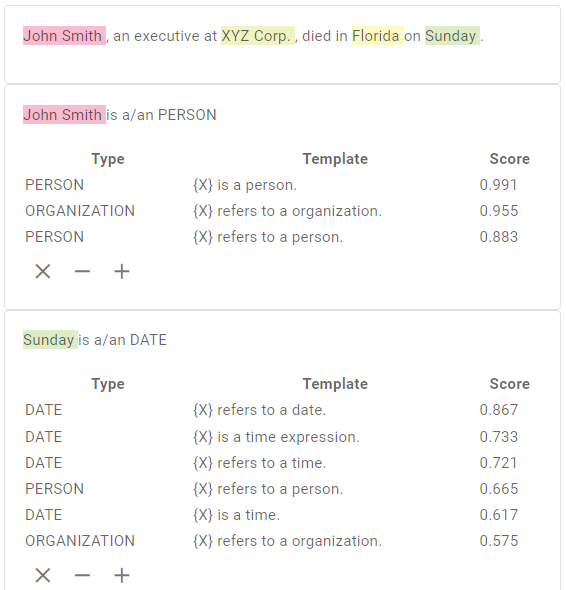
\includegraphics{images/zs4ie_ui.png}
%                 }
%             \end{figure}
%         \end{column}
%     \end{columns}

% \end{frame}

\subsubsection{Conclusions and Limitations}
% \makesubsectiontitlepage

\begin{frame}
    \begin{block}{Conclusions}
        \begin{itemize}[<+->]
            \item \emphasize{Works out of the box}: the approach works without giving any example for training.
            \item \emphasize{Few-shot is easy}: examples from the tasks can be automatically converted to Textual Entailment.
            \item \emphasize{Multi-source learning}: the knowledge from one schema can be transferred to another schema without any mapping.
            \item \emphasize{Time efficiency}: creating verbalizations is more time efficient than annotating examples.
        \end{itemize}
    \end{block}
\end{frame}

\begin{frame}
    \begin{block}{Limitations}
        %The Textual Entailment approach yields promising results, but has its limitations:
        \begin{itemize}[<+->]
            \item \emphasize{Need of span candidates}: the approach classifies spans or span pairs, therefore it requires a span candidate generation step. %It is not well suited for sequence labelling tasks.
            \item \emphasize{Computation efficiency}: the approach requires to perform one inference per verbalization, which can be computationally expensive when the amount of verbalizations is large.
            \item \emphasize{Lack of detail}: verbalizations are prototypical expressions of the type defined, but lack the details and exceptions that are present in the guidelines.
            \item \emphasize{Definition disagreement}: type definition from one dataset to another can vary, and sometimes it cannot be expressed through simple verbalizations.
        \end{itemize}
    \end{block}
\end{frame}

\subsection{Information Extraction with Large Language Models}
\makesubsectiontitlepage

\begin{frame}
    \begin{block}{Motivation}
        \begin{itemize}[<+->]
            \item Large Language Models (LLMs) have shown to be effective in several Natural Language Processing tasks, particularly in low-resource scenarios.
            \item Instruction tunning has shown that LLMs can learn to follow instructions to perform multiple tasks with a single model.
            \item But, current approaches for low-resource Information Extraction ---based on generative LLMs or not--- do not leverage detailed instructions about the task:
                  \begin{itemize}
                      \item They fail when different datasets define a type differently.
                  \end{itemize}
        \end{itemize}
        \blockskip

        \onslide<5-> Can we make use of detailed guidelines to improve the performance of LLMs in Information Extraction tasks?
    \end{block}
\end{frame}

\begin{frame}
    \begin{block}{Challenges}
        In order to teach LLMs to follow guidelines for Information Extraction tasks, we need to address two main challenges:
        \begin{itemize}
            \item How to properly represent the guideline definitions to be used by the LLM?
            \item How to avoid the LLM memorizing the tasks and not attending to the guidelines?
        \end{itemize}
    \end{block}
\end{frame}

\begin{frame}
    \begin{columns}
        \begin{column}{0.35\textwidth}
            \begin{block}{Input-output representation}
                \begin{itemize}
                    \item Labels are defined as Python classes.
                    \item Guidelines are introduced as docstrings in the code.
                    \item Representative candidates are introduced as comments.
                    \item The text is introduced as a variable.
                    \item The result is a list of instances.
                \end{itemize}
            \end{block}
        \end{column}
        \begin{column}{0.6\textwidth}
            \begin{table}
                \centering
                \begin{tabular}{p{\textwidth}}
                    % \texttt{\# The following lines describe the task definition} \\
                    \texttt{\textcolor{github-purple}{@dataclass}}                                                                                                    \\
                    \texttt{\textcolor{github-red}{class} \textcolor{github-dark-red}{Metric}(\textcolor{github-dark-red}{Entity}):}                                  \\
                    \texttt{\textcolor{github-blue}{\quad """Refers to evaluation metrics used to assess}}                                                            \\
                    \texttt{\textcolor{github-blue}{\quad the performance of AI models and algorithms.}}                                                              \\
                    \texttt{\textcolor{github-blue}{\quad Annotate specific metrics like Accuracy."""}}                                                               \\
                    \\
                    \texttt{\quad span: str  \textcolor{github-gray}{\# Such as: "mean squared error",  …}}                                                           \\ \\
                    % \midrule
                    \texttt{text = \textcolor{github-blue}{"The Information Extraction system was evaluated using F1-Score."}}                                \\ \\
                    % \midrule
                    \texttt{result \textcolor{github-red}{=} [\textcolor{github-dark-red}{Metric}(span\textcolor{github-red}{=}\textcolor{github-blue}{"F1-score"})]} \\
                \end{tabular}
            \end{table}
        \end{column}
    \end{columns}
\end{frame}

\begin{frame}
    \begin{block}{Training regularization}
        LLMs can easily memorize the tasks by finding patterns in the input, and consecuently not attending to the guidelines. To avoid this, we propose the following regularizations:
        \begin{itemize}[<+->]
            \item \emphasize{Class order shuffling}: the order of the classes is shuffled for each instance.
            \item \emphasize{Class dropout}: a random percentage of the classes is dropped for each instance and the output is changed accordingly.
            \item \emphasize{Guideline paraphrasing}: the guidelines are paraphrased to avoid the model memorizing the definitions.
            \item \emphasize{Representative candidate sampling}: the representative candidates are sampled from a pool of candidates.
            \item \emphasize{Class name masking}: some class names are masked ---replaced by \inlinepattern{\texttt{LABEL\_1}}--- in the input.
        \end{itemize}

    \end{block}
\end{frame}

% \begin{frame}
%     \begin{block}{Research Questions}
%         \begin{itemize}
%             \item Can LLMs learn to follow guidelines for Information Extraction tasks?
%             \item Are guidelines helpful when data is available? And when it is not?
%         \end{itemize}
%     \end{block}

% \end{frame}

\begin{frame}
    \begin{block}{Research Questions}
        \begin{itemize}
            {\pgfsetfillopacity{1.0}
                \item Are guidelines helpful when data is available? And when it is not?
            }
            {\pgfsetfillopacity{0.2}
                \item How do the guidelines affect seen and unseen labels?
            }
            {\pgfsetfillopacity{0.2}
                \item Where do the errors come from?
                \item Which are the remaining challenges?
            }
        \end{itemize}
    \end{block}
\end{frame}

\begin{frame}
    \begin{block}{Experimental Setup}
        \begin{itemize}
            \item We fine-tuned CodeLlama models \emphasize{with and without using guidelines}.
            \item We divided our pool of datasets into train and eval:
                  \begin{itemize}
                      \item For training we used 9 datasets from \textit{News} and \textit{Biomedical} domains.
                      \item For evaluation we used 10 datasets from \textit{News}, \textit{Biomedical}, \textit{Cybercrime}, \textit{Wikipedia} and more domains.
                  \end{itemize}
        \end{itemize}
    \end{block}

\end{frame}

\begin{frame}
    \begin{block}{Baseline \hspace{14.5em}GoLLIE}
        \begin{columns}[t]
            \begin{column}{0.36\textwidth}
                \begin{table}
                    \vspace{-3.5em}
                    \begin{tabular}{p{\textwidth}}
                        \texttt{\small\textcolor{github-purple}{@dataclass}}                                                                              \\
                        \texttt{\small\textcolor{github-red}{class} \textcolor{github-dark-red}{VulnerabilityPatch}(\textcolor{github-dark-red}{Event}):} \\ \\
                        \texttt{\small\quad mention: str}                                                                                                 \\
                        \texttt{\small\quad cve: \textcolor{github-dark-red}{List}[str]}                                                                  \\
                        \texttt{\small\quad issues: \textcolor{github-dark-red}{List}[str]}                                                               \\
                        \texttt{\small\quad platforms: \textcolor{github-dark-red}{List}[str]}                                                            \\
                        \texttt{\small\quad vulnerability: \textcolor{github-dark-red}{List}[str]}                                                        \\
                        % \texttt{\small\quad vulnerable\_system: \textcolor{github-dark-red}{List}[str]} \\ 
                        \texttt{\small\quad releaser: \textcolor{github-dark-red}{List}[str]}                                                             \\
                    \end{tabular}
                \end{table}
            \end{column}
            \vrule{}
            \begin{column}{0.58\textwidth}
                \begin{table}
                    \vspace{-3.5em}
                    \begin{tabular}{p{\textwidth}}
                        \texttt{\small\textcolor{github-purple}{@dataclass}}                                                                              \\
                        \texttt{\small\textcolor{github-red}{class} \textcolor{github-dark-red}{VulnerabilityPatch}(\textcolor{github-dark-red}{Event}):} \\
                        \texttt{\small\textcolor{github-blue}{\quad """A VulnerabilityPatch Event happens when a}}                                        \\
                        \texttt{\small\textcolor{github-blue}{\quad software company addresses a known vulnerability}}                                    \\
                        \texttt{\small\textcolor{github-blue}{\quad by releasing or describing an update."""}}                                            \\
                        \texttt{\small\quad mention: str}                                                                                                 \\
                        \texttt{\small\textcolor{github-blue}{\quad """The text span that triggers the event.}}                                           \\
                        \texttt{\small\textcolor{github-blue}{\quad Such as: patch, fixed, addresses, implemented"""}}                                    \\
                        \texttt{\small\quad cve: \textcolor{github-dark-red}{List}[str] \textcolor{github-gray}{\# The vulnerability identifier}}         \\
                        \texttt{\small\quad issues: \textcolor{github-dark-red}{List}[str] \textcolor{github-gray}{\# What did the patch fix}}            \\
                        \texttt{\small\quad platforms: \textcolor{github-dark-red}{List}[str] \textcolor{github-gray}{\# The platforms that ...}}         \\
                        \texttt{\small\quad vulnerability: \textcolor{github-dark-red}{List}[str] \textcolor{github-gray}{\# The vulnerability}}          \\
                        % \texttt{\small\quad vulnerable\_system: \textcolor{github-dark-red}{List}[str]} \\ 
                        \texttt{\small\quad releaser: \textcolor{github-dark-red}{List}[str] \textcolor{github-gray}{\# Entity releasing the patch}}      \\
                    \end{tabular}
                \end{table}
            \end{column}
        \end{columns}
    \end{block}

\end{frame}

\begin{frame}
    \begin{columns}[t]
        \begin{column}{0.35\textwidth}
            \begin{block}{Train and evaluation data}
                \begin{itemize}
                    \item Some domains are kept for evaluation only.
                    \item Datasets from different tasks are used:
                    \begin{itemize}
                        \item Named Entity Recognition.
                        \item Relation Extraction.
                        \item Event Extraction.
                        \item Event Argument Extraction.
                        \item Slot Filling.
                    \end{itemize}
                \end{itemize}
            \end{block}
        \end{column}

        \begin{column}{0.55\textwidth}
            \begin{table}
                \vspace{-1.5em}
                \centering
                \resizebox{\textwidth}{!}{
                    \begin{tabular}{l|l|ccccc|cc}
                        \multicolumn{8}{c}{}                                                                                                                                 \\
                        \toprule
                        \textbf{Dataset} & \textbf{Domain} & \textbf{NER} & \textbf{RE} & \textbf{EE} & \textbf{EAE} & \textbf{SF} & \textbf{Training} & \textbf{Evaluation} \\
                        \midrule
                        ACE05            & News            & \checkmark   & \checkmark  & \checkmark  & \checkmark   &             & \checkmark        & \checkmark          \\
                        BC5CDR           & Biomedical      & \checkmark   &             &             &              &             & \checkmark        & \checkmark          \\
                        CoNLL 2003       & News            & \checkmark   &             &             &              &             & \checkmark        & \checkmark          \\
                        DIANN            & Biomedical      & \checkmark   &             &             &              &             & \checkmark        & \checkmark          \\
                        NCBIDisease      & Biomedical      & \checkmark   &             &             &              &             & \checkmark        & \checkmark          \\
                        Ontonotes 5      & News            & \checkmark   &             &             &              &             & \checkmark        & \checkmark          \\
                        RAMS             & News            &              &             &             & \checkmark   &             & \checkmark        & \checkmark          \\
                        TACRED           & News            &              &             &             &              & \checkmark  & \checkmark        & \checkmark          \\
                        WNUT 2017        & News            & \checkmark   &             &             &              &             & \checkmark        & \checkmark          \\
                        \midrule
                        BroadTwitter     & Twitter         & \checkmark   &             &             &              &             &                   & \checkmark          \\
                        CASIE            & Cybercrime      &              &             & \checkmark  & \checkmark   &             &                   & \checkmark          \\
                        CrossNER         & \textit{Many}   & \checkmark   &             &             &              &             &                   & \checkmark          \\
                        E3C              & Biomedical      & \checkmark   &             &             &              &             &                   & \checkmark          \\
                        FabNER           & Science         & \checkmark   &             &             &              &             &                   & \checkmark          \\
                        HarveyNER        & Twitter         & \checkmark   &             &             &              &             &                   & \checkmark          \\
                        MIT Movie        & Queries         & \checkmark   &             &             &              &             &                   & \checkmark          \\
                        MIT Restaurants  & Queries         & \checkmark   &             &             &              &             &                   & \checkmark          \\
                        MultiNERD        & Wikipedia       & \checkmark   &             &             &              &             &                   & \checkmark          \\
                        WikiEvents       & Wikipedia       & \checkmark   &             & \checkmark  & \checkmark   &             &                   & \checkmark          \\
                        \bottomrule
                    \end{tabular}
                }
                \caption{Datasets used on the experiments.}
            \end{table}
        \end{column}
    \end{columns}
    

\end{frame}

\begin{frame}
    \begin{block}{Evaluation results}
        \begin{figure}
            \centering
            \resizebox{.6\textwidth}{!}{
                %% Creator: Matplotlib, PGF backend
%%
%% To include the figure in your LaTeX document, write
%%   \input{<filename>.pgf}
%%
%% Make sure the required packages are loaded in your preamble
%%   \usepackage{pgf}
%%
%% Also ensure that all the required font packages are loaded; for instance,
%% the lmodern package is sometimes necessary when using math font.
%%   \usepackage{lmodern}
%%
%% Figures using additional raster images can only be included by \input if
%% they are in the same directory as the main LaTeX file. For loading figures
%% from other directories you can use the `import` package
%%   \usepackage{import}
%%
%% and then include the figures with
%%   \import{<path to file>}{<filename>.pgf}
%%
%% Matplotlib used the following preamble
%%   \def\mathdefault#1{#1}
%%   \everymath=\expandafter{\the\everymath\displaystyle}
%%   
%%   \ifdefined\pdftexversion\else  % non-pdftex case.
%%     \usepackage{fontspec}
%%   \fi
%%   \makeatletter\@ifpackageloaded{underscore}{}{\usepackage[strings]{underscore}}\makeatother
%%
\begingroup%
\makeatletter%
\begin{pgfpicture}%
\pgfpathrectangle{\pgfpointorigin}{\pgfqpoint{7.563790in}{3.861108in}}%
\pgfusepath{use as bounding box, clip}%
\begin{pgfscope}%
\pgfsetbuttcap%
\pgfsetmiterjoin%
\definecolor{currentfill}{rgb}{1.000000,1.000000,1.000000}%
\pgfsetfillcolor{currentfill}%
\pgfsetlinewidth{0.000000pt}%
\definecolor{currentstroke}{rgb}{1.000000,1.000000,1.000000}%
\pgfsetstrokecolor{currentstroke}%
\pgfsetdash{}{0pt}%
\pgfpathmoveto{\pgfqpoint{-0.000000in}{0.000000in}}%
\pgfpathlineto{\pgfqpoint{7.563790in}{0.000000in}}%
\pgfpathlineto{\pgfqpoint{7.563790in}{3.861108in}}%
\pgfpathlineto{\pgfqpoint{-0.000000in}{3.861108in}}%
\pgfpathlineto{\pgfqpoint{-0.000000in}{0.000000in}}%
\pgfpathclose%
\pgfusepath{fill}%
\end{pgfscope}%
\begin{pgfscope}%
\pgfsetbuttcap%
\pgfsetmiterjoin%
\definecolor{currentfill}{rgb}{1.000000,1.000000,1.000000}%
\pgfsetfillcolor{currentfill}%
\pgfsetlinewidth{0.000000pt}%
\definecolor{currentstroke}{rgb}{0.000000,0.000000,0.000000}%
\pgfsetstrokecolor{currentstroke}%
\pgfsetstrokeopacity{0.000000}%
\pgfsetdash{}{0pt}%
\pgfpathmoveto{\pgfqpoint{0.744398in}{0.531944in}}%
\pgfpathlineto{\pgfqpoint{7.240225in}{0.531944in}}%
\pgfpathlineto{\pgfqpoint{7.240225in}{3.399987in}}%
\pgfpathlineto{\pgfqpoint{0.744398in}{3.399987in}}%
\pgfpathlineto{\pgfqpoint{0.744398in}{0.531944in}}%
\pgfpathclose%
\pgfusepath{fill}%
\end{pgfscope}%
\begin{pgfscope}%
\pgfpathrectangle{\pgfqpoint{0.744398in}{0.531944in}}{\pgfqpoint{6.495827in}{2.868044in}}%
\pgfusepath{clip}%
\pgfsetroundcap%
\pgfsetroundjoin%
\pgfsetlinewidth{0.803000pt}%
\definecolor{currentstroke}{rgb}{0.800000,0.800000,0.800000}%
\pgfsetstrokecolor{currentstroke}%
\pgfsetstrokeopacity{0.000000}%
\pgfsetdash{}{0pt}%
\pgfpathmoveto{\pgfqpoint{2.135300in}{0.531944in}}%
\pgfpathlineto{\pgfqpoint{2.135300in}{3.399987in}}%
\pgfusepath{stroke}%
\end{pgfscope}%
\begin{pgfscope}%
\definecolor{textcolor}{rgb}{0.150000,0.150000,0.150000}%
\pgfsetstrokecolor{textcolor}%
\pgfsetfillcolor{textcolor}%
\pgftext[x=2.135300in, y=0.344444in, left, base]{\color{textcolor}{\sffamily\fontsize{14.000000}{16.800000}\selectfont\catcode`\^=\active\def^{\ifmmode\sp\else\^{}\fi}\catcode`\%=\active\def%{\%}}}%
\end{pgfscope}%
\begin{pgfscope}%
\definecolor{textcolor}{rgb}{0.150000,0.150000,0.150000}%
\pgfsetstrokecolor{textcolor}%
\pgfsetfillcolor{textcolor}%
\pgftext[x=1.701822in, y=0.138889in, left, base]{\color{textcolor}{\sffamily\fontsize{14.000000}{16.800000}\selectfont\catcode`\^=\active\def^{\ifmmode\sp\else\^{}\fi}\catcode`\%=\active\def%{\%}Supervised}}%
\end{pgfscope}%
\begin{pgfscope}%
\pgfpathrectangle{\pgfqpoint{0.744398in}{0.531944in}}{\pgfqpoint{6.495827in}{2.868044in}}%
\pgfusepath{clip}%
\pgfsetroundcap%
\pgfsetroundjoin%
\pgfsetlinewidth{0.803000pt}%
\definecolor{currentstroke}{rgb}{0.800000,0.800000,0.800000}%
\pgfsetstrokecolor{currentstroke}%
\pgfsetstrokeopacity{0.000000}%
\pgfsetdash{}{0pt}%
\pgfpathmoveto{\pgfqpoint{5.849323in}{0.531944in}}%
\pgfpathlineto{\pgfqpoint{5.849323in}{3.399987in}}%
\pgfusepath{stroke}%
\end{pgfscope}%
\begin{pgfscope}%
\definecolor{textcolor}{rgb}{0.150000,0.150000,0.150000}%
\pgfsetstrokecolor{textcolor}%
\pgfsetfillcolor{textcolor}%
\pgftext[x=5.849323in, y=0.344444in, left, base]{\color{textcolor}{\sffamily\fontsize{14.000000}{16.800000}\selectfont\catcode`\^=\active\def^{\ifmmode\sp\else\^{}\fi}\catcode`\%=\active\def%{\%}}}%
\end{pgfscope}%
\begin{pgfscope}%
\definecolor{textcolor}{rgb}{0.150000,0.150000,0.150000}%
\pgfsetstrokecolor{textcolor}%
\pgfsetfillcolor{textcolor}%
\pgftext[x=5.442153in, y=0.138889in, left, base]{\color{textcolor}{\sffamily\fontsize{14.000000}{16.800000}\selectfont\catcode`\^=\active\def^{\ifmmode\sp\else\^{}\fi}\catcode`\%=\active\def%{\%}Zero-Shot}}%
\end{pgfscope}%
\begin{pgfscope}%
\pgfpathrectangle{\pgfqpoint{0.744398in}{0.531944in}}{\pgfqpoint{6.495827in}{2.868044in}}%
\pgfusepath{clip}%
\pgfsetbuttcap%
\pgfsetroundjoin%
\pgfsetlinewidth{0.803000pt}%
\definecolor{currentstroke}{rgb}{0.800000,0.800000,0.800000}%
\pgfsetstrokecolor{currentstroke}%
\pgfsetstrokeopacity{0.750000}%
\pgfsetdash{{2.960000pt}{1.280000pt}}{0.000000pt}%
\pgfpathmoveto{\pgfqpoint{0.744398in}{0.531944in}}%
\pgfpathlineto{\pgfqpoint{7.240225in}{0.531944in}}%
\pgfusepath{stroke}%
\end{pgfscope}%
\begin{pgfscope}%
\definecolor{textcolor}{rgb}{0.150000,0.150000,0.150000}%
\pgfsetstrokecolor{textcolor}%
\pgfsetfillcolor{textcolor}%
\pgftext[x=0.626342in, y=0.483718in, left, base]{\color{textcolor}{\sffamily\fontsize{10.000000}{12.000000}\selectfont\catcode`\^=\active\def^{\ifmmode\sp\else\^{}\fi}\catcode`\%=\active\def%{\%}$\mathdefault{0}$}}%
\end{pgfscope}%
\begin{pgfscope}%
\pgfpathrectangle{\pgfqpoint{0.744398in}{0.531944in}}{\pgfqpoint{6.495827in}{2.868044in}}%
\pgfusepath{clip}%
\pgfsetbuttcap%
\pgfsetroundjoin%
\pgfsetlinewidth{0.803000pt}%
\definecolor{currentstroke}{rgb}{0.800000,0.800000,0.800000}%
\pgfsetstrokecolor{currentstroke}%
\pgfsetstrokeopacity{0.750000}%
\pgfsetdash{{2.960000pt}{1.280000pt}}{0.000000pt}%
\pgfpathmoveto{\pgfqpoint{0.744398in}{0.896140in}}%
\pgfpathlineto{\pgfqpoint{7.240225in}{0.896140in}}%
\pgfusepath{stroke}%
\end{pgfscope}%
\begin{pgfscope}%
\definecolor{textcolor}{rgb}{0.150000,0.150000,0.150000}%
\pgfsetstrokecolor{textcolor}%
\pgfsetfillcolor{textcolor}%
\pgftext[x=0.556898in, y=0.847914in, left, base]{\color{textcolor}{\sffamily\fontsize{10.000000}{12.000000}\selectfont\catcode`\^=\active\def^{\ifmmode\sp\else\^{}\fi}\catcode`\%=\active\def%{\%}$\mathdefault{10}$}}%
\end{pgfscope}%
\begin{pgfscope}%
\pgfpathrectangle{\pgfqpoint{0.744398in}{0.531944in}}{\pgfqpoint{6.495827in}{2.868044in}}%
\pgfusepath{clip}%
\pgfsetbuttcap%
\pgfsetroundjoin%
\pgfsetlinewidth{0.803000pt}%
\definecolor{currentstroke}{rgb}{0.800000,0.800000,0.800000}%
\pgfsetstrokecolor{currentstroke}%
\pgfsetstrokeopacity{0.750000}%
\pgfsetdash{{2.960000pt}{1.280000pt}}{0.000000pt}%
\pgfpathmoveto{\pgfqpoint{0.744398in}{1.260336in}}%
\pgfpathlineto{\pgfqpoint{7.240225in}{1.260336in}}%
\pgfusepath{stroke}%
\end{pgfscope}%
\begin{pgfscope}%
\definecolor{textcolor}{rgb}{0.150000,0.150000,0.150000}%
\pgfsetstrokecolor{textcolor}%
\pgfsetfillcolor{textcolor}%
\pgftext[x=0.556898in, y=1.212110in, left, base]{\color{textcolor}{\sffamily\fontsize{10.000000}{12.000000}\selectfont\catcode`\^=\active\def^{\ifmmode\sp\else\^{}\fi}\catcode`\%=\active\def%{\%}$\mathdefault{20}$}}%
\end{pgfscope}%
\begin{pgfscope}%
\pgfpathrectangle{\pgfqpoint{0.744398in}{0.531944in}}{\pgfqpoint{6.495827in}{2.868044in}}%
\pgfusepath{clip}%
\pgfsetbuttcap%
\pgfsetroundjoin%
\pgfsetlinewidth{0.803000pt}%
\definecolor{currentstroke}{rgb}{0.800000,0.800000,0.800000}%
\pgfsetstrokecolor{currentstroke}%
\pgfsetstrokeopacity{0.750000}%
\pgfsetdash{{2.960000pt}{1.280000pt}}{0.000000pt}%
\pgfpathmoveto{\pgfqpoint{0.744398in}{1.624532in}}%
\pgfpathlineto{\pgfqpoint{7.240225in}{1.624532in}}%
\pgfusepath{stroke}%
\end{pgfscope}%
\begin{pgfscope}%
\definecolor{textcolor}{rgb}{0.150000,0.150000,0.150000}%
\pgfsetstrokecolor{textcolor}%
\pgfsetfillcolor{textcolor}%
\pgftext[x=0.556898in, y=1.576306in, left, base]{\color{textcolor}{\sffamily\fontsize{10.000000}{12.000000}\selectfont\catcode`\^=\active\def^{\ifmmode\sp\else\^{}\fi}\catcode`\%=\active\def%{\%}$\mathdefault{30}$}}%
\end{pgfscope}%
\begin{pgfscope}%
\pgfpathrectangle{\pgfqpoint{0.744398in}{0.531944in}}{\pgfqpoint{6.495827in}{2.868044in}}%
\pgfusepath{clip}%
\pgfsetbuttcap%
\pgfsetroundjoin%
\pgfsetlinewidth{0.803000pt}%
\definecolor{currentstroke}{rgb}{0.800000,0.800000,0.800000}%
\pgfsetstrokecolor{currentstroke}%
\pgfsetstrokeopacity{0.750000}%
\pgfsetdash{{2.960000pt}{1.280000pt}}{0.000000pt}%
\pgfpathmoveto{\pgfqpoint{0.744398in}{1.988728in}}%
\pgfpathlineto{\pgfqpoint{7.240225in}{1.988728in}}%
\pgfusepath{stroke}%
\end{pgfscope}%
\begin{pgfscope}%
\definecolor{textcolor}{rgb}{0.150000,0.150000,0.150000}%
\pgfsetstrokecolor{textcolor}%
\pgfsetfillcolor{textcolor}%
\pgftext[x=0.556898in, y=1.940502in, left, base]{\color{textcolor}{\sffamily\fontsize{10.000000}{12.000000}\selectfont\catcode`\^=\active\def^{\ifmmode\sp\else\^{}\fi}\catcode`\%=\active\def%{\%}$\mathdefault{40}$}}%
\end{pgfscope}%
\begin{pgfscope}%
\pgfpathrectangle{\pgfqpoint{0.744398in}{0.531944in}}{\pgfqpoint{6.495827in}{2.868044in}}%
\pgfusepath{clip}%
\pgfsetbuttcap%
\pgfsetroundjoin%
\pgfsetlinewidth{0.803000pt}%
\definecolor{currentstroke}{rgb}{0.800000,0.800000,0.800000}%
\pgfsetstrokecolor{currentstroke}%
\pgfsetstrokeopacity{0.750000}%
\pgfsetdash{{2.960000pt}{1.280000pt}}{0.000000pt}%
\pgfpathmoveto{\pgfqpoint{0.744398in}{2.352924in}}%
\pgfpathlineto{\pgfqpoint{7.240225in}{2.352924in}}%
\pgfusepath{stroke}%
\end{pgfscope}%
\begin{pgfscope}%
\definecolor{textcolor}{rgb}{0.150000,0.150000,0.150000}%
\pgfsetstrokecolor{textcolor}%
\pgfsetfillcolor{textcolor}%
\pgftext[x=0.556898in, y=2.304698in, left, base]{\color{textcolor}{\sffamily\fontsize{10.000000}{12.000000}\selectfont\catcode`\^=\active\def^{\ifmmode\sp\else\^{}\fi}\catcode`\%=\active\def%{\%}$\mathdefault{50}$}}%
\end{pgfscope}%
\begin{pgfscope}%
\pgfpathrectangle{\pgfqpoint{0.744398in}{0.531944in}}{\pgfqpoint{6.495827in}{2.868044in}}%
\pgfusepath{clip}%
\pgfsetbuttcap%
\pgfsetroundjoin%
\pgfsetlinewidth{0.803000pt}%
\definecolor{currentstroke}{rgb}{0.800000,0.800000,0.800000}%
\pgfsetstrokecolor{currentstroke}%
\pgfsetstrokeopacity{0.750000}%
\pgfsetdash{{2.960000pt}{1.280000pt}}{0.000000pt}%
\pgfpathmoveto{\pgfqpoint{0.744398in}{2.717120in}}%
\pgfpathlineto{\pgfqpoint{7.240225in}{2.717120in}}%
\pgfusepath{stroke}%
\end{pgfscope}%
\begin{pgfscope}%
\definecolor{textcolor}{rgb}{0.150000,0.150000,0.150000}%
\pgfsetstrokecolor{textcolor}%
\pgfsetfillcolor{textcolor}%
\pgftext[x=0.556898in, y=2.668894in, left, base]{\color{textcolor}{\sffamily\fontsize{10.000000}{12.000000}\selectfont\catcode`\^=\active\def^{\ifmmode\sp\else\^{}\fi}\catcode`\%=\active\def%{\%}$\mathdefault{60}$}}%
\end{pgfscope}%
\begin{pgfscope}%
\pgfpathrectangle{\pgfqpoint{0.744398in}{0.531944in}}{\pgfqpoint{6.495827in}{2.868044in}}%
\pgfusepath{clip}%
\pgfsetbuttcap%
\pgfsetroundjoin%
\pgfsetlinewidth{0.803000pt}%
\definecolor{currentstroke}{rgb}{0.800000,0.800000,0.800000}%
\pgfsetstrokecolor{currentstroke}%
\pgfsetstrokeopacity{0.750000}%
\pgfsetdash{{2.960000pt}{1.280000pt}}{0.000000pt}%
\pgfpathmoveto{\pgfqpoint{0.744398in}{3.081316in}}%
\pgfpathlineto{\pgfqpoint{7.240225in}{3.081316in}}%
\pgfusepath{stroke}%
\end{pgfscope}%
\begin{pgfscope}%
\definecolor{textcolor}{rgb}{0.150000,0.150000,0.150000}%
\pgfsetstrokecolor{textcolor}%
\pgfsetfillcolor{textcolor}%
\pgftext[x=0.556898in, y=3.033090in, left, base]{\color{textcolor}{\sffamily\fontsize{10.000000}{12.000000}\selectfont\catcode`\^=\active\def^{\ifmmode\sp\else\^{}\fi}\catcode`\%=\active\def%{\%}$\mathdefault{70}$}}%
\end{pgfscope}%
\begin{pgfscope}%
\definecolor{textcolor}{rgb}{0.150000,0.150000,0.150000}%
\pgfsetstrokecolor{textcolor}%
\pgfsetfillcolor{textcolor}%
\pgftext[x=0.501342in,y=1.965965in,,bottom,rotate=90.000000]{\color{textcolor}{\sffamily\fontsize{14.000000}{16.800000}\selectfont\catcode`\^=\active\def^{\ifmmode\sp\else\^{}\fi}\catcode`\%=\active\def%{\%}F1 Score}}%
\end{pgfscope}%
\begin{pgfscope}%
\pgfpathrectangle{\pgfqpoint{0.744398in}{0.531944in}}{\pgfqpoint{6.495827in}{2.868044in}}%
\pgfusepath{clip}%
\pgfsetbuttcap%
\pgfsetmiterjoin%
\definecolor{currentfill}{rgb}{0.031373,0.270588,0.494118}%
\pgfsetfillcolor{currentfill}%
\pgfsetfillopacity{0.500000}%
\pgfsetlinewidth{1.003750pt}%
\definecolor{currentstroke}{rgb}{0.031373,0.270588,0.494118}%
\pgfsetstrokecolor{currentstroke}%
\pgfsetstrokeopacity{0.500000}%
\pgfsetdash{}{0pt}%
\pgfpathmoveto{\pgfqpoint{1.039663in}{0.531944in}}%
\pgfpathlineto{\pgfqpoint{1.559626in}{0.531944in}}%
\pgfpathlineto{\pgfqpoint{1.559626in}{3.201500in}}%
\pgfpathlineto{\pgfqpoint{1.039663in}{3.201500in}}%
\pgfpathlineto{\pgfqpoint{1.039663in}{0.531944in}}%
\pgfpathclose%
\pgfusepath{stroke,fill}%
\end{pgfscope}%
\begin{pgfscope}%
\pgfpathrectangle{\pgfqpoint{0.744398in}{0.531944in}}{\pgfqpoint{6.495827in}{2.868044in}}%
\pgfusepath{clip}%
\pgfsetbuttcap%
\pgfsetmiterjoin%
\definecolor{currentfill}{rgb}{0.294118,0.086275,0.996078}%
\pgfsetfillcolor{currentfill}%
\pgfsetfillopacity{0.500000}%
\pgfsetlinewidth{1.003750pt}%
\definecolor{currentstroke}{rgb}{0.294118,0.086275,0.996078}%
\pgfsetstrokecolor{currentstroke}%
\pgfsetstrokeopacity{0.500000}%
\pgfsetdash{}{0pt}%
\pgfpathmoveto{\pgfqpoint{1.596767in}{0.531944in}}%
\pgfpathlineto{\pgfqpoint{2.116730in}{0.531944in}}%
\pgfpathlineto{\pgfqpoint{2.116730in}{3.190574in}}%
\pgfpathlineto{\pgfqpoint{1.596767in}{3.190574in}}%
\pgfpathlineto{\pgfqpoint{1.596767in}{0.531944in}}%
\pgfpathclose%
\pgfusepath{stroke,fill}%
\end{pgfscope}%
\begin{pgfscope}%
\pgfpathrectangle{\pgfqpoint{0.744398in}{0.531944in}}{\pgfqpoint{6.495827in}{2.868044in}}%
\pgfusepath{clip}%
\pgfsetbuttcap%
\pgfsetmiterjoin%
\definecolor{currentfill}{rgb}{0.294118,0.086275,0.996078}%
\pgfsetfillcolor{currentfill}%
\pgfsetfillopacity{0.250000}%
\pgfsetlinewidth{1.003750pt}%
\definecolor{currentstroke}{rgb}{0.294118,0.086275,0.996078}%
\pgfsetstrokecolor{currentstroke}%
\pgfsetstrokeopacity{0.250000}%
\pgfsetdash{}{0pt}%
\pgfpathmoveto{\pgfqpoint{2.153870in}{0.531944in}}%
\pgfpathlineto{\pgfqpoint{2.673833in}{0.531944in}}%
\pgfpathlineto{\pgfqpoint{2.673833in}{3.223352in}}%
\pgfpathlineto{\pgfqpoint{2.153870in}{3.223352in}}%
\pgfpathlineto{\pgfqpoint{2.153870in}{0.531944in}}%
\pgfpathclose%
\pgfusepath{stroke,fill}%
\end{pgfscope}%
\begin{pgfscope}%
\pgfsetbuttcap%
\pgfsetmiterjoin%
\definecolor{currentfill}{rgb}{0.294118,0.086275,0.996078}%
\pgfsetfillcolor{currentfill}%
\pgfsetfillopacity{0.250000}%
\pgfsetlinewidth{1.003750pt}%
\definecolor{currentstroke}{rgb}{0.294118,0.086275,0.996078}%
\pgfsetstrokecolor{currentstroke}%
\pgfsetstrokeopacity{0.250000}%
\pgfsetdash{}{0pt}%
\pgfpathrectangle{\pgfqpoint{0.744398in}{0.531944in}}{\pgfqpoint{6.495827in}{2.868044in}}%
\pgfusepath{clip}%
\pgfpathmoveto{\pgfqpoint{2.153870in}{0.531944in}}%
\pgfpathlineto{\pgfqpoint{2.673833in}{0.531944in}}%
\pgfpathlineto{\pgfqpoint{2.673833in}{3.223352in}}%
\pgfpathlineto{\pgfqpoint{2.153870in}{3.223352in}}%
\pgfpathlineto{\pgfqpoint{2.153870in}{0.531944in}}%
\pgfpathclose%
\pgfusepath{clip}%
\pgfsys@defobject{currentpattern}{\pgfqpoint{0in}{0in}}{\pgfqpoint{1in}{1in}}{%
\begin{pgfscope}%
\pgfpathrectangle{\pgfqpoint{0in}{0in}}{\pgfqpoint{1in}{1in}}%
\pgfusepath{clip}%
\pgfpathmoveto{\pgfqpoint{-0.500000in}{0.500000in}}%
\pgfpathlineto{\pgfqpoint{0.500000in}{1.500000in}}%
\pgfpathmoveto{\pgfqpoint{-0.333333in}{0.333333in}}%
\pgfpathlineto{\pgfqpoint{0.666667in}{1.333333in}}%
\pgfpathmoveto{\pgfqpoint{-0.166667in}{0.166667in}}%
\pgfpathlineto{\pgfqpoint{0.833333in}{1.166667in}}%
\pgfpathmoveto{\pgfqpoint{0.000000in}{0.000000in}}%
\pgfpathlineto{\pgfqpoint{1.000000in}{1.000000in}}%
\pgfpathmoveto{\pgfqpoint{0.166667in}{-0.166667in}}%
\pgfpathlineto{\pgfqpoint{1.166667in}{0.833333in}}%
\pgfpathmoveto{\pgfqpoint{0.333333in}{-0.333333in}}%
\pgfpathlineto{\pgfqpoint{1.333333in}{0.666667in}}%
\pgfpathmoveto{\pgfqpoint{0.500000in}{-0.500000in}}%
\pgfpathlineto{\pgfqpoint{1.500000in}{0.500000in}}%
\pgfusepath{stroke}%
\end{pgfscope}%
}%
\pgfsys@transformshift{2.153870in}{0.531944in}%
\pgfsys@useobject{currentpattern}{}%
\pgfsys@transformshift{1in}{0in}%
\pgfsys@transformshift{-1in}{0in}%
\pgfsys@transformshift{0in}{1in}%
\pgfsys@useobject{currentpattern}{}%
\pgfsys@transformshift{1in}{0in}%
\pgfsys@transformshift{-1in}{0in}%
\pgfsys@transformshift{0in}{1in}%
\pgfsys@useobject{currentpattern}{}%
\pgfsys@transformshift{1in}{0in}%
\pgfsys@transformshift{-1in}{0in}%
\pgfsys@transformshift{0in}{1in}%
\end{pgfscope}%
\begin{pgfscope}%
\pgfpathrectangle{\pgfqpoint{0.744398in}{0.531944in}}{\pgfqpoint{6.495827in}{2.868044in}}%
\pgfusepath{clip}%
\pgfsetbuttcap%
\pgfsetmiterjoin%
\definecolor{currentfill}{rgb}{0.294118,0.086275,0.996078}%
\pgfsetfillcolor{currentfill}%
\pgfsetfillopacity{0.250000}%
\pgfsetlinewidth{1.003750pt}%
\definecolor{currentstroke}{rgb}{0.294118,0.086275,0.996078}%
\pgfsetstrokecolor{currentstroke}%
\pgfsetstrokeopacity{0.250000}%
\pgfsetdash{}{0pt}%
\pgfpathmoveto{\pgfqpoint{2.710974in}{0.531944in}}%
\pgfpathlineto{\pgfqpoint{3.230937in}{0.531944in}}%
\pgfpathlineto{\pgfqpoint{3.230937in}{3.263414in}}%
\pgfpathlineto{\pgfqpoint{2.710974in}{3.263414in}}%
\pgfpathlineto{\pgfqpoint{2.710974in}{0.531944in}}%
\pgfpathclose%
\pgfusepath{stroke,fill}%
\end{pgfscope}%
\begin{pgfscope}%
\pgfsetbuttcap%
\pgfsetmiterjoin%
\definecolor{currentfill}{rgb}{0.294118,0.086275,0.996078}%
\pgfsetfillcolor{currentfill}%
\pgfsetfillopacity{0.250000}%
\pgfsetlinewidth{1.003750pt}%
\definecolor{currentstroke}{rgb}{0.294118,0.086275,0.996078}%
\pgfsetstrokecolor{currentstroke}%
\pgfsetstrokeopacity{0.250000}%
\pgfsetdash{}{0pt}%
\pgfpathrectangle{\pgfqpoint{0.744398in}{0.531944in}}{\pgfqpoint{6.495827in}{2.868044in}}%
\pgfusepath{clip}%
\pgfpathmoveto{\pgfqpoint{2.710974in}{0.531944in}}%
\pgfpathlineto{\pgfqpoint{3.230937in}{0.531944in}}%
\pgfpathlineto{\pgfqpoint{3.230937in}{3.263414in}}%
\pgfpathlineto{\pgfqpoint{2.710974in}{3.263414in}}%
\pgfpathlineto{\pgfqpoint{2.710974in}{0.531944in}}%
\pgfpathclose%
\pgfusepath{clip}%
\pgfsys@defobject{currentpattern}{\pgfqpoint{0in}{0in}}{\pgfqpoint{1in}{1in}}{%
\begin{pgfscope}%
\pgfpathrectangle{\pgfqpoint{0in}{0in}}{\pgfqpoint{1in}{1in}}%
\pgfusepath{clip}%
\pgfpathmoveto{\pgfqpoint{-0.500000in}{0.500000in}}%
\pgfpathlineto{\pgfqpoint{0.500000in}{-0.500000in}}%
\pgfpathmoveto{\pgfqpoint{-0.333333in}{0.666667in}}%
\pgfpathlineto{\pgfqpoint{0.666667in}{-0.333333in}}%
\pgfpathmoveto{\pgfqpoint{-0.166667in}{0.833333in}}%
\pgfpathlineto{\pgfqpoint{0.833333in}{-0.166667in}}%
\pgfpathmoveto{\pgfqpoint{0.000000in}{1.000000in}}%
\pgfpathlineto{\pgfqpoint{1.000000in}{0.000000in}}%
\pgfpathmoveto{\pgfqpoint{0.166667in}{1.166667in}}%
\pgfpathlineto{\pgfqpoint{1.166667in}{0.166667in}}%
\pgfpathmoveto{\pgfqpoint{0.333333in}{1.333333in}}%
\pgfpathlineto{\pgfqpoint{1.333333in}{0.333333in}}%
\pgfpathmoveto{\pgfqpoint{0.500000in}{1.500000in}}%
\pgfpathlineto{\pgfqpoint{1.500000in}{0.500000in}}%
\pgfusepath{stroke}%
\end{pgfscope}%
}%
\pgfsys@transformshift{2.710974in}{0.531944in}%
\pgfsys@useobject{currentpattern}{}%
\pgfsys@transformshift{1in}{0in}%
\pgfsys@transformshift{-1in}{0in}%
\pgfsys@transformshift{0in}{1in}%
\pgfsys@useobject{currentpattern}{}%
\pgfsys@transformshift{1in}{0in}%
\pgfsys@transformshift{-1in}{0in}%
\pgfsys@transformshift{0in}{1in}%
\pgfsys@useobject{currentpattern}{}%
\pgfsys@transformshift{1in}{0in}%
\pgfsys@transformshift{-1in}{0in}%
\pgfsys@transformshift{0in}{1in}%
\end{pgfscope}%
\begin{pgfscope}%
\pgfpathrectangle{\pgfqpoint{0.744398in}{0.531944in}}{\pgfqpoint{6.495827in}{2.868044in}}%
\pgfusepath{clip}%
\pgfsetbuttcap%
\pgfsetmiterjoin%
\definecolor{currentfill}{rgb}{0.031373,0.270588,0.494118}%
\pgfsetfillcolor{currentfill}%
\pgfsetfillopacity{0.500000}%
\pgfsetlinewidth{1.003750pt}%
\definecolor{currentstroke}{rgb}{0.031373,0.270588,0.494118}%
\pgfsetstrokecolor{currentstroke}%
\pgfsetstrokeopacity{0.500000}%
\pgfsetdash{}{0pt}%
\pgfpathmoveto{\pgfqpoint{4.753686in}{0.531944in}}%
\pgfpathlineto{\pgfqpoint{5.273650in}{0.531944in}}%
\pgfpathlineto{\pgfqpoint{5.273650in}{2.072493in}}%
\pgfpathlineto{\pgfqpoint{4.753686in}{2.072493in}}%
\pgfpathlineto{\pgfqpoint{4.753686in}{0.531944in}}%
\pgfpathclose%
\pgfusepath{stroke,fill}%
\end{pgfscope}%
\begin{pgfscope}%
\pgfpathrectangle{\pgfqpoint{0.744398in}{0.531944in}}{\pgfqpoint{6.495827in}{2.868044in}}%
\pgfusepath{clip}%
\pgfsetbuttcap%
\pgfsetmiterjoin%
\definecolor{currentfill}{rgb}{0.294118,0.086275,0.996078}%
\pgfsetfillcolor{currentfill}%
\pgfsetfillopacity{0.500000}%
\pgfsetlinewidth{1.003750pt}%
\definecolor{currentstroke}{rgb}{0.294118,0.086275,0.996078}%
\pgfsetstrokecolor{currentstroke}%
\pgfsetstrokeopacity{0.500000}%
\pgfsetdash{}{0pt}%
\pgfpathmoveto{\pgfqpoint{5.310790in}{0.531944in}}%
\pgfpathlineto{\pgfqpoint{5.830753in}{0.531944in}}%
\pgfpathlineto{\pgfqpoint{5.830753in}{2.545947in}}%
\pgfpathlineto{\pgfqpoint{5.310790in}{2.545947in}}%
\pgfpathlineto{\pgfqpoint{5.310790in}{0.531944in}}%
\pgfpathclose%
\pgfusepath{stroke,fill}%
\end{pgfscope}%
\begin{pgfscope}%
\pgfpathrectangle{\pgfqpoint{0.744398in}{0.531944in}}{\pgfqpoint{6.495827in}{2.868044in}}%
\pgfusepath{clip}%
\pgfsetbuttcap%
\pgfsetmiterjoin%
\definecolor{currentfill}{rgb}{0.294118,0.086275,0.996078}%
\pgfsetfillcolor{currentfill}%
\pgfsetfillopacity{0.250000}%
\pgfsetlinewidth{1.003750pt}%
\definecolor{currentstroke}{rgb}{0.294118,0.086275,0.996078}%
\pgfsetstrokecolor{currentstroke}%
\pgfsetstrokeopacity{0.250000}%
\pgfsetdash{}{0pt}%
\pgfpathmoveto{\pgfqpoint{5.867893in}{0.531944in}}%
\pgfpathlineto{\pgfqpoint{6.387857in}{0.531944in}}%
\pgfpathlineto{\pgfqpoint{6.387857in}{2.571441in}}%
\pgfpathlineto{\pgfqpoint{5.867893in}{2.571441in}}%
\pgfpathlineto{\pgfqpoint{5.867893in}{0.531944in}}%
\pgfpathclose%
\pgfusepath{stroke,fill}%
\end{pgfscope}%
\begin{pgfscope}%
\pgfsetbuttcap%
\pgfsetmiterjoin%
\definecolor{currentfill}{rgb}{0.294118,0.086275,0.996078}%
\pgfsetfillcolor{currentfill}%
\pgfsetfillopacity{0.250000}%
\pgfsetlinewidth{1.003750pt}%
\definecolor{currentstroke}{rgb}{0.294118,0.086275,0.996078}%
\pgfsetstrokecolor{currentstroke}%
\pgfsetstrokeopacity{0.250000}%
\pgfsetdash{}{0pt}%
\pgfpathrectangle{\pgfqpoint{0.744398in}{0.531944in}}{\pgfqpoint{6.495827in}{2.868044in}}%
\pgfusepath{clip}%
\pgfpathmoveto{\pgfqpoint{5.867893in}{0.531944in}}%
\pgfpathlineto{\pgfqpoint{6.387857in}{0.531944in}}%
\pgfpathlineto{\pgfqpoint{6.387857in}{2.571441in}}%
\pgfpathlineto{\pgfqpoint{5.867893in}{2.571441in}}%
\pgfpathlineto{\pgfqpoint{5.867893in}{0.531944in}}%
\pgfpathclose%
\pgfusepath{clip}%
\pgfsys@defobject{currentpattern}{\pgfqpoint{0in}{0in}}{\pgfqpoint{1in}{1in}}{%
\begin{pgfscope}%
\pgfpathrectangle{\pgfqpoint{0in}{0in}}{\pgfqpoint{1in}{1in}}%
\pgfusepath{clip}%
\pgfpathmoveto{\pgfqpoint{-0.500000in}{0.500000in}}%
\pgfpathlineto{\pgfqpoint{0.500000in}{1.500000in}}%
\pgfpathmoveto{\pgfqpoint{-0.333333in}{0.333333in}}%
\pgfpathlineto{\pgfqpoint{0.666667in}{1.333333in}}%
\pgfpathmoveto{\pgfqpoint{-0.166667in}{0.166667in}}%
\pgfpathlineto{\pgfqpoint{0.833333in}{1.166667in}}%
\pgfpathmoveto{\pgfqpoint{0.000000in}{0.000000in}}%
\pgfpathlineto{\pgfqpoint{1.000000in}{1.000000in}}%
\pgfpathmoveto{\pgfqpoint{0.166667in}{-0.166667in}}%
\pgfpathlineto{\pgfqpoint{1.166667in}{0.833333in}}%
\pgfpathmoveto{\pgfqpoint{0.333333in}{-0.333333in}}%
\pgfpathlineto{\pgfqpoint{1.333333in}{0.666667in}}%
\pgfpathmoveto{\pgfqpoint{0.500000in}{-0.500000in}}%
\pgfpathlineto{\pgfqpoint{1.500000in}{0.500000in}}%
\pgfusepath{stroke}%
\end{pgfscope}%
}%
\pgfsys@transformshift{5.867893in}{0.531944in}%
\pgfsys@useobject{currentpattern}{}%
\pgfsys@transformshift{1in}{0in}%
\pgfsys@transformshift{-1in}{0in}%
\pgfsys@transformshift{0in}{1in}%
\pgfsys@useobject{currentpattern}{}%
\pgfsys@transformshift{1in}{0in}%
\pgfsys@transformshift{-1in}{0in}%
\pgfsys@transformshift{0in}{1in}%
\pgfsys@useobject{currentpattern}{}%
\pgfsys@transformshift{1in}{0in}%
\pgfsys@transformshift{-1in}{0in}%
\pgfsys@transformshift{0in}{1in}%
\end{pgfscope}%
\begin{pgfscope}%
\pgfpathrectangle{\pgfqpoint{0.744398in}{0.531944in}}{\pgfqpoint{6.495827in}{2.868044in}}%
\pgfusepath{clip}%
\pgfsetbuttcap%
\pgfsetmiterjoin%
\definecolor{currentfill}{rgb}{0.294118,0.086275,0.996078}%
\pgfsetfillcolor{currentfill}%
\pgfsetfillopacity{0.250000}%
\pgfsetlinewidth{1.003750pt}%
\definecolor{currentstroke}{rgb}{0.294118,0.086275,0.996078}%
\pgfsetstrokecolor{currentstroke}%
\pgfsetstrokeopacity{0.250000}%
\pgfsetdash{}{0pt}%
\pgfpathmoveto{\pgfqpoint{6.424997in}{0.531944in}}%
\pgfpathlineto{\pgfqpoint{6.944960in}{0.531944in}}%
\pgfpathlineto{\pgfqpoint{6.944960in}{2.615145in}}%
\pgfpathlineto{\pgfqpoint{6.424997in}{2.615145in}}%
\pgfpathlineto{\pgfqpoint{6.424997in}{0.531944in}}%
\pgfpathclose%
\pgfusepath{stroke,fill}%
\end{pgfscope}%
\begin{pgfscope}%
\pgfsetbuttcap%
\pgfsetmiterjoin%
\definecolor{currentfill}{rgb}{0.294118,0.086275,0.996078}%
\pgfsetfillcolor{currentfill}%
\pgfsetfillopacity{0.250000}%
\pgfsetlinewidth{1.003750pt}%
\definecolor{currentstroke}{rgb}{0.294118,0.086275,0.996078}%
\pgfsetstrokecolor{currentstroke}%
\pgfsetstrokeopacity{0.250000}%
\pgfsetdash{}{0pt}%
\pgfpathrectangle{\pgfqpoint{0.744398in}{0.531944in}}{\pgfqpoint{6.495827in}{2.868044in}}%
\pgfusepath{clip}%
\pgfpathmoveto{\pgfqpoint{6.424997in}{0.531944in}}%
\pgfpathlineto{\pgfqpoint{6.944960in}{0.531944in}}%
\pgfpathlineto{\pgfqpoint{6.944960in}{2.615145in}}%
\pgfpathlineto{\pgfqpoint{6.424997in}{2.615145in}}%
\pgfpathlineto{\pgfqpoint{6.424997in}{0.531944in}}%
\pgfpathclose%
\pgfusepath{clip}%
\pgfsys@defobject{currentpattern}{\pgfqpoint{0in}{0in}}{\pgfqpoint{1in}{1in}}{%
\begin{pgfscope}%
\pgfpathrectangle{\pgfqpoint{0in}{0in}}{\pgfqpoint{1in}{1in}}%
\pgfusepath{clip}%
\pgfpathmoveto{\pgfqpoint{-0.500000in}{0.500000in}}%
\pgfpathlineto{\pgfqpoint{0.500000in}{-0.500000in}}%
\pgfpathmoveto{\pgfqpoint{-0.333333in}{0.666667in}}%
\pgfpathlineto{\pgfqpoint{0.666667in}{-0.333333in}}%
\pgfpathmoveto{\pgfqpoint{-0.166667in}{0.833333in}}%
\pgfpathlineto{\pgfqpoint{0.833333in}{-0.166667in}}%
\pgfpathmoveto{\pgfqpoint{0.000000in}{1.000000in}}%
\pgfpathlineto{\pgfqpoint{1.000000in}{0.000000in}}%
\pgfpathmoveto{\pgfqpoint{0.166667in}{1.166667in}}%
\pgfpathlineto{\pgfqpoint{1.166667in}{0.166667in}}%
\pgfpathmoveto{\pgfqpoint{0.333333in}{1.333333in}}%
\pgfpathlineto{\pgfqpoint{1.333333in}{0.333333in}}%
\pgfpathmoveto{\pgfqpoint{0.500000in}{1.500000in}}%
\pgfpathlineto{\pgfqpoint{1.500000in}{0.500000in}}%
\pgfusepath{stroke}%
\end{pgfscope}%
}%
\pgfsys@transformshift{6.424997in}{0.531944in}%
\pgfsys@useobject{currentpattern}{}%
\pgfsys@transformshift{1in}{0in}%
\pgfsys@transformshift{-1in}{0in}%
\pgfsys@transformshift{0in}{1in}%
\pgfsys@useobject{currentpattern}{}%
\pgfsys@transformshift{1in}{0in}%
\pgfsys@transformshift{-1in}{0in}%
\pgfsys@transformshift{0in}{1in}%
\pgfsys@useobject{currentpattern}{}%
\pgfsys@transformshift{1in}{0in}%
\pgfsys@transformshift{-1in}{0in}%
\pgfsys@transformshift{0in}{1in}%
\end{pgfscope}%
\begin{pgfscope}%
\pgfsetbuttcap%
\pgfsetmiterjoin%
\definecolor{currentfill}{rgb}{0.031373,0.270588,0.494118}%
\pgfsetfillcolor{currentfill}%
\pgfsetfillopacity{0.500000}%
\pgfsetlinewidth{1.003750pt}%
\definecolor{currentstroke}{rgb}{0.031373,0.270588,0.494118}%
\pgfsetstrokecolor{currentstroke}%
\pgfsetstrokeopacity{0.500000}%
\pgfsetdash{}{0pt}%
\pgfpathmoveto{\pgfqpoint{0.177778in}{3.547219in}}%
\pgfpathlineto{\pgfqpoint{0.566667in}{3.547219in}}%
\pgfpathlineto{\pgfqpoint{0.566667in}{3.683330in}}%
\pgfpathlineto{\pgfqpoint{0.177778in}{3.683330in}}%
\pgfpathlineto{\pgfqpoint{0.177778in}{3.547219in}}%
\pgfpathclose%
\pgfusepath{stroke,fill}%
\end{pgfscope}%
\begin{pgfscope}%
\definecolor{textcolor}{rgb}{0.150000,0.150000,0.150000}%
\pgfsetstrokecolor{textcolor}%
\pgfsetfillcolor{textcolor}%
\pgftext[x=0.722222in,y=3.547219in,left,base]{\color{textcolor}{\sffamily\fontsize{14.000000}{16.800000}\selectfont\catcode`\^=\active\def^{\ifmmode\sp\else\^{}\fi}\catcode`\%=\active\def%{\%}Baseline 7B}}%
\end{pgfscope}%
\begin{pgfscope}%
\pgfsetbuttcap%
\pgfsetmiterjoin%
\definecolor{currentfill}{rgb}{0.294118,0.086275,0.996078}%
\pgfsetfillcolor{currentfill}%
\pgfsetfillopacity{0.500000}%
\pgfsetlinewidth{1.003750pt}%
\definecolor{currentstroke}{rgb}{0.294118,0.086275,0.996078}%
\pgfsetstrokecolor{currentstroke}%
\pgfsetstrokeopacity{0.500000}%
\pgfsetdash{}{0pt}%
\pgfpathmoveto{\pgfqpoint{2.069733in}{3.547219in}}%
\pgfpathlineto{\pgfqpoint{2.458622in}{3.547219in}}%
\pgfpathlineto{\pgfqpoint{2.458622in}{3.683330in}}%
\pgfpathlineto{\pgfqpoint{2.069733in}{3.683330in}}%
\pgfpathlineto{\pgfqpoint{2.069733in}{3.547219in}}%
\pgfpathclose%
\pgfusepath{stroke,fill}%
\end{pgfscope}%
\begin{pgfscope}%
\definecolor{textcolor}{rgb}{0.150000,0.150000,0.150000}%
\pgfsetstrokecolor{textcolor}%
\pgfsetfillcolor{textcolor}%
\pgftext[x=2.614177in,y=3.547219in,left,base]{\color{textcolor}{\sffamily\fontsize{14.000000}{16.800000}\selectfont\catcode`\^=\active\def^{\ifmmode\sp\else\^{}\fi}\catcode`\%=\active\def%{\%}GoLLIE 7B}}%
\end{pgfscope}%
\begin{pgfscope}%
\pgfsetbuttcap%
\pgfsetmiterjoin%
\definecolor{currentfill}{rgb}{0.294118,0.086275,0.996078}%
\pgfsetfillcolor{currentfill}%
\pgfsetfillopacity{0.250000}%
\pgfsetlinewidth{1.003750pt}%
\definecolor{currentstroke}{rgb}{0.294118,0.086275,0.996078}%
\pgfsetstrokecolor{currentstroke}%
\pgfsetstrokeopacity{0.250000}%
\pgfsetdash{}{0pt}%
\pgfpathmoveto{\pgfqpoint{3.906179in}{3.547219in}}%
\pgfpathlineto{\pgfqpoint{4.295068in}{3.547219in}}%
\pgfpathlineto{\pgfqpoint{4.295068in}{3.683330in}}%
\pgfpathlineto{\pgfqpoint{3.906179in}{3.683330in}}%
\pgfpathlineto{\pgfqpoint{3.906179in}{3.547219in}}%
\pgfpathclose%
\pgfusepath{stroke,fill}%
\end{pgfscope}%
\begin{pgfscope}%
\pgfsetbuttcap%
\pgfsetmiterjoin%
\definecolor{currentfill}{rgb}{0.294118,0.086275,0.996078}%
\pgfsetfillcolor{currentfill}%
\pgfsetfillopacity{0.250000}%
\pgfsetlinewidth{1.003750pt}%
\definecolor{currentstroke}{rgb}{0.294118,0.086275,0.996078}%
\pgfsetstrokecolor{currentstroke}%
\pgfsetstrokeopacity{0.250000}%
\pgfsetdash{}{0pt}%
\pgfpathmoveto{\pgfqpoint{3.906179in}{3.547219in}}%
\pgfpathlineto{\pgfqpoint{4.295068in}{3.547219in}}%
\pgfpathlineto{\pgfqpoint{4.295068in}{3.683330in}}%
\pgfpathlineto{\pgfqpoint{3.906179in}{3.683330in}}%
\pgfpathlineto{\pgfqpoint{3.906179in}{3.547219in}}%
\pgfpathclose%
\pgfusepath{clip}%
\pgfsys@defobject{currentpattern}{\pgfqpoint{0in}{0in}}{\pgfqpoint{1in}{1in}}{%
\begin{pgfscope}%
\pgfpathrectangle{\pgfqpoint{0in}{0in}}{\pgfqpoint{1in}{1in}}%
\pgfusepath{clip}%
\pgfpathmoveto{\pgfqpoint{-0.500000in}{0.500000in}}%
\pgfpathlineto{\pgfqpoint{0.500000in}{1.500000in}}%
\pgfpathmoveto{\pgfqpoint{-0.333333in}{0.333333in}}%
\pgfpathlineto{\pgfqpoint{0.666667in}{1.333333in}}%
\pgfpathmoveto{\pgfqpoint{-0.166667in}{0.166667in}}%
\pgfpathlineto{\pgfqpoint{0.833333in}{1.166667in}}%
\pgfpathmoveto{\pgfqpoint{0.000000in}{0.000000in}}%
\pgfpathlineto{\pgfqpoint{1.000000in}{1.000000in}}%
\pgfpathmoveto{\pgfqpoint{0.166667in}{-0.166667in}}%
\pgfpathlineto{\pgfqpoint{1.166667in}{0.833333in}}%
\pgfpathmoveto{\pgfqpoint{0.333333in}{-0.333333in}}%
\pgfpathlineto{\pgfqpoint{1.333333in}{0.666667in}}%
\pgfpathmoveto{\pgfqpoint{0.500000in}{-0.500000in}}%
\pgfpathlineto{\pgfqpoint{1.500000in}{0.500000in}}%
\pgfusepath{stroke}%
\end{pgfscope}%
}%
\pgfsys@transformshift{3.906179in}{3.547219in}%
\pgfsys@useobject{currentpattern}{}%
\pgfsys@transformshift{1in}{0in}%
\pgfsys@transformshift{-1in}{0in}%
\pgfsys@transformshift{0in}{1in}%
\end{pgfscope}%
\begin{pgfscope}%
\definecolor{textcolor}{rgb}{0.150000,0.150000,0.150000}%
\pgfsetstrokecolor{textcolor}%
\pgfsetfillcolor{textcolor}%
\pgftext[x=4.450623in,y=3.547219in,left,base]{\color{textcolor}{\sffamily\fontsize{14.000000}{16.800000}\selectfont\catcode`\^=\active\def^{\ifmmode\sp\else\^{}\fi}\catcode`\%=\active\def%{\%}GoLLIE 13B}}%
\end{pgfscope}%
\begin{pgfscope}%
\pgfsetbuttcap%
\pgfsetmiterjoin%
\definecolor{currentfill}{rgb}{0.294118,0.086275,0.996078}%
\pgfsetfillcolor{currentfill}%
\pgfsetfillopacity{0.250000}%
\pgfsetlinewidth{1.003750pt}%
\definecolor{currentstroke}{rgb}{0.294118,0.086275,0.996078}%
\pgfsetstrokecolor{currentstroke}%
\pgfsetstrokeopacity{0.250000}%
\pgfsetdash{}{0pt}%
\pgfpathmoveto{\pgfqpoint{5.840540in}{3.547219in}}%
\pgfpathlineto{\pgfqpoint{6.229429in}{3.547219in}}%
\pgfpathlineto{\pgfqpoint{6.229429in}{3.683330in}}%
\pgfpathlineto{\pgfqpoint{5.840540in}{3.683330in}}%
\pgfpathlineto{\pgfqpoint{5.840540in}{3.547219in}}%
\pgfpathclose%
\pgfusepath{stroke,fill}%
\end{pgfscope}%
\begin{pgfscope}%
\pgfsetbuttcap%
\pgfsetmiterjoin%
\definecolor{currentfill}{rgb}{0.294118,0.086275,0.996078}%
\pgfsetfillcolor{currentfill}%
\pgfsetfillopacity{0.250000}%
\pgfsetlinewidth{1.003750pt}%
\definecolor{currentstroke}{rgb}{0.294118,0.086275,0.996078}%
\pgfsetstrokecolor{currentstroke}%
\pgfsetstrokeopacity{0.250000}%
\pgfsetdash{}{0pt}%
\pgfpathmoveto{\pgfqpoint{5.840540in}{3.547219in}}%
\pgfpathlineto{\pgfqpoint{6.229429in}{3.547219in}}%
\pgfpathlineto{\pgfqpoint{6.229429in}{3.683330in}}%
\pgfpathlineto{\pgfqpoint{5.840540in}{3.683330in}}%
\pgfpathlineto{\pgfqpoint{5.840540in}{3.547219in}}%
\pgfpathclose%
\pgfusepath{clip}%
\pgfsys@defobject{currentpattern}{\pgfqpoint{0in}{0in}}{\pgfqpoint{1in}{1in}}{%
\begin{pgfscope}%
\pgfpathrectangle{\pgfqpoint{0in}{0in}}{\pgfqpoint{1in}{1in}}%
\pgfusepath{clip}%
\pgfpathmoveto{\pgfqpoint{-0.500000in}{0.500000in}}%
\pgfpathlineto{\pgfqpoint{0.500000in}{-0.500000in}}%
\pgfpathmoveto{\pgfqpoint{-0.333333in}{0.666667in}}%
\pgfpathlineto{\pgfqpoint{0.666667in}{-0.333333in}}%
\pgfpathmoveto{\pgfqpoint{-0.166667in}{0.833333in}}%
\pgfpathlineto{\pgfqpoint{0.833333in}{-0.166667in}}%
\pgfpathmoveto{\pgfqpoint{0.000000in}{1.000000in}}%
\pgfpathlineto{\pgfqpoint{1.000000in}{0.000000in}}%
\pgfpathmoveto{\pgfqpoint{0.166667in}{1.166667in}}%
\pgfpathlineto{\pgfqpoint{1.166667in}{0.166667in}}%
\pgfpathmoveto{\pgfqpoint{0.333333in}{1.333333in}}%
\pgfpathlineto{\pgfqpoint{1.333333in}{0.333333in}}%
\pgfpathmoveto{\pgfqpoint{0.500000in}{1.500000in}}%
\pgfpathlineto{\pgfqpoint{1.500000in}{0.500000in}}%
\pgfusepath{stroke}%
\end{pgfscope}%
}%
\pgfsys@transformshift{5.840540in}{3.547219in}%
\pgfsys@useobject{currentpattern}{}%
\pgfsys@transformshift{1in}{0in}%
\pgfsys@transformshift{-1in}{0in}%
\pgfsys@transformshift{0in}{1in}%
\end{pgfscope}%
\begin{pgfscope}%
\definecolor{textcolor}{rgb}{0.150000,0.150000,0.150000}%
\pgfsetstrokecolor{textcolor}%
\pgfsetfillcolor{textcolor}%
\pgftext[x=6.384984in,y=3.547219in,left,base]{\color{textcolor}{\sffamily\fontsize{14.000000}{16.800000}\selectfont\catcode`\^=\active\def^{\ifmmode\sp\else\^{}\fi}\catcode`\%=\active\def%{\%}GoLLIE 34B}}%
\end{pgfscope}%
\end{pgfpicture}%
\makeatother%
\endgroup%

            }
            \caption{Supervised and Zero-Shot results.}
        \end{figure}

        \begin{itemize}
            \item In the supervised setup, adding guidelines has little to no effect.
            \item In the Zero-Shot setup, however, adding guidelines improves the performance by 13 F1 points.
        \end{itemize}
    \end{block}
\end{frame}

% \begin{frame}
%     Guidelines are particularly helpful for Zero-Shot scenarios. But, even if the datasets are different, \emphasize{some of the labels are shared across datasets} even in the Zero-Shot scenario.
%     \blockskip

%     \begin{block}{Research Questions}
%         \begin{itemize}
%             \item How does the guidelines affect for seen and unseen labels?
%         \end{itemize}

%     \end{block}

% \end{frame}


\begin{frame}
    \begin{block}{Research Questions}
        \begin{itemize}
            {\pgfsetfillopacity{0.2}
                \item Are guidelines helpful when data is available? And when it is not?
            }
            {\pgfsetfillopacity{1.0}
                \item How do the guidelines affect seen and unseen labels?
            }
            {\pgfsetfillopacity{0.2}
                \item Where do the errors come from?
                \item Which are the remaining challenges?
            }
        \end{itemize}
    \end{block}
\end{frame}

\begin{frame}
    \begin{block}{Experimental Setup}
        \begin{itemize}
            \item We categorize the labels into \emphasize{seen} and \emphasize{unseen} based on the labels used for training.
            \item We recomputed the F1-score average according to that categorization.
        \end{itemize}
    \end{block}
\end{frame}

\begin{frame}
    \begin{block}{Seen vs Unseen results}
        \begin{figure}
            \centering
            \resizebox{.6\textwidth}{!}{
                %% Creator: Matplotlib, PGF backend
%%
%% To include the figure in your LaTeX document, write
%%   \input{<filename>.pgf}
%%
%% Make sure the required packages are loaded in your preamble
%%   \usepackage{pgf}
%%
%% Also ensure that all the required font packages are loaded; for instance,
%% the lmodern package is sometimes necessary when using math font.
%%   \usepackage{lmodern}
%%
%% Figures using additional raster images can only be included by \input if
%% they are in the same directory as the main LaTeX file. For loading figures
%% from other directories you can use the `import` package
%%   \usepackage{import}
%%
%% and then include the figures with
%%   \import{<path to file>}{<filename>.pgf}
%%
%% Matplotlib used the following preamble
%%   \def\mathdefault#1{#1}
%%   \everymath=\expandafter{\the\everymath\displaystyle}
%%   
%%   \ifdefined\pdftexversion\else  % non-pdftex case.
%%     \usepackage{fontspec}
%%   \fi
%%   \makeatletter\@ifpackageloaded{underscore}{}{\usepackage[strings]{underscore}}\makeatother
%%
\begingroup%
\makeatletter%
\begin{pgfpicture}%
\pgfpathrectangle{\pgfpointorigin}{\pgfqpoint{7.563790in}{3.861108in}}%
\pgfusepath{use as bounding box, clip}%
\begin{pgfscope}%
\pgfsetbuttcap%
\pgfsetmiterjoin%
\definecolor{currentfill}{rgb}{1.000000,1.000000,1.000000}%
\pgfsetfillcolor{currentfill}%
\pgfsetlinewidth{0.000000pt}%
\definecolor{currentstroke}{rgb}{1.000000,1.000000,1.000000}%
\pgfsetstrokecolor{currentstroke}%
\pgfsetdash{}{0pt}%
\pgfpathmoveto{\pgfqpoint{-0.000000in}{0.000000in}}%
\pgfpathlineto{\pgfqpoint{7.563790in}{0.000000in}}%
\pgfpathlineto{\pgfqpoint{7.563790in}{3.861108in}}%
\pgfpathlineto{\pgfqpoint{-0.000000in}{3.861108in}}%
\pgfpathlineto{\pgfqpoint{-0.000000in}{0.000000in}}%
\pgfpathclose%
\pgfusepath{fill}%
\end{pgfscope}%
\begin{pgfscope}%
\pgfsetbuttcap%
\pgfsetmiterjoin%
\definecolor{currentfill}{rgb}{1.000000,1.000000,1.000000}%
\pgfsetfillcolor{currentfill}%
\pgfsetlinewidth{0.000000pt}%
\definecolor{currentstroke}{rgb}{0.000000,0.000000,0.000000}%
\pgfsetstrokecolor{currentstroke}%
\pgfsetstrokeopacity{0.000000}%
\pgfsetdash{}{0pt}%
\pgfpathmoveto{\pgfqpoint{0.744398in}{0.531944in}}%
\pgfpathlineto{\pgfqpoint{7.240225in}{0.531944in}}%
\pgfpathlineto{\pgfqpoint{7.240225in}{3.399987in}}%
\pgfpathlineto{\pgfqpoint{0.744398in}{3.399987in}}%
\pgfpathlineto{\pgfqpoint{0.744398in}{0.531944in}}%
\pgfpathclose%
\pgfusepath{fill}%
\end{pgfscope}%
\begin{pgfscope}%
\pgfpathrectangle{\pgfqpoint{0.744398in}{0.531944in}}{\pgfqpoint{6.495827in}{2.868044in}}%
\pgfusepath{clip}%
\pgfsetroundcap%
\pgfsetroundjoin%
\pgfsetlinewidth{0.803000pt}%
\definecolor{currentstroke}{rgb}{0.800000,0.800000,0.800000}%
\pgfsetstrokecolor{currentstroke}%
\pgfsetstrokeopacity{0.000000}%
\pgfsetdash{}{0pt}%
\pgfpathmoveto{\pgfqpoint{2.135300in}{0.531944in}}%
\pgfpathlineto{\pgfqpoint{2.135300in}{3.399987in}}%
\pgfusepath{stroke}%
\end{pgfscope}%
\begin{pgfscope}%
\definecolor{textcolor}{rgb}{0.150000,0.150000,0.150000}%
\pgfsetstrokecolor{textcolor}%
\pgfsetfillcolor{textcolor}%
\pgftext[x=2.135300in, y=0.344444in, left, base]{\color{textcolor}{\sffamily\fontsize{14.000000}{16.800000}\selectfont\catcode`\^=\active\def^{\ifmmode\sp\else\^{}\fi}\catcode`\%=\active\def%{\%}}}%
\end{pgfscope}%
\begin{pgfscope}%
\definecolor{textcolor}{rgb}{0.150000,0.150000,0.150000}%
\pgfsetstrokecolor{textcolor}%
\pgfsetfillcolor{textcolor}%
\pgftext[x=1.943636in, y=0.138889in, left, base]{\color{textcolor}{\sffamily\fontsize{14.000000}{16.800000}\selectfont\catcode`\^=\active\def^{\ifmmode\sp\else\^{}\fi}\catcode`\%=\active\def%{\%}Seen}}%
\end{pgfscope}%
\begin{pgfscope}%
\pgfpathrectangle{\pgfqpoint{0.744398in}{0.531944in}}{\pgfqpoint{6.495827in}{2.868044in}}%
\pgfusepath{clip}%
\pgfsetroundcap%
\pgfsetroundjoin%
\pgfsetlinewidth{0.803000pt}%
\definecolor{currentstroke}{rgb}{0.800000,0.800000,0.800000}%
\pgfsetstrokecolor{currentstroke}%
\pgfsetstrokeopacity{0.000000}%
\pgfsetdash{}{0pt}%
\pgfpathmoveto{\pgfqpoint{5.849323in}{0.531944in}}%
\pgfpathlineto{\pgfqpoint{5.849323in}{3.399987in}}%
\pgfusepath{stroke}%
\end{pgfscope}%
\begin{pgfscope}%
\definecolor{textcolor}{rgb}{0.150000,0.150000,0.150000}%
\pgfsetstrokecolor{textcolor}%
\pgfsetfillcolor{textcolor}%
\pgftext[x=5.849323in, y=0.344444in, left, base]{\color{textcolor}{\sffamily\fontsize{14.000000}{16.800000}\selectfont\catcode`\^=\active\def^{\ifmmode\sp\else\^{}\fi}\catcode`\%=\active\def%{\%}}}%
\end{pgfscope}%
\begin{pgfscope}%
\definecolor{textcolor}{rgb}{0.150000,0.150000,0.150000}%
\pgfsetstrokecolor{textcolor}%
\pgfsetfillcolor{textcolor}%
\pgftext[x=5.557626in, y=0.138889in, left, base]{\color{textcolor}{\sffamily\fontsize{14.000000}{16.800000}\selectfont\catcode`\^=\active\def^{\ifmmode\sp\else\^{}\fi}\catcode`\%=\active\def%{\%}Unseen}}%
\end{pgfscope}%
\begin{pgfscope}%
\pgfpathrectangle{\pgfqpoint{0.744398in}{0.531944in}}{\pgfqpoint{6.495827in}{2.868044in}}%
\pgfusepath{clip}%
\pgfsetbuttcap%
\pgfsetroundjoin%
\pgfsetlinewidth{0.803000pt}%
\definecolor{currentstroke}{rgb}{0.800000,0.800000,0.800000}%
\pgfsetstrokecolor{currentstroke}%
\pgfsetstrokeopacity{0.750000}%
\pgfsetdash{{2.960000pt}{1.280000pt}}{0.000000pt}%
\pgfpathmoveto{\pgfqpoint{0.744398in}{0.531944in}}%
\pgfpathlineto{\pgfqpoint{7.240225in}{0.531944in}}%
\pgfusepath{stroke}%
\end{pgfscope}%
\begin{pgfscope}%
\definecolor{textcolor}{rgb}{0.150000,0.150000,0.150000}%
\pgfsetstrokecolor{textcolor}%
\pgfsetfillcolor{textcolor}%
\pgftext[x=0.626342in, y=0.483718in, left, base]{\color{textcolor}{\sffamily\fontsize{10.000000}{12.000000}\selectfont\catcode`\^=\active\def^{\ifmmode\sp\else\^{}\fi}\catcode`\%=\active\def%{\%}$\mathdefault{0}$}}%
\end{pgfscope}%
\begin{pgfscope}%
\pgfpathrectangle{\pgfqpoint{0.744398in}{0.531944in}}{\pgfqpoint{6.495827in}{2.868044in}}%
\pgfusepath{clip}%
\pgfsetbuttcap%
\pgfsetroundjoin%
\pgfsetlinewidth{0.803000pt}%
\definecolor{currentstroke}{rgb}{0.800000,0.800000,0.800000}%
\pgfsetstrokecolor{currentstroke}%
\pgfsetstrokeopacity{0.750000}%
\pgfsetdash{{2.960000pt}{1.280000pt}}{0.000000pt}%
\pgfpathmoveto{\pgfqpoint{0.744398in}{1.031298in}}%
\pgfpathlineto{\pgfqpoint{7.240225in}{1.031298in}}%
\pgfusepath{stroke}%
\end{pgfscope}%
\begin{pgfscope}%
\definecolor{textcolor}{rgb}{0.150000,0.150000,0.150000}%
\pgfsetstrokecolor{textcolor}%
\pgfsetfillcolor{textcolor}%
\pgftext[x=0.556898in, y=0.983073in, left, base]{\color{textcolor}{\sffamily\fontsize{10.000000}{12.000000}\selectfont\catcode`\^=\active\def^{\ifmmode\sp\else\^{}\fi}\catcode`\%=\active\def%{\%}$\mathdefault{10}$}}%
\end{pgfscope}%
\begin{pgfscope}%
\pgfpathrectangle{\pgfqpoint{0.744398in}{0.531944in}}{\pgfqpoint{6.495827in}{2.868044in}}%
\pgfusepath{clip}%
\pgfsetbuttcap%
\pgfsetroundjoin%
\pgfsetlinewidth{0.803000pt}%
\definecolor{currentstroke}{rgb}{0.800000,0.800000,0.800000}%
\pgfsetstrokecolor{currentstroke}%
\pgfsetstrokeopacity{0.750000}%
\pgfsetdash{{2.960000pt}{1.280000pt}}{0.000000pt}%
\pgfpathmoveto{\pgfqpoint{0.744398in}{1.530653in}}%
\pgfpathlineto{\pgfqpoint{7.240225in}{1.530653in}}%
\pgfusepath{stroke}%
\end{pgfscope}%
\begin{pgfscope}%
\definecolor{textcolor}{rgb}{0.150000,0.150000,0.150000}%
\pgfsetstrokecolor{textcolor}%
\pgfsetfillcolor{textcolor}%
\pgftext[x=0.556898in, y=1.482428in, left, base]{\color{textcolor}{\sffamily\fontsize{10.000000}{12.000000}\selectfont\catcode`\^=\active\def^{\ifmmode\sp\else\^{}\fi}\catcode`\%=\active\def%{\%}$\mathdefault{20}$}}%
\end{pgfscope}%
\begin{pgfscope}%
\pgfpathrectangle{\pgfqpoint{0.744398in}{0.531944in}}{\pgfqpoint{6.495827in}{2.868044in}}%
\pgfusepath{clip}%
\pgfsetbuttcap%
\pgfsetroundjoin%
\pgfsetlinewidth{0.803000pt}%
\definecolor{currentstroke}{rgb}{0.800000,0.800000,0.800000}%
\pgfsetstrokecolor{currentstroke}%
\pgfsetstrokeopacity{0.750000}%
\pgfsetdash{{2.960000pt}{1.280000pt}}{0.000000pt}%
\pgfpathmoveto{\pgfqpoint{0.744398in}{2.030008in}}%
\pgfpathlineto{\pgfqpoint{7.240225in}{2.030008in}}%
\pgfusepath{stroke}%
\end{pgfscope}%
\begin{pgfscope}%
\definecolor{textcolor}{rgb}{0.150000,0.150000,0.150000}%
\pgfsetstrokecolor{textcolor}%
\pgfsetfillcolor{textcolor}%
\pgftext[x=0.556898in, y=1.981782in, left, base]{\color{textcolor}{\sffamily\fontsize{10.000000}{12.000000}\selectfont\catcode`\^=\active\def^{\ifmmode\sp\else\^{}\fi}\catcode`\%=\active\def%{\%}$\mathdefault{30}$}}%
\end{pgfscope}%
\begin{pgfscope}%
\pgfpathrectangle{\pgfqpoint{0.744398in}{0.531944in}}{\pgfqpoint{6.495827in}{2.868044in}}%
\pgfusepath{clip}%
\pgfsetbuttcap%
\pgfsetroundjoin%
\pgfsetlinewidth{0.803000pt}%
\definecolor{currentstroke}{rgb}{0.800000,0.800000,0.800000}%
\pgfsetstrokecolor{currentstroke}%
\pgfsetstrokeopacity{0.750000}%
\pgfsetdash{{2.960000pt}{1.280000pt}}{0.000000pt}%
\pgfpathmoveto{\pgfqpoint{0.744398in}{2.529362in}}%
\pgfpathlineto{\pgfqpoint{7.240225in}{2.529362in}}%
\pgfusepath{stroke}%
\end{pgfscope}%
\begin{pgfscope}%
\definecolor{textcolor}{rgb}{0.150000,0.150000,0.150000}%
\pgfsetstrokecolor{textcolor}%
\pgfsetfillcolor{textcolor}%
\pgftext[x=0.556898in, y=2.481137in, left, base]{\color{textcolor}{\sffamily\fontsize{10.000000}{12.000000}\selectfont\catcode`\^=\active\def^{\ifmmode\sp\else\^{}\fi}\catcode`\%=\active\def%{\%}$\mathdefault{40}$}}%
\end{pgfscope}%
\begin{pgfscope}%
\pgfpathrectangle{\pgfqpoint{0.744398in}{0.531944in}}{\pgfqpoint{6.495827in}{2.868044in}}%
\pgfusepath{clip}%
\pgfsetbuttcap%
\pgfsetroundjoin%
\pgfsetlinewidth{0.803000pt}%
\definecolor{currentstroke}{rgb}{0.800000,0.800000,0.800000}%
\pgfsetstrokecolor{currentstroke}%
\pgfsetstrokeopacity{0.750000}%
\pgfsetdash{{2.960000pt}{1.280000pt}}{0.000000pt}%
\pgfpathmoveto{\pgfqpoint{0.744398in}{3.028717in}}%
\pgfpathlineto{\pgfqpoint{7.240225in}{3.028717in}}%
\pgfusepath{stroke}%
\end{pgfscope}%
\begin{pgfscope}%
\definecolor{textcolor}{rgb}{0.150000,0.150000,0.150000}%
\pgfsetstrokecolor{textcolor}%
\pgfsetfillcolor{textcolor}%
\pgftext[x=0.556898in, y=2.980492in, left, base]{\color{textcolor}{\sffamily\fontsize{10.000000}{12.000000}\selectfont\catcode`\^=\active\def^{\ifmmode\sp\else\^{}\fi}\catcode`\%=\active\def%{\%}$\mathdefault{50}$}}%
\end{pgfscope}%
\begin{pgfscope}%
\definecolor{textcolor}{rgb}{0.150000,0.150000,0.150000}%
\pgfsetstrokecolor{textcolor}%
\pgfsetfillcolor{textcolor}%
\pgftext[x=0.501342in,y=1.965965in,,bottom,rotate=90.000000]{\color{textcolor}{\sffamily\fontsize{14.000000}{16.800000}\selectfont\catcode`\^=\active\def^{\ifmmode\sp\else\^{}\fi}\catcode`\%=\active\def%{\%}F1 Score}}%
\end{pgfscope}%
\begin{pgfscope}%
\pgfpathrectangle{\pgfqpoint{0.744398in}{0.531944in}}{\pgfqpoint{6.495827in}{2.868044in}}%
\pgfusepath{clip}%
\pgfsetbuttcap%
\pgfsetmiterjoin%
\definecolor{currentfill}{rgb}{0.031373,0.270588,0.494118}%
\pgfsetfillcolor{currentfill}%
\pgfsetfillopacity{0.500000}%
\pgfsetlinewidth{1.003750pt}%
\definecolor{currentstroke}{rgb}{0.031373,0.270588,0.494118}%
\pgfsetstrokecolor{currentstroke}%
\pgfsetstrokeopacity{0.500000}%
\pgfsetdash{}{0pt}%
\pgfpathmoveto{\pgfqpoint{1.039663in}{0.531944in}}%
\pgfpathlineto{\pgfqpoint{1.559626in}{0.531944in}}%
\pgfpathlineto{\pgfqpoint{1.559626in}{2.589285in}}%
\pgfpathlineto{\pgfqpoint{1.039663in}{2.589285in}}%
\pgfpathlineto{\pgfqpoint{1.039663in}{0.531944in}}%
\pgfpathclose%
\pgfusepath{stroke,fill}%
\end{pgfscope}%
\begin{pgfscope}%
\pgfpathrectangle{\pgfqpoint{0.744398in}{0.531944in}}{\pgfqpoint{6.495827in}{2.868044in}}%
\pgfusepath{clip}%
\pgfsetbuttcap%
\pgfsetmiterjoin%
\definecolor{currentfill}{rgb}{0.294118,0.086275,0.996078}%
\pgfsetfillcolor{currentfill}%
\pgfsetfillopacity{0.500000}%
\pgfsetlinewidth{1.003750pt}%
\definecolor{currentstroke}{rgb}{0.294118,0.086275,0.996078}%
\pgfsetstrokecolor{currentstroke}%
\pgfsetstrokeopacity{0.500000}%
\pgfsetdash{}{0pt}%
\pgfpathmoveto{\pgfqpoint{1.596767in}{0.531944in}}%
\pgfpathlineto{\pgfqpoint{2.116730in}{0.531944in}}%
\pgfpathlineto{\pgfqpoint{2.116730in}{3.258420in}}%
\pgfpathlineto{\pgfqpoint{1.596767in}{3.258420in}}%
\pgfpathlineto{\pgfqpoint{1.596767in}{0.531944in}}%
\pgfpathclose%
\pgfusepath{stroke,fill}%
\end{pgfscope}%
\begin{pgfscope}%
\pgfpathrectangle{\pgfqpoint{0.744398in}{0.531944in}}{\pgfqpoint{6.495827in}{2.868044in}}%
\pgfusepath{clip}%
\pgfsetbuttcap%
\pgfsetmiterjoin%
\definecolor{currentfill}{rgb}{0.294118,0.086275,0.996078}%
\pgfsetfillcolor{currentfill}%
\pgfsetfillopacity{0.250000}%
\pgfsetlinewidth{1.003750pt}%
\definecolor{currentstroke}{rgb}{0.294118,0.086275,0.996078}%
\pgfsetstrokecolor{currentstroke}%
\pgfsetstrokeopacity{0.250000}%
\pgfsetdash{}{0pt}%
\pgfpathmoveto{\pgfqpoint{2.153870in}{0.531944in}}%
\pgfpathlineto{\pgfqpoint{2.673833in}{0.531944in}}%
\pgfpathlineto{\pgfqpoint{2.673833in}{3.238446in}}%
\pgfpathlineto{\pgfqpoint{2.153870in}{3.238446in}}%
\pgfpathlineto{\pgfqpoint{2.153870in}{0.531944in}}%
\pgfpathclose%
\pgfusepath{stroke,fill}%
\end{pgfscope}%
\begin{pgfscope}%
\pgfsetbuttcap%
\pgfsetmiterjoin%
\definecolor{currentfill}{rgb}{0.294118,0.086275,0.996078}%
\pgfsetfillcolor{currentfill}%
\pgfsetfillopacity{0.250000}%
\pgfsetlinewidth{1.003750pt}%
\definecolor{currentstroke}{rgb}{0.294118,0.086275,0.996078}%
\pgfsetstrokecolor{currentstroke}%
\pgfsetstrokeopacity{0.250000}%
\pgfsetdash{}{0pt}%
\pgfpathrectangle{\pgfqpoint{0.744398in}{0.531944in}}{\pgfqpoint{6.495827in}{2.868044in}}%
\pgfusepath{clip}%
\pgfpathmoveto{\pgfqpoint{2.153870in}{0.531944in}}%
\pgfpathlineto{\pgfqpoint{2.673833in}{0.531944in}}%
\pgfpathlineto{\pgfqpoint{2.673833in}{3.238446in}}%
\pgfpathlineto{\pgfqpoint{2.153870in}{3.238446in}}%
\pgfpathlineto{\pgfqpoint{2.153870in}{0.531944in}}%
\pgfpathclose%
\pgfusepath{clip}%
\pgfsys@defobject{currentpattern}{\pgfqpoint{0in}{0in}}{\pgfqpoint{1in}{1in}}{%
\begin{pgfscope}%
\pgfpathrectangle{\pgfqpoint{0in}{0in}}{\pgfqpoint{1in}{1in}}%
\pgfusepath{clip}%
\pgfpathmoveto{\pgfqpoint{-0.500000in}{0.500000in}}%
\pgfpathlineto{\pgfqpoint{0.500000in}{1.500000in}}%
\pgfpathmoveto{\pgfqpoint{-0.333333in}{0.333333in}}%
\pgfpathlineto{\pgfqpoint{0.666667in}{1.333333in}}%
\pgfpathmoveto{\pgfqpoint{-0.166667in}{0.166667in}}%
\pgfpathlineto{\pgfqpoint{0.833333in}{1.166667in}}%
\pgfpathmoveto{\pgfqpoint{0.000000in}{0.000000in}}%
\pgfpathlineto{\pgfqpoint{1.000000in}{1.000000in}}%
\pgfpathmoveto{\pgfqpoint{0.166667in}{-0.166667in}}%
\pgfpathlineto{\pgfqpoint{1.166667in}{0.833333in}}%
\pgfpathmoveto{\pgfqpoint{0.333333in}{-0.333333in}}%
\pgfpathlineto{\pgfqpoint{1.333333in}{0.666667in}}%
\pgfpathmoveto{\pgfqpoint{0.500000in}{-0.500000in}}%
\pgfpathlineto{\pgfqpoint{1.500000in}{0.500000in}}%
\pgfusepath{stroke}%
\end{pgfscope}%
}%
\pgfsys@transformshift{2.153870in}{0.531944in}%
\pgfsys@useobject{currentpattern}{}%
\pgfsys@transformshift{1in}{0in}%
\pgfsys@transformshift{-1in}{0in}%
\pgfsys@transformshift{0in}{1in}%
\pgfsys@useobject{currentpattern}{}%
\pgfsys@transformshift{1in}{0in}%
\pgfsys@transformshift{-1in}{0in}%
\pgfsys@transformshift{0in}{1in}%
\pgfsys@useobject{currentpattern}{}%
\pgfsys@transformshift{1in}{0in}%
\pgfsys@transformshift{-1in}{0in}%
\pgfsys@transformshift{0in}{1in}%
\end{pgfscope}%
\begin{pgfscope}%
\pgfpathrectangle{\pgfqpoint{0.744398in}{0.531944in}}{\pgfqpoint{6.495827in}{2.868044in}}%
\pgfusepath{clip}%
\pgfsetbuttcap%
\pgfsetmiterjoin%
\definecolor{currentfill}{rgb}{0.294118,0.086275,0.996078}%
\pgfsetfillcolor{currentfill}%
\pgfsetfillopacity{0.250000}%
\pgfsetlinewidth{1.003750pt}%
\definecolor{currentstroke}{rgb}{0.294118,0.086275,0.996078}%
\pgfsetstrokecolor{currentstroke}%
\pgfsetstrokeopacity{0.250000}%
\pgfsetdash{}{0pt}%
\pgfpathmoveto{\pgfqpoint{2.710974in}{0.531944in}}%
\pgfpathlineto{\pgfqpoint{3.230937in}{0.531944in}}%
\pgfpathlineto{\pgfqpoint{3.230937in}{3.263414in}}%
\pgfpathlineto{\pgfqpoint{2.710974in}{3.263414in}}%
\pgfpathlineto{\pgfqpoint{2.710974in}{0.531944in}}%
\pgfpathclose%
\pgfusepath{stroke,fill}%
\end{pgfscope}%
\begin{pgfscope}%
\pgfsetbuttcap%
\pgfsetmiterjoin%
\definecolor{currentfill}{rgb}{0.294118,0.086275,0.996078}%
\pgfsetfillcolor{currentfill}%
\pgfsetfillopacity{0.250000}%
\pgfsetlinewidth{1.003750pt}%
\definecolor{currentstroke}{rgb}{0.294118,0.086275,0.996078}%
\pgfsetstrokecolor{currentstroke}%
\pgfsetstrokeopacity{0.250000}%
\pgfsetdash{}{0pt}%
\pgfpathrectangle{\pgfqpoint{0.744398in}{0.531944in}}{\pgfqpoint{6.495827in}{2.868044in}}%
\pgfusepath{clip}%
\pgfpathmoveto{\pgfqpoint{2.710974in}{0.531944in}}%
\pgfpathlineto{\pgfqpoint{3.230937in}{0.531944in}}%
\pgfpathlineto{\pgfqpoint{3.230937in}{3.263414in}}%
\pgfpathlineto{\pgfqpoint{2.710974in}{3.263414in}}%
\pgfpathlineto{\pgfqpoint{2.710974in}{0.531944in}}%
\pgfpathclose%
\pgfusepath{clip}%
\pgfsys@defobject{currentpattern}{\pgfqpoint{0in}{0in}}{\pgfqpoint{1in}{1in}}{%
\begin{pgfscope}%
\pgfpathrectangle{\pgfqpoint{0in}{0in}}{\pgfqpoint{1in}{1in}}%
\pgfusepath{clip}%
\pgfpathmoveto{\pgfqpoint{-0.500000in}{0.500000in}}%
\pgfpathlineto{\pgfqpoint{0.500000in}{-0.500000in}}%
\pgfpathmoveto{\pgfqpoint{-0.333333in}{0.666667in}}%
\pgfpathlineto{\pgfqpoint{0.666667in}{-0.333333in}}%
\pgfpathmoveto{\pgfqpoint{-0.166667in}{0.833333in}}%
\pgfpathlineto{\pgfqpoint{0.833333in}{-0.166667in}}%
\pgfpathmoveto{\pgfqpoint{0.000000in}{1.000000in}}%
\pgfpathlineto{\pgfqpoint{1.000000in}{0.000000in}}%
\pgfpathmoveto{\pgfqpoint{0.166667in}{1.166667in}}%
\pgfpathlineto{\pgfqpoint{1.166667in}{0.166667in}}%
\pgfpathmoveto{\pgfqpoint{0.333333in}{1.333333in}}%
\pgfpathlineto{\pgfqpoint{1.333333in}{0.333333in}}%
\pgfpathmoveto{\pgfqpoint{0.500000in}{1.500000in}}%
\pgfpathlineto{\pgfqpoint{1.500000in}{0.500000in}}%
\pgfusepath{stroke}%
\end{pgfscope}%
}%
\pgfsys@transformshift{2.710974in}{0.531944in}%
\pgfsys@useobject{currentpattern}{}%
\pgfsys@transformshift{1in}{0in}%
\pgfsys@transformshift{-1in}{0in}%
\pgfsys@transformshift{0in}{1in}%
\pgfsys@useobject{currentpattern}{}%
\pgfsys@transformshift{1in}{0in}%
\pgfsys@transformshift{-1in}{0in}%
\pgfsys@transformshift{0in}{1in}%
\pgfsys@useobject{currentpattern}{}%
\pgfsys@transformshift{1in}{0in}%
\pgfsys@transformshift{-1in}{0in}%
\pgfsys@transformshift{0in}{1in}%
\end{pgfscope}%
\begin{pgfscope}%
\pgfpathrectangle{\pgfqpoint{0.744398in}{0.531944in}}{\pgfqpoint{6.495827in}{2.868044in}}%
\pgfusepath{clip}%
\pgfsetbuttcap%
\pgfsetmiterjoin%
\definecolor{currentfill}{rgb}{0.031373,0.270588,0.494118}%
\pgfsetfillcolor{currentfill}%
\pgfsetfillopacity{0.500000}%
\pgfsetlinewidth{1.003750pt}%
\definecolor{currentstroke}{rgb}{0.031373,0.270588,0.494118}%
\pgfsetstrokecolor{currentstroke}%
\pgfsetstrokeopacity{0.500000}%
\pgfsetdash{}{0pt}%
\pgfpathmoveto{\pgfqpoint{4.753686in}{0.531944in}}%
\pgfpathlineto{\pgfqpoint{5.273650in}{0.531944in}}%
\pgfpathlineto{\pgfqpoint{5.273650in}{2.109904in}}%
\pgfpathlineto{\pgfqpoint{4.753686in}{2.109904in}}%
\pgfpathlineto{\pgfqpoint{4.753686in}{0.531944in}}%
\pgfpathclose%
\pgfusepath{stroke,fill}%
\end{pgfscope}%
\begin{pgfscope}%
\pgfpathrectangle{\pgfqpoint{0.744398in}{0.531944in}}{\pgfqpoint{6.495827in}{2.868044in}}%
\pgfusepath{clip}%
\pgfsetbuttcap%
\pgfsetmiterjoin%
\definecolor{currentfill}{rgb}{0.294118,0.086275,0.996078}%
\pgfsetfillcolor{currentfill}%
\pgfsetfillopacity{0.500000}%
\pgfsetlinewidth{1.003750pt}%
\definecolor{currentstroke}{rgb}{0.294118,0.086275,0.996078}%
\pgfsetstrokecolor{currentstroke}%
\pgfsetstrokeopacity{0.500000}%
\pgfsetdash{}{0pt}%
\pgfpathmoveto{\pgfqpoint{5.310790in}{0.531944in}}%
\pgfpathlineto{\pgfqpoint{5.830753in}{0.531944in}}%
\pgfpathlineto{\pgfqpoint{5.830753in}{2.903878in}}%
\pgfpathlineto{\pgfqpoint{5.310790in}{2.903878in}}%
\pgfpathlineto{\pgfqpoint{5.310790in}{0.531944in}}%
\pgfpathclose%
\pgfusepath{stroke,fill}%
\end{pgfscope}%
\begin{pgfscope}%
\pgfpathrectangle{\pgfqpoint{0.744398in}{0.531944in}}{\pgfqpoint{6.495827in}{2.868044in}}%
\pgfusepath{clip}%
\pgfsetbuttcap%
\pgfsetmiterjoin%
\definecolor{currentfill}{rgb}{0.294118,0.086275,0.996078}%
\pgfsetfillcolor{currentfill}%
\pgfsetfillopacity{0.250000}%
\pgfsetlinewidth{1.003750pt}%
\definecolor{currentstroke}{rgb}{0.294118,0.086275,0.996078}%
\pgfsetstrokecolor{currentstroke}%
\pgfsetstrokeopacity{0.250000}%
\pgfsetdash{}{0pt}%
\pgfpathmoveto{\pgfqpoint{5.867893in}{0.531944in}}%
\pgfpathlineto{\pgfqpoint{6.387857in}{0.531944in}}%
\pgfpathlineto{\pgfqpoint{6.387857in}{2.928846in}}%
\pgfpathlineto{\pgfqpoint{5.867893in}{2.928846in}}%
\pgfpathlineto{\pgfqpoint{5.867893in}{0.531944in}}%
\pgfpathclose%
\pgfusepath{stroke,fill}%
\end{pgfscope}%
\begin{pgfscope}%
\pgfsetbuttcap%
\pgfsetmiterjoin%
\definecolor{currentfill}{rgb}{0.294118,0.086275,0.996078}%
\pgfsetfillcolor{currentfill}%
\pgfsetfillopacity{0.250000}%
\pgfsetlinewidth{1.003750pt}%
\definecolor{currentstroke}{rgb}{0.294118,0.086275,0.996078}%
\pgfsetstrokecolor{currentstroke}%
\pgfsetstrokeopacity{0.250000}%
\pgfsetdash{}{0pt}%
\pgfpathrectangle{\pgfqpoint{0.744398in}{0.531944in}}{\pgfqpoint{6.495827in}{2.868044in}}%
\pgfusepath{clip}%
\pgfpathmoveto{\pgfqpoint{5.867893in}{0.531944in}}%
\pgfpathlineto{\pgfqpoint{6.387857in}{0.531944in}}%
\pgfpathlineto{\pgfqpoint{6.387857in}{2.928846in}}%
\pgfpathlineto{\pgfqpoint{5.867893in}{2.928846in}}%
\pgfpathlineto{\pgfqpoint{5.867893in}{0.531944in}}%
\pgfpathclose%
\pgfusepath{clip}%
\pgfsys@defobject{currentpattern}{\pgfqpoint{0in}{0in}}{\pgfqpoint{1in}{1in}}{%
\begin{pgfscope}%
\pgfpathrectangle{\pgfqpoint{0in}{0in}}{\pgfqpoint{1in}{1in}}%
\pgfusepath{clip}%
\pgfpathmoveto{\pgfqpoint{-0.500000in}{0.500000in}}%
\pgfpathlineto{\pgfqpoint{0.500000in}{1.500000in}}%
\pgfpathmoveto{\pgfqpoint{-0.333333in}{0.333333in}}%
\pgfpathlineto{\pgfqpoint{0.666667in}{1.333333in}}%
\pgfpathmoveto{\pgfqpoint{-0.166667in}{0.166667in}}%
\pgfpathlineto{\pgfqpoint{0.833333in}{1.166667in}}%
\pgfpathmoveto{\pgfqpoint{0.000000in}{0.000000in}}%
\pgfpathlineto{\pgfqpoint{1.000000in}{1.000000in}}%
\pgfpathmoveto{\pgfqpoint{0.166667in}{-0.166667in}}%
\pgfpathlineto{\pgfqpoint{1.166667in}{0.833333in}}%
\pgfpathmoveto{\pgfqpoint{0.333333in}{-0.333333in}}%
\pgfpathlineto{\pgfqpoint{1.333333in}{0.666667in}}%
\pgfpathmoveto{\pgfqpoint{0.500000in}{-0.500000in}}%
\pgfpathlineto{\pgfqpoint{1.500000in}{0.500000in}}%
\pgfusepath{stroke}%
\end{pgfscope}%
}%
\pgfsys@transformshift{5.867893in}{0.531944in}%
\pgfsys@useobject{currentpattern}{}%
\pgfsys@transformshift{1in}{0in}%
\pgfsys@transformshift{-1in}{0in}%
\pgfsys@transformshift{0in}{1in}%
\pgfsys@useobject{currentpattern}{}%
\pgfsys@transformshift{1in}{0in}%
\pgfsys@transformshift{-1in}{0in}%
\pgfsys@transformshift{0in}{1in}%
\pgfsys@useobject{currentpattern}{}%
\pgfsys@transformshift{1in}{0in}%
\pgfsys@transformshift{-1in}{0in}%
\pgfsys@transformshift{0in}{1in}%
\end{pgfscope}%
\begin{pgfscope}%
\pgfpathrectangle{\pgfqpoint{0.744398in}{0.531944in}}{\pgfqpoint{6.495827in}{2.868044in}}%
\pgfusepath{clip}%
\pgfsetbuttcap%
\pgfsetmiterjoin%
\definecolor{currentfill}{rgb}{0.294118,0.086275,0.996078}%
\pgfsetfillcolor{currentfill}%
\pgfsetfillopacity{0.250000}%
\pgfsetlinewidth{1.003750pt}%
\definecolor{currentstroke}{rgb}{0.294118,0.086275,0.996078}%
\pgfsetstrokecolor{currentstroke}%
\pgfsetstrokeopacity{0.250000}%
\pgfsetdash{}{0pt}%
\pgfpathmoveto{\pgfqpoint{6.424997in}{0.531944in}}%
\pgfpathlineto{\pgfqpoint{6.944960in}{0.531944in}}%
\pgfpathlineto{\pgfqpoint{6.944960in}{3.098627in}}%
\pgfpathlineto{\pgfqpoint{6.424997in}{3.098627in}}%
\pgfpathlineto{\pgfqpoint{6.424997in}{0.531944in}}%
\pgfpathclose%
\pgfusepath{stroke,fill}%
\end{pgfscope}%
\begin{pgfscope}%
\pgfsetbuttcap%
\pgfsetmiterjoin%
\definecolor{currentfill}{rgb}{0.294118,0.086275,0.996078}%
\pgfsetfillcolor{currentfill}%
\pgfsetfillopacity{0.250000}%
\pgfsetlinewidth{1.003750pt}%
\definecolor{currentstroke}{rgb}{0.294118,0.086275,0.996078}%
\pgfsetstrokecolor{currentstroke}%
\pgfsetstrokeopacity{0.250000}%
\pgfsetdash{}{0pt}%
\pgfpathrectangle{\pgfqpoint{0.744398in}{0.531944in}}{\pgfqpoint{6.495827in}{2.868044in}}%
\pgfusepath{clip}%
\pgfpathmoveto{\pgfqpoint{6.424997in}{0.531944in}}%
\pgfpathlineto{\pgfqpoint{6.944960in}{0.531944in}}%
\pgfpathlineto{\pgfqpoint{6.944960in}{3.098627in}}%
\pgfpathlineto{\pgfqpoint{6.424997in}{3.098627in}}%
\pgfpathlineto{\pgfqpoint{6.424997in}{0.531944in}}%
\pgfpathclose%
\pgfusepath{clip}%
\pgfsys@defobject{currentpattern}{\pgfqpoint{0in}{0in}}{\pgfqpoint{1in}{1in}}{%
\begin{pgfscope}%
\pgfpathrectangle{\pgfqpoint{0in}{0in}}{\pgfqpoint{1in}{1in}}%
\pgfusepath{clip}%
\pgfpathmoveto{\pgfqpoint{-0.500000in}{0.500000in}}%
\pgfpathlineto{\pgfqpoint{0.500000in}{-0.500000in}}%
\pgfpathmoveto{\pgfqpoint{-0.333333in}{0.666667in}}%
\pgfpathlineto{\pgfqpoint{0.666667in}{-0.333333in}}%
\pgfpathmoveto{\pgfqpoint{-0.166667in}{0.833333in}}%
\pgfpathlineto{\pgfqpoint{0.833333in}{-0.166667in}}%
\pgfpathmoveto{\pgfqpoint{0.000000in}{1.000000in}}%
\pgfpathlineto{\pgfqpoint{1.000000in}{0.000000in}}%
\pgfpathmoveto{\pgfqpoint{0.166667in}{1.166667in}}%
\pgfpathlineto{\pgfqpoint{1.166667in}{0.166667in}}%
\pgfpathmoveto{\pgfqpoint{0.333333in}{1.333333in}}%
\pgfpathlineto{\pgfqpoint{1.333333in}{0.333333in}}%
\pgfpathmoveto{\pgfqpoint{0.500000in}{1.500000in}}%
\pgfpathlineto{\pgfqpoint{1.500000in}{0.500000in}}%
\pgfusepath{stroke}%
\end{pgfscope}%
}%
\pgfsys@transformshift{6.424997in}{0.531944in}%
\pgfsys@useobject{currentpattern}{}%
\pgfsys@transformshift{1in}{0in}%
\pgfsys@transformshift{-1in}{0in}%
\pgfsys@transformshift{0in}{1in}%
\pgfsys@useobject{currentpattern}{}%
\pgfsys@transformshift{1in}{0in}%
\pgfsys@transformshift{-1in}{0in}%
\pgfsys@transformshift{0in}{1in}%
\pgfsys@useobject{currentpattern}{}%
\pgfsys@transformshift{1in}{0in}%
\pgfsys@transformshift{-1in}{0in}%
\pgfsys@transformshift{0in}{1in}%
\end{pgfscope}%
\begin{pgfscope}%
\pgfsetbuttcap%
\pgfsetmiterjoin%
\definecolor{currentfill}{rgb}{0.031373,0.270588,0.494118}%
\pgfsetfillcolor{currentfill}%
\pgfsetfillopacity{0.500000}%
\pgfsetlinewidth{1.003750pt}%
\definecolor{currentstroke}{rgb}{0.031373,0.270588,0.494118}%
\pgfsetstrokecolor{currentstroke}%
\pgfsetstrokeopacity{0.500000}%
\pgfsetdash{}{0pt}%
\pgfpathmoveto{\pgfqpoint{0.177778in}{3.547219in}}%
\pgfpathlineto{\pgfqpoint{0.566667in}{3.547219in}}%
\pgfpathlineto{\pgfqpoint{0.566667in}{3.683330in}}%
\pgfpathlineto{\pgfqpoint{0.177778in}{3.683330in}}%
\pgfpathlineto{\pgfqpoint{0.177778in}{3.547219in}}%
\pgfpathclose%
\pgfusepath{stroke,fill}%
\end{pgfscope}%
\begin{pgfscope}%
\definecolor{textcolor}{rgb}{0.150000,0.150000,0.150000}%
\pgfsetstrokecolor{textcolor}%
\pgfsetfillcolor{textcolor}%
\pgftext[x=0.722222in,y=3.547219in,left,base]{\color{textcolor}{\sffamily\fontsize{14.000000}{16.800000}\selectfont\catcode`\^=\active\def^{\ifmmode\sp\else\^{}\fi}\catcode`\%=\active\def%{\%}Baseline 7B}}%
\end{pgfscope}%
\begin{pgfscope}%
\pgfsetbuttcap%
\pgfsetmiterjoin%
\definecolor{currentfill}{rgb}{0.294118,0.086275,0.996078}%
\pgfsetfillcolor{currentfill}%
\pgfsetfillopacity{0.500000}%
\pgfsetlinewidth{1.003750pt}%
\definecolor{currentstroke}{rgb}{0.294118,0.086275,0.996078}%
\pgfsetstrokecolor{currentstroke}%
\pgfsetstrokeopacity{0.500000}%
\pgfsetdash{}{0pt}%
\pgfpathmoveto{\pgfqpoint{2.069733in}{3.547219in}}%
\pgfpathlineto{\pgfqpoint{2.458622in}{3.547219in}}%
\pgfpathlineto{\pgfqpoint{2.458622in}{3.683330in}}%
\pgfpathlineto{\pgfqpoint{2.069733in}{3.683330in}}%
\pgfpathlineto{\pgfqpoint{2.069733in}{3.547219in}}%
\pgfpathclose%
\pgfusepath{stroke,fill}%
\end{pgfscope}%
\begin{pgfscope}%
\definecolor{textcolor}{rgb}{0.150000,0.150000,0.150000}%
\pgfsetstrokecolor{textcolor}%
\pgfsetfillcolor{textcolor}%
\pgftext[x=2.614177in,y=3.547219in,left,base]{\color{textcolor}{\sffamily\fontsize{14.000000}{16.800000}\selectfont\catcode`\^=\active\def^{\ifmmode\sp\else\^{}\fi}\catcode`\%=\active\def%{\%}GoLLIE 7B}}%
\end{pgfscope}%
\begin{pgfscope}%
\pgfsetbuttcap%
\pgfsetmiterjoin%
\definecolor{currentfill}{rgb}{0.294118,0.086275,0.996078}%
\pgfsetfillcolor{currentfill}%
\pgfsetfillopacity{0.250000}%
\pgfsetlinewidth{1.003750pt}%
\definecolor{currentstroke}{rgb}{0.294118,0.086275,0.996078}%
\pgfsetstrokecolor{currentstroke}%
\pgfsetstrokeopacity{0.250000}%
\pgfsetdash{}{0pt}%
\pgfpathmoveto{\pgfqpoint{3.906179in}{3.547219in}}%
\pgfpathlineto{\pgfqpoint{4.295068in}{3.547219in}}%
\pgfpathlineto{\pgfqpoint{4.295068in}{3.683330in}}%
\pgfpathlineto{\pgfqpoint{3.906179in}{3.683330in}}%
\pgfpathlineto{\pgfqpoint{3.906179in}{3.547219in}}%
\pgfpathclose%
\pgfusepath{stroke,fill}%
\end{pgfscope}%
\begin{pgfscope}%
\pgfsetbuttcap%
\pgfsetmiterjoin%
\definecolor{currentfill}{rgb}{0.294118,0.086275,0.996078}%
\pgfsetfillcolor{currentfill}%
\pgfsetfillopacity{0.250000}%
\pgfsetlinewidth{1.003750pt}%
\definecolor{currentstroke}{rgb}{0.294118,0.086275,0.996078}%
\pgfsetstrokecolor{currentstroke}%
\pgfsetstrokeopacity{0.250000}%
\pgfsetdash{}{0pt}%
\pgfpathmoveto{\pgfqpoint{3.906179in}{3.547219in}}%
\pgfpathlineto{\pgfqpoint{4.295068in}{3.547219in}}%
\pgfpathlineto{\pgfqpoint{4.295068in}{3.683330in}}%
\pgfpathlineto{\pgfqpoint{3.906179in}{3.683330in}}%
\pgfpathlineto{\pgfqpoint{3.906179in}{3.547219in}}%
\pgfpathclose%
\pgfusepath{clip}%
\pgfsys@defobject{currentpattern}{\pgfqpoint{0in}{0in}}{\pgfqpoint{1in}{1in}}{%
\begin{pgfscope}%
\pgfpathrectangle{\pgfqpoint{0in}{0in}}{\pgfqpoint{1in}{1in}}%
\pgfusepath{clip}%
\pgfpathmoveto{\pgfqpoint{-0.500000in}{0.500000in}}%
\pgfpathlineto{\pgfqpoint{0.500000in}{1.500000in}}%
\pgfpathmoveto{\pgfqpoint{-0.333333in}{0.333333in}}%
\pgfpathlineto{\pgfqpoint{0.666667in}{1.333333in}}%
\pgfpathmoveto{\pgfqpoint{-0.166667in}{0.166667in}}%
\pgfpathlineto{\pgfqpoint{0.833333in}{1.166667in}}%
\pgfpathmoveto{\pgfqpoint{0.000000in}{0.000000in}}%
\pgfpathlineto{\pgfqpoint{1.000000in}{1.000000in}}%
\pgfpathmoveto{\pgfqpoint{0.166667in}{-0.166667in}}%
\pgfpathlineto{\pgfqpoint{1.166667in}{0.833333in}}%
\pgfpathmoveto{\pgfqpoint{0.333333in}{-0.333333in}}%
\pgfpathlineto{\pgfqpoint{1.333333in}{0.666667in}}%
\pgfpathmoveto{\pgfqpoint{0.500000in}{-0.500000in}}%
\pgfpathlineto{\pgfqpoint{1.500000in}{0.500000in}}%
\pgfusepath{stroke}%
\end{pgfscope}%
}%
\pgfsys@transformshift{3.906179in}{3.547219in}%
\pgfsys@useobject{currentpattern}{}%
\pgfsys@transformshift{1in}{0in}%
\pgfsys@transformshift{-1in}{0in}%
\pgfsys@transformshift{0in}{1in}%
\end{pgfscope}%
\begin{pgfscope}%
\definecolor{textcolor}{rgb}{0.150000,0.150000,0.150000}%
\pgfsetstrokecolor{textcolor}%
\pgfsetfillcolor{textcolor}%
\pgftext[x=4.450623in,y=3.547219in,left,base]{\color{textcolor}{\sffamily\fontsize{14.000000}{16.800000}\selectfont\catcode`\^=\active\def^{\ifmmode\sp\else\^{}\fi}\catcode`\%=\active\def%{\%}GoLLIE 13B}}%
\end{pgfscope}%
\begin{pgfscope}%
\pgfsetbuttcap%
\pgfsetmiterjoin%
\definecolor{currentfill}{rgb}{0.294118,0.086275,0.996078}%
\pgfsetfillcolor{currentfill}%
\pgfsetfillopacity{0.250000}%
\pgfsetlinewidth{1.003750pt}%
\definecolor{currentstroke}{rgb}{0.294118,0.086275,0.996078}%
\pgfsetstrokecolor{currentstroke}%
\pgfsetstrokeopacity{0.250000}%
\pgfsetdash{}{0pt}%
\pgfpathmoveto{\pgfqpoint{5.840540in}{3.547219in}}%
\pgfpathlineto{\pgfqpoint{6.229429in}{3.547219in}}%
\pgfpathlineto{\pgfqpoint{6.229429in}{3.683330in}}%
\pgfpathlineto{\pgfqpoint{5.840540in}{3.683330in}}%
\pgfpathlineto{\pgfqpoint{5.840540in}{3.547219in}}%
\pgfpathclose%
\pgfusepath{stroke,fill}%
\end{pgfscope}%
\begin{pgfscope}%
\pgfsetbuttcap%
\pgfsetmiterjoin%
\definecolor{currentfill}{rgb}{0.294118,0.086275,0.996078}%
\pgfsetfillcolor{currentfill}%
\pgfsetfillopacity{0.250000}%
\pgfsetlinewidth{1.003750pt}%
\definecolor{currentstroke}{rgb}{0.294118,0.086275,0.996078}%
\pgfsetstrokecolor{currentstroke}%
\pgfsetstrokeopacity{0.250000}%
\pgfsetdash{}{0pt}%
\pgfpathmoveto{\pgfqpoint{5.840540in}{3.547219in}}%
\pgfpathlineto{\pgfqpoint{6.229429in}{3.547219in}}%
\pgfpathlineto{\pgfqpoint{6.229429in}{3.683330in}}%
\pgfpathlineto{\pgfqpoint{5.840540in}{3.683330in}}%
\pgfpathlineto{\pgfqpoint{5.840540in}{3.547219in}}%
\pgfpathclose%
\pgfusepath{clip}%
\pgfsys@defobject{currentpattern}{\pgfqpoint{0in}{0in}}{\pgfqpoint{1in}{1in}}{%
\begin{pgfscope}%
\pgfpathrectangle{\pgfqpoint{0in}{0in}}{\pgfqpoint{1in}{1in}}%
\pgfusepath{clip}%
\pgfpathmoveto{\pgfqpoint{-0.500000in}{0.500000in}}%
\pgfpathlineto{\pgfqpoint{0.500000in}{-0.500000in}}%
\pgfpathmoveto{\pgfqpoint{-0.333333in}{0.666667in}}%
\pgfpathlineto{\pgfqpoint{0.666667in}{-0.333333in}}%
\pgfpathmoveto{\pgfqpoint{-0.166667in}{0.833333in}}%
\pgfpathlineto{\pgfqpoint{0.833333in}{-0.166667in}}%
\pgfpathmoveto{\pgfqpoint{0.000000in}{1.000000in}}%
\pgfpathlineto{\pgfqpoint{1.000000in}{0.000000in}}%
\pgfpathmoveto{\pgfqpoint{0.166667in}{1.166667in}}%
\pgfpathlineto{\pgfqpoint{1.166667in}{0.166667in}}%
\pgfpathmoveto{\pgfqpoint{0.333333in}{1.333333in}}%
\pgfpathlineto{\pgfqpoint{1.333333in}{0.333333in}}%
\pgfpathmoveto{\pgfqpoint{0.500000in}{1.500000in}}%
\pgfpathlineto{\pgfqpoint{1.500000in}{0.500000in}}%
\pgfusepath{stroke}%
\end{pgfscope}%
}%
\pgfsys@transformshift{5.840540in}{3.547219in}%
\pgfsys@useobject{currentpattern}{}%
\pgfsys@transformshift{1in}{0in}%
\pgfsys@transformshift{-1in}{0in}%
\pgfsys@transformshift{0in}{1in}%
\end{pgfscope}%
\begin{pgfscope}%
\definecolor{textcolor}{rgb}{0.150000,0.150000,0.150000}%
\pgfsetstrokecolor{textcolor}%
\pgfsetfillcolor{textcolor}%
\pgftext[x=6.384984in,y=3.547219in,left,base]{\color{textcolor}{\sffamily\fontsize{14.000000}{16.800000}\selectfont\catcode`\^=\active\def^{\ifmmode\sp\else\^{}\fi}\catcode`\%=\active\def%{\%}GoLLIE 34B}}%
\end{pgfscope}%
\end{pgfpicture}%
\makeatother%
\endgroup%

            }
            \caption{Seen vs Unseen Zero-Shot results.}
        \end{figure}
        \vspace{-1em}
        \begin{itemize}
            \item In the case of seen labels, the baseline still struggles mainly due to label definition shifts.
            \item For the unseen labels, GoLLIE is highly superior to the baseline.
            \item Interestingly, the gap between seen and unseen becomes smaller with the size of the model.
        \end{itemize}
    \end{block}

\end{frame}

% \begin{frame}
%     We saw that guidelines are helpful when there exists a definition shift, or for labels that the model has not seen before. But, where do the errors come from?
%     \blockskip

%     \begin{block}{Research Questions}
%         \begin{itemize}
%             \item Assuming the model is capable of following the guidelines, where do the errors come from?
%             \item Which are the remaining challenges?
%         \end{itemize}
%     \end{block}

% \end{frame}


\begin{frame}
    \begin{block}{Research Questions}
        \begin{itemize}
            {\pgfsetfillopacity{0.2}
                \item Are guidelines helpful when data is available? And when it is not?
            }
            {\pgfsetfillopacity{0.2}
                \item How do the guidelines affect seen and unseen labels?
            }
            {\pgfsetfillopacity{1.0}
                \item Where do the errors come from?
                % \item Which are the remaining challenges?
            }
        \end{itemize}
    \end{block}
\end{frame}

\begin{frame}[t]
    \begin{block}{Error analisis}
        \begin{table}
            \centering
            %\vspace{-1.0em}
            \small
            %\caption{This table shows the F1 scores for specific labels from different datasets. The guideline column is a small summary of the actual guideline used to prompt the model.}
            \adjustbox{max width=.85\linewidth}{\begin{tabular}{@{}llp{12cm}cc@{}}                                                          
                \toprule
                \multicolumn{1}{l}{\textbf{Dataset}}                   & \multicolumn{1}{l}{\textbf{Label}} & \multicolumn{1}{l}{\textbf{Guideline}}                                                                           & \textbf{Baseline} & \textbf{GoLLIE} \\
                \midrule
                
                \rowcolor{ForestGreen!10} MultiNERD                    & Media                              & Titles of films, books, songs, albums, fictional characters, and languages.                                       & 13.6              & 69.1           \\
                \rowcolor{ForestGreen!10} \rule{0pt}{2.25ex} CASIE     & Vul. Patch                         & When a software company addresses a vulnerability by releasing an update.                                        & 27.7              & 70.5            \\
                \rowcolor{ForestGreen!10} \rule{0pt}{2ex} Movie        & Trailer                            & Refers to a short promotional video or preview of a movie.                                                       & 00.0              & 76.4            \\
                \rowcolor{ForestGreen!10} \rule{0pt}{2ex} AI           & Task                               & Particular research task or problem within a specific AI research field.                                         & 02.7              & 63.9  \\
    
                        
                \rowcolor{CornflowerBlue!10} \rule{0pt}{2ex}MultiNERD & Time                               & Specific and well-defined time intervals, such as eras, historical periods, centuries, years and important days. & 01.4              & 03.5\\
                    
                
                \rowcolor{Thistle!10} \rule{0pt}{2ex}Movie            & Plot                               & Recurring concept, event, or motif that plays a significant role in the development of a movie.                  & 00.4              & 05.1            \\
                \rowcolor{Thistle!10} \rule{0pt}{2ex} AI               & Misc                               & Named entities that are not included in any other category.                                                      & 01.1              & 05.2            \\
                \rowcolor{Thistle!10} \rule{0pt}{2ex} Literature       & Misc                               & Named entities that are not included in any other category.                                                      & 03.7              & 30.8            \\
                \rowcolor{Thistle!10} \rule{0pt}{2ex} Literature       & Writer                             & Individual actively engaged in the creation of literary works.                                                   & 04.2              & 65.1            \\
                \rowcolor{Thistle!10} \rule{0pt}{2ex} Literature       & Person                             & Person name that is not a writer.                                                                                & 33.5              & 49.4            \\
                \rowcolor{Thistle!10} \rule{0pt}{2ex} Science          & Scientist                          & A person who is studying or has expert knowledge of a natural science field.                                     & 02.1              & 05.8      \\
                \rowcolor{Thistle!10} \rule{0pt}{2ex} Science          & Person                             & Person name that is not a scientist.                                                                             & 46.1              & 45.9            \\
                        %\rowcolor{Thistle!10} \rule{0pt}{2ex} Politics & Politician & Person actively engaged in politics. &  0.00 & 13.03 \\
                \rowcolor{Thistle!10} \rule{0pt}{2ex} Politics         & Polit. Party                       & Organization that compete in a particular country's elections.                                                   & 11.2              & 34.9 \\
                    \bottomrule
                \end{tabular}}
            \label{tab:error_analysis}
        \end{table}
        \medskip

        \begin{itemize}
            \only<1>{\item \textcolor{ForestGreen}{Green rows} represent helpful guidelines.}
                  \only<2>{\item \textcolor{CornflowerBlue}{Blue rows} represent datasets that do not follow their annotation guidelines.}
                  \only<3>{\item \textcolor{Thistle}{Red rows} represent labels that have poorly defined guidelines.}
        \end{itemize}

    \end{block}

\end{frame}

\section{Conclusions and Future Work}
\makesubsectiontitlepage

\subsection{Conclusions}

\begin{frame}
    \onslide<1-> {
        In this thesis, we have made the following contributions:
        \begin{itemize}
            \item Zero- and Few-Shot Information Extraction is possible thanks to a textual representation.
            \item The Textual Entailment data is key for the performance.
            \item Knowledge transfer between schemas is possible without any mapping.
            \item It is robust to different verbalization styles, and it is more efficient than annotating examples.
        \end{itemize}
        \blockskip
    }

    \onslide<2> {
        Additionally, annotation guidelines are needed to:
        \begin{itemize}
            \item Help the model with unknown and unseen labels.
            \item Address the definition shift from different datasets.
        \end{itemize}
    }

\end{frame}

\subsection{Future Work}

\begin{frame}

    \onslide<1-> {
        \begin{block}{Estimation of quality and gold standards}
            \begin{itemize}
                \item The field is moving towards \emphasize{dynamic and preference evaluations}.
                \item In Information Extraction gold-standards suffer from annotation errors and low-agreement rates.
                \item Maybe there can be better ways to evaluate the models.
            \end{itemize}
        \end{block}
    }

    \onslide<2> {
        \begin{block}{Document level Information Extraction}
            \begin{itemize}
                \item LLMs unlock the opportunity to work with large documents.
                \item The current approaches are limited to sentence-level or paragraph-level, which do not capture the whole picture of the task.
                \item Working on document level requires to \emphasize{address challenges that are largely unexplored}.
            \end{itemize}
        \end{block}
    }

\end{frame}

\subsection{Papers and References}

\begin{frame}
    \begin{block}{Papers that are part of this thesis}
        \begin{itemize}
            \item \small{\textbf{Sainz O.}, Lopez de Lacalle O., Labaka G., Barrena A., and Agirre E. \href{https://doi.org/10.18653/v1/2021.emnlp-main.92}{\textcolor{primary}{Label Verbalization and Entailment for Effective Zero and Few-Shot Relation Extraction}}. (EMNLP 2021)}
            \item \small{\textbf{Sainz O.}, Gonzalez-Dios I., Lopez de Lacalle O., Min B., and Agirre E. \href{https://doi.org/10.18653/v1/2022.findings-naacl.187}{\textcolor{primary}{Textual Entailment for Event Argument Extraction: Zero- and Few-Shot with Multi-Source Learning}}. (NAACL-Findings 2022)}
            \item \small{\textbf{Sainz O.}, Qiu H., Lopez de Lacalle O., Agirre E., and Min B. \href{https://doi.org/10.18653/v1/2022.naacl-demo.4}{\textcolor{primary}{ZS4IE: A toolkit for Zero-Shot Information Extraction with simple Verbalizations}}. (NAACL 2022)}
            \item \small{\textbf{Sainz O.}, García-Ferrero I., Agerri R., Lopez de Lacalle O., Rigau G., and Agirre E. \href{https://openreview.net/forum?id=Y3wpuxd7u9}{\textcolor{primary}{GoLLIE: Annotation guidelines improve zero-shot information-extraction}}. (ICLR 2024)}
        \end{itemize}
    \end{block}

\end{frame}

\begin{frame}
    \vspace{-1em}
    \begin{block}{Papers that are not part of this thesis}

        \begin{itemize}
            \item \small{\textbf{Sainz O.} and Rigau G. \href{https://aclanthology.org/2021.gwc-1.6}{\textcolor{primary}{Ask2Transformers: Zero-shot domain labelling with pretrained language models}}. (GWC 2021)}
            \item \small{\textbf{Sainz O.,} Lopez de Lacalle O., Agirre E., and Rigau G. \href{https://aclanthology.org/2023.gwc-1.40}{\textcolor{primary}{What do language models know about word senses? zero-shot WSD with language models and domain inventories}}. (GWC 2023)}
            \item \small{Min B., Ross H., Sulem E., Veyseh A.P.B., Nguyen T.H., \textbf{Sainz O.}, Agirre E., Heintz I., and Roth D. \href{https://dl.acm.org/doi/10.1145/3605943}{\textcolor{primary}{Recent advances in natural language processing via large pre-trained language models: A survey}} (ACM Computing Surveys 2023)}
            \item \small{García-Ferrero I., Campos J.A., \textbf{Sainz O.}, Salaberria A., and Roth D. \href{https://aclanthology.org/2023.semeval-1.186}{\textcolor{primary}{IXA/cog-comp at SemEval-2023 task 2: Context-enriched multilingual named entity recognition using knowledge bases}} (SemEval 2023)}
            \item \small{\textbf{Sainz O.}, Campos J., García-Ferrero I., Etxaniz J., de Lacalle O.L., and Agirre E. \href{https://aclanthology.org/2023.findings-emnlp.722}{\textcolor{primary}{NLP evaluation in trouble: On the need to measure LLM data contamination for each benchmark}} (EMNLP-Findings 2023)}
            \item \small{Zubillaga M., \textbf{Sainz O.}, Estarrona A., Lopez de Lacalle O., Agirre A. \href{https://arxiv.org/abs/2404.06392}{\textcolor{primary}{Event Extraction in Basque: Typologically motivated Cross-Lingual Transfer-Learning Analysis}} (LREC-Coling 2024)}
            \item \small{Etxaniz J., \textbf{Sainz O.}, Perez N., Aldabe I., Rigau G., Agirre E., Ormazabal A., Artetxe M., Soroa A. \href{https://arxiv.org/abs/2403.20266}{\textcolor{primary}{Latxa: An Open Langauge Model and Evaluation Suite for Basque}}. (ACL 2024)}
        \end{itemize}
    \end{block}

\end{frame}

% \begin{frame}[allowframebreaks]{References}
%     \printbibliography
% \end{frame}

{
    \setbeamertemplate{footline}{}
    \setbeamertemplate{headline}{}
    \setbeamertemplate{frametitle}{}
    \begin{frame}
        \titlepage
    \end{frame}
}
\end{document}